\documentclass[twoside]{book}

% Packages required by doxygen
\usepackage{fixltx2e}
\usepackage{calc}
\usepackage{doxygen}
\usepackage[export]{adjustbox} % also loads graphicx
\usepackage{graphicx}
\usepackage[utf8]{inputenc}
\usepackage{makeidx}
\usepackage{multicol}
\usepackage{multirow}
\PassOptionsToPackage{warn}{textcomp}
\usepackage{textcomp}
\usepackage[nointegrals]{wasysym}
\usepackage[table]{xcolor}

% Font selection
\usepackage[T1]{fontenc}
\usepackage[scaled=.90]{helvet}
\usepackage{courier}
\usepackage{amssymb}
\usepackage{sectsty}
\renewcommand{\familydefault}{\sfdefault}
\allsectionsfont{%
  \fontseries{bc}\selectfont%
  \color{darkgray}%
}
\renewcommand{\DoxyLabelFont}{%
  \fontseries{bc}\selectfont%
  \color{darkgray}%
}
\newcommand{\+}{\discretionary{\mbox{\scriptsize$\hookleftarrow$}}{}{}}

% Page & text layout
\usepackage{geometry}
\geometry{%
  a4paper,%
  top=2.5cm,%
  bottom=2.5cm,%
  left=2.5cm,%
  right=2.5cm%
}
\tolerance=750
\hfuzz=15pt
\hbadness=750
\setlength{\emergencystretch}{15pt}
\setlength{\parindent}{0cm}
\setlength{\parskip}{3ex plus 2ex minus 2ex}
\makeatletter
\renewcommand{\paragraph}{%
  \@startsection{paragraph}{4}{0ex}{-1.0ex}{1.0ex}{%
    \normalfont\normalsize\bfseries\SS@parafont%
  }%
}
\renewcommand{\subparagraph}{%
  \@startsection{subparagraph}{5}{0ex}{-1.0ex}{1.0ex}{%
    \normalfont\normalsize\bfseries\SS@subparafont%
  }%
}
\makeatother

% Headers & footers
\usepackage{fancyhdr}
\pagestyle{fancyplain}
\fancyhead[LE]{\fancyplain{}{\bfseries\thepage}}
\fancyhead[CE]{\fancyplain{}{}}
\fancyhead[RE]{\fancyplain{}{\bfseries\leftmark}}
\fancyhead[LO]{\fancyplain{}{\bfseries\rightmark}}
\fancyhead[CO]{\fancyplain{}{}}
\fancyhead[RO]{\fancyplain{}{\bfseries\thepage}}
\fancyfoot[LE]{\fancyplain{}{}}
\fancyfoot[CE]{\fancyplain{}{}}
\fancyfoot[RE]{\fancyplain{}{\bfseries\scriptsize Generated by Doxygen }}
\fancyfoot[LO]{\fancyplain{}{\bfseries\scriptsize Generated by Doxygen }}
\fancyfoot[CO]{\fancyplain{}{}}
\fancyfoot[RO]{\fancyplain{}{}}
\renewcommand{\footrulewidth}{0.4pt}
\renewcommand{\chaptermark}[1]{%
  \markboth{#1}{}%
}
\renewcommand{\sectionmark}[1]{%
  \markright{\thesection\ #1}%
}

% Indices & bibliography
\usepackage{natbib}
\usepackage[titles]{tocloft}
\setcounter{tocdepth}{3}
\setcounter{secnumdepth}{5}
\makeindex

% Hyperlinks (required, but should be loaded last)
\usepackage{ifpdf}
\ifpdf
  \usepackage[pdftex,pagebackref=true]{hyperref}
\else
  \usepackage[ps2pdf,pagebackref=true]{hyperref}
\fi
\hypersetup{%
  colorlinks=true,%
  linkcolor=blue,%
  citecolor=blue,%
  unicode%
}

% Custom commands
\newcommand{\clearemptydoublepage}{%
  \newpage{\pagestyle{empty}\cleardoublepage}%
}

\usepackage{caption}
\captionsetup{labelsep=space,justification=centering,font={bf},singlelinecheck=off,skip=4pt,position=top}

%===== C O N T E N T S =====

\begin{document}

% Titlepage & ToC
\hypersetup{pageanchor=false,
             bookmarksnumbered=true,
             pdfencoding=unicode
            }
\pagenumbering{alph}
\begin{titlepage}
\vspace*{7cm}
\begin{center}%
{\Large Kalulacka }\\
\vspace*{1cm}
{\large Generated by Doxygen 1.8.13}\\
\end{center}
\end{titlepage}
\clearemptydoublepage
\pagenumbering{roman}
\tableofcontents
\clearemptydoublepage
\pagenumbering{arabic}
\hypersetup{pageanchor=true}

%--- Begin generated contents ---
\chapter{Plán}
\label{md_plan_xcecha04_xmatla00_xmitur01_xslade21_plan}
\Hypertarget{md_plan_xcecha04_xmatla00_xmitur01_xslade21_plan}

\begin{DoxyItemize}
\item 19 -\/ 25.\+3
\begin{DoxyItemize}
\item xmatla00
\begin{DoxyItemize}
\item \mbox{[}x\mbox{]} Plán,
\item \mbox{[}x\mbox{]} Testy matematické knihovny
\end{DoxyItemize}
\item xcecha04
\begin{DoxyItemize}
\item \mbox{[}x\mbox{]} Náčrt G\+UI
\item \mbox{[}x\mbox{]} Návrh G\+UI v Qt
\end{DoxyItemize}
\item xslade21
\begin{DoxyItemize}
\item \mbox{[} \mbox{]} Implementace funkcí matematické knihovny (vše kromě faktorialu)
\end{DoxyItemize}
\item xmitur01
\begin{DoxyItemize}
\item \mbox{[} \mbox{]} Seznámení se s Profiling – Naplánování, začátek implementace
\end{DoxyItemize}
\end{DoxyItemize}
\item 26 -\/ 31.\+3
\begin{DoxyItemize}
\item xmatla00
\begin{DoxyItemize}
\item \mbox{[} \mbox{]} Testy pro lexikální analýzu a interpret
\end{DoxyItemize}
\item xcecha04
\begin{DoxyItemize}
\item \mbox{[} \mbox{]} Lexikální analyzátor interpret
\end{DoxyItemize}
\item xslade21
\begin{DoxyItemize}
\item \mbox{[} \mbox{]} matematická knihovna faktoriál
\item \mbox{[} \mbox{]} Lexikální analyzátor interpret – napojení na G\+UI
\end{DoxyItemize}
\item xmitur01
\begin{DoxyItemize}
\item \mbox{[} \mbox{]} Profiling
\end{DoxyItemize}
\end{DoxyItemize}
\item 1 -\/ 8.\+4
\begin{DoxyItemize}
\item xmitur01
\begin{DoxyItemize}
\item \mbox{[} \mbox{]} Dokumentace, nápověda
\end{DoxyItemize}
\item xmatla00
\begin{DoxyItemize}
\item \mbox{[} \mbox{]} rozchození na Ubuntu (.deb, repozitory?)
\end{DoxyItemize}
\item xcecha04 nebo xslade21
\begin{DoxyItemize}
\item \mbox{[} \mbox{]} rozchození na Windows
\end{DoxyItemize}
\end{DoxyItemize}
\item 9 -\/ 15.\+4
\begin{DoxyItemize}
\item kolaps, panika, dodělává všeho co se po$\ast$$\ast$ atd.
\item Integrační testování (Integration testing)
\item Systémové testování (System testing)
\end{DoxyItemize}
\end{DoxyItemize}

\section*{Komunikace}

Primární komunikační nástroj je fb chat kontrolovat min 1x denně Při CR PM na FB

\section*{System pro správu verzí}

git hostovaný na github.\+com byl přidán přístup uživateli ivskontrola 
\chapter{F\+I\+T\+\_\+\+I\+V\+S\+\_\+\+P\+R\+O\+J\+E\+C\+T2}
\label{md__r_e_a_d_m_e}
\Hypertarget{md__r_e_a_d_m_e}
\subsection*{Prostředí }

Ubuntu 64bit Windows 64bit

\subsection*{Autoři }

tým 22
\begin{DoxyItemize}
\item xcecha04 Čechák Jiří  -\/ G\+UI
\item xmatla00 Mátl Adam  -\/ Testy
\item xmitur01 Mitura Jacek  -\/ Dokumentace
\item xslade21 Sládek Matyáš  -\/ Knihovna
\end{DoxyItemize}

\subsection*{Licence }

Tento program je poskytován pod licencí G\+NU G\+P\+Lv3 vizte soubor L\+I\+C\+E\+N\+CE

\subsection*{Komunikace }

Primární komunikační nástroj je fb chat kontrolovat min 1x denně Při CR PM na FB

\subsection*{Coding style }

\href{https://wiki.qt.io/Qt_Coding_Style}{\tt https\+://wiki.\+qt.\+io/\+Qt\+\_\+\+Coding\+\_\+\+Style}

\subsection*{Nástroje frameworky atd. }

C++ std-\/17 Qt 5.\+10.\+1 g\+Test Doxigen 
\chapter{Namespace Index}
\section{Namespace List}
Here is a list of all namespaces with brief descriptions\+:\begin{DoxyCompactList}
\item\contentsline{section}{\hyperlink{namespaceteam22}{team22} }{\pageref{namespaceteam22}}{}
\item\contentsline{section}{\hyperlink{namespaceteam22_1_1_calc}{team22\+::\+Calc} }{\pageref{namespaceteam22_1_1_calc}}{}
\item\contentsline{section}{\hyperlink{namespaceteam22_1_1_math}{team22\+::\+Math} }{\pageref{namespaceteam22_1_1_math}}{}
\end{DoxyCompactList}

\chapter{Hierarchical Index}
\section{Class Hierarchy}
This inheritance list is sorted roughly, but not completely, alphabetically\+:\begin{DoxyCompactList}
\item \contentsline{section}{team22\+:\+:Calc\+:\+:Equation\+Observer}{\pageref{classteam22_1_1_calc_1_1_equation_observer}}{}
\begin{DoxyCompactList}
\item \contentsline{section}{Backend\+Tester}{\pageref{class_backend_tester}}{}
\end{DoxyCompactList}
\item std\+:\+:exception\begin{DoxyCompactList}
\item \contentsline{section}{team22\+:\+:Calc\+:\+:Lex\+Exception}{\pageref{classteam22_1_1_calc_1_1_lex_exception}}{}
\item \contentsline{section}{team22\+:\+:Calc\+:\+:Lexical\+Analyzer\+Exception}{\pageref{classteam22_1_1_calc_1_1_lexical_analyzer_exception}}{}
\item \contentsline{section}{team22\+:\+:Math\+:\+:Undefined\+Exception}{\pageref{classteam22_1_1_math_1_1_undefined_exception}}{}
\end{DoxyCompactList}
\item \contentsline{section}{Interpret\+Exception}{\pageref{class_interpret_exception}}{}
\item \contentsline{section}{Interpret\+Test\+Params}{\pageref{struct_interpret_test_params}}{}
\item \contentsline{section}{team22\+:\+:Calc\+:\+:Lex}{\pageref{classteam22_1_1_calc_1_1_lex}}{}
\item \contentsline{section}{team22\+:\+:Calc\+:\+:Lexical\+Analyzer}{\pageref{classteam22_1_1_calc_1_1_lexical_analyzer}}{}
\item \contentsline{section}{Lexical\+Analyzer\+Error\+Test\+Param}{\pageref{struct_lexical_analyzer_error_test_param}}{}
\item \contentsline{section}{Lexical\+Analyzer\+Test\+Param}{\pageref{struct_lexical_analyzer_test_param}}{}
\item \contentsline{section}{team22\+:\+:Calc\+:\+:Lex\+Identification\+Observer}{\pageref{classteam22_1_1_calc_1_1_lex_identification_observer}}{}
\begin{DoxyCompactList}
\item \contentsline{section}{Lexical\+Analyzer\+Test\+Base}{\pageref{struct_lexical_analyzer_test_base}}{}
\begin{DoxyCompactList}
\item \contentsline{section}{Lexical\+Analyzer\+Errors\+Test}{\pageref{struct_lexical_analyzer_errors_test}}{}
\item \contentsline{section}{Lexical\+Analyzer\+Test}{\pageref{struct_lexical_analyzer_test}}{}
\end{DoxyCompactList}
\item \contentsline{section}{team22\+:\+:Calc\+:\+:Equation}{\pageref{classteam22_1_1_calc_1_1_equation}}{}
\item \contentsline{section}{team22\+:\+:Calc\+:\+:Interpret}{\pageref{classteam22_1_1_calc_1_1_interpret}}{}
\end{DoxyCompactList}
\item \contentsline{section}{team22\+:\+:Math\+:\+:Number}{\pageref{classteam22_1_1_math_1_1_number}}{}
\item \contentsline{section}{Params}{\pageref{struct_params}}{}
\item \contentsline{section}{team22\+:\+:Calc\+:\+:Result\+Observer}{\pageref{classteam22_1_1_calc_1_1_result_observer}}{}
\begin{DoxyCompactList}
\item \contentsline{section}{Backend\+Tester}{\pageref{class_backend_tester}}{}
\item \contentsline{section}{Interpret\+Test}{\pageref{struct_interpret_test}}{}
\item \contentsline{section}{team22\+:\+:Calc\+:\+:Equation}{\pageref{classteam22_1_1_calc_1_1_equation}}{}
\end{DoxyCompactList}
\item Test\begin{DoxyCompactList}
\item \contentsline{section}{Interpret\+Test}{\pageref{struct_interpret_test}}{}
\item \contentsline{section}{Lexical\+Analyzer\+Test\+Base}{\pageref{struct_lexical_analyzer_test_base}}{}
\item \contentsline{section}{Param\+Test}{\pageref{struct_param_test}}{}
\begin{DoxyCompactList}
\item \contentsline{section}{Add}{\pageref{struct_add}}{}
\item \contentsline{section}{Div}{\pageref{struct_div}}{}
\item \contentsline{section}{Exp}{\pageref{struct_exp}}{}
\item \contentsline{section}{Mod}{\pageref{struct_mod}}{}
\item \contentsline{section}{Mul}{\pageref{struct_mul}}{}
\item \contentsline{section}{Root}{\pageref{struct_root}}{}
\item \contentsline{section}{Sub}{\pageref{struct_sub}}{}
\item \contentsline{section}{Undef\+Add}{\pageref{struct_undef_add}}{}
\item \contentsline{section}{Undef\+Div}{\pageref{struct_undef_div}}{}
\item \contentsline{section}{Undef\+Exp}{\pageref{struct_undef_exp}}{}
\item \contentsline{section}{Undef\+Mod}{\pageref{struct_undef_mod}}{}
\item \contentsline{section}{Undef\+Mul}{\pageref{struct_undef_mul}}{}
\item \contentsline{section}{Undef\+Root}{\pageref{struct_undef_root}}{}
\item \contentsline{section}{Undef\+Sub}{\pageref{struct_undef_sub}}{}
\end{DoxyCompactList}
\item \contentsline{section}{U\+Param\+Test}{\pageref{struct_u_param_test}}{}
\begin{DoxyCompactList}
\item \contentsline{section}{Factorial}{\pageref{struct_factorial}}{}
\item \contentsline{section}{Undef\+Factorial}{\pageref{struct_undef_factorial}}{}
\end{DoxyCompactList}
\end{DoxyCompactList}
\item \contentsline{section}{Unari\+Params}{\pageref{struct_unari_params}}{}
\item \contentsline{section}{team22\+:\+:Calc\+:\+:Lex\+:\+:Value}{\pageref{unionteam22_1_1_calc_1_1_lex_1_1_value}}{}
\item With\+Param\+Interface\begin{DoxyCompactList}
\item \contentsline{section}{Interpret\+Test}{\pageref{struct_interpret_test}}{}
\item \contentsline{section}{Lexical\+Analyzer\+Errors\+Test}{\pageref{struct_lexical_analyzer_errors_test}}{}
\item \contentsline{section}{Lexical\+Analyzer\+Test}{\pageref{struct_lexical_analyzer_test}}{}
\item \contentsline{section}{Param\+Test}{\pageref{struct_param_test}}{}
\item \contentsline{section}{U\+Param\+Test}{\pageref{struct_u_param_test}}{}
\end{DoxyCompactList}
\end{DoxyCompactList}

\chapter{Class Index}
\section{Class List}
Here are the classes, structs, unions and interfaces with brief descriptions\+:\begin{DoxyCompactList}
\item\contentsline{section}{\hyperlink{classteam22_1_1_calc_1_1_equation}{team22\+::\+Calc\+::\+Equation} \\*Třída reprezentující rovnici }{\pageref{classteam22_1_1_calc_1_1_equation}}{}
\item\contentsline{section}{\hyperlink{classteam22_1_1_calc_1_1_equation_observer}{team22\+::\+Calc\+::\+Equation\+Observer} }{\pageref{classteam22_1_1_calc_1_1_equation_observer}}{}
\item\contentsline{section}{\hyperlink{classteam22_1_1_calc_1_1_interpret}{team22\+::\+Calc\+::\+Interpret} }{\pageref{classteam22_1_1_calc_1_1_interpret}}{}
\item\contentsline{section}{\hyperlink{class_interpret_exception}{Interpret\+Exception} }{\pageref{class_interpret_exception}}{}
\item\contentsline{section}{\hyperlink{classteam22_1_1_calc_1_1_lex}{team22\+::\+Calc\+::\+Lex} \\*Reprezentace lexému kalkulačky tedy čísla nebo operace }{\pageref{classteam22_1_1_calc_1_1_lex}}{}
\item\contentsline{section}{\hyperlink{classteam22_1_1_calc_1_1_lex_exception}{team22\+::\+Calc\+::\+Lex\+Exception} }{\pageref{classteam22_1_1_calc_1_1_lex_exception}}{}
\item\contentsline{section}{\hyperlink{classteam22_1_1_calc_1_1_lexical_analyzer}{team22\+::\+Calc\+::\+Lexical\+Analyzer} }{\pageref{classteam22_1_1_calc_1_1_lexical_analyzer}}{}
\item\contentsline{section}{\hyperlink{classteam22_1_1_calc_1_1_lexical_analyzer_exception}{team22\+::\+Calc\+::\+Lexical\+Analyzer\+Exception} }{\pageref{classteam22_1_1_calc_1_1_lexical_analyzer_exception}}{}
\item\contentsline{section}{\hyperlink{classteam22_1_1_calc_1_1_lex_identification_observer}{team22\+::\+Calc\+::\+Lex\+Identification\+Observer} }{\pageref{classteam22_1_1_calc_1_1_lex_identification_observer}}{}
\item\contentsline{section}{\hyperlink{classteam22_1_1_calc_1_1_result_observer}{team22\+::\+Calc\+::\+Result\+Observer} }{\pageref{classteam22_1_1_calc_1_1_result_observer}}{}
\item\contentsline{section}{\hyperlink{unionteam22_1_1_calc_1_1_lex_1_1_value}{team22\+::\+Calc\+::\+Lex\+::\+Value} \\*Reprezentace hodnoty lexému }{\pageref{unionteam22_1_1_calc_1_1_lex_1_1_value}}{}
\end{DoxyCompactList}

\chapter{File Index}
\section{File List}
Here is a list of all files with brief descriptions\+:\begin{DoxyCompactList}
\item\contentsline{section}{\hyperlink{_equation_8cpp}{Equation.\+cpp} }{\pageref{_equation_8cpp}}{}
\item\contentsline{section}{\hyperlink{_equation_8h}{Equation.\+h} }{\pageref{_equation_8h}}{}
\item\contentsline{section}{\hyperlink{_equation_observer_8h}{Equation\+Observer.\+h} }{\pageref{_equation_observer_8h}}{}
\item\contentsline{section}{\hyperlink{_interpret_8cpp}{Interpret.\+cpp} }{\pageref{_interpret_8cpp}}{}
\item\contentsline{section}{\hyperlink{_interpret_8h}{Interpret.\+h} }{\pageref{_interpret_8h}}{}
\item\contentsline{section}{\hyperlink{_interpret_exception_8h}{Interpret\+Exception.\+h} }{\pageref{_interpret_exception_8h}}{}
\item\contentsline{section}{\hyperlink{_lex_8cpp}{Lex.\+cpp} }{\pageref{_lex_8cpp}}{}
\item\contentsline{section}{\hyperlink{_lex_8h}{Lex.\+h} }{\pageref{_lex_8h}}{}
\item\contentsline{section}{\hyperlink{_lex_exception_8h}{Lex\+Exception.\+h} }{\pageref{_lex_exception_8h}}{}
\item\contentsline{section}{\hyperlink{_lexical_analyzer_8cpp}{Lexical\+Analyzer.\+cpp} }{\pageref{_lexical_analyzer_8cpp}}{}
\item\contentsline{section}{\hyperlink{_lexical_analyzer_8h}{Lexical\+Analyzer.\+h} }{\pageref{_lexical_analyzer_8h}}{}
\item\contentsline{section}{\hyperlink{_lexical_analyzer_exception_8h}{Lexical\+Analyzer\+Exception.\+h} }{\pageref{_lexical_analyzer_exception_8h}}{}
\item\contentsline{section}{\hyperlink{_lex_identification_observer_8h}{Lex\+Identification\+Observer.\+h} }{\pageref{_lex_identification_observer_8h}}{}
\item\contentsline{section}{\hyperlink{main_8cpp}{main.\+cpp} }{\pageref{main_8cpp}}{}
\item\contentsline{section}{\hyperlink{_result_observer_8h}{Result\+Observer.\+h} }{\pageref{_result_observer_8h}}{}
\item\contentsline{section}{math/\hyperlink{_number_8cpp}{Number.\+cpp} \\*Number z matematické knihovny }{\pageref{_number_8cpp}}{}
\item\contentsline{section}{math/\hyperlink{_number_8h}{Number.\+h} \\*Hlavičkový soubor pro Number z matematické knihovny }{\pageref{_number_8h}}{}
\item\contentsline{section}{math/\hyperlink{_undefined_exception_8h}{Undefined\+Exception.\+h} }{\pageref{_undefined_exception_8h}}{}
\item\contentsline{section}{tests/\hyperlink{backend_test_8cpp}{backend\+Test.\+cpp} }{\pageref{backend_test_8cpp}}{}
\item\contentsline{section}{tests/\hyperlink{_interpret_tests_8cpp}{Interpret\+Tests.\+cpp} }{\pageref{_interpret_tests_8cpp}}{}
\item\contentsline{section}{tests/\hyperlink{_lexical_analyzer_test_8cpp}{Lexical\+Analyzer\+Test.\+cpp} }{\pageref{_lexical_analyzer_test_8cpp}}{}
\item\contentsline{section}{tests/\hyperlink{_number_test_8cpp}{Number\+Test.\+cpp} \\*Test pro Number z matematické knihovny }{\pageref{_number_test_8cpp}}{}
\end{DoxyCompactList}

\chapter{Namespace Documentation}
\hypertarget{namespaceteam22}{}\section{team22 Namespace Reference}
\label{namespaceteam22}\index{team22@{team22}}
\subsection*{Namespaces}
\begin{DoxyCompactItemize}
\item 
 \hyperlink{namespaceteam22_1_1_calc}{Calc}
\item 
 \hyperlink{namespaceteam22_1_1_math}{Math}
\end{DoxyCompactItemize}

\hypertarget{namespaceteam22_1_1_calc}{}\section{team22\+:\+:Calc Namespace Reference}
\label{namespaceteam22_1_1_calc}\index{team22\+::\+Calc@{team22\+::\+Calc}}
\subsection*{Classes}
\begin{DoxyCompactItemize}
\item 
class \hyperlink{classteam22_1_1_calc_1_1_equation}{Equation}
\begin{DoxyCompactList}\small\item\em Třída reprezentující rovnici. \end{DoxyCompactList}\item 
class \hyperlink{classteam22_1_1_calc_1_1_equation_observer}{Equation\+Observer}
\item 
class \hyperlink{classteam22_1_1_calc_1_1_interpret}{Interpret}
\item 
class \hyperlink{classteam22_1_1_calc_1_1_lex}{Lex}
\begin{DoxyCompactList}\small\item\em Reprezentace lexému kalkulačky tedy čísla nebo operace. \end{DoxyCompactList}\item 
class \hyperlink{classteam22_1_1_calc_1_1_lex_exception}{Lex\+Exception}
\item 
class \hyperlink{classteam22_1_1_calc_1_1_lexical_analyzer}{Lexical\+Analyzer}
\item 
class \hyperlink{classteam22_1_1_calc_1_1_lexical_analyzer_exception}{Lexical\+Analyzer\+Exception}
\item 
class \hyperlink{classteam22_1_1_calc_1_1_lex_identification_observer}{Lex\+Identification\+Observer}
\item 
class \hyperlink{classteam22_1_1_calc_1_1_result_observer}{Result\+Observer}
\end{DoxyCompactItemize}

\hypertarget{namespaceteam22_1_1_math}{}\section{team22\+:\+:Math Namespace Reference}
\label{namespaceteam22_1_1_math}\index{team22\+::\+Math@{team22\+::\+Math}}
\subsection*{Classes}
\begin{DoxyCompactItemize}
\item 
class \hyperlink{classteam22_1_1_math_1_1_number}{Number}
\item 
class \hyperlink{classteam22_1_1_math_1_1_undefined_exception}{Undefined\+Exception}
\end{DoxyCompactItemize}

\chapter{Class Documentation}
\hypertarget{struct_add}{}\section{Add Struct Reference}
\label{struct_add}\index{Add@{Add}}


Inheritance diagram for Add\+:
\nopagebreak
\begin{figure}[H]
\begin{center}
\leavevmode
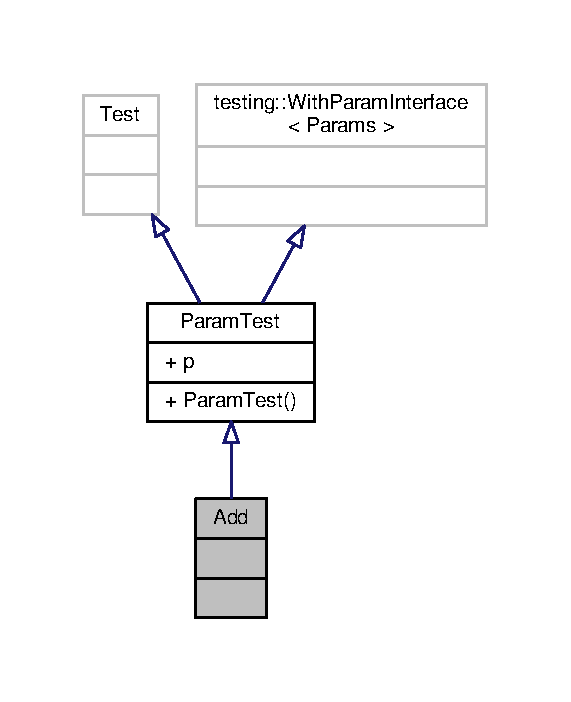
\includegraphics[width=274pt]{struct_add__inherit__graph}
\end{center}
\end{figure}


Collaboration diagram for Add\+:
\nopagebreak
\begin{figure}[H]
\begin{center}
\leavevmode
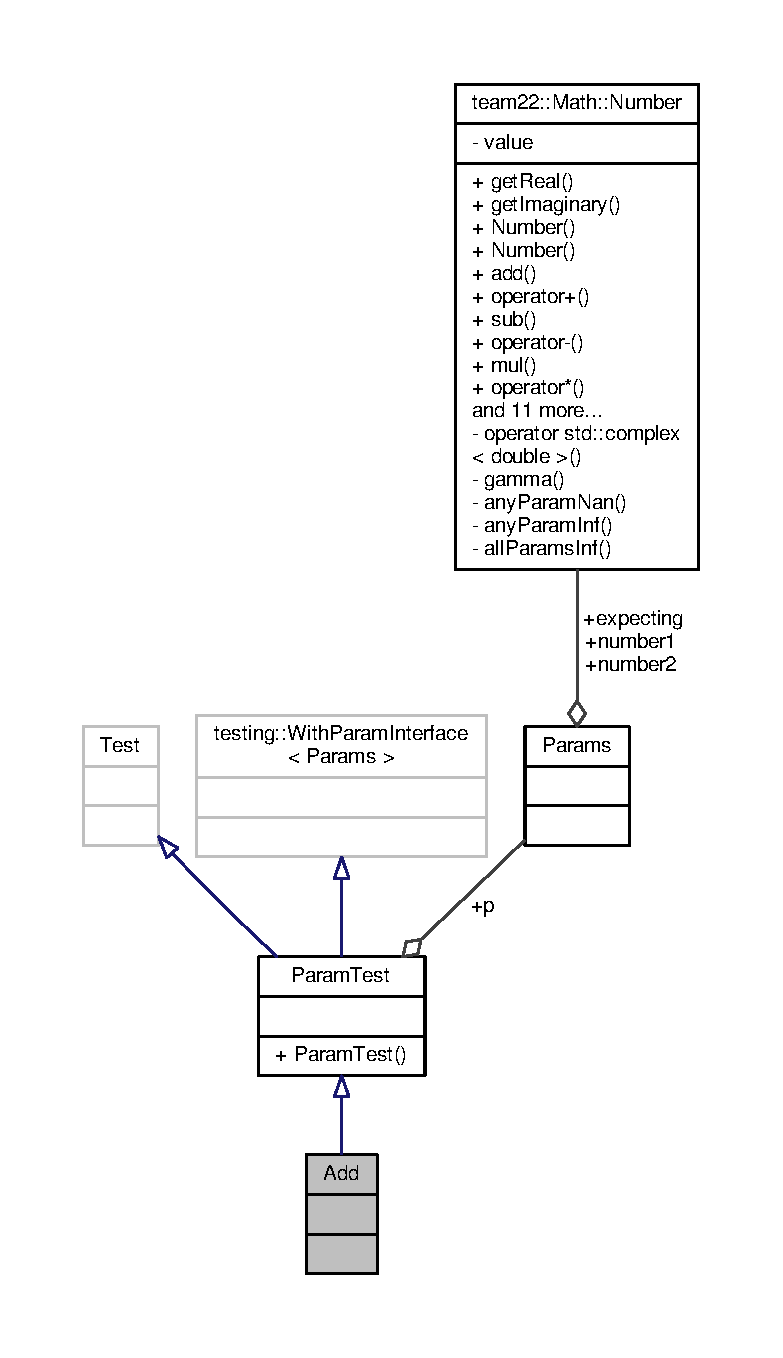
\includegraphics[height=550pt]{struct_add__coll__graph}
\end{center}
\end{figure}
\subsection*{Additional Inherited Members}


\subsection{Detailed Description}


Definition at line 74 of file Number\+Test.\+cpp.



The documentation for this struct was generated from the following file\+:\begin{DoxyCompactItemize}
\item 
src/tests/\hyperlink{_number_test_8cpp}{Number\+Test.\+cpp}\end{DoxyCompactItemize}

\hypertarget{class_backend_tester}{}\section{Backend\+Tester Class Reference}
\label{class_backend_tester}\index{Backend\+Tester@{Backend\+Tester}}


Inheritance diagram for Backend\+Tester\+:
\nopagebreak
\begin{figure}[H]
\begin{center}
\leavevmode
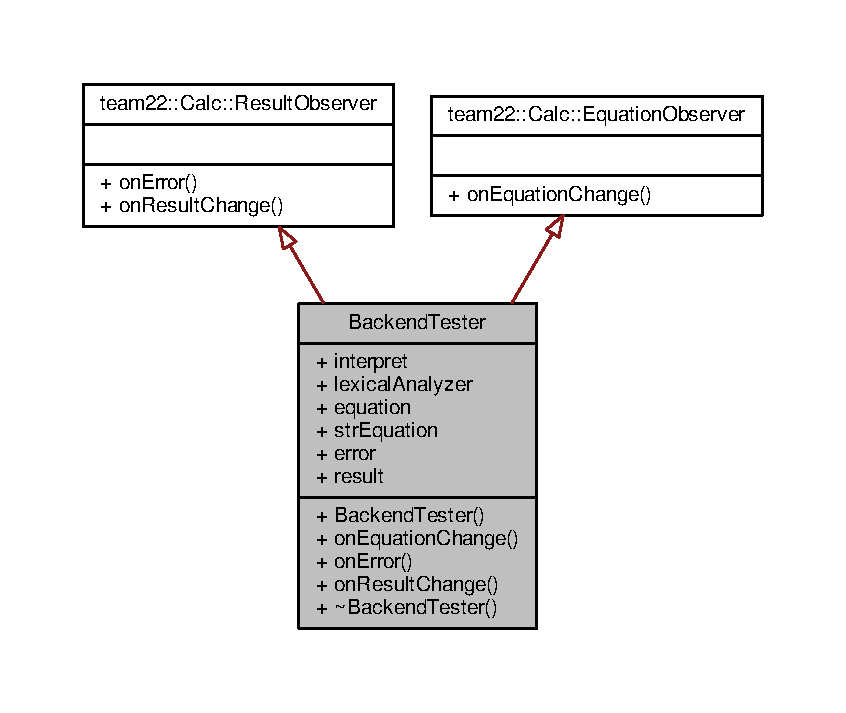
\includegraphics[width=350pt]{class_backend_tester__inherit__graph}
\end{center}
\end{figure}


Collaboration diagram for Backend\+Tester\+:
\nopagebreak
\begin{figure}[H]
\begin{center}
\leavevmode
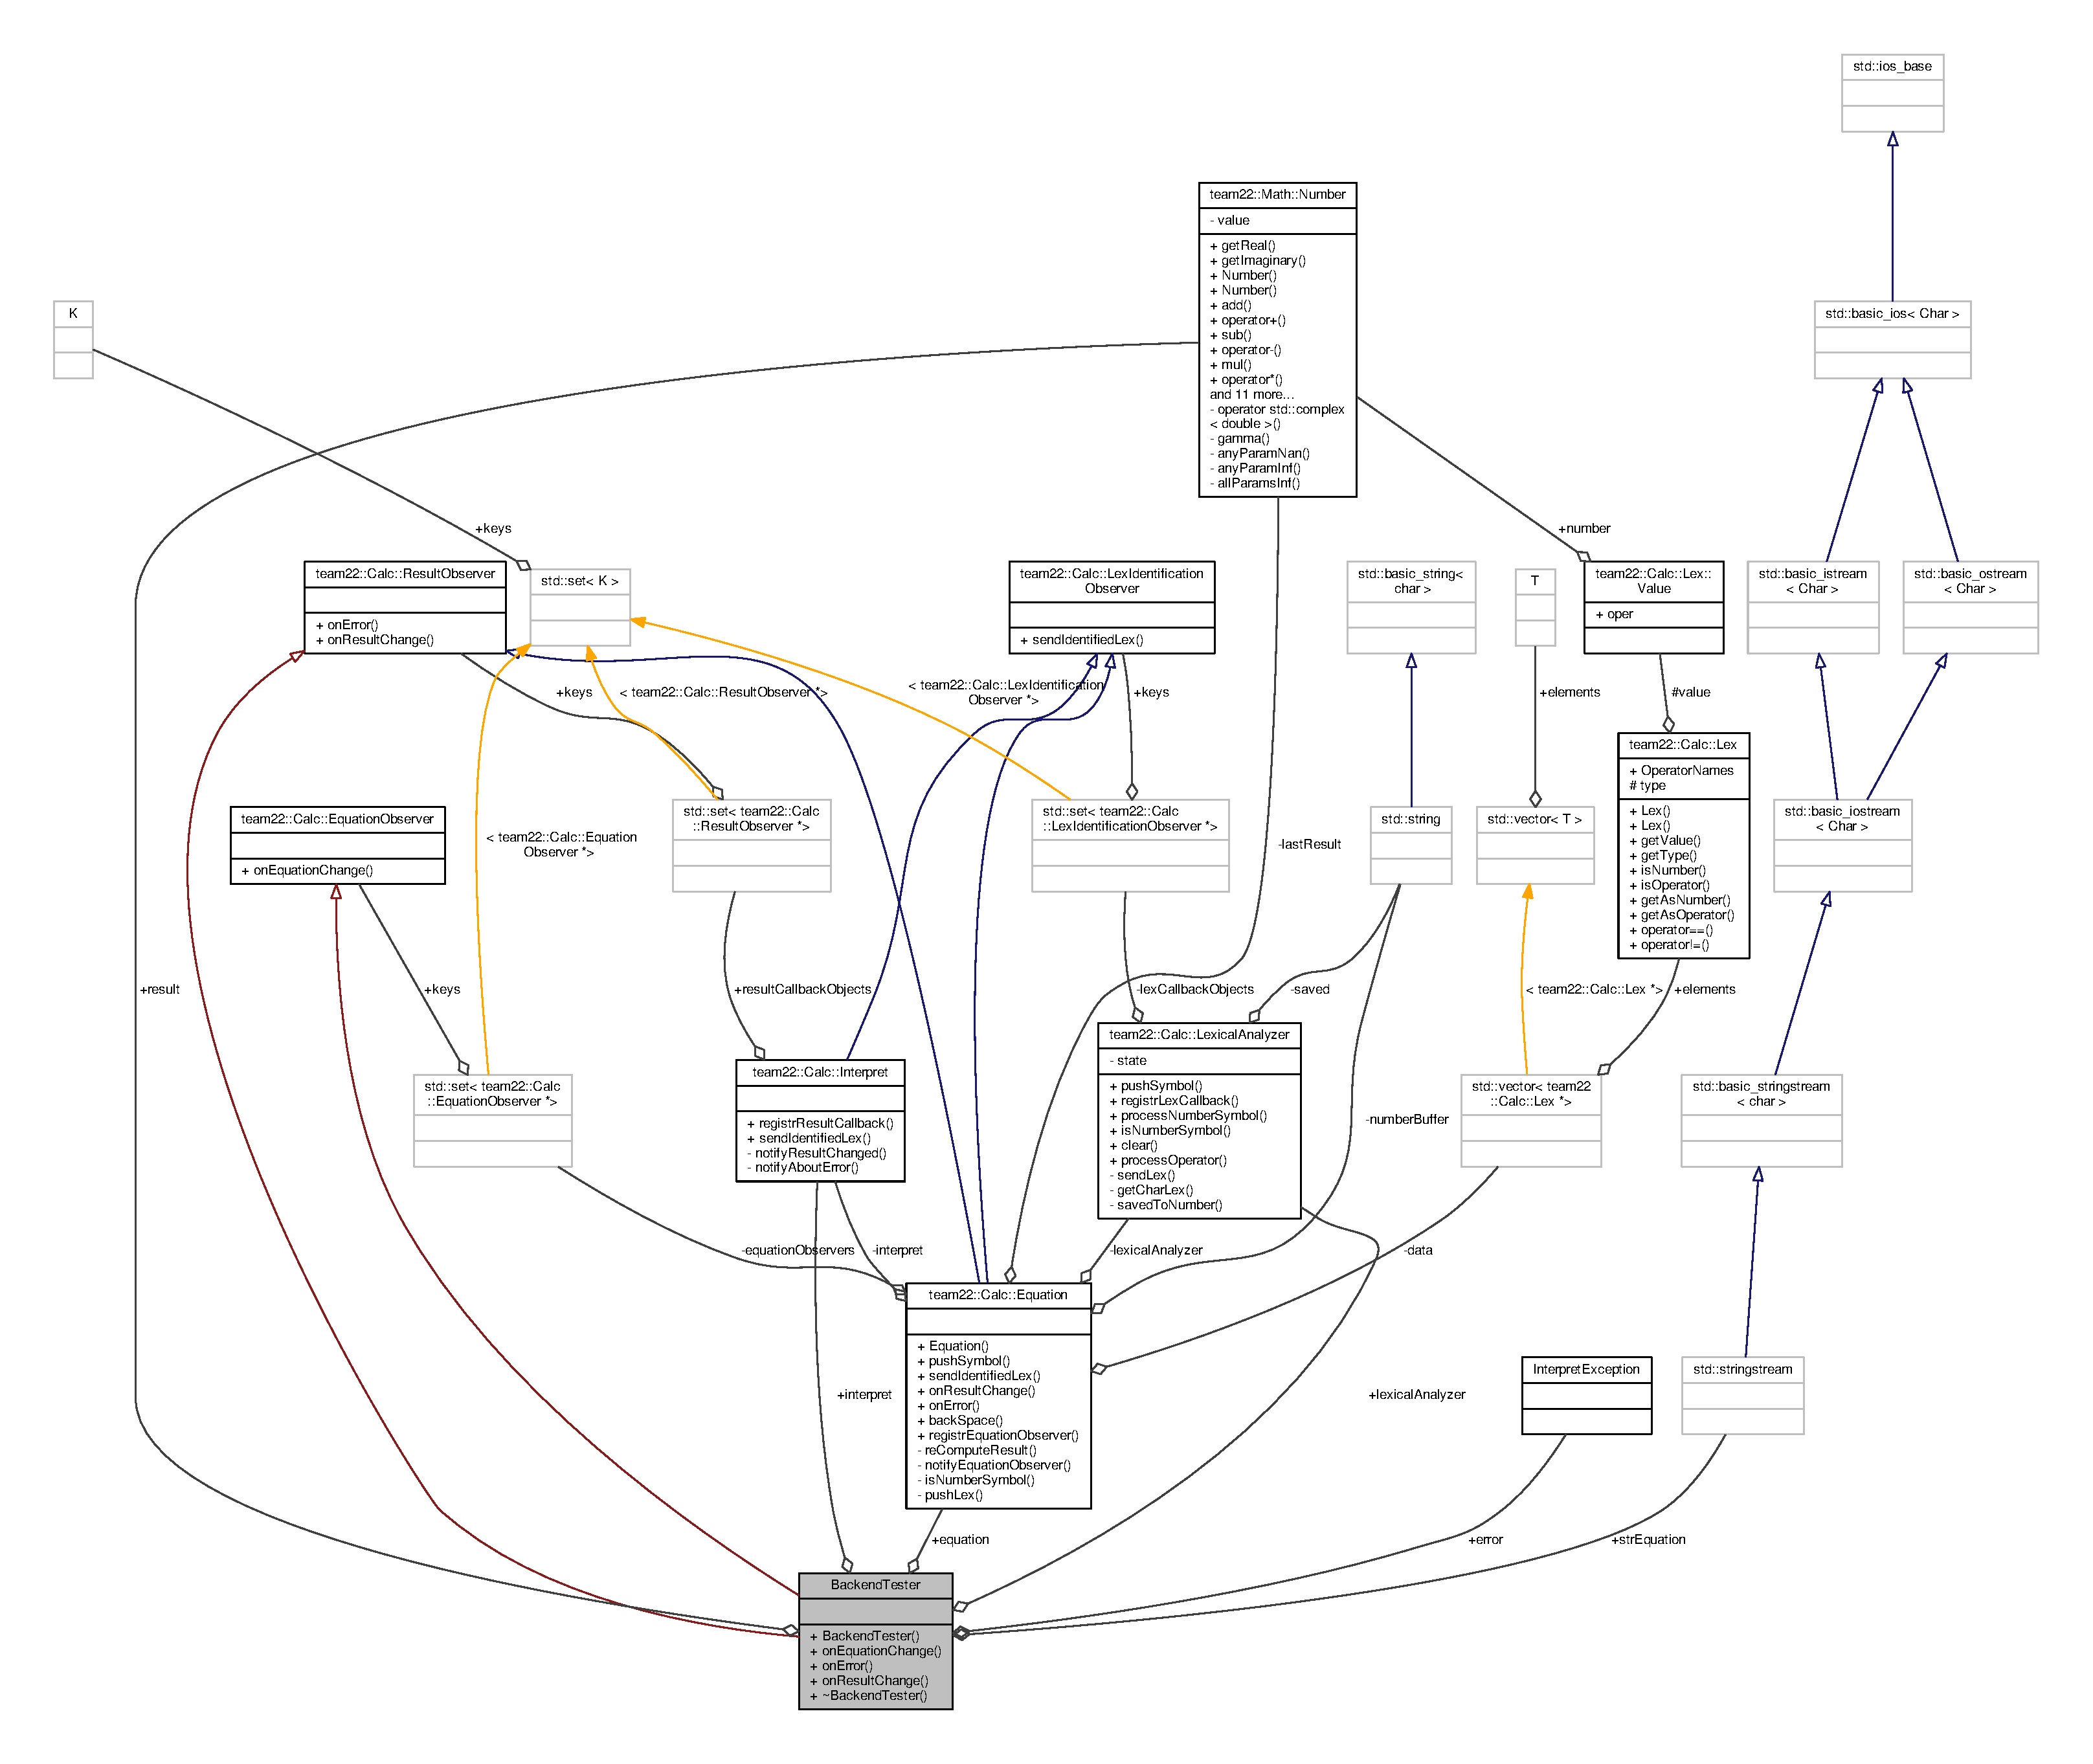
\includegraphics[width=350pt]{class_backend_tester__coll__graph}
\end{center}
\end{figure}
\subsection*{Public Member Functions}
\begin{DoxyCompactItemize}
\item 
\hyperlink{class_backend_tester_ad3927c00c9026acabc91277dce2b9980}{Backend\+Tester} ()
\item 
void \hyperlink{class_backend_tester_a9b7caf17f8ad274936fab5ca4bc669f8}{on\+Equation\+Change} () override
\item 
void \hyperlink{class_backend_tester_a9f83f432f7d71304026ff07caf20a65d}{on\+Error} (\hyperlink{class_interpret_exception}{Interpret\+Exception} exception) override
\item 
void \hyperlink{class_backend_tester_af84da1816cef621e57c65a01aa26d66e}{on\+Result\+Change} (\hyperlink{classteam22_1_1_math_1_1_number}{team22\+::\+Math\+::\+Number} \hyperlink{class_backend_tester_a4c0eeb2e7a5f1ef876b6e61fdb1701fc}{result}) override
\item 
virtual \hyperlink{class_backend_tester_a02c1da72606e5b3683b642564af9611d}{$\sim$\+Backend\+Tester} ()
\end{DoxyCompactItemize}
\subsection*{Public Attributes}
\begin{DoxyCompactItemize}
\item 
\hyperlink{classteam22_1_1_calc_1_1_interpret}{Interpret} \hyperlink{class_backend_tester_ae033438ca3f49eeb6f1f8932fd17b717}{interpret}
\item 
\hyperlink{classteam22_1_1_calc_1_1_lexical_analyzer}{Lexical\+Analyzer} \hyperlink{class_backend_tester_a7dd738e95d26936889aefa439540698d}{lexical\+Analyzer}
\item 
\hyperlink{classteam22_1_1_calc_1_1_equation}{Equation} \hyperlink{class_backend_tester_a72e182a9a678f3c9dc6daf2bb8afb711}{equation}
\item 
stringstream \hyperlink{class_backend_tester_ac42c696a31021852c1868c2e45f1d8b1}{str\+Equation}
\item 
\hyperlink{class_interpret_exception}{Interpret\+Exception} $\ast$ \hyperlink{class_backend_tester_a8b8308a2c21881f287a49951792b2e0d}{error} = nullptr
\item 
\hyperlink{classteam22_1_1_math_1_1_number}{Number} \hyperlink{class_backend_tester_a4c0eeb2e7a5f1ef876b6e61fdb1701fc}{result} = \{0\}
\end{DoxyCompactItemize}
\subsection*{Additional Inherited Members}


\subsection{Detailed Description}


Definition at line 21 of file backend\+Test.\+cpp.



\subsection{Constructor \& Destructor Documentation}
\mbox{\Hypertarget{class_backend_tester_ad3927c00c9026acabc91277dce2b9980}\label{class_backend_tester_ad3927c00c9026acabc91277dce2b9980}} 
\index{Backend\+Tester@{Backend\+Tester}!Backend\+Tester@{Backend\+Tester}}
\index{Backend\+Tester@{Backend\+Tester}!Backend\+Tester@{Backend\+Tester}}
\subsubsection{\texorpdfstring{Backend\+Tester()}{BackendTester()}}
{\footnotesize\ttfamily Backend\+Tester\+::\+Backend\+Tester (\begin{DoxyParamCaption}{ }\end{DoxyParamCaption})\hspace{0.3cm}{\ttfamily [inline]}}



Definition at line 31 of file backend\+Test.\+cpp.



References team22\+::\+Calc\+::\+Equation\+::registr\+Equation\+Observer(), team22\+::\+Calc\+::\+Lexical\+Analyzer\+::registr\+Lex\+Callback(), and team22\+::\+Calc\+::\+Interpret\+::registr\+Result\+Callback().

\mbox{\Hypertarget{class_backend_tester_a02c1da72606e5b3683b642564af9611d}\label{class_backend_tester_a02c1da72606e5b3683b642564af9611d}} 
\index{Backend\+Tester@{Backend\+Tester}!````~Backend\+Tester@{$\sim$\+Backend\+Tester}}
\index{````~Backend\+Tester@{$\sim$\+Backend\+Tester}!Backend\+Tester@{Backend\+Tester}}
\subsubsection{\texorpdfstring{$\sim$\+Backend\+Tester()}{~BackendTester()}}
{\footnotesize\ttfamily virtual Backend\+Tester\+::$\sim$\+Backend\+Tester (\begin{DoxyParamCaption}{ }\end{DoxyParamCaption})\hspace{0.3cm}{\ttfamily [inline]}, {\ttfamily [virtual]}}



Definition at line 55 of file backend\+Test.\+cpp.



\subsection{Member Function Documentation}
\mbox{\Hypertarget{class_backend_tester_a9b7caf17f8ad274936fab5ca4bc669f8}\label{class_backend_tester_a9b7caf17f8ad274936fab5ca4bc669f8}} 
\index{Backend\+Tester@{Backend\+Tester}!on\+Equation\+Change@{on\+Equation\+Change}}
\index{on\+Equation\+Change@{on\+Equation\+Change}!Backend\+Tester@{Backend\+Tester}}
\subsubsection{\texorpdfstring{on\+Equation\+Change()}{onEquationChange()}}
{\footnotesize\ttfamily void Backend\+Tester\+::on\+Equation\+Change (\begin{DoxyParamCaption}{ }\end{DoxyParamCaption})\hspace{0.3cm}{\ttfamily [inline]}, {\ttfamily [override]}, {\ttfamily [virtual]}}



Implements \hyperlink{classteam22_1_1_calc_1_1_equation_observer_a2fc2a1f8583f27b0087ff6053895ef25}{team22\+::\+Calc\+::\+Equation\+Observer}.



Definition at line 39 of file backend\+Test.\+cpp.

\mbox{\Hypertarget{class_backend_tester_a9f83f432f7d71304026ff07caf20a65d}\label{class_backend_tester_a9f83f432f7d71304026ff07caf20a65d}} 
\index{Backend\+Tester@{Backend\+Tester}!on\+Error@{on\+Error}}
\index{on\+Error@{on\+Error}!Backend\+Tester@{Backend\+Tester}}
\subsubsection{\texorpdfstring{on\+Error()}{onError()}}
{\footnotesize\ttfamily void Backend\+Tester\+::on\+Error (\begin{DoxyParamCaption}\item[{\hyperlink{class_interpret_exception}{Interpret\+Exception}}]{exception }\end{DoxyParamCaption})\hspace{0.3cm}{\ttfamily [inline]}, {\ttfamily [override]}, {\ttfamily [virtual]}}

Callback volaný pokud vznikla chyba při výpočtu 
\begin{DoxyParams}{Parameters}
{\em \hyperlink{class_interpret_exception}{Interpret\+Exception}} & \\
\hline
\end{DoxyParams}


Implements \hyperlink{classteam22_1_1_calc_1_1_result_observer_ad36cf8df89853d60f91094800c01d329}{team22\+::\+Calc\+::\+Result\+Observer}.



Definition at line 45 of file backend\+Test.\+cpp.

\mbox{\Hypertarget{class_backend_tester_af84da1816cef621e57c65a01aa26d66e}\label{class_backend_tester_af84da1816cef621e57c65a01aa26d66e}} 
\index{Backend\+Tester@{Backend\+Tester}!on\+Result\+Change@{on\+Result\+Change}}
\index{on\+Result\+Change@{on\+Result\+Change}!Backend\+Tester@{Backend\+Tester}}
\subsubsection{\texorpdfstring{on\+Result\+Change()}{onResultChange()}}
{\footnotesize\ttfamily void Backend\+Tester\+::on\+Result\+Change (\begin{DoxyParamCaption}\item[{\hyperlink{classteam22_1_1_math_1_1_number}{team22\+::\+Math\+::\+Number}}]{result }\end{DoxyParamCaption})\hspace{0.3cm}{\ttfamily [inline]}, {\ttfamily [override]}, {\ttfamily [virtual]}}

Callback volaný při změně výsledku 
\begin{DoxyParams}{Parameters}
{\em result} & \\
\hline
\end{DoxyParams}


Implements \hyperlink{classteam22_1_1_calc_1_1_result_observer_aa04007df3aa8a499c3a511f549238285}{team22\+::\+Calc\+::\+Result\+Observer}.



Definition at line 50 of file backend\+Test.\+cpp.



\subsection{Member Data Documentation}
\mbox{\Hypertarget{class_backend_tester_a72e182a9a678f3c9dc6daf2bb8afb711}\label{class_backend_tester_a72e182a9a678f3c9dc6daf2bb8afb711}} 
\index{Backend\+Tester@{Backend\+Tester}!equation@{equation}}
\index{equation@{equation}!Backend\+Tester@{Backend\+Tester}}
\subsubsection{\texorpdfstring{equation}{equation}}
{\footnotesize\ttfamily \hyperlink{classteam22_1_1_calc_1_1_equation}{Equation} Backend\+Tester\+::equation}



Definition at line 26 of file backend\+Test.\+cpp.



Referenced by T\+E\+S\+T().

\mbox{\Hypertarget{class_backend_tester_a8b8308a2c21881f287a49951792b2e0d}\label{class_backend_tester_a8b8308a2c21881f287a49951792b2e0d}} 
\index{Backend\+Tester@{Backend\+Tester}!error@{error}}
\index{error@{error}!Backend\+Tester@{Backend\+Tester}}
\subsubsection{\texorpdfstring{error}{error}}
{\footnotesize\ttfamily \hyperlink{class_interpret_exception}{Interpret\+Exception}$\ast$ Backend\+Tester\+::error = nullptr}



Definition at line 28 of file backend\+Test.\+cpp.



Referenced by T\+E\+S\+T().

\mbox{\Hypertarget{class_backend_tester_ae033438ca3f49eeb6f1f8932fd17b717}\label{class_backend_tester_ae033438ca3f49eeb6f1f8932fd17b717}} 
\index{Backend\+Tester@{Backend\+Tester}!interpret@{interpret}}
\index{interpret@{interpret}!Backend\+Tester@{Backend\+Tester}}
\subsubsection{\texorpdfstring{interpret}{interpret}}
{\footnotesize\ttfamily \hyperlink{classteam22_1_1_calc_1_1_interpret}{Interpret} Backend\+Tester\+::interpret}



Definition at line 24 of file backend\+Test.\+cpp.

\mbox{\Hypertarget{class_backend_tester_a7dd738e95d26936889aefa439540698d}\label{class_backend_tester_a7dd738e95d26936889aefa439540698d}} 
\index{Backend\+Tester@{Backend\+Tester}!lexical\+Analyzer@{lexical\+Analyzer}}
\index{lexical\+Analyzer@{lexical\+Analyzer}!Backend\+Tester@{Backend\+Tester}}
\subsubsection{\texorpdfstring{lexical\+Analyzer}{lexicalAnalyzer}}
{\footnotesize\ttfamily \hyperlink{classteam22_1_1_calc_1_1_lexical_analyzer}{Lexical\+Analyzer} Backend\+Tester\+::lexical\+Analyzer}



Definition at line 25 of file backend\+Test.\+cpp.

\mbox{\Hypertarget{class_backend_tester_a4c0eeb2e7a5f1ef876b6e61fdb1701fc}\label{class_backend_tester_a4c0eeb2e7a5f1ef876b6e61fdb1701fc}} 
\index{Backend\+Tester@{Backend\+Tester}!result@{result}}
\index{result@{result}!Backend\+Tester@{Backend\+Tester}}
\subsubsection{\texorpdfstring{result}{result}}
{\footnotesize\ttfamily \hyperlink{classteam22_1_1_math_1_1_number}{Number} Backend\+Tester\+::result = \{0\}}



Definition at line 29 of file backend\+Test.\+cpp.



Referenced by T\+E\+S\+T().

\mbox{\Hypertarget{class_backend_tester_ac42c696a31021852c1868c2e45f1d8b1}\label{class_backend_tester_ac42c696a31021852c1868c2e45f1d8b1}} 
\index{Backend\+Tester@{Backend\+Tester}!str\+Equation@{str\+Equation}}
\index{str\+Equation@{str\+Equation}!Backend\+Tester@{Backend\+Tester}}
\subsubsection{\texorpdfstring{str\+Equation}{strEquation}}
{\footnotesize\ttfamily stringstream Backend\+Tester\+::str\+Equation}



Definition at line 27 of file backend\+Test.\+cpp.



Referenced by T\+E\+S\+T().



The documentation for this class was generated from the following file\+:\begin{DoxyCompactItemize}
\item 
tests/\hyperlink{backend_test_8cpp}{backend\+Test.\+cpp}\end{DoxyCompactItemize}

\hypertarget{struct_div}{}\section{Div Struct Reference}
\label{struct_div}\index{Div@{Div}}


Inheritance diagram for Div\+:
\nopagebreak
\begin{figure}[H]
\begin{center}
\leavevmode
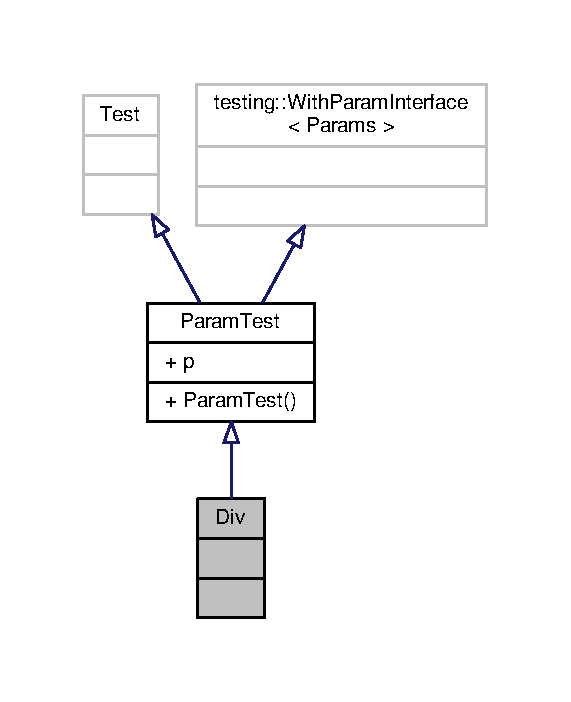
\includegraphics[width=274pt]{struct_div__inherit__graph}
\end{center}
\end{figure}


Collaboration diagram for Div\+:
\nopagebreak
\begin{figure}[H]
\begin{center}
\leavevmode
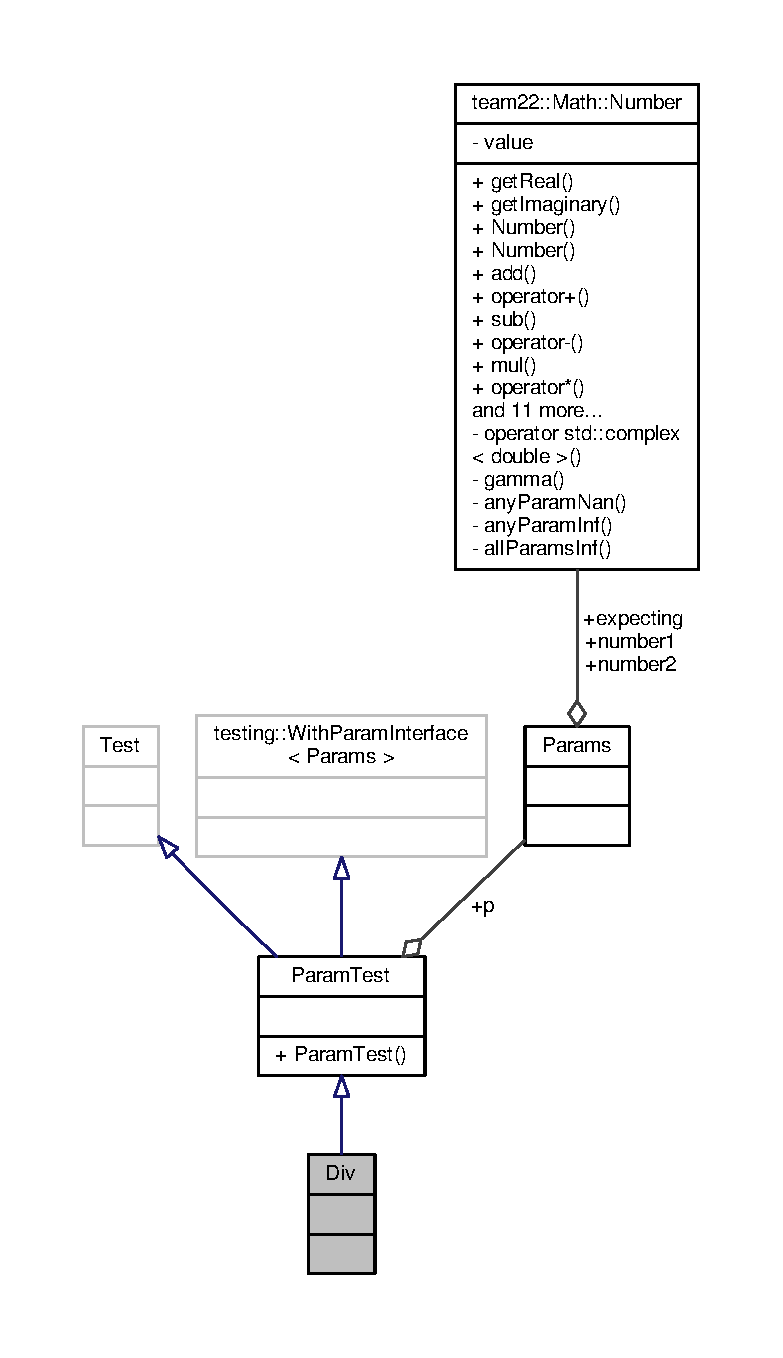
\includegraphics[height=550pt]{struct_div__coll__graph}
\end{center}
\end{figure}
\subsection*{Additional Inherited Members}


\subsection{Detailed Description}


Definition at line 76 of file Number\+Test.\+cpp.



The documentation for this struct was generated from the following file\+:\begin{DoxyCompactItemize}
\item 
tests/\hyperlink{_number_test_8cpp}{Number\+Test.\+cpp}\end{DoxyCompactItemize}

\hypertarget{classteam22_1_1_calc_1_1_equation}{}\section{team22\+:\+:Calc\+:\+:Equation Class Reference}
\label{classteam22_1_1_calc_1_1_equation}\index{team22\+::\+Calc\+::\+Equation@{team22\+::\+Calc\+::\+Equation}}


Třída reprezentující rovnici.  




{\ttfamily \#include $<$Equation.\+h$>$}



Inheritance diagram for team22\+:\+:Calc\+:\+:Equation\+:
\nopagebreak
\begin{figure}[H]
\begin{center}
\leavevmode
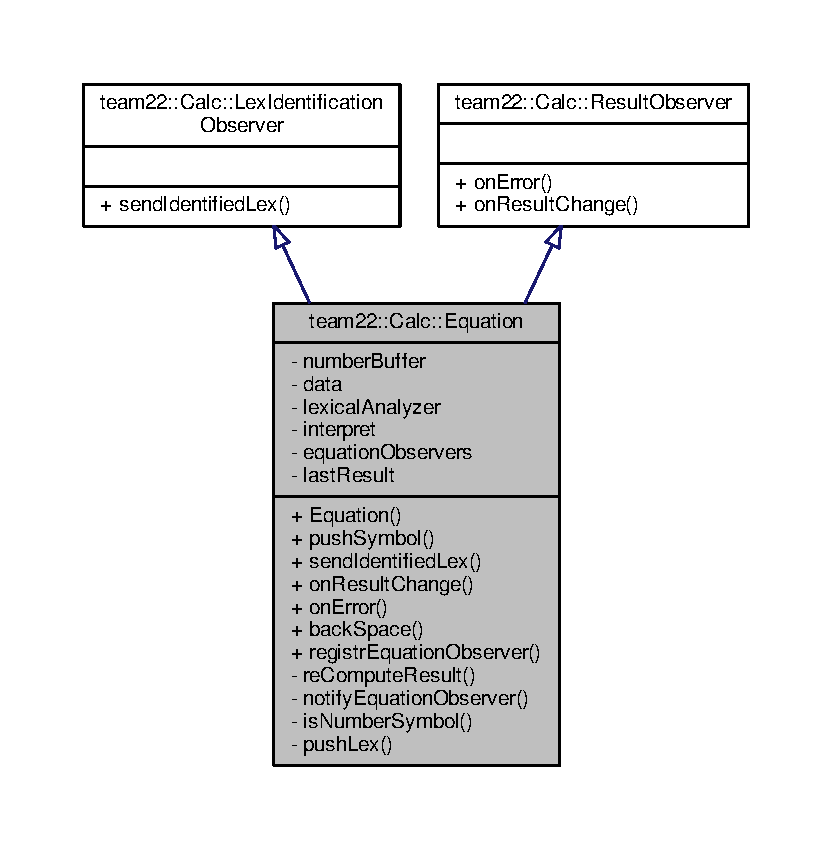
\includegraphics[width=350pt]{classteam22_1_1_calc_1_1_equation__inherit__graph}
\end{center}
\end{figure}


Collaboration diagram for team22\+:\+:Calc\+:\+:Equation\+:
\nopagebreak
\begin{figure}[H]
\begin{center}
\leavevmode
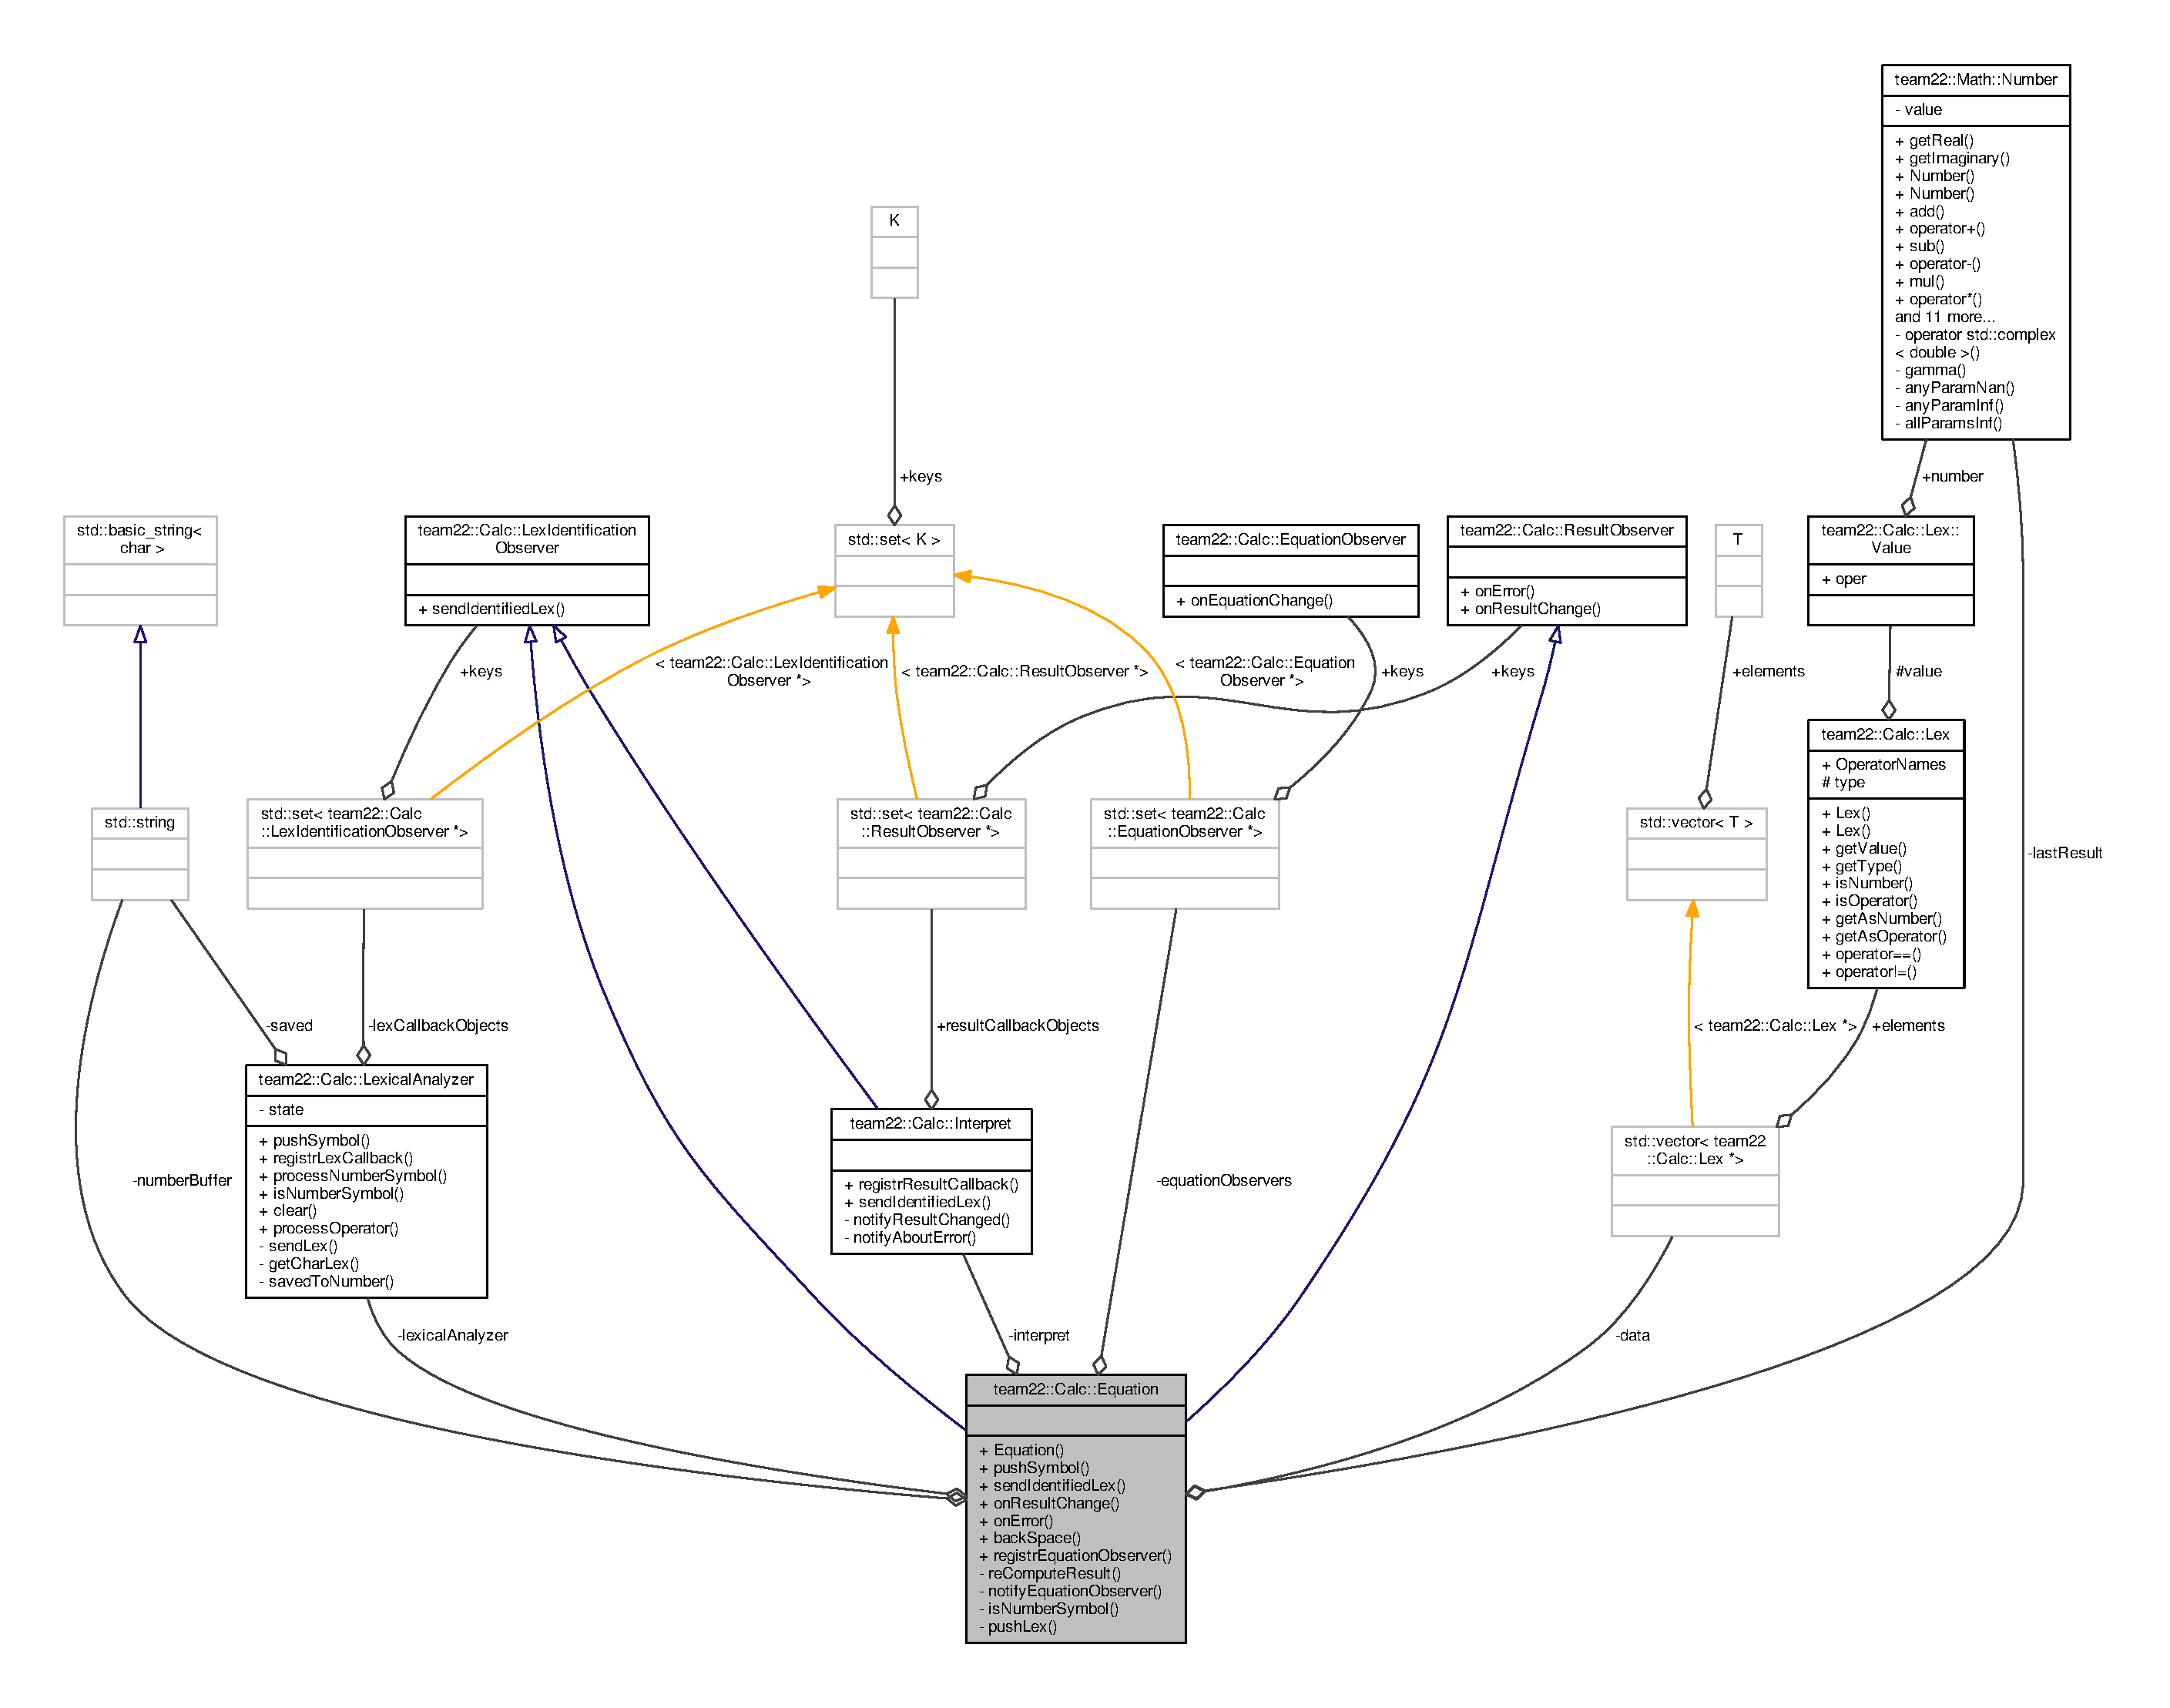
\includegraphics[width=350pt]{classteam22_1_1_calc_1_1_equation__coll__graph}
\end{center}
\end{figure}
\subsection*{Public Member Functions}
\begin{DoxyCompactItemize}
\item 
\hyperlink{classteam22_1_1_calc_1_1_equation_a085dc8be6e009511735b8c317d951610}{Equation} (\hyperlink{classteam22_1_1_calc_1_1_lexical_analyzer}{Lexical\+Analyzer} \&\hyperlink{classteam22_1_1_calc_1_1_equation_a65aeaa2a279994b03517a22addf31fc1}{lexical\+Analyzer}, \hyperlink{classteam22_1_1_calc_1_1_interpret}{Interpret} \&\hyperlink{classteam22_1_1_calc_1_1_equation_a8812a84e9c0f194eba491b0dba0cb015}{interpret})
\item 
void \hyperlink{classteam22_1_1_calc_1_1_equation_a324bf6372508c1b931c5ad8f39ccf8c4}{push\+Symbol} (char symbol)
\item 
void \hyperlink{classteam22_1_1_calc_1_1_equation_ad5768951865500ec7fc514f676de2851}{send\+Identified\+Lex} (\hyperlink{classteam22_1_1_calc_1_1_lex}{Lex} lex) override
\item 
void \hyperlink{classteam22_1_1_calc_1_1_equation_a302c295e099f589897a1bad4b02d3de8}{on\+Result\+Change} (\hyperlink{classteam22_1_1_math_1_1_number}{Math\+::\+Number} result) override
\item 
void \hyperlink{classteam22_1_1_calc_1_1_equation_a4e7a0614867931bcc714440441cdd894}{on\+Error} (\hyperlink{class_interpret_exception}{Interpret\+Exception} exception) override
\item 
void \hyperlink{classteam22_1_1_calc_1_1_equation_acccaaf8d823e6f1b7f6831fc0c8c4a62}{back\+Space} ()
\begin{DoxyCompactList}\small\item\em Provede operaci backspace Pokud je rovnice zakončena číslem odstraní poslední číslici jinak poslední lexem (operator) přepočítá rovnici. \end{DoxyCompactList}\item 
void \hyperlink{classteam22_1_1_calc_1_1_equation_a705c26d64f67f673e4919494d7e22d4a}{registr\+Equation\+Observer} (\hyperlink{classteam22_1_1_calc_1_1_equation_observer}{Equation\+Observer} $\ast$\hyperlink{classteam22_1_1_calc_1_1_equation_a76439666b11701dd1c42507397c5a316}{equation\+Observers})
\end{DoxyCompactItemize}
\subsection*{Private Member Functions}
\begin{DoxyCompactItemize}
\item 
void \hyperlink{classteam22_1_1_calc_1_1_equation_aba44b10dfb0ece96f3e0279d34cec868}{re\+Compute\+Result} ()
\item 
void \hyperlink{classteam22_1_1_calc_1_1_equation_acb90f7fefbd20c57864de0ed691bb65f}{notify\+Equation\+Observer} ()
\item 
bool \hyperlink{classteam22_1_1_calc_1_1_equation_afa4b44cfa408f74370851f7f64f55743}{is\+Number\+Symbol} (char \&symbol)
\item 
void \hyperlink{classteam22_1_1_calc_1_1_equation_af17ea6795813114d578e17109325d5e9}{push\+Lex} (\hyperlink{classteam22_1_1_calc_1_1_lex}{Lex} $\ast$lex)
\end{DoxyCompactItemize}
\subsection*{Private Attributes}
\begin{DoxyCompactItemize}
\item 
std\+::string \hyperlink{classteam22_1_1_calc_1_1_equation_a816d00b732bc472768b41da216a4335c}{number\+Buffer}
\item 
std\+::vector$<$ \hyperlink{classteam22_1_1_calc_1_1_lex}{Lex} $\ast$ $>$ \hyperlink{classteam22_1_1_calc_1_1_equation_ab02c12c6e452d5271f26bbae073ed4dc}{data}
\item 
\hyperlink{classteam22_1_1_calc_1_1_lexical_analyzer}{Lexical\+Analyzer} \hyperlink{classteam22_1_1_calc_1_1_equation_a65aeaa2a279994b03517a22addf31fc1}{lexical\+Analyzer}
\item 
\hyperlink{classteam22_1_1_calc_1_1_interpret}{Interpret} \hyperlink{classteam22_1_1_calc_1_1_equation_a8812a84e9c0f194eba491b0dba0cb015}{interpret}
\item 
std\+::set$<$ \hyperlink{classteam22_1_1_calc_1_1_equation_observer}{Equation\+Observer} $\ast$ $>$ \hyperlink{classteam22_1_1_calc_1_1_equation_a76439666b11701dd1c42507397c5a316}{equation\+Observers}
\item 
\hyperlink{classteam22_1_1_math_1_1_number}{Math\+::\+Number} \hyperlink{classteam22_1_1_calc_1_1_equation_a7c62440412a33b3b3300e63ff65ffafb}{last\+Result} = \{0\}
\end{DoxyCompactItemize}
\subsection*{Friends}
\begin{DoxyCompactItemize}
\item 
std\+::stringstream \& \hyperlink{classteam22_1_1_calc_1_1_equation_a8ee0e20eaa10e114d79e0b16cb11ddcf}{operator$<$$<$} (std\+::stringstream \&os, const \hyperlink{classteam22_1_1_calc_1_1_equation}{Equation} \&equation)
\item 
std\+::ostream \& \hyperlink{classteam22_1_1_calc_1_1_equation_aea7df9bdea5430cc309e17f1f2fbe78f}{operator$<$$<$} (std\+::ostream \&os, const \hyperlink{classteam22_1_1_calc_1_1_equation}{Equation} \&equation)
\end{DoxyCompactItemize}


\subsection{Detailed Description}
Třída reprezentující rovnici. 

Třída přebírá znaky a předává je Lexikálnímu analyzátoru, dále pozoruje Identifikaci Lexému. Při každé změně rovnice třída upozorní své pozorovatele o této změně. Pokud příjme lexem \hyperlink{classteam22_1_1_calc_1_1_lex_a61d29fc4878a3b36d2de2f13c56ed932ac62fe9cff8a15f20fb1416612309ae80}{Lex\+::\+BS} odebere číslici(i beru jako číslici) či operátor z konce rovnice a rovnici přepočítá Pokud příjme lexem \hyperlink{classteam22_1_1_calc_1_1_lex_a61d29fc4878a3b36d2de2f13c56ed932a4281d7ef6ac8dbf79c87603ca20c351c}{Lex\+::\+C\+L\+E\+AR} rovnice se smaže, Operátory \hyperlink{classteam22_1_1_calc_1_1_lex_a61d29fc4878a3b36d2de2f13c56ed932ac62fe9cff8a15f20fb1416612309ae80}{Lex\+::\+BS} \hyperlink{classteam22_1_1_calc_1_1_lex_a61d29fc4878a3b36d2de2f13c56ed932a4281d7ef6ac8dbf79c87603ca20c351c}{Lex\+::\+C\+L\+E\+AR} a \hyperlink{classteam22_1_1_calc_1_1_lex_a61d29fc4878a3b36d2de2f13c56ed932a3c1443c79523cadf6582f238c04a015f}{Lex\+::\+E\+V\+AL} se do rovnice nezapisují. Po \hyperlink{classteam22_1_1_calc_1_1_lex_a61d29fc4878a3b36d2de2f13c56ed932a3c1443c79523cadf6582f238c04a015f}{Lex\+::\+E\+V\+AL} pokud následuje číslo rovnice začíná tímto číslem a jinak začíná výsledkem předchozí rovnice pokud taková není 0. 

Definition at line 30 of file Equation.\+h.



\subsection{Constructor \& Destructor Documentation}
\mbox{\Hypertarget{classteam22_1_1_calc_1_1_equation_a085dc8be6e009511735b8c317d951610}\label{classteam22_1_1_calc_1_1_equation_a085dc8be6e009511735b8c317d951610}} 
\index{team22\+::\+Calc\+::\+Equation@{team22\+::\+Calc\+::\+Equation}!Equation@{Equation}}
\index{Equation@{Equation}!team22\+::\+Calc\+::\+Equation@{team22\+::\+Calc\+::\+Equation}}
\subsubsection{\texorpdfstring{Equation()}{Equation()}}
{\footnotesize\ttfamily Equation\+::\+Equation (\begin{DoxyParamCaption}\item[{\hyperlink{classteam22_1_1_calc_1_1_lexical_analyzer}{Lexical\+Analyzer} \&}]{lexical\+Analyzer,  }\item[{\hyperlink{classteam22_1_1_calc_1_1_interpret}{Interpret} \&}]{interpret }\end{DoxyParamCaption})}


\begin{DoxyParams}{Parameters}
{\em lexical\+Analyzer} & \\
\hline
{\em interpret} & \\
\hline
\end{DoxyParams}


Definition at line 106 of file Equation.\+cpp.



References team22\+::\+Calc\+::\+Lexical\+Analyzer\+::registr\+Lex\+Callback().



\subsection{Member Function Documentation}
\mbox{\Hypertarget{classteam22_1_1_calc_1_1_equation_acccaaf8d823e6f1b7f6831fc0c8c4a62}\label{classteam22_1_1_calc_1_1_equation_acccaaf8d823e6f1b7f6831fc0c8c4a62}} 
\index{team22\+::\+Calc\+::\+Equation@{team22\+::\+Calc\+::\+Equation}!back\+Space@{back\+Space}}
\index{back\+Space@{back\+Space}!team22\+::\+Calc\+::\+Equation@{team22\+::\+Calc\+::\+Equation}}
\subsubsection{\texorpdfstring{back\+Space()}{backSpace()}}
{\footnotesize\ttfamily void Equation\+::back\+Space (\begin{DoxyParamCaption}{ }\end{DoxyParamCaption})}



Provede operaci backspace Pokud je rovnice zakončena číslem odstraní poslední číslici jinak poslední lexem (operator) přepočítá rovnici. 



Definition at line 56 of file Equation.\+cpp.



References data, lexical\+Analyzer, number\+Buffer, team22\+::\+Calc\+::\+Lexical\+Analyzer\+::push\+Symbol(), and re\+Compute\+Result().



Referenced by send\+Identified\+Lex().

\mbox{\Hypertarget{classteam22_1_1_calc_1_1_equation_afa4b44cfa408f74370851f7f64f55743}\label{classteam22_1_1_calc_1_1_equation_afa4b44cfa408f74370851f7f64f55743}} 
\index{team22\+::\+Calc\+::\+Equation@{team22\+::\+Calc\+::\+Equation}!is\+Number\+Symbol@{is\+Number\+Symbol}}
\index{is\+Number\+Symbol@{is\+Number\+Symbol}!team22\+::\+Calc\+::\+Equation@{team22\+::\+Calc\+::\+Equation}}
\subsubsection{\texorpdfstring{is\+Number\+Symbol()}{isNumberSymbol()}}
{\footnotesize\ttfamily bool Equation\+::is\+Number\+Symbol (\begin{DoxyParamCaption}\item[{char \&}]{symbol }\end{DoxyParamCaption})\hspace{0.3cm}{\ttfamily [private]}}

Jedná se o znak čísla tedy číslici nebo i 

Definition at line 95 of file Equation.\+cpp.



Referenced by push\+Symbol().

\mbox{\Hypertarget{classteam22_1_1_calc_1_1_equation_acb90f7fefbd20c57864de0ed691bb65f}\label{classteam22_1_1_calc_1_1_equation_acb90f7fefbd20c57864de0ed691bb65f}} 
\index{team22\+::\+Calc\+::\+Equation@{team22\+::\+Calc\+::\+Equation}!notify\+Equation\+Observer@{notify\+Equation\+Observer}}
\index{notify\+Equation\+Observer@{notify\+Equation\+Observer}!team22\+::\+Calc\+::\+Equation@{team22\+::\+Calc\+::\+Equation}}
\subsubsection{\texorpdfstring{notify\+Equation\+Observer()}{notifyEquationObserver()}}
{\footnotesize\ttfamily void Equation\+::notify\+Equation\+Observer (\begin{DoxyParamCaption}{ }\end{DoxyParamCaption})\hspace{0.3cm}{\ttfamily [private]}}

upozorní odebíratele na změnu rovnice 

Definition at line 89 of file Equation.\+cpp.



References equation\+Observers.



Referenced by push\+Symbol(), and send\+Identified\+Lex().

\mbox{\Hypertarget{classteam22_1_1_calc_1_1_equation_a4e7a0614867931bcc714440441cdd894}\label{classteam22_1_1_calc_1_1_equation_a4e7a0614867931bcc714440441cdd894}} 
\index{team22\+::\+Calc\+::\+Equation@{team22\+::\+Calc\+::\+Equation}!on\+Error@{on\+Error}}
\index{on\+Error@{on\+Error}!team22\+::\+Calc\+::\+Equation@{team22\+::\+Calc\+::\+Equation}}
\subsubsection{\texorpdfstring{on\+Error()}{onError()}}
{\footnotesize\ttfamily void Equation\+::on\+Error (\begin{DoxyParamCaption}\item[{\hyperlink{class_interpret_exception}{Interpret\+Exception}}]{exception }\end{DoxyParamCaption})\hspace{0.3cm}{\ttfamily [override]}, {\ttfamily [virtual]}}


\begin{DoxyParams}{Parameters}
{\em exception} & \\
\hline
\end{DoxyParams}


Implements \hyperlink{classteam22_1_1_calc_1_1_result_observer_ad36cf8df89853d60f91094800c01d329}{team22\+::\+Calc\+::\+Result\+Observer}.



Definition at line 122 of file Equation.\+cpp.



References data, and number\+Buffer.

\mbox{\Hypertarget{classteam22_1_1_calc_1_1_equation_a302c295e099f589897a1bad4b02d3de8}\label{classteam22_1_1_calc_1_1_equation_a302c295e099f589897a1bad4b02d3de8}} 
\index{team22\+::\+Calc\+::\+Equation@{team22\+::\+Calc\+::\+Equation}!on\+Result\+Change@{on\+Result\+Change}}
\index{on\+Result\+Change@{on\+Result\+Change}!team22\+::\+Calc\+::\+Equation@{team22\+::\+Calc\+::\+Equation}}
\subsubsection{\texorpdfstring{on\+Result\+Change()}{onResultChange()}}
{\footnotesize\ttfamily void Equation\+::on\+Result\+Change (\begin{DoxyParamCaption}\item[{\hyperlink{classteam22_1_1_math_1_1_number}{Math\+::\+Number}}]{result }\end{DoxyParamCaption})\hspace{0.3cm}{\ttfamily [override]}, {\ttfamily [virtual]}}


\begin{DoxyParams}{Parameters}
{\em result} & \\
\hline
\end{DoxyParams}


Implements \hyperlink{classteam22_1_1_calc_1_1_result_observer_aa04007df3aa8a499c3a511f549238285}{team22\+::\+Calc\+::\+Result\+Observer}.



Definition at line 117 of file Equation.\+cpp.



References last\+Result.

\mbox{\Hypertarget{classteam22_1_1_calc_1_1_equation_af17ea6795813114d578e17109325d5e9}\label{classteam22_1_1_calc_1_1_equation_af17ea6795813114d578e17109325d5e9}} 
\index{team22\+::\+Calc\+::\+Equation@{team22\+::\+Calc\+::\+Equation}!push\+Lex@{push\+Lex}}
\index{push\+Lex@{push\+Lex}!team22\+::\+Calc\+::\+Equation@{team22\+::\+Calc\+::\+Equation}}
\subsubsection{\texorpdfstring{push\+Lex()}{pushLex()}}
{\footnotesize\ttfamily void Equation\+::push\+Lex (\begin{DoxyParamCaption}\item[{\hyperlink{classteam22_1_1_calc_1_1_lex}{Lex} $\ast$}]{lex }\end{DoxyParamCaption})\hspace{0.3cm}{\ttfamily [private]}}

zpracuje příchozí Lexém 
\begin{DoxyParams}{Parameters}
{\em lex} & \\
\hline
\end{DoxyParams}


Definition at line 112 of file Equation.\+cpp.



References data.



Referenced by send\+Identified\+Lex().

\mbox{\Hypertarget{classteam22_1_1_calc_1_1_equation_a324bf6372508c1b931c5ad8f39ccf8c4}\label{classteam22_1_1_calc_1_1_equation_a324bf6372508c1b931c5ad8f39ccf8c4}} 
\index{team22\+::\+Calc\+::\+Equation@{team22\+::\+Calc\+::\+Equation}!push\+Symbol@{push\+Symbol}}
\index{push\+Symbol@{push\+Symbol}!team22\+::\+Calc\+::\+Equation@{team22\+::\+Calc\+::\+Equation}}
\subsubsection{\texorpdfstring{push\+Symbol()}{pushSymbol()}}
{\footnotesize\ttfamily void Equation\+::push\+Symbol (\begin{DoxyParamCaption}\item[{char}]{symbol }\end{DoxyParamCaption})}

Předání symbolu rovnici 
\begin{DoxyExceptions}{Exceptions}
{\em \hyperlink{classteam22_1_1_calc_1_1_lexical_analyzer_exception}{Lexical\+Analyzer\+Exception}} & \\
\hline
\end{DoxyExceptions}


Definition at line 45 of file Equation.\+cpp.



References is\+Number\+Symbol(), lexical\+Analyzer, notify\+Equation\+Observer(), number\+Buffer, and team22\+::\+Calc\+::\+Lexical\+Analyzer\+::push\+Symbol().



Referenced by T\+E\+S\+T().

\mbox{\Hypertarget{classteam22_1_1_calc_1_1_equation_aba44b10dfb0ece96f3e0279d34cec868}\label{classteam22_1_1_calc_1_1_equation_aba44b10dfb0ece96f3e0279d34cec868}} 
\index{team22\+::\+Calc\+::\+Equation@{team22\+::\+Calc\+::\+Equation}!re\+Compute\+Result@{re\+Compute\+Result}}
\index{re\+Compute\+Result@{re\+Compute\+Result}!team22\+::\+Calc\+::\+Equation@{team22\+::\+Calc\+::\+Equation}}
\subsubsection{\texorpdfstring{re\+Compute\+Result()}{reComputeResult()}}
{\footnotesize\ttfamily void Equation\+::re\+Compute\+Result (\begin{DoxyParamCaption}{ }\end{DoxyParamCaption})\hspace{0.3cm}{\ttfamily [private]}}

přepočítá výsledek 

Definition at line 100 of file Equation.\+cpp.



References data, interpret, and team22\+::\+Calc\+::\+Interpret\+::send\+Identified\+Lex().



Referenced by back\+Space().

\mbox{\Hypertarget{classteam22_1_1_calc_1_1_equation_a705c26d64f67f673e4919494d7e22d4a}\label{classteam22_1_1_calc_1_1_equation_a705c26d64f67f673e4919494d7e22d4a}} 
\index{team22\+::\+Calc\+::\+Equation@{team22\+::\+Calc\+::\+Equation}!registr\+Equation\+Observer@{registr\+Equation\+Observer}}
\index{registr\+Equation\+Observer@{registr\+Equation\+Observer}!team22\+::\+Calc\+::\+Equation@{team22\+::\+Calc\+::\+Equation}}
\subsubsection{\texorpdfstring{registr\+Equation\+Observer()}{registrEquationObserver()}}
{\footnotesize\ttfamily void Equation\+::registr\+Equation\+Observer (\begin{DoxyParamCaption}\item[{\hyperlink{classteam22_1_1_calc_1_1_equation_observer}{Equation\+Observer} $\ast$}]{equation\+Observers }\end{DoxyParamCaption})}

Zaregistruje pozorovatele změny rovnice 
\begin{DoxyParams}{Parameters}
{\em equation\+Observers} & \\
\hline
\end{DoxyParams}


Definition at line 84 of file Equation.\+cpp.



References equation\+Observers.



Referenced by Backend\+Tester\+::\+Backend\+Tester().

\mbox{\Hypertarget{classteam22_1_1_calc_1_1_equation_ad5768951865500ec7fc514f676de2851}\label{classteam22_1_1_calc_1_1_equation_ad5768951865500ec7fc514f676de2851}} 
\index{team22\+::\+Calc\+::\+Equation@{team22\+::\+Calc\+::\+Equation}!send\+Identified\+Lex@{send\+Identified\+Lex}}
\index{send\+Identified\+Lex@{send\+Identified\+Lex}!team22\+::\+Calc\+::\+Equation@{team22\+::\+Calc\+::\+Equation}}
\subsubsection{\texorpdfstring{send\+Identified\+Lex()}{sendIdentifiedLex()}}
{\footnotesize\ttfamily void Equation\+::send\+Identified\+Lex (\begin{DoxyParamCaption}\item[{\hyperlink{classteam22_1_1_calc_1_1_lex}{Lex}}]{lex }\end{DoxyParamCaption})\hspace{0.3cm}{\ttfamily [override]}, {\ttfamily [virtual]}}


\begin{DoxyParams}{Parameters}
{\em lex} & \\
\hline
\end{DoxyParams}


Implements \hyperlink{classteam22_1_1_calc_1_1_lex_identification_observer_ac139f75c560625ec6fdb2e34cf0d4884}{team22\+::\+Calc\+::\+Lex\+Identification\+Observer}.



Definition at line 15 of file Equation.\+cpp.



References back\+Space(), team22\+::\+Calc\+::\+Lex\+::\+BS, team22\+::\+Calc\+::\+Lex\+::\+C\+L\+E\+AR, data, team22\+::\+Calc\+::\+Lex\+::\+E\+V\+AL, team22\+::\+Calc\+::\+Lex\+::get\+As\+Operator(), interpret, team22\+::\+Calc\+::\+Lex\+::is\+Operator(), last\+Result, notify\+Equation\+Observer(), number\+Buffer, push\+Lex(), and team22\+::\+Calc\+::\+Interpret\+::send\+Identified\+Lex().



\subsection{Friends And Related Function Documentation}
\mbox{\Hypertarget{classteam22_1_1_calc_1_1_equation_a8ee0e20eaa10e114d79e0b16cb11ddcf}\label{classteam22_1_1_calc_1_1_equation_a8ee0e20eaa10e114d79e0b16cb11ddcf}} 
\index{team22\+::\+Calc\+::\+Equation@{team22\+::\+Calc\+::\+Equation}!operator$<$$<$@{operator$<$$<$}}
\index{operator$<$$<$@{operator$<$$<$}!team22\+::\+Calc\+::\+Equation@{team22\+::\+Calc\+::\+Equation}}
\subsubsection{\texorpdfstring{operator$<$$<$}{operator<<}\hspace{0.1cm}{\footnotesize\ttfamily [1/2]}}
{\footnotesize\ttfamily std\+::stringstream\& operator$<$$<$ (\begin{DoxyParamCaption}\item[{std\+::stringstream \&}]{os,  }\item[{const \hyperlink{classteam22_1_1_calc_1_1_equation}{Equation} \&}]{equation }\end{DoxyParamCaption})\hspace{0.3cm}{\ttfamily [friend]}}

\mbox{\Hypertarget{classteam22_1_1_calc_1_1_equation_aea7df9bdea5430cc309e17f1f2fbe78f}\label{classteam22_1_1_calc_1_1_equation_aea7df9bdea5430cc309e17f1f2fbe78f}} 
\index{team22\+::\+Calc\+::\+Equation@{team22\+::\+Calc\+::\+Equation}!operator$<$$<$@{operator$<$$<$}}
\index{operator$<$$<$@{operator$<$$<$}!team22\+::\+Calc\+::\+Equation@{team22\+::\+Calc\+::\+Equation}}
\subsubsection{\texorpdfstring{operator$<$$<$}{operator<<}\hspace{0.1cm}{\footnotesize\ttfamily [2/2]}}
{\footnotesize\ttfamily std\+::ostream\& operator$<$$<$ (\begin{DoxyParamCaption}\item[{std\+::ostream \&}]{os,  }\item[{const \hyperlink{classteam22_1_1_calc_1_1_equation}{Equation} \&}]{equation }\end{DoxyParamCaption})\hspace{0.3cm}{\ttfamily [friend]}}



\subsection{Member Data Documentation}
\mbox{\Hypertarget{classteam22_1_1_calc_1_1_equation_ab02c12c6e452d5271f26bbae073ed4dc}\label{classteam22_1_1_calc_1_1_equation_ab02c12c6e452d5271f26bbae073ed4dc}} 
\index{team22\+::\+Calc\+::\+Equation@{team22\+::\+Calc\+::\+Equation}!data@{data}}
\index{data@{data}!team22\+::\+Calc\+::\+Equation@{team22\+::\+Calc\+::\+Equation}}
\subsubsection{\texorpdfstring{data}{data}}
{\footnotesize\ttfamily std\+::vector$<$\hyperlink{classteam22_1_1_calc_1_1_lex}{Lex} $\ast$$>$ team22\+::\+Calc\+::\+Equation\+::data\hspace{0.3cm}{\ttfamily [private]}}

Lexémy tvořící rovnici 

Definition at line 42 of file Equation.\+h.



Referenced by back\+Space(), on\+Error(), push\+Lex(), re\+Compute\+Result(), and send\+Identified\+Lex().

\mbox{\Hypertarget{classteam22_1_1_calc_1_1_equation_a76439666b11701dd1c42507397c5a316}\label{classteam22_1_1_calc_1_1_equation_a76439666b11701dd1c42507397c5a316}} 
\index{team22\+::\+Calc\+::\+Equation@{team22\+::\+Calc\+::\+Equation}!equation\+Observers@{equation\+Observers}}
\index{equation\+Observers@{equation\+Observers}!team22\+::\+Calc\+::\+Equation@{team22\+::\+Calc\+::\+Equation}}
\subsubsection{\texorpdfstring{equation\+Observers}{equationObservers}}
{\footnotesize\ttfamily std\+::set$<$\hyperlink{classteam22_1_1_calc_1_1_equation_observer}{Equation\+Observer} $\ast$$>$ team22\+::\+Calc\+::\+Equation\+::equation\+Observers\hspace{0.3cm}{\ttfamily [private]}}

Pozorovatele 

Definition at line 59 of file Equation.\+h.



Referenced by notify\+Equation\+Observer(), and registr\+Equation\+Observer().

\mbox{\Hypertarget{classteam22_1_1_calc_1_1_equation_a8812a84e9c0f194eba491b0dba0cb015}\label{classteam22_1_1_calc_1_1_equation_a8812a84e9c0f194eba491b0dba0cb015}} 
\index{team22\+::\+Calc\+::\+Equation@{team22\+::\+Calc\+::\+Equation}!interpret@{interpret}}
\index{interpret@{interpret}!team22\+::\+Calc\+::\+Equation@{team22\+::\+Calc\+::\+Equation}}
\subsubsection{\texorpdfstring{interpret}{interpret}}
{\footnotesize\ttfamily \hyperlink{classteam22_1_1_calc_1_1_interpret}{Interpret} team22\+::\+Calc\+::\+Equation\+::interpret\hspace{0.3cm}{\ttfamily [private]}}

\hyperlink{classteam22_1_1_calc_1_1_interpret}{Interpret} 

Definition at line 54 of file Equation.\+h.



Referenced by re\+Compute\+Result(), and send\+Identified\+Lex().

\mbox{\Hypertarget{classteam22_1_1_calc_1_1_equation_a7c62440412a33b3b3300e63ff65ffafb}\label{classteam22_1_1_calc_1_1_equation_a7c62440412a33b3b3300e63ff65ffafb}} 
\index{team22\+::\+Calc\+::\+Equation@{team22\+::\+Calc\+::\+Equation}!last\+Result@{last\+Result}}
\index{last\+Result@{last\+Result}!team22\+::\+Calc\+::\+Equation@{team22\+::\+Calc\+::\+Equation}}
\subsubsection{\texorpdfstring{last\+Result}{lastResult}}
{\footnotesize\ttfamily \hyperlink{classteam22_1_1_math_1_1_number}{Math\+::\+Number} team22\+::\+Calc\+::\+Equation\+::last\+Result = \{0\}\hspace{0.3cm}{\ttfamily [private]}}

Poslední výsledek rovnice 

Definition at line 64 of file Equation.\+h.



Referenced by on\+Result\+Change(), and send\+Identified\+Lex().

\mbox{\Hypertarget{classteam22_1_1_calc_1_1_equation_a65aeaa2a279994b03517a22addf31fc1}\label{classteam22_1_1_calc_1_1_equation_a65aeaa2a279994b03517a22addf31fc1}} 
\index{team22\+::\+Calc\+::\+Equation@{team22\+::\+Calc\+::\+Equation}!lexical\+Analyzer@{lexical\+Analyzer}}
\index{lexical\+Analyzer@{lexical\+Analyzer}!team22\+::\+Calc\+::\+Equation@{team22\+::\+Calc\+::\+Equation}}
\subsubsection{\texorpdfstring{lexical\+Analyzer}{lexicalAnalyzer}}
{\footnotesize\ttfamily \hyperlink{classteam22_1_1_calc_1_1_lexical_analyzer}{Lexical\+Analyzer} team22\+::\+Calc\+::\+Equation\+::lexical\+Analyzer\hspace{0.3cm}{\ttfamily [private]}}

Lexikální analyzátor 

Definition at line 49 of file Equation.\+h.



Referenced by back\+Space(), and push\+Symbol().

\mbox{\Hypertarget{classteam22_1_1_calc_1_1_equation_a816d00b732bc472768b41da216a4335c}\label{classteam22_1_1_calc_1_1_equation_a816d00b732bc472768b41da216a4335c}} 
\index{team22\+::\+Calc\+::\+Equation@{team22\+::\+Calc\+::\+Equation}!number\+Buffer@{number\+Buffer}}
\index{number\+Buffer@{number\+Buffer}!team22\+::\+Calc\+::\+Equation@{team22\+::\+Calc\+::\+Equation}}
\subsubsection{\texorpdfstring{number\+Buffer}{numberBuffer}}
{\footnotesize\ttfamily std\+::string team22\+::\+Calc\+::\+Equation\+::number\+Buffer\hspace{0.3cm}{\ttfamily [private]}}

Buffer pro rozepsané číslo číslo v rovnici chceme zobrazovat ješte předním, než je celé identifikováno jako lexem k tomu nám pomáhá tento buffer. 

Definition at line 37 of file Equation.\+h.



Referenced by back\+Space(), on\+Error(), push\+Symbol(), and send\+Identified\+Lex().



The documentation for this class was generated from the following files\+:\begin{DoxyCompactItemize}
\item 
src/\hyperlink{_equation_8h}{Equation.\+h}\item 
src/\hyperlink{_equation_8cpp}{Equation.\+cpp}\end{DoxyCompactItemize}

\hypertarget{classteam22_1_1_calc_1_1_equation_observer}{}\section{team22\+:\+:Calc\+:\+:Equation\+Observer Class Reference}
\label{classteam22_1_1_calc_1_1_equation_observer}\index{team22\+::\+Calc\+::\+Equation\+Observer@{team22\+::\+Calc\+::\+Equation\+Observer}}


{\ttfamily \#include $<$Equation\+Observer.\+h$>$}



Inheritance diagram for team22\+:\+:Calc\+:\+:Equation\+Observer\+:
\nopagebreak
\begin{figure}[H]
\begin{center}
\leavevmode
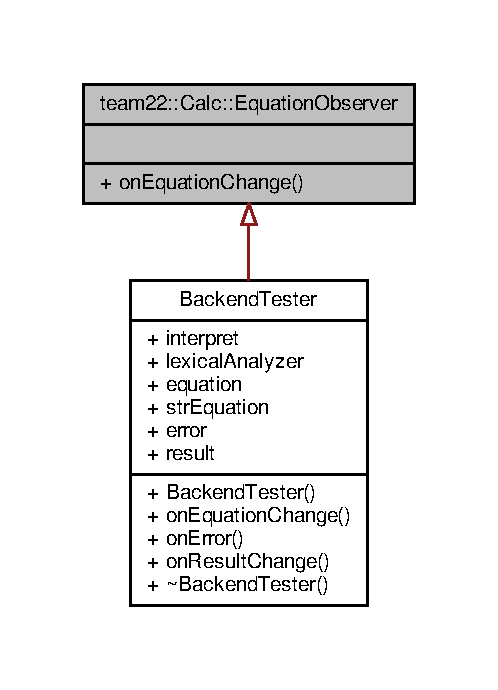
\includegraphics[width=239pt]{classteam22_1_1_calc_1_1_equation_observer__inherit__graph}
\end{center}
\end{figure}


Collaboration diagram for team22\+:\+:Calc\+:\+:Equation\+Observer\+:
\nopagebreak
\begin{figure}[H]
\begin{center}
\leavevmode
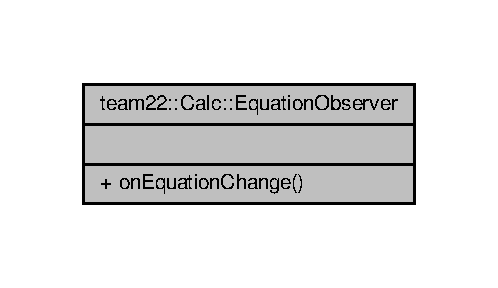
\includegraphics[width=239pt]{classteam22_1_1_calc_1_1_equation_observer__coll__graph}
\end{center}
\end{figure}
\subsection*{Public Member Functions}
\begin{DoxyCompactItemize}
\item 
virtual void \hyperlink{classteam22_1_1_calc_1_1_equation_observer_a2fc2a1f8583f27b0087ff6053895ef25}{on\+Equation\+Change} ()=0
\end{DoxyCompactItemize}


\subsection{Detailed Description}


Definition at line 12 of file Equation\+Observer.\+h.



\subsection{Member Function Documentation}
\mbox{\Hypertarget{classteam22_1_1_calc_1_1_equation_observer_a2fc2a1f8583f27b0087ff6053895ef25}\label{classteam22_1_1_calc_1_1_equation_observer_a2fc2a1f8583f27b0087ff6053895ef25}} 
\index{team22\+::\+Calc\+::\+Equation\+Observer@{team22\+::\+Calc\+::\+Equation\+Observer}!on\+Equation\+Change@{on\+Equation\+Change}}
\index{on\+Equation\+Change@{on\+Equation\+Change}!team22\+::\+Calc\+::\+Equation\+Observer@{team22\+::\+Calc\+::\+Equation\+Observer}}
\subsubsection{\texorpdfstring{on\+Equation\+Change()}{onEquationChange()}}
{\footnotesize\ttfamily virtual void team22\+::\+Calc\+::\+Equation\+Observer\+::on\+Equation\+Change (\begin{DoxyParamCaption}{ }\end{DoxyParamCaption})\hspace{0.3cm}{\ttfamily [pure virtual]}}



Implemented in \hyperlink{class_backend_tester_a9b7caf17f8ad274936fab5ca4bc669f8}{Backend\+Tester}.



The documentation for this class was generated from the following file\+:\begin{DoxyCompactItemize}
\item 
src/\hyperlink{_equation_observer_8h}{Equation\+Observer.\+h}\end{DoxyCompactItemize}

\hypertarget{struct_exp}{}\section{Exp Struct Reference}
\label{struct_exp}\index{Exp@{Exp}}


Inheritance diagram for Exp\+:
\nopagebreak
\begin{figure}[H]
\begin{center}
\leavevmode
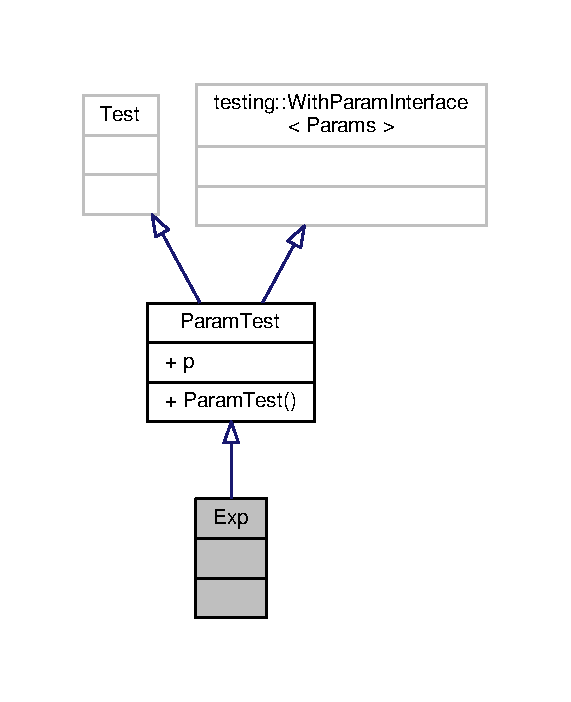
\includegraphics[width=274pt]{struct_exp__inherit__graph}
\end{center}
\end{figure}


Collaboration diagram for Exp\+:
\nopagebreak
\begin{figure}[H]
\begin{center}
\leavevmode
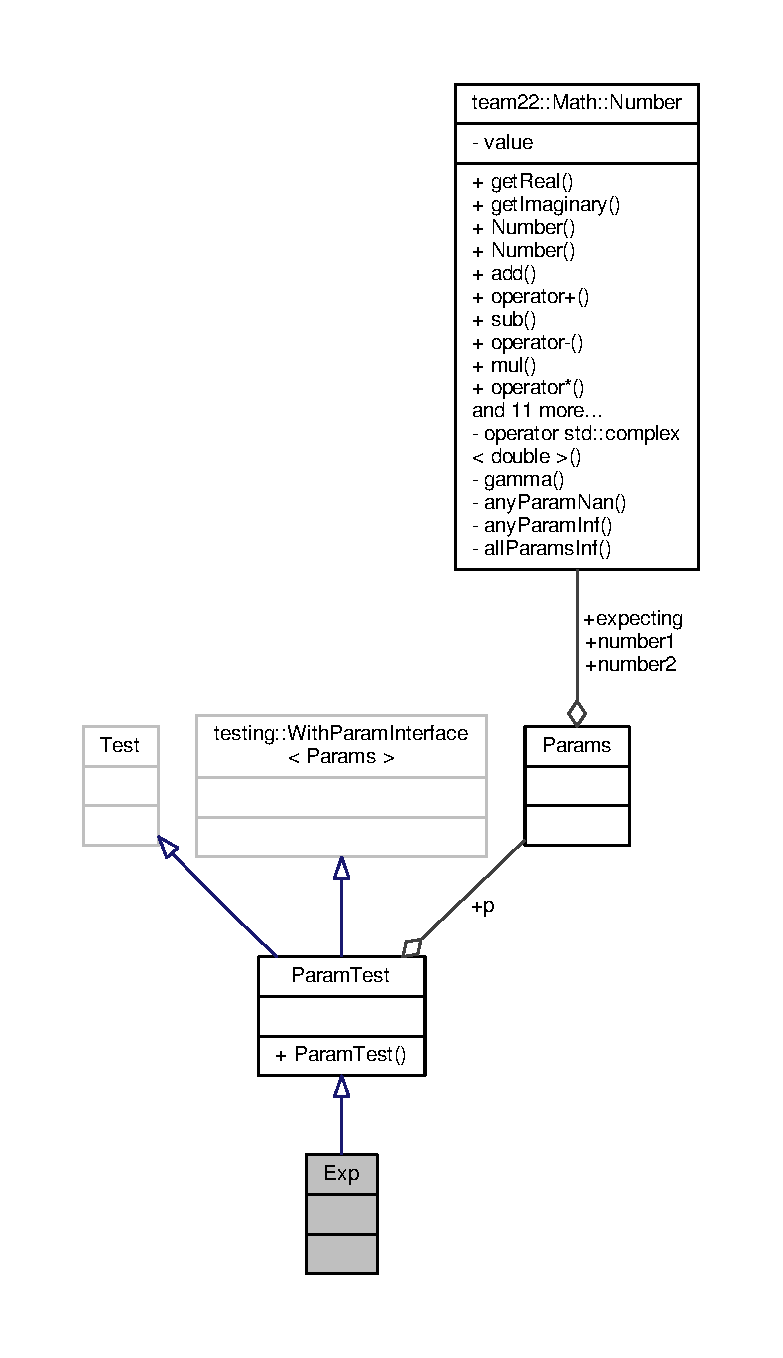
\includegraphics[height=550pt]{struct_exp__coll__graph}
\end{center}
\end{figure}
\subsection*{Additional Inherited Members}


\subsection{Detailed Description}


Definition at line 77 of file Number\+Test.\+cpp.



The documentation for this struct was generated from the following file\+:\begin{DoxyCompactItemize}
\item 
tests/\hyperlink{_number_test_8cpp}{Number\+Test.\+cpp}\end{DoxyCompactItemize}

\hypertarget{struct_factorial}{}\section{Factorial Struct Reference}
\label{struct_factorial}\index{Factorial@{Factorial}}


Inheritance diagram for Factorial\+:
\nopagebreak
\begin{figure}[H]
\begin{center}
\leavevmode
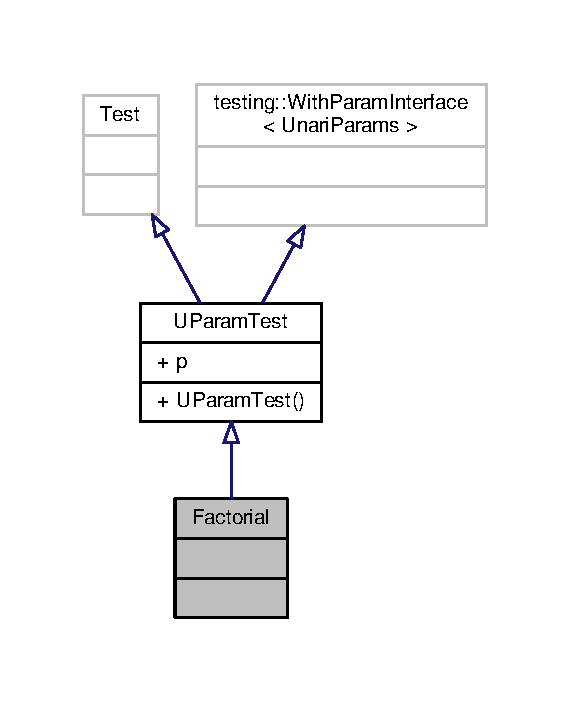
\includegraphics[width=274pt]{struct_factorial__inherit__graph}
\end{center}
\end{figure}


Collaboration diagram for Factorial\+:
\nopagebreak
\begin{figure}[H]
\begin{center}
\leavevmode
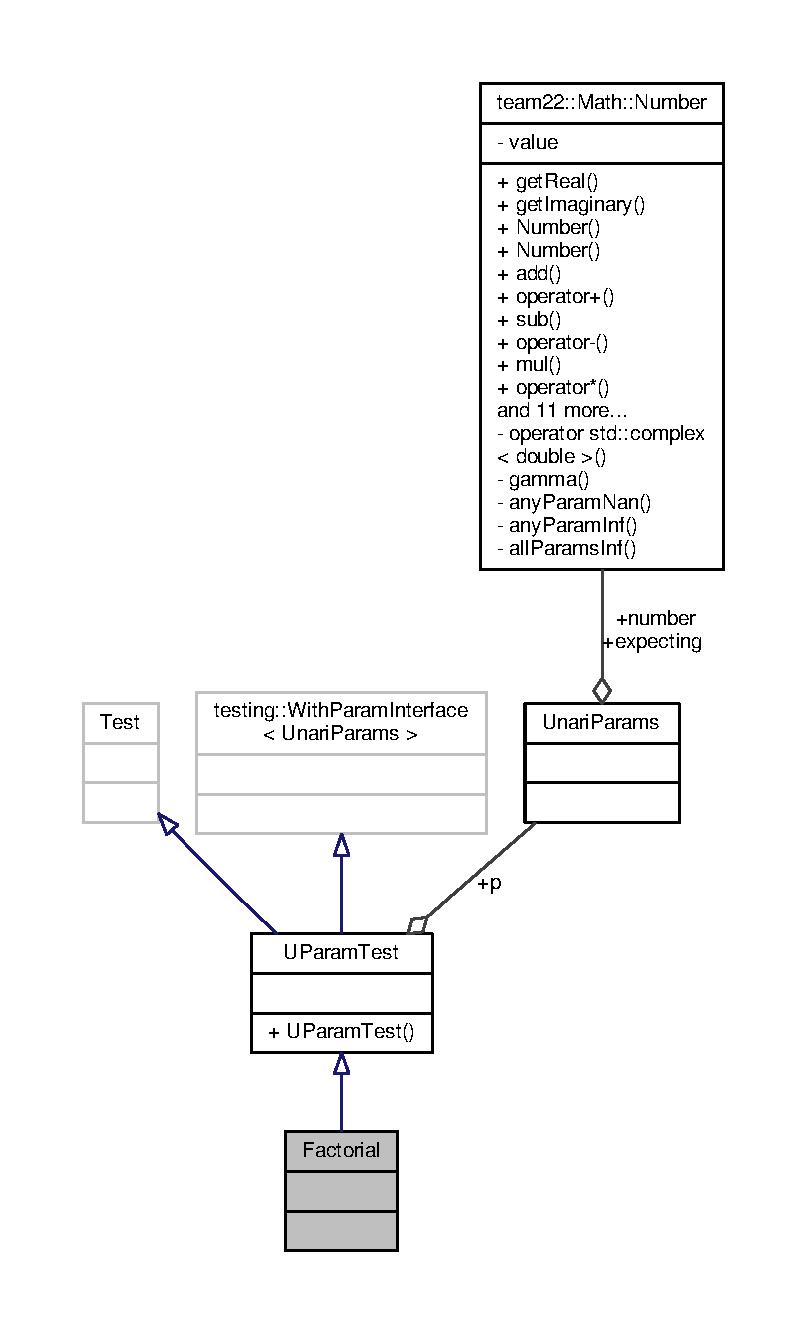
\includegraphics[height=550pt]{struct_factorial__coll__graph}
\end{center}
\end{figure}
\subsection*{Additional Inherited Members}


\subsection{Detailed Description}


Definition at line 80 of file Number\+Test.\+cpp.



The documentation for this struct was generated from the following file\+:\begin{DoxyCompactItemize}
\item 
src/tests/\hyperlink{_number_test_8cpp}{Number\+Test.\+cpp}\end{DoxyCompactItemize}

\hypertarget{classteam22_1_1_calc_1_1_interpret}{}\section{team22\+:\+:Calc\+:\+:Interpret Class Reference}
\label{classteam22_1_1_calc_1_1_interpret}\index{team22\+::\+Calc\+::\+Interpret@{team22\+::\+Calc\+::\+Interpret}}


{\ttfamily \#include $<$Interpret.\+h$>$}



Inheritance diagram for team22\+:\+:Calc\+:\+:Interpret\+:
\nopagebreak
\begin{figure}[H]
\begin{center}
\leavevmode
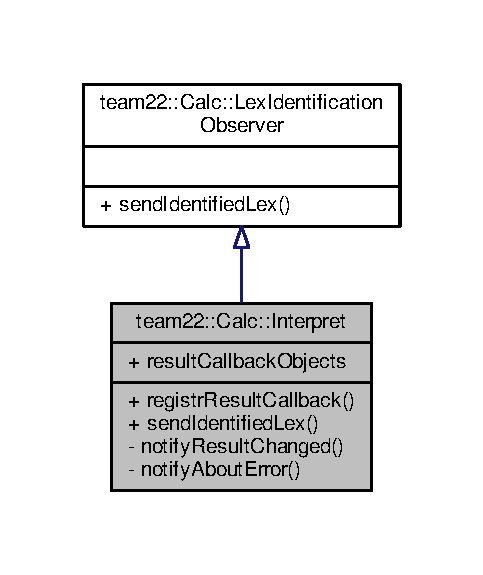
\includegraphics[width=232pt]{classteam22_1_1_calc_1_1_interpret__inherit__graph}
\end{center}
\end{figure}


Collaboration diagram for team22\+:\+:Calc\+:\+:Interpret\+:
\nopagebreak
\begin{figure}[H]
\begin{center}
\leavevmode
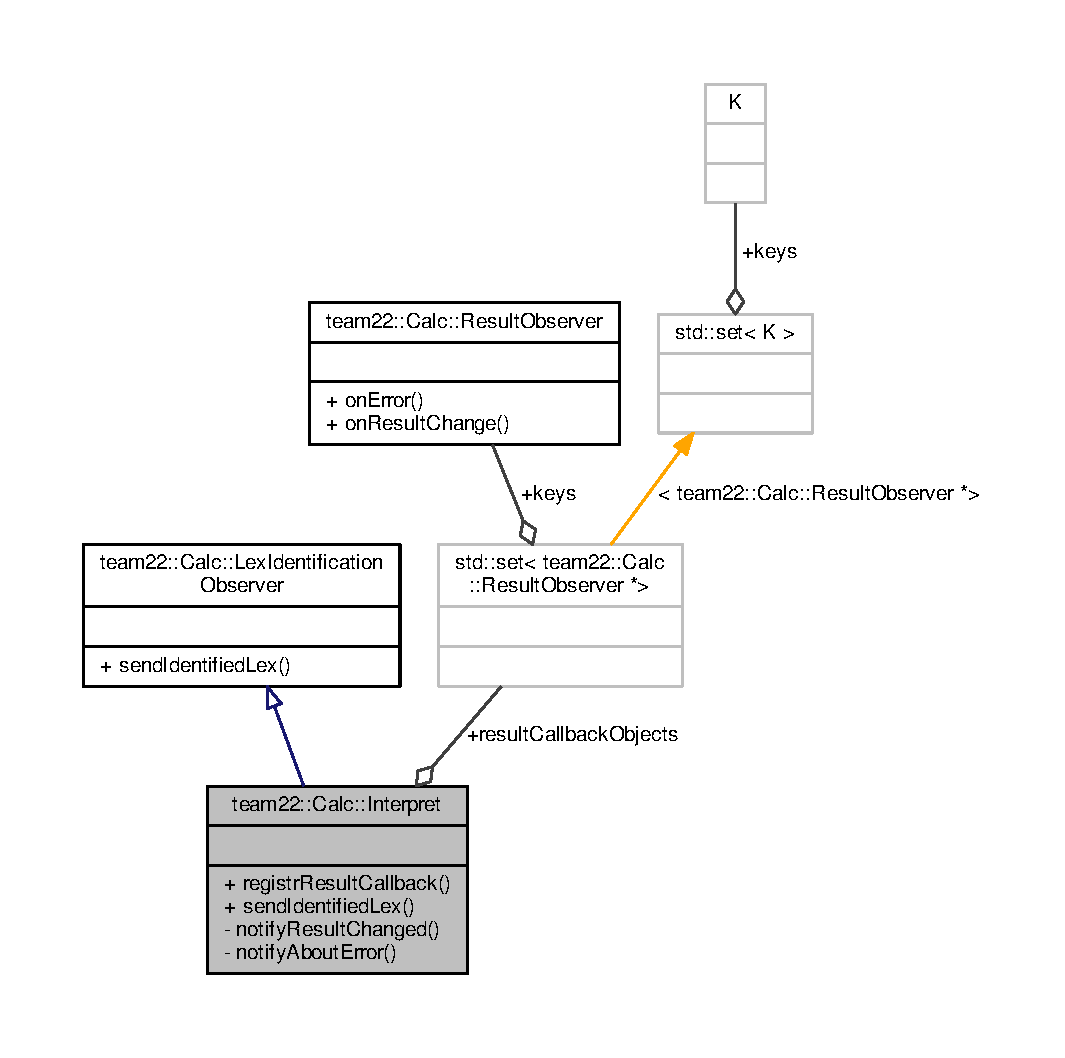
\includegraphics[width=350pt]{classteam22_1_1_calc_1_1_interpret__coll__graph}
\end{center}
\end{figure}
\subsection*{Public Member Functions}
\begin{DoxyCompactItemize}
\item 
void \hyperlink{classteam22_1_1_calc_1_1_interpret_a23e1e307b4f7ffd42f8eb31d33314c41}{registr\+Result\+Callback} (\hyperlink{classteam22_1_1_calc_1_1_result_observer}{Result\+Observer} $\ast$result\+Callback\+Object)
\item 
void \hyperlink{classteam22_1_1_calc_1_1_interpret_a479c65c010f4ef1060049b684e5f7eb6}{send\+Identified\+Lex} (\hyperlink{classteam22_1_1_calc_1_1_lex}{Lex} lex) override
\end{DoxyCompactItemize}
\subsection*{Public Attributes}
\begin{DoxyCompactItemize}
\item 
std\+::set$<$ \hyperlink{classteam22_1_1_calc_1_1_result_observer}{Result\+Observer} $\ast$ $>$ \hyperlink{classteam22_1_1_calc_1_1_interpret_a7db1e80a4733124ed425e62a90f9eadb}{result\+Callback\+Objects}
\end{DoxyCompactItemize}
\subsection*{Private Member Functions}
\begin{DoxyCompactItemize}
\item 
void \hyperlink{classteam22_1_1_calc_1_1_interpret_af38e3b867c32f50c921027249fc1185a}{notify\+Result\+Changed} ()
\item 
void \hyperlink{classteam22_1_1_calc_1_1_interpret_ab9db5790b1aab8a3f315296853c8e9c6}{notify\+About\+Error} (\hyperlink{class_interpret_exception}{Interpret\+Exception} exception)
\end{DoxyCompactItemize}


\subsection{Detailed Description}


Definition at line 48 of file Interpret.\+h.



\subsection{Member Function Documentation}
\mbox{\Hypertarget{classteam22_1_1_calc_1_1_interpret_ab9db5790b1aab8a3f315296853c8e9c6}\label{classteam22_1_1_calc_1_1_interpret_ab9db5790b1aab8a3f315296853c8e9c6}} 
\index{team22\+::\+Calc\+::\+Interpret@{team22\+::\+Calc\+::\+Interpret}!notify\+About\+Error@{notify\+About\+Error}}
\index{notify\+About\+Error@{notify\+About\+Error}!team22\+::\+Calc\+::\+Interpret@{team22\+::\+Calc\+::\+Interpret}}
\subsubsection{\texorpdfstring{notify\+About\+Error()}{notifyAboutError()}}
{\footnotesize\ttfamily void Interpret\+::notify\+About\+Error (\begin{DoxyParamCaption}\item[{\hyperlink{class_interpret_exception}{Interpret\+Exception}}]{exception }\end{DoxyParamCaption})\hspace{0.3cm}{\ttfamily [private]}}

Předá informaci o změně výsledků pozorovatelům \begin{Desc}
\item[Examples\+: ]\par
\hyperlink{_2root_2_documents_2_git_clone_2_f_i_t__i_v_s__p_r_o_j_e_c_t2_2src_2_interpret_8h-example}{/root/\+Documents/\+Git\+Clone/\+F\+I\+T\+\_\+\+I\+V\+S\+\_\+\+P\+R\+O\+J\+E\+C\+T2/src/\+Interpret.\+h}.\end{Desc}


Definition at line 28 of file Interpret.\+cpp.



References result\+Callback\+Objects.

\mbox{\Hypertarget{classteam22_1_1_calc_1_1_interpret_af38e3b867c32f50c921027249fc1185a}\label{classteam22_1_1_calc_1_1_interpret_af38e3b867c32f50c921027249fc1185a}} 
\index{team22\+::\+Calc\+::\+Interpret@{team22\+::\+Calc\+::\+Interpret}!notify\+Result\+Changed@{notify\+Result\+Changed}}
\index{notify\+Result\+Changed@{notify\+Result\+Changed}!team22\+::\+Calc\+::\+Interpret@{team22\+::\+Calc\+::\+Interpret}}
\subsubsection{\texorpdfstring{notify\+Result\+Changed()}{notifyResultChanged()}}
{\footnotesize\ttfamily void Interpret\+::notify\+Result\+Changed (\begin{DoxyParamCaption}{ }\end{DoxyParamCaption})\hspace{0.3cm}{\ttfamily [private]}}

Předá informaci o změně výsledků pozorovatelům \begin{Desc}
\item[Examples\+: ]\par
\hyperlink{_2root_2_documents_2_git_clone_2_f_i_t__i_v_s__p_r_o_j_e_c_t2_2src_2_interpret_8h-example}{/root/\+Documents/\+Git\+Clone/\+F\+I\+T\+\_\+\+I\+V\+S\+\_\+\+P\+R\+O\+J\+E\+C\+T2/src/\+Interpret.\+h}.\end{Desc}


Definition at line 22 of file Interpret.\+cpp.



References result\+Callback\+Objects.

\mbox{\Hypertarget{classteam22_1_1_calc_1_1_interpret_a23e1e307b4f7ffd42f8eb31d33314c41}\label{classteam22_1_1_calc_1_1_interpret_a23e1e307b4f7ffd42f8eb31d33314c41}} 
\index{team22\+::\+Calc\+::\+Interpret@{team22\+::\+Calc\+::\+Interpret}!registr\+Result\+Callback@{registr\+Result\+Callback}}
\index{registr\+Result\+Callback@{registr\+Result\+Callback}!team22\+::\+Calc\+::\+Interpret@{team22\+::\+Calc\+::\+Interpret}}
\subsubsection{\texorpdfstring{registr\+Result\+Callback()}{registrResultCallback()}}
{\footnotesize\ttfamily void Interpret\+::registr\+Result\+Callback (\begin{DoxyParamCaption}\item[{\hyperlink{classteam22_1_1_calc_1_1_result_observer}{Result\+Observer} $\ast$}]{result\+Callback\+Object }\end{DoxyParamCaption})}

Registruje objekt k odběru rozeznaných lexémů vícenásobná registrace stejné instance odběratele neprovede nic


\begin{DoxyParams}{Parameters}
{\em result\+Callback\+Object} & objekt na němž bude volán callback při změně výsledku nebo chybě \\
\hline
\end{DoxyParams}
\begin{Desc}
\item[Examples\+: ]\par
\hyperlink{_2root_2_documents_2_git_clone_2_f_i_t__i_v_s__p_r_o_j_e_c_t2_2src_2_interpret_8h-example}{/root/\+Documents/\+Git\+Clone/\+F\+I\+T\+\_\+\+I\+V\+S\+\_\+\+P\+R\+O\+J\+E\+C\+T2/src/\+Interpret.\+h}.\end{Desc}


Definition at line 17 of file Interpret.\+cpp.



References result\+Callback\+Objects.



Referenced by Backend\+Tester\+::\+Backend\+Tester(), and Interpret\+Test\+::\+Interpret\+Test().

\mbox{\Hypertarget{classteam22_1_1_calc_1_1_interpret_a479c65c010f4ef1060049b684e5f7eb6}\label{classteam22_1_1_calc_1_1_interpret_a479c65c010f4ef1060049b684e5f7eb6}} 
\index{team22\+::\+Calc\+::\+Interpret@{team22\+::\+Calc\+::\+Interpret}!send\+Identified\+Lex@{send\+Identified\+Lex}}
\index{send\+Identified\+Lex@{send\+Identified\+Lex}!team22\+::\+Calc\+::\+Interpret@{team22\+::\+Calc\+::\+Interpret}}
\subsubsection{\texorpdfstring{send\+Identified\+Lex()}{sendIdentifiedLex()}}
{\footnotesize\ttfamily void Interpret\+::send\+Identified\+Lex (\begin{DoxyParamCaption}\item[{\hyperlink{classteam22_1_1_calc_1_1_lex}{Lex}}]{lex }\end{DoxyParamCaption})\hspace{0.3cm}{\ttfamily [override]}, {\ttfamily [virtual]}}

Příjme lexém k interpretaci \begin{DoxySeeAlso}{See also}
\hyperlink{classteam22_1_1_calc_1_1_interpret}{Interpret} popis postupu interpretace 
\end{DoxySeeAlso}

\begin{DoxyParams}{Parameters}
{\em lex} & \\
\hline
\end{DoxyParams}


Implements \hyperlink{classteam22_1_1_calc_1_1_lex_identification_observer_ac139f75c560625ec6fdb2e34cf0d4884}{team22\+::\+Calc\+::\+Lex\+Identification\+Observer}.

\begin{Desc}
\item[Examples\+: ]\par
\hyperlink{_2root_2_documents_2_git_clone_2_f_i_t__i_v_s__p_r_o_j_e_c_t2_2src_2_interpret_8h-example}{/root/\+Documents/\+Git\+Clone/\+F\+I\+T\+\_\+\+I\+V\+S\+\_\+\+P\+R\+O\+J\+E\+C\+T2/src/\+Interpret.\+h}.\end{Desc}


Definition at line 12 of file Interpret.\+cpp.



Referenced by team22\+::\+Calc\+::\+Equation\+::re\+Compute\+Result(), and team22\+::\+Calc\+::\+Equation\+::send\+Identified\+Lex().



\subsection{Member Data Documentation}
\mbox{\Hypertarget{classteam22_1_1_calc_1_1_interpret_a7db1e80a4733124ed425e62a90f9eadb}\label{classteam22_1_1_calc_1_1_interpret_a7db1e80a4733124ed425e62a90f9eadb}} 
\index{team22\+::\+Calc\+::\+Interpret@{team22\+::\+Calc\+::\+Interpret}!result\+Callback\+Objects@{result\+Callback\+Objects}}
\index{result\+Callback\+Objects@{result\+Callback\+Objects}!team22\+::\+Calc\+::\+Interpret@{team22\+::\+Calc\+::\+Interpret}}
\subsubsection{\texorpdfstring{result\+Callback\+Objects}{resultCallbackObjects}}
{\footnotesize\ttfamily std\+::set$<$\hyperlink{classteam22_1_1_calc_1_1_result_observer}{Result\+Observer} $\ast$$>$ team22\+::\+Calc\+::\+Interpret\+::result\+Callback\+Objects}

Množina Objektů na nichž bude volán callback při změně výsledku nebo chybě \begin{Desc}
\item[Examples\+: ]\par
\hyperlink{_2root_2_documents_2_git_clone_2_f_i_t__i_v_s__p_r_o_j_e_c_t2_2src_2_interpret_8h-example}{/root/\+Documents/\+Git\+Clone/\+F\+I\+T\+\_\+\+I\+V\+S\+\_\+\+P\+R\+O\+J\+E\+C\+T2/src/\+Interpret.\+h}.\end{Desc}


Definition at line 64 of file Interpret.\+h.



Referenced by notify\+About\+Error(), notify\+Result\+Changed(), and registr\+Result\+Callback().



The documentation for this class was generated from the following files\+:\begin{DoxyCompactItemize}
\item 
src/\hyperlink{_interpret_8h}{Interpret.\+h}\item 
src/\hyperlink{_interpret_8cpp}{Interpret.\+cpp}\end{DoxyCompactItemize}

\hypertarget{class_interpret_exception}{}\section{Interpret\+Exception Class Reference}
\label{class_interpret_exception}\index{Interpret\+Exception@{Interpret\+Exception}}


{\ttfamily \#include $<$Interpret\+Exception.\+h$>$}



Collaboration diagram for Interpret\+Exception\+:
\nopagebreak
\begin{figure}[H]
\begin{center}
\leavevmode
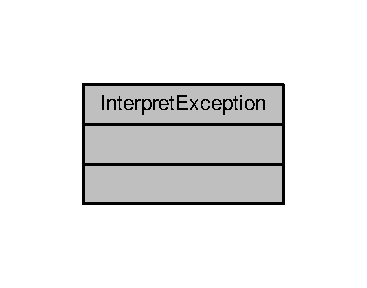
\includegraphics[width=176pt]{class_interpret_exception__coll__graph}
\end{center}
\end{figure}


\subsection{Detailed Description}
\begin{Desc}
\item[Examples\+: ]\par
\hyperlink{_2root_2_documents_2_git_clone_2_f_i_t__i_v_s__p_r_o_j_e_c_t2_2src_2_interpret_8h-example}{/root/\+Documents/\+Git\+Clone/\+F\+I\+T\+\_\+\+I\+V\+S\+\_\+\+P\+R\+O\+J\+E\+C\+T2/src/\+Interpret.\+h}.\end{Desc}


Definition at line 11 of file Interpret\+Exception.\+h.



The documentation for this class was generated from the following file\+:\begin{DoxyCompactItemize}
\item 
src/\hyperlink{_interpret_exception_8h}{Interpret\+Exception.\+h}\end{DoxyCompactItemize}

\hypertarget{struct_interpret_test}{}\section{Interpret\+Test Struct Reference}
\label{struct_interpret_test}\index{Interpret\+Test@{Interpret\+Test}}


Inheritance diagram for Interpret\+Test\+:
\nopagebreak
\begin{figure}[H]
\begin{center}
\leavevmode
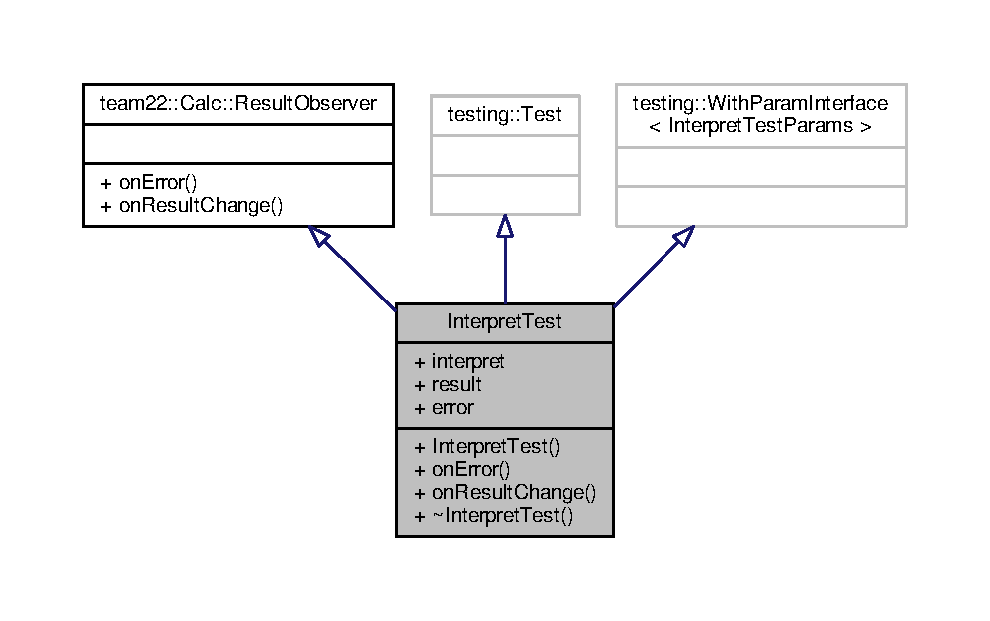
\includegraphics[width=350pt]{struct_interpret_test__inherit__graph}
\end{center}
\end{figure}


Collaboration diagram for Interpret\+Test\+:
\nopagebreak
\begin{figure}[H]
\begin{center}
\leavevmode
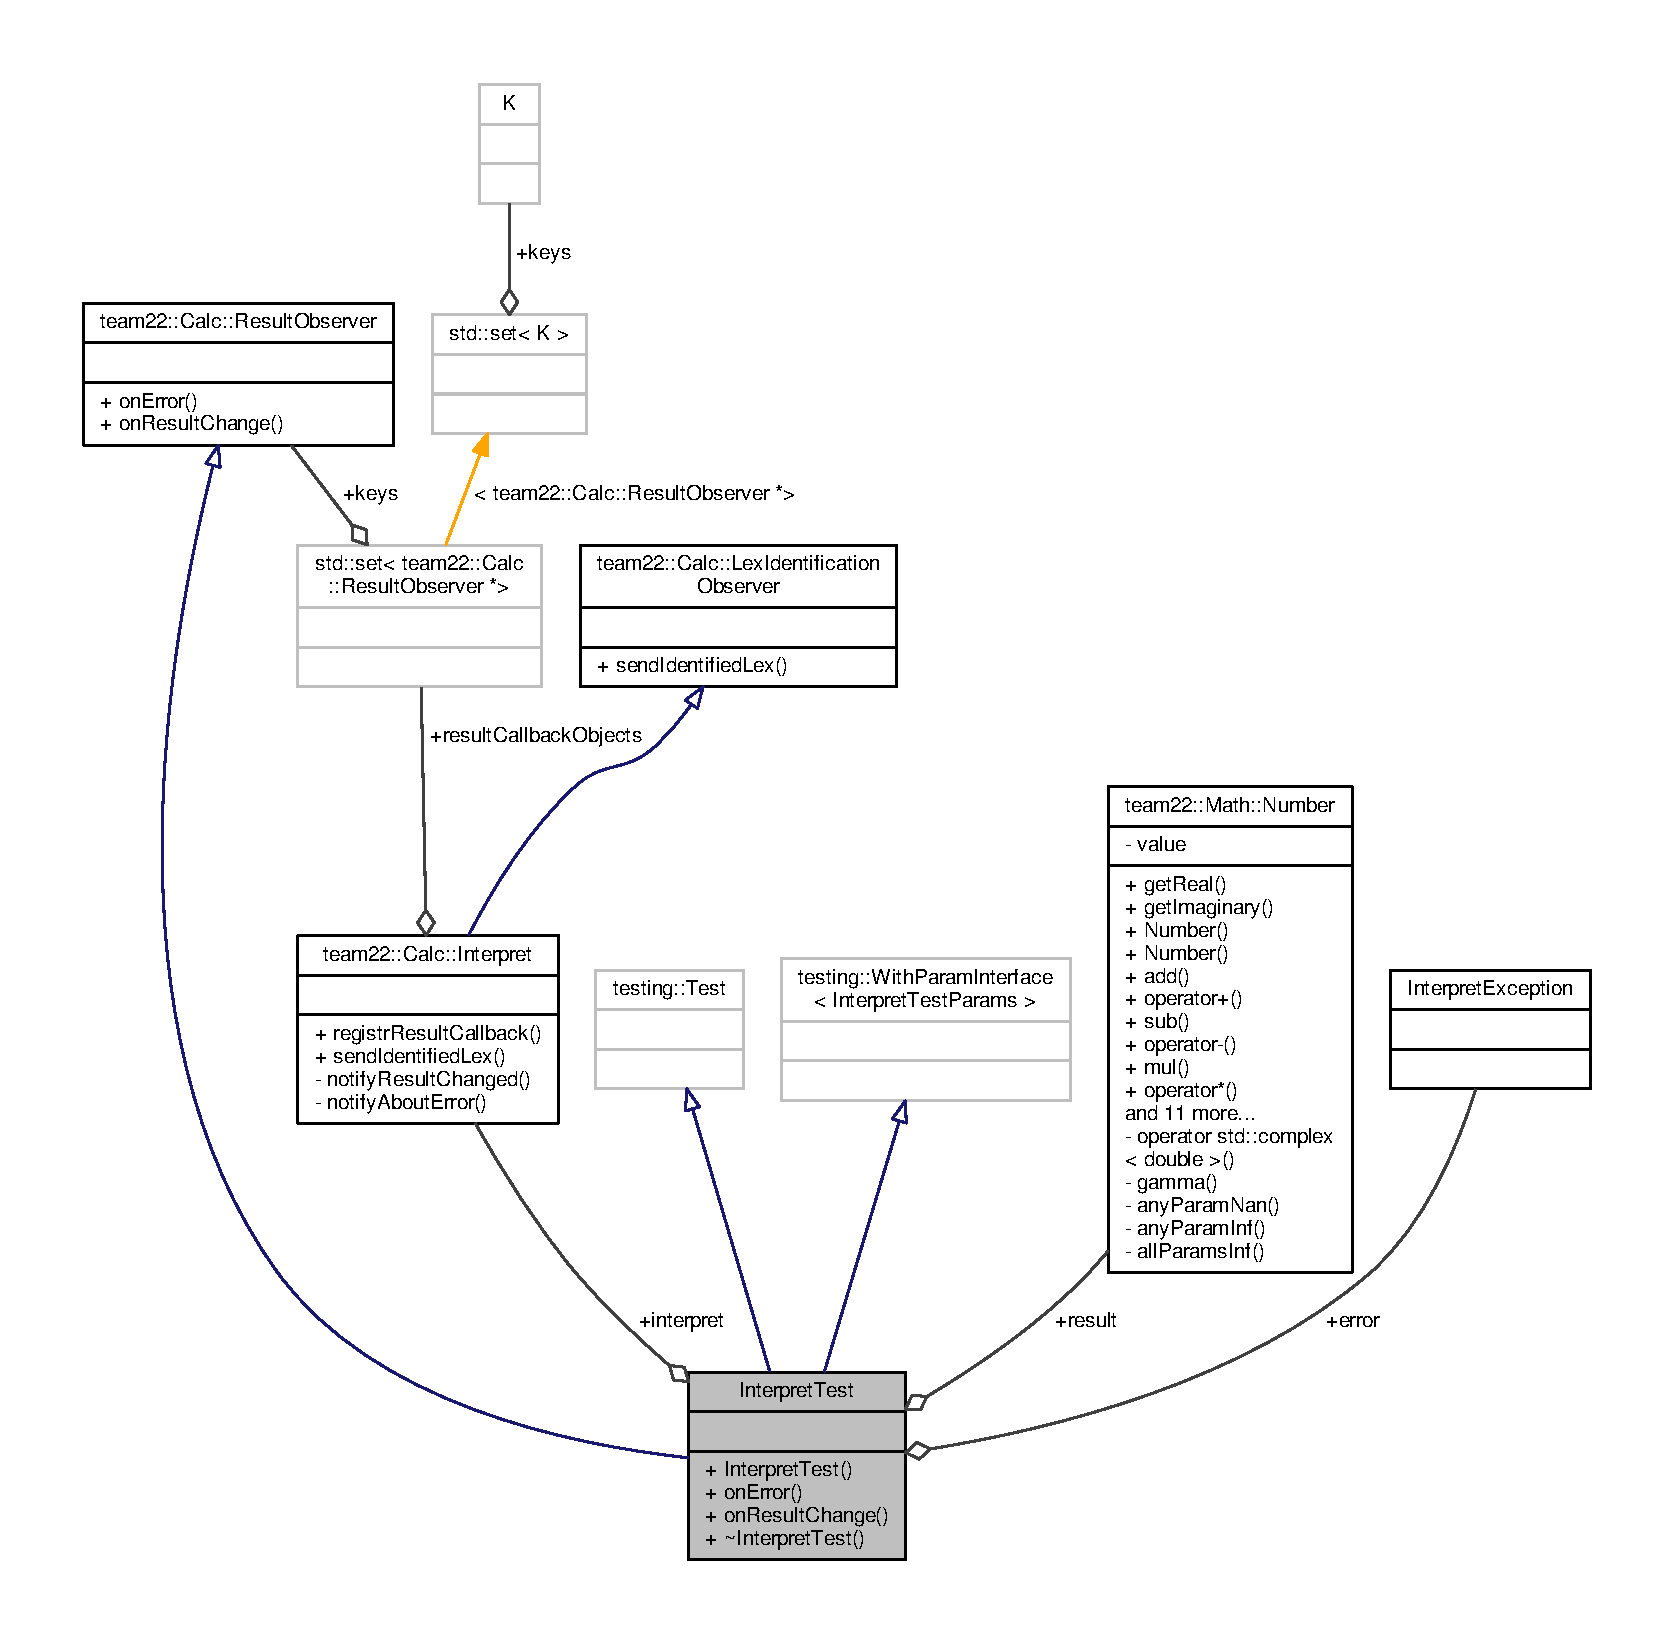
\includegraphics[width=350pt]{struct_interpret_test__coll__graph}
\end{center}
\end{figure}
\subsection*{Public Member Functions}
\begin{DoxyCompactItemize}
\item 
\hyperlink{struct_interpret_test_af1827c5b47519fbc03c10a7ed1591d44}{Interpret\+Test} ()
\item 
void \hyperlink{struct_interpret_test_a8dd2550d1b3e604db0230c2a3f4807a5}{on\+Error} (\hyperlink{class_interpret_exception}{Interpret\+Exception} exception) override
\item 
void \hyperlink{struct_interpret_test_af3c7dfecc5779919bf629c558c696548}{on\+Result\+Change} (\hyperlink{classteam22_1_1_math_1_1_number}{Number} \hyperlink{struct_interpret_test_a8a1290387dfa72192d3ea06873ff8e73}{result}) override
\item 
virtual \hyperlink{struct_interpret_test_abd93b9443a1b18087a2c879e7664af00}{$\sim$\+Interpret\+Test} ()
\end{DoxyCompactItemize}
\subsection*{Public Attributes}
\begin{DoxyCompactItemize}
\item 
\hyperlink{classteam22_1_1_calc_1_1_interpret}{Interpret} \hyperlink{struct_interpret_test_a3905fe89984120323e1dd28b2abd6052}{interpret}
\item 
\hyperlink{classteam22_1_1_math_1_1_number}{Number} \hyperlink{struct_interpret_test_a8a1290387dfa72192d3ea06873ff8e73}{result} = \{0\}
\item 
\hyperlink{class_interpret_exception}{Interpret\+Exception} $\ast$ \hyperlink{struct_interpret_test_aace2257ef8c92219d240f5e2e430bd2b}{error} = nullptr
\end{DoxyCompactItemize}


\subsection{Detailed Description}


Definition at line 38 of file Interpret\+Tests.\+cpp.



\subsection{Constructor \& Destructor Documentation}
\mbox{\Hypertarget{struct_interpret_test_af1827c5b47519fbc03c10a7ed1591d44}\label{struct_interpret_test_af1827c5b47519fbc03c10a7ed1591d44}} 
\index{Interpret\+Test@{Interpret\+Test}!Interpret\+Test@{Interpret\+Test}}
\index{Interpret\+Test@{Interpret\+Test}!Interpret\+Test@{Interpret\+Test}}
\subsubsection{\texorpdfstring{Interpret\+Test()}{InterpretTest()}}
{\footnotesize\ttfamily Interpret\+Test\+::\+Interpret\+Test (\begin{DoxyParamCaption}{ }\end{DoxyParamCaption})\hspace{0.3cm}{\ttfamily [inline]}}



Definition at line 47 of file Interpret\+Tests.\+cpp.



References team22\+::\+Calc\+::\+Interpret\+::registr\+Result\+Callback().

\mbox{\Hypertarget{struct_interpret_test_abd93b9443a1b18087a2c879e7664af00}\label{struct_interpret_test_abd93b9443a1b18087a2c879e7664af00}} 
\index{Interpret\+Test@{Interpret\+Test}!````~Interpret\+Test@{$\sim$\+Interpret\+Test}}
\index{````~Interpret\+Test@{$\sim$\+Interpret\+Test}!Interpret\+Test@{Interpret\+Test}}
\subsubsection{\texorpdfstring{$\sim$\+Interpret\+Test()}{~InterpretTest()}}
{\footnotesize\ttfamily virtual Interpret\+Test\+::$\sim$\+Interpret\+Test (\begin{DoxyParamCaption}{ }\end{DoxyParamCaption})\hspace{0.3cm}{\ttfamily [inline]}, {\ttfamily [virtual]}}



Definition at line 62 of file Interpret\+Tests.\+cpp.



References team22\+::\+Calc\+::\+Lex\+::\+A\+DD, team22\+::\+Calc\+::\+Lex\+::\+BS, team22\+::\+Calc\+::\+Lex\+::\+C\+L\+E\+AR, team22\+::\+Calc\+::\+Lex\+::\+D\+IV, team22\+::\+Calc\+::\+Lex\+::\+E\+V\+AL, team22\+::\+Calc\+::\+Lex\+::\+E\+XP, team22\+::\+Calc\+::\+Lex\+::\+F\+A\+C\+T\+O\+R\+I\+AL, I\+N\+S\+T\+A\+N\+T\+I\+A\+T\+E\+\_\+\+T\+E\+S\+T\+\_\+\+C\+A\+S\+E\+\_\+\+P(), team22\+::\+Calc\+::\+Lex\+::\+M\+OD, team22\+::\+Calc\+::\+Lex\+::\+M\+UL, team22\+::\+Calc\+::\+Lex\+::\+R\+O\+OT, and team22\+::\+Calc\+::\+Lex\+::\+S\+UB.



\subsection{Member Function Documentation}
\mbox{\Hypertarget{struct_interpret_test_a8dd2550d1b3e604db0230c2a3f4807a5}\label{struct_interpret_test_a8dd2550d1b3e604db0230c2a3f4807a5}} 
\index{Interpret\+Test@{Interpret\+Test}!on\+Error@{on\+Error}}
\index{on\+Error@{on\+Error}!Interpret\+Test@{Interpret\+Test}}
\subsubsection{\texorpdfstring{on\+Error()}{onError()}}
{\footnotesize\ttfamily void Interpret\+Test\+::on\+Error (\begin{DoxyParamCaption}\item[{\hyperlink{class_interpret_exception}{Interpret\+Exception}}]{exception }\end{DoxyParamCaption})\hspace{0.3cm}{\ttfamily [inline]}, {\ttfamily [override]}, {\ttfamily [virtual]}}

Callback volaný pokud vznikla chyba při výpočtu 
\begin{DoxyParams}{Parameters}
{\em \hyperlink{class_interpret_exception}{Interpret\+Exception}} & \\
\hline
\end{DoxyParams}


Implements \hyperlink{classteam22_1_1_calc_1_1_result_observer_ad36cf8df89853d60f91094800c01d329}{team22\+::\+Calc\+::\+Result\+Observer}.



Definition at line 52 of file Interpret\+Tests.\+cpp.

\mbox{\Hypertarget{struct_interpret_test_af3c7dfecc5779919bf629c558c696548}\label{struct_interpret_test_af3c7dfecc5779919bf629c558c696548}} 
\index{Interpret\+Test@{Interpret\+Test}!on\+Result\+Change@{on\+Result\+Change}}
\index{on\+Result\+Change@{on\+Result\+Change}!Interpret\+Test@{Interpret\+Test}}
\subsubsection{\texorpdfstring{on\+Result\+Change()}{onResultChange()}}
{\footnotesize\ttfamily void Interpret\+Test\+::on\+Result\+Change (\begin{DoxyParamCaption}\item[{\hyperlink{classteam22_1_1_math_1_1_number}{Number}}]{result }\end{DoxyParamCaption})\hspace{0.3cm}{\ttfamily [inline]}, {\ttfamily [override]}, {\ttfamily [virtual]}}

Callback volaný při změně výsledku 
\begin{DoxyParams}{Parameters}
{\em result} & \\
\hline
\end{DoxyParams}


Implements \hyperlink{classteam22_1_1_calc_1_1_result_observer_aa04007df3aa8a499c3a511f549238285}{team22\+::\+Calc\+::\+Result\+Observer}.



Definition at line 57 of file Interpret\+Tests.\+cpp.



\subsection{Member Data Documentation}
\mbox{\Hypertarget{struct_interpret_test_aace2257ef8c92219d240f5e2e430bd2b}\label{struct_interpret_test_aace2257ef8c92219d240f5e2e430bd2b}} 
\index{Interpret\+Test@{Interpret\+Test}!error@{error}}
\index{error@{error}!Interpret\+Test@{Interpret\+Test}}
\subsubsection{\texorpdfstring{error}{error}}
{\footnotesize\ttfamily \hyperlink{class_interpret_exception}{Interpret\+Exception}$\ast$ Interpret\+Test\+::error = nullptr}



Definition at line 45 of file Interpret\+Tests.\+cpp.

\mbox{\Hypertarget{struct_interpret_test_a3905fe89984120323e1dd28b2abd6052}\label{struct_interpret_test_a3905fe89984120323e1dd28b2abd6052}} 
\index{Interpret\+Test@{Interpret\+Test}!interpret@{interpret}}
\index{interpret@{interpret}!Interpret\+Test@{Interpret\+Test}}
\subsubsection{\texorpdfstring{interpret}{interpret}}
{\footnotesize\ttfamily \hyperlink{classteam22_1_1_calc_1_1_interpret}{Interpret} Interpret\+Test\+::interpret}



Definition at line 43 of file Interpret\+Tests.\+cpp.

\mbox{\Hypertarget{struct_interpret_test_a8a1290387dfa72192d3ea06873ff8e73}\label{struct_interpret_test_a8a1290387dfa72192d3ea06873ff8e73}} 
\index{Interpret\+Test@{Interpret\+Test}!result@{result}}
\index{result@{result}!Interpret\+Test@{Interpret\+Test}}
\subsubsection{\texorpdfstring{result}{result}}
{\footnotesize\ttfamily \hyperlink{classteam22_1_1_math_1_1_number}{Number} Interpret\+Test\+::result = \{0\}}



Definition at line 44 of file Interpret\+Tests.\+cpp.



The documentation for this struct was generated from the following file\+:\begin{DoxyCompactItemize}
\item 
src/tests/\hyperlink{_interpret_tests_8cpp}{Interpret\+Tests.\+cpp}\end{DoxyCompactItemize}

\hypertarget{struct_interpret_test_params}{}\section{Interpret\+Test\+Params Struct Reference}
\label{struct_interpret_test_params}\index{Interpret\+Test\+Params@{Interpret\+Test\+Params}}


Collaboration diagram for Interpret\+Test\+Params\+:
\nopagebreak
\begin{figure}[H]
\begin{center}
\leavevmode
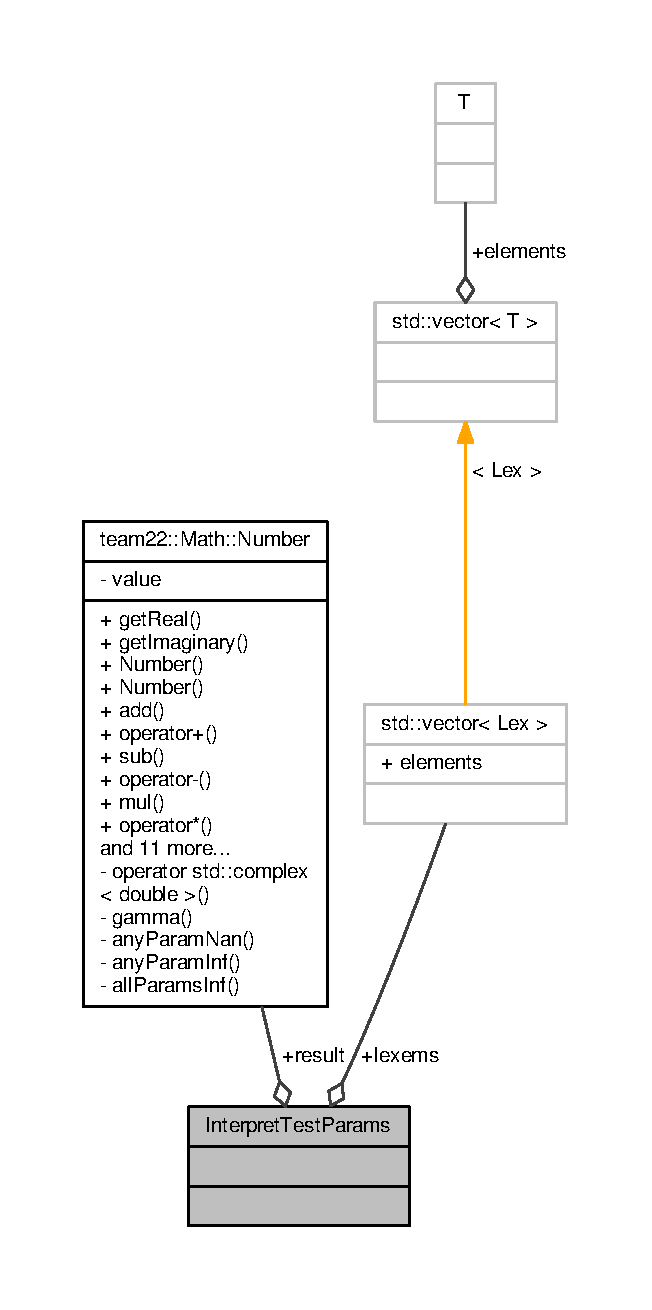
\includegraphics[height=550pt]{struct_interpret_test_params__coll__graph}
\end{center}
\end{figure}
\subsection*{Public Attributes}
\begin{DoxyCompactItemize}
\item 
vector$<$ \hyperlink{classteam22_1_1_calc_1_1_lex}{Lex} $>$ \hyperlink{struct_interpret_test_params_a3e6aa774e846f241efaa2edf7de601b6}{lexems}
\item 
\hyperlink{classteam22_1_1_math_1_1_number}{Number} \hyperlink{struct_interpret_test_params_a47453b7066c4a8ffa209157af91e7ae7}{result}
\end{DoxyCompactItemize}
\subsection*{Friends}
\begin{DoxyCompactItemize}
\item 
std\+::ostream \& \hyperlink{struct_interpret_test_params_a0f38144fe48e0672e466f59fea17dfc2}{operator$<$$<$} (std\+::ostream \&os, const \hyperlink{struct_interpret_test_params}{Interpret\+Test\+Params} \&params)
\end{DoxyCompactItemize}


\subsection{Detailed Description}


Definition at line 19 of file Interpret\+Tests.\+cpp.



\subsection{Friends And Related Function Documentation}
\mbox{\Hypertarget{struct_interpret_test_params_a0f38144fe48e0672e466f59fea17dfc2}\label{struct_interpret_test_params_a0f38144fe48e0672e466f59fea17dfc2}} 
\index{Interpret\+Test\+Params@{Interpret\+Test\+Params}!operator$<$$<$@{operator$<$$<$}}
\index{operator$<$$<$@{operator$<$$<$}!Interpret\+Test\+Params@{Interpret\+Test\+Params}}
\subsubsection{\texorpdfstring{operator$<$$<$}{operator<<}}
{\footnotesize\ttfamily std\+::ostream\& operator$<$$<$ (\begin{DoxyParamCaption}\item[{std\+::ostream \&}]{os,  }\item[{const \hyperlink{struct_interpret_test_params}{Interpret\+Test\+Params} \&}]{params }\end{DoxyParamCaption})\hspace{0.3cm}{\ttfamily [friend]}}



Definition at line 24 of file Interpret\+Tests.\+cpp.



\subsection{Member Data Documentation}
\mbox{\Hypertarget{struct_interpret_test_params_a3e6aa774e846f241efaa2edf7de601b6}\label{struct_interpret_test_params_a3e6aa774e846f241efaa2edf7de601b6}} 
\index{Interpret\+Test\+Params@{Interpret\+Test\+Params}!lexems@{lexems}}
\index{lexems@{lexems}!Interpret\+Test\+Params@{Interpret\+Test\+Params}}
\subsubsection{\texorpdfstring{lexems}{lexems}}
{\footnotesize\ttfamily vector$<$\hyperlink{classteam22_1_1_calc_1_1_lex}{Lex}$>$ Interpret\+Test\+Params\+::lexems}



Definition at line 21 of file Interpret\+Tests.\+cpp.

\mbox{\Hypertarget{struct_interpret_test_params_a47453b7066c4a8ffa209157af91e7ae7}\label{struct_interpret_test_params_a47453b7066c4a8ffa209157af91e7ae7}} 
\index{Interpret\+Test\+Params@{Interpret\+Test\+Params}!result@{result}}
\index{result@{result}!Interpret\+Test\+Params@{Interpret\+Test\+Params}}
\subsubsection{\texorpdfstring{result}{result}}
{\footnotesize\ttfamily \hyperlink{classteam22_1_1_math_1_1_number}{Number} Interpret\+Test\+Params\+::result}



Definition at line 22 of file Interpret\+Tests.\+cpp.



The documentation for this struct was generated from the following file\+:\begin{DoxyCompactItemize}
\item 
src/tests/\hyperlink{_interpret_tests_8cpp}{Interpret\+Tests.\+cpp}\end{DoxyCompactItemize}

\hypertarget{classteam22_1_1_calc_1_1_lex}{}\section{team22\+:\+:Calc\+:\+:Lex Class Reference}
\label{classteam22_1_1_calc_1_1_lex}\index{team22\+::\+Calc\+::\+Lex@{team22\+::\+Calc\+::\+Lex}}


Reprezentace lexému kalkulačky tedy čísla nebo operace.  




{\ttfamily \#include $<$Lex.\+h$>$}



Collaboration diagram for team22\+:\+:Calc\+:\+:Lex\+:
\nopagebreak
\begin{figure}[H]
\begin{center}
\leavevmode
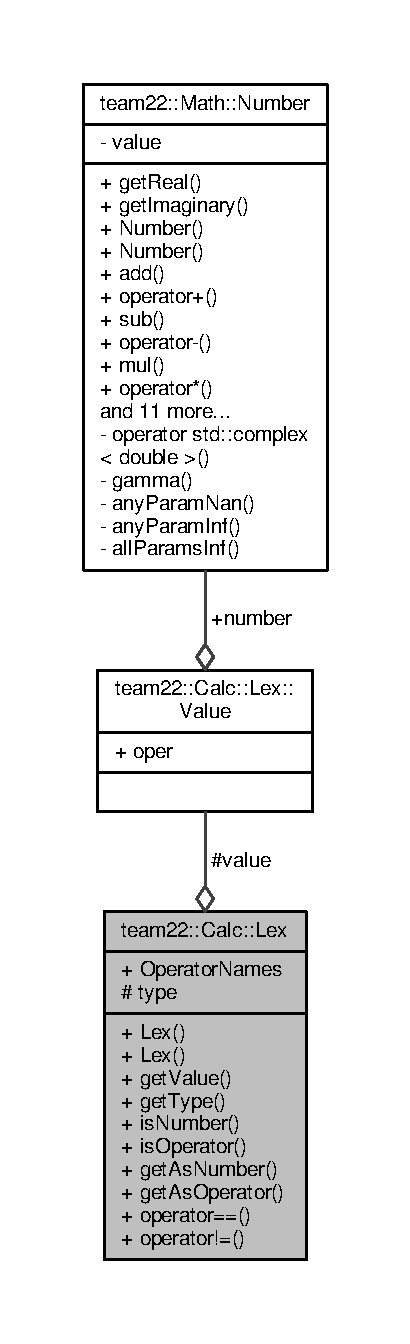
\includegraphics[height=550pt]{classteam22_1_1_calc_1_1_lex__coll__graph}
\end{center}
\end{figure}
\subsection*{Classes}
\begin{DoxyCompactItemize}
\item 
union \hyperlink{unionteam22_1_1_calc_1_1_lex_1_1_value}{Value}
\begin{DoxyCompactList}\small\item\em reprezentace hodnoty lexému \end{DoxyCompactList}\end{DoxyCompactItemize}
\subsection*{Public Types}
\begin{DoxyCompactItemize}
\item 
enum \hyperlink{classteam22_1_1_calc_1_1_lex_a295984577c98a23ddd20ee36d33145a2}{Types} \{ \hyperlink{classteam22_1_1_calc_1_1_lex_a295984577c98a23ddd20ee36d33145a2aa5609722e27933f9074b148e98c70a3b}{O\+P\+E\+R\+A\+T\+OR}, 
\hyperlink{classteam22_1_1_calc_1_1_lex_a295984577c98a23ddd20ee36d33145a2a016603184e8463620cf841dec9b33783}{N\+U\+M\+B\+ER}
 \}\begin{DoxyCompactList}\small\item\em Typy lexémů \end{DoxyCompactList}
\item 
enum \hyperlink{classteam22_1_1_calc_1_1_lex_a61d29fc4878a3b36d2de2f13c56ed932}{Operator} \{ \newline
\hyperlink{classteam22_1_1_calc_1_1_lex_a61d29fc4878a3b36d2de2f13c56ed932a8ea23c5d5cafb66151f94ce0fc7e3677}{A\+DD}, 
\hyperlink{classteam22_1_1_calc_1_1_lex_a61d29fc4878a3b36d2de2f13c56ed932a8fef3694ea5e14ff416907e90fb736c4}{S\+UB}, 
\hyperlink{classteam22_1_1_calc_1_1_lex_a61d29fc4878a3b36d2de2f13c56ed932adb91fbbc380e598b3d09bc424f799516}{D\+IV}, 
\hyperlink{classteam22_1_1_calc_1_1_lex_a61d29fc4878a3b36d2de2f13c56ed932a61a3bc185249f37b2a196b55f3b5a427}{M\+UL}, 
\newline
\hyperlink{classteam22_1_1_calc_1_1_lex_a61d29fc4878a3b36d2de2f13c56ed932ab68440fd94bc855e96432f0734dd6388}{E\+XP}, 
\hyperlink{classteam22_1_1_calc_1_1_lex_a61d29fc4878a3b36d2de2f13c56ed932ad9dc68a37981eff61741cbc660839f6f}{R\+O\+OT}, 
\hyperlink{classteam22_1_1_calc_1_1_lex_a61d29fc4878a3b36d2de2f13c56ed932a88420075287a73244fcaa4f2f851fc65}{F\+A\+C\+T\+O\+R\+I\+AL}, 
\hyperlink{classteam22_1_1_calc_1_1_lex_a61d29fc4878a3b36d2de2f13c56ed932a70d91e1bc184de6388bd44d6fd83e0da}{M\+OD}, 
\newline
\hyperlink{classteam22_1_1_calc_1_1_lex_a61d29fc4878a3b36d2de2f13c56ed932af8b2b375f8262ba1269fe245d7f19853}{N\+EG}, 
\hyperlink{classteam22_1_1_calc_1_1_lex_a61d29fc4878a3b36d2de2f13c56ed932a3c1443c79523cadf6582f238c04a015f}{E\+V\+AL}, 
\hyperlink{classteam22_1_1_calc_1_1_lex_a61d29fc4878a3b36d2de2f13c56ed932a4281d7ef6ac8dbf79c87603ca20c351c}{C\+L\+E\+AR}, 
\hyperlink{classteam22_1_1_calc_1_1_lex_a61d29fc4878a3b36d2de2f13c56ed932ac62fe9cff8a15f20fb1416612309ae80}{BS}
 \}\begin{DoxyCompactList}\small\item\em Jednotlivé operace. \end{DoxyCompactList}
\end{DoxyCompactItemize}
\subsection*{Public Member Functions}
\begin{DoxyCompactItemize}
\item 
\hyperlink{classteam22_1_1_calc_1_1_lex_a12b6acfadebf09ce47319315f8a2e684}{Lex} (\hyperlink{classteam22_1_1_calc_1_1_lex_a61d29fc4878a3b36d2de2f13c56ed932}{Operator} oper)
\begin{DoxyCompactList}\small\item\em Konstrukce lexému typu operátor. \end{DoxyCompactList}\item 
\hyperlink{classteam22_1_1_calc_1_1_lex_a95deefe4c4e987fef602fbd621bac095}{Lex} (\hyperlink{classteam22_1_1_math_1_1_number}{Math\+::\+Number} number)
\begin{DoxyCompactList}\small\item\em Konstrukce lexému typu číslo. \end{DoxyCompactList}\item 
const \hyperlink{unionteam22_1_1_calc_1_1_lex_1_1_value}{Value} \& \hyperlink{classteam22_1_1_calc_1_1_lex_a8a68cd13a68d32d50d3b014ca4478fab}{get\+Value} () const
\begin{DoxyCompactList}\small\item\em vrací hodnotu lexému \end{DoxyCompactList}\item 
\hyperlink{classteam22_1_1_calc_1_1_lex_a295984577c98a23ddd20ee36d33145a2}{Types} \hyperlink{classteam22_1_1_calc_1_1_lex_ae82ccde78beed14c45df1e747ed21bcb}{get\+Type} () const
\begin{DoxyCompactList}\small\item\em vrací typ lexému \end{DoxyCompactList}\item 
bool \hyperlink{classteam22_1_1_calc_1_1_lex_a21f9fe1956185bfb6d80d094846a44f1}{is\+Number} () const
\begin{DoxyCompactList}\small\item\em Testuje zda je lexém číslo. \end{DoxyCompactList}\item 
bool \hyperlink{classteam22_1_1_calc_1_1_lex_a965eff3f3264440279ea9a1f1d3a3cfe}{is\+Operator} () const
\begin{DoxyCompactList}\small\item\em Testuje zda je lexém operátor. \end{DoxyCompactList}\item 
\hyperlink{classteam22_1_1_math_1_1_number}{Math\+::\+Number} \hyperlink{classteam22_1_1_calc_1_1_lex_a794e75373451a906a2cfc60e5d6b1996}{get\+As\+Number} () const
\item 
\hyperlink{classteam22_1_1_calc_1_1_lex_a61d29fc4878a3b36d2de2f13c56ed932}{Operator} \hyperlink{classteam22_1_1_calc_1_1_lex_afdeee7e9b13fcb9826d4d8fd7d5f141f}{get\+As\+Operator} () const
\item 
bool \hyperlink{classteam22_1_1_calc_1_1_lex_a55858e2719cb121fccff59eed42dd692}{operator==} (const \hyperlink{classteam22_1_1_calc_1_1_lex}{Lex} \&rhs) const
\item 
bool \hyperlink{classteam22_1_1_calc_1_1_lex_a25b4f3b98b68c4d967eb3695efc78667}{operator!=} (const \hyperlink{classteam22_1_1_calc_1_1_lex}{Lex} \&rhs) const
\end{DoxyCompactItemize}
\subsection*{Public Attributes}
\begin{DoxyCompactItemize}
\item 
const char $\ast$ \hyperlink{classteam22_1_1_calc_1_1_lex_a9d280854466641dfb02159cc4afeec1f}{Operator\+Names} \mbox{[}12\mbox{]}
\begin{DoxyCompactList}\small\item\em A\+DD,. \end{DoxyCompactList}\end{DoxyCompactItemize}
\subsection*{Protected Attributes}
\begin{DoxyCompactItemize}
\item 
\hyperlink{unionteam22_1_1_calc_1_1_lex_1_1_value}{Value} \hyperlink{classteam22_1_1_calc_1_1_lex_a8a78a736b719931cada0905ac13fedc8}{value}
\item 
\hyperlink{classteam22_1_1_calc_1_1_lex_a295984577c98a23ddd20ee36d33145a2}{Types} \hyperlink{classteam22_1_1_calc_1_1_lex_a733fda9ebfa5ed6f588457d0870e81bc}{type}
\end{DoxyCompactItemize}
\subsection*{Friends}
\begin{DoxyCompactItemize}
\item 
std\+::ostream \& \hyperlink{classteam22_1_1_calc_1_1_lex_aca03505bafd6049109d56fd123d2dae6}{operator$<$$<$} (std\+::ostream \&os, const \hyperlink{classteam22_1_1_calc_1_1_lex}{Lex} \&lex)
\item 
std\+::stringstream \& \hyperlink{classteam22_1_1_calc_1_1_lex_a75f9b47ca9b4289a569608f62336b3dd}{operator$<$$<$} (std\+::stringstream \&os, const \hyperlink{classteam22_1_1_calc_1_1_lex}{Lex} \&lex)
\end{DoxyCompactItemize}


\subsection{Detailed Description}
Reprezentace lexému kalkulačky tedy čísla nebo operace. 

Definition at line 18 of file Lex.\+h.



\subsection{Member Enumeration Documentation}
\mbox{\Hypertarget{classteam22_1_1_calc_1_1_lex_a61d29fc4878a3b36d2de2f13c56ed932}\label{classteam22_1_1_calc_1_1_lex_a61d29fc4878a3b36d2de2f13c56ed932}} 
\index{team22\+::\+Calc\+::\+Lex@{team22\+::\+Calc\+::\+Lex}!Operator@{Operator}}
\index{Operator@{Operator}!team22\+::\+Calc\+::\+Lex@{team22\+::\+Calc\+::\+Lex}}
\subsubsection{\texorpdfstring{Operator}{Operator}}
{\footnotesize\ttfamily enum \hyperlink{classteam22_1_1_calc_1_1_lex_a61d29fc4878a3b36d2de2f13c56ed932}{team22\+::\+Calc\+::\+Lex\+::\+Operator}}



Jednotlivé operace. 

\begin{DoxyEnumFields}{Enumerator}
\raisebox{\heightof{T}}[0pt][0pt]{\index{A\+DD@{A\+DD}!team22\+::\+Calc\+::\+Lex@{team22\+::\+Calc\+::\+Lex}}\index{team22\+::\+Calc\+::\+Lex@{team22\+::\+Calc\+::\+Lex}!A\+DD@{A\+DD}}}\mbox{\Hypertarget{classteam22_1_1_calc_1_1_lex_a61d29fc4878a3b36d2de2f13c56ed932a8ea23c5d5cafb66151f94ce0fc7e3677}\label{classteam22_1_1_calc_1_1_lex_a61d29fc4878a3b36d2de2f13c56ed932a8ea23c5d5cafb66151f94ce0fc7e3677}} 
A\+DD&\\
\hline

\raisebox{\heightof{T}}[0pt][0pt]{\index{S\+UB@{S\+UB}!team22\+::\+Calc\+::\+Lex@{team22\+::\+Calc\+::\+Lex}}\index{team22\+::\+Calc\+::\+Lex@{team22\+::\+Calc\+::\+Lex}!S\+UB@{S\+UB}}}\mbox{\Hypertarget{classteam22_1_1_calc_1_1_lex_a61d29fc4878a3b36d2de2f13c56ed932a8fef3694ea5e14ff416907e90fb736c4}\label{classteam22_1_1_calc_1_1_lex_a61d29fc4878a3b36d2de2f13c56ed932a8fef3694ea5e14ff416907e90fb736c4}} 
S\+UB&\\
\hline

\raisebox{\heightof{T}}[0pt][0pt]{\index{D\+IV@{D\+IV}!team22\+::\+Calc\+::\+Lex@{team22\+::\+Calc\+::\+Lex}}\index{team22\+::\+Calc\+::\+Lex@{team22\+::\+Calc\+::\+Lex}!D\+IV@{D\+IV}}}\mbox{\Hypertarget{classteam22_1_1_calc_1_1_lex_a61d29fc4878a3b36d2de2f13c56ed932adb91fbbc380e598b3d09bc424f799516}\label{classteam22_1_1_calc_1_1_lex_a61d29fc4878a3b36d2de2f13c56ed932adb91fbbc380e598b3d09bc424f799516}} 
D\+IV&\\
\hline

\raisebox{\heightof{T}}[0pt][0pt]{\index{M\+UL@{M\+UL}!team22\+::\+Calc\+::\+Lex@{team22\+::\+Calc\+::\+Lex}}\index{team22\+::\+Calc\+::\+Lex@{team22\+::\+Calc\+::\+Lex}!M\+UL@{M\+UL}}}\mbox{\Hypertarget{classteam22_1_1_calc_1_1_lex_a61d29fc4878a3b36d2de2f13c56ed932a61a3bc185249f37b2a196b55f3b5a427}\label{classteam22_1_1_calc_1_1_lex_a61d29fc4878a3b36d2de2f13c56ed932a61a3bc185249f37b2a196b55f3b5a427}} 
M\+UL&\\
\hline

\raisebox{\heightof{T}}[0pt][0pt]{\index{E\+XP@{E\+XP}!team22\+::\+Calc\+::\+Lex@{team22\+::\+Calc\+::\+Lex}}\index{team22\+::\+Calc\+::\+Lex@{team22\+::\+Calc\+::\+Lex}!E\+XP@{E\+XP}}}\mbox{\Hypertarget{classteam22_1_1_calc_1_1_lex_a61d29fc4878a3b36d2de2f13c56ed932ab68440fd94bc855e96432f0734dd6388}\label{classteam22_1_1_calc_1_1_lex_a61d29fc4878a3b36d2de2f13c56ed932ab68440fd94bc855e96432f0734dd6388}} 
E\+XP&\\
\hline

\raisebox{\heightof{T}}[0pt][0pt]{\index{R\+O\+OT@{R\+O\+OT}!team22\+::\+Calc\+::\+Lex@{team22\+::\+Calc\+::\+Lex}}\index{team22\+::\+Calc\+::\+Lex@{team22\+::\+Calc\+::\+Lex}!R\+O\+OT@{R\+O\+OT}}}\mbox{\Hypertarget{classteam22_1_1_calc_1_1_lex_a61d29fc4878a3b36d2de2f13c56ed932ad9dc68a37981eff61741cbc660839f6f}\label{classteam22_1_1_calc_1_1_lex_a61d29fc4878a3b36d2de2f13c56ed932ad9dc68a37981eff61741cbc660839f6f}} 
R\+O\+OT&\\
\hline

\raisebox{\heightof{T}}[0pt][0pt]{\index{F\+A\+C\+T\+O\+R\+I\+AL@{F\+A\+C\+T\+O\+R\+I\+AL}!team22\+::\+Calc\+::\+Lex@{team22\+::\+Calc\+::\+Lex}}\index{team22\+::\+Calc\+::\+Lex@{team22\+::\+Calc\+::\+Lex}!F\+A\+C\+T\+O\+R\+I\+AL@{F\+A\+C\+T\+O\+R\+I\+AL}}}\mbox{\Hypertarget{classteam22_1_1_calc_1_1_lex_a61d29fc4878a3b36d2de2f13c56ed932a88420075287a73244fcaa4f2f851fc65}\label{classteam22_1_1_calc_1_1_lex_a61d29fc4878a3b36d2de2f13c56ed932a88420075287a73244fcaa4f2f851fc65}} 
F\+A\+C\+T\+O\+R\+I\+AL&\\
\hline

\raisebox{\heightof{T}}[0pt][0pt]{\index{M\+OD@{M\+OD}!team22\+::\+Calc\+::\+Lex@{team22\+::\+Calc\+::\+Lex}}\index{team22\+::\+Calc\+::\+Lex@{team22\+::\+Calc\+::\+Lex}!M\+OD@{M\+OD}}}\mbox{\Hypertarget{classteam22_1_1_calc_1_1_lex_a61d29fc4878a3b36d2de2f13c56ed932a70d91e1bc184de6388bd44d6fd83e0da}\label{classteam22_1_1_calc_1_1_lex_a61d29fc4878a3b36d2de2f13c56ed932a70d91e1bc184de6388bd44d6fd83e0da}} 
M\+OD&\\
\hline

\raisebox{\heightof{T}}[0pt][0pt]{\index{N\+EG@{N\+EG}!team22\+::\+Calc\+::\+Lex@{team22\+::\+Calc\+::\+Lex}}\index{team22\+::\+Calc\+::\+Lex@{team22\+::\+Calc\+::\+Lex}!N\+EG@{N\+EG}}}\mbox{\Hypertarget{classteam22_1_1_calc_1_1_lex_a61d29fc4878a3b36d2de2f13c56ed932af8b2b375f8262ba1269fe245d7f19853}\label{classteam22_1_1_calc_1_1_lex_a61d29fc4878a3b36d2de2f13c56ed932af8b2b375f8262ba1269fe245d7f19853}} 
N\+EG&\\
\hline

\raisebox{\heightof{T}}[0pt][0pt]{\index{E\+V\+AL@{E\+V\+AL}!team22\+::\+Calc\+::\+Lex@{team22\+::\+Calc\+::\+Lex}}\index{team22\+::\+Calc\+::\+Lex@{team22\+::\+Calc\+::\+Lex}!E\+V\+AL@{E\+V\+AL}}}\mbox{\Hypertarget{classteam22_1_1_calc_1_1_lex_a61d29fc4878a3b36d2de2f13c56ed932a3c1443c79523cadf6582f238c04a015f}\label{classteam22_1_1_calc_1_1_lex_a61d29fc4878a3b36d2de2f13c56ed932a3c1443c79523cadf6582f238c04a015f}} 
E\+V\+AL&\\
\hline

\raisebox{\heightof{T}}[0pt][0pt]{\index{C\+L\+E\+AR@{C\+L\+E\+AR}!team22\+::\+Calc\+::\+Lex@{team22\+::\+Calc\+::\+Lex}}\index{team22\+::\+Calc\+::\+Lex@{team22\+::\+Calc\+::\+Lex}!C\+L\+E\+AR@{C\+L\+E\+AR}}}\mbox{\Hypertarget{classteam22_1_1_calc_1_1_lex_a61d29fc4878a3b36d2de2f13c56ed932a4281d7ef6ac8dbf79c87603ca20c351c}\label{classteam22_1_1_calc_1_1_lex_a61d29fc4878a3b36d2de2f13c56ed932a4281d7ef6ac8dbf79c87603ca20c351c}} 
C\+L\+E\+AR&\\
\hline

\raisebox{\heightof{T}}[0pt][0pt]{\index{BS@{BS}!team22\+::\+Calc\+::\+Lex@{team22\+::\+Calc\+::\+Lex}}\index{team22\+::\+Calc\+::\+Lex@{team22\+::\+Calc\+::\+Lex}!BS@{BS}}}\mbox{\Hypertarget{classteam22_1_1_calc_1_1_lex_a61d29fc4878a3b36d2de2f13c56ed932ac62fe9cff8a15f20fb1416612309ae80}\label{classteam22_1_1_calc_1_1_lex_a61d29fc4878a3b36d2de2f13c56ed932ac62fe9cff8a15f20fb1416612309ae80}} 
BS&\\
\hline

\end{DoxyEnumFields}


Definition at line 33 of file Lex.\+h.

\mbox{\Hypertarget{classteam22_1_1_calc_1_1_lex_a295984577c98a23ddd20ee36d33145a2}\label{classteam22_1_1_calc_1_1_lex_a295984577c98a23ddd20ee36d33145a2}} 
\index{team22\+::\+Calc\+::\+Lex@{team22\+::\+Calc\+::\+Lex}!Types@{Types}}
\index{Types@{Types}!team22\+::\+Calc\+::\+Lex@{team22\+::\+Calc\+::\+Lex}}
\subsubsection{\texorpdfstring{Types}{Types}}
{\footnotesize\ttfamily enum \hyperlink{classteam22_1_1_calc_1_1_lex_a295984577c98a23ddd20ee36d33145a2}{team22\+::\+Calc\+::\+Lex\+::\+Types}}



Typy lexémů 

\begin{DoxyEnumFields}{Enumerator}
\raisebox{\heightof{T}}[0pt][0pt]{\index{O\+P\+E\+R\+A\+T\+OR@{O\+P\+E\+R\+A\+T\+OR}!team22\+::\+Calc\+::\+Lex@{team22\+::\+Calc\+::\+Lex}}\index{team22\+::\+Calc\+::\+Lex@{team22\+::\+Calc\+::\+Lex}!O\+P\+E\+R\+A\+T\+OR@{O\+P\+E\+R\+A\+T\+OR}}}\mbox{\Hypertarget{classteam22_1_1_calc_1_1_lex_a295984577c98a23ddd20ee36d33145a2aa5609722e27933f9074b148e98c70a3b}\label{classteam22_1_1_calc_1_1_lex_a295984577c98a23ddd20ee36d33145a2aa5609722e27933f9074b148e98c70a3b}} 
O\+P\+E\+R\+A\+T\+OR&\\
\hline

\raisebox{\heightof{T}}[0pt][0pt]{\index{N\+U\+M\+B\+ER@{N\+U\+M\+B\+ER}!team22\+::\+Calc\+::\+Lex@{team22\+::\+Calc\+::\+Lex}}\index{team22\+::\+Calc\+::\+Lex@{team22\+::\+Calc\+::\+Lex}!N\+U\+M\+B\+ER@{N\+U\+M\+B\+ER}}}\mbox{\Hypertarget{classteam22_1_1_calc_1_1_lex_a295984577c98a23ddd20ee36d33145a2a016603184e8463620cf841dec9b33783}\label{classteam22_1_1_calc_1_1_lex_a295984577c98a23ddd20ee36d33145a2a016603184e8463620cf841dec9b33783}} 
N\+U\+M\+B\+ER&\\
\hline

\end{DoxyEnumFields}


Definition at line 24 of file Lex.\+h.



\subsection{Constructor \& Destructor Documentation}
\mbox{\Hypertarget{classteam22_1_1_calc_1_1_lex_a12b6acfadebf09ce47319315f8a2e684}\label{classteam22_1_1_calc_1_1_lex_a12b6acfadebf09ce47319315f8a2e684}} 
\index{team22\+::\+Calc\+::\+Lex@{team22\+::\+Calc\+::\+Lex}!Lex@{Lex}}
\index{Lex@{Lex}!team22\+::\+Calc\+::\+Lex@{team22\+::\+Calc\+::\+Lex}}
\subsubsection{\texorpdfstring{Lex()}{Lex()}\hspace{0.1cm}{\footnotesize\ttfamily [1/2]}}
{\footnotesize\ttfamily team22\+::\+Calc\+::\+Lex\+::\+Lex (\begin{DoxyParamCaption}\item[{\hyperlink{classteam22_1_1_calc_1_1_lex_a61d29fc4878a3b36d2de2f13c56ed932}{Operator}}]{oper }\end{DoxyParamCaption})}



Konstrukce lexému typu operátor. 


\begin{DoxyParams}{Parameters}
{\em oper} & \\
\hline
\end{DoxyParams}


Definition at line 30 of file Lex.\+cpp.



References team22\+::\+Calc\+::\+Lex\+::\+Value\+::oper, and value.

\mbox{\Hypertarget{classteam22_1_1_calc_1_1_lex_a95deefe4c4e987fef602fbd621bac095}\label{classteam22_1_1_calc_1_1_lex_a95deefe4c4e987fef602fbd621bac095}} 
\index{team22\+::\+Calc\+::\+Lex@{team22\+::\+Calc\+::\+Lex}!Lex@{Lex}}
\index{Lex@{Lex}!team22\+::\+Calc\+::\+Lex@{team22\+::\+Calc\+::\+Lex}}
\subsubsection{\texorpdfstring{Lex()}{Lex()}\hspace{0.1cm}{\footnotesize\ttfamily [2/2]}}
{\footnotesize\ttfamily team22\+::\+Calc\+::\+Lex\+::\+Lex (\begin{DoxyParamCaption}\item[{\hyperlink{classteam22_1_1_math_1_1_number}{Math\+::\+Number}}]{number }\end{DoxyParamCaption})}



Konstrukce lexému typu číslo. 


\begin{DoxyParams}{Parameters}
{\em number} & \\
\hline
\end{DoxyParams}


Definition at line 36 of file Lex.\+cpp.



References team22\+::\+Calc\+::\+Lex\+::\+Value\+::number, and value.



\subsection{Member Function Documentation}
\mbox{\Hypertarget{classteam22_1_1_calc_1_1_lex_a794e75373451a906a2cfc60e5d6b1996}\label{classteam22_1_1_calc_1_1_lex_a794e75373451a906a2cfc60e5d6b1996}} 
\index{team22\+::\+Calc\+::\+Lex@{team22\+::\+Calc\+::\+Lex}!get\+As\+Number@{get\+As\+Number}}
\index{get\+As\+Number@{get\+As\+Number}!team22\+::\+Calc\+::\+Lex@{team22\+::\+Calc\+::\+Lex}}
\subsubsection{\texorpdfstring{get\+As\+Number()}{getAsNumber()}}
{\footnotesize\ttfamily \hyperlink{classteam22_1_1_math_1_1_number}{team22\+::\+Math\+::\+Number} team22\+::\+Calc\+::\+Lex\+::get\+As\+Number (\begin{DoxyParamCaption}{ }\end{DoxyParamCaption}) const}


\begin{DoxyExceptions}{Exceptions}
{\em \hyperlink{classteam22_1_1_calc_1_1_lex_exception}{Lex\+Exception}} & tento lexém pokud není číslo \\
\hline
\end{DoxyExceptions}
\begin{DoxyReturn}{Returns}
number 
\end{DoxyReturn}


Definition at line 42 of file Lex.\+cpp.



References is\+Number(), team22\+::\+Calc\+::\+Lex\+::\+Value\+::number, and value.



Referenced by operator!=(), and operator==().

\mbox{\Hypertarget{classteam22_1_1_calc_1_1_lex_afdeee7e9b13fcb9826d4d8fd7d5f141f}\label{classteam22_1_1_calc_1_1_lex_afdeee7e9b13fcb9826d4d8fd7d5f141f}} 
\index{team22\+::\+Calc\+::\+Lex@{team22\+::\+Calc\+::\+Lex}!get\+As\+Operator@{get\+As\+Operator}}
\index{get\+As\+Operator@{get\+As\+Operator}!team22\+::\+Calc\+::\+Lex@{team22\+::\+Calc\+::\+Lex}}
\subsubsection{\texorpdfstring{get\+As\+Operator()}{getAsOperator()}}
{\footnotesize\ttfamily \hyperlink{classteam22_1_1_calc_1_1_lex_a61d29fc4878a3b36d2de2f13c56ed932}{team22\+::\+Calc\+::\+Lex\+::\+Operator} team22\+::\+Calc\+::\+Lex\+::get\+As\+Operator (\begin{DoxyParamCaption}{ }\end{DoxyParamCaption}) const}


\begin{DoxyExceptions}{Exceptions}
{\em \hyperlink{classteam22_1_1_calc_1_1_lex_exception}{Lex\+Exception}} & tento lexém pokud není Operator \\
\hline
\end{DoxyExceptions}
\begin{DoxyReturn}{Returns}
operator 
\end{DoxyReturn}


Definition at line 50 of file Lex.\+cpp.



References is\+Operator(), team22\+::\+Calc\+::\+Lex\+::\+Value\+::oper, and value.



Referenced by operator!=(), operator==(), and team22\+::\+Calc\+::\+Equation\+::send\+Identified\+Lex().

\mbox{\Hypertarget{classteam22_1_1_calc_1_1_lex_ae82ccde78beed14c45df1e747ed21bcb}\label{classteam22_1_1_calc_1_1_lex_ae82ccde78beed14c45df1e747ed21bcb}} 
\index{team22\+::\+Calc\+::\+Lex@{team22\+::\+Calc\+::\+Lex}!get\+Type@{get\+Type}}
\index{get\+Type@{get\+Type}!team22\+::\+Calc\+::\+Lex@{team22\+::\+Calc\+::\+Lex}}
\subsubsection{\texorpdfstring{get\+Type()}{getType()}}
{\footnotesize\ttfamily \hyperlink{classteam22_1_1_calc_1_1_lex_a295984577c98a23ddd20ee36d33145a2}{team22\+::\+Calc\+::\+Lex\+::\+Types} team22\+::\+Calc\+::\+Lex\+::get\+Type (\begin{DoxyParamCaption}{ }\end{DoxyParamCaption}) const}



vrací typ lexému 

\begin{DoxyReturn}{Returns}
type 
\end{DoxyReturn}


Definition at line 15 of file Lex.\+cpp.



References type.

\mbox{\Hypertarget{classteam22_1_1_calc_1_1_lex_a8a68cd13a68d32d50d3b014ca4478fab}\label{classteam22_1_1_calc_1_1_lex_a8a68cd13a68d32d50d3b014ca4478fab}} 
\index{team22\+::\+Calc\+::\+Lex@{team22\+::\+Calc\+::\+Lex}!get\+Value@{get\+Value}}
\index{get\+Value@{get\+Value}!team22\+::\+Calc\+::\+Lex@{team22\+::\+Calc\+::\+Lex}}
\subsubsection{\texorpdfstring{get\+Value()}{getValue()}}
{\footnotesize\ttfamily const \hyperlink{unionteam22_1_1_calc_1_1_lex_1_1_value}{team22\+::\+Calc\+::\+Lex\+::\+Value} \& team22\+::\+Calc\+::\+Lex\+::get\+Value (\begin{DoxyParamCaption}{ }\end{DoxyParamCaption}) const}



vrací hodnotu lexému 



Definition at line 10 of file Lex.\+cpp.



References value.

\mbox{\Hypertarget{classteam22_1_1_calc_1_1_lex_a21f9fe1956185bfb6d80d094846a44f1}\label{classteam22_1_1_calc_1_1_lex_a21f9fe1956185bfb6d80d094846a44f1}} 
\index{team22\+::\+Calc\+::\+Lex@{team22\+::\+Calc\+::\+Lex}!is\+Number@{is\+Number}}
\index{is\+Number@{is\+Number}!team22\+::\+Calc\+::\+Lex@{team22\+::\+Calc\+::\+Lex}}
\subsubsection{\texorpdfstring{is\+Number()}{isNumber()}}
{\footnotesize\ttfamily bool team22\+::\+Calc\+::\+Lex\+::is\+Number (\begin{DoxyParamCaption}{ }\end{DoxyParamCaption}) const}



Testuje zda je lexém číslo. 

\begin{DoxyReturn}{Returns}
true pokud je číslo 
\end{DoxyReturn}


Definition at line 20 of file Lex.\+cpp.



References type.



Referenced by get\+As\+Number(), operator!=(), and operator==().

\mbox{\Hypertarget{classteam22_1_1_calc_1_1_lex_a965eff3f3264440279ea9a1f1d3a3cfe}\label{classteam22_1_1_calc_1_1_lex_a965eff3f3264440279ea9a1f1d3a3cfe}} 
\index{team22\+::\+Calc\+::\+Lex@{team22\+::\+Calc\+::\+Lex}!is\+Operator@{is\+Operator}}
\index{is\+Operator@{is\+Operator}!team22\+::\+Calc\+::\+Lex@{team22\+::\+Calc\+::\+Lex}}
\subsubsection{\texorpdfstring{is\+Operator()}{isOperator()}}
{\footnotesize\ttfamily bool team22\+::\+Calc\+::\+Lex\+::is\+Operator (\begin{DoxyParamCaption}{ }\end{DoxyParamCaption}) const}



Testuje zda je lexém operátor. 

\begin{DoxyReturn}{Returns}
true pokud je operátor 
\end{DoxyReturn}


Definition at line 25 of file Lex.\+cpp.



References type.



Referenced by get\+As\+Operator(), operator==(), and team22\+::\+Calc\+::\+Equation\+::send\+Identified\+Lex().

\mbox{\Hypertarget{classteam22_1_1_calc_1_1_lex_a25b4f3b98b68c4d967eb3695efc78667}\label{classteam22_1_1_calc_1_1_lex_a25b4f3b98b68c4d967eb3695efc78667}} 
\index{team22\+::\+Calc\+::\+Lex@{team22\+::\+Calc\+::\+Lex}!operator"!=@{operator"!=}}
\index{operator"!=@{operator"!=}!team22\+::\+Calc\+::\+Lex@{team22\+::\+Calc\+::\+Lex}}
\subsubsection{\texorpdfstring{operator"!=()}{operator!=()}}
{\footnotesize\ttfamily bool team22\+::\+Calc\+::\+Lex\+::operator!= (\begin{DoxyParamCaption}\item[{const \hyperlink{classteam22_1_1_calc_1_1_lex}{Lex} \&}]{rhs }\end{DoxyParamCaption}) const}



Definition at line 69 of file Lex.\+cpp.



References get\+As\+Number(), get\+As\+Operator(), is\+Number(), and Operator\+Names.

\mbox{\Hypertarget{classteam22_1_1_calc_1_1_lex_a55858e2719cb121fccff59eed42dd692}\label{classteam22_1_1_calc_1_1_lex_a55858e2719cb121fccff59eed42dd692}} 
\index{team22\+::\+Calc\+::\+Lex@{team22\+::\+Calc\+::\+Lex}!operator==@{operator==}}
\index{operator==@{operator==}!team22\+::\+Calc\+::\+Lex@{team22\+::\+Calc\+::\+Lex}}
\subsubsection{\texorpdfstring{operator==()}{operator==()}}
{\footnotesize\ttfamily bool team22\+::\+Calc\+::\+Lex\+::operator== (\begin{DoxyParamCaption}\item[{const \hyperlink{classteam22_1_1_calc_1_1_lex}{Lex} \&}]{rhs }\end{DoxyParamCaption}) const}



Definition at line 59 of file Lex.\+cpp.



References get\+As\+Number(), get\+As\+Operator(), is\+Number(), is\+Operator(), and type.



\subsection{Friends And Related Function Documentation}
\mbox{\Hypertarget{classteam22_1_1_calc_1_1_lex_aca03505bafd6049109d56fd123d2dae6}\label{classteam22_1_1_calc_1_1_lex_aca03505bafd6049109d56fd123d2dae6}} 
\index{team22\+::\+Calc\+::\+Lex@{team22\+::\+Calc\+::\+Lex}!operator$<$$<$@{operator$<$$<$}}
\index{operator$<$$<$@{operator$<$$<$}!team22\+::\+Calc\+::\+Lex@{team22\+::\+Calc\+::\+Lex}}
\subsubsection{\texorpdfstring{operator$<$$<$}{operator<<}\hspace{0.1cm}{\footnotesize\ttfamily [1/2]}}
{\footnotesize\ttfamily std\+::ostream\& operator$<$$<$ (\begin{DoxyParamCaption}\item[{std\+::ostream \&}]{os,  }\item[{const \hyperlink{classteam22_1_1_calc_1_1_lex}{Lex} \&}]{lex }\end{DoxyParamCaption})\hspace{0.3cm}{\ttfamily [friend]}}

\mbox{\Hypertarget{classteam22_1_1_calc_1_1_lex_a75f9b47ca9b4289a569608f62336b3dd}\label{classteam22_1_1_calc_1_1_lex_a75f9b47ca9b4289a569608f62336b3dd}} 
\index{team22\+::\+Calc\+::\+Lex@{team22\+::\+Calc\+::\+Lex}!operator$<$$<$@{operator$<$$<$}}
\index{operator$<$$<$@{operator$<$$<$}!team22\+::\+Calc\+::\+Lex@{team22\+::\+Calc\+::\+Lex}}
\subsubsection{\texorpdfstring{operator$<$$<$}{operator<<}\hspace{0.1cm}{\footnotesize\ttfamily [2/2]}}
{\footnotesize\ttfamily std\+::stringstream\& operator$<$$<$ (\begin{DoxyParamCaption}\item[{std\+::stringstream \&}]{os,  }\item[{const \hyperlink{classteam22_1_1_calc_1_1_lex}{Lex} \&}]{lex }\end{DoxyParamCaption})\hspace{0.3cm}{\ttfamily [friend]}}



\subsection{Member Data Documentation}
\mbox{\Hypertarget{classteam22_1_1_calc_1_1_lex_a9d280854466641dfb02159cc4afeec1f}\label{classteam22_1_1_calc_1_1_lex_a9d280854466641dfb02159cc4afeec1f}} 
\index{team22\+::\+Calc\+::\+Lex@{team22\+::\+Calc\+::\+Lex}!Operator\+Names@{Operator\+Names}}
\index{Operator\+Names@{Operator\+Names}!team22\+::\+Calc\+::\+Lex@{team22\+::\+Calc\+::\+Lex}}
\subsubsection{\texorpdfstring{Operator\+Names}{OperatorNames}}
{\footnotesize\ttfamily const char$\ast$ team22\+::\+Calc\+::\+Lex\+::\+Operator\+Names\mbox{[}12\mbox{]}}

{\bfseries Initial value\+:}
\begin{DoxyCode}
\{
        \textcolor{stringliteral}{"+"},
        \textcolor{stringliteral}{"-"},
        \textcolor{stringliteral}{"/"},
        \textcolor{stringliteral}{"*"},
        \textcolor{stringliteral}{"^"},
        \textcolor{stringliteral}{"√"},
        \textcolor{stringliteral}{"!"},
        \textcolor{stringliteral}{"%"},
        \textcolor{stringliteral}{"*-1"},
        \textcolor{stringliteral}{"="},
        \textcolor{stringliteral}{"CLEAR"},
        \textcolor{stringliteral}{"BS"},
    \}
\end{DoxyCode}


A\+DD,. 

S\+UB, D\+IV, M\+UL, E\+XP, R\+O\+OT, F\+A\+C\+T\+O\+R\+I\+AL, M\+OD, N\+EG, E\+V\+AL, C\+L\+E\+AR, BS 

Definition at line 49 of file Lex.\+h.



Referenced by operator!=().

\mbox{\Hypertarget{classteam22_1_1_calc_1_1_lex_a733fda9ebfa5ed6f588457d0870e81bc}\label{classteam22_1_1_calc_1_1_lex_a733fda9ebfa5ed6f588457d0870e81bc}} 
\index{team22\+::\+Calc\+::\+Lex@{team22\+::\+Calc\+::\+Lex}!type@{type}}
\index{type@{type}!team22\+::\+Calc\+::\+Lex@{team22\+::\+Calc\+::\+Lex}}
\subsubsection{\texorpdfstring{type}{type}}
{\footnotesize\ttfamily \hyperlink{classteam22_1_1_calc_1_1_lex_a295984577c98a23ddd20ee36d33145a2}{Types} team22\+::\+Calc\+::\+Lex\+::type\hspace{0.3cm}{\ttfamily [protected]}}



Definition at line 75 of file Lex.\+h.



Referenced by get\+Type(), is\+Number(), is\+Operator(), and operator==().

\mbox{\Hypertarget{classteam22_1_1_calc_1_1_lex_a8a78a736b719931cada0905ac13fedc8}\label{classteam22_1_1_calc_1_1_lex_a8a78a736b719931cada0905ac13fedc8}} 
\index{team22\+::\+Calc\+::\+Lex@{team22\+::\+Calc\+::\+Lex}!value@{value}}
\index{value@{value}!team22\+::\+Calc\+::\+Lex@{team22\+::\+Calc\+::\+Lex}}
\subsubsection{\texorpdfstring{value}{value}}
{\footnotesize\ttfamily \hyperlink{unionteam22_1_1_calc_1_1_lex_1_1_value}{Value} team22\+::\+Calc\+::\+Lex\+::value\hspace{0.3cm}{\ttfamily [protected]}}



Definition at line 74 of file Lex.\+h.



Referenced by get\+As\+Number(), get\+As\+Operator(), get\+Value(), and Lex().



The documentation for this class was generated from the following files\+:\begin{DoxyCompactItemize}
\item 
src/\hyperlink{_lex_8h}{Lex.\+h}\item 
src/\hyperlink{_lex_8cpp}{Lex.\+cpp}\end{DoxyCompactItemize}

\hypertarget{classteam22_1_1_calc_1_1_lex_exception}{}\section{team22\+:\+:Calc\+:\+:Lex\+Exception Class Reference}
\label{classteam22_1_1_calc_1_1_lex_exception}\index{team22\+::\+Calc\+::\+Lex\+Exception@{team22\+::\+Calc\+::\+Lex\+Exception}}


{\ttfamily \#include $<$Lex\+Exception.\+h$>$}



Inheritance diagram for team22\+:\+:Calc\+:\+:Lex\+Exception\+:
\nopagebreak
\begin{figure}[H]
\begin{center}
\leavevmode
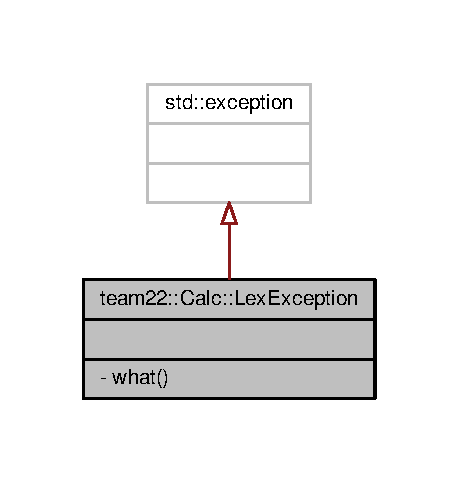
\includegraphics[width=220pt]{classteam22_1_1_calc_1_1_lex_exception__inherit__graph}
\end{center}
\end{figure}


Collaboration diagram for team22\+:\+:Calc\+:\+:Lex\+Exception\+:
\nopagebreak
\begin{figure}[H]
\begin{center}
\leavevmode
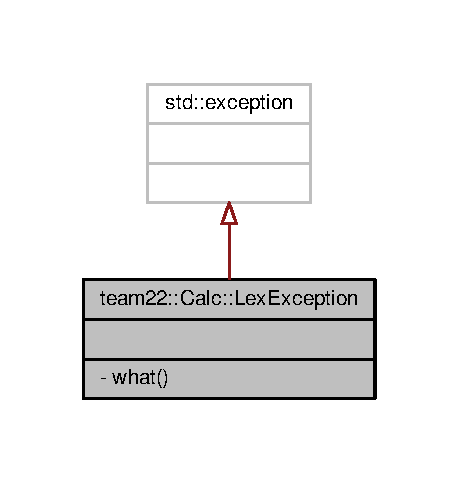
\includegraphics[width=220pt]{classteam22_1_1_calc_1_1_lex_exception__coll__graph}
\end{center}
\end{figure}
\subsection*{Private Member Functions}
\begin{DoxyCompactItemize}
\item 
const char $\ast$ \hyperlink{classteam22_1_1_calc_1_1_lex_exception_afeba1f355eee4aacad8cb7409b1ee3ea}{what} () const noexcept override
\end{DoxyCompactItemize}


\subsection{Detailed Description}
Víjymka pro Lexikální analyzátor 

Definition at line 18 of file Lex\+Exception.\+h.



\subsection{Member Function Documentation}
\mbox{\Hypertarget{classteam22_1_1_calc_1_1_lex_exception_afeba1f355eee4aacad8cb7409b1ee3ea}\label{classteam22_1_1_calc_1_1_lex_exception_afeba1f355eee4aacad8cb7409b1ee3ea}} 
\index{team22\+::\+Calc\+::\+Lex\+Exception@{team22\+::\+Calc\+::\+Lex\+Exception}!what@{what}}
\index{what@{what}!team22\+::\+Calc\+::\+Lex\+Exception@{team22\+::\+Calc\+::\+Lex\+Exception}}
\subsubsection{\texorpdfstring{what()}{what()}}
{\footnotesize\ttfamily const char$\ast$ team22\+::\+Calc\+::\+Lex\+Exception\+::what (\begin{DoxyParamCaption}{ }\end{DoxyParamCaption}) const\hspace{0.3cm}{\ttfamily [inline]}, {\ttfamily [override]}, {\ttfamily [private]}, {\ttfamily [noexcept]}}



Definition at line 23 of file Lex\+Exception.\+h.



The documentation for this class was generated from the following file\+:\begin{DoxyCompactItemize}
\item 
src/\hyperlink{_lex_exception_8h}{Lex\+Exception.\+h}\end{DoxyCompactItemize}

\hypertarget{classteam22_1_1_calc_1_1_lexical_analyzer}{}\section{team22\+:\+:Calc\+:\+:Lexical\+Analyzer Class Reference}
\label{classteam22_1_1_calc_1_1_lexical_analyzer}\index{team22\+::\+Calc\+::\+Lexical\+Analyzer@{team22\+::\+Calc\+::\+Lexical\+Analyzer}}


{\ttfamily \#include $<$Lexical\+Analyzer.\+h$>$}



Collaboration diagram for team22\+:\+:Calc\+:\+:Lexical\+Analyzer\+:
\nopagebreak
\begin{figure}[H]
\begin{center}
\leavevmode
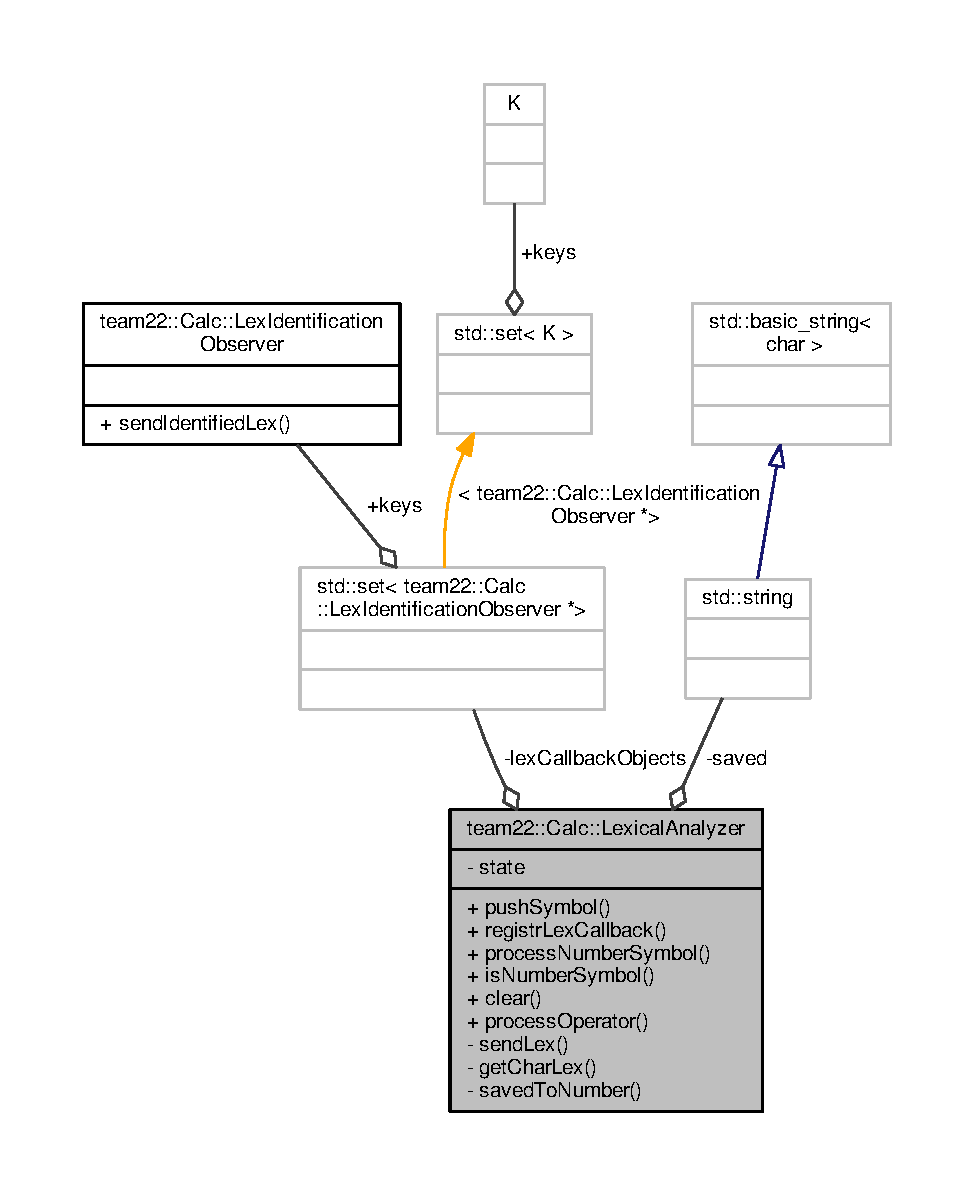
\includegraphics[width=350pt]{classteam22_1_1_calc_1_1_lexical_analyzer__coll__graph}
\end{center}
\end{figure}
\subsection*{Public Member Functions}
\begin{DoxyCompactItemize}
\item 
void \hyperlink{classteam22_1_1_calc_1_1_lexical_analyzer_af56c536f78c680bd635ac1173e65b492}{push\+Symbol} (char symbol)
\item 
void \hyperlink{classteam22_1_1_calc_1_1_lexical_analyzer_ae7fb3f4ce9e6020215352c0c9e2b8245}{registr\+Lex\+Callback} (\hyperlink{classteam22_1_1_calc_1_1_lex_identification_observer}{Lex\+Identification\+Observer} $\ast$lex\+Callback\+Object)
\item 
void \hyperlink{classteam22_1_1_calc_1_1_lexical_analyzer_a18ba04d046da0b11eec66fb2689ddfef}{process\+Number\+Symbol} (char symbol)
\item 
bool \hyperlink{classteam22_1_1_calc_1_1_lexical_analyzer_a922bf14131d064fce52bf126e8d29839}{is\+Number\+Symbol} (char symbol) const
\item 
void \hyperlink{classteam22_1_1_calc_1_1_lexical_analyzer_adf38772b29f998549aa532e8f380b4b2}{clear} ()
\item 
void \hyperlink{classteam22_1_1_calc_1_1_lexical_analyzer_ab84b6b8f52056452cd52b8abdb9a3faa}{process\+Operator} (char symbol)
\end{DoxyCompactItemize}
\subsection*{Private Types}
\begin{DoxyCompactItemize}
\item 
enum \hyperlink{classteam22_1_1_calc_1_1_lexical_analyzer_aef11ba66454715a80d5964c07f6d8cc3}{State} \{ \hyperlink{classteam22_1_1_calc_1_1_lexical_analyzer_aef11ba66454715a80d5964c07f6d8cc3a862f179df5de529676972b3b95c52f86}{Number}, 
\hyperlink{classteam22_1_1_calc_1_1_lexical_analyzer_aef11ba66454715a80d5964c07f6d8cc3ae2510b92e28892c94126aa4273470f78}{Operator}, 
\hyperlink{classteam22_1_1_calc_1_1_lexical_analyzer_aef11ba66454715a80d5964c07f6d8cc3a11976214c837f23fd71b2af8b0de3d5b}{Init}
 \}
\end{DoxyCompactItemize}
\subsection*{Private Member Functions}
\begin{DoxyCompactItemize}
\item 
void \hyperlink{classteam22_1_1_calc_1_1_lexical_analyzer_afd6bb48e5de7f8490addc9b326bfeb49}{send\+Lex} (\hyperlink{classteam22_1_1_calc_1_1_lex}{Lex} lex)
\item 
\hyperlink{classteam22_1_1_calc_1_1_lex}{Lex} \hyperlink{classteam22_1_1_calc_1_1_lexical_analyzer_a451aa3e3ed6f150d5b24fae76cc93cb4}{get\+Char\+Lex} (char \hyperlink{_number_8cpp_a3a6c194a55c239306d07bbf83f5972e9}{c})
\item 
\hyperlink{classteam22_1_1_math_1_1_number}{Math\+::\+Number} \hyperlink{classteam22_1_1_calc_1_1_lexical_analyzer_a689b52c49cd7c9e87dd468987472af83}{saved\+To\+Number} ()
\end{DoxyCompactItemize}
\subsection*{Private Attributes}
\begin{DoxyCompactItemize}
\item 
\hyperlink{classteam22_1_1_calc_1_1_lexical_analyzer_aef11ba66454715a80d5964c07f6d8cc3}{State} \hyperlink{classteam22_1_1_calc_1_1_lexical_analyzer_ad0f4710b09bf91a00d11846a7ef036ab}{state} = \hyperlink{classteam22_1_1_calc_1_1_lexical_analyzer_aef11ba66454715a80d5964c07f6d8cc3a11976214c837f23fd71b2af8b0de3d5b}{Init}
\item 
std\+::set$<$ \hyperlink{classteam22_1_1_calc_1_1_lex_identification_observer}{Lex\+Identification\+Observer} $\ast$ $>$ \hyperlink{classteam22_1_1_calc_1_1_lexical_analyzer_ab8018dc24a6f4e188a901c83bbd9fdb1}{lex\+Callback\+Objects}
\item 
std\+::string \hyperlink{classteam22_1_1_calc_1_1_lexical_analyzer_afd063de2c3d792b5688c863eb5135968}{saved} = \char`\"{}\char`\"{}
\end{DoxyCompactItemize}


\subsection{Detailed Description}
Třída sloužící k lexikální analyze vstupů přebírá znaky pomocí fce \hyperlink{classteam22_1_1_calc_1_1_lexical_analyzer_af56c536f78c680bd635ac1173e65b492}{push\+Symbol()} a ve chvíli identifikace lexému předá tento interpretu a pokud byl registrovaný volá callback kterému tento lexém předá. 

Definition at line 26 of file Lexical\+Analyzer.\+h.



\subsection{Member Enumeration Documentation}
\mbox{\Hypertarget{classteam22_1_1_calc_1_1_lexical_analyzer_aef11ba66454715a80d5964c07f6d8cc3}\label{classteam22_1_1_calc_1_1_lexical_analyzer_aef11ba66454715a80d5964c07f6d8cc3}} 
\index{team22\+::\+Calc\+::\+Lexical\+Analyzer@{team22\+::\+Calc\+::\+Lexical\+Analyzer}!State@{State}}
\index{State@{State}!team22\+::\+Calc\+::\+Lexical\+Analyzer@{team22\+::\+Calc\+::\+Lexical\+Analyzer}}
\subsubsection{\texorpdfstring{State}{State}}
{\footnotesize\ttfamily enum \hyperlink{classteam22_1_1_calc_1_1_lexical_analyzer_aef11ba66454715a80d5964c07f6d8cc3}{team22\+::\+Calc\+::\+Lexical\+Analyzer\+::\+State}\hspace{0.3cm}{\ttfamily [private]}}

\begin{DoxyEnumFields}{Enumerator}
\raisebox{\heightof{T}}[0pt][0pt]{\index{Number@{Number}!team22\+::\+Calc\+::\+Lexical\+Analyzer@{team22\+::\+Calc\+::\+Lexical\+Analyzer}}\index{team22\+::\+Calc\+::\+Lexical\+Analyzer@{team22\+::\+Calc\+::\+Lexical\+Analyzer}!Number@{Number}}}\mbox{\Hypertarget{classteam22_1_1_calc_1_1_lexical_analyzer_aef11ba66454715a80d5964c07f6d8cc3a862f179df5de529676972b3b95c52f86}\label{classteam22_1_1_calc_1_1_lexical_analyzer_aef11ba66454715a80d5964c07f6d8cc3a862f179df5de529676972b3b95c52f86}} 
Number&\\
\hline

\raisebox{\heightof{T}}[0pt][0pt]{\index{Operator@{Operator}!team22\+::\+Calc\+::\+Lexical\+Analyzer@{team22\+::\+Calc\+::\+Lexical\+Analyzer}}\index{team22\+::\+Calc\+::\+Lexical\+Analyzer@{team22\+::\+Calc\+::\+Lexical\+Analyzer}!Operator@{Operator}}}\mbox{\Hypertarget{classteam22_1_1_calc_1_1_lexical_analyzer_aef11ba66454715a80d5964c07f6d8cc3ae2510b92e28892c94126aa4273470f78}\label{classteam22_1_1_calc_1_1_lexical_analyzer_aef11ba66454715a80d5964c07f6d8cc3ae2510b92e28892c94126aa4273470f78}} 
Operator&\\
\hline

\raisebox{\heightof{T}}[0pt][0pt]{\index{Init@{Init}!team22\+::\+Calc\+::\+Lexical\+Analyzer@{team22\+::\+Calc\+::\+Lexical\+Analyzer}}\index{team22\+::\+Calc\+::\+Lexical\+Analyzer@{team22\+::\+Calc\+::\+Lexical\+Analyzer}!Init@{Init}}}\mbox{\Hypertarget{classteam22_1_1_calc_1_1_lexical_analyzer_aef11ba66454715a80d5964c07f6d8cc3a11976214c837f23fd71b2af8b0de3d5b}\label{classteam22_1_1_calc_1_1_lexical_analyzer_aef11ba66454715a80d5964c07f6d8cc3a11976214c837f23fd71b2af8b0de3d5b}} 
Init&\\
\hline

\end{DoxyEnumFields}


Definition at line 28 of file Lexical\+Analyzer.\+h.



\subsection{Member Function Documentation}
\mbox{\Hypertarget{classteam22_1_1_calc_1_1_lexical_analyzer_adf38772b29f998549aa532e8f380b4b2}\label{classteam22_1_1_calc_1_1_lexical_analyzer_adf38772b29f998549aa532e8f380b4b2}} 
\index{team22\+::\+Calc\+::\+Lexical\+Analyzer@{team22\+::\+Calc\+::\+Lexical\+Analyzer}!clear@{clear}}
\index{clear@{clear}!team22\+::\+Calc\+::\+Lexical\+Analyzer@{team22\+::\+Calc\+::\+Lexical\+Analyzer}}
\subsubsection{\texorpdfstring{clear()}{clear()}}
{\footnotesize\ttfamily void team22\+::\+Calc\+::\+Lexical\+Analyzer\+::clear (\begin{DoxyParamCaption}{ }\end{DoxyParamCaption})}

Vyresetuje lexikální analyzátor 

Definition at line 167 of file Lexical\+Analyzer.\+cpp.



References Init, saved, and state.



Referenced by process\+Number\+Symbol(), process\+Operator(), and push\+Symbol().

\mbox{\Hypertarget{classteam22_1_1_calc_1_1_lexical_analyzer_a451aa3e3ed6f150d5b24fae76cc93cb4}\label{classteam22_1_1_calc_1_1_lexical_analyzer_a451aa3e3ed6f150d5b24fae76cc93cb4}} 
\index{team22\+::\+Calc\+::\+Lexical\+Analyzer@{team22\+::\+Calc\+::\+Lexical\+Analyzer}!get\+Char\+Lex@{get\+Char\+Lex}}
\index{get\+Char\+Lex@{get\+Char\+Lex}!team22\+::\+Calc\+::\+Lexical\+Analyzer@{team22\+::\+Calc\+::\+Lexical\+Analyzer}}
\subsubsection{\texorpdfstring{get\+Char\+Lex()}{getCharLex()}}
{\footnotesize\ttfamily \hyperlink{classteam22_1_1_calc_1_1_lex}{Lex} team22\+::\+Calc\+::\+Lexical\+Analyzer\+::get\+Char\+Lex (\begin{DoxyParamCaption}\item[{char}]{c }\end{DoxyParamCaption})\hspace{0.3cm}{\ttfamily [private]}}

Vrací lexém daného znaku 
\begin{DoxyParams}{Parameters}
{\em c} & znak nebo číslice k převodu na lexém \\
\hline
\end{DoxyParams}


Definition at line 19 of file Lexical\+Analyzer.\+cpp.



References team22\+::\+Calc\+::\+Lex\+::\+A\+DD, team22\+::\+Calc\+::\+Lex\+::\+C\+L\+E\+AR, team22\+::\+Calc\+::\+Lex\+::\+D\+IV, team22\+::\+Calc\+::\+Lex\+::\+E\+V\+AL, team22\+::\+Calc\+::\+Lex\+::\+E\+XP, team22\+::\+Calc\+::\+Lex\+::\+F\+A\+C\+T\+O\+R\+I\+AL, team22\+::\+Calc\+::\+Lex\+::\+M\+OD, team22\+::\+Calc\+::\+Lex\+::\+M\+UL, and team22\+::\+Calc\+::\+Lex\+::\+S\+UB.



Referenced by push\+Symbol().

\mbox{\Hypertarget{classteam22_1_1_calc_1_1_lexical_analyzer_a922bf14131d064fce52bf126e8d29839}\label{classteam22_1_1_calc_1_1_lexical_analyzer_a922bf14131d064fce52bf126e8d29839}} 
\index{team22\+::\+Calc\+::\+Lexical\+Analyzer@{team22\+::\+Calc\+::\+Lexical\+Analyzer}!is\+Number\+Symbol@{is\+Number\+Symbol}}
\index{is\+Number\+Symbol@{is\+Number\+Symbol}!team22\+::\+Calc\+::\+Lexical\+Analyzer@{team22\+::\+Calc\+::\+Lexical\+Analyzer}}
\subsubsection{\texorpdfstring{is\+Number\+Symbol()}{isNumberSymbol()}}
{\footnotesize\ttfamily bool team22\+::\+Calc\+::\+Lexical\+Analyzer\+::is\+Number\+Symbol (\begin{DoxyParamCaption}\item[{char}]{symbol }\end{DoxyParamCaption}) const}

Jedná se o symbol tvořící číslo tedy číslice, . nebo i 
\begin{DoxyParams}{Parameters}
{\em symbol} & \\
\hline
\end{DoxyParams}
\begin{DoxyReturn}{Returns}

\end{DoxyReturn}


Definition at line 138 of file Lexical\+Analyzer.\+cpp.



Referenced by push\+Symbol().

\mbox{\Hypertarget{classteam22_1_1_calc_1_1_lexical_analyzer_a18ba04d046da0b11eec66fb2689ddfef}\label{classteam22_1_1_calc_1_1_lexical_analyzer_a18ba04d046da0b11eec66fb2689ddfef}} 
\index{team22\+::\+Calc\+::\+Lexical\+Analyzer@{team22\+::\+Calc\+::\+Lexical\+Analyzer}!process\+Number\+Symbol@{process\+Number\+Symbol}}
\index{process\+Number\+Symbol@{process\+Number\+Symbol}!team22\+::\+Calc\+::\+Lexical\+Analyzer@{team22\+::\+Calc\+::\+Lexical\+Analyzer}}
\subsubsection{\texorpdfstring{process\+Number\+Symbol()}{processNumberSymbol()}}
{\footnotesize\ttfamily void team22\+::\+Calc\+::\+Lexical\+Analyzer\+::process\+Number\+Symbol (\begin{DoxyParamCaption}\item[{char}]{symbol }\end{DoxyParamCaption})}

Zpracuje uložený řetězec saved a vrátí jej jako číslo 
\begin{DoxyParams}{Parameters}
{\em symbol} & \\
\hline
\end{DoxyParams}


Definition at line 148 of file Lexical\+Analyzer.\+cpp.



References clear(), Init, Number, saved, saved\+To\+Number(), send\+Lex(), and state.



Referenced by push\+Symbol().

\mbox{\Hypertarget{classteam22_1_1_calc_1_1_lexical_analyzer_ab84b6b8f52056452cd52b8abdb9a3faa}\label{classteam22_1_1_calc_1_1_lexical_analyzer_ab84b6b8f52056452cd52b8abdb9a3faa}} 
\index{team22\+::\+Calc\+::\+Lexical\+Analyzer@{team22\+::\+Calc\+::\+Lexical\+Analyzer}!process\+Operator@{process\+Operator}}
\index{process\+Operator@{process\+Operator}!team22\+::\+Calc\+::\+Lexical\+Analyzer@{team22\+::\+Calc\+::\+Lexical\+Analyzer}}
\subsubsection{\texorpdfstring{process\+Operator()}{processOperator()}}
{\footnotesize\ttfamily void team22\+::\+Calc\+::\+Lexical\+Analyzer\+::process\+Operator (\begin{DoxyParamCaption}\item[{char}]{symbol }\end{DoxyParamCaption})}

Zpracuje výceznakový operátor 
\begin{DoxyParams}{Parameters}
{\em symbol} & \\
\hline
\end{DoxyParams}


Definition at line 80 of file Lexical\+Analyzer.\+cpp.



References team22\+::\+Calc\+::\+Lex\+::\+BS, clear(), team22\+::\+Calc\+::\+Lex\+::\+N\+EG, Operator, team22\+::\+Calc\+::\+Lex\+::\+R\+O\+OT, saved, send\+Lex(), and state.



Referenced by push\+Symbol().

\mbox{\Hypertarget{classteam22_1_1_calc_1_1_lexical_analyzer_af56c536f78c680bd635ac1173e65b492}\label{classteam22_1_1_calc_1_1_lexical_analyzer_af56c536f78c680bd635ac1173e65b492}} 
\index{team22\+::\+Calc\+::\+Lexical\+Analyzer@{team22\+::\+Calc\+::\+Lexical\+Analyzer}!push\+Symbol@{push\+Symbol}}
\index{push\+Symbol@{push\+Symbol}!team22\+::\+Calc\+::\+Lexical\+Analyzer@{team22\+::\+Calc\+::\+Lexical\+Analyzer}}
\subsubsection{\texorpdfstring{push\+Symbol()}{pushSymbol()}}
{\footnotesize\ttfamily void team22\+::\+Calc\+::\+Lexical\+Analyzer\+::push\+Symbol (\begin{DoxyParamCaption}\item[{char}]{symbol }\end{DoxyParamCaption})}

Předá znak k analýze 
\begin{DoxyParams}{Parameters}
{\em symbol} & symbol abecedy přijímané lexikálním analyzátorem \\
\hline
\end{DoxyParams}

\begin{DoxyExceptions}{Exceptions}
{\em Lexical\+Analyser\+Exception} & \\
\hline
\end{DoxyExceptions}


Definition at line 61 of file Lexical\+Analyzer.\+cpp.



References clear(), get\+Char\+Lex(), is\+Number\+Symbol(), Number, process\+Number\+Symbol(), process\+Operator(), saved\+To\+Number(), send\+Lex(), and state.



Referenced by team22\+::\+Calc\+::\+Equation\+::back\+Space(), and team22\+::\+Calc\+::\+Equation\+::push\+Symbol().

\mbox{\Hypertarget{classteam22_1_1_calc_1_1_lexical_analyzer_ae7fb3f4ce9e6020215352c0c9e2b8245}\label{classteam22_1_1_calc_1_1_lexical_analyzer_ae7fb3f4ce9e6020215352c0c9e2b8245}} 
\index{team22\+::\+Calc\+::\+Lexical\+Analyzer@{team22\+::\+Calc\+::\+Lexical\+Analyzer}!registr\+Lex\+Callback@{registr\+Lex\+Callback}}
\index{registr\+Lex\+Callback@{registr\+Lex\+Callback}!team22\+::\+Calc\+::\+Lexical\+Analyzer@{team22\+::\+Calc\+::\+Lexical\+Analyzer}}
\subsubsection{\texorpdfstring{registr\+Lex\+Callback()}{registrLexCallback()}}
{\footnotesize\ttfamily void team22\+::\+Calc\+::\+Lexical\+Analyzer\+::registr\+Lex\+Callback (\begin{DoxyParamCaption}\item[{\hyperlink{classteam22_1_1_calc_1_1_lex_identification_observer}{Lex\+Identification\+Observer} $\ast$}]{lex\+Callback\+Object }\end{DoxyParamCaption})}

Registruje objekt k odběru rozeznaných lexémů vícenásobná registrace stejné instance odběratele neprovede nic


\begin{DoxyParams}{Parameters}
{\em lex\+Callback\+Object} & objekt na němž \\
\hline
\end{DoxyParams}


Definition at line 143 of file Lexical\+Analyzer.\+cpp.



References lex\+Callback\+Objects.



Referenced by Backend\+Tester\+::\+Backend\+Tester(), team22\+::\+Calc\+::\+Equation\+::\+Equation(), and Lexical\+Analyzer\+Test\+Base\+::\+Lexical\+Analyzer\+Test\+Base().

\mbox{\Hypertarget{classteam22_1_1_calc_1_1_lexical_analyzer_a689b52c49cd7c9e87dd468987472af83}\label{classteam22_1_1_calc_1_1_lexical_analyzer_a689b52c49cd7c9e87dd468987472af83}} 
\index{team22\+::\+Calc\+::\+Lexical\+Analyzer@{team22\+::\+Calc\+::\+Lexical\+Analyzer}!saved\+To\+Number@{saved\+To\+Number}}
\index{saved\+To\+Number@{saved\+To\+Number}!team22\+::\+Calc\+::\+Lexical\+Analyzer@{team22\+::\+Calc\+::\+Lexical\+Analyzer}}
\subsubsection{\texorpdfstring{saved\+To\+Number()}{savedToNumber()}}
{\footnotesize\ttfamily \hyperlink{classteam22_1_1_math_1_1_number}{Math\+::\+Number} team22\+::\+Calc\+::\+Lexical\+Analyzer\+::saved\+To\+Number (\begin{DoxyParamCaption}{ }\end{DoxyParamCaption})\hspace{0.3cm}{\ttfamily [private]}}

Vrací číslo typu double převedené z textového řetězce 
\begin{DoxyParams}{Parameters}
{\em s} & textový řetězec pro převod \\
\hline
\end{DoxyParams}


Definition at line 45 of file Lexical\+Analyzer.\+cpp.



References saved.



Referenced by process\+Number\+Symbol(), and push\+Symbol().

\mbox{\Hypertarget{classteam22_1_1_calc_1_1_lexical_analyzer_afd6bb48e5de7f8490addc9b326bfeb49}\label{classteam22_1_1_calc_1_1_lexical_analyzer_afd6bb48e5de7f8490addc9b326bfeb49}} 
\index{team22\+::\+Calc\+::\+Lexical\+Analyzer@{team22\+::\+Calc\+::\+Lexical\+Analyzer}!send\+Lex@{send\+Lex}}
\index{send\+Lex@{send\+Lex}!team22\+::\+Calc\+::\+Lexical\+Analyzer@{team22\+::\+Calc\+::\+Lexical\+Analyzer}}
\subsubsection{\texorpdfstring{send\+Lex()}{sendLex()}}
{\footnotesize\ttfamily void team22\+::\+Calc\+::\+Lexical\+Analyzer\+::send\+Lex (\begin{DoxyParamCaption}\item[{\hyperlink{classteam22_1_1_calc_1_1_lex}{Lex}}]{lex }\end{DoxyParamCaption})\hspace{0.3cm}{\ttfamily [private]}}

Předá lexém všem registrovaným objektům 
\begin{DoxyParams}{Parameters}
{\em lex} & lexém k předání \\
\hline
\end{DoxyParams}


Definition at line 13 of file Lexical\+Analyzer.\+cpp.



References lex\+Callback\+Objects.



Referenced by process\+Number\+Symbol(), process\+Operator(), and push\+Symbol().



\subsection{Member Data Documentation}
\mbox{\Hypertarget{classteam22_1_1_calc_1_1_lexical_analyzer_ab8018dc24a6f4e188a901c83bbd9fdb1}\label{classteam22_1_1_calc_1_1_lexical_analyzer_ab8018dc24a6f4e188a901c83bbd9fdb1}} 
\index{team22\+::\+Calc\+::\+Lexical\+Analyzer@{team22\+::\+Calc\+::\+Lexical\+Analyzer}!lex\+Callback\+Objects@{lex\+Callback\+Objects}}
\index{lex\+Callback\+Objects@{lex\+Callback\+Objects}!team22\+::\+Calc\+::\+Lexical\+Analyzer@{team22\+::\+Calc\+::\+Lexical\+Analyzer}}
\subsubsection{\texorpdfstring{lex\+Callback\+Objects}{lexCallbackObjects}}
{\footnotesize\ttfamily std\+::set$<$\hyperlink{classteam22_1_1_calc_1_1_lex_identification_observer}{Lex\+Identification\+Observer} $\ast$$>$ team22\+::\+Calc\+::\+Lexical\+Analyzer\+::lex\+Callback\+Objects\hspace{0.3cm}{\ttfamily [private]}}

Množina Objektů na nichž bude volán callback při rozeznání lexemů 

Definition at line 39 of file Lexical\+Analyzer.\+h.



Referenced by registr\+Lex\+Callback(), and send\+Lex().

\mbox{\Hypertarget{classteam22_1_1_calc_1_1_lexical_analyzer_afd063de2c3d792b5688c863eb5135968}\label{classteam22_1_1_calc_1_1_lexical_analyzer_afd063de2c3d792b5688c863eb5135968}} 
\index{team22\+::\+Calc\+::\+Lexical\+Analyzer@{team22\+::\+Calc\+::\+Lexical\+Analyzer}!saved@{saved}}
\index{saved@{saved}!team22\+::\+Calc\+::\+Lexical\+Analyzer@{team22\+::\+Calc\+::\+Lexical\+Analyzer}}
\subsubsection{\texorpdfstring{saved}{saved}}
{\footnotesize\ttfamily std\+::string team22\+::\+Calc\+::\+Lexical\+Analyzer\+::saved = \char`\"{}\char`\"{}\hspace{0.3cm}{\ttfamily [private]}}

Řetězec, který obsahuje znaky, které ještě nebyly rozeznány jako lexém 

Definition at line 44 of file Lexical\+Analyzer.\+h.



Referenced by clear(), process\+Number\+Symbol(), process\+Operator(), and saved\+To\+Number().

\mbox{\Hypertarget{classteam22_1_1_calc_1_1_lexical_analyzer_ad0f4710b09bf91a00d11846a7ef036ab}\label{classteam22_1_1_calc_1_1_lexical_analyzer_ad0f4710b09bf91a00d11846a7ef036ab}} 
\index{team22\+::\+Calc\+::\+Lexical\+Analyzer@{team22\+::\+Calc\+::\+Lexical\+Analyzer}!state@{state}}
\index{state@{state}!team22\+::\+Calc\+::\+Lexical\+Analyzer@{team22\+::\+Calc\+::\+Lexical\+Analyzer}}
\subsubsection{\texorpdfstring{state}{state}}
{\footnotesize\ttfamily \hyperlink{classteam22_1_1_calc_1_1_lexical_analyzer_aef11ba66454715a80d5964c07f6d8cc3}{State} team22\+::\+Calc\+::\+Lexical\+Analyzer\+::state = \hyperlink{classteam22_1_1_calc_1_1_lexical_analyzer_aef11ba66454715a80d5964c07f6d8cc3a11976214c837f23fd71b2af8b0de3d5b}{Init}\hspace{0.3cm}{\ttfamily [private]}}



Definition at line 34 of file Lexical\+Analyzer.\+h.



Referenced by clear(), process\+Number\+Symbol(), process\+Operator(), and push\+Symbol().



The documentation for this class was generated from the following files\+:\begin{DoxyCompactItemize}
\item 
src/\hyperlink{_lexical_analyzer_8h}{Lexical\+Analyzer.\+h}\item 
src/\hyperlink{_lexical_analyzer_8cpp}{Lexical\+Analyzer.\+cpp}\end{DoxyCompactItemize}

\hypertarget{struct_lexical_analyzer_errors_test}{}\section{Lexical\+Analyzer\+Errors\+Test Struct Reference}
\label{struct_lexical_analyzer_errors_test}\index{Lexical\+Analyzer\+Errors\+Test@{Lexical\+Analyzer\+Errors\+Test}}


Inheritance diagram for Lexical\+Analyzer\+Errors\+Test\+:
\nopagebreak
\begin{figure}[H]
\begin{center}
\leavevmode
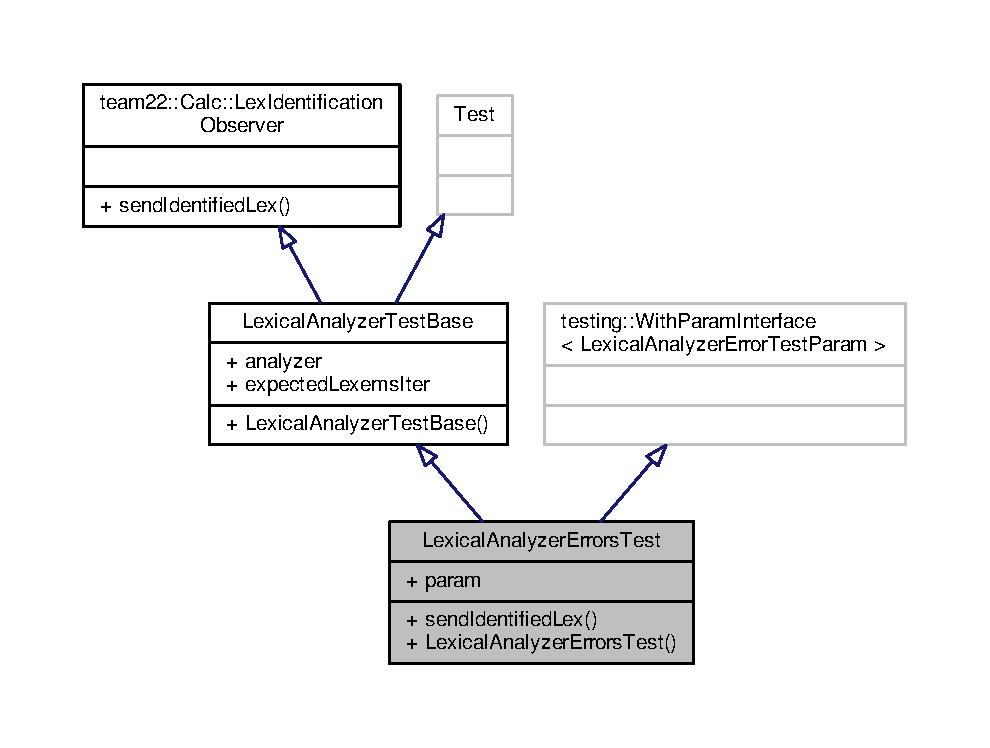
\includegraphics[width=350pt]{struct_lexical_analyzer_errors_test__inherit__graph}
\end{center}
\end{figure}


Collaboration diagram for Lexical\+Analyzer\+Errors\+Test\+:
\nopagebreak
\begin{figure}[H]
\begin{center}
\leavevmode
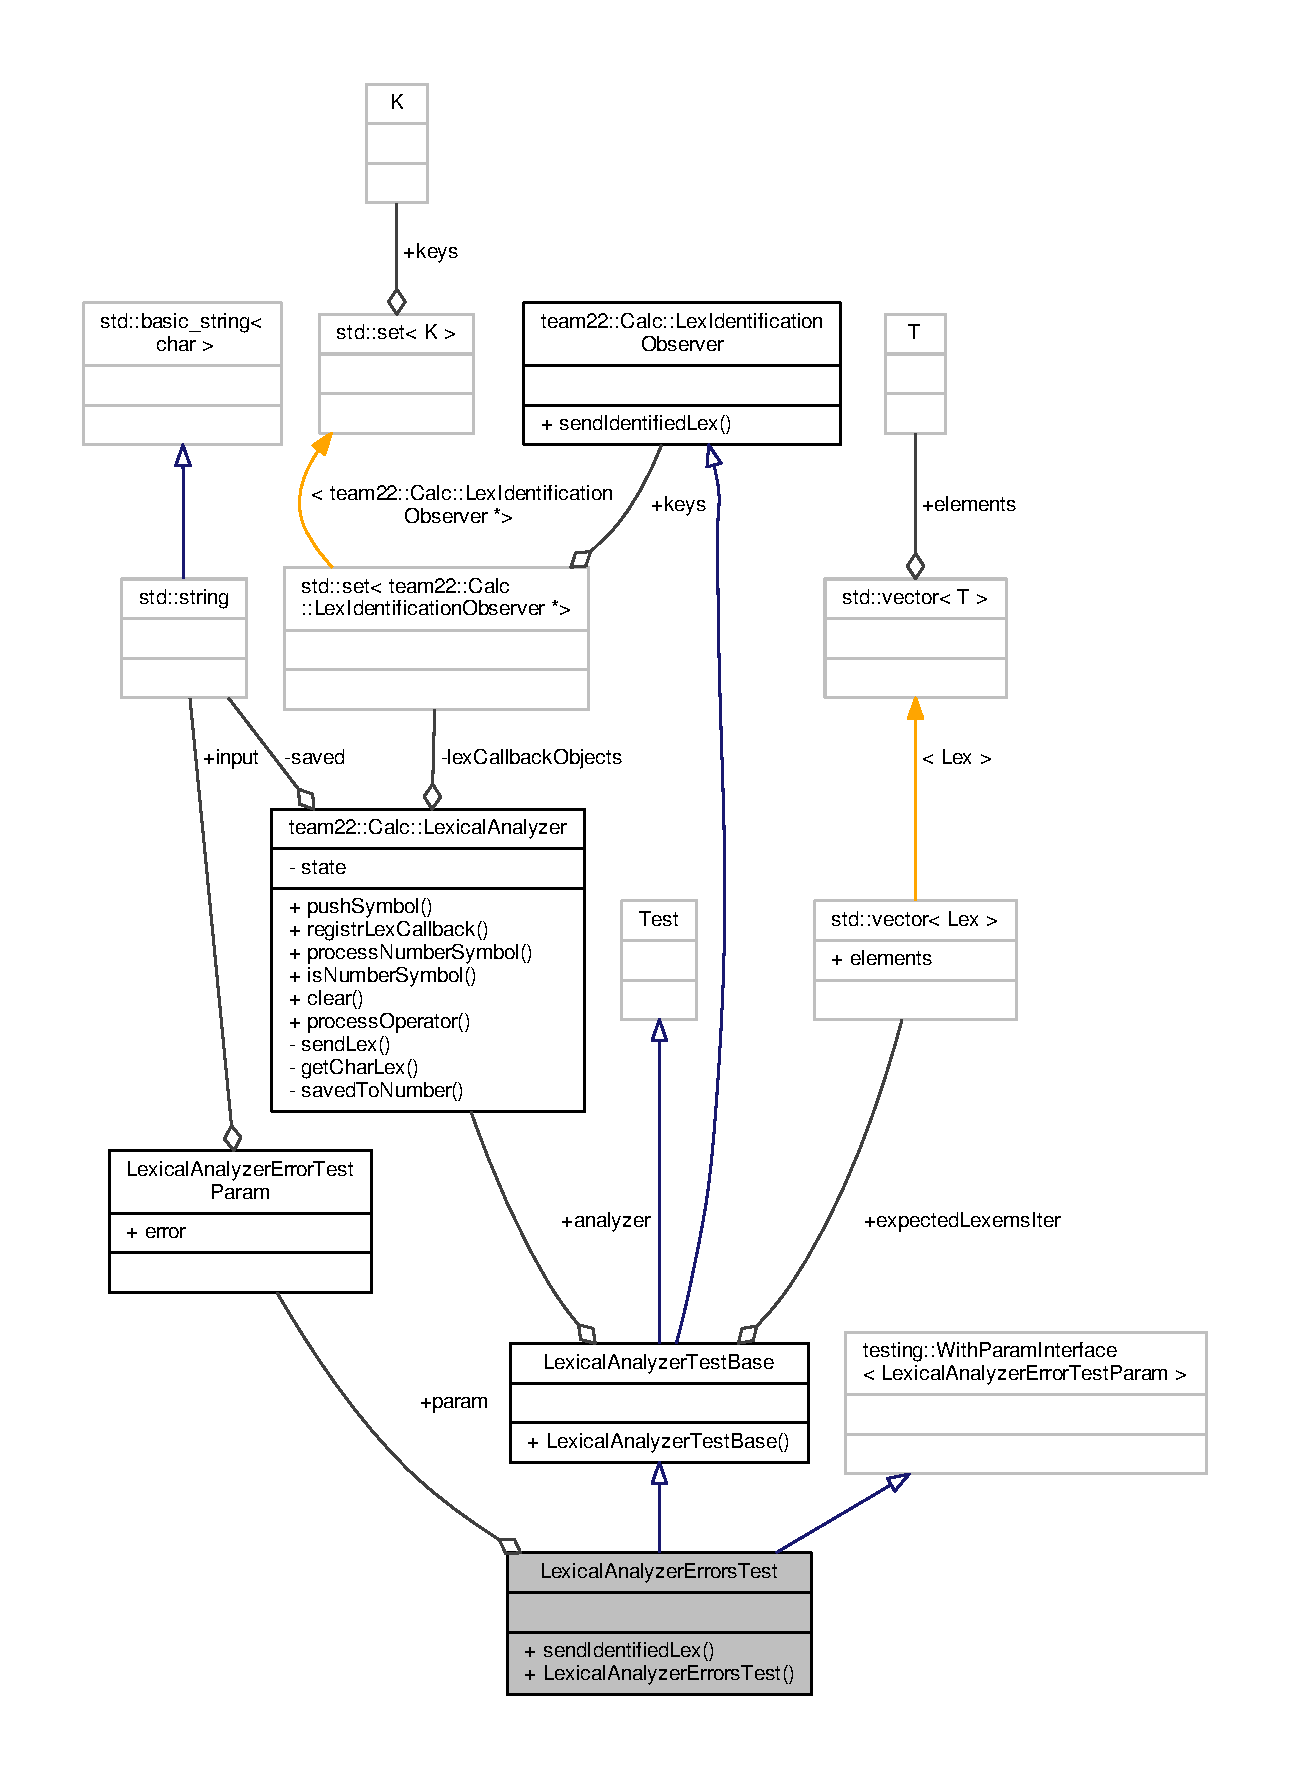
\includegraphics[width=350pt]{struct_lexical_analyzer_errors_test__coll__graph}
\end{center}
\end{figure}
\subsection*{Public Member Functions}
\begin{DoxyCompactItemize}
\item 
void \hyperlink{struct_lexical_analyzer_errors_test_ac943a4238a0eb77957e2027740603c44}{send\+Identified\+Lex} (\hyperlink{classteam22_1_1_calc_1_1_lex}{Lex} lex) override
\item 
\hyperlink{struct_lexical_analyzer_errors_test_ae4fdca5d1de2494ca722d4683e62bc16}{Lexical\+Analyzer\+Errors\+Test} ()
\end{DoxyCompactItemize}
\subsection*{Public Attributes}
\begin{DoxyCompactItemize}
\item 
\hyperlink{struct_lexical_analyzer_error_test_param}{Lexical\+Analyzer\+Error\+Test\+Param} \hyperlink{struct_lexical_analyzer_errors_test_a61a8ef433e2118a8723bfd8f99029126}{param}
\end{DoxyCompactItemize}


\subsection{Detailed Description}


Definition at line 82 of file Lexical\+Analyzer\+Test.\+cpp.



\subsection{Constructor \& Destructor Documentation}
\mbox{\Hypertarget{struct_lexical_analyzer_errors_test_ae4fdca5d1de2494ca722d4683e62bc16}\label{struct_lexical_analyzer_errors_test_ae4fdca5d1de2494ca722d4683e62bc16}} 
\index{Lexical\+Analyzer\+Errors\+Test@{Lexical\+Analyzer\+Errors\+Test}!Lexical\+Analyzer\+Errors\+Test@{Lexical\+Analyzer\+Errors\+Test}}
\index{Lexical\+Analyzer\+Errors\+Test@{Lexical\+Analyzer\+Errors\+Test}!Lexical\+Analyzer\+Errors\+Test@{Lexical\+Analyzer\+Errors\+Test}}
\subsubsection{\texorpdfstring{Lexical\+Analyzer\+Errors\+Test()}{LexicalAnalyzerErrorsTest()}}
{\footnotesize\ttfamily Lexical\+Analyzer\+Errors\+Test\+::\+Lexical\+Analyzer\+Errors\+Test (\begin{DoxyParamCaption}{ }\end{DoxyParamCaption})\hspace{0.3cm}{\ttfamily [inline]}}



Definition at line 89 of file Lexical\+Analyzer\+Test.\+cpp.



References team22\+::\+Calc\+::\+Lex\+::\+A\+DD, team22\+::\+Calc\+::\+Lex\+::\+BS, team22\+::\+Calc\+::\+Lex\+::\+C\+L\+E\+AR, team22\+::\+Calc\+::\+Lex\+::\+D\+IV, team22\+::\+Calc\+::\+Lex\+::\+E\+V\+AL, team22\+::\+Calc\+::\+Lex\+::\+E\+XP, team22\+::\+Calc\+::\+Lex\+::\+F\+A\+C\+T\+O\+R\+I\+AL, I\+N\+S\+T\+A\+N\+T\+I\+A\+T\+E\+\_\+\+T\+E\+S\+T\+\_\+\+C\+A\+S\+E\+\_\+\+P(), team22\+::\+Calc\+::\+Lex\+::\+M\+OD, team22\+::\+Calc\+::\+Lex\+::\+M\+UL, team22\+::\+Calc\+::\+Lex\+::\+N\+EG, team22\+::\+Calc\+::\+Lex\+::\+R\+O\+OT, and team22\+::\+Calc\+::\+Lex\+::\+S\+UB.



\subsection{Member Function Documentation}
\mbox{\Hypertarget{struct_lexical_analyzer_errors_test_ac943a4238a0eb77957e2027740603c44}\label{struct_lexical_analyzer_errors_test_ac943a4238a0eb77957e2027740603c44}} 
\index{Lexical\+Analyzer\+Errors\+Test@{Lexical\+Analyzer\+Errors\+Test}!send\+Identified\+Lex@{send\+Identified\+Lex}}
\index{send\+Identified\+Lex@{send\+Identified\+Lex}!Lexical\+Analyzer\+Errors\+Test@{Lexical\+Analyzer\+Errors\+Test}}
\subsubsection{\texorpdfstring{send\+Identified\+Lex()}{sendIdentifiedLex()}}
{\footnotesize\ttfamily void Lexical\+Analyzer\+Errors\+Test\+::send\+Identified\+Lex (\begin{DoxyParamCaption}\item[{\hyperlink{classteam22_1_1_calc_1_1_lex}{Lex}}]{lex }\end{DoxyParamCaption})\hspace{0.3cm}{\ttfamily [inline]}, {\ttfamily [override]}, {\ttfamily [virtual]}}



Implements \hyperlink{classteam22_1_1_calc_1_1_lex_identification_observer_ac139f75c560625ec6fdb2e34cf0d4884}{team22\+::\+Calc\+::\+Lex\+Identification\+Observer}.



Definition at line 86 of file Lexical\+Analyzer\+Test.\+cpp.



\subsection{Member Data Documentation}
\mbox{\Hypertarget{struct_lexical_analyzer_errors_test_a61a8ef433e2118a8723bfd8f99029126}\label{struct_lexical_analyzer_errors_test_a61a8ef433e2118a8723bfd8f99029126}} 
\index{Lexical\+Analyzer\+Errors\+Test@{Lexical\+Analyzer\+Errors\+Test}!param@{param}}
\index{param@{param}!Lexical\+Analyzer\+Errors\+Test@{Lexical\+Analyzer\+Errors\+Test}}
\subsubsection{\texorpdfstring{param}{param}}
{\footnotesize\ttfamily \hyperlink{struct_lexical_analyzer_error_test_param}{Lexical\+Analyzer\+Error\+Test\+Param} Lexical\+Analyzer\+Errors\+Test\+::param}



Definition at line 84 of file Lexical\+Analyzer\+Test.\+cpp.



The documentation for this struct was generated from the following file\+:\begin{DoxyCompactItemize}
\item 
tests/\hyperlink{_lexical_analyzer_test_8cpp}{Lexical\+Analyzer\+Test.\+cpp}\end{DoxyCompactItemize}

\hypertarget{struct_lexical_analyzer_error_test_param}{}\section{Lexical\+Analyzer\+Error\+Test\+Param Struct Reference}
\label{struct_lexical_analyzer_error_test_param}\index{Lexical\+Analyzer\+Error\+Test\+Param@{Lexical\+Analyzer\+Error\+Test\+Param}}


Collaboration diagram for Lexical\+Analyzer\+Error\+Test\+Param\+:
\nopagebreak
\begin{figure}[H]
\begin{center}
\leavevmode
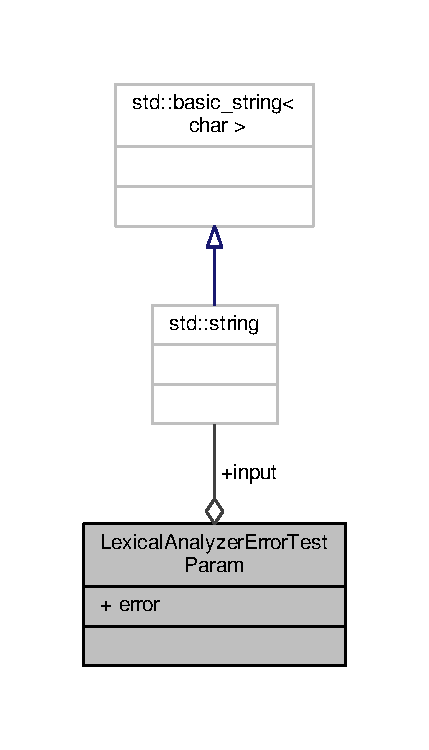
\includegraphics[width=206pt]{struct_lexical_analyzer_error_test_param__coll__graph}
\end{center}
\end{figure}
\subsection*{Public Attributes}
\begin{DoxyCompactItemize}
\item 
string \hyperlink{struct_lexical_analyzer_error_test_param_ab55190d65d3bcaab962dcbe15bd60953}{input}
\item 
char \hyperlink{struct_lexical_analyzer_error_test_param_aab37ca9d0544a4299b23e2c77f9c309c}{error} = \textquotesingle{}0\textquotesingle{}
\end{DoxyCompactItemize}
\subsection*{Friends}
\begin{DoxyCompactItemize}
\item 
std\+::ostream \& \hyperlink{struct_lexical_analyzer_error_test_param_adb9977e1fb31c903604273b3c51be7d6}{operator$<$$<$} (std\+::ostream \&os, const \hyperlink{struct_lexical_analyzer_error_test_param}{Lexical\+Analyzer\+Error\+Test\+Param} \&param)
\end{DoxyCompactItemize}


\subsection{Detailed Description}


Definition at line 38 of file Lexical\+Analyzer\+Test.\+cpp.



\subsection{Friends And Related Function Documentation}
\mbox{\Hypertarget{struct_lexical_analyzer_error_test_param_adb9977e1fb31c903604273b3c51be7d6}\label{struct_lexical_analyzer_error_test_param_adb9977e1fb31c903604273b3c51be7d6}} 
\index{Lexical\+Analyzer\+Error\+Test\+Param@{Lexical\+Analyzer\+Error\+Test\+Param}!operator$<$$<$@{operator$<$$<$}}
\index{operator$<$$<$@{operator$<$$<$}!Lexical\+Analyzer\+Error\+Test\+Param@{Lexical\+Analyzer\+Error\+Test\+Param}}
\subsubsection{\texorpdfstring{operator$<$$<$}{operator<<}}
{\footnotesize\ttfamily std\+::ostream\& operator$<$$<$ (\begin{DoxyParamCaption}\item[{std\+::ostream \&}]{os,  }\item[{const \hyperlink{struct_lexical_analyzer_error_test_param}{Lexical\+Analyzer\+Error\+Test\+Param} \&}]{param }\end{DoxyParamCaption})\hspace{0.3cm}{\ttfamily [friend]}}



Definition at line 43 of file Lexical\+Analyzer\+Test.\+cpp.



\subsection{Member Data Documentation}
\mbox{\Hypertarget{struct_lexical_analyzer_error_test_param_aab37ca9d0544a4299b23e2c77f9c309c}\label{struct_lexical_analyzer_error_test_param_aab37ca9d0544a4299b23e2c77f9c309c}} 
\index{Lexical\+Analyzer\+Error\+Test\+Param@{Lexical\+Analyzer\+Error\+Test\+Param}!error@{error}}
\index{error@{error}!Lexical\+Analyzer\+Error\+Test\+Param@{Lexical\+Analyzer\+Error\+Test\+Param}}
\subsubsection{\texorpdfstring{error}{error}}
{\footnotesize\ttfamily char Lexical\+Analyzer\+Error\+Test\+Param\+::error = \textquotesingle{}0\textquotesingle{}}



Definition at line 41 of file Lexical\+Analyzer\+Test.\+cpp.

\mbox{\Hypertarget{struct_lexical_analyzer_error_test_param_ab55190d65d3bcaab962dcbe15bd60953}\label{struct_lexical_analyzer_error_test_param_ab55190d65d3bcaab962dcbe15bd60953}} 
\index{Lexical\+Analyzer\+Error\+Test\+Param@{Lexical\+Analyzer\+Error\+Test\+Param}!input@{input}}
\index{input@{input}!Lexical\+Analyzer\+Error\+Test\+Param@{Lexical\+Analyzer\+Error\+Test\+Param}}
\subsubsection{\texorpdfstring{input}{input}}
{\footnotesize\ttfamily string Lexical\+Analyzer\+Error\+Test\+Param\+::input}



Definition at line 40 of file Lexical\+Analyzer\+Test.\+cpp.



The documentation for this struct was generated from the following file\+:\begin{DoxyCompactItemize}
\item 
tests/\hyperlink{_lexical_analyzer_test_8cpp}{Lexical\+Analyzer\+Test.\+cpp}\end{DoxyCompactItemize}

\hypertarget{classteam22_1_1_calc_1_1_lexical_analyzer_exception}{}\section{team22\+:\+:Calc\+:\+:Lexical\+Analyzer\+Exception Class Reference}
\label{classteam22_1_1_calc_1_1_lexical_analyzer_exception}\index{team22\+::\+Calc\+::\+Lexical\+Analyzer\+Exception@{team22\+::\+Calc\+::\+Lexical\+Analyzer\+Exception}}


{\ttfamily \#include $<$Lexical\+Analyzer\+Exception.\+h$>$}



Inheritance diagram for team22\+:\+:Calc\+:\+:Lexical\+Analyzer\+Exception\+:
\nopagebreak
\begin{figure}[H]
\begin{center}
\leavevmode
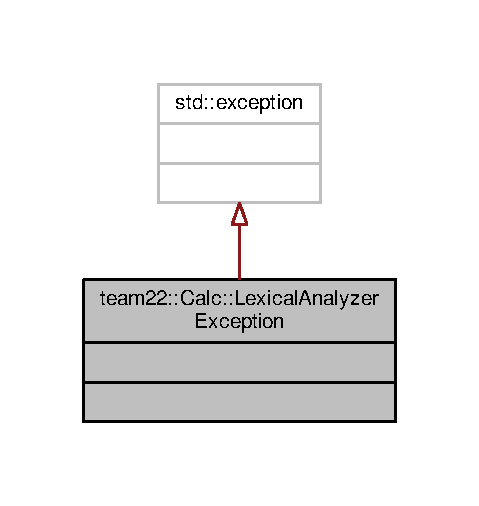
\includegraphics[width=230pt]{classteam22_1_1_calc_1_1_lexical_analyzer_exception__inherit__graph}
\end{center}
\end{figure}


Collaboration diagram for team22\+:\+:Calc\+:\+:Lexical\+Analyzer\+Exception\+:
\nopagebreak
\begin{figure}[H]
\begin{center}
\leavevmode
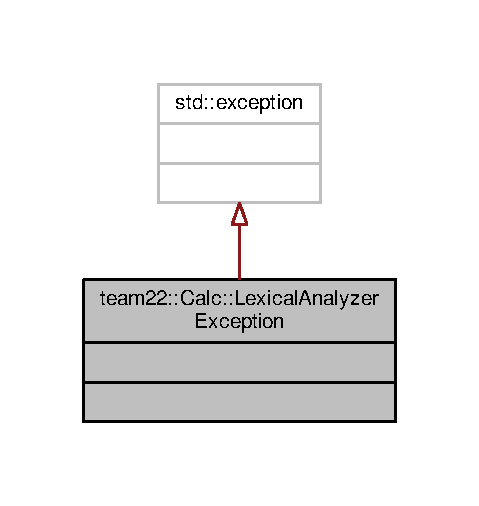
\includegraphics[width=230pt]{classteam22_1_1_calc_1_1_lexical_analyzer_exception__coll__graph}
\end{center}
\end{figure}


\subsection{Detailed Description}


Definition at line 15 of file Lexical\+Analyzer\+Exception.\+h.



The documentation for this class was generated from the following file\+:\begin{DoxyCompactItemize}
\item 
\hyperlink{_lexical_analyzer_exception_8h}{Lexical\+Analyzer\+Exception.\+h}\end{DoxyCompactItemize}

\hypertarget{struct_lexical_analyzer_test}{}\section{Lexical\+Analyzer\+Test Struct Reference}
\label{struct_lexical_analyzer_test}\index{Lexical\+Analyzer\+Test@{Lexical\+Analyzer\+Test}}


Inheritance diagram for Lexical\+Analyzer\+Test\+:
\nopagebreak
\begin{figure}[H]
\begin{center}
\leavevmode
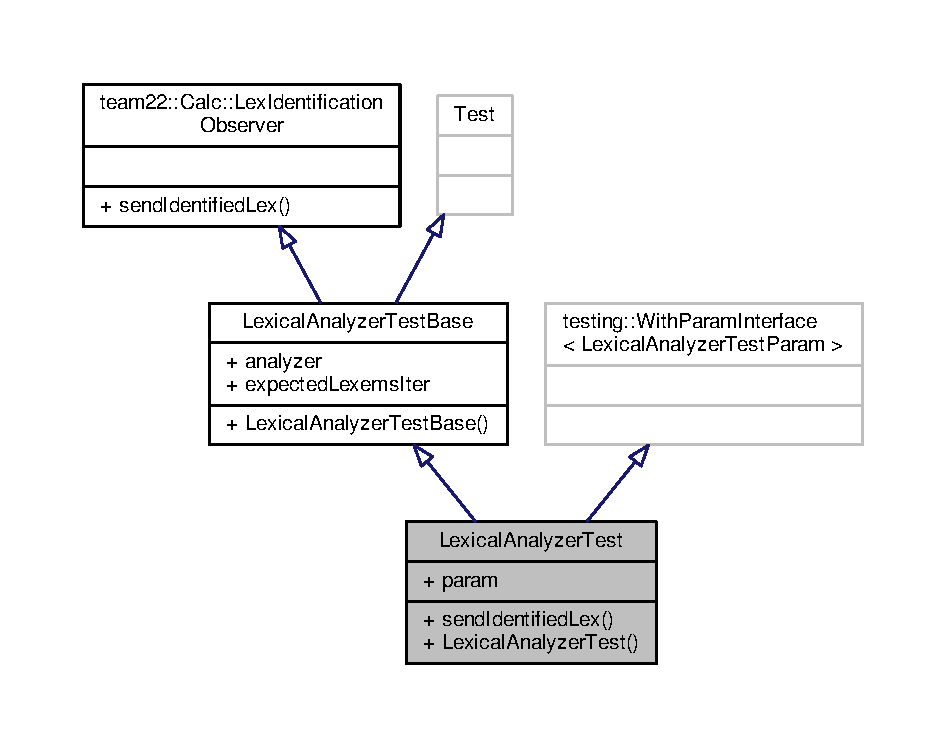
\includegraphics[width=350pt]{struct_lexical_analyzer_test__inherit__graph}
\end{center}
\end{figure}


Collaboration diagram for Lexical\+Analyzer\+Test\+:
\nopagebreak
\begin{figure}[H]
\begin{center}
\leavevmode
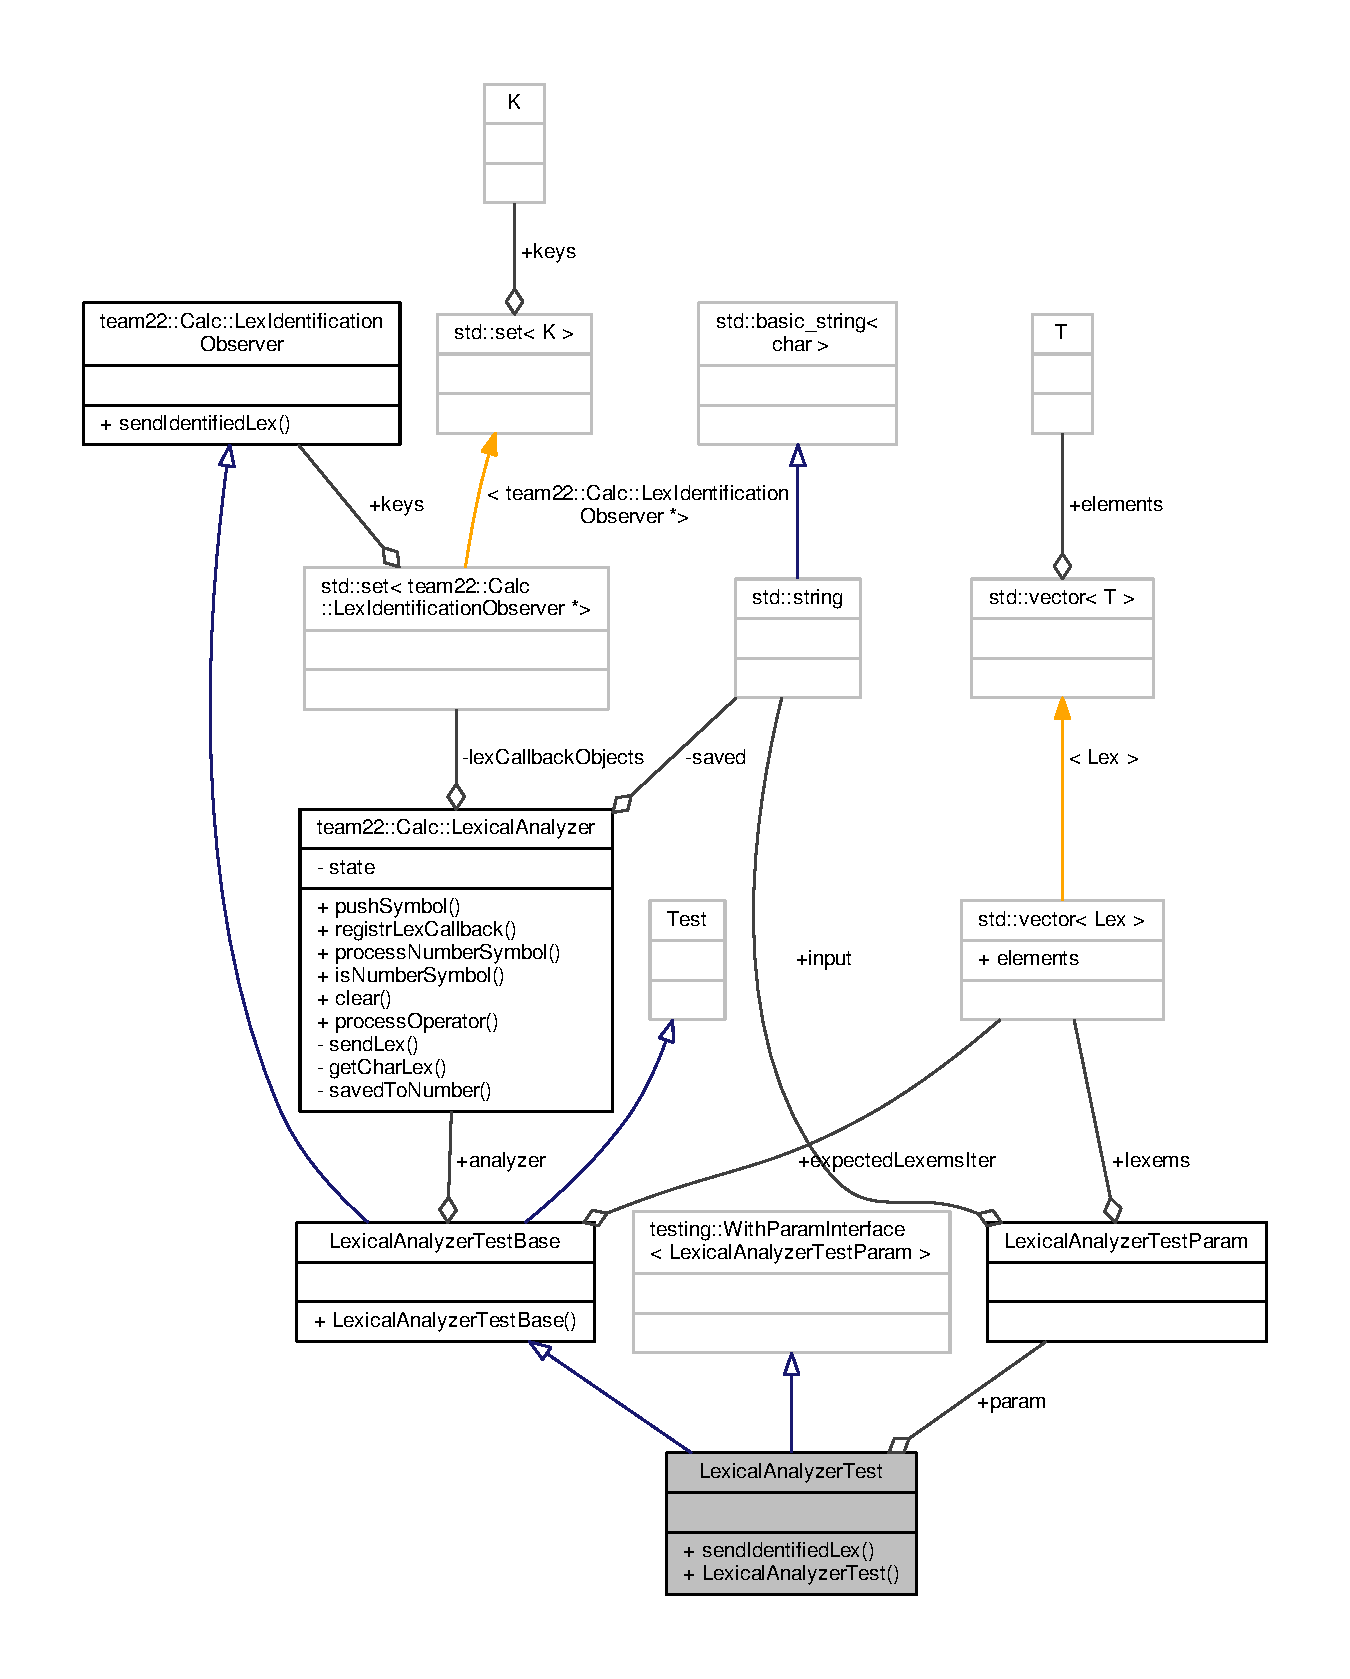
\includegraphics[width=350pt]{struct_lexical_analyzer_test__coll__graph}
\end{center}
\end{figure}
\subsection*{Public Member Functions}
\begin{DoxyCompactItemize}
\item 
void \hyperlink{struct_lexical_analyzer_test_a1c412feae956dcdc6ca0519e361e8f64}{send\+Identified\+Lex} (\hyperlink{classteam22_1_1_calc_1_1_lex}{Lex} lex) override
\item 
\hyperlink{struct_lexical_analyzer_test_a2d6000048baf250c1b0d6215f9760a92}{Lexical\+Analyzer\+Test} ()
\end{DoxyCompactItemize}
\subsection*{Public Attributes}
\begin{DoxyCompactItemize}
\item 
\hyperlink{struct_lexical_analyzer_test_param}{Lexical\+Analyzer\+Test\+Param} \hyperlink{struct_lexical_analyzer_test_ad6d61cc18154fb0f6b92eb10d840dc35}{param}
\end{DoxyCompactItemize}


\subsection{Detailed Description}


Definition at line 64 of file Lexical\+Analyzer\+Test.\+cpp.



\subsection{Constructor \& Destructor Documentation}
\mbox{\Hypertarget{struct_lexical_analyzer_test_a2d6000048baf250c1b0d6215f9760a92}\label{struct_lexical_analyzer_test_a2d6000048baf250c1b0d6215f9760a92}} 
\index{Lexical\+Analyzer\+Test@{Lexical\+Analyzer\+Test}!Lexical\+Analyzer\+Test@{Lexical\+Analyzer\+Test}}
\index{Lexical\+Analyzer\+Test@{Lexical\+Analyzer\+Test}!Lexical\+Analyzer\+Test@{Lexical\+Analyzer\+Test}}
\subsubsection{\texorpdfstring{Lexical\+Analyzer\+Test()}{LexicalAnalyzerTest()}}
{\footnotesize\ttfamily Lexical\+Analyzer\+Test\+::\+Lexical\+Analyzer\+Test (\begin{DoxyParamCaption}{ }\end{DoxyParamCaption})\hspace{0.3cm}{\ttfamily [inline]}}



Definition at line 75 of file Lexical\+Analyzer\+Test.\+cpp.



References Lexical\+Analyzer\+Test\+Param\+::lexems.



\subsection{Member Function Documentation}
\mbox{\Hypertarget{struct_lexical_analyzer_test_a1c412feae956dcdc6ca0519e361e8f64}\label{struct_lexical_analyzer_test_a1c412feae956dcdc6ca0519e361e8f64}} 
\index{Lexical\+Analyzer\+Test@{Lexical\+Analyzer\+Test}!send\+Identified\+Lex@{send\+Identified\+Lex}}
\index{send\+Identified\+Lex@{send\+Identified\+Lex}!Lexical\+Analyzer\+Test@{Lexical\+Analyzer\+Test}}
\subsubsection{\texorpdfstring{send\+Identified\+Lex()}{sendIdentifiedLex()}}
{\footnotesize\ttfamily void Lexical\+Analyzer\+Test\+::send\+Identified\+Lex (\begin{DoxyParamCaption}\item[{\hyperlink{classteam22_1_1_calc_1_1_lex}{Lex}}]{lex }\end{DoxyParamCaption})\hspace{0.3cm}{\ttfamily [inline]}, {\ttfamily [override]}, {\ttfamily [virtual]}}



Implements \hyperlink{classteam22_1_1_calc_1_1_lex_identification_observer_ac139f75c560625ec6fdb2e34cf0d4884}{team22\+::\+Calc\+::\+Lex\+Identification\+Observer}.



Definition at line 68 of file Lexical\+Analyzer\+Test.\+cpp.



\subsection{Member Data Documentation}
\mbox{\Hypertarget{struct_lexical_analyzer_test_ad6d61cc18154fb0f6b92eb10d840dc35}\label{struct_lexical_analyzer_test_ad6d61cc18154fb0f6b92eb10d840dc35}} 
\index{Lexical\+Analyzer\+Test@{Lexical\+Analyzer\+Test}!param@{param}}
\index{param@{param}!Lexical\+Analyzer\+Test@{Lexical\+Analyzer\+Test}}
\subsubsection{\texorpdfstring{param}{param}}
{\footnotesize\ttfamily \hyperlink{struct_lexical_analyzer_test_param}{Lexical\+Analyzer\+Test\+Param} Lexical\+Analyzer\+Test\+::param}



Definition at line 66 of file Lexical\+Analyzer\+Test.\+cpp.



The documentation for this struct was generated from the following file\+:\begin{DoxyCompactItemize}
\item 
src/tests/\hyperlink{_lexical_analyzer_test_8cpp}{Lexical\+Analyzer\+Test.\+cpp}\end{DoxyCompactItemize}

\hypertarget{struct_lexical_analyzer_test_base}{}\section{Lexical\+Analyzer\+Test\+Base Struct Reference}
\label{struct_lexical_analyzer_test_base}\index{Lexical\+Analyzer\+Test\+Base@{Lexical\+Analyzer\+Test\+Base}}


Inheritance diagram for Lexical\+Analyzer\+Test\+Base\+:
\nopagebreak
\begin{figure}[H]
\begin{center}
\leavevmode
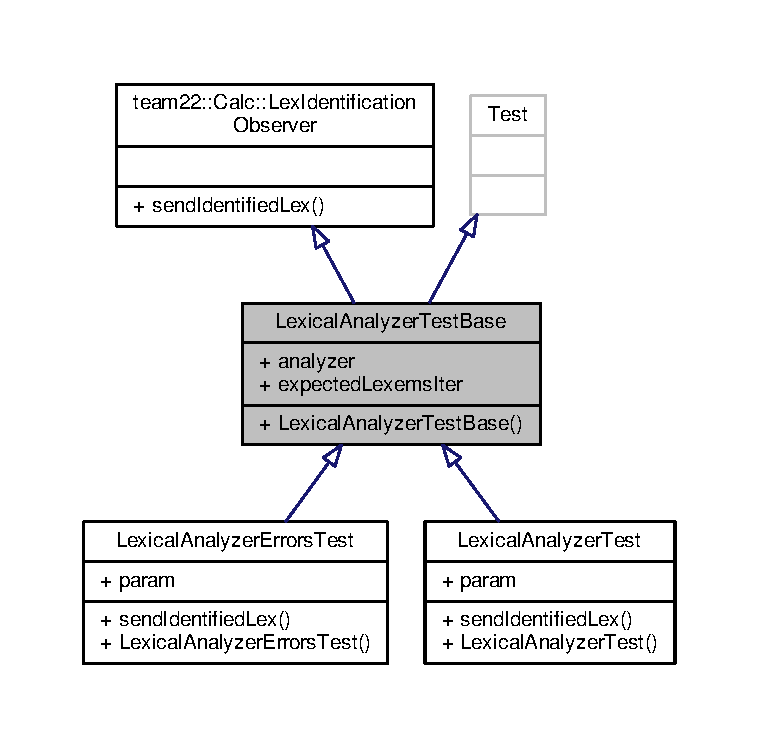
\includegraphics[width=350pt]{struct_lexical_analyzer_test_base__inherit__graph}
\end{center}
\end{figure}


Collaboration diagram for Lexical\+Analyzer\+Test\+Base\+:
\nopagebreak
\begin{figure}[H]
\begin{center}
\leavevmode
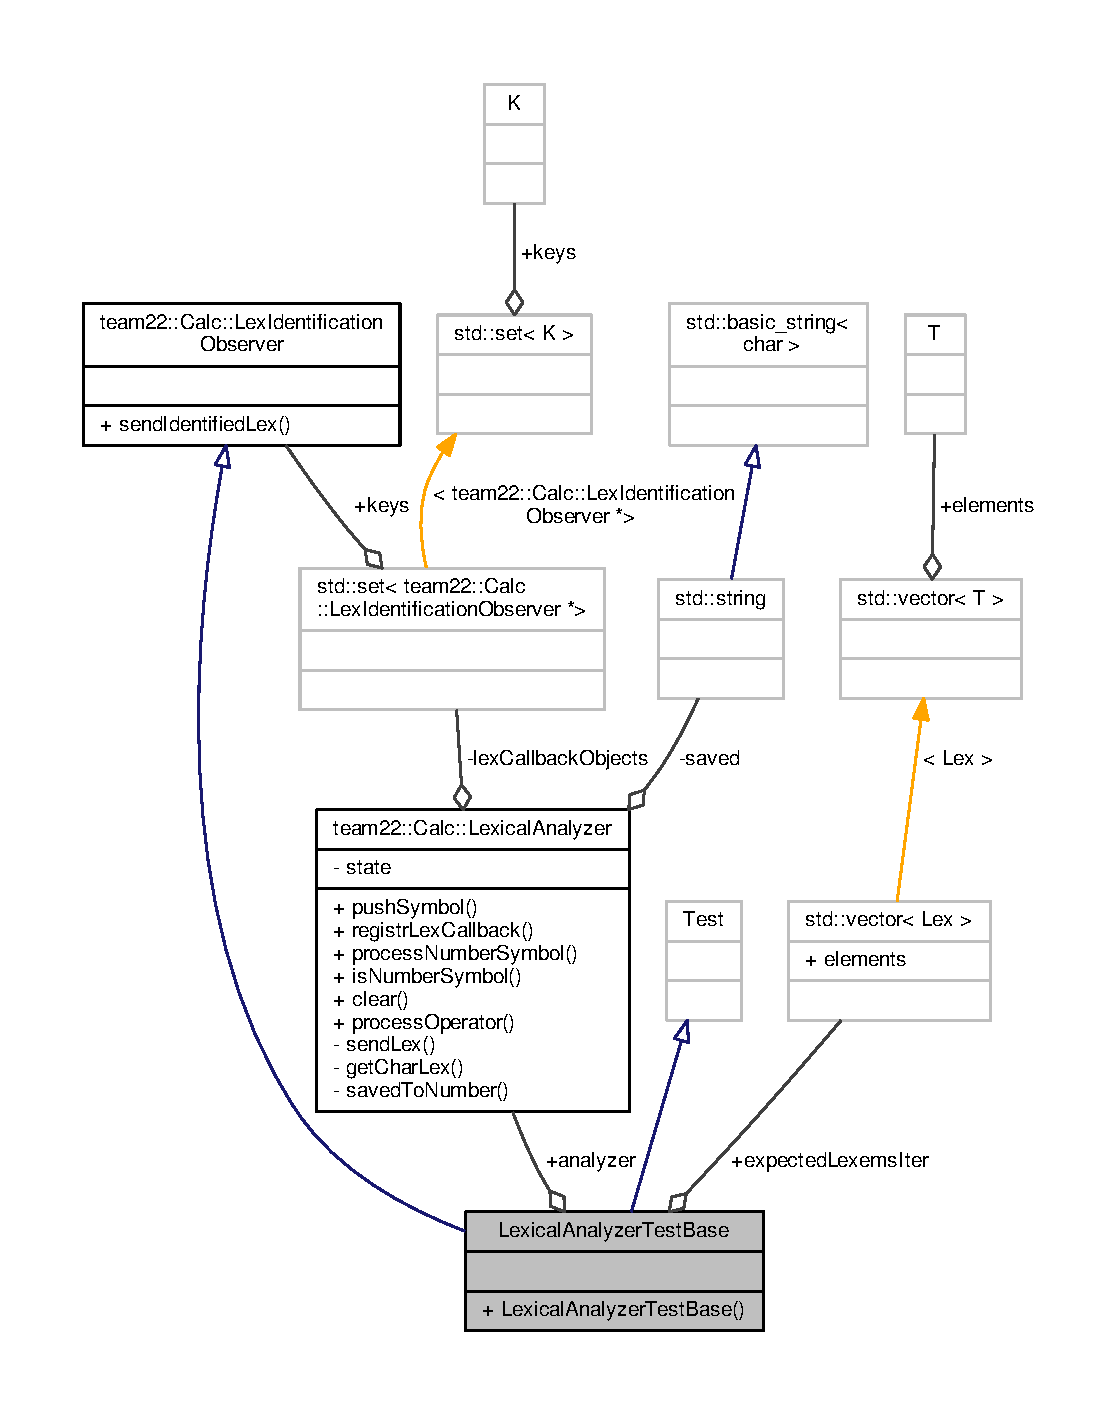
\includegraphics[width=350pt]{struct_lexical_analyzer_test_base__coll__graph}
\end{center}
\end{figure}
\subsection*{Public Member Functions}
\begin{DoxyCompactItemize}
\item 
\hyperlink{struct_lexical_analyzer_test_base_a260d79e4ec9a1b15f2c0c003ae2be078}{Lexical\+Analyzer\+Test\+Base} ()
\end{DoxyCompactItemize}
\subsection*{Public Attributes}
\begin{DoxyCompactItemize}
\item 
\hyperlink{classteam22_1_1_calc_1_1_lexical_analyzer}{Lexical\+Analyzer} \hyperlink{struct_lexical_analyzer_test_base_a4a9e40168e3b585b872642102a6dcb2b}{analyzer}
\item 
vector$<$ \hyperlink{classteam22_1_1_calc_1_1_lex}{Lex} $>$\+::iterator \hyperlink{struct_lexical_analyzer_test_base_a38cbed88c599877db18b7b7522f6b65f}{expected\+Lexems\+Iter}
\end{DoxyCompactItemize}


\subsection{Detailed Description}


Definition at line 50 of file Lexical\+Analyzer\+Test.\+cpp.



\subsection{Constructor \& Destructor Documentation}
\mbox{\Hypertarget{struct_lexical_analyzer_test_base_a260d79e4ec9a1b15f2c0c003ae2be078}\label{struct_lexical_analyzer_test_base_a260d79e4ec9a1b15f2c0c003ae2be078}} 
\index{Lexical\+Analyzer\+Test\+Base@{Lexical\+Analyzer\+Test\+Base}!Lexical\+Analyzer\+Test\+Base@{Lexical\+Analyzer\+Test\+Base}}
\index{Lexical\+Analyzer\+Test\+Base@{Lexical\+Analyzer\+Test\+Base}!Lexical\+Analyzer\+Test\+Base@{Lexical\+Analyzer\+Test\+Base}}
\subsubsection{\texorpdfstring{Lexical\+Analyzer\+Test\+Base()}{LexicalAnalyzerTestBase()}}
{\footnotesize\ttfamily Lexical\+Analyzer\+Test\+Base\+::\+Lexical\+Analyzer\+Test\+Base (\begin{DoxyParamCaption}{ }\end{DoxyParamCaption})\hspace{0.3cm}{\ttfamily [inline]}}



Definition at line 57 of file Lexical\+Analyzer\+Test.\+cpp.



References team22\+::\+Calc\+::\+Lexical\+Analyzer\+::registr\+Lex\+Callback().



\subsection{Member Data Documentation}
\mbox{\Hypertarget{struct_lexical_analyzer_test_base_a4a9e40168e3b585b872642102a6dcb2b}\label{struct_lexical_analyzer_test_base_a4a9e40168e3b585b872642102a6dcb2b}} 
\index{Lexical\+Analyzer\+Test\+Base@{Lexical\+Analyzer\+Test\+Base}!analyzer@{analyzer}}
\index{analyzer@{analyzer}!Lexical\+Analyzer\+Test\+Base@{Lexical\+Analyzer\+Test\+Base}}
\subsubsection{\texorpdfstring{analyzer}{analyzer}}
{\footnotesize\ttfamily \hyperlink{classteam22_1_1_calc_1_1_lexical_analyzer}{Lexical\+Analyzer} Lexical\+Analyzer\+Test\+Base\+::analyzer}



Definition at line 54 of file Lexical\+Analyzer\+Test.\+cpp.

\mbox{\Hypertarget{struct_lexical_analyzer_test_base_a38cbed88c599877db18b7b7522f6b65f}\label{struct_lexical_analyzer_test_base_a38cbed88c599877db18b7b7522f6b65f}} 
\index{Lexical\+Analyzer\+Test\+Base@{Lexical\+Analyzer\+Test\+Base}!expected\+Lexems\+Iter@{expected\+Lexems\+Iter}}
\index{expected\+Lexems\+Iter@{expected\+Lexems\+Iter}!Lexical\+Analyzer\+Test\+Base@{Lexical\+Analyzer\+Test\+Base}}
\subsubsection{\texorpdfstring{expected\+Lexems\+Iter}{expectedLexemsIter}}
{\footnotesize\ttfamily vector$<$\hyperlink{classteam22_1_1_calc_1_1_lex}{Lex}$>$\+::iterator Lexical\+Analyzer\+Test\+Base\+::expected\+Lexems\+Iter}



Definition at line 55 of file Lexical\+Analyzer\+Test.\+cpp.



The documentation for this struct was generated from the following file\+:\begin{DoxyCompactItemize}
\item 
src/tests/\hyperlink{_lexical_analyzer_test_8cpp}{Lexical\+Analyzer\+Test.\+cpp}\end{DoxyCompactItemize}

\hypertarget{struct_lexical_analyzer_test_param}{}\section{Lexical\+Analyzer\+Test\+Param Struct Reference}
\label{struct_lexical_analyzer_test_param}\index{Lexical\+Analyzer\+Test\+Param@{Lexical\+Analyzer\+Test\+Param}}


Collaboration diagram for Lexical\+Analyzer\+Test\+Param\+:
\nopagebreak
\begin{figure}[H]
\begin{center}
\leavevmode
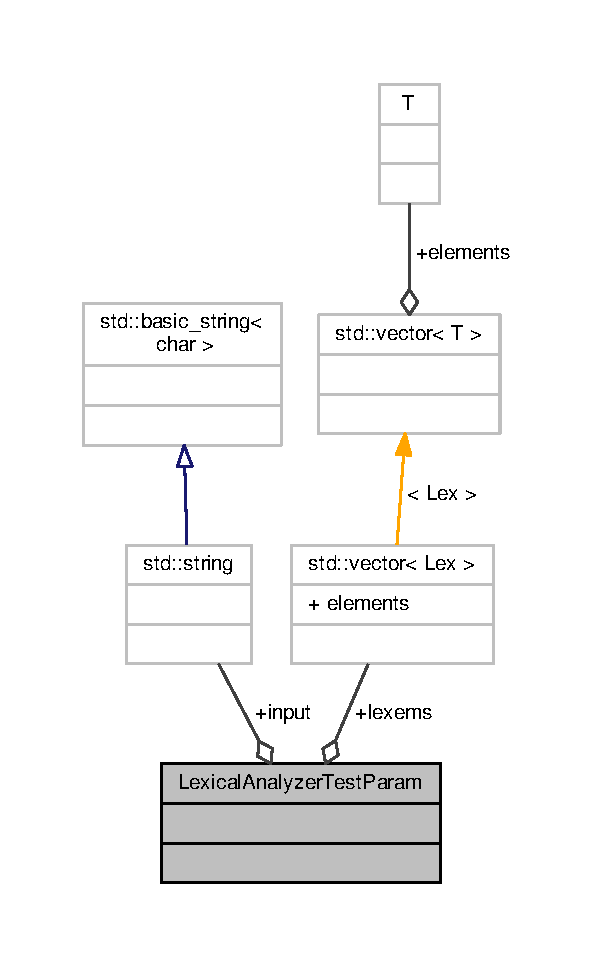
\includegraphics[width=286pt]{struct_lexical_analyzer_test_param__coll__graph}
\end{center}
\end{figure}
\subsection*{Public Attributes}
\begin{DoxyCompactItemize}
\item 
string \hyperlink{struct_lexical_analyzer_test_param_abc163995865fa8efa68a0a4dd53d77ef}{input}
\item 
vector$<$ \hyperlink{classteam22_1_1_calc_1_1_lex}{Lex} $>$ \hyperlink{struct_lexical_analyzer_test_param_a4d683034767e8307cf3bc765e40c93d8}{lexems}
\end{DoxyCompactItemize}
\subsection*{Friends}
\begin{DoxyCompactItemize}
\item 
std\+::ostream \& \hyperlink{struct_lexical_analyzer_test_param_aa38aef7ff266774e9140f334adee7200}{operator$<$$<$} (std\+::ostream \&os, const \hyperlink{struct_lexical_analyzer_test_param}{Lexical\+Analyzer\+Test\+Param} \&param)
\end{DoxyCompactItemize}


\subsection{Detailed Description}


Definition at line 23 of file Lexical\+Analyzer\+Test.\+cpp.



\subsection{Friends And Related Function Documentation}
\mbox{\Hypertarget{struct_lexical_analyzer_test_param_aa38aef7ff266774e9140f334adee7200}\label{struct_lexical_analyzer_test_param_aa38aef7ff266774e9140f334adee7200}} 
\index{Lexical\+Analyzer\+Test\+Param@{Lexical\+Analyzer\+Test\+Param}!operator$<$$<$@{operator$<$$<$}}
\index{operator$<$$<$@{operator$<$$<$}!Lexical\+Analyzer\+Test\+Param@{Lexical\+Analyzer\+Test\+Param}}
\subsubsection{\texorpdfstring{operator$<$$<$}{operator<<}}
{\footnotesize\ttfamily std\+::ostream\& operator$<$$<$ (\begin{DoxyParamCaption}\item[{std\+::ostream \&}]{os,  }\item[{const \hyperlink{struct_lexical_analyzer_test_param}{Lexical\+Analyzer\+Test\+Param} \&}]{param }\end{DoxyParamCaption})\hspace{0.3cm}{\ttfamily [friend]}}



Definition at line 27 of file Lexical\+Analyzer\+Test.\+cpp.



\subsection{Member Data Documentation}
\mbox{\Hypertarget{struct_lexical_analyzer_test_param_abc163995865fa8efa68a0a4dd53d77ef}\label{struct_lexical_analyzer_test_param_abc163995865fa8efa68a0a4dd53d77ef}} 
\index{Lexical\+Analyzer\+Test\+Param@{Lexical\+Analyzer\+Test\+Param}!input@{input}}
\index{input@{input}!Lexical\+Analyzer\+Test\+Param@{Lexical\+Analyzer\+Test\+Param}}
\subsubsection{\texorpdfstring{input}{input}}
{\footnotesize\ttfamily string Lexical\+Analyzer\+Test\+Param\+::input}



Definition at line 25 of file Lexical\+Analyzer\+Test.\+cpp.

\mbox{\Hypertarget{struct_lexical_analyzer_test_param_a4d683034767e8307cf3bc765e40c93d8}\label{struct_lexical_analyzer_test_param_a4d683034767e8307cf3bc765e40c93d8}} 
\index{Lexical\+Analyzer\+Test\+Param@{Lexical\+Analyzer\+Test\+Param}!lexems@{lexems}}
\index{lexems@{lexems}!Lexical\+Analyzer\+Test\+Param@{Lexical\+Analyzer\+Test\+Param}}
\subsubsection{\texorpdfstring{lexems}{lexems}}
{\footnotesize\ttfamily vector$<$\hyperlink{classteam22_1_1_calc_1_1_lex}{Lex}$>$ Lexical\+Analyzer\+Test\+Param\+::lexems}



Definition at line 26 of file Lexical\+Analyzer\+Test.\+cpp.



Referenced by Lexical\+Analyzer\+Test\+::\+Lexical\+Analyzer\+Test().



The documentation for this struct was generated from the following file\+:\begin{DoxyCompactItemize}
\item 
tests/\hyperlink{_lexical_analyzer_test_8cpp}{Lexical\+Analyzer\+Test.\+cpp}\end{DoxyCompactItemize}

\hypertarget{classteam22_1_1_calc_1_1_lex_identification_observer}{}\section{team22\+:\+:Calc\+:\+:Lex\+Identification\+Observer Class Reference}
\label{classteam22_1_1_calc_1_1_lex_identification_observer}\index{team22\+::\+Calc\+::\+Lex\+Identification\+Observer@{team22\+::\+Calc\+::\+Lex\+Identification\+Observer}}


{\ttfamily \#include $<$Lex\+Identification\+Observer.\+h$>$}



Inheritance diagram for team22\+:\+:Calc\+:\+:Lex\+Identification\+Observer\+:
\nopagebreak
\begin{figure}[H]
\begin{center}
\leavevmode
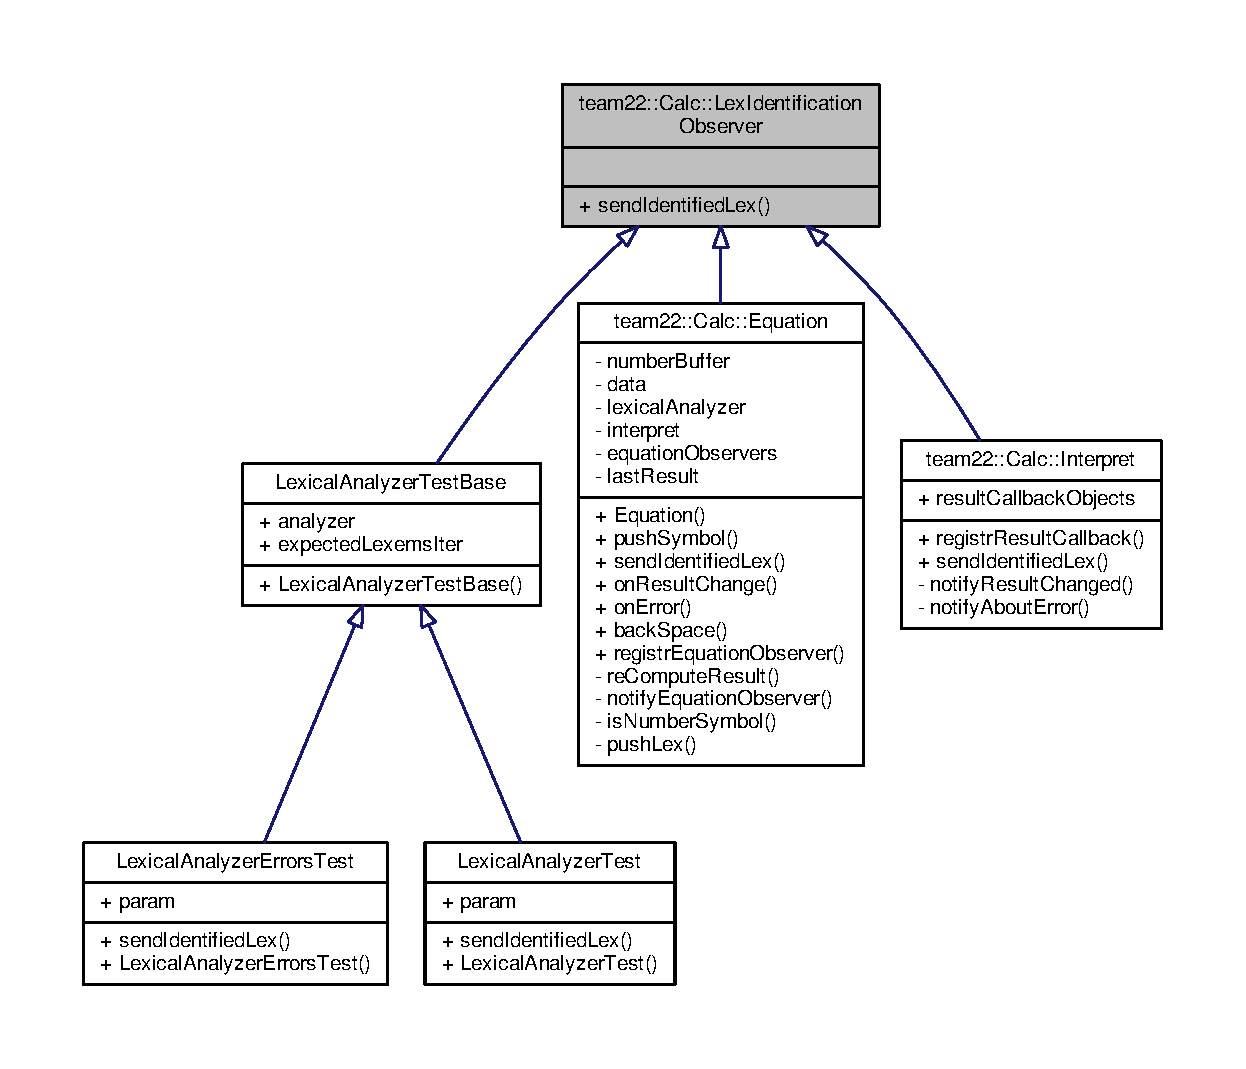
\includegraphics[width=350pt]{classteam22_1_1_calc_1_1_lex_identification_observer__inherit__graph}
\end{center}
\end{figure}


Collaboration diagram for team22\+:\+:Calc\+:\+:Lex\+Identification\+Observer\+:
\nopagebreak
\begin{figure}[H]
\begin{center}
\leavevmode
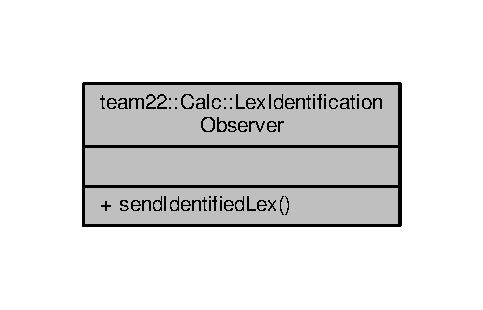
\includegraphics[width=232pt]{classteam22_1_1_calc_1_1_lex_identification_observer__coll__graph}
\end{center}
\end{figure}
\subsection*{Public Member Functions}
\begin{DoxyCompactItemize}
\item 
virtual void \hyperlink{classteam22_1_1_calc_1_1_lex_identification_observer_ac139f75c560625ec6fdb2e34cf0d4884}{send\+Identified\+Lex} (\hyperlink{classteam22_1_1_calc_1_1_lex}{Lex} lex)=0
\end{DoxyCompactItemize}


\subsection{Detailed Description}


Definition at line 15 of file Lex\+Identification\+Observer.\+h.



\subsection{Member Function Documentation}
\mbox{\Hypertarget{classteam22_1_1_calc_1_1_lex_identification_observer_ac139f75c560625ec6fdb2e34cf0d4884}\label{classteam22_1_1_calc_1_1_lex_identification_observer_ac139f75c560625ec6fdb2e34cf0d4884}} 
\index{team22\+::\+Calc\+::\+Lex\+Identification\+Observer@{team22\+::\+Calc\+::\+Lex\+Identification\+Observer}!send\+Identified\+Lex@{send\+Identified\+Lex}}
\index{send\+Identified\+Lex@{send\+Identified\+Lex}!team22\+::\+Calc\+::\+Lex\+Identification\+Observer@{team22\+::\+Calc\+::\+Lex\+Identification\+Observer}}
\subsubsection{\texorpdfstring{send\+Identified\+Lex()}{sendIdentifiedLex()}}
{\footnotesize\ttfamily virtual void team22\+::\+Calc\+::\+Lex\+Identification\+Observer\+::send\+Identified\+Lex (\begin{DoxyParamCaption}\item[{\hyperlink{classteam22_1_1_calc_1_1_lex}{Lex}}]{lex }\end{DoxyParamCaption})\hspace{0.3cm}{\ttfamily [pure virtual]}}



Implemented in \hyperlink{struct_lexical_analyzer_errors_test_ac943a4238a0eb77957e2027740603c44}{Lexical\+Analyzer\+Errors\+Test}, \hyperlink{classteam22_1_1_calc_1_1_equation_ad5768951865500ec7fc514f676de2851}{team22\+::\+Calc\+::\+Equation}, \hyperlink{classteam22_1_1_calc_1_1_interpret_a479c65c010f4ef1060049b684e5f7eb6}{team22\+::\+Calc\+::\+Interpret}, and \hyperlink{struct_lexical_analyzer_test_a1c412feae956dcdc6ca0519e361e8f64}{Lexical\+Analyzer\+Test}.



The documentation for this class was generated from the following file\+:\begin{DoxyCompactItemize}
\item 
src/\hyperlink{_lex_identification_observer_8h}{Lex\+Identification\+Observer.\+h}\end{DoxyCompactItemize}

\hypertarget{struct_mod}{}\section{Mod Struct Reference}
\label{struct_mod}\index{Mod@{Mod}}


Inheritance diagram for Mod\+:
\nopagebreak
\begin{figure}[H]
\begin{center}
\leavevmode
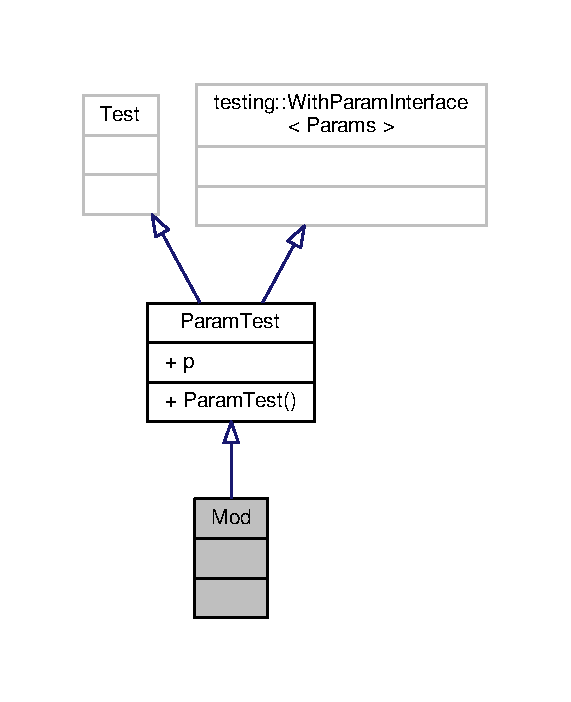
\includegraphics[width=274pt]{struct_mod__inherit__graph}
\end{center}
\end{figure}


Collaboration diagram for Mod\+:
\nopagebreak
\begin{figure}[H]
\begin{center}
\leavevmode
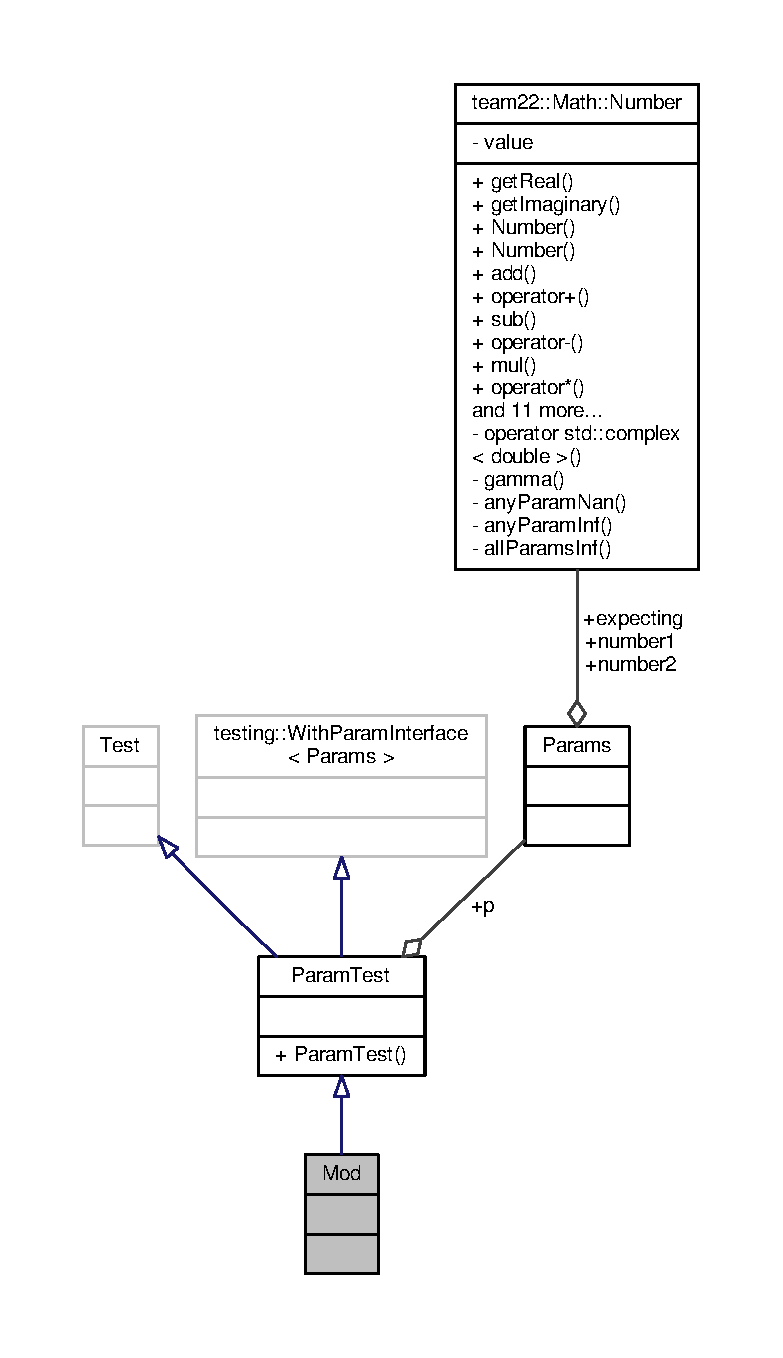
\includegraphics[height=550pt]{struct_mod__coll__graph}
\end{center}
\end{figure}
\subsection*{Additional Inherited Members}


\subsection{Detailed Description}


Definition at line 79 of file Number\+Test.\+cpp.



The documentation for this struct was generated from the following file\+:\begin{DoxyCompactItemize}
\item 
src/tests/\hyperlink{_number_test_8cpp}{Number\+Test.\+cpp}\end{DoxyCompactItemize}

\hypertarget{struct_mul}{}\section{Mul Struct Reference}
\label{struct_mul}\index{Mul@{Mul}}


Inheritance diagram for Mul\+:
\nopagebreak
\begin{figure}[H]
\begin{center}
\leavevmode
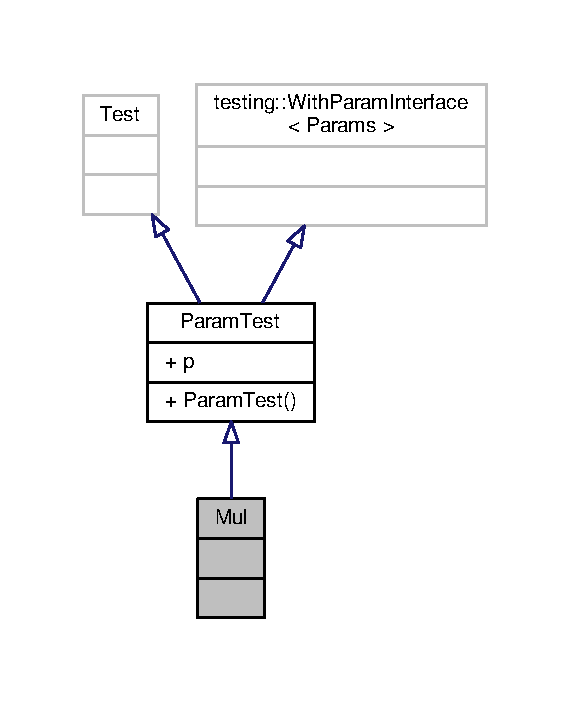
\includegraphics[width=274pt]{struct_mul__inherit__graph}
\end{center}
\end{figure}


Collaboration diagram for Mul\+:
\nopagebreak
\begin{figure}[H]
\begin{center}
\leavevmode
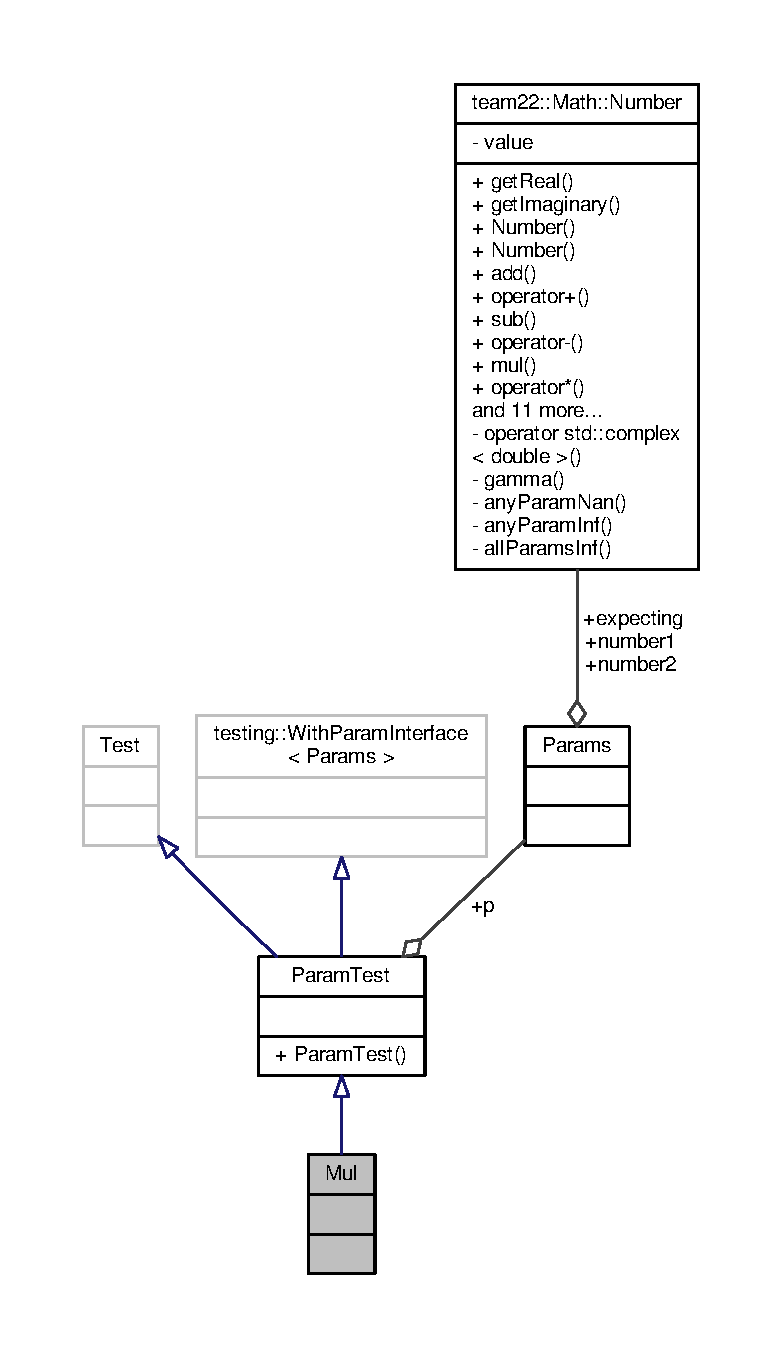
\includegraphics[height=550pt]{struct_mul__coll__graph}
\end{center}
\end{figure}
\subsection*{Additional Inherited Members}


\subsection{Detailed Description}


Definition at line 75 of file Number\+Test.\+cpp.



The documentation for this struct was generated from the following file\+:\begin{DoxyCompactItemize}
\item 
tests/\hyperlink{_number_test_8cpp}{Number\+Test.\+cpp}\end{DoxyCompactItemize}

\hypertarget{classteam22_1_1_math_1_1_number}{}\section{team22\+:\+:Math\+:\+:Number Class Reference}
\label{classteam22_1_1_math_1_1_number}\index{team22\+::\+Math\+::\+Number@{team22\+::\+Math\+::\+Number}}


{\ttfamily \#include $<$Number.\+h$>$}



Collaboration diagram for team22\+:\+:Math\+:\+:Number\+:
\nopagebreak
\begin{figure}[H]
\begin{center}
\leavevmode
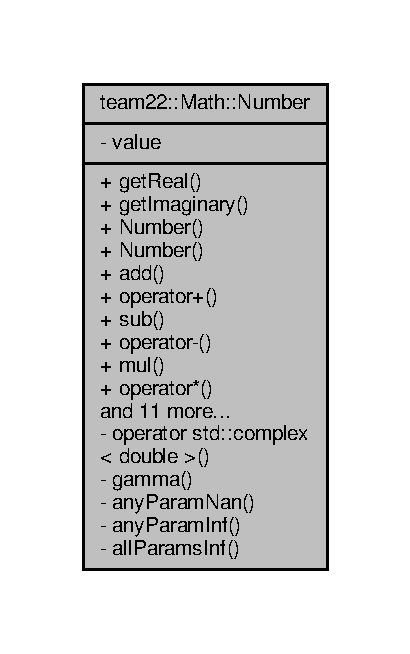
\includegraphics[width=197pt]{classteam22_1_1_math_1_1_number__coll__graph}
\end{center}
\end{figure}
\subsection*{Public Member Functions}
\begin{DoxyCompactItemize}
\item 
double \hyperlink{classteam22_1_1_math_1_1_number_adacbe355e9278da6a218598706c7f77c}{get\+Real} () const
\item 
double \hyperlink{classteam22_1_1_math_1_1_number_a033e1df614efe28459cabef254ca0a25}{get\+Imaginary} () const
\item 
\hyperlink{classteam22_1_1_math_1_1_number_a62b054aca95b93f5f36afb938223d54c}{Number} (double real, double imaginary=0)
\begin{DoxyCompactList}\small\item\em Konstruktor. \end{DoxyCompactList}\item 
\hyperlink{classteam22_1_1_math_1_1_number_a68e43ad66c5152bf7f39277bba1c0f1c}{Number} (const std\+::complex$<$ double $>$ \&other)
\begin{DoxyCompactList}\small\item\em Konstruktor. \end{DoxyCompactList}\item 
\hyperlink{classteam22_1_1_math_1_1_number}{Number} \hyperlink{classteam22_1_1_math_1_1_number_ae60b13b53c984dce975d1519e199ef8a}{add} (\hyperlink{classteam22_1_1_math_1_1_number}{Number} addend) const
\begin{DoxyCompactList}\small\item\em Sčítání \end{DoxyCompactList}\item 
\hyperlink{classteam22_1_1_math_1_1_number}{Number} \hyperlink{classteam22_1_1_math_1_1_number_abb2fc73931fb5e27e026cfedc79fdc31}{operator+} (const \hyperlink{classteam22_1_1_math_1_1_number}{Number} \&number) const
\item 
\hyperlink{classteam22_1_1_math_1_1_number}{Number} \hyperlink{classteam22_1_1_math_1_1_number_a60e8afb7de97804ac0b65bf1db37d0b4}{sub} (\hyperlink{classteam22_1_1_math_1_1_number}{Number} subtrahend) const
\begin{DoxyCompactList}\small\item\em Odečítání \end{DoxyCompactList}\item 
\hyperlink{classteam22_1_1_math_1_1_number}{Number} \hyperlink{classteam22_1_1_math_1_1_number_a5268ed342eae099e45a30541bb34e734}{operator-\/} (const \hyperlink{classteam22_1_1_math_1_1_number}{Number} \&number) const
\item 
\hyperlink{classteam22_1_1_math_1_1_number}{Number} \hyperlink{classteam22_1_1_math_1_1_number_aff9d2205901de7e4ee747de05173fb7b}{mul} (\hyperlink{classteam22_1_1_math_1_1_number}{Number} multiplier) const
\begin{DoxyCompactList}\small\item\em Násobení \end{DoxyCompactList}\item 
\hyperlink{classteam22_1_1_math_1_1_number}{Number} \hyperlink{classteam22_1_1_math_1_1_number_a0d0b4f119988b15a9b62f0886b3cf663}{operator$\ast$} (const \hyperlink{classteam22_1_1_math_1_1_number}{Number} \&number) const
\item 
\hyperlink{classteam22_1_1_math_1_1_number}{Number} \hyperlink{classteam22_1_1_math_1_1_number_a169aafbe3a08bcc9d0f8f07bee388516}{div} (\hyperlink{classteam22_1_1_math_1_1_number}{Number} divisor) const
\begin{DoxyCompactList}\small\item\em Dělení \end{DoxyCompactList}\item 
\hyperlink{classteam22_1_1_math_1_1_number}{Number} \hyperlink{classteam22_1_1_math_1_1_number_aa34d5ef75101e4b65f7840a1df0e8572}{operator/} (const \hyperlink{classteam22_1_1_math_1_1_number}{Number} \&number) const
\item 
\hyperlink{classteam22_1_1_math_1_1_number}{Number} \hyperlink{classteam22_1_1_math_1_1_number_af6d6c446579d8b8c2de69053baddd94d}{pow} (\hyperlink{classteam22_1_1_math_1_1_number}{Number} exponent) const
\begin{DoxyCompactList}\small\item\em Umocňování \end{DoxyCompactList}\item 
\hyperlink{classteam22_1_1_math_1_1_number}{Number} \hyperlink{classteam22_1_1_math_1_1_number_a7487165b416ce5db617eabb4d3415853}{operator$^\wedge$} (const \hyperlink{classteam22_1_1_math_1_1_number}{Number} \&number) const
\item 
\hyperlink{classteam22_1_1_math_1_1_number}{Number} \hyperlink{classteam22_1_1_math_1_1_number_ae2bbbafad08a50625b8070db1fc3ba98}{root} (\hyperlink{classteam22_1_1_math_1_1_number}{Number} degree) const
\begin{DoxyCompactList}\small\item\em Odmocňování \end{DoxyCompactList}\item 
\hyperlink{classteam22_1_1_math_1_1_number}{Number} \hyperlink{classteam22_1_1_math_1_1_number_a5e459d8c04e890961a71133eb53a15a9}{mod} (\hyperlink{classteam22_1_1_math_1_1_number}{Number} divisor) const
\begin{DoxyCompactList}\small\item\em Zbytek po dělení \end{DoxyCompactList}\item 
\hyperlink{classteam22_1_1_math_1_1_number}{Number} \hyperlink{classteam22_1_1_math_1_1_number_af635db4c3ad5c6818213472478a9a340}{operator\%} (const \hyperlink{classteam22_1_1_math_1_1_number}{Number} \&number) const
\item 
\hyperlink{classteam22_1_1_math_1_1_number}{Number} \hyperlink{classteam22_1_1_math_1_1_number_a79482f9f91cefb9a617e463313f4269f}{fact} ()
\begin{DoxyCompactList}\small\item\em Faktoriál. \end{DoxyCompactList}\item 
\hyperlink{classteam22_1_1_math_1_1_number}{Number} \hyperlink{classteam22_1_1_math_1_1_number_a93e5b0fdb56c604e76fa5dd28751f443}{operator!} ()
\item 
bool \hyperlink{classteam22_1_1_math_1_1_number_a91aafaa2aa878c94155e364488c56e63}{operator==} (const \hyperlink{classteam22_1_1_math_1_1_number}{Number} \&rhs) const
\item 
bool \hyperlink{classteam22_1_1_math_1_1_number_a3254778b239c52df6b311615f2cd0ad5}{operator!=} (const \hyperlink{classteam22_1_1_math_1_1_number}{Number} \&rhs) const
\end{DoxyCompactItemize}
\subsection*{Private Member Functions}
\begin{DoxyCompactItemize}
\item 
\hyperlink{classteam22_1_1_math_1_1_number_a8b38859209abab3a0a31cad9547fc77c}{operator std\+::complex$<$ double $>$} () const
\item 
std\+::complex$<$ double $>$ \hyperlink{classteam22_1_1_math_1_1_number_a614bd9dccd61f74ca50b54ebf6626ff4}{gamma} (std\+::complex$<$ double $>$ z)
\item 
bool \hyperlink{classteam22_1_1_math_1_1_number_a689b79b83d633155ac15465523634d63}{any\+Param\+Nan} (double param1, double param2, double param3, double param4) const
\item 
bool \hyperlink{classteam22_1_1_math_1_1_number_a98630956cc596c65f97ad0f24b500168}{any\+Param\+Inf} (double param1, double param2, double param3, double param4) const
\item 
bool \hyperlink{classteam22_1_1_math_1_1_number_a55293adfd56de1cac35d12878062e107}{all\+Params\+Inf} (double param1, double param2, double param3, double param4) const
\end{DoxyCompactItemize}
\subsection*{Private Attributes}
\begin{DoxyCompactItemize}
\item 
std\+::complex$<$ double $>$ \hyperlink{classteam22_1_1_math_1_1_number_a596bb514d860fbbcec3f114c3f73a59b}{value}
\end{DoxyCompactItemize}
\subsection*{Friends}
\begin{DoxyCompactItemize}
\item 
std\+::ostream \& \hyperlink{classteam22_1_1_math_1_1_number_a658f07a59742bbb5ce6432e2fd244e8b}{operator$<$$<$} (std\+::ostream \&os, const \hyperlink{classteam22_1_1_math_1_1_number}{Number} \&number)
\end{DoxyCompactItemize}


\subsection{Detailed Description}
Třída reprezentující číslo v komplexní rovině a operace nad tímto číslem 

Definition at line 24 of file Number.\+h.



\subsection{Constructor \& Destructor Documentation}
\mbox{\Hypertarget{classteam22_1_1_math_1_1_number_a62b054aca95b93f5f36afb938223d54c}\label{classteam22_1_1_math_1_1_number_a62b054aca95b93f5f36afb938223d54c}} 
\index{team22\+::\+Math\+::\+Number@{team22\+::\+Math\+::\+Number}!Number@{Number}}
\index{Number@{Number}!team22\+::\+Math\+::\+Number@{team22\+::\+Math\+::\+Number}}
\subsubsection{\texorpdfstring{Number()}{Number()}\hspace{0.1cm}{\footnotesize\ttfamily [1/2]}}
{\footnotesize\ttfamily Number\+::\+Number (\begin{DoxyParamCaption}\item[{double}]{real,  }\item[{double}]{imaginary = {\ttfamily 0} }\end{DoxyParamCaption})}



Konstruktor. 


\begin{DoxyParams}{Parameters}
{\em real} & Reálná část \\
\hline
{\em imaginary} & Imaginární část \\
\hline
\end{DoxyParams}


Definition at line 42 of file Number.\+cpp.



Referenced by operator std\+::complex$<$ double $>$().

\mbox{\Hypertarget{classteam22_1_1_math_1_1_number_a68e43ad66c5152bf7f39277bba1c0f1c}\label{classteam22_1_1_math_1_1_number_a68e43ad66c5152bf7f39277bba1c0f1c}} 
\index{team22\+::\+Math\+::\+Number@{team22\+::\+Math\+::\+Number}!Number@{Number}}
\index{Number@{Number}!team22\+::\+Math\+::\+Number@{team22\+::\+Math\+::\+Number}}
\subsubsection{\texorpdfstring{Number()}{Number()}\hspace{0.1cm}{\footnotesize\ttfamily [2/2]}}
{\footnotesize\ttfamily Number\+::\+Number (\begin{DoxyParamCaption}\item[{const std\+::complex$<$ double $>$ \&}]{other }\end{DoxyParamCaption})}



Konstruktor. 


\begin{DoxyParams}{Parameters}
{\em other} & Komplexní číslo \\
\hline
\end{DoxyParams}


Definition at line 46 of file Number.\+cpp.



\subsection{Member Function Documentation}
\mbox{\Hypertarget{classteam22_1_1_math_1_1_number_ae60b13b53c984dce975d1519e199ef8a}\label{classteam22_1_1_math_1_1_number_ae60b13b53c984dce975d1519e199ef8a}} 
\index{team22\+::\+Math\+::\+Number@{team22\+::\+Math\+::\+Number}!add@{add}}
\index{add@{add}!team22\+::\+Math\+::\+Number@{team22\+::\+Math\+::\+Number}}
\subsubsection{\texorpdfstring{add()}{add()}}
{\footnotesize\ttfamily \hyperlink{classteam22_1_1_math_1_1_number}{Number} Number\+::add (\begin{DoxyParamCaption}\item[{\hyperlink{classteam22_1_1_math_1_1_number}{Number}}]{addend }\end{DoxyParamCaption}) const}



Sčítání 


\begin{DoxyParams}{Parameters}
{\em addend} & sčítanec \\
\hline
\end{DoxyParams}
\begin{DoxyReturn}{Returns}
součet 
\end{DoxyReturn}

\begin{DoxyExceptions}{Exceptions}
{\em \hyperlink{classteam22_1_1_math_1_1_undefined_exception}{Undefined\+Exception}} & pokud je některá z částí operandů nan nebo pokud jsou obě části operandů nekonečno a zároveň operandy nejsou ze stejných kvadrantů komplexní roviny \\
\hline
\end{DoxyExceptions}


Definition at line 50 of file Number.\+cpp.



References get\+Imaginary(), and get\+Real().



Referenced by operator std\+::complex$<$ double $>$().

\mbox{\Hypertarget{classteam22_1_1_math_1_1_number_a55293adfd56de1cac35d12878062e107}\label{classteam22_1_1_math_1_1_number_a55293adfd56de1cac35d12878062e107}} 
\index{team22\+::\+Math\+::\+Number@{team22\+::\+Math\+::\+Number}!all\+Params\+Inf@{all\+Params\+Inf}}
\index{all\+Params\+Inf@{all\+Params\+Inf}!team22\+::\+Math\+::\+Number@{team22\+::\+Math\+::\+Number}}
\subsubsection{\texorpdfstring{all\+Params\+Inf()}{allParamsInf()}}
{\footnotesize\ttfamily bool Number\+::all\+Params\+Inf (\begin{DoxyParamCaption}\item[{double}]{param1,  }\item[{double}]{param2,  }\item[{double}]{param3,  }\item[{double}]{param4 }\end{DoxyParamCaption}) const\hspace{0.3cm}{\ttfamily [private]}}

\begin{DoxyReturn}{Returns}
True pokud jsou všechny parametry nekonečno, jiank False 
\end{DoxyReturn}


Definition at line 28 of file Number.\+cpp.



Referenced by operator std\+::complex$<$ double $>$().

\mbox{\Hypertarget{classteam22_1_1_math_1_1_number_a98630956cc596c65f97ad0f24b500168}\label{classteam22_1_1_math_1_1_number_a98630956cc596c65f97ad0f24b500168}} 
\index{team22\+::\+Math\+::\+Number@{team22\+::\+Math\+::\+Number}!any\+Param\+Inf@{any\+Param\+Inf}}
\index{any\+Param\+Inf@{any\+Param\+Inf}!team22\+::\+Math\+::\+Number@{team22\+::\+Math\+::\+Number}}
\subsubsection{\texorpdfstring{any\+Param\+Inf()}{anyParamInf()}}
{\footnotesize\ttfamily bool Number\+::any\+Param\+Inf (\begin{DoxyParamCaption}\item[{double}]{param1,  }\item[{double}]{param2,  }\item[{double}]{param3,  }\item[{double}]{param4 }\end{DoxyParamCaption}) const\hspace{0.3cm}{\ttfamily [private]}}

\begin{DoxyReturn}{Returns}
True pokud je některý z parametrů nekonečno, jiank False 
\end{DoxyReturn}


Definition at line 22 of file Number.\+cpp.



Referenced by operator std\+::complex$<$ double $>$().

\mbox{\Hypertarget{classteam22_1_1_math_1_1_number_a689b79b83d633155ac15465523634d63}\label{classteam22_1_1_math_1_1_number_a689b79b83d633155ac15465523634d63}} 
\index{team22\+::\+Math\+::\+Number@{team22\+::\+Math\+::\+Number}!any\+Param\+Nan@{any\+Param\+Nan}}
\index{any\+Param\+Nan@{any\+Param\+Nan}!team22\+::\+Math\+::\+Number@{team22\+::\+Math\+::\+Number}}
\subsubsection{\texorpdfstring{any\+Param\+Nan()}{anyParamNan()}}
{\footnotesize\ttfamily bool Number\+::any\+Param\+Nan (\begin{DoxyParamCaption}\item[{double}]{param1,  }\item[{double}]{param2,  }\item[{double}]{param3,  }\item[{double}]{param4 }\end{DoxyParamCaption}) const\hspace{0.3cm}{\ttfamily [private]}}

\begin{DoxyReturn}{Returns}
True pokud je některý z parametrů Nan, jiank False 
\end{DoxyReturn}


Definition at line 16 of file Number.\+cpp.



Referenced by operator std\+::complex$<$ double $>$().

\mbox{\Hypertarget{classteam22_1_1_math_1_1_number_a169aafbe3a08bcc9d0f8f07bee388516}\label{classteam22_1_1_math_1_1_number_a169aafbe3a08bcc9d0f8f07bee388516}} 
\index{team22\+::\+Math\+::\+Number@{team22\+::\+Math\+::\+Number}!div@{div}}
\index{div@{div}!team22\+::\+Math\+::\+Number@{team22\+::\+Math\+::\+Number}}
\subsubsection{\texorpdfstring{div()}{div()}}
{\footnotesize\ttfamily \hyperlink{classteam22_1_1_math_1_1_number}{Number} Number\+::div (\begin{DoxyParamCaption}\item[{\hyperlink{classteam22_1_1_math_1_1_number}{Number}}]{divisor }\end{DoxyParamCaption}) const}



Dělení 


\begin{DoxyParams}{Parameters}
{\em divisor} & dělitel \\
\hline
\end{DoxyParams}
\begin{DoxyReturn}{Returns}
rozdíl 
\end{DoxyReturn}

\begin{DoxyExceptions}{Exceptions}
{\em \hyperlink{classteam22_1_1_math_1_1_undefined_exception}{Undefined\+Exception}} & Pokud je některá část operandů nan nebo obě části obou operandů jsou nekonečno nebo je dělitel nulový a obě části dělence nejsou nekonečno a reálná část dělence není pozitivní nekonečno a imaginární část dělence není nekonečno \\
\hline
\end{DoxyExceptions}


Definition at line 96 of file Number.\+cpp.



References get\+Imaginary(), and get\+Real().



Referenced by operator std\+::complex$<$ double $>$().

\mbox{\Hypertarget{classteam22_1_1_math_1_1_number_a79482f9f91cefb9a617e463313f4269f}\label{classteam22_1_1_math_1_1_number_a79482f9f91cefb9a617e463313f4269f}} 
\index{team22\+::\+Math\+::\+Number@{team22\+::\+Math\+::\+Number}!fact@{fact}}
\index{fact@{fact}!team22\+::\+Math\+::\+Number@{team22\+::\+Math\+::\+Number}}
\subsubsection{\texorpdfstring{fact()}{fact()}}
{\footnotesize\ttfamily \hyperlink{classteam22_1_1_math_1_1_number}{Number} Number\+::fact (\begin{DoxyParamCaption}{ }\end{DoxyParamCaption})}



Faktoriál. 

\begin{DoxyReturn}{Returns}
faktoriál 
\end{DoxyReturn}

\begin{DoxyExceptions}{Exceptions}
{\em \hyperlink{classteam22_1_1_math_1_1_undefined_exception}{Undefined\+Exception}} & pokud je některá z částí operandů nan nebo jsou obě části operandů nekonečno nebo je reálná část operandu záporné nekonečno \\
\hline
\end{DoxyExceptions}


Definition at line 181 of file Number.\+cpp.



Referenced by operator std\+::complex$<$ double $>$().

\mbox{\Hypertarget{classteam22_1_1_math_1_1_number_a614bd9dccd61f74ca50b54ebf6626ff4}\label{classteam22_1_1_math_1_1_number_a614bd9dccd61f74ca50b54ebf6626ff4}} 
\index{team22\+::\+Math\+::\+Number@{team22\+::\+Math\+::\+Number}!gamma@{gamma}}
\index{gamma@{gamma}!team22\+::\+Math\+::\+Number@{team22\+::\+Math\+::\+Number}}
\subsubsection{\texorpdfstring{gamma()}{gamma()}}
{\footnotesize\ttfamily complex$<$ double $>$ Number\+::gamma (\begin{DoxyParamCaption}\item[{std\+::complex$<$ double $>$}]{z }\end{DoxyParamCaption})\hspace{0.3cm}{\ttfamily [private]}}

Gamma funkce implementovaná pomocí Lanczosovy aproximace


\begin{DoxyParams}{Parameters}
{\em z} & vstupní operand \\
\hline
\end{DoxyParams}
\begin{DoxyReturn}{Returns}
gamma čísla z 
\end{DoxyReturn}


Definition at line 224 of file Number.\+cpp.



References c, get\+Imaginary(), and get\+Real().



Referenced by operator std\+::complex$<$ double $>$().

\mbox{\Hypertarget{classteam22_1_1_math_1_1_number_a033e1df614efe28459cabef254ca0a25}\label{classteam22_1_1_math_1_1_number_a033e1df614efe28459cabef254ca0a25}} 
\index{team22\+::\+Math\+::\+Number@{team22\+::\+Math\+::\+Number}!get\+Imaginary@{get\+Imaginary}}
\index{get\+Imaginary@{get\+Imaginary}!team22\+::\+Math\+::\+Number@{team22\+::\+Math\+::\+Number}}
\subsubsection{\texorpdfstring{get\+Imaginary()}{getImaginary()}}
{\footnotesize\ttfamily double Number\+::get\+Imaginary (\begin{DoxyParamCaption}{ }\end{DoxyParamCaption}) const}

Imaginární část \begin{DoxyReturn}{Returns}

\end{DoxyReturn}


Definition at line 38 of file Number.\+cpp.



Referenced by add(), div(), gamma(), mod(), mul(), operator std\+::complex$<$ double $>$(), pow(), root(), and sub().

\mbox{\Hypertarget{classteam22_1_1_math_1_1_number_adacbe355e9278da6a218598706c7f77c}\label{classteam22_1_1_math_1_1_number_adacbe355e9278da6a218598706c7f77c}} 
\index{team22\+::\+Math\+::\+Number@{team22\+::\+Math\+::\+Number}!get\+Real@{get\+Real}}
\index{get\+Real@{get\+Real}!team22\+::\+Math\+::\+Number@{team22\+::\+Math\+::\+Number}}
\subsubsection{\texorpdfstring{get\+Real()}{getReal()}}
{\footnotesize\ttfamily double Number\+::get\+Real (\begin{DoxyParamCaption}{ }\end{DoxyParamCaption}) const}

Realná část \begin{DoxyReturn}{Returns}

\end{DoxyReturn}


Definition at line 34 of file Number.\+cpp.



Referenced by add(), div(), gamma(), mod(), mul(), operator std\+::complex$<$ double $>$(), pow(), root(), and sub().

\mbox{\Hypertarget{classteam22_1_1_math_1_1_number_a5e459d8c04e890961a71133eb53a15a9}\label{classteam22_1_1_math_1_1_number_a5e459d8c04e890961a71133eb53a15a9}} 
\index{team22\+::\+Math\+::\+Number@{team22\+::\+Math\+::\+Number}!mod@{mod}}
\index{mod@{mod}!team22\+::\+Math\+::\+Number@{team22\+::\+Math\+::\+Number}}
\subsubsection{\texorpdfstring{mod()}{mod()}}
{\footnotesize\ttfamily \hyperlink{classteam22_1_1_math_1_1_number}{Number} Number\+::mod (\begin{DoxyParamCaption}\item[{\hyperlink{classteam22_1_1_math_1_1_number}{Number}}]{divisor }\end{DoxyParamCaption}) const}



Zbytek po dělení 


\begin{DoxyParams}{Parameters}
{\em divisor} & dělitel \\
\hline
\end{DoxyParams}
\begin{DoxyReturn}{Returns}
zbytek 
\end{DoxyReturn}

\begin{DoxyExceptions}{Exceptions}
{\em \hyperlink{classteam22_1_1_math_1_1_undefined_exception}{Undefined\+Exception}} & pokud je některá z částí operandů nan nebo nekonečno nebo pokud je dělitel nulový \\
\hline
\end{DoxyExceptions}


Definition at line 160 of file Number.\+cpp.



References get\+Imaginary(), and get\+Real().



Referenced by operator std\+::complex$<$ double $>$().

\mbox{\Hypertarget{classteam22_1_1_math_1_1_number_aff9d2205901de7e4ee747de05173fb7b}\label{classteam22_1_1_math_1_1_number_aff9d2205901de7e4ee747de05173fb7b}} 
\index{team22\+::\+Math\+::\+Number@{team22\+::\+Math\+::\+Number}!mul@{mul}}
\index{mul@{mul}!team22\+::\+Math\+::\+Number@{team22\+::\+Math\+::\+Number}}
\subsubsection{\texorpdfstring{mul()}{mul()}}
{\footnotesize\ttfamily \hyperlink{classteam22_1_1_math_1_1_number}{Number} Number\+::mul (\begin{DoxyParamCaption}\item[{\hyperlink{classteam22_1_1_math_1_1_number}{Number}}]{multiplier }\end{DoxyParamCaption}) const}



Násobení 


\begin{DoxyParams}{Parameters}
{\em multiplier} & činitel \\
\hline
\end{DoxyParams}
\begin{DoxyReturn}{Returns}
součin 
\end{DoxyReturn}

\begin{DoxyExceptions}{Exceptions}
{\em \hyperlink{classteam22_1_1_math_1_1_undefined_exception}{Undefined\+Exception}} & pokud je některá z částí operandů nan nebo nekonečno \\
\hline
\end{DoxyExceptions}


Definition at line 82 of file Number.\+cpp.



References get\+Imaginary(), and get\+Real().



Referenced by operator std\+::complex$<$ double $>$().

\mbox{\Hypertarget{classteam22_1_1_math_1_1_number_a8b38859209abab3a0a31cad9547fc77c}\label{classteam22_1_1_math_1_1_number_a8b38859209abab3a0a31cad9547fc77c}} 
\index{team22\+::\+Math\+::\+Number@{team22\+::\+Math\+::\+Number}!operator std\+::complex$<$ double $>$@{operator std\+::complex$<$ double $>$}}
\index{operator std\+::complex$<$ double $>$@{operator std\+::complex$<$ double $>$}!team22\+::\+Math\+::\+Number@{team22\+::\+Math\+::\+Number}}
\subsubsection{\texorpdfstring{operator std\+::complex$<$ double $>$()}{operator std::complex< double >()}}
{\footnotesize\ttfamily team22\+::\+Math\+::\+Number\+::operator std\+::complex$<$ double $>$ (\begin{DoxyParamCaption}{ }\end{DoxyParamCaption}) const\hspace{0.3cm}{\ttfamily [inline]}, {\ttfamily [explicit]}, {\ttfamily [private]}}



Definition at line 30 of file Number.\+h.



References add(), all\+Params\+Inf(), any\+Param\+Inf(), any\+Param\+Nan(), div(), fact(), gamma(), get\+Imaginary(), get\+Real(), mod(), mul(), Number(), operator!(), operator!=(), operator\%(), operator$\ast$(), operator+(), operator-\/(), operator/(), operator$<$$<$, operator==(), operator$^\wedge$(), pow(), root(), sub(), and value.

\mbox{\Hypertarget{classteam22_1_1_math_1_1_number_a93e5b0fdb56c604e76fa5dd28751f443}\label{classteam22_1_1_math_1_1_number_a93e5b0fdb56c604e76fa5dd28751f443}} 
\index{team22\+::\+Math\+::\+Number@{team22\+::\+Math\+::\+Number}!operator"!@{operator"!}}
\index{operator"!@{operator"!}!team22\+::\+Math\+::\+Number@{team22\+::\+Math\+::\+Number}}
\subsubsection{\texorpdfstring{operator"!()}{operator!()}}
{\footnotesize\ttfamily \hyperlink{classteam22_1_1_math_1_1_number}{Number} Number\+::operator! (\begin{DoxyParamCaption}{ }\end{DoxyParamCaption})}

\begin{DoxySeeAlso}{See also}
\+::fact 
\end{DoxySeeAlso}


Definition at line 204 of file Number.\+cpp.



Referenced by operator std\+::complex$<$ double $>$().

\mbox{\Hypertarget{classteam22_1_1_math_1_1_number_a3254778b239c52df6b311615f2cd0ad5}\label{classteam22_1_1_math_1_1_number_a3254778b239c52df6b311615f2cd0ad5}} 
\index{team22\+::\+Math\+::\+Number@{team22\+::\+Math\+::\+Number}!operator"!=@{operator"!=}}
\index{operator"!=@{operator"!=}!team22\+::\+Math\+::\+Number@{team22\+::\+Math\+::\+Number}}
\subsubsection{\texorpdfstring{operator"!=()}{operator!=()}}
{\footnotesize\ttfamily bool \hyperlink{classteam22_1_1_math_1_1_number_a93e5b0fdb56c604e76fa5dd28751f443}{team22\+::\+Math\+::\+Number\+::operator!}= (\begin{DoxyParamCaption}\item[{const \hyperlink{classteam22_1_1_math_1_1_number}{Number} \&}]{rhs }\end{DoxyParamCaption}) const}



Definition at line 263 of file Number.\+cpp.



Referenced by operator std\+::complex$<$ double $>$().

\mbox{\Hypertarget{classteam22_1_1_math_1_1_number_af635db4c3ad5c6818213472478a9a340}\label{classteam22_1_1_math_1_1_number_af635db4c3ad5c6818213472478a9a340}} 
\index{team22\+::\+Math\+::\+Number@{team22\+::\+Math\+::\+Number}!operator\%@{operator\%}}
\index{operator\%@{operator\%}!team22\+::\+Math\+::\+Number@{team22\+::\+Math\+::\+Number}}
\subsubsection{\texorpdfstring{operator\%()}{operator\%()}}
{\footnotesize\ttfamily \hyperlink{classteam22_1_1_math_1_1_number}{Number} Number\+::operator\% (\begin{DoxyParamCaption}\item[{const \hyperlink{classteam22_1_1_math_1_1_number}{Number} \&}]{number }\end{DoxyParamCaption}) const}

\begin{DoxySeeAlso}{See also}
\+::mod 
\end{DoxySeeAlso}


Definition at line 177 of file Number.\+cpp.



Referenced by operator std\+::complex$<$ double $>$().

\mbox{\Hypertarget{classteam22_1_1_math_1_1_number_a0d0b4f119988b15a9b62f0886b3cf663}\label{classteam22_1_1_math_1_1_number_a0d0b4f119988b15a9b62f0886b3cf663}} 
\index{team22\+::\+Math\+::\+Number@{team22\+::\+Math\+::\+Number}!operator$\ast$@{operator$\ast$}}
\index{operator$\ast$@{operator$\ast$}!team22\+::\+Math\+::\+Number@{team22\+::\+Math\+::\+Number}}
\subsubsection{\texorpdfstring{operator$\ast$()}{operator*()}}
{\footnotesize\ttfamily \hyperlink{classteam22_1_1_math_1_1_number}{Number} Number\+::operator$\ast$ (\begin{DoxyParamCaption}\item[{const \hyperlink{classteam22_1_1_math_1_1_number}{Number} \&}]{number }\end{DoxyParamCaption}) const}

\begin{DoxySeeAlso}{See also}
\+::mul 
\end{DoxySeeAlso}


Definition at line 92 of file Number.\+cpp.



Referenced by operator std\+::complex$<$ double $>$().

\mbox{\Hypertarget{classteam22_1_1_math_1_1_number_abb2fc73931fb5e27e026cfedc79fdc31}\label{classteam22_1_1_math_1_1_number_abb2fc73931fb5e27e026cfedc79fdc31}} 
\index{team22\+::\+Math\+::\+Number@{team22\+::\+Math\+::\+Number}!operator+@{operator+}}
\index{operator+@{operator+}!team22\+::\+Math\+::\+Number@{team22\+::\+Math\+::\+Number}}
\subsubsection{\texorpdfstring{operator+()}{operator+()}}
{\footnotesize\ttfamily \hyperlink{classteam22_1_1_math_1_1_number}{Number} Number\+::operator+ (\begin{DoxyParamCaption}\item[{const \hyperlink{classteam22_1_1_math_1_1_number}{Number} \&}]{number }\end{DoxyParamCaption}) const}

\begin{DoxySeeAlso}{See also}
\+::add 
\end{DoxySeeAlso}


Definition at line 62 of file Number.\+cpp.



Referenced by operator std\+::complex$<$ double $>$().

\mbox{\Hypertarget{classteam22_1_1_math_1_1_number_a5268ed342eae099e45a30541bb34e734}\label{classteam22_1_1_math_1_1_number_a5268ed342eae099e45a30541bb34e734}} 
\index{team22\+::\+Math\+::\+Number@{team22\+::\+Math\+::\+Number}!operator-\/@{operator-\/}}
\index{operator-\/@{operator-\/}!team22\+::\+Math\+::\+Number@{team22\+::\+Math\+::\+Number}}
\subsubsection{\texorpdfstring{operator-\/()}{operator-()}}
{\footnotesize\ttfamily \hyperlink{classteam22_1_1_math_1_1_number}{Number} Number\+::operator-\/ (\begin{DoxyParamCaption}\item[{const \hyperlink{classteam22_1_1_math_1_1_number}{Number} \&}]{number }\end{DoxyParamCaption}) const}

\begin{DoxySeeAlso}{See also}
\+::sub 
\end{DoxySeeAlso}


Definition at line 78 of file Number.\+cpp.



Referenced by operator std\+::complex$<$ double $>$().

\mbox{\Hypertarget{classteam22_1_1_math_1_1_number_aa34d5ef75101e4b65f7840a1df0e8572}\label{classteam22_1_1_math_1_1_number_aa34d5ef75101e4b65f7840a1df0e8572}} 
\index{team22\+::\+Math\+::\+Number@{team22\+::\+Math\+::\+Number}!operator/@{operator/}}
\index{operator/@{operator/}!team22\+::\+Math\+::\+Number@{team22\+::\+Math\+::\+Number}}
\subsubsection{\texorpdfstring{operator/()}{operator/()}}
{\footnotesize\ttfamily \hyperlink{classteam22_1_1_math_1_1_number}{Number} Number\+::operator/ (\begin{DoxyParamCaption}\item[{const \hyperlink{classteam22_1_1_math_1_1_number}{Number} \&}]{number }\end{DoxyParamCaption}) const}

\begin{DoxySeeAlso}{See also}
\+::div 
\end{DoxySeeAlso}


Definition at line 113 of file Number.\+cpp.



Referenced by operator std\+::complex$<$ double $>$().

\mbox{\Hypertarget{classteam22_1_1_math_1_1_number_a91aafaa2aa878c94155e364488c56e63}\label{classteam22_1_1_math_1_1_number_a91aafaa2aa878c94155e364488c56e63}} 
\index{team22\+::\+Math\+::\+Number@{team22\+::\+Math\+::\+Number}!operator==@{operator==}}
\index{operator==@{operator==}!team22\+::\+Math\+::\+Number@{team22\+::\+Math\+::\+Number}}
\subsubsection{\texorpdfstring{operator==()}{operator==()}}
{\footnotesize\ttfamily bool team22\+::\+Math\+::\+Number\+::operator== (\begin{DoxyParamCaption}\item[{const \hyperlink{classteam22_1_1_math_1_1_number}{Number} \&}]{rhs }\end{DoxyParamCaption}) const}



Definition at line 258 of file Number.\+cpp.



References value.



Referenced by operator std\+::complex$<$ double $>$().

\mbox{\Hypertarget{classteam22_1_1_math_1_1_number_a7487165b416ce5db617eabb4d3415853}\label{classteam22_1_1_math_1_1_number_a7487165b416ce5db617eabb4d3415853}} 
\index{team22\+::\+Math\+::\+Number@{team22\+::\+Math\+::\+Number}!operator$^\wedge$@{operator$^\wedge$}}
\index{operator$^\wedge$@{operator$^\wedge$}!team22\+::\+Math\+::\+Number@{team22\+::\+Math\+::\+Number}}
\subsubsection{\texorpdfstring{operator$^\wedge$()}{operator^()}}
{\footnotesize\ttfamily \hyperlink{classteam22_1_1_math_1_1_number}{Number} Number\+::operator$^\wedge$ (\begin{DoxyParamCaption}\item[{const \hyperlink{classteam22_1_1_math_1_1_number}{Number} \&}]{number }\end{DoxyParamCaption}) const}

\begin{DoxySeeAlso}{See also}
\+::pow 
\end{DoxySeeAlso}


Definition at line 137 of file Number.\+cpp.



Referenced by operator std\+::complex$<$ double $>$().

\mbox{\Hypertarget{classteam22_1_1_math_1_1_number_af6d6c446579d8b8c2de69053baddd94d}\label{classteam22_1_1_math_1_1_number_af6d6c446579d8b8c2de69053baddd94d}} 
\index{team22\+::\+Math\+::\+Number@{team22\+::\+Math\+::\+Number}!pow@{pow}}
\index{pow@{pow}!team22\+::\+Math\+::\+Number@{team22\+::\+Math\+::\+Number}}
\subsubsection{\texorpdfstring{pow()}{pow()}}
{\footnotesize\ttfamily \hyperlink{classteam22_1_1_math_1_1_number}{Number} Number\+::pow (\begin{DoxyParamCaption}\item[{\hyperlink{classteam22_1_1_math_1_1_number}{Number}}]{exponent }\end{DoxyParamCaption}) const}



Umocňování 


\begin{DoxyParams}{Parameters}
{\em exponent} & mocnitel \\
\hline
\end{DoxyParams}
\begin{DoxyReturn}{Returns}
mocnina 
\end{DoxyReturn}

\begin{DoxyExceptions}{Exceptions}
{\em \hyperlink{classteam22_1_1_math_1_1_undefined_exception}{Undefined\+Exception}} & T\+O\+DO \\
\hline
\end{DoxyExceptions}


Definition at line 117 of file Number.\+cpp.



References get\+Imaginary(), and get\+Real().



Referenced by operator std\+::complex$<$ double $>$().

\mbox{\Hypertarget{classteam22_1_1_math_1_1_number_ae2bbbafad08a50625b8070db1fc3ba98}\label{classteam22_1_1_math_1_1_number_ae2bbbafad08a50625b8070db1fc3ba98}} 
\index{team22\+::\+Math\+::\+Number@{team22\+::\+Math\+::\+Number}!root@{root}}
\index{root@{root}!team22\+::\+Math\+::\+Number@{team22\+::\+Math\+::\+Number}}
\subsubsection{\texorpdfstring{root()}{root()}}
{\footnotesize\ttfamily \hyperlink{classteam22_1_1_math_1_1_number}{Number} Number\+::root (\begin{DoxyParamCaption}\item[{\hyperlink{classteam22_1_1_math_1_1_number}{Number}}]{degree }\end{DoxyParamCaption}) const}



Odmocňování 


\begin{DoxyParams}{Parameters}
{\em degree} & odmocnitel \\
\hline
\end{DoxyParams}
\begin{DoxyReturn}{Returns}
odmocnina 
\end{DoxyReturn}

\begin{DoxyExceptions}{Exceptions}
{\em \hyperlink{classteam22_1_1_math_1_1_undefined_exception}{Undefined\+Exception}} & pokud je některá z částí operandů nan nebo nekonečno nebo pokud je některá z částí odmocněnce nenulová a odmocnitel je nulový \\
\hline
\end{DoxyExceptions}


Definition at line 141 of file Number.\+cpp.



References get\+Imaginary(), and get\+Real().



Referenced by operator std\+::complex$<$ double $>$().

\mbox{\Hypertarget{classteam22_1_1_math_1_1_number_a60e8afb7de97804ac0b65bf1db37d0b4}\label{classteam22_1_1_math_1_1_number_a60e8afb7de97804ac0b65bf1db37d0b4}} 
\index{team22\+::\+Math\+::\+Number@{team22\+::\+Math\+::\+Number}!sub@{sub}}
\index{sub@{sub}!team22\+::\+Math\+::\+Number@{team22\+::\+Math\+::\+Number}}
\subsubsection{\texorpdfstring{sub()}{sub()}}
{\footnotesize\ttfamily \hyperlink{classteam22_1_1_math_1_1_number}{Number} Number\+::sub (\begin{DoxyParamCaption}\item[{\hyperlink{classteam22_1_1_math_1_1_number}{Number}}]{subtrahend }\end{DoxyParamCaption}) const}



Odečítání 


\begin{DoxyParams}{Parameters}
{\em subtrahend} & menšitel \\
\hline
\end{DoxyParams}
\begin{DoxyReturn}{Returns}
rozdíl 
\end{DoxyReturn}

\begin{DoxyExceptions}{Exceptions}
{\em \hyperlink{classteam22_1_1_math_1_1_undefined_exception}{Undefined\+Exception}} & pokud je některá z částí operandů nan nebo pokud jsou obě části operandů nekonečno a zároveň operandy nejsou z opačných kvadrantů komplexní roviny \\
\hline
\end{DoxyExceptions}


Definition at line 66 of file Number.\+cpp.



References get\+Imaginary(), and get\+Real().



Referenced by operator std\+::complex$<$ double $>$().



\subsection{Friends And Related Function Documentation}
\mbox{\Hypertarget{classteam22_1_1_math_1_1_number_a658f07a59742bbb5ce6432e2fd244e8b}\label{classteam22_1_1_math_1_1_number_a658f07a59742bbb5ce6432e2fd244e8b}} 
\index{team22\+::\+Math\+::\+Number@{team22\+::\+Math\+::\+Number}!operator$<$$<$@{operator$<$$<$}}
\index{operator$<$$<$@{operator$<$$<$}!team22\+::\+Math\+::\+Number@{team22\+::\+Math\+::\+Number}}
\subsubsection{\texorpdfstring{operator$<$$<$}{operator<<}}
{\footnotesize\ttfamily std\+::ostream\& operator$<$$<$ (\begin{DoxyParamCaption}\item[{std\+::ostream \&}]{os,  }\item[{const \hyperlink{classteam22_1_1_math_1_1_number}{Number} \&}]{number }\end{DoxyParamCaption})\hspace{0.3cm}{\ttfamily [friend]}}

Vypíše komplexní číslo ve tvaru\+: reálná\+\_\+část +/-\/ imaginární\+\_\+část. Pokud je některá z částí 0, není vypsána, pokud jsou 0 části obě, vypíše 0. 

Referenced by operator std\+::complex$<$ double $>$().



\subsection{Member Data Documentation}
\mbox{\Hypertarget{classteam22_1_1_math_1_1_number_a596bb514d860fbbcec3f114c3f73a59b}\label{classteam22_1_1_math_1_1_number_a596bb514d860fbbcec3f114c3f73a59b}} 
\index{team22\+::\+Math\+::\+Number@{team22\+::\+Math\+::\+Number}!value@{value}}
\index{value@{value}!team22\+::\+Math\+::\+Number@{team22\+::\+Math\+::\+Number}}
\subsubsection{\texorpdfstring{value}{value}}
{\footnotesize\ttfamily std\+::complex$<$double$>$ team22\+::\+Math\+::\+Number\+::value\hspace{0.3cm}{\ttfamily [private]}}



Definition at line 28 of file Number.\+h.



Referenced by operator std\+::complex$<$ double $>$(), and operator==().



The documentation for this class was generated from the following files\+:\begin{DoxyCompactItemize}
\item 
src/math/\hyperlink{_number_8h}{Number.\+h}\item 
src/math/\hyperlink{_number_8cpp}{Number.\+cpp}\end{DoxyCompactItemize}

\hypertarget{struct_params}{}\section{Params Struct Reference}
\label{struct_params}\index{Params@{Params}}


Collaboration diagram for Params\+:
\nopagebreak
\begin{figure}[H]
\begin{center}
\leavevmode
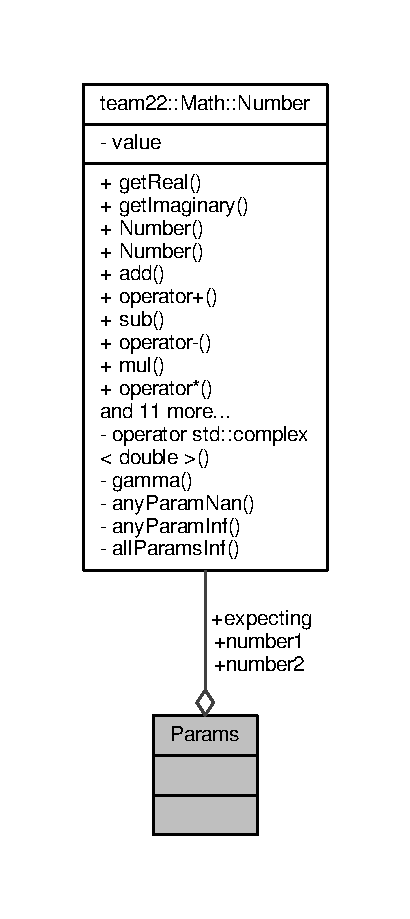
\includegraphics[width=197pt]{struct_params__coll__graph}
\end{center}
\end{figure}
\subsection*{Public Attributes}
\begin{DoxyCompactItemize}
\item 
\hyperlink{classteam22_1_1_math_1_1_number}{Number} \hyperlink{struct_params_abfbdd38f4448b9722ca7faeffdf4ef36}{number1}
\item 
\hyperlink{classteam22_1_1_math_1_1_number}{Number} \hyperlink{struct_params_af25f02c145e03d78112c0a3e7258155f}{number2}
\item 
\hyperlink{classteam22_1_1_math_1_1_number}{Number} \hyperlink{struct_params_ac15c821d1c46c6d5571f3ee32ba0fdbb}{expecting}
\end{DoxyCompactItemize}
\subsection*{Friends}
\begin{DoxyCompactItemize}
\item 
std\+::ostream \& \hyperlink{struct_params_ada7517152e144e49a36dd29a92ed8eb6}{operator$<$$<$} (std\+::ostream \&os, const \hyperlink{struct_params}{Params} \&params)
\end{DoxyCompactItemize}


\subsection{Detailed Description}


Definition at line 41 of file Number\+Test.\+cpp.



\subsection{Friends And Related Function Documentation}
\mbox{\Hypertarget{struct_params_ada7517152e144e49a36dd29a92ed8eb6}\label{struct_params_ada7517152e144e49a36dd29a92ed8eb6}} 
\index{Params@{Params}!operator$<$$<$@{operator$<$$<$}}
\index{operator$<$$<$@{operator$<$$<$}!Params@{Params}}
\subsubsection{\texorpdfstring{operator$<$$<$}{operator<<}}
{\footnotesize\ttfamily std\+::ostream\& operator$<$$<$ (\begin{DoxyParamCaption}\item[{std\+::ostream \&}]{os,  }\item[{const \hyperlink{struct_params}{Params} \&}]{params }\end{DoxyParamCaption})\hspace{0.3cm}{\ttfamily [friend]}}



Definition at line 46 of file Number\+Test.\+cpp.



\subsection{Member Data Documentation}
\mbox{\Hypertarget{struct_params_ac15c821d1c46c6d5571f3ee32ba0fdbb}\label{struct_params_ac15c821d1c46c6d5571f3ee32ba0fdbb}} 
\index{Params@{Params}!expecting@{expecting}}
\index{expecting@{expecting}!Params@{Params}}
\subsubsection{\texorpdfstring{expecting}{expecting}}
{\footnotesize\ttfamily \hyperlink{classteam22_1_1_math_1_1_number}{Number} Params\+::expecting}



Definition at line 44 of file Number\+Test.\+cpp.

\mbox{\Hypertarget{struct_params_abfbdd38f4448b9722ca7faeffdf4ef36}\label{struct_params_abfbdd38f4448b9722ca7faeffdf4ef36}} 
\index{Params@{Params}!number1@{number1}}
\index{number1@{number1}!Params@{Params}}
\subsubsection{\texorpdfstring{number1}{number1}}
{\footnotesize\ttfamily \hyperlink{classteam22_1_1_math_1_1_number}{Number} Params\+::number1}



Definition at line 42 of file Number\+Test.\+cpp.

\mbox{\Hypertarget{struct_params_af25f02c145e03d78112c0a3e7258155f}\label{struct_params_af25f02c145e03d78112c0a3e7258155f}} 
\index{Params@{Params}!number2@{number2}}
\index{number2@{number2}!Params@{Params}}
\subsubsection{\texorpdfstring{number2}{number2}}
{\footnotesize\ttfamily \hyperlink{classteam22_1_1_math_1_1_number}{Number} Params\+::number2}



Definition at line 43 of file Number\+Test.\+cpp.



The documentation for this struct was generated from the following file\+:\begin{DoxyCompactItemize}
\item 
src/tests/\hyperlink{_number_test_8cpp}{Number\+Test.\+cpp}\end{DoxyCompactItemize}

\hypertarget{struct_param_test}{}\section{Param\+Test Struct Reference}
\label{struct_param_test}\index{Param\+Test@{Param\+Test}}


Inheritance diagram for Param\+Test\+:
\nopagebreak
\begin{figure}[H]
\begin{center}
\leavevmode
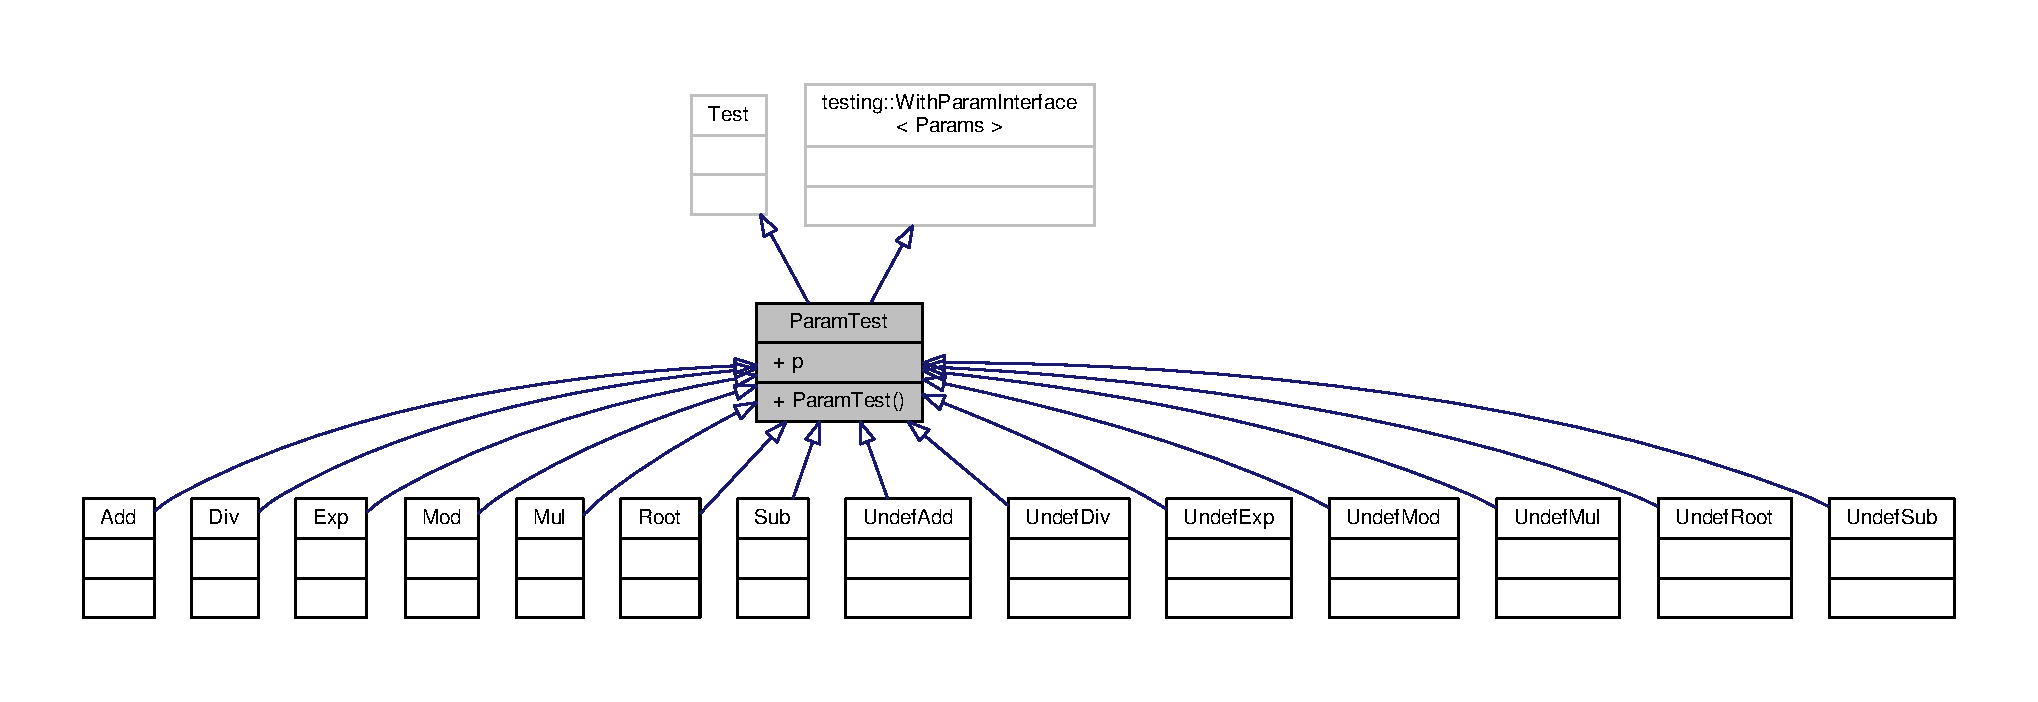
\includegraphics[width=350pt]{struct_param_test__inherit__graph}
\end{center}
\end{figure}


Collaboration diagram for Param\+Test\+:
\nopagebreak
\begin{figure}[H]
\begin{center}
\leavevmode
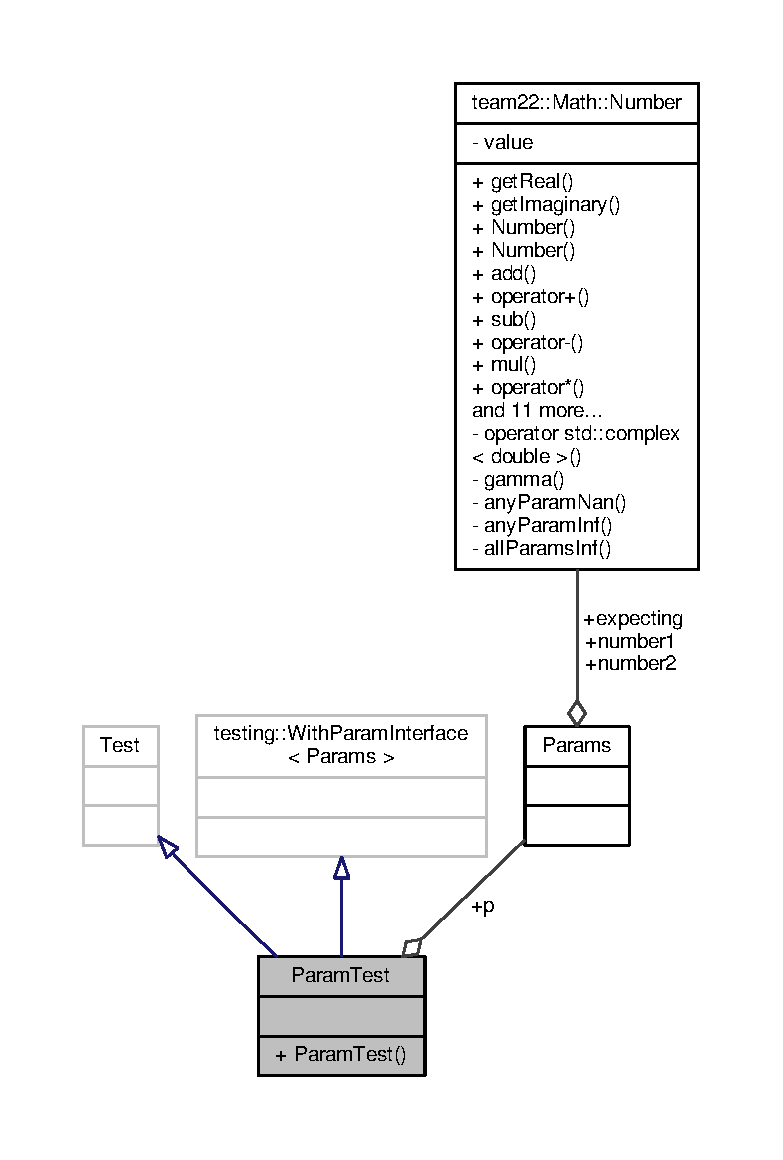
\includegraphics[width=350pt]{struct_param_test__coll__graph}
\end{center}
\end{figure}
\subsection*{Public Member Functions}
\begin{DoxyCompactItemize}
\item 
\hyperlink{struct_param_test_afd4f321e586d9c5e11f17f2c768d4067}{Param\+Test} ()
\end{DoxyCompactItemize}
\subsection*{Public Attributes}
\begin{DoxyCompactItemize}
\item 
\hyperlink{struct_params}{Params} \hyperlink{struct_param_test_ab4d405550f168d7a7e59abb75c315e50}{p} \{0,0,0\}
\end{DoxyCompactItemize}


\subsection{Detailed Description}


Definition at line 62 of file Number\+Test.\+cpp.



\subsection{Constructor \& Destructor Documentation}
\mbox{\Hypertarget{struct_param_test_afd4f321e586d9c5e11f17f2c768d4067}\label{struct_param_test_afd4f321e586d9c5e11f17f2c768d4067}} 
\index{Param\+Test@{Param\+Test}!Param\+Test@{Param\+Test}}
\index{Param\+Test@{Param\+Test}!Param\+Test@{Param\+Test}}
\subsubsection{\texorpdfstring{Param\+Test()}{ParamTest()}}
{\footnotesize\ttfamily Param\+Test\+::\+Param\+Test (\begin{DoxyParamCaption}{ }\end{DoxyParamCaption})\hspace{0.3cm}{\ttfamily [inline]}}



Definition at line 64 of file Number\+Test.\+cpp.



\subsection{Member Data Documentation}
\mbox{\Hypertarget{struct_param_test_ab4d405550f168d7a7e59abb75c315e50}\label{struct_param_test_ab4d405550f168d7a7e59abb75c315e50}} 
\index{Param\+Test@{Param\+Test}!p@{p}}
\index{p@{p}!Param\+Test@{Param\+Test}}
\subsubsection{\texorpdfstring{p}{p}}
{\footnotesize\ttfamily \hyperlink{struct_params}{Params} Param\+Test\+::p \{0,0,0\}}



Definition at line 63 of file Number\+Test.\+cpp.



The documentation for this struct was generated from the following file\+:\begin{DoxyCompactItemize}
\item 
src/tests/\hyperlink{_number_test_8cpp}{Number\+Test.\+cpp}\end{DoxyCompactItemize}

\hypertarget{classteam22_1_1_calc_1_1_result_observer}{}\section{team22\+:\+:Calc\+:\+:Result\+Observer Class Reference}
\label{classteam22_1_1_calc_1_1_result_observer}\index{team22\+::\+Calc\+::\+Result\+Observer@{team22\+::\+Calc\+::\+Result\+Observer}}


{\ttfamily \#include $<$Result\+Observer.\+h$>$}



Inheritance diagram for team22\+:\+:Calc\+:\+:Result\+Observer\+:
\nopagebreak
\begin{figure}[H]
\begin{center}
\leavevmode
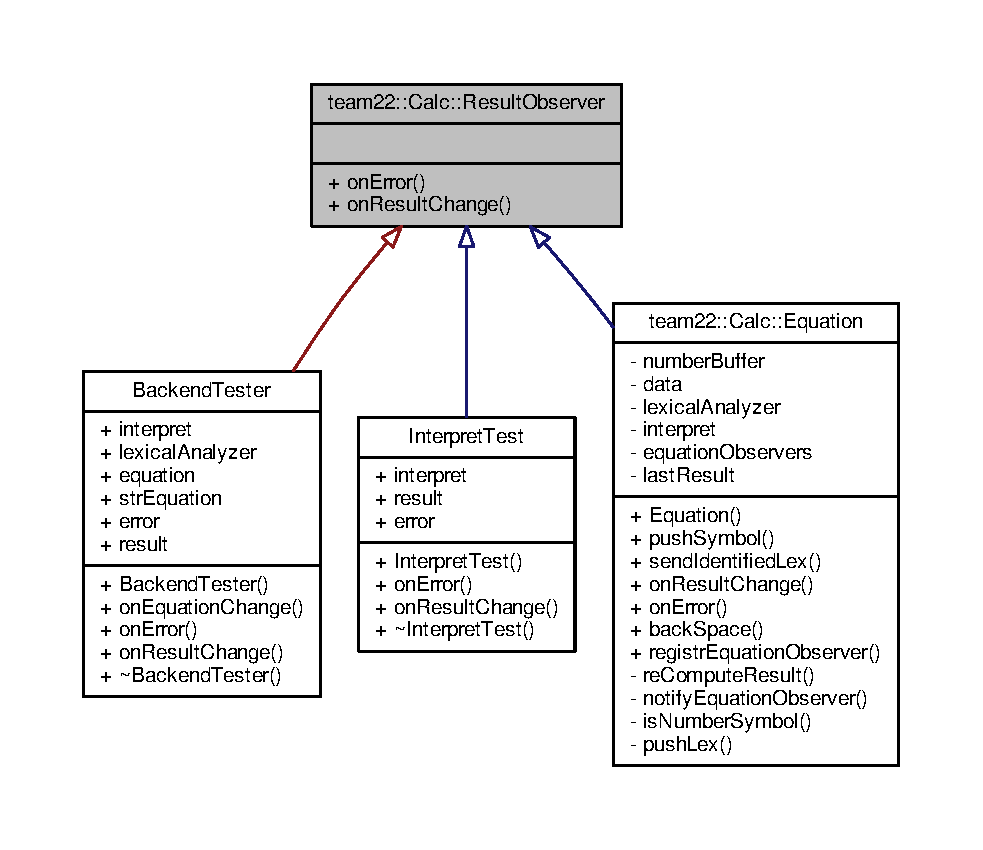
\includegraphics[width=229pt]{classteam22_1_1_calc_1_1_result_observer__inherit__graph}
\end{center}
\end{figure}


Collaboration diagram for team22\+:\+:Calc\+:\+:Result\+Observer\+:
\nopagebreak
\begin{figure}[H]
\begin{center}
\leavevmode
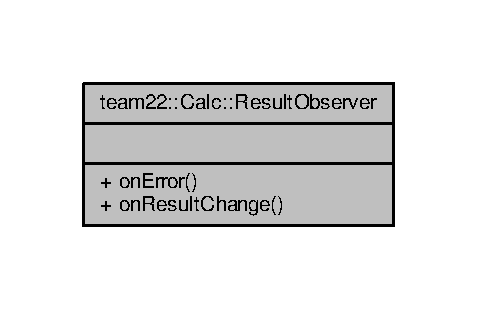
\includegraphics[width=229pt]{classteam22_1_1_calc_1_1_result_observer__coll__graph}
\end{center}
\end{figure}
\subsection*{Public Member Functions}
\begin{DoxyCompactItemize}
\item 
virtual void \hyperlink{classteam22_1_1_calc_1_1_result_observer_ad36cf8df89853d60f91094800c01d329}{on\+Error} (\hyperlink{class_interpret_exception}{Interpret\+Exception} exception)=0
\item 
virtual void \hyperlink{classteam22_1_1_calc_1_1_result_observer_aa04007df3aa8a499c3a511f549238285}{on\+Result\+Change} (Math\+::\+Number result)=0
\end{DoxyCompactItemize}


\subsection{Detailed Description}


Definition at line 15 of file Result\+Observer.\+h.



\subsection{Member Function Documentation}
\mbox{\Hypertarget{classteam22_1_1_calc_1_1_result_observer_ad36cf8df89853d60f91094800c01d329}\label{classteam22_1_1_calc_1_1_result_observer_ad36cf8df89853d60f91094800c01d329}} 
\index{team22\+::\+Calc\+::\+Result\+Observer@{team22\+::\+Calc\+::\+Result\+Observer}!on\+Error@{on\+Error}}
\index{on\+Error@{on\+Error}!team22\+::\+Calc\+::\+Result\+Observer@{team22\+::\+Calc\+::\+Result\+Observer}}
\subsubsection{\texorpdfstring{on\+Error()}{onError()}}
{\footnotesize\ttfamily virtual void team22\+::\+Calc\+::\+Result\+Observer\+::on\+Error (\begin{DoxyParamCaption}\item[{\hyperlink{class_interpret_exception}{Interpret\+Exception}}]{exception }\end{DoxyParamCaption})\hspace{0.3cm}{\ttfamily [pure virtual]}}

Callback volaný pokud vznikla chyba při výpočtu 
\begin{DoxyParams}{Parameters}
{\em \hyperlink{class_interpret_exception}{Interpret\+Exception}} & \\
\hline
\end{DoxyParams}


Implemented in \hyperlink{classteam22_1_1_calc_1_1_equation_a4e7a0614867931bcc714440441cdd894}{team22\+::\+Calc\+::\+Equation}.

\mbox{\Hypertarget{classteam22_1_1_calc_1_1_result_observer_aa04007df3aa8a499c3a511f549238285}\label{classteam22_1_1_calc_1_1_result_observer_aa04007df3aa8a499c3a511f549238285}} 
\index{team22\+::\+Calc\+::\+Result\+Observer@{team22\+::\+Calc\+::\+Result\+Observer}!on\+Result\+Change@{on\+Result\+Change}}
\index{on\+Result\+Change@{on\+Result\+Change}!team22\+::\+Calc\+::\+Result\+Observer@{team22\+::\+Calc\+::\+Result\+Observer}}
\subsubsection{\texorpdfstring{on\+Result\+Change()}{onResultChange()}}
{\footnotesize\ttfamily virtual void team22\+::\+Calc\+::\+Result\+Observer\+::on\+Result\+Change (\begin{DoxyParamCaption}\item[{Math\+::\+Number}]{result }\end{DoxyParamCaption})\hspace{0.3cm}{\ttfamily [pure virtual]}}

Callback volaný při změně výsledku 
\begin{DoxyParams}{Parameters}
{\em result} & \\
\hline
\end{DoxyParams}


Implemented in \hyperlink{classteam22_1_1_calc_1_1_equation_a302c295e099f589897a1bad4b02d3de8}{team22\+::\+Calc\+::\+Equation}.



The documentation for this class was generated from the following file\+:\begin{DoxyCompactItemize}
\item 
\hyperlink{_result_observer_8h}{Result\+Observer.\+h}\end{DoxyCompactItemize}

\hypertarget{struct_root}{}\section{Root Struct Reference}
\label{struct_root}\index{Root@{Root}}


Inheritance diagram for Root\+:
\nopagebreak
\begin{figure}[H]
\begin{center}
\leavevmode
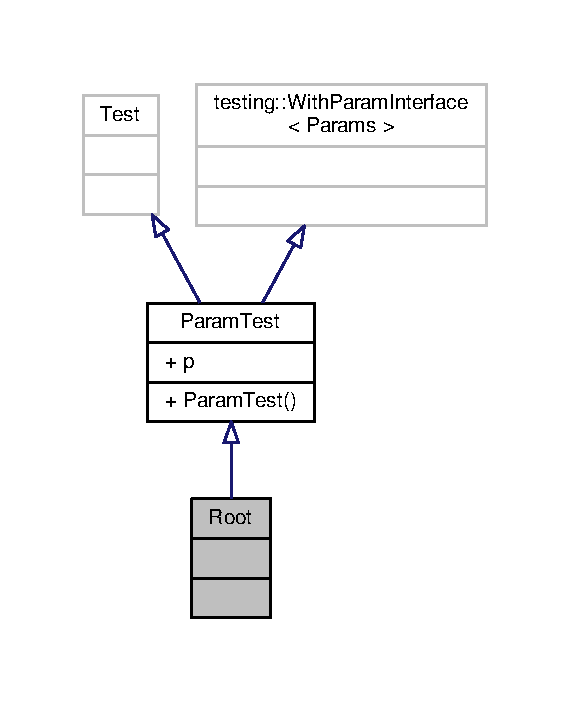
\includegraphics[width=274pt]{struct_root__inherit__graph}
\end{center}
\end{figure}


Collaboration diagram for Root\+:
\nopagebreak
\begin{figure}[H]
\begin{center}
\leavevmode
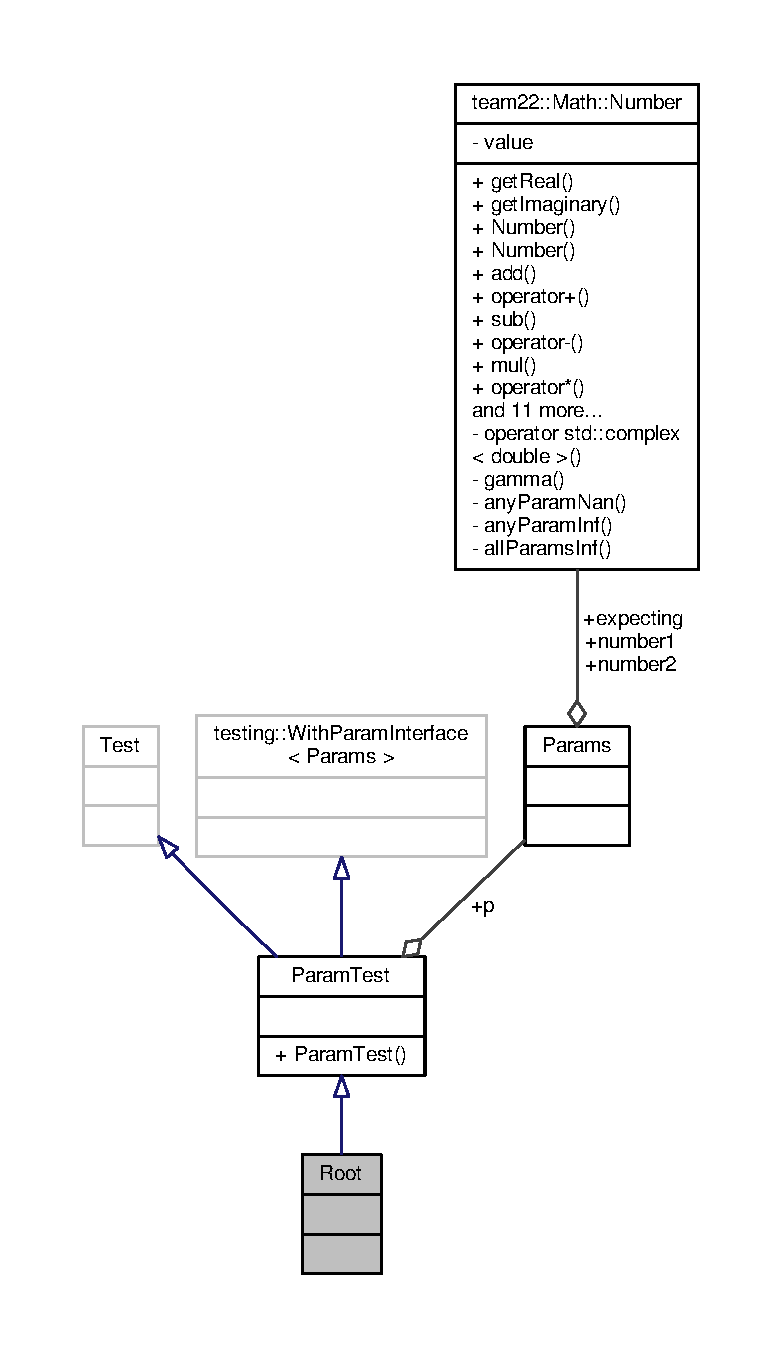
\includegraphics[height=550pt]{struct_root__coll__graph}
\end{center}
\end{figure}
\subsection*{Additional Inherited Members}


\subsection{Detailed Description}


Definition at line 78 of file Number\+Test.\+cpp.



The documentation for this struct was generated from the following file\+:\begin{DoxyCompactItemize}
\item 
src/tests/\hyperlink{_number_test_8cpp}{Number\+Test.\+cpp}\end{DoxyCompactItemize}

\hypertarget{struct_sub}{}\section{Sub Struct Reference}
\label{struct_sub}\index{Sub@{Sub}}


Inheritance diagram for Sub\+:
\nopagebreak
\begin{figure}[H]
\begin{center}
\leavevmode
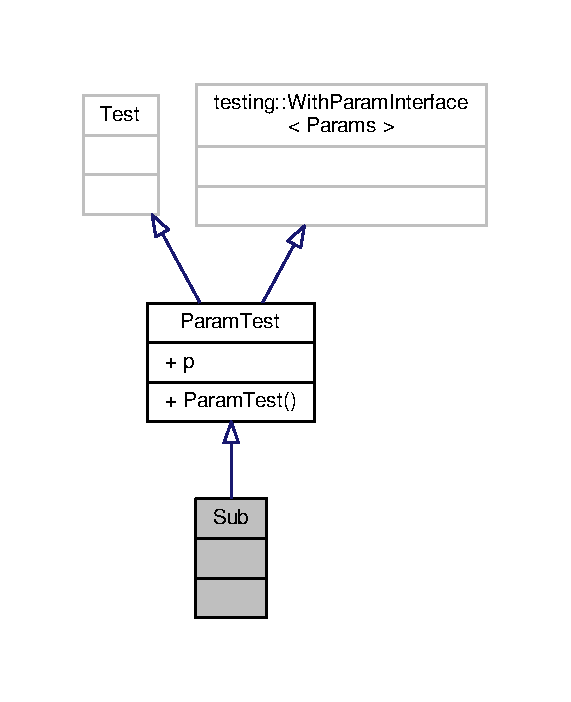
\includegraphics[width=274pt]{struct_sub__inherit__graph}
\end{center}
\end{figure}


Collaboration diagram for Sub\+:
\nopagebreak
\begin{figure}[H]
\begin{center}
\leavevmode
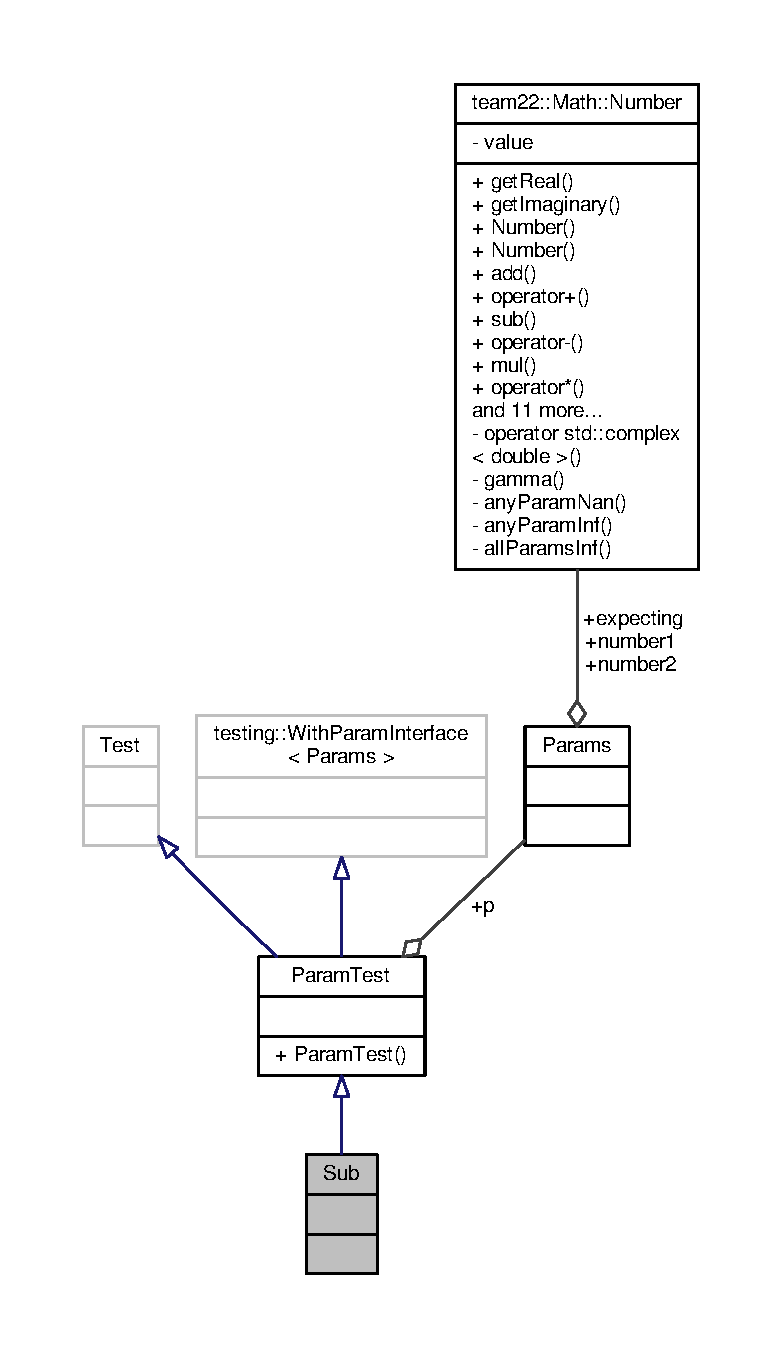
\includegraphics[height=550pt]{struct_sub__coll__graph}
\end{center}
\end{figure}
\subsection*{Additional Inherited Members}


\subsection{Detailed Description}


Definition at line 73 of file Number\+Test.\+cpp.



The documentation for this struct was generated from the following file\+:\begin{DoxyCompactItemize}
\item 
src/tests/\hyperlink{_number_test_8cpp}{Number\+Test.\+cpp}\end{DoxyCompactItemize}

\hypertarget{struct_unari_params}{}\section{Unari\+Params Struct Reference}
\label{struct_unari_params}\index{Unari\+Params@{Unari\+Params}}


Collaboration diagram for Unari\+Params\+:
\nopagebreak
\begin{figure}[H]
\begin{center}
\leavevmode
\includegraphics[width=197pt]{struct_unari_params__coll__graph}
\end{center}
\end{figure}
\subsection*{Public Attributes}
\begin{DoxyCompactItemize}
\item 
\hyperlink{classteam22_1_1_math_1_1_number}{Number} \hyperlink{struct_unari_params_a85762f9bb00163170524b43c7947dca1}{number}
\item 
\hyperlink{classteam22_1_1_math_1_1_number}{Number} \hyperlink{struct_unari_params_a4ea568291d8eb7ad9431e8457787d25f}{expecting}
\end{DoxyCompactItemize}
\subsection*{Friends}
\begin{DoxyCompactItemize}
\item 
std\+::ostream \& \hyperlink{struct_unari_params_a45b95d770513e8cfe4385f18085715df}{operator$<$$<$} (std\+::ostream \&os, const \hyperlink{struct_unari_params}{Unari\+Params} \&params)
\end{DoxyCompactItemize}


\subsection{Detailed Description}


Definition at line 53 of file Number\+Test.\+cpp.



\subsection{Friends And Related Function Documentation}
\mbox{\Hypertarget{struct_unari_params_a45b95d770513e8cfe4385f18085715df}\label{struct_unari_params_a45b95d770513e8cfe4385f18085715df}} 
\index{Unari\+Params@{Unari\+Params}!operator$<$$<$@{operator$<$$<$}}
\index{operator$<$$<$@{operator$<$$<$}!Unari\+Params@{Unari\+Params}}
\subsubsection{\texorpdfstring{operator$<$$<$}{operator<<}}
{\footnotesize\ttfamily std\+::ostream\& operator$<$$<$ (\begin{DoxyParamCaption}\item[{std\+::ostream \&}]{os,  }\item[{const \hyperlink{struct_unari_params}{Unari\+Params} \&}]{params }\end{DoxyParamCaption})\hspace{0.3cm}{\ttfamily [friend]}}



Definition at line 56 of file Number\+Test.\+cpp.



\subsection{Member Data Documentation}
\mbox{\Hypertarget{struct_unari_params_a4ea568291d8eb7ad9431e8457787d25f}\label{struct_unari_params_a4ea568291d8eb7ad9431e8457787d25f}} 
\index{Unari\+Params@{Unari\+Params}!expecting@{expecting}}
\index{expecting@{expecting}!Unari\+Params@{Unari\+Params}}
\subsubsection{\texorpdfstring{expecting}{expecting}}
{\footnotesize\ttfamily \hyperlink{classteam22_1_1_math_1_1_number}{Number} Unari\+Params\+::expecting}



Definition at line 55 of file Number\+Test.\+cpp.

\mbox{\Hypertarget{struct_unari_params_a85762f9bb00163170524b43c7947dca1}\label{struct_unari_params_a85762f9bb00163170524b43c7947dca1}} 
\index{Unari\+Params@{Unari\+Params}!number@{number}}
\index{number@{number}!Unari\+Params@{Unari\+Params}}
\subsubsection{\texorpdfstring{number}{number}}
{\footnotesize\ttfamily \hyperlink{classteam22_1_1_math_1_1_number}{Number} Unari\+Params\+::number}



Definition at line 54 of file Number\+Test.\+cpp.



The documentation for this struct was generated from the following file\+:\begin{DoxyCompactItemize}
\item 
tests/\hyperlink{_number_test_8cpp}{Number\+Test.\+cpp}\end{DoxyCompactItemize}

\hypertarget{struct_undef_add}{}\section{Undef\+Add Struct Reference}
\label{struct_undef_add}\index{Undef\+Add@{Undef\+Add}}


Inheritance diagram for Undef\+Add\+:
\nopagebreak
\begin{figure}[H]
\begin{center}
\leavevmode
\includegraphics[width=274pt]{struct_undef_add__inherit__graph}
\end{center}
\end{figure}


Collaboration diagram for Undef\+Add\+:
\nopagebreak
\begin{figure}[H]
\begin{center}
\leavevmode
\includegraphics[height=550pt]{struct_undef_add__coll__graph}
\end{center}
\end{figure}
\subsection*{Additional Inherited Members}


\subsection{Detailed Description}


Definition at line 484 of file Number\+Test.\+cpp.



The documentation for this struct was generated from the following file\+:\begin{DoxyCompactItemize}
\item 
src/tests/\hyperlink{_number_test_8cpp}{Number\+Test.\+cpp}\end{DoxyCompactItemize}

\hypertarget{struct_undef_div}{}\section{Undef\+Div Struct Reference}
\label{struct_undef_div}\index{Undef\+Div@{Undef\+Div}}


Inheritance diagram for Undef\+Div\+:
\nopagebreak
\begin{figure}[H]
\begin{center}
\leavevmode
\includegraphics[width=274pt]{struct_undef_div__inherit__graph}
\end{center}
\end{figure}


Collaboration diagram for Undef\+Div\+:
\nopagebreak
\begin{figure}[H]
\begin{center}
\leavevmode
\includegraphics[height=550pt]{struct_undef_div__coll__graph}
\end{center}
\end{figure}
\subsection*{Additional Inherited Members}


\subsection{Detailed Description}


Definition at line 486 of file Number\+Test.\+cpp.



The documentation for this struct was generated from the following file\+:\begin{DoxyCompactItemize}
\item 
tests/\hyperlink{_number_test_8cpp}{Number\+Test.\+cpp}\end{DoxyCompactItemize}

\hypertarget{struct_undef_exp}{}\section{Undef\+Exp Struct Reference}
\label{struct_undef_exp}\index{Undef\+Exp@{Undef\+Exp}}


Inheritance diagram for Undef\+Exp\+:
\nopagebreak
\begin{figure}[H]
\begin{center}
\leavevmode
\includegraphics[width=274pt]{struct_undef_exp__inherit__graph}
\end{center}
\end{figure}


Collaboration diagram for Undef\+Exp\+:
\nopagebreak
\begin{figure}[H]
\begin{center}
\leavevmode
\includegraphics[height=550pt]{struct_undef_exp__coll__graph}
\end{center}
\end{figure}
\subsection*{Additional Inherited Members}


\subsection{Detailed Description}


Definition at line 487 of file Number\+Test.\+cpp.



The documentation for this struct was generated from the following file\+:\begin{DoxyCompactItemize}
\item 
tests/\hyperlink{_number_test_8cpp}{Number\+Test.\+cpp}\end{DoxyCompactItemize}

\hypertarget{struct_undef_factorial}{}\section{Undef\+Factorial Struct Reference}
\label{struct_undef_factorial}\index{Undef\+Factorial@{Undef\+Factorial}}


Inheritance diagram for Undef\+Factorial\+:
\nopagebreak
\begin{figure}[H]
\begin{center}
\leavevmode
\includegraphics[width=274pt]{struct_undef_factorial__inherit__graph}
\end{center}
\end{figure}


Collaboration diagram for Undef\+Factorial\+:
\nopagebreak
\begin{figure}[H]
\begin{center}
\leavevmode
\includegraphics[height=550pt]{struct_undef_factorial__coll__graph}
\end{center}
\end{figure}
\subsection*{Additional Inherited Members}


\subsection{Detailed Description}


Definition at line 490 of file Number\+Test.\+cpp.



The documentation for this struct was generated from the following file\+:\begin{DoxyCompactItemize}
\item 
tests/\hyperlink{_number_test_8cpp}{Number\+Test.\+cpp}\end{DoxyCompactItemize}

\hypertarget{classteam22_1_1_math_1_1_undefined_exception}{}\section{team22\+:\+:Math\+:\+:Undefined\+Exception Class Reference}
\label{classteam22_1_1_math_1_1_undefined_exception}\index{team22\+::\+Math\+::\+Undefined\+Exception@{team22\+::\+Math\+::\+Undefined\+Exception}}


{\ttfamily \#include $<$Undefined\+Exception.\+h$>$}



Inheritance diagram for team22\+:\+:Math\+:\+:Undefined\+Exception\+:
\nopagebreak
\begin{figure}[H]
\begin{center}
\leavevmode
\includegraphics[width=250pt]{classteam22_1_1_math_1_1_undefined_exception__inherit__graph}
\end{center}
\end{figure}


Collaboration diagram for team22\+:\+:Math\+:\+:Undefined\+Exception\+:
\nopagebreak
\begin{figure}[H]
\begin{center}
\leavevmode
\includegraphics[width=250pt]{classteam22_1_1_math_1_1_undefined_exception__coll__graph}
\end{center}
\end{figure}
\subsection*{Public Member Functions}
\begin{DoxyCompactItemize}
\item 
const char $\ast$ \hyperlink{classteam22_1_1_math_1_1_undefined_exception_a568d4e05844e57b984c3b37e3956d334}{what} ()
\end{DoxyCompactItemize}


\subsection{Detailed Description}
Výjimka vrácena pokud operace pro vstupy mimo definiční obor fce 

Definition at line 17 of file Undefined\+Exception.\+h.



\subsection{Member Function Documentation}
\mbox{\Hypertarget{classteam22_1_1_math_1_1_undefined_exception_a568d4e05844e57b984c3b37e3956d334}\label{classteam22_1_1_math_1_1_undefined_exception_a568d4e05844e57b984c3b37e3956d334}} 
\index{team22\+::\+Math\+::\+Undefined\+Exception@{team22\+::\+Math\+::\+Undefined\+Exception}!what@{what}}
\index{what@{what}!team22\+::\+Math\+::\+Undefined\+Exception@{team22\+::\+Math\+::\+Undefined\+Exception}}
\subsubsection{\texorpdfstring{what()}{what()}}
{\footnotesize\ttfamily const char$\ast$ team22\+::\+Math\+::\+Undefined\+Exception\+::what (\begin{DoxyParamCaption}{ }\end{DoxyParamCaption})\hspace{0.3cm}{\ttfamily [inline]}}



Definition at line 21 of file Undefined\+Exception.\+h.



The documentation for this class was generated from the following file\+:\begin{DoxyCompactItemize}
\item 
math/\hyperlink{_undefined_exception_8h}{Undefined\+Exception.\+h}\end{DoxyCompactItemize}

\hypertarget{struct_undef_mod}{}\section{Undef\+Mod Struct Reference}
\label{struct_undef_mod}\index{Undef\+Mod@{Undef\+Mod}}


Inheritance diagram for Undef\+Mod\+:
\nopagebreak
\begin{figure}[H]
\begin{center}
\leavevmode
\includegraphics[width=274pt]{struct_undef_mod__inherit__graph}
\end{center}
\end{figure}


Collaboration diagram for Undef\+Mod\+:
\nopagebreak
\begin{figure}[H]
\begin{center}
\leavevmode
\includegraphics[height=550pt]{struct_undef_mod__coll__graph}
\end{center}
\end{figure}
\subsection*{Additional Inherited Members}


\subsection{Detailed Description}


Definition at line 489 of file Number\+Test.\+cpp.



The documentation for this struct was generated from the following file\+:\begin{DoxyCompactItemize}
\item 
src/tests/\hyperlink{_number_test_8cpp}{Number\+Test.\+cpp}\end{DoxyCompactItemize}

\hypertarget{struct_undef_mul}{}\section{Undef\+Mul Struct Reference}
\label{struct_undef_mul}\index{Undef\+Mul@{Undef\+Mul}}


Inheritance diagram for Undef\+Mul\+:
\nopagebreak
\begin{figure}[H]
\begin{center}
\leavevmode
\includegraphics[width=274pt]{struct_undef_mul__inherit__graph}
\end{center}
\end{figure}


Collaboration diagram for Undef\+Mul\+:
\nopagebreak
\begin{figure}[H]
\begin{center}
\leavevmode
\includegraphics[height=550pt]{struct_undef_mul__coll__graph}
\end{center}
\end{figure}
\subsection*{Additional Inherited Members}


\subsection{Detailed Description}


Definition at line 485 of file Number\+Test.\+cpp.



The documentation for this struct was generated from the following file\+:\begin{DoxyCompactItemize}
\item 
tests/\hyperlink{_number_test_8cpp}{Number\+Test.\+cpp}\end{DoxyCompactItemize}

\hypertarget{struct_undef_root}{}\section{Undef\+Root Struct Reference}
\label{struct_undef_root}\index{Undef\+Root@{Undef\+Root}}


Inheritance diagram for Undef\+Root\+:
\nopagebreak
\begin{figure}[H]
\begin{center}
\leavevmode
\includegraphics[width=274pt]{struct_undef_root__inherit__graph}
\end{center}
\end{figure}


Collaboration diagram for Undef\+Root\+:
\nopagebreak
\begin{figure}[H]
\begin{center}
\leavevmode
\includegraphics[height=550pt]{struct_undef_root__coll__graph}
\end{center}
\end{figure}
\subsection*{Additional Inherited Members}


\subsection{Detailed Description}


Definition at line 488 of file Number\+Test.\+cpp.



The documentation for this struct was generated from the following file\+:\begin{DoxyCompactItemize}
\item 
src/tests/\hyperlink{_number_test_8cpp}{Number\+Test.\+cpp}\end{DoxyCompactItemize}

\hypertarget{struct_undef_sub}{}\section{Undef\+Sub Struct Reference}
\label{struct_undef_sub}\index{Undef\+Sub@{Undef\+Sub}}


Inheritance diagram for Undef\+Sub\+:
\nopagebreak
\begin{figure}[H]
\begin{center}
\leavevmode
\includegraphics[width=274pt]{struct_undef_sub__inherit__graph}
\end{center}
\end{figure}


Collaboration diagram for Undef\+Sub\+:
\nopagebreak
\begin{figure}[H]
\begin{center}
\leavevmode
\includegraphics[height=550pt]{struct_undef_sub__coll__graph}
\end{center}
\end{figure}
\subsection*{Additional Inherited Members}


\subsection{Detailed Description}


Definition at line 483 of file Number\+Test.\+cpp.



The documentation for this struct was generated from the following file\+:\begin{DoxyCompactItemize}
\item 
src/tests/\hyperlink{_number_test_8cpp}{Number\+Test.\+cpp}\end{DoxyCompactItemize}

\hypertarget{struct_u_param_test}{}\section{U\+Param\+Test Struct Reference}
\label{struct_u_param_test}\index{U\+Param\+Test@{U\+Param\+Test}}


Inheritance diagram for U\+Param\+Test\+:
\nopagebreak
\begin{figure}[H]
\begin{center}
\leavevmode
\includegraphics[width=274pt]{struct_u_param_test__inherit__graph}
\end{center}
\end{figure}


Collaboration diagram for U\+Param\+Test\+:
\nopagebreak
\begin{figure}[H]
\begin{center}
\leavevmode
\includegraphics[width=350pt]{struct_u_param_test__coll__graph}
\end{center}
\end{figure}
\subsection*{Public Member Functions}
\begin{DoxyCompactItemize}
\item 
\hyperlink{struct_u_param_test_a4460d7e228030b3a5b6bd35cd59656be}{U\+Param\+Test} ()
\end{DoxyCompactItemize}
\subsection*{Public Attributes}
\begin{DoxyCompactItemize}
\item 
\hyperlink{struct_unari_params}{Unari\+Params} \hyperlink{struct_u_param_test_ab8f85343a35eded9f31b05a7869608c9}{p} \{0,0\}
\end{DoxyCompactItemize}


\subsection{Detailed Description}


Definition at line 68 of file Number\+Test.\+cpp.



\subsection{Constructor \& Destructor Documentation}
\mbox{\Hypertarget{struct_u_param_test_a4460d7e228030b3a5b6bd35cd59656be}\label{struct_u_param_test_a4460d7e228030b3a5b6bd35cd59656be}} 
\index{U\+Param\+Test@{U\+Param\+Test}!U\+Param\+Test@{U\+Param\+Test}}
\index{U\+Param\+Test@{U\+Param\+Test}!U\+Param\+Test@{U\+Param\+Test}}
\subsubsection{\texorpdfstring{U\+Param\+Test()}{UParamTest()}}
{\footnotesize\ttfamily U\+Param\+Test\+::\+U\+Param\+Test (\begin{DoxyParamCaption}{ }\end{DoxyParamCaption})\hspace{0.3cm}{\ttfamily [inline]}}



Definition at line 70 of file Number\+Test.\+cpp.



\subsection{Member Data Documentation}
\mbox{\Hypertarget{struct_u_param_test_ab8f85343a35eded9f31b05a7869608c9}\label{struct_u_param_test_ab8f85343a35eded9f31b05a7869608c9}} 
\index{U\+Param\+Test@{U\+Param\+Test}!p@{p}}
\index{p@{p}!U\+Param\+Test@{U\+Param\+Test}}
\subsubsection{\texorpdfstring{p}{p}}
{\footnotesize\ttfamily \hyperlink{struct_unari_params}{Unari\+Params} U\+Param\+Test\+::p \{0,0\}}



Definition at line 69 of file Number\+Test.\+cpp.



The documentation for this struct was generated from the following file\+:\begin{DoxyCompactItemize}
\item 
tests/\hyperlink{_number_test_8cpp}{Number\+Test.\+cpp}\end{DoxyCompactItemize}

\hypertarget{unionteam22_1_1_calc_1_1_lex_1_1_value}{}\section{team22\+:\+:Calc\+:\+:Lex\+:\+:Value Union Reference}
\label{unionteam22_1_1_calc_1_1_lex_1_1_value}\index{team22\+::\+Calc\+::\+Lex\+::\+Value@{team22\+::\+Calc\+::\+Lex\+::\+Value}}


reprezentace hodnoty lexému  




{\ttfamily \#include $<$Lex.\+h$>$}



Collaboration diagram for team22\+:\+:Calc\+:\+:Lex\+:\+:Value\+:
\nopagebreak
\begin{figure}[H]
\begin{center}
\leavevmode
\includegraphics[width=197pt]{unionteam22_1_1_calc_1_1_lex_1_1_value__coll__graph}
\end{center}
\end{figure}
\subsection*{Public Attributes}
\begin{DoxyCompactItemize}
\item 
\hyperlink{classteam22_1_1_math_1_1_number}{Math\+::\+Number} \hyperlink{unionteam22_1_1_calc_1_1_lex_1_1_value_a86e2e3ea0c887ca50885bcdb8f1ec5ce}{number} \{0\}
\item 
\hyperlink{classteam22_1_1_calc_1_1_lex_a61d29fc4878a3b36d2de2f13c56ed932}{Operator} \hyperlink{unionteam22_1_1_calc_1_1_lex_1_1_value_ade46fa860d495ce4d431d3934210579d}{oper}
\end{DoxyCompactItemize}


\subsection{Detailed Description}
reprezentace hodnoty lexému 

Definition at line 67 of file Lex.\+h.



\subsection{Member Data Documentation}
\mbox{\Hypertarget{unionteam22_1_1_calc_1_1_lex_1_1_value_a86e2e3ea0c887ca50885bcdb8f1ec5ce}\label{unionteam22_1_1_calc_1_1_lex_1_1_value_a86e2e3ea0c887ca50885bcdb8f1ec5ce}} 
\index{team22\+::\+Calc\+::\+Lex\+::\+Value@{team22\+::\+Calc\+::\+Lex\+::\+Value}!number@{number}}
\index{number@{number}!team22\+::\+Calc\+::\+Lex\+::\+Value@{team22\+::\+Calc\+::\+Lex\+::\+Value}}
\subsubsection{\texorpdfstring{number}{number}}
{\footnotesize\ttfamily \hyperlink{classteam22_1_1_math_1_1_number}{Math\+::\+Number} team22\+::\+Calc\+::\+Lex\+::\+Value\+::number \{0\}}



Definition at line 69 of file Lex.\+h.



Referenced by team22\+::\+Calc\+::\+Lex\+::get\+As\+Number(), and team22\+::\+Calc\+::\+Lex\+::\+Lex().

\mbox{\Hypertarget{unionteam22_1_1_calc_1_1_lex_1_1_value_ade46fa860d495ce4d431d3934210579d}\label{unionteam22_1_1_calc_1_1_lex_1_1_value_ade46fa860d495ce4d431d3934210579d}} 
\index{team22\+::\+Calc\+::\+Lex\+::\+Value@{team22\+::\+Calc\+::\+Lex\+::\+Value}!oper@{oper}}
\index{oper@{oper}!team22\+::\+Calc\+::\+Lex\+::\+Value@{team22\+::\+Calc\+::\+Lex\+::\+Value}}
\subsubsection{\texorpdfstring{oper}{oper}}
{\footnotesize\ttfamily \hyperlink{classteam22_1_1_calc_1_1_lex_a61d29fc4878a3b36d2de2f13c56ed932}{Operator} team22\+::\+Calc\+::\+Lex\+::\+Value\+::oper}



Definition at line 70 of file Lex.\+h.



Referenced by team22\+::\+Calc\+::\+Lex\+::get\+As\+Operator(), and team22\+::\+Calc\+::\+Lex\+::\+Lex().



The documentation for this union was generated from the following file\+:\begin{DoxyCompactItemize}
\item 
\hyperlink{_lex_8h}{Lex.\+h}\end{DoxyCompactItemize}

\chapter{File Documentation}
\hypertarget{xcecha04__xmatla00__xmitur01__xslade21__plan_8md}{}\section{plan/xcecha04\+\_\+xmatla00\+\_\+xmitur01\+\_\+xslade21\+\_\+plan.md File Reference}
\label{xcecha04__xmatla00__xmitur01__xslade21__plan_8md}\index{plan/xcecha04\+\_\+xmatla00\+\_\+xmitur01\+\_\+xslade21\+\_\+plan.\+md@{plan/xcecha04\+\_\+xmatla00\+\_\+xmitur01\+\_\+xslade21\+\_\+plan.\+md}}

\hypertarget{_r_e_a_d_m_e_8md}{}\section{R\+E\+A\+D\+M\+E.\+md File Reference}
\label{_r_e_a_d_m_e_8md}\index{R\+E\+A\+D\+M\+E.\+md@{R\+E\+A\+D\+M\+E.\+md}}

\hypertarget{_equation_8cpp}{}\section{src/\+Equation.cpp File Reference}
\label{_equation_8cpp}\index{src/\+Equation.\+cpp@{src/\+Equation.\+cpp}}
{\ttfamily \#include \char`\"{}Equation.\+h\char`\"{}}\newline
Include dependency graph for Equation.\+cpp\+:
\nopagebreak
\begin{figure}[H]
\begin{center}
\leavevmode
\includegraphics[width=350pt]{_equation_8cpp__incl}
\end{center}
\end{figure}


\subsection{Detailed Description}
U\+T\+F-\/8 \begin{DoxyDate}{Date}
8.\+4.\+18 
\end{DoxyDate}
\begin{DoxyAuthor}{Author}
Adam Mátl \href{mailto:xmatla00@stud.fit.vutbr.cz}{\tt xmatla00@stud.\+fit.\+vutbr.\+cz} \href{mailto:matla@matla.cz}{\tt matla@matla.\+cz} 
\end{DoxyAuthor}

\hypertarget{_equation_8h}{}\section{src/\+Equation.h File Reference}
\label{_equation_8h}\index{src/\+Equation.\+h@{src/\+Equation.\+h}}
{\ttfamily \#include \char`\"{}Lex\+Identification\+Observer.\+h\char`\"{}}\newline
{\ttfamily \#include \char`\"{}Lexical\+Analyzer.\+h\char`\"{}}\newline
{\ttfamily \#include \char`\"{}Equation\+Observer.\+h\char`\"{}}\newline
{\ttfamily \#include $<$string$>$}\newline
{\ttfamily \#include $<$vector$>$}\newline
{\ttfamily \#include $<$sstream$>$}\newline
{\ttfamily \#include $<$ostream$>$}\newline
Include dependency graph for Equation.\+h\+:
\nopagebreak
\begin{figure}[H]
\begin{center}
\leavevmode
\includegraphics[width=350pt]{_equation_8h__incl}
\end{center}
\end{figure}
This graph shows which files directly or indirectly include this file\+:
\nopagebreak
\begin{figure}[H]
\begin{center}
\leavevmode
\includegraphics[width=322pt]{_equation_8h__dep__incl}
\end{center}
\end{figure}
\subsection*{Classes}
\begin{DoxyCompactItemize}
\item 
class \hyperlink{classteam22_1_1_calc_1_1_equation}{team22\+::\+Calc\+::\+Equation}
\begin{DoxyCompactList}\small\item\em Třída reprezentující rovnici. \end{DoxyCompactList}\end{DoxyCompactItemize}
\subsection*{Namespaces}
\begin{DoxyCompactItemize}
\item 
 \hyperlink{namespaceteam22_1_1_calc}{team22\+::\+Calc}
\end{DoxyCompactItemize}


\subsection{Detailed Description}
U\+T\+F-\/8 \begin{DoxyDate}{Date}
8.\+4.\+18 
\end{DoxyDate}
\begin{DoxyAuthor}{Author}
Adam Mátl \href{mailto:xmatla00@stud.fit.vutbr.cz}{\tt xmatla00@stud.\+fit.\+vutbr.\+cz} \href{mailto:matla@matla.cz}{\tt matla@matla.\+cz} 
\end{DoxyAuthor}

\hypertarget{_equation_observer_8h}{}\section{Equation\+Observer.\+h File Reference}
\label{_equation_observer_8h}\index{Equation\+Observer.\+h@{Equation\+Observer.\+h}}
This graph shows which files directly or indirectly include this file\+:
\nopagebreak
\begin{figure}[H]
\begin{center}
\leavevmode
\includegraphics[width=183pt]{_equation_observer_8h__dep__incl}
\end{center}
\end{figure}
\subsection*{Classes}
\begin{DoxyCompactItemize}
\item 
class \hyperlink{classteam22_1_1_calc_1_1_equation_observer}{team22\+::\+Calc\+::\+Equation\+Observer}
\end{DoxyCompactItemize}
\subsection*{Namespaces}
\begin{DoxyCompactItemize}
\item 
 \hyperlink{namespaceteam22_1_1_calc}{team22\+::\+Calc}
\end{DoxyCompactItemize}


\subsection{Detailed Description}
U\+T\+F-\/8 \begin{DoxyDate}{Date}
8.\+4.\+18 
\end{DoxyDate}
\begin{DoxyAuthor}{Author}
Adam Mátl \href{mailto:xmatla00@stud.fit.vutbr.cz}{\tt xmatla00@stud.\+fit.\+vutbr.\+cz} \href{mailto:matla@matla.cz}{\tt matla@matla.\+cz} 
\end{DoxyAuthor}

\hypertarget{_interpret_8cpp}{}\section{src/\+Interpret.cpp File Reference}
\label{_interpret_8cpp}\index{src/\+Interpret.\+cpp@{src/\+Interpret.\+cpp}}
{\ttfamily \#include \char`\"{}Interpret.\+h\char`\"{}}\newline
Include dependency graph for Interpret.\+cpp\+:
\nopagebreak
\begin{figure}[H]
\begin{center}
\leavevmode
\includegraphics[width=350pt]{_interpret_8cpp__incl}
\end{center}
\end{figure}


\subsection{Detailed Description}
U\+T\+F-\/8 \begin{DoxyDate}{Date}
22.\+3.\+18 
\end{DoxyDate}
\begin{DoxyAuthor}{Author}
Adam Mátl \href{mailto:xmatla00@stud.fit.vutbr.cz}{\tt xmatla00@stud.\+fit.\+vutbr.\+cz} \href{mailto:matla@matla.cz}{\tt matla@matla.\+cz} 
\end{DoxyAuthor}

\hypertarget{_interpret_8h}{}\section{src/\+Interpret.h File Reference}
\label{_interpret_8h}\index{src/\+Interpret.\+h@{src/\+Interpret.\+h}}
{\ttfamily \#include $<$set$>$}\newline
{\ttfamily \#include \char`\"{}Lex\+Identification\+Observer.\+h\char`\"{}}\newline
{\ttfamily \#include \char`\"{}Lex.\+h\char`\"{}}\newline
{\ttfamily \#include \char`\"{}Result\+Observer.\+h\char`\"{}}\newline
{\ttfamily \#include \char`\"{}math/\+Number.\+h\char`\"{}}\newline
Include dependency graph for Interpret.\+h\+:
\nopagebreak
\begin{figure}[H]
\begin{center}
\leavevmode
\includegraphics[width=350pt]{_interpret_8h__incl}
\end{center}
\end{figure}
This graph shows which files directly or indirectly include this file\+:
\nopagebreak
\begin{figure}[H]
\begin{center}
\leavevmode
\includegraphics[width=350pt]{_interpret_8h__dep__incl}
\end{center}
\end{figure}
\subsection*{Classes}
\begin{DoxyCompactItemize}
\item 
class \hyperlink{classteam22_1_1_calc_1_1_interpret}{team22\+::\+Calc\+::\+Interpret}
\end{DoxyCompactItemize}
\subsection*{Namespaces}
\begin{DoxyCompactItemize}
\item 
 \hyperlink{namespaceteam22_1_1_calc}{team22\+::\+Calc}
\end{DoxyCompactItemize}


\subsection{Detailed Description}
U\+T\+F-\/8 \begin{DoxyDate}{Date}
22.\+3.\+18 
\end{DoxyDate}
\begin{DoxyAuthor}{Author}
Adam Mátl \href{mailto:xmatla00@stud.fit.vutbr.cz}{\tt xmatla00@stud.\+fit.\+vutbr.\+cz} \href{mailto:matla@matla.cz}{\tt matla@matla.\+cz} 
\end{DoxyAuthor}

\hypertarget{_interpret_exception_8h}{}\section{src/\+Interpret\+Exception.h File Reference}
\label{_interpret_exception_8h}\index{src/\+Interpret\+Exception.\+h@{src/\+Interpret\+Exception.\+h}}
This graph shows which files directly or indirectly include this file\+:
\nopagebreak
\begin{figure}[H]
\begin{center}
\leavevmode
\includegraphics[width=350pt]{_interpret_exception_8h__dep__incl}
\end{center}
\end{figure}
\subsection*{Classes}
\begin{DoxyCompactItemize}
\item 
class \hyperlink{class_interpret_exception}{Interpret\+Exception}
\end{DoxyCompactItemize}


\subsection{Detailed Description}
U\+T\+F-\/8 \begin{DoxyDate}{Date}
29.\+3.\+18 
\end{DoxyDate}
\begin{DoxyAuthor}{Author}
Adam Mátl \href{mailto:xmatla00@stud.fit.vutbr.cz}{\tt xmatla00@stud.\+fit.\+vutbr.\+cz} \href{mailto:matla@matla.cz}{\tt matla@matla.\+cz} 
\end{DoxyAuthor}

\hypertarget{_lex_8cpp}{}\section{Lex.\+cpp File Reference}
\label{_lex_8cpp}\index{Lex.\+cpp@{Lex.\+cpp}}
{\ttfamily \#include \char`\"{}Lex.\+h\char`\"{}}\newline
{\ttfamily \#include \char`\"{}Lex\+Exception.\+h\char`\"{}}\newline
Include dependency graph for Lex.\+cpp\+:
\nopagebreak
\begin{figure}[H]
\begin{center}
\leavevmode
\includegraphics[width=319pt]{_lex_8cpp__incl}
\end{center}
\end{figure}


\subsection{Detailed Description}
U\+T\+F-\/8 \begin{DoxyDate}{Date}
22.\+3.\+18 
\end{DoxyDate}
\begin{DoxyAuthor}{Author}
Adam Mátl \href{mailto:xmatla00@stud.fit.vutbr.cz}{\tt xmatla00@stud.\+fit.\+vutbr.\+cz} \href{mailto:matla@matla.cz}{\tt matla@matla.\+cz} 
\end{DoxyAuthor}

\hypertarget{_lex_8h}{}\section{Lex.\+h File Reference}
\label{_lex_8h}\index{Lex.\+h@{Lex.\+h}}
{\ttfamily \#include $<$ostream$>$}\newline
{\ttfamily \#include \char`\"{}math/\+Number.\+h\char`\"{}}\newline
Include dependency graph for Lex.\+h\+:
\nopagebreak
\begin{figure}[H]
\begin{center}
\leavevmode
\includegraphics[width=234pt]{_lex_8h__incl}
\end{center}
\end{figure}
This graph shows which files directly or indirectly include this file\+:
\nopagebreak
\begin{figure}[H]
\begin{center}
\leavevmode
\includegraphics[width=350pt]{_lex_8h__dep__incl}
\end{center}
\end{figure}
\subsection*{Classes}
\begin{DoxyCompactItemize}
\item 
class \hyperlink{classteam22_1_1_calc_1_1_lex}{team22\+::\+Calc\+::\+Lex}
\begin{DoxyCompactList}\small\item\em Reprezentace lexému kalkulačky tedy čísla nebo operace. \end{DoxyCompactList}\item 
union \hyperlink{unionteam22_1_1_calc_1_1_lex_1_1_value}{team22\+::\+Calc\+::\+Lex\+::\+Value}
\begin{DoxyCompactList}\small\item\em reprezentace hodnoty lexému \end{DoxyCompactList}\end{DoxyCompactItemize}
\subsection*{Namespaces}
\begin{DoxyCompactItemize}
\item 
 \hyperlink{namespaceteam22_1_1_calc}{team22\+::\+Calc}
\end{DoxyCompactItemize}


\subsection{Detailed Description}
U\+T\+F-\/8 \begin{DoxyDate}{Date}
22.\+3.\+18 
\end{DoxyDate}
\begin{DoxyAuthor}{Author}
Adam Mátl \href{mailto:xmatla00@stud.fit.vutbr.cz}{\tt xmatla00@stud.\+fit.\+vutbr.\+cz} \href{mailto:matla@matla.cz}{\tt matla@matla.\+cz} 
\end{DoxyAuthor}

\hypertarget{_lex_exception_8h}{}\section{src/\+Lex\+Exception.h File Reference}
\label{_lex_exception_8h}\index{src/\+Lex\+Exception.\+h@{src/\+Lex\+Exception.\+h}}
{\ttfamily \#include $<$exception$>$}\newline
Include dependency graph for Lex\+Exception.\+h\+:
\nopagebreak
\begin{figure}[H]
\begin{center}
\leavevmode
\includegraphics[width=181pt]{_lex_exception_8h__incl}
\end{center}
\end{figure}
This graph shows which files directly or indirectly include this file\+:
\nopagebreak
\begin{figure}[H]
\begin{center}
\leavevmode
\includegraphics[width=181pt]{_lex_exception_8h__dep__incl}
\end{center}
\end{figure}
\subsection*{Classes}
\begin{DoxyCompactItemize}
\item 
class \hyperlink{classteam22_1_1_calc_1_1_lex_exception}{team22\+::\+Calc\+::\+Lex\+Exception}
\end{DoxyCompactItemize}
\subsection*{Namespaces}
\begin{DoxyCompactItemize}
\item 
 \hyperlink{namespaceteam22_1_1_calc}{team22\+::\+Calc}
\end{DoxyCompactItemize}


\subsection{Detailed Description}
U\+T\+F-\/8 \begin{DoxyDate}{Date}
22.\+3.\+18 
\end{DoxyDate}
\begin{DoxyAuthor}{Author}
Adam Mátl \href{mailto:xmatla00@stud.fit.vutbr.cz}{\tt xmatla00@stud.\+fit.\+vutbr.\+cz} \href{mailto:matla@matla.cz}{\tt matla@matla.\+cz} 
\end{DoxyAuthor}

\hypertarget{_lexical_analyzer_8cpp}{}\section{Lexical\+Analyzer.\+cpp File Reference}
\label{_lexical_analyzer_8cpp}\index{Lexical\+Analyzer.\+cpp@{Lexical\+Analyzer.\+cpp}}
{\ttfamily \#include \char`\"{}Lexical\+Analyzer.\+h\char`\"{}}\newline
Include dependency graph for Lexical\+Analyzer.\+cpp\+:
\nopagebreak
\begin{figure}[H]
\begin{center}
\leavevmode
\includegraphics[width=350pt]{_lexical_analyzer_8cpp__incl}
\end{center}
\end{figure}
\subsection*{Namespaces}
\begin{DoxyCompactItemize}
\item 
 \hyperlink{namespaceteam22_1_1_calc}{team22\+::\+Calc}
\end{DoxyCompactItemize}


\subsection{Detailed Description}
U\+T\+F-\/8 \begin{DoxyDate}{Date}
28.\+3.\+18 
\end{DoxyDate}
\begin{DoxyAuthor}{Author}
Adam Mátl \href{mailto:xmatla00@stud.fit.vutbr.cz}{\tt xmatla00@stud.\+fit.\+vutbr.\+cz} \href{mailto:matla@matla.cz}{\tt matla@matla.\+cz}, Jiří Čechák \href{mailto:xcecha04@stud.fit.vutbr.cz}{\tt xcecha04@stud.\+fit.\+vutbr.\+cz} 
\end{DoxyAuthor}

\hypertarget{_lexical_analyzer_8h}{}\section{Lexical\+Analyzer.\+h File Reference}
\label{_lexical_analyzer_8h}\index{Lexical\+Analyzer.\+h@{Lexical\+Analyzer.\+h}}
{\ttfamily \#include $<$set$>$}\newline
{\ttfamily \#include $<$cctype$>$}\newline
{\ttfamily \#include $<$sstream$>$}\newline
{\ttfamily \#include \char`\"{}Lex.\+h\char`\"{}}\newline
{\ttfamily \#include \char`\"{}math/\+Number.\+h\char`\"{}}\newline
{\ttfamily \#include \char`\"{}Interpret.\+h\char`\"{}}\newline
{\ttfamily \#include \char`\"{}Lex\+Identification\+Observer.\+h\char`\"{}}\newline
{\ttfamily \#include \char`\"{}Lexical\+Analyzer\+Exception.\+h\char`\"{}}\newline
Include dependency graph for Lexical\+Analyzer.\+h\+:
\nopagebreak
\begin{figure}[H]
\begin{center}
\leavevmode
\includegraphics[width=350pt]{_lexical_analyzer_8h__incl}
\end{center}
\end{figure}
This graph shows which files directly or indirectly include this file\+:
\nopagebreak
\begin{figure}[H]
\begin{center}
\leavevmode
\includegraphics[width=271pt]{_lexical_analyzer_8h__dep__incl}
\end{center}
\end{figure}
\subsection*{Classes}
\begin{DoxyCompactItemize}
\item 
class \hyperlink{classteam22_1_1_calc_1_1_lexical_analyzer}{team22\+::\+Calc\+::\+Lexical\+Analyzer}
\end{DoxyCompactItemize}
\subsection*{Namespaces}
\begin{DoxyCompactItemize}
\item 
 \hyperlink{namespaceteam22_1_1_calc}{team22\+::\+Calc}
\end{DoxyCompactItemize}


\subsection{Detailed Description}
U\+T\+F-\/8 \begin{DoxyDate}{Date}
28.\+3.\+18 
\end{DoxyDate}
\begin{DoxyAuthor}{Author}
Adam Mátl \href{mailto:xmatla00@stud.fit.vutbr.cz}{\tt xmatla00@stud.\+fit.\+vutbr.\+cz} \href{mailto:matla@matla.cz}{\tt matla@matla.\+cz}, Jiří Čechák \href{mailto:xcecha04@stud.fit.vutbr.cz}{\tt xcecha04@stud.\+fit.\+vutbr.\+cz} 
\end{DoxyAuthor}

\hypertarget{_lexical_analyzer_exception_8h}{}\section{Lexical\+Analyzer\+Exception.\+h File Reference}
\label{_lexical_analyzer_exception_8h}\index{Lexical\+Analyzer\+Exception.\+h@{Lexical\+Analyzer\+Exception.\+h}}
{\ttfamily \#include $<$exception$>$}\newline
Include dependency graph for Lexical\+Analyzer\+Exception.\+h\+:
\nopagebreak
\begin{figure}[H]
\begin{center}
\leavevmode
\includegraphics[width=217pt]{_lexical_analyzer_exception_8h__incl}
\end{center}
\end{figure}
This graph shows which files directly or indirectly include this file\+:
\nopagebreak
\begin{figure}[H]
\begin{center}
\leavevmode
\includegraphics[width=271pt]{_lexical_analyzer_exception_8h__dep__incl}
\end{center}
\end{figure}
\subsection*{Classes}
\begin{DoxyCompactItemize}
\item 
class \hyperlink{classteam22_1_1_calc_1_1_lexical_analyzer_exception}{team22\+::\+Calc\+::\+Lexical\+Analyzer\+Exception}
\end{DoxyCompactItemize}
\subsection*{Namespaces}
\begin{DoxyCompactItemize}
\item 
 \hyperlink{namespaceteam22_1_1_calc}{team22\+::\+Calc}
\end{DoxyCompactItemize}


\subsection{Detailed Description}
U\+T\+F-\/8 \begin{DoxyDate}{Date}
25.\+3.\+18 
\end{DoxyDate}
\begin{DoxyAuthor}{Author}
Adam Mátl \href{mailto:xmatla00@stud.fit.vutbr.cz}{\tt xmatla00@stud.\+fit.\+vutbr.\+cz} \href{mailto:matla@matla.cz}{\tt matla@matla.\+cz} 
\end{DoxyAuthor}

\hypertarget{_lex_identification_observer_8h}{}\section{Lex\+Identification\+Observer.\+h File Reference}
\label{_lex_identification_observer_8h}\index{Lex\+Identification\+Observer.\+h@{Lex\+Identification\+Observer.\+h}}
{\ttfamily \#include \char`\"{}Lex.\+h\char`\"{}}\newline
Include dependency graph for Lex\+Identification\+Observer.\+h\+:
\nopagebreak
\begin{figure}[H]
\begin{center}
\leavevmode
\includegraphics[width=291pt]{_lex_identification_observer_8h__incl}
\end{center}
\end{figure}
This graph shows which files directly or indirectly include this file\+:
\nopagebreak
\begin{figure}[H]
\begin{center}
\leavevmode
\includegraphics[width=350pt]{_lex_identification_observer_8h__dep__incl}
\end{center}
\end{figure}
\subsection*{Classes}
\begin{DoxyCompactItemize}
\item 
class \hyperlink{classteam22_1_1_calc_1_1_lex_identification_observer}{team22\+::\+Calc\+::\+Lex\+Identification\+Observer}
\end{DoxyCompactItemize}
\subsection*{Namespaces}
\begin{DoxyCompactItemize}
\item 
 \hyperlink{namespaceteam22_1_1_calc}{team22\+::\+Calc}
\end{DoxyCompactItemize}

\hypertarget{main_8cpp}{}\section{src/main.cpp File Reference}
\label{main_8cpp}\index{src/main.\+cpp@{src/main.\+cpp}}
{\ttfamily \#include $<$Q\+Application$>$}\newline
{\ttfamily \#include $<$Q\+Qml\+Application\+Engine$>$}\newline
{\ttfamily \#include $<$Qt\+Qml$>$}\newline
Include dependency graph for main.\+cpp\+:
\nopagebreak
\begin{figure}[H]
\begin{center}
\leavevmode
\includegraphics[width=350pt]{main_8cpp__incl}
\end{center}
\end{figure}
\subsection*{Functions}
\begin{DoxyCompactItemize}
\item 
int \hyperlink{main_8cpp_a0ddf1224851353fc92bfbff6f499fa97}{main} (int argc, char $\ast$argv\mbox{[}$\,$\mbox{]})
\end{DoxyCompactItemize}


\subsection{Function Documentation}
\mbox{\Hypertarget{main_8cpp_a0ddf1224851353fc92bfbff6f499fa97}\label{main_8cpp_a0ddf1224851353fc92bfbff6f499fa97}} 
\index{main.\+cpp@{main.\+cpp}!main@{main}}
\index{main@{main}!main.\+cpp@{main.\+cpp}}
\subsubsection{\texorpdfstring{main()}{main()}}
{\footnotesize\ttfamily int main (\begin{DoxyParamCaption}\item[{int}]{argc,  }\item[{char $\ast$}]{argv\mbox{[}$\,$\mbox{]} }\end{DoxyParamCaption})}



Definition at line 5 of file main.\+cpp.


\hypertarget{_number_8cpp}{}\section{src/math/\+Number.cpp File Reference}
\label{_number_8cpp}\index{src/math/\+Number.\+cpp@{src/math/\+Number.\+cpp}}


Number z matematické knihovny.  


{\ttfamily \#include \char`\"{}Number.\+h\char`\"{}}\newline
{\ttfamily \#include \char`\"{}Undefined\+Exception.\+h\char`\"{}}\newline
Include dependency graph for Number.\+cpp\+:
\nopagebreak
\begin{figure}[H]
\begin{center}
\leavevmode
\includegraphics[width=350pt]{_number_8cpp__incl}
\end{center}
\end{figure}
\subsection*{Variables}
\begin{DoxyCompactItemize}
\item 
const double \hyperlink{_number_8cpp_a3a6c194a55c239306d07bbf83f5972e9}{c} \mbox{[}$\,$\mbox{]}
\end{DoxyCompactItemize}


\subsection{Detailed Description}
Number z matematické knihovny. 

U\+T\+F-\/8 \begin{DoxyDate}{Date}
26.\+3.\+18 
\end{DoxyDate}
\begin{DoxyAuthor}{Author}
Matyáš Sládek \href{mailto:xslade21@stud.fit.vutbr.cz}{\tt xslade21@stud.\+fit.\+vutbr.\+cz} 
\end{DoxyAuthor}


\subsection{Variable Documentation}
\mbox{\Hypertarget{_number_8cpp_a3a6c194a55c239306d07bbf83f5972e9}\label{_number_8cpp_a3a6c194a55c239306d07bbf83f5972e9}} 
\index{Number.\+cpp@{Number.\+cpp}!c@{c}}
\index{c@{c}!Number.\+cpp@{Number.\+cpp}}
\subsubsection{\texorpdfstring{c}{c}}
{\footnotesize\ttfamily const double c\mbox{[}$\,$\mbox{]}}

{\bfseries Initial value\+:}
\begin{DoxyCode}
= \{
    1.000001502363886407565018998866435140371322631835938,
    0.464895966191246401422176859341561794281005859375000,
    -0.04956300218599807294594938866794109344482421875000,
    0.387353748287360133417678298428654670715332031250000,
    -2.32544894194688822608441114425659179687500000000000,
    8.977536034497006767196580767631530761718750000000000,
    -21.8474347546784883888904005289077758789062500000000,
    33.28472248815523926168680191040039062500000000000000,
    -30.7328214590961579233407974243164062500000000000000,
    15.70077904063509777188301086425781250000000000000000,
    -3.40185381879564374685287475585937500000000000000000
\}
\end{DoxyCode}


Definition at line 210 of file Number.\+cpp.



Referenced by team22\+::\+Math\+::\+Number\+::gamma().


\hypertarget{_number_8h}{}\section{src/math/\+Number.h File Reference}
\label{_number_8h}\index{src/math/\+Number.\+h@{src/math/\+Number.\+h}}


Hlavičkový soubor pro Number z matematické knihovny.  


{\ttfamily \#include $<$cmath$>$}\newline
{\ttfamily \#include $<$complex$>$}\newline
{\ttfamily \#include $<$iostream$>$}\newline
Include dependency graph for Number.\+h\+:
\nopagebreak
\begin{figure}[H]
\begin{center}
\leavevmode
\includegraphics[width=268pt]{_number_8h__incl}
\end{center}
\end{figure}
This graph shows which files directly or indirectly include this file\+:
\nopagebreak
\begin{figure}[H]
\begin{center}
\leavevmode
\includegraphics[width=350pt]{_number_8h__dep__incl}
\end{center}
\end{figure}
\subsection*{Classes}
\begin{DoxyCompactItemize}
\item 
class \hyperlink{classteam22_1_1_math_1_1_number}{team22\+::\+Math\+::\+Number}
\end{DoxyCompactItemize}
\subsection*{Namespaces}
\begin{DoxyCompactItemize}
\item 
 \hyperlink{namespaceteam22_1_1_math}{team22\+::\+Math}
\end{DoxyCompactItemize}


\subsection{Detailed Description}
Hlavičkový soubor pro Number z matematické knihovny. 

U\+T\+F-\/8 \begin{DoxyDate}{Date}
26.\+3.\+18 
\end{DoxyDate}
\begin{DoxyAuthor}{Author}
Adam Mátl \href{mailto:xmatla00@stud.fit.vutbr.cz}{\tt xmatla00@stud.\+fit.\+vutbr.\+cz} 

Matyáš Sládek \href{mailto:xslade21@stud.fit.vutbr.cz}{\tt xslade21@stud.\+fit.\+vutbr.\+cz} 
\end{DoxyAuthor}

\hypertarget{_undefined_exception_8h}{}\section{src/math/\+Undefined\+Exception.h File Reference}
\label{_undefined_exception_8h}\index{src/math/\+Undefined\+Exception.\+h@{src/math/\+Undefined\+Exception.\+h}}
{\ttfamily \#include $<$exception$>$}\newline
Include dependency graph for Undefined\+Exception.\+h\+:
\nopagebreak
\begin{figure}[H]
\begin{center}
\leavevmode
\includegraphics[width=234pt]{_undefined_exception_8h__incl}
\end{center}
\end{figure}
This graph shows which files directly or indirectly include this file\+:
\nopagebreak
\begin{figure}[H]
\begin{center}
\leavevmode
\includegraphics[width=340pt]{_undefined_exception_8h__dep__incl}
\end{center}
\end{figure}
\subsection*{Classes}
\begin{DoxyCompactItemize}
\item 
class \hyperlink{classteam22_1_1_math_1_1_undefined_exception}{team22\+::\+Math\+::\+Undefined\+Exception}
\end{DoxyCompactItemize}
\subsection*{Namespaces}
\begin{DoxyCompactItemize}
\item 
 \hyperlink{namespaceteam22_1_1_math}{team22\+::\+Math}
\end{DoxyCompactItemize}


\subsection{Detailed Description}
U\+T\+F-\/8 \begin{DoxyDate}{Date}
18.\+3.\+18 
\end{DoxyDate}
\begin{DoxyAuthor}{Author}
Adam Mátl \href{mailto:xmatla00@stud.fit.vutbr.cz}{\tt xmatla00@stud.\+fit.\+vutbr.\+cz} \href{mailto:matla@matla.cz}{\tt matla@matla.\+cz} 
\end{DoxyAuthor}

\hypertarget{_result_observer_8h}{}\section{Result\+Observer.\+h File Reference}
\label{_result_observer_8h}\index{Result\+Observer.\+h@{Result\+Observer.\+h}}
{\ttfamily \#include \char`\"{}math/\+Number.\+h\char`\"{}}\newline
{\ttfamily \#include \char`\"{}Interpret\+Exception.\+h\char`\"{}}\newline
Include dependency graph for Result\+Observer.\+h\+:
\nopagebreak
\begin{figure}[H]
\begin{center}
\leavevmode
\includegraphics[width=333pt]{_result_observer_8h__incl}
\end{center}
\end{figure}
This graph shows which files directly or indirectly include this file\+:
\nopagebreak
\begin{figure}[H]
\begin{center}
\leavevmode
\includegraphics[width=350pt]{_result_observer_8h__dep__incl}
\end{center}
\end{figure}
\subsection*{Classes}
\begin{DoxyCompactItemize}
\item 
class \hyperlink{classteam22_1_1_calc_1_1_result_observer}{team22\+::\+Calc\+::\+Result\+Observer}
\end{DoxyCompactItemize}
\subsection*{Namespaces}
\begin{DoxyCompactItemize}
\item 
 \hyperlink{namespaceteam22_1_1_calc}{team22\+::\+Calc}
\end{DoxyCompactItemize}


\subsection{Detailed Description}
U\+T\+F-\/8 \begin{DoxyDate}{Date}
29.\+3.\+18 
\end{DoxyDate}
\begin{DoxyAuthor}{Author}
Adam Mátl \href{mailto:xmatla00@stud.fit.vutbr.cz}{\tt xmatla00@stud.\+fit.\+vutbr.\+cz} \href{mailto:matla@matla.cz}{\tt matla@matla.\+cz} 
\end{DoxyAuthor}

\hypertarget{backend_test_8cpp}{}\section{src/tests/backend\+Test.cpp File Reference}
\label{backend_test_8cpp}\index{src/tests/backend\+Test.\+cpp@{src/tests/backend\+Test.\+cpp}}
{\ttfamily \#include \char`\"{}../\+Equation.\+h\char`\"{}}\newline
{\ttfamily \#include \char`\"{}../math/\+Number.\+h\char`\"{}}\newline
{\ttfamily \#include $<$gtest/gtest.\+h$>$}\newline
{\ttfamily \#include $<$string$>$}\newline
Include dependency graph for backend\+Test.\+cpp\+:
\nopagebreak
\begin{figure}[H]
\begin{center}
\leavevmode
\includegraphics[width=350pt]{backend_test_8cpp__incl}
\end{center}
\end{figure}
\subsection*{Classes}
\begin{DoxyCompactItemize}
\item 
class \hyperlink{class_backend_tester}{Backend\+Tester}
\end{DoxyCompactItemize}
\subsection*{Functions}
\begin{DoxyCompactItemize}
\item 
\hyperlink{backend_test_8cpp_ad5e4ed90cb09dad5d90bfb9df7213cc2}{T\+E\+ST} (test, testovic)
\item 
\hyperlink{backend_test_8cpp_a2c93687bd07f518a4f21a953fd8dc250}{T\+E\+ST} (test, test1)
\end{DoxyCompactItemize}


\subsection{Detailed Description}
U\+T\+F-\/8 \begin{DoxyDate}{Date}
8.\+4.\+18 
\end{DoxyDate}
\begin{DoxyAuthor}{Author}
Adam Mátl \href{mailto:xmatla00@stud.fit.vutbr.cz}{\tt xmatla00@stud.\+fit.\+vutbr.\+cz} \href{mailto:matla@matla.cz}{\tt matla@matla.\+cz} Integrační test backendu 
\end{DoxyAuthor}


\subsection{Function Documentation}
\mbox{\Hypertarget{backend_test_8cpp_ad5e4ed90cb09dad5d90bfb9df7213cc2}\label{backend_test_8cpp_ad5e4ed90cb09dad5d90bfb9df7213cc2}} 
\index{backend\+Test.\+cpp@{backend\+Test.\+cpp}!T\+E\+ST@{T\+E\+ST}}
\index{T\+E\+ST@{T\+E\+ST}!backend\+Test.\+cpp@{backend\+Test.\+cpp}}
\subsubsection{\texorpdfstring{T\+E\+S\+T()}{TEST()}\hspace{0.1cm}{\footnotesize\ttfamily [1/2]}}
{\footnotesize\ttfamily T\+E\+ST (\begin{DoxyParamCaption}\item[{test}]{,  }\item[{testovic}]{ }\end{DoxyParamCaption})}



Definition at line 62 of file backend\+Test.\+cpp.



References Backend\+Tester\+::equation, Backend\+Tester\+::error, team22\+::\+Calc\+::\+Equation\+::push\+Symbol(), Backend\+Tester\+::result, and Backend\+Tester\+::str\+Equation.

\mbox{\Hypertarget{backend_test_8cpp_a2c93687bd07f518a4f21a953fd8dc250}\label{backend_test_8cpp_a2c93687bd07f518a4f21a953fd8dc250}} 
\index{backend\+Test.\+cpp@{backend\+Test.\+cpp}!T\+E\+ST@{T\+E\+ST}}
\index{T\+E\+ST@{T\+E\+ST}!backend\+Test.\+cpp@{backend\+Test.\+cpp}}
\subsubsection{\texorpdfstring{T\+E\+S\+T()}{TEST()}\hspace{0.1cm}{\footnotesize\ttfamily [2/2]}}
{\footnotesize\ttfamily T\+E\+ST (\begin{DoxyParamCaption}\item[{test}]{,  }\item[{test1}]{ }\end{DoxyParamCaption})}



Definition at line 85 of file backend\+Test.\+cpp.



References Backend\+Tester\+::equation, Backend\+Tester\+::error, team22\+::\+Calc\+::\+Equation\+::push\+Symbol(), Backend\+Tester\+::result, and Backend\+Tester\+::str\+Equation.


\hypertarget{_interpret_tests_8cpp}{}\section{tests/\+Interpret\+Tests.cpp File Reference}
\label{_interpret_tests_8cpp}\index{tests/\+Interpret\+Tests.\+cpp@{tests/\+Interpret\+Tests.\+cpp}}
{\ttfamily \#include $<$gtest/gtest.\+h$>$}\newline
{\ttfamily \#include $<$ostream$>$}\newline
{\ttfamily \#include \char`\"{}../math/\+Number.\+h\char`\"{}}\newline
{\ttfamily \#include \char`\"{}../\+Lex.\+h\char`\"{}}\newline
{\ttfamily \#include \char`\"{}../\+Interpret.\+h\char`\"{}}\newline
Include dependency graph for Interpret\+Tests.\+cpp\+:
\nopagebreak
\begin{figure}[H]
\begin{center}
\leavevmode
\includegraphics[width=350pt]{_interpret_tests_8cpp__incl}
\end{center}
\end{figure}
\subsection*{Classes}
\begin{DoxyCompactItemize}
\item 
struct \hyperlink{struct_interpret_test_params}{Interpret\+Test\+Params}
\item 
struct \hyperlink{struct_interpret_test}{Interpret\+Test}
\end{DoxyCompactItemize}
\subsection*{Functions}
\begin{DoxyCompactItemize}
\item 
\hyperlink{_interpret_tests_8cpp_a38ae6134686903522d919adeb8d928c8}{I\+N\+S\+T\+A\+N\+T\+I\+A\+T\+E\+\_\+\+T\+E\+S\+T\+\_\+\+C\+A\+S\+E\+\_\+P} (def\+\_\+p, \hyperlink{struct_interpret_test}{Interpret\+Test}, testing\+::\+Values(\hyperlink{struct_interpret_test_params}{Interpret\+Test\+Params}\{\{\hyperlink{classteam22_1_1_math_1_1_number}{Number}(5), Lex\+::\+A\+DD, \hyperlink{classteam22_1_1_math_1_1_number}{Number}(4)\}, \hyperlink{classteam22_1_1_math_1_1_number}{Number}(9)\}, \hyperlink{struct_interpret_test_params}{Interpret\+Test\+Params}\{\{\hyperlink{classteam22_1_1_math_1_1_number}{Number}(5), Lex\+::\+S\+UB, \hyperlink{classteam22_1_1_math_1_1_number}{Number}(4)\}, \hyperlink{classteam22_1_1_math_1_1_number}{Number}(1)\}, \hyperlink{struct_interpret_test_params}{Interpret\+Test\+Params}\{\{\hyperlink{classteam22_1_1_math_1_1_number}{Number}(8), Lex\+::\+D\+IV, \hyperlink{classteam22_1_1_math_1_1_number}{Number}(4)\}, \hyperlink{classteam22_1_1_math_1_1_number}{Number}(2)\}, \hyperlink{struct_interpret_test_params}{Interpret\+Test\+Params}\{\{\hyperlink{classteam22_1_1_math_1_1_number}{Number}(2), Lex\+::\+M\+UL, \hyperlink{classteam22_1_1_math_1_1_number}{Number}(4)\}, \hyperlink{classteam22_1_1_math_1_1_number}{Number}(8)\}, \hyperlink{struct_interpret_test_params}{Interpret\+Test\+Params}\{\{\hyperlink{classteam22_1_1_math_1_1_number}{Number}(2), Lex\+::\+R\+O\+OT, \hyperlink{classteam22_1_1_math_1_1_number}{Number}(16)\}, \hyperlink{classteam22_1_1_math_1_1_number}{Number}(4)\}, \hyperlink{struct_interpret_test_params}{Interpret\+Test\+Params}\{\{\hyperlink{classteam22_1_1_math_1_1_number}{Number}(2), Lex\+::\+E\+XP, \hyperlink{classteam22_1_1_math_1_1_number}{Number}(4)\}, \hyperlink{classteam22_1_1_math_1_1_number}{Number}(16)\}, \hyperlink{struct_interpret_test_params}{Interpret\+Test\+Params}\{\{\hyperlink{classteam22_1_1_math_1_1_number}{Number}(2), Lex\+::\+M\+UL, \hyperlink{classteam22_1_1_math_1_1_number}{Number}(4)\}, \hyperlink{classteam22_1_1_math_1_1_number}{Number}(8)\}, \hyperlink{struct_interpret_test_params}{Interpret\+Test\+Params}\{\{\hyperlink{classteam22_1_1_math_1_1_number}{Number}(5), Lex\+::\+F\+A\+C\+T\+O\+R\+I\+AL\}, \hyperlink{classteam22_1_1_math_1_1_number}{Number}(120)\}, \hyperlink{struct_interpret_test_params}{Interpret\+Test\+Params}\{\{\hyperlink{classteam22_1_1_math_1_1_number}{Number}(5), Lex\+::\+M\+OD, \hyperlink{classteam22_1_1_math_1_1_number}{Number}(4)\}, \hyperlink{classteam22_1_1_math_1_1_number}{Number}(1)\}, \hyperlink{struct_interpret_test_params}{Interpret\+Test\+Params}\{\{\hyperlink{classteam22_1_1_math_1_1_number}{Number}(5), Lex\+::\+C\+L\+E\+AR\}, \hyperlink{classteam22_1_1_math_1_1_number}{Number}(0)\}, \hyperlink{struct_interpret_test_params}{Interpret\+Test\+Params}\{\{\hyperlink{classteam22_1_1_math_1_1_number}{Number}(5), Lex\+::\+BS\}, \hyperlink{classteam22_1_1_math_1_1_number}{Number}(0)\}, \hyperlink{struct_interpret_test_params}{Interpret\+Test\+Params}\{\{\hyperlink{classteam22_1_1_math_1_1_number}{Number}(5), Lex\+::\+A\+DD, \hyperlink{classteam22_1_1_math_1_1_number}{Number}(4), Lex\+::\+A\+DD, \hyperlink{classteam22_1_1_math_1_1_number}{Number}(-\/3)\}, \hyperlink{classteam22_1_1_math_1_1_number}{Number}(6)\}, \hyperlink{struct_interpret_test_params}{Interpret\+Test\+Params}\{\{\hyperlink{classteam22_1_1_math_1_1_number}{Number}(5), Lex\+::\+A\+DD, \hyperlink{classteam22_1_1_math_1_1_number}{Number}(4), Lex\+::\+A\+DD, \hyperlink{classteam22_1_1_math_1_1_number}{Number}(-\/3), Lex\+::\+E\+V\+AL\}, \hyperlink{classteam22_1_1_math_1_1_number}{Number}(6)\}, \hyperlink{struct_interpret_test_params}{Interpret\+Test\+Params}\{\{\hyperlink{classteam22_1_1_math_1_1_number}{Number}(5), Lex\+::\+A\+DD, \hyperlink{classteam22_1_1_math_1_1_number}{Number}(4), Lex\+::\+F\+A\+C\+T\+O\+R\+I\+AL, Lex\+::\+D\+IV, \hyperlink{classteam22_1_1_math_1_1_number}{Number}(-\/3)\}, \hyperlink{classteam22_1_1_math_1_1_number}{Number}(-\/120960)\}, \hyperlink{struct_interpret_test_params}{Interpret\+Test\+Params}\{\{\hyperlink{classteam22_1_1_math_1_1_number}{Number}(5), Lex\+::\+A\+DD, \hyperlink{classteam22_1_1_math_1_1_number}{Number}(4), Lex\+::\+F\+A\+C\+T\+O\+R\+I\+AL, Lex\+::\+D\+IV, \hyperlink{classteam22_1_1_math_1_1_number}{Number}(-\/3), Lex\+::\+E\+V\+AL, Lex\+::\+S\+UB, \hyperlink{classteam22_1_1_math_1_1_number}{Number}(-\/60) \}, \hyperlink{classteam22_1_1_math_1_1_number}{Number}(-\/120900)\}, \hyperlink{struct_interpret_test_params}{Interpret\+Test\+Params}\{\{\hyperlink{classteam22_1_1_math_1_1_number}{Number}(5), Lex\+::\+A\+DD, \hyperlink{classteam22_1_1_math_1_1_number}{Number}(4), Lex\+::\+F\+A\+C\+T\+O\+R\+I\+AL, Lex\+::\+D\+IV, \hyperlink{classteam22_1_1_math_1_1_number}{Number}(-\/3), Lex\+::\+E\+V\+AL, \hyperlink{classteam22_1_1_math_1_1_number}{Number}(-\/60) \}, \hyperlink{classteam22_1_1_math_1_1_number}{Number}(-\/60)\}))
\item 
\hyperlink{_interpret_tests_8cpp_a576b0ec01fce39eaeef3355e1467d5fc}{T\+E\+S\+T\+\_\+P} (\hyperlink{struct_interpret_test}{Interpret\+Test}, def)
\item 
\hyperlink{_interpret_tests_8cpp_a513e35d529e3929e1085f91ac00359c5}{T\+E\+S\+T\+\_\+F} (\hyperlink{struct_interpret_test}{Interpret\+Test}, clear\+\_\+1)
\item 
\hyperlink{_interpret_tests_8cpp_a071bc19a1f01d6d531a2c9921df6ad82}{T\+E\+S\+T\+\_\+F} (\hyperlink{struct_interpret_test}{Interpret\+Test}, clear\+\_\+2)
\item 
\hyperlink{_interpret_tests_8cpp_a049e81659d215eadfd65a8ce469bd5a6}{T\+E\+S\+T\+\_\+F} (\hyperlink{struct_interpret_test}{Interpret\+Test}, clear\+\_\+3)
\item 
\hyperlink{_interpret_tests_8cpp_aa018b539e233b761cc7b4ab502e66fca}{T\+E\+S\+T\+\_\+F} (\hyperlink{struct_interpret_test}{Interpret\+Test}, bs\+\_\+1)
\item 
\hyperlink{_interpret_tests_8cpp_a61501e5565facb86bb611c9d1f5e6d3f}{T\+E\+S\+T\+\_\+F} (\hyperlink{struct_interpret_test}{Interpret\+Test}, bs\+\_\+2)
\item 
\hyperlink{_interpret_tests_8cpp_a0c1adea9e0f2c2f9c1592e886aa413c2}{T\+E\+S\+T\+\_\+F} (\hyperlink{struct_interpret_test}{Interpret\+Test}, bs\+\_\+3)
\item 
\hyperlink{_interpret_tests_8cpp_a36ca6210026edba2f5a8a733661f243f}{T\+E\+S\+T\+\_\+F} (\hyperlink{struct_interpret_test}{Interpret\+Test}, Add\+Start\+With\+Number)
\item 
\hyperlink{_interpret_tests_8cpp_a517695c5b926f5b599eaa973c77f951c}{T\+E\+S\+T\+\_\+F} (\hyperlink{struct_interpret_test}{Interpret\+Test}, Add\+Start\+With\+Operator)
\item 
\hyperlink{_interpret_tests_8cpp_a4c8fa8d42e49f450a9cd2507145b5c03}{T\+E\+S\+T\+\_\+F} (\hyperlink{struct_interpret_test}{Interpret\+Test}, Mix)
\item 
\hyperlink{_interpret_tests_8cpp_ac9a4f54c680267074e36669e9a5261fc}{T\+E\+S\+T\+\_\+F} (\hyperlink{struct_interpret_test}{Interpret\+Test}, Div\+By\+Zero)
\item 
\hyperlink{_interpret_tests_8cpp_a9c881d3380f6ea185b5a1189aa57df26}{T\+E\+S\+T\+\_\+F} (\hyperlink{struct_interpret_test}{Interpret\+Test}, Unexpected\+Lexem\+\_\+2x\+Number)
\item 
\hyperlink{_interpret_tests_8cpp_ac9047d2055fb20537dc27198a4b21519}{T\+E\+S\+T\+\_\+F} (\hyperlink{struct_interpret_test}{Interpret\+Test}, Unexpected\+Lexem\+\_\+2x\+Operator)
\end{DoxyCompactItemize}


\subsection{Detailed Description}
U\+T\+F-\/8 \begin{DoxyDate}{Date}
29.\+3.\+18 
\end{DoxyDate}
\begin{DoxyAuthor}{Author}
Adam Mátl \href{mailto:xmatla00@stud.fit.vutbr.cz}{\tt xmatla00@stud.\+fit.\+vutbr.\+cz} \href{mailto:matla@matla.cz}{\tt matla@matla.\+cz} 
\end{DoxyAuthor}


\subsection{Function Documentation}
\mbox{\Hypertarget{_interpret_tests_8cpp_a38ae6134686903522d919adeb8d928c8}\label{_interpret_tests_8cpp_a38ae6134686903522d919adeb8d928c8}} 
\index{Interpret\+Tests.\+cpp@{Interpret\+Tests.\+cpp}!I\+N\+S\+T\+A\+N\+T\+I\+A\+T\+E\+\_\+\+T\+E\+S\+T\+\_\+\+C\+A\+S\+E\+\_\+P@{I\+N\+S\+T\+A\+N\+T\+I\+A\+T\+E\+\_\+\+T\+E\+S\+T\+\_\+\+C\+A\+S\+E\+\_\+P}}
\index{I\+N\+S\+T\+A\+N\+T\+I\+A\+T\+E\+\_\+\+T\+E\+S\+T\+\_\+\+C\+A\+S\+E\+\_\+P@{I\+N\+S\+T\+A\+N\+T\+I\+A\+T\+E\+\_\+\+T\+E\+S\+T\+\_\+\+C\+A\+S\+E\+\_\+P}!Interpret\+Tests.\+cpp@{Interpret\+Tests.\+cpp}}
\subsubsection{\texorpdfstring{I\+N\+S\+T\+A\+N\+T\+I\+A\+T\+E\+\_\+\+T\+E\+S\+T\+\_\+\+C\+A\+S\+E\+\_\+\+P()}{INSTANTIATE\_TEST\_CASE\_P()}}
{\footnotesize\ttfamily I\+N\+S\+T\+A\+N\+T\+I\+A\+T\+E\+\_\+\+T\+E\+S\+T\+\_\+\+C\+A\+S\+E\+\_\+P (\begin{DoxyParamCaption}\item[{def\+\_\+p}]{,  }\item[{\hyperlink{struct_interpret_test}{Interpret\+Test}}]{,  }\item[{testing\+::\+Values(\hyperlink{struct_interpret_test_params}{Interpret\+Test\+Params}\{\{\hyperlink{classteam22_1_1_math_1_1_number}{Number}(5), Lex\+::\+A\+DD, \hyperlink{classteam22_1_1_math_1_1_number}{Number}(4)\}, \hyperlink{classteam22_1_1_math_1_1_number}{Number}(9)\}, \hyperlink{struct_interpret_test_params}{Interpret\+Test\+Params}\{\{\hyperlink{classteam22_1_1_math_1_1_number}{Number}(5), Lex\+::\+S\+UB, \hyperlink{classteam22_1_1_math_1_1_number}{Number}(4)\}, \hyperlink{classteam22_1_1_math_1_1_number}{Number}(1)\}, \hyperlink{struct_interpret_test_params}{Interpret\+Test\+Params}\{\{\hyperlink{classteam22_1_1_math_1_1_number}{Number}(8), Lex\+::\+D\+IV, \hyperlink{classteam22_1_1_math_1_1_number}{Number}(4)\}, \hyperlink{classteam22_1_1_math_1_1_number}{Number}(2)\}, \hyperlink{struct_interpret_test_params}{Interpret\+Test\+Params}\{\{\hyperlink{classteam22_1_1_math_1_1_number}{Number}(2), Lex\+::\+M\+UL, \hyperlink{classteam22_1_1_math_1_1_number}{Number}(4)\}, \hyperlink{classteam22_1_1_math_1_1_number}{Number}(8)\}, \hyperlink{struct_interpret_test_params}{Interpret\+Test\+Params}\{\{\hyperlink{classteam22_1_1_math_1_1_number}{Number}(2), Lex\+::\+R\+O\+OT, \hyperlink{classteam22_1_1_math_1_1_number}{Number}(16)\}, \hyperlink{classteam22_1_1_math_1_1_number}{Number}(4)\}, \hyperlink{struct_interpret_test_params}{Interpret\+Test\+Params}\{\{\hyperlink{classteam22_1_1_math_1_1_number}{Number}(2), Lex\+::\+E\+XP, \hyperlink{classteam22_1_1_math_1_1_number}{Number}(4)\}, \hyperlink{classteam22_1_1_math_1_1_number}{Number}(16)\}, \hyperlink{struct_interpret_test_params}{Interpret\+Test\+Params}\{\{\hyperlink{classteam22_1_1_math_1_1_number}{Number}(2), Lex\+::\+M\+UL, \hyperlink{classteam22_1_1_math_1_1_number}{Number}(4)\}, \hyperlink{classteam22_1_1_math_1_1_number}{Number}(8)\}, \hyperlink{struct_interpret_test_params}{Interpret\+Test\+Params}\{\{\hyperlink{classteam22_1_1_math_1_1_number}{Number}(5), Lex\+::\+F\+A\+C\+T\+O\+R\+I\+AL\}, \hyperlink{classteam22_1_1_math_1_1_number}{Number}(120)\}, \hyperlink{struct_interpret_test_params}{Interpret\+Test\+Params}\{\{\hyperlink{classteam22_1_1_math_1_1_number}{Number}(5), Lex\+::\+M\+OD, \hyperlink{classteam22_1_1_math_1_1_number}{Number}(4)\}, \hyperlink{classteam22_1_1_math_1_1_number}{Number}(1)\}, \hyperlink{struct_interpret_test_params}{Interpret\+Test\+Params}\{\{\hyperlink{classteam22_1_1_math_1_1_number}{Number}(5), Lex\+::\+C\+L\+E\+AR\}, \hyperlink{classteam22_1_1_math_1_1_number}{Number}(0)\}, \hyperlink{struct_interpret_test_params}{Interpret\+Test\+Params}\{\{\hyperlink{classteam22_1_1_math_1_1_number}{Number}(5), Lex\+::\+BS\}, \hyperlink{classteam22_1_1_math_1_1_number}{Number}(0)\}, \hyperlink{struct_interpret_test_params}{Interpret\+Test\+Params}\{\{\hyperlink{classteam22_1_1_math_1_1_number}{Number}(5), Lex\+::\+A\+DD, \hyperlink{classteam22_1_1_math_1_1_number}{Number}(4), Lex\+::\+A\+DD, \hyperlink{classteam22_1_1_math_1_1_number}{Number}(-\/3)\}, \hyperlink{classteam22_1_1_math_1_1_number}{Number}(6)\}, \hyperlink{struct_interpret_test_params}{Interpret\+Test\+Params}\{\{\hyperlink{classteam22_1_1_math_1_1_number}{Number}(5), Lex\+::\+A\+DD, \hyperlink{classteam22_1_1_math_1_1_number}{Number}(4), Lex\+::\+A\+DD, \hyperlink{classteam22_1_1_math_1_1_number}{Number}(-\/3), Lex\+::\+E\+V\+AL\}, \hyperlink{classteam22_1_1_math_1_1_number}{Number}(6)\}, \hyperlink{struct_interpret_test_params}{Interpret\+Test\+Params}\{\{\hyperlink{classteam22_1_1_math_1_1_number}{Number}(5), Lex\+::\+A\+DD, \hyperlink{classteam22_1_1_math_1_1_number}{Number}(4), Lex\+::\+F\+A\+C\+T\+O\+R\+I\+AL, Lex\+::\+D\+IV, \hyperlink{classteam22_1_1_math_1_1_number}{Number}(-\/3)\}, \hyperlink{classteam22_1_1_math_1_1_number}{Number}(-\/120960)\}, \hyperlink{struct_interpret_test_params}{Interpret\+Test\+Params}\{\{\hyperlink{classteam22_1_1_math_1_1_number}{Number}(5), Lex\+::\+A\+DD, \hyperlink{classteam22_1_1_math_1_1_number}{Number}(4), Lex\+::\+F\+A\+C\+T\+O\+R\+I\+AL, Lex\+::\+D\+IV, \hyperlink{classteam22_1_1_math_1_1_number}{Number}(-\/3), Lex\+::\+E\+V\+AL, Lex\+::\+S\+UB, \hyperlink{classteam22_1_1_math_1_1_number}{Number}(-\/60) \}, \hyperlink{classteam22_1_1_math_1_1_number}{Number}(-\/120900)\}, \hyperlink{struct_interpret_test_params}{Interpret\+Test\+Params}\{\{\hyperlink{classteam22_1_1_math_1_1_number}{Number}(5), Lex\+::\+A\+DD, \hyperlink{classteam22_1_1_math_1_1_number}{Number}(4), Lex\+::\+F\+A\+C\+T\+O\+R\+I\+AL, Lex\+::\+D\+IV, \hyperlink{classteam22_1_1_math_1_1_number}{Number}(-\/3), Lex\+::\+E\+V\+AL, \hyperlink{classteam22_1_1_math_1_1_number}{Number}(-\/60) \}, \hyperlink{classteam22_1_1_math_1_1_number}{Number}(-\/60)\})}]{ }\end{DoxyParamCaption})}



Referenced by Interpret\+Test\+::$\sim$\+Interpret\+Test().

\mbox{\Hypertarget{_interpret_tests_8cpp_a513e35d529e3929e1085f91ac00359c5}\label{_interpret_tests_8cpp_a513e35d529e3929e1085f91ac00359c5}} 
\index{Interpret\+Tests.\+cpp@{Interpret\+Tests.\+cpp}!T\+E\+S\+T\+\_\+F@{T\+E\+S\+T\+\_\+F}}
\index{T\+E\+S\+T\+\_\+F@{T\+E\+S\+T\+\_\+F}!Interpret\+Tests.\+cpp@{Interpret\+Tests.\+cpp}}
\subsubsection{\texorpdfstring{T\+E\+S\+T\+\_\+\+F()}{TEST\_F()}\hspace{0.1cm}{\footnotesize\ttfamily [1/12]}}
{\footnotesize\ttfamily T\+E\+S\+T\+\_\+F (\begin{DoxyParamCaption}\item[{\hyperlink{struct_interpret_test}{Interpret\+Test}}]{,  }\item[{clear\+\_\+1}]{ }\end{DoxyParamCaption})}



Definition at line 99 of file Interpret\+Tests.\+cpp.



References team22\+::\+Calc\+::\+Lex\+::\+A\+DD, and team22\+::\+Calc\+::\+Lex\+::\+C\+L\+E\+AR.

\mbox{\Hypertarget{_interpret_tests_8cpp_a071bc19a1f01d6d531a2c9921df6ad82}\label{_interpret_tests_8cpp_a071bc19a1f01d6d531a2c9921df6ad82}} 
\index{Interpret\+Tests.\+cpp@{Interpret\+Tests.\+cpp}!T\+E\+S\+T\+\_\+F@{T\+E\+S\+T\+\_\+F}}
\index{T\+E\+S\+T\+\_\+F@{T\+E\+S\+T\+\_\+F}!Interpret\+Tests.\+cpp@{Interpret\+Tests.\+cpp}}
\subsubsection{\texorpdfstring{T\+E\+S\+T\+\_\+\+F()}{TEST\_F()}\hspace{0.1cm}{\footnotesize\ttfamily [2/12]}}
{\footnotesize\ttfamily T\+E\+S\+T\+\_\+F (\begin{DoxyParamCaption}\item[{\hyperlink{struct_interpret_test}{Interpret\+Test}}]{,  }\item[{clear\+\_\+2}]{ }\end{DoxyParamCaption})}



Definition at line 117 of file Interpret\+Tests.\+cpp.



References team22\+::\+Calc\+::\+Lex\+::\+A\+DD, and team22\+::\+Calc\+::\+Lex\+::\+C\+L\+E\+AR.

\mbox{\Hypertarget{_interpret_tests_8cpp_a049e81659d215eadfd65a8ce469bd5a6}\label{_interpret_tests_8cpp_a049e81659d215eadfd65a8ce469bd5a6}} 
\index{Interpret\+Tests.\+cpp@{Interpret\+Tests.\+cpp}!T\+E\+S\+T\+\_\+F@{T\+E\+S\+T\+\_\+F}}
\index{T\+E\+S\+T\+\_\+F@{T\+E\+S\+T\+\_\+F}!Interpret\+Tests.\+cpp@{Interpret\+Tests.\+cpp}}
\subsubsection{\texorpdfstring{T\+E\+S\+T\+\_\+\+F()}{TEST\_F()}\hspace{0.1cm}{\footnotesize\ttfamily [3/12]}}
{\footnotesize\ttfamily T\+E\+S\+T\+\_\+F (\begin{DoxyParamCaption}\item[{\hyperlink{struct_interpret_test}{Interpret\+Test}}]{,  }\item[{clear\+\_\+3}]{ }\end{DoxyParamCaption})}



Definition at line 139 of file Interpret\+Tests.\+cpp.



References team22\+::\+Calc\+::\+Lex\+::\+A\+DD, and team22\+::\+Calc\+::\+Lex\+::\+C\+L\+E\+AR.

\mbox{\Hypertarget{_interpret_tests_8cpp_aa018b539e233b761cc7b4ab502e66fca}\label{_interpret_tests_8cpp_aa018b539e233b761cc7b4ab502e66fca}} 
\index{Interpret\+Tests.\+cpp@{Interpret\+Tests.\+cpp}!T\+E\+S\+T\+\_\+F@{T\+E\+S\+T\+\_\+F}}
\index{T\+E\+S\+T\+\_\+F@{T\+E\+S\+T\+\_\+F}!Interpret\+Tests.\+cpp@{Interpret\+Tests.\+cpp}}
\subsubsection{\texorpdfstring{T\+E\+S\+T\+\_\+\+F()}{TEST\_F()}\hspace{0.1cm}{\footnotesize\ttfamily [4/12]}}
{\footnotesize\ttfamily T\+E\+S\+T\+\_\+F (\begin{DoxyParamCaption}\item[{\hyperlink{struct_interpret_test}{Interpret\+Test}}]{,  }\item[{bs\+\_\+1}]{ }\end{DoxyParamCaption})}



Definition at line 156 of file Interpret\+Tests.\+cpp.



References team22\+::\+Calc\+::\+Lex\+::\+A\+DD, and team22\+::\+Calc\+::\+Lex\+::\+BS.

\mbox{\Hypertarget{_interpret_tests_8cpp_a61501e5565facb86bb611c9d1f5e6d3f}\label{_interpret_tests_8cpp_a61501e5565facb86bb611c9d1f5e6d3f}} 
\index{Interpret\+Tests.\+cpp@{Interpret\+Tests.\+cpp}!T\+E\+S\+T\+\_\+F@{T\+E\+S\+T\+\_\+F}}
\index{T\+E\+S\+T\+\_\+F@{T\+E\+S\+T\+\_\+F}!Interpret\+Tests.\+cpp@{Interpret\+Tests.\+cpp}}
\subsubsection{\texorpdfstring{T\+E\+S\+T\+\_\+\+F()}{TEST\_F()}\hspace{0.1cm}{\footnotesize\ttfamily [5/12]}}
{\footnotesize\ttfamily T\+E\+S\+T\+\_\+F (\begin{DoxyParamCaption}\item[{\hyperlink{struct_interpret_test}{Interpret\+Test}}]{,  }\item[{bs\+\_\+2}]{ }\end{DoxyParamCaption})}



Definition at line 174 of file Interpret\+Tests.\+cpp.



References team22\+::\+Calc\+::\+Lex\+::\+A\+DD, and team22\+::\+Calc\+::\+Lex\+::\+BS.

\mbox{\Hypertarget{_interpret_tests_8cpp_a0c1adea9e0f2c2f9c1592e886aa413c2}\label{_interpret_tests_8cpp_a0c1adea9e0f2c2f9c1592e886aa413c2}} 
\index{Interpret\+Tests.\+cpp@{Interpret\+Tests.\+cpp}!T\+E\+S\+T\+\_\+F@{T\+E\+S\+T\+\_\+F}}
\index{T\+E\+S\+T\+\_\+F@{T\+E\+S\+T\+\_\+F}!Interpret\+Tests.\+cpp@{Interpret\+Tests.\+cpp}}
\subsubsection{\texorpdfstring{T\+E\+S\+T\+\_\+\+F()}{TEST\_F()}\hspace{0.1cm}{\footnotesize\ttfamily [6/12]}}
{\footnotesize\ttfamily T\+E\+S\+T\+\_\+F (\begin{DoxyParamCaption}\item[{\hyperlink{struct_interpret_test}{Interpret\+Test}}]{,  }\item[{bs\+\_\+3}]{ }\end{DoxyParamCaption})}



Definition at line 196 of file Interpret\+Tests.\+cpp.



References team22\+::\+Calc\+::\+Lex\+::\+A\+DD, and team22\+::\+Calc\+::\+Lex\+::\+BS.

\mbox{\Hypertarget{_interpret_tests_8cpp_a36ca6210026edba2f5a8a733661f243f}\label{_interpret_tests_8cpp_a36ca6210026edba2f5a8a733661f243f}} 
\index{Interpret\+Tests.\+cpp@{Interpret\+Tests.\+cpp}!T\+E\+S\+T\+\_\+F@{T\+E\+S\+T\+\_\+F}}
\index{T\+E\+S\+T\+\_\+F@{T\+E\+S\+T\+\_\+F}!Interpret\+Tests.\+cpp@{Interpret\+Tests.\+cpp}}
\subsubsection{\texorpdfstring{T\+E\+S\+T\+\_\+\+F()}{TEST\_F()}\hspace{0.1cm}{\footnotesize\ttfamily [7/12]}}
{\footnotesize\ttfamily T\+E\+S\+T\+\_\+F (\begin{DoxyParamCaption}\item[{\hyperlink{struct_interpret_test}{Interpret\+Test}}]{,  }\item[{Add\+Start\+With\+Number}]{ }\end{DoxyParamCaption})}



Definition at line 213 of file Interpret\+Tests.\+cpp.



References team22\+::\+Calc\+::\+Lex\+::\+A\+DD.

\mbox{\Hypertarget{_interpret_tests_8cpp_a517695c5b926f5b599eaa973c77f951c}\label{_interpret_tests_8cpp_a517695c5b926f5b599eaa973c77f951c}} 
\index{Interpret\+Tests.\+cpp@{Interpret\+Tests.\+cpp}!T\+E\+S\+T\+\_\+F@{T\+E\+S\+T\+\_\+F}}
\index{T\+E\+S\+T\+\_\+F@{T\+E\+S\+T\+\_\+F}!Interpret\+Tests.\+cpp@{Interpret\+Tests.\+cpp}}
\subsubsection{\texorpdfstring{T\+E\+S\+T\+\_\+\+F()}{TEST\_F()}\hspace{0.1cm}{\footnotesize\ttfamily [8/12]}}
{\footnotesize\ttfamily T\+E\+S\+T\+\_\+F (\begin{DoxyParamCaption}\item[{\hyperlink{struct_interpret_test}{Interpret\+Test}}]{,  }\item[{Add\+Start\+With\+Operator}]{ }\end{DoxyParamCaption})}



Definition at line 229 of file Interpret\+Tests.\+cpp.



References team22\+::\+Calc\+::\+Lex\+::\+A\+DD.

\mbox{\Hypertarget{_interpret_tests_8cpp_a4c8fa8d42e49f450a9cd2507145b5c03}\label{_interpret_tests_8cpp_a4c8fa8d42e49f450a9cd2507145b5c03}} 
\index{Interpret\+Tests.\+cpp@{Interpret\+Tests.\+cpp}!T\+E\+S\+T\+\_\+F@{T\+E\+S\+T\+\_\+F}}
\index{T\+E\+S\+T\+\_\+F@{T\+E\+S\+T\+\_\+F}!Interpret\+Tests.\+cpp@{Interpret\+Tests.\+cpp}}
\subsubsection{\texorpdfstring{T\+E\+S\+T\+\_\+\+F()}{TEST\_F()}\hspace{0.1cm}{\footnotesize\ttfamily [9/12]}}
{\footnotesize\ttfamily T\+E\+S\+T\+\_\+F (\begin{DoxyParamCaption}\item[{\hyperlink{struct_interpret_test}{Interpret\+Test}}]{,  }\item[{Mix}]{ }\end{DoxyParamCaption})}



Definition at line 243 of file Interpret\+Tests.\+cpp.



References team22\+::\+Calc\+::\+Lex\+::\+A\+DD, and team22\+::\+Calc\+::\+Lex\+::\+BS.

\mbox{\Hypertarget{_interpret_tests_8cpp_ac9a4f54c680267074e36669e9a5261fc}\label{_interpret_tests_8cpp_ac9a4f54c680267074e36669e9a5261fc}} 
\index{Interpret\+Tests.\+cpp@{Interpret\+Tests.\+cpp}!T\+E\+S\+T\+\_\+F@{T\+E\+S\+T\+\_\+F}}
\index{T\+E\+S\+T\+\_\+F@{T\+E\+S\+T\+\_\+F}!Interpret\+Tests.\+cpp@{Interpret\+Tests.\+cpp}}
\subsubsection{\texorpdfstring{T\+E\+S\+T\+\_\+\+F()}{TEST\_F()}\hspace{0.1cm}{\footnotesize\ttfamily [10/12]}}
{\footnotesize\ttfamily T\+E\+S\+T\+\_\+F (\begin{DoxyParamCaption}\item[{\hyperlink{struct_interpret_test}{Interpret\+Test}}]{,  }\item[{Div\+By\+Zero}]{ }\end{DoxyParamCaption})}



Definition at line 275 of file Interpret\+Tests.\+cpp.



References team22\+::\+Calc\+::\+Lex\+::\+D\+IV.

\mbox{\Hypertarget{_interpret_tests_8cpp_a9c881d3380f6ea185b5a1189aa57df26}\label{_interpret_tests_8cpp_a9c881d3380f6ea185b5a1189aa57df26}} 
\index{Interpret\+Tests.\+cpp@{Interpret\+Tests.\+cpp}!T\+E\+S\+T\+\_\+F@{T\+E\+S\+T\+\_\+F}}
\index{T\+E\+S\+T\+\_\+F@{T\+E\+S\+T\+\_\+F}!Interpret\+Tests.\+cpp@{Interpret\+Tests.\+cpp}}
\subsubsection{\texorpdfstring{T\+E\+S\+T\+\_\+\+F()}{TEST\_F()}\hspace{0.1cm}{\footnotesize\ttfamily [11/12]}}
{\footnotesize\ttfamily T\+E\+S\+T\+\_\+F (\begin{DoxyParamCaption}\item[{\hyperlink{struct_interpret_test}{Interpret\+Test}}]{,  }\item[{Unexpected\+Lexem\+\_\+2x\+Number}]{ }\end{DoxyParamCaption})}



Definition at line 286 of file Interpret\+Tests.\+cpp.

\mbox{\Hypertarget{_interpret_tests_8cpp_ac9047d2055fb20537dc27198a4b21519}\label{_interpret_tests_8cpp_ac9047d2055fb20537dc27198a4b21519}} 
\index{Interpret\+Tests.\+cpp@{Interpret\+Tests.\+cpp}!T\+E\+S\+T\+\_\+F@{T\+E\+S\+T\+\_\+F}}
\index{T\+E\+S\+T\+\_\+F@{T\+E\+S\+T\+\_\+F}!Interpret\+Tests.\+cpp@{Interpret\+Tests.\+cpp}}
\subsubsection{\texorpdfstring{T\+E\+S\+T\+\_\+\+F()}{TEST\_F()}\hspace{0.1cm}{\footnotesize\ttfamily [12/12]}}
{\footnotesize\ttfamily T\+E\+S\+T\+\_\+F (\begin{DoxyParamCaption}\item[{\hyperlink{struct_interpret_test}{Interpret\+Test}}]{,  }\item[{Unexpected\+Lexem\+\_\+2x\+Operator}]{ }\end{DoxyParamCaption})}



Definition at line 295 of file Interpret\+Tests.\+cpp.



References team22\+::\+Calc\+::\+Lex\+::\+A\+DD, and team22\+::\+Calc\+::\+Lex\+::\+D\+IV.

\mbox{\Hypertarget{_interpret_tests_8cpp_a576b0ec01fce39eaeef3355e1467d5fc}\label{_interpret_tests_8cpp_a576b0ec01fce39eaeef3355e1467d5fc}} 
\index{Interpret\+Tests.\+cpp@{Interpret\+Tests.\+cpp}!T\+E\+S\+T\+\_\+P@{T\+E\+S\+T\+\_\+P}}
\index{T\+E\+S\+T\+\_\+P@{T\+E\+S\+T\+\_\+P}!Interpret\+Tests.\+cpp@{Interpret\+Tests.\+cpp}}
\subsubsection{\texorpdfstring{T\+E\+S\+T\+\_\+\+P()}{TEST\_P()}}
{\footnotesize\ttfamily T\+E\+S\+T\+\_\+P (\begin{DoxyParamCaption}\item[{\hyperlink{struct_interpret_test}{Interpret\+Test}}]{,  }\item[{def}]{ }\end{DoxyParamCaption})}



Definition at line 88 of file Interpret\+Tests.\+cpp.


\hypertarget{_lexical_analyzer_test_8cpp}{}\section{tests/\+Lexical\+Analyzer\+Test.cpp File Reference}
\label{_lexical_analyzer_test_8cpp}\index{tests/\+Lexical\+Analyzer\+Test.\+cpp@{tests/\+Lexical\+Analyzer\+Test.\+cpp}}
{\ttfamily \#include $<$vector$>$}\newline
{\ttfamily \#include $<$gtest/gtest.\+h$>$}\newline
{\ttfamily \#include $<$ostream$>$}\newline
{\ttfamily \#include \char`\"{}../\+Lex.\+h\char`\"{}}\newline
{\ttfamily \#include \char`\"{}../\+Lexical\+Analyzer.\+h\char`\"{}}\newline
{\ttfamily \#include \char`\"{}../math/\+Number.\+h\char`\"{}}\newline
{\ttfamily \#include \char`\"{}../\+Lexical\+Analyzer\+Exception.\+h\char`\"{}}\newline
Include dependency graph for Lexical\+Analyzer\+Test.\+cpp\+:
\nopagebreak
\begin{figure}[H]
\begin{center}
\leavevmode
\includegraphics[width=350pt]{_lexical_analyzer_test_8cpp__incl}
\end{center}
\end{figure}
\subsection*{Classes}
\begin{DoxyCompactItemize}
\item 
struct \hyperlink{struct_lexical_analyzer_test_param}{Lexical\+Analyzer\+Test\+Param}
\item 
struct \hyperlink{struct_lexical_analyzer_error_test_param}{Lexical\+Analyzer\+Error\+Test\+Param}
\item 
struct \hyperlink{struct_lexical_analyzer_test_base}{Lexical\+Analyzer\+Test\+Base}
\item 
struct \hyperlink{struct_lexical_analyzer_test}{Lexical\+Analyzer\+Test}
\item 
struct \hyperlink{struct_lexical_analyzer_errors_test}{Lexical\+Analyzer\+Errors\+Test}
\end{DoxyCompactItemize}
\subsection*{Functions}
\begin{DoxyCompactItemize}
\item 
\hyperlink{_lexical_analyzer_test_8cpp_a09d7f0a341b1c960270cb7dcce1c4218}{I\+N\+S\+T\+A\+N\+T\+I\+A\+T\+E\+\_\+\+T\+E\+S\+T\+\_\+\+C\+A\+S\+E\+\_\+P} (operators, \hyperlink{struct_lexical_analyzer_test}{Lexical\+Analyzer\+Test}, testing\+::\+Values(\hyperlink{struct_lexical_analyzer_test_param}{Lexical\+Analyzer\+Test\+Param}\{\char`\"{}+\char`\"{},\{Lex\+::\+A\+DD\}\}, \hyperlink{struct_lexical_analyzer_test_param}{Lexical\+Analyzer\+Test\+Param}\{\char`\"{}/\char`\"{},\{Lex\+::\+D\+IV\}\}, \hyperlink{struct_lexical_analyzer_test_param}{Lexical\+Analyzer\+Test\+Param}\{\char`\"{}$^\wedge$\char`\"{},\{Lex\+::\+E\+XP\}\}, \hyperlink{struct_lexical_analyzer_test_param}{Lexical\+Analyzer\+Test\+Param}\{\char`\"{}!\char`\"{},\{Lex\+::\+F\+A\+C\+T\+O\+R\+I\+AL\}\}, \hyperlink{struct_lexical_analyzer_test_param}{Lexical\+Analyzer\+Test\+Param}\{\char`\"{}\%\char`\"{},\{Lex\+::\+M\+OD\}\}, \hyperlink{struct_lexical_analyzer_test_param}{Lexical\+Analyzer\+Test\+Param}\{\char`\"{}$\ast$\char`\"{},\{Lex\+::\+M\+UL\}\}, \hyperlink{struct_lexical_analyzer_test_param}{Lexical\+Analyzer\+Test\+Param}\{\char`\"{}N\+EG\char`\"{},\{Lex\+::\+N\+EG\}\}, \hyperlink{struct_lexical_analyzer_test_param}{Lexical\+Analyzer\+Test\+Param}\{\char`\"{}R\+O\+OT\char`\"{},\{Lex\+::\+R\+O\+OT\}\}, \hyperlink{struct_lexical_analyzer_test_param}{Lexical\+Analyzer\+Test\+Param}\{\char`\"{}-\/\char`\"{},\{Lex\+::\+S\+UB\}\}, \hyperlink{struct_lexical_analyzer_test_param}{Lexical\+Analyzer\+Test\+Param}\{\char`\"{}=\char`\"{},\{Lex\+::\+E\+V\+AL\}\}, \hyperlink{struct_lexical_analyzer_test_param}{Lexical\+Analyzer\+Test\+Param}\{\char`\"{}C\char`\"{},\{Lex\+::\+C\+L\+E\+AR\}\}, \hyperlink{struct_lexical_analyzer_test_param}{Lexical\+Analyzer\+Test\+Param}\{\char`\"{}BS\char`\"{},\{Lex\+::\+BS\}\}))
\item 
\hyperlink{_lexical_analyzer_test_8cpp_a77678bbdff0c610ed1c77121093c1285}{I\+N\+S\+T\+A\+N\+T\+I\+A\+T\+E\+\_\+\+T\+E\+S\+T\+\_\+\+C\+A\+S\+E\+\_\+P} (Numbers, \hyperlink{struct_lexical_analyzer_test}{Lexical\+Analyzer\+Test}, testing\+::\+Values(\hyperlink{struct_lexical_analyzer_test_param}{Lexical\+Analyzer\+Test\+Param}\{\char`\"{}1=\char`\"{}, \{\hyperlink{classteam22_1_1_math_1_1_number}{Number}(1), Lex\+::\+E\+V\+AL\}\}, \hyperlink{struct_lexical_analyzer_test_param}{Lexical\+Analyzer\+Test\+Param}\{\char`\"{}1321321654351=\char`\"{}, \{\hyperlink{classteam22_1_1_math_1_1_number}{Number}(1321321654351), Lex\+::\+E\+V\+AL\}\}, \hyperlink{struct_lexical_analyzer_test_param}{Lexical\+Analyzer\+Test\+Param}\{\char`\"{}121.\+321=\char`\"{}, \{\hyperlink{classteam22_1_1_math_1_1_number}{Number}(121.\+321), Lex\+::\+E\+V\+AL\}\}, \hyperlink{struct_lexical_analyzer_test_param}{Lexical\+Analyzer\+Test\+Param}\{\char`\"{}121.\+321i=\char`\"{}, \{\+Number(0, 121.\+321), Lex\+::\+E\+V\+A\+L\}\}, Lexical\+Analyzer\+Test\+Param\{\char`\"{}0=\char`\"{}, \{\+Number(0), Lex\+::\+E\+V\+A\+L\}\}, Lexical\+Analyzer\+Test\+Param\{\char`\"{}123.=\char`\"{}, \{\+Number(123.), Lex\+::\+E\+V\+A\+L\}\}, Lexical\+Analyzer\+Test\+Param\{\char`\"{}654.\+i=\char`\"{}, \{\+Number(0, 654.), Lex\+::\+E\+V\+A\+L\}\}, Lexical\+Analyzer\+Test\+Param\{\char`\"{}.\+654i=\char`\"{}, \{\+Number(0,.\+654), Lex\+::\+E\+V\+A\+L\}\}, Lexical\+Analyzer\+Test\+Param\{\char`\"{}.\+654=\char`\"{}, \{\+Number(.\+654), Lex\+::\+E\+V\+A\+L\}\}, Lexical\+Analyzer\+Test\+Param\{\char`\"{}1654646464654654.\+6546546546546546=\char`\"{}, \{\+Number(1654646464654654.\+6546546546546546), Lex\+::\+E\+V\+A\+L\}\}))
\item 
\hyperlink{_lexical_analyzer_test_8cpp_a1e95fa5930134f79971697888f7efbb3}{I\+N\+S\+T\+A\+N\+T\+I\+A\+T\+E\+\_\+\+T\+E\+S\+T\+\_\+\+C\+A\+S\+E\+\_\+P} (Seqention, \hyperlink{struct_lexical_analyzer_test}{Lexical\+Analyzer\+Test}, testing\+::\+Values(\hyperlink{struct_lexical_analyzer_test_param}{Lexical\+Analyzer\+Test\+Param}\{\char`\"{}1+2$\ast$6i+3-\/9=\char`\"{}, \{\+Number(1), Lex\+::\+A\+D\+D, Number(2), Lex\+::\+M\+U\+L, Number(0, 6), Lex\+::\+A\+D\+D, Number(3), Lex\+::\+S\+U\+B, Number(9), Lex\+::\+E\+V\+A\+L\}\}, Lexical\+Analyzer\+Test\+Param\{\char`\"{}+654-\/6\char`\"{}, \{\+Lex\+::\+A\+D\+D, Number(654), Lex\+::\+S\+U\+B, Number(6)\}\}, Lexical\+Analyzer\+Test\+Param\{\char`\"{}$\ast$-\/-\//=\char`\"{}, \{\+Lex\+::\+M\+U\+L, Lex\+::\+S\+U\+B, Lex\+::\+S\+U\+B, Lex\+::\+D\+I\+V, Lex\+::\+E\+V\+A\+L\}\}, Lexical\+Analyzer\+Test\+Param\{\char`\"{}\+C\+C\+B\+S==$\ast$$\ast$\char`\"{}, \{\+Lex\+::\+C\+L\+E\+A\+R, Lex\+::\+C\+L\+E\+A\+R, Lex\+::\+B\+S, Lex\+::\+E\+V\+A\+L, Lex\+::\+E\+V\+A\+L, Lex\+::\+M\+U\+L, Lex\+::\+M\+U\+L\}\}, Lexical\+Analyzer\+Test\+Param\{\char`\"{}416465i5=\char`\"{},\{\+Number(0, 416465), Number(5), Lex\+::\+E\+V\+A\+L\}\}, Lexical\+Analyzer\+Test\+Param\{\char`\"{}0i3=\char`\"{},\{\+Number(0), Number(3), Lex\+::\+E\+V\+A\+L\}\}, Lexical\+Analyzer\+Test\+Param\{\char`\"{}4165465.\+321i1=\char`\"{},\{\+Number(0, 4165465.\+321), Number(1), Lex\+::\+E\+V\+A\+L\}\}, Lexical\+Analyzer\+Test\+Param\{\char`\"{}2\+B\+S21\+C2\+R\+O\+O\+T6\char`\"{}, \{\+Number(2), Lex\+::\+B\+S, Number(21), Lex\+::\+C\+L\+E\+A\+R, Number(2), Lex\+::\+R\+O\+O\+T, Number(6)\}\}, Lexical\+Analyzer\+Test\+Param\{\char`\"{}12+34\+B\+S=\+B\+S5-\/\+B\+S$\ast$6\char`\"{}, \{\+Number(12), Lex\+::\+A\+D\+D, Number(34), Lex\+::\+B\+S, Lex\+::\+E\+V\+A\+L, Lex\+::\+B\+S, Number(5), Lex\+::\+S\+U\+B, Lex\+::\+B\+S, Lex\+::\+M\+U\+L, Number(6)\}\}, Lexical\+Analyzer\+Test\+Param\{\char`\"{}12+34\+B\+S3=\+B\+S5-\/\+B\+S$\ast$6\char`\"{}, \{\+Number(12), Lex\+::\+A\+D\+D, Number(34), Lex\+::\+B\+S, Number(3), Lex\+::\+E\+V\+A\+L, Lex\+::\+B\+S, Number(5), Lex\+::\+S\+U\+B, Lex\+::\+B\+S, Lex\+::\+M\+U\+L, Number(6)\}\}))
\item 
\hyperlink{_lexical_analyzer_test_8cpp_a0a481c80b54e4381c875d0c0da421d46}{I\+N\+S\+T\+A\+N\+T\+I\+A\+T\+E\+\_\+\+T\+E\+S\+T\+\_\+\+C\+A\+S\+E\+\_\+P} (Default, \hyperlink{struct_lexical_analyzer_errors_test}{Lexical\+Analyzer\+Errors\+Test}, testing\+::\+Values(\hyperlink{struct_lexical_analyzer_error_test_param}{Lexical\+Analyzer\+Error\+Test\+Param}\{\char`\"{}\char`\"{}, \textquotesingle{}f\textquotesingle{}\}, \hyperlink{struct_lexical_analyzer_error_test_param}{Lexical\+Analyzer\+Error\+Test\+Param}\{\char`\"{}\char`\"{}, \textquotesingle{}g\textquotesingle{}\}, \hyperlink{struct_lexical_analyzer_error_test_param}{Lexical\+Analyzer\+Error\+Test\+Param}\{\char`\"{}\char`\"{}, \textquotesingle{}b\textquotesingle{}\}, \hyperlink{struct_lexical_analyzer_error_test_param}{Lexical\+Analyzer\+Error\+Test\+Param}\{\char`\"{}\char`\"{}, \textquotesingle{}r\textquotesingle{}\}, \hyperlink{struct_lexical_analyzer_error_test_param}{Lexical\+Analyzer\+Error\+Test\+Param}\{\char`\"{}\char`\"{}, \textquotesingle{}n\textquotesingle{}\}, \hyperlink{struct_lexical_analyzer_error_test_param}{Lexical\+Analyzer\+Error\+Test\+Param}\{\char`\"{}654\char`\"{}, \textquotesingle{}r\textquotesingle{}\}, \hyperlink{struct_lexical_analyzer_error_test_param}{Lexical\+Analyzer\+Error\+Test\+Param}\{\char`\"{}654.\+6584\char`\"{}, \textquotesingle{}n\textquotesingle{}\}, \hyperlink{struct_lexical_analyzer_error_test_param}{Lexical\+Analyzer\+Error\+Test\+Param}\{\char`\"{}6584.\+6854i\char`\"{}, \textquotesingle{}r\textquotesingle{}\}, Lexical\+Analyzer\+Error\+Test\+Param\{\char`\"{}+\char`\"{}, \textquotesingle{}n\textquotesingle{}\}, Lexical\+Analyzer\+Error\+Test\+Param\{\char`\"{}\+R\+O\+O\+T\char`\"{}, \textquotesingle{}n\textquotesingle{}\}, Lexical\+Analyzer\+Error\+Test\+Param\{\char`\"{}\+R\+O\char`\"{}, \textquotesingle{}o\textquotesingle{}\}, Lexical\+Analyzer\+Error\+Test\+Param\{\char`\"{}\+B\char`\"{}, \textquotesingle{}n\textquotesingle{}\}))
\item 
\hyperlink{_lexical_analyzer_test_8cpp_ac0afec611dd0175d8e8a475d21a8dbc0}{T\+E\+S\+T\+\_\+P} (\hyperlink{struct_lexical_analyzer_test}{Lexical\+Analyzer\+Test}, symbol)
\item 
\hyperlink{_lexical_analyzer_test_8cpp_a55080e8750a5cdc6704debcfb60fab4b}{T\+E\+S\+T\+\_\+P} (\hyperlink{struct_lexical_analyzer_errors_test}{Lexical\+Analyzer\+Errors\+Test}, symbol)
\end{DoxyCompactItemize}


\subsection{Function Documentation}
\mbox{\Hypertarget{_lexical_analyzer_test_8cpp_a09d7f0a341b1c960270cb7dcce1c4218}\label{_lexical_analyzer_test_8cpp_a09d7f0a341b1c960270cb7dcce1c4218}} 
\index{Lexical\+Analyzer\+Test.\+cpp@{Lexical\+Analyzer\+Test.\+cpp}!I\+N\+S\+T\+A\+N\+T\+I\+A\+T\+E\+\_\+\+T\+E\+S\+T\+\_\+\+C\+A\+S\+E\+\_\+P@{I\+N\+S\+T\+A\+N\+T\+I\+A\+T\+E\+\_\+\+T\+E\+S\+T\+\_\+\+C\+A\+S\+E\+\_\+P}}
\index{I\+N\+S\+T\+A\+N\+T\+I\+A\+T\+E\+\_\+\+T\+E\+S\+T\+\_\+\+C\+A\+S\+E\+\_\+P@{I\+N\+S\+T\+A\+N\+T\+I\+A\+T\+E\+\_\+\+T\+E\+S\+T\+\_\+\+C\+A\+S\+E\+\_\+P}!Lexical\+Analyzer\+Test.\+cpp@{Lexical\+Analyzer\+Test.\+cpp}}
\subsubsection{\texorpdfstring{I\+N\+S\+T\+A\+N\+T\+I\+A\+T\+E\+\_\+\+T\+E\+S\+T\+\_\+\+C\+A\+S\+E\+\_\+\+P()}{INSTANTIATE\_TEST\_CASE\_P()}\hspace{0.1cm}{\footnotesize\ttfamily [1/4]}}
{\footnotesize\ttfamily I\+N\+S\+T\+A\+N\+T\+I\+A\+T\+E\+\_\+\+T\+E\+S\+T\+\_\+\+C\+A\+S\+E\+\_\+P (\begin{DoxyParamCaption}\item[{operators}]{,  }\item[{\hyperlink{struct_lexical_analyzer_test}{Lexical\+Analyzer\+Test}}]{,  }\item[{testing\+::\+Values(\hyperlink{struct_lexical_analyzer_test_param}{Lexical\+Analyzer\+Test\+Param}\{\char`\"{}+\char`\"{},\{Lex\+::\+A\+DD\}\}, \hyperlink{struct_lexical_analyzer_test_param}{Lexical\+Analyzer\+Test\+Param}\{\char`\"{}/\char`\"{},\{Lex\+::\+D\+IV\}\}, \hyperlink{struct_lexical_analyzer_test_param}{Lexical\+Analyzer\+Test\+Param}\{\char`\"{}$^\wedge$\char`\"{},\{Lex\+::\+E\+XP\}\}, \hyperlink{struct_lexical_analyzer_test_param}{Lexical\+Analyzer\+Test\+Param}\{\char`\"{}!\char`\"{},\{Lex\+::\+F\+A\+C\+T\+O\+R\+I\+AL\}\}, \hyperlink{struct_lexical_analyzer_test_param}{Lexical\+Analyzer\+Test\+Param}\{\char`\"{}\%\char`\"{},\{Lex\+::\+M\+OD\}\}, \hyperlink{struct_lexical_analyzer_test_param}{Lexical\+Analyzer\+Test\+Param}\{\char`\"{}$\ast$\char`\"{},\{Lex\+::\+M\+UL\}\}, \hyperlink{struct_lexical_analyzer_test_param}{Lexical\+Analyzer\+Test\+Param}\{\char`\"{}N\+EG\char`\"{},\{Lex\+::\+N\+EG\}\}, \hyperlink{struct_lexical_analyzer_test_param}{Lexical\+Analyzer\+Test\+Param}\{\char`\"{}R\+O\+OT\char`\"{},\{Lex\+::\+R\+O\+OT\}\}, \hyperlink{struct_lexical_analyzer_test_param}{Lexical\+Analyzer\+Test\+Param}\{\char`\"{}-\/\char`\"{},\{Lex\+::\+S\+UB\}\}, \hyperlink{struct_lexical_analyzer_test_param}{Lexical\+Analyzer\+Test\+Param}\{\char`\"{}=\char`\"{},\{Lex\+::\+E\+V\+AL\}\}, \hyperlink{struct_lexical_analyzer_test_param}{Lexical\+Analyzer\+Test\+Param}\{\char`\"{}C\char`\"{},\{Lex\+::\+C\+L\+E\+AR\}\}, \hyperlink{struct_lexical_analyzer_test_param}{Lexical\+Analyzer\+Test\+Param}\{\char`\"{}BS\char`\"{},\{Lex\+::\+BS\}\})}]{ }\end{DoxyParamCaption})}



Referenced by Lexical\+Analyzer\+Errors\+Test\+::\+Lexical\+Analyzer\+Errors\+Test().

\mbox{\Hypertarget{_lexical_analyzer_test_8cpp_a77678bbdff0c610ed1c77121093c1285}\label{_lexical_analyzer_test_8cpp_a77678bbdff0c610ed1c77121093c1285}} 
\index{Lexical\+Analyzer\+Test.\+cpp@{Lexical\+Analyzer\+Test.\+cpp}!I\+N\+S\+T\+A\+N\+T\+I\+A\+T\+E\+\_\+\+T\+E\+S\+T\+\_\+\+C\+A\+S\+E\+\_\+P@{I\+N\+S\+T\+A\+N\+T\+I\+A\+T\+E\+\_\+\+T\+E\+S\+T\+\_\+\+C\+A\+S\+E\+\_\+P}}
\index{I\+N\+S\+T\+A\+N\+T\+I\+A\+T\+E\+\_\+\+T\+E\+S\+T\+\_\+\+C\+A\+S\+E\+\_\+P@{I\+N\+S\+T\+A\+N\+T\+I\+A\+T\+E\+\_\+\+T\+E\+S\+T\+\_\+\+C\+A\+S\+E\+\_\+P}!Lexical\+Analyzer\+Test.\+cpp@{Lexical\+Analyzer\+Test.\+cpp}}
\subsubsection{\texorpdfstring{I\+N\+S\+T\+A\+N\+T\+I\+A\+T\+E\+\_\+\+T\+E\+S\+T\+\_\+\+C\+A\+S\+E\+\_\+\+P()}{INSTANTIATE\_TEST\_CASE\_P()}\hspace{0.1cm}{\footnotesize\ttfamily [2/4]}}
{\footnotesize\ttfamily I\+N\+S\+T\+A\+N\+T\+I\+A\+T\+E\+\_\+\+T\+E\+S\+T\+\_\+\+C\+A\+S\+E\+\_\+P (\begin{DoxyParamCaption}\item[{Numbers}]{,  }\item[{\hyperlink{struct_lexical_analyzer_test}{Lexical\+Analyzer\+Test}}]{,  }\item[{testing\+::\+Values(\hyperlink{struct_lexical_analyzer_test_param}{Lexical\+Analyzer\+Test\+Param}\{\char`\"{}1=\char`\"{}, \{\hyperlink{classteam22_1_1_math_1_1_number}{Number}(1), Lex\+::\+E\+V\+AL\}\}, \hyperlink{struct_lexical_analyzer_test_param}{Lexical\+Analyzer\+Test\+Param}\{\char`\"{}1321321654351=\char`\"{}, \{\hyperlink{classteam22_1_1_math_1_1_number}{Number}(1321321654351), Lex\+::\+E\+V\+AL\}\}, \hyperlink{struct_lexical_analyzer_test_param}{Lexical\+Analyzer\+Test\+Param}\{\char`\"{}121.\+321=\char`\"{}, \{\hyperlink{classteam22_1_1_math_1_1_number}{Number}(121.\+321), Lex\+::\+E\+V\+AL\}\}, \hyperlink{struct_lexical_analyzer_test_param}{Lexical\+Analyzer\+Test\+Param}\{\char`\"{}121.\+321i=\char`\"{}, \{\+Number(0, 121.\+321), Lex\+::\+E\+V\+A\+L\}\}, Lexical\+Analyzer\+Test\+Param\{\char`\"{}0=\char`\"{}, \{\+Number(0), Lex\+::\+E\+V\+A\+L\}\}, Lexical\+Analyzer\+Test\+Param\{\char`\"{}123.=\char`\"{}, \{\+Number(123.), Lex\+::\+E\+V\+A\+L\}\}, Lexical\+Analyzer\+Test\+Param\{\char`\"{}654.\+i=\char`\"{}, \{\+Number(0, 654.), Lex\+::\+E\+V\+A\+L\}\}, Lexical\+Analyzer\+Test\+Param\{\char`\"{}.\+654i=\char`\"{}, \{\+Number(0,.\+654), Lex\+::\+E\+V\+A\+L\}\}, Lexical\+Analyzer\+Test\+Param\{\char`\"{}.\+654=\char`\"{}, \{\+Number(.\+654), Lex\+::\+E\+V\+A\+L\}\}, Lexical\+Analyzer\+Test\+Param\{\char`\"{}1654646464654654.\+6546546546546546=\char`\"{}, \{\+Number(1654646464654654.\+6546546546546546), Lex\+::\+E\+V\+A\+L\}\})}]{ }\end{DoxyParamCaption})}

\mbox{\Hypertarget{_lexical_analyzer_test_8cpp_a1e95fa5930134f79971697888f7efbb3}\label{_lexical_analyzer_test_8cpp_a1e95fa5930134f79971697888f7efbb3}} 
\index{Lexical\+Analyzer\+Test.\+cpp@{Lexical\+Analyzer\+Test.\+cpp}!I\+N\+S\+T\+A\+N\+T\+I\+A\+T\+E\+\_\+\+T\+E\+S\+T\+\_\+\+C\+A\+S\+E\+\_\+P@{I\+N\+S\+T\+A\+N\+T\+I\+A\+T\+E\+\_\+\+T\+E\+S\+T\+\_\+\+C\+A\+S\+E\+\_\+P}}
\index{I\+N\+S\+T\+A\+N\+T\+I\+A\+T\+E\+\_\+\+T\+E\+S\+T\+\_\+\+C\+A\+S\+E\+\_\+P@{I\+N\+S\+T\+A\+N\+T\+I\+A\+T\+E\+\_\+\+T\+E\+S\+T\+\_\+\+C\+A\+S\+E\+\_\+P}!Lexical\+Analyzer\+Test.\+cpp@{Lexical\+Analyzer\+Test.\+cpp}}
\subsubsection{\texorpdfstring{I\+N\+S\+T\+A\+N\+T\+I\+A\+T\+E\+\_\+\+T\+E\+S\+T\+\_\+\+C\+A\+S\+E\+\_\+\+P()}{INSTANTIATE\_TEST\_CASE\_P()}\hspace{0.1cm}{\footnotesize\ttfamily [3/4]}}
{\footnotesize\ttfamily I\+N\+S\+T\+A\+N\+T\+I\+A\+T\+E\+\_\+\+T\+E\+S\+T\+\_\+\+C\+A\+S\+E\+\_\+P (\begin{DoxyParamCaption}\item[{Seqention}]{,  }\item[{\hyperlink{struct_lexical_analyzer_test}{Lexical\+Analyzer\+Test}}]{,  }\item[{testing\+::\+Values(\hyperlink{struct_lexical_analyzer_test_param}{Lexical\+Analyzer\+Test\+Param}\{\char`\"{}1+2$\ast$6i+3-\/9=\char`\"{}, \{\+Number(1), Lex\+::\+A\+D\+D, Number(2), Lex\+::\+M\+U\+L, Number(0, 6), Lex\+::\+A\+D\+D, Number(3), Lex\+::\+S\+U\+B, Number(9), Lex\+::\+E\+V\+A\+L\}\}, Lexical\+Analyzer\+Test\+Param\{\char`\"{}+654-\/6\char`\"{}, \{\+Lex\+::\+A\+D\+D, Number(654), Lex\+::\+S\+U\+B, Number(6)\}\}, Lexical\+Analyzer\+Test\+Param\{\char`\"{}$\ast$-\/-\//=\char`\"{}, \{\+Lex\+::\+M\+U\+L, Lex\+::\+S\+U\+B, Lex\+::\+S\+U\+B, Lex\+::\+D\+I\+V, Lex\+::\+E\+V\+A\+L\}\}, Lexical\+Analyzer\+Test\+Param\{\char`\"{}\+C\+C\+B\+S==$\ast$$\ast$\char`\"{}, \{\+Lex\+::\+C\+L\+E\+A\+R, Lex\+::\+C\+L\+E\+A\+R, Lex\+::\+B\+S, Lex\+::\+E\+V\+A\+L, Lex\+::\+E\+V\+A\+L, Lex\+::\+M\+U\+L, Lex\+::\+M\+U\+L\}\}, Lexical\+Analyzer\+Test\+Param\{\char`\"{}416465i5=\char`\"{},\{\+Number(0, 416465), Number(5), Lex\+::\+E\+V\+A\+L\}\}, Lexical\+Analyzer\+Test\+Param\{\char`\"{}0i3=\char`\"{},\{\+Number(0), Number(3), Lex\+::\+E\+V\+A\+L\}\}, Lexical\+Analyzer\+Test\+Param\{\char`\"{}4165465.\+321i1=\char`\"{},\{\+Number(0, 4165465.\+321), Number(1), Lex\+::\+E\+V\+A\+L\}\}, Lexical\+Analyzer\+Test\+Param\{\char`\"{}2\+B\+S21\+C2\+R\+O\+O\+T6\char`\"{}, \{\+Number(2), Lex\+::\+B\+S, Number(21), Lex\+::\+C\+L\+E\+A\+R, Number(2), Lex\+::\+R\+O\+O\+T, Number(6)\}\}, Lexical\+Analyzer\+Test\+Param\{\char`\"{}12+34\+B\+S=\+B\+S5-\/\+B\+S$\ast$6\char`\"{}, \{\+Number(12), Lex\+::\+A\+D\+D, Number(34), Lex\+::\+B\+S, Lex\+::\+E\+V\+A\+L, Lex\+::\+B\+S, Number(5), Lex\+::\+S\+U\+B, Lex\+::\+B\+S, Lex\+::\+M\+U\+L, Number(6)\}\}, Lexical\+Analyzer\+Test\+Param\{\char`\"{}12+34\+B\+S3=\+B\+S5-\/\+B\+S$\ast$6\char`\"{}, \{\+Number(12), Lex\+::\+A\+D\+D, Number(34), Lex\+::\+B\+S, Number(3), Lex\+::\+E\+V\+A\+L, Lex\+::\+B\+S, Number(5), Lex\+::\+S\+U\+B, Lex\+::\+B\+S, Lex\+::\+M\+U\+L, Number(6)\}\})}]{ }\end{DoxyParamCaption})}

\mbox{\Hypertarget{_lexical_analyzer_test_8cpp_a0a481c80b54e4381c875d0c0da421d46}\label{_lexical_analyzer_test_8cpp_a0a481c80b54e4381c875d0c0da421d46}} 
\index{Lexical\+Analyzer\+Test.\+cpp@{Lexical\+Analyzer\+Test.\+cpp}!I\+N\+S\+T\+A\+N\+T\+I\+A\+T\+E\+\_\+\+T\+E\+S\+T\+\_\+\+C\+A\+S\+E\+\_\+P@{I\+N\+S\+T\+A\+N\+T\+I\+A\+T\+E\+\_\+\+T\+E\+S\+T\+\_\+\+C\+A\+S\+E\+\_\+P}}
\index{I\+N\+S\+T\+A\+N\+T\+I\+A\+T\+E\+\_\+\+T\+E\+S\+T\+\_\+\+C\+A\+S\+E\+\_\+P@{I\+N\+S\+T\+A\+N\+T\+I\+A\+T\+E\+\_\+\+T\+E\+S\+T\+\_\+\+C\+A\+S\+E\+\_\+P}!Lexical\+Analyzer\+Test.\+cpp@{Lexical\+Analyzer\+Test.\+cpp}}
\subsubsection{\texorpdfstring{I\+N\+S\+T\+A\+N\+T\+I\+A\+T\+E\+\_\+\+T\+E\+S\+T\+\_\+\+C\+A\+S\+E\+\_\+\+P()}{INSTANTIATE\_TEST\_CASE\_P()}\hspace{0.1cm}{\footnotesize\ttfamily [4/4]}}
{\footnotesize\ttfamily I\+N\+S\+T\+A\+N\+T\+I\+A\+T\+E\+\_\+\+T\+E\+S\+T\+\_\+\+C\+A\+S\+E\+\_\+P (\begin{DoxyParamCaption}\item[{Default}]{,  }\item[{\hyperlink{struct_lexical_analyzer_errors_test}{Lexical\+Analyzer\+Errors\+Test}}]{,  }\item[{testing\+::\+Values(\hyperlink{struct_lexical_analyzer_error_test_param}{Lexical\+Analyzer\+Error\+Test\+Param}\{\char`\"{}\char`\"{}, \textquotesingle{}f\textquotesingle{}\}, \hyperlink{struct_lexical_analyzer_error_test_param}{Lexical\+Analyzer\+Error\+Test\+Param}\{\char`\"{}\char`\"{}, \textquotesingle{}g\textquotesingle{}\}, \hyperlink{struct_lexical_analyzer_error_test_param}{Lexical\+Analyzer\+Error\+Test\+Param}\{\char`\"{}\char`\"{}, \textquotesingle{}b\textquotesingle{}\}, \hyperlink{struct_lexical_analyzer_error_test_param}{Lexical\+Analyzer\+Error\+Test\+Param}\{\char`\"{}\char`\"{}, \textquotesingle{}r\textquotesingle{}\}, \hyperlink{struct_lexical_analyzer_error_test_param}{Lexical\+Analyzer\+Error\+Test\+Param}\{\char`\"{}\char`\"{}, \textquotesingle{}n\textquotesingle{}\}, \hyperlink{struct_lexical_analyzer_error_test_param}{Lexical\+Analyzer\+Error\+Test\+Param}\{\char`\"{}654\char`\"{}, \textquotesingle{}r\textquotesingle{}\}, \hyperlink{struct_lexical_analyzer_error_test_param}{Lexical\+Analyzer\+Error\+Test\+Param}\{\char`\"{}654.\+6584\char`\"{}, \textquotesingle{}n\textquotesingle{}\}, \hyperlink{struct_lexical_analyzer_error_test_param}{Lexical\+Analyzer\+Error\+Test\+Param}\{\char`\"{}6584.\+6854i\char`\"{}, \textquotesingle{}r\textquotesingle{}\}, Lexical\+Analyzer\+Error\+Test\+Param\{\char`\"{}+\char`\"{}, \textquotesingle{}n\textquotesingle{}\}, Lexical\+Analyzer\+Error\+Test\+Param\{\char`\"{}\+R\+O\+O\+T\char`\"{}, \textquotesingle{}n\textquotesingle{}\}, Lexical\+Analyzer\+Error\+Test\+Param\{\char`\"{}\+R\+O\char`\"{}, \textquotesingle{}o\textquotesingle{}\}, Lexical\+Analyzer\+Error\+Test\+Param\{\char`\"{}\+B\char`\"{}, \textquotesingle{}n\textquotesingle{}\})}]{ }\end{DoxyParamCaption})}

\mbox{\Hypertarget{_lexical_analyzer_test_8cpp_ac0afec611dd0175d8e8a475d21a8dbc0}\label{_lexical_analyzer_test_8cpp_ac0afec611dd0175d8e8a475d21a8dbc0}} 
\index{Lexical\+Analyzer\+Test.\+cpp@{Lexical\+Analyzer\+Test.\+cpp}!T\+E\+S\+T\+\_\+P@{T\+E\+S\+T\+\_\+P}}
\index{T\+E\+S\+T\+\_\+P@{T\+E\+S\+T\+\_\+P}!Lexical\+Analyzer\+Test.\+cpp@{Lexical\+Analyzer\+Test.\+cpp}}
\subsubsection{\texorpdfstring{T\+E\+S\+T\+\_\+\+P()}{TEST\_P()}\hspace{0.1cm}{\footnotesize\ttfamily [1/2]}}
{\footnotesize\ttfamily T\+E\+S\+T\+\_\+P (\begin{DoxyParamCaption}\item[{\hyperlink{struct_lexical_analyzer_test}{Lexical\+Analyzer\+Test}}]{,  }\item[{symbol}]{ }\end{DoxyParamCaption})}



Definition at line 153 of file Lexical\+Analyzer\+Test.\+cpp.

\mbox{\Hypertarget{_lexical_analyzer_test_8cpp_a55080e8750a5cdc6704debcfb60fab4b}\label{_lexical_analyzer_test_8cpp_a55080e8750a5cdc6704debcfb60fab4b}} 
\index{Lexical\+Analyzer\+Test.\+cpp@{Lexical\+Analyzer\+Test.\+cpp}!T\+E\+S\+T\+\_\+P@{T\+E\+S\+T\+\_\+P}}
\index{T\+E\+S\+T\+\_\+P@{T\+E\+S\+T\+\_\+P}!Lexical\+Analyzer\+Test.\+cpp@{Lexical\+Analyzer\+Test.\+cpp}}
\subsubsection{\texorpdfstring{T\+E\+S\+T\+\_\+\+P()}{TEST\_P()}\hspace{0.1cm}{\footnotesize\ttfamily [2/2]}}
{\footnotesize\ttfamily T\+E\+S\+T\+\_\+P (\begin{DoxyParamCaption}\item[{\hyperlink{struct_lexical_analyzer_errors_test}{Lexical\+Analyzer\+Errors\+Test}}]{,  }\item[{symbol}]{ }\end{DoxyParamCaption})}



Definition at line 162 of file Lexical\+Analyzer\+Test.\+cpp.


\hypertarget{_number_test_8cpp}{}\section{src/tests/\+Number\+Test.cpp File Reference}
\label{_number_test_8cpp}\index{src/tests/\+Number\+Test.\+cpp@{src/tests/\+Number\+Test.\+cpp}}


Test pro Number z matematické knihovny.  


{\ttfamily \#include $<$cmath$>$}\newline
{\ttfamily \#include \char`\"{}../math/\+Number.\+h\char`\"{}}\newline
{\ttfamily \#include \char`\"{}../math/\+Undefined\+Exception.\+h\char`\"{}}\newline
{\ttfamily \#include \char`\"{}gtest/gtest.\+h\char`\"{}}\newline
{\ttfamily \#include $<$limits$>$}\newline
{\ttfamily \#include $<$stack$>$}\newline
{\ttfamily \#include $<$ostream$>$}\newline
Include dependency graph for Number\+Test.\+cpp\+:
\nopagebreak
\begin{figure}[H]
\begin{center}
\leavevmode
\includegraphics[width=350pt]{_number_test_8cpp__incl}
\end{center}
\end{figure}
\subsection*{Classes}
\begin{DoxyCompactItemize}
\item 
struct \hyperlink{struct_params}{Params}
\item 
struct \hyperlink{struct_unari_params}{Unari\+Params}
\item 
struct \hyperlink{struct_param_test}{Param\+Test}
\item 
struct \hyperlink{struct_u_param_test}{U\+Param\+Test}
\item 
struct \hyperlink{struct_sub}{Sub}
\item 
struct \hyperlink{struct_add}{Add}
\item 
struct \hyperlink{struct_mul}{Mul}
\item 
struct \hyperlink{struct_div}{Div}
\item 
struct \hyperlink{struct_exp}{Exp}
\item 
struct \hyperlink{struct_root}{Root}
\item 
struct \hyperlink{struct_mod}{Mod}
\item 
struct \hyperlink{struct_factorial}{Factorial}
\item 
struct \hyperlink{struct_undef_sub}{Undef\+Sub}
\item 
struct \hyperlink{struct_undef_add}{Undef\+Add}
\item 
struct \hyperlink{struct_undef_mul}{Undef\+Mul}
\item 
struct \hyperlink{struct_undef_div}{Undef\+Div}
\item 
struct \hyperlink{struct_undef_exp}{Undef\+Exp}
\item 
struct \hyperlink{struct_undef_root}{Undef\+Root}
\item 
struct \hyperlink{struct_undef_mod}{Undef\+Mod}
\item 
struct \hyperlink{struct_undef_factorial}{Undef\+Factorial}
\end{DoxyCompactItemize}
\subsection*{Macros}
\begin{DoxyCompactItemize}
\item 
\#define \hyperlink{_number_test_8cpp_a536b216e2e7c9641d4e232ad96dee3c2}{inf}~std\+::numeric\+\_\+limits$<$double$>$\+::infinity()
\item 
\#define \hyperlink{_number_test_8cpp_ae29cd9ab09ed35376c64e43cd9b1ebd5}{q\+NaN}~std\+::numeric\+\_\+limits$<$double$>$\+::quiet\+\_\+\+NaN()
\item 
\#define \hyperlink{_number_test_8cpp_accf4ab6e7c53d73de8d4082320c4a762}{do\+Not\+Care}~std\+::numeric\+\_\+limits$<$double$>$\+::quiet\+\_\+\+NaN()
\item 
\#define \hyperlink{_number_test_8cpp_aa5a08fac77c63fb94c723eb0b8f85c42}{s\+NaN}~std\+::numeric\+\_\+limits$<$double$>$\+::signaling\+\_\+\+NaN()
\item 
\#define \hyperlink{_number_test_8cpp_a7d7801a853ee999d0928cb621701609b}{M\+Y\+\_\+\+S\+U\+P\+E\+R\+\_\+\+E\+X\+P\+E\+C\+T\+\_\+\+N\+E\+AR}(actual,  expect,  delta)
\item 
\#define \hyperlink{_number_test_8cpp_a3fd2b1bcd7ddcf506237987ad780f495}{D\+E\+L\+TA}~0.\+00000000005
\item 
\#define \hyperlink{_number_test_8cpp_ac4c022ca05ace68535405264e2677e07}{D\+E\+L\+T\+A\+\_\+\+CF}~0.\+00000005
\end{DoxyCompactItemize}
\subsection*{Functions}
\begin{DoxyCompactItemize}
\item 
\hyperlink{_number_test_8cpp_adb5d7dc1815701ade5bcb206db2d3459}{I\+N\+S\+T\+A\+N\+T\+I\+A\+T\+E\+\_\+\+T\+E\+S\+T\+\_\+\+C\+A\+S\+E\+\_\+P} (def, \hyperlink{struct_sub}{Sub}, testing\+::\+Values(\hyperlink{struct_params}{Params}\{\{ 0.\+0000000000, 0.\+0000000000\},\{ 0.\+0000000000, 0.\+0000000000\},\{ 0.\+0000000000, 0.\+0000000000\}\}, \hyperlink{struct_params}{Params}\{\{ -\/5.\+0000000000, 0.\+0000000000\},\{ -\/7.\+0000000000, 0.\+0000000000\},\{ 2.\+0000000000, 0.\+0000000000\}\}, \hyperlink{struct_params}{Params}\{\{ 5.\+0000000000, 0.\+0000000000\},\{ -\/7.\+0000000000, 0.\+0000000000\},\{ 12.\+0000000000, 0.\+0000000000\}\}, \hyperlink{struct_params}{Params}\{\{ -\/5.\+0000000000, 0.\+0000000000\},\{ 7.\+0000000000, 0.\+0000000000\},\{ -\/12.\+0000000000, 0.\+0000000000\}\}, \hyperlink{struct_params}{Params}\{\{ 5.\+0000000000, 0.\+0000000000\},\{ 7.\+0000000000, 0.\+0000000000\},\{ -\/2.\+0000000000, 0.\+0000000000\}\}, \hyperlink{struct_params}{Params}\{\{ 5.\+0000000000, 6.\+0000000000\},\{ 7.\+0000000000, 6.\+0000000000\},\{ -\/2.\+0000000000, 0.\+0000000000\}\}, \hyperlink{struct_params}{Params}\{\{ 5.\+0000000000, 6.\+0000000000\},\{ 7.\+0000000000, -\/6.\+0000000000\},\{ -\/2.\+0000000000, 12.\+0000000000\}\}, \hyperlink{struct_params}{Params}\{\{ 5.\+0000000000, 6.\+0000000000\},\{ -\/7.\+0000000000, 6.\+0000000000\},\{ 12.\+0000000000, 0.\+0000000000\}\}, \hyperlink{struct_params}{Params}\{\{ 5.\+0000000000, 6.\+0000000000\},\{ -\/7.\+0000000000, -\/6.\+0000000000\},\{ 12.\+0000000000, 12.\+0000000000\}\}, \hyperlink{struct_params}{Params}\{\{ 5.\+0000000000, -\/6.\+0000000000\},\{ 7.\+0000000000, 6.\+0000000000\},\{ -\/2.\+0000000000, -\/12.\+0000000000\}\}, \hyperlink{struct_params}{Params}\{\{ 5.\+0000000000, -\/6.\+0000000000\},\{ 7.\+0000000000, -\/6.\+0000000000\},\{ -\/2.\+0000000000, 0.\+0000000000\}\}, \hyperlink{struct_params}{Params}\{\{ 5.\+0000000000, -\/6.\+0000000000\},\{ -\/7.\+0000000000, 6.\+0000000000\},\{ 12.\+0000000000, -\/12.\+0000000000\}\}, \hyperlink{struct_params}{Params}\{\{ 5.\+0000000000, -\/6.\+0000000000\},\{ -\/7.\+0000000000, -\/6.\+0000000000\},\{ 12.\+0000000000, 0.\+0000000000\}\}, \hyperlink{struct_params}{Params}\{\{ -\/5.\+0000000000, 6.\+0000000000\},\{ 7.\+0000000000, 6.\+0000000000\},\{ -\/12.\+0000000000, 0.\+0000000000\}\}, \hyperlink{struct_params}{Params}\{\{ -\/5.\+0000000000, 6.\+0000000000\},\{ 7.\+0000000000, -\/6.\+0000000000\},\{ -\/12.\+0000000000, 12.\+0000000000\}\}, \hyperlink{struct_params}{Params}\{\{ -\/5.\+0000000000, 6.\+0000000000\},\{ -\/7.\+0000000000, 6.\+0000000000\},\{ 2.\+0000000000, 0.\+0000000000\}\}, \hyperlink{struct_params}{Params}\{\{ -\/5.\+0000000000, 6.\+0000000000\},\{ -\/7.\+0000000000, -\/6.\+0000000000\},\{ 2.\+0000000000, 12.\+0000000000\}\}, \hyperlink{struct_params}{Params}\{\{ -\/5.\+0000000000, -\/6.\+0000000000\},\{ 7.\+0000000000, 6.\+0000000000\},\{ -\/12.\+0000000000, -\/12.\+0000000000\}\}, \hyperlink{struct_params}{Params}\{\{ -\/5.\+0000000000, -\/6.\+0000000000\},\{ 7.\+0000000000, -\/6.\+0000000000\},\{ -\/12.\+0000000000, 0.\+0000000000\}\}, \hyperlink{struct_params}{Params}\{\{ -\/5.\+0000000000, -\/6.\+0000000000\},\{ -\/7.\+0000000000, 6.\+0000000000\},\{ 2.\+0000000000, -\/12.\+0000000000\}\}, \hyperlink{struct_params}{Params}\{\{ -\/5.\+0000000000, -\/6.\+0000000000\},\{ -\/7.\+0000000000, -\/6.\+0000000000\},\{ 2.\+0000000000, 0.\+0000000000\}\}, \hyperlink{struct_params}{Params}\{\{ -\/5.\+6000000000, -\/6.\+8000000000\},\{ -\/7.\+6000000000, -\/6.\+5400000000\},\{ 2.\+0000000000, -\/0.\+2600000000\}\}, \hyperlink{struct_params}{Params}\{\{ -\/5.\+3540000000, -\/6.\+3300000000\},\{ -\/0.\+6354000000, -\/0.\+6500000000\},\{ -\/4.\+7186000000, -\/5.\+6800000000\}\}, \hyperlink{struct_params}{Params}\{\{ -\/5.\+2200000000, -\/6.\+2200000000\},\{ -\/0.\+5600000000, -\/6.\+5200000000\},\{ -\/4.\+6600000000, 0.\+3000000000\}\}))
\item 
\hyperlink{_number_test_8cpp_a8d0241c23dcdf7ab3a43c573887016a9}{I\+N\+S\+T\+A\+N\+T\+I\+A\+T\+E\+\_\+\+T\+E\+S\+T\+\_\+\+C\+A\+S\+E\+\_\+P} (Inf, \hyperlink{struct_sub}{Sub}, testing\+::\+Values(\hyperlink{struct_params}{Params}\{\{ \hyperlink{_number_test_8cpp_a536b216e2e7c9641d4e232ad96dee3c2}{inf}, 0\}, \{ 0, 0\}, \{ \hyperlink{_number_test_8cpp_a536b216e2e7c9641d4e232ad96dee3c2}{inf}, 0\}\}, \hyperlink{struct_params}{Params}\{\{ \hyperlink{_number_test_8cpp_a536b216e2e7c9641d4e232ad96dee3c2}{inf}, \hyperlink{_number_test_8cpp_a536b216e2e7c9641d4e232ad96dee3c2}{inf}\}, \{ 0, 0\}, \{ \hyperlink{_number_test_8cpp_a536b216e2e7c9641d4e232ad96dee3c2}{inf}, \hyperlink{_number_test_8cpp_a536b216e2e7c9641d4e232ad96dee3c2}{inf}\}\}, \hyperlink{struct_params}{Params}\{\{ \hyperlink{_number_test_8cpp_a536b216e2e7c9641d4e232ad96dee3c2}{inf}, 5\}, \{ 0, 0\}, \{ \hyperlink{_number_test_8cpp_a536b216e2e7c9641d4e232ad96dee3c2}{inf}, 5\}\}, \hyperlink{struct_params}{Params}\{\{ 5, \hyperlink{_number_test_8cpp_a536b216e2e7c9641d4e232ad96dee3c2}{inf}\}, \{ 0, 0\}, \{ 5, \hyperlink{_number_test_8cpp_a536b216e2e7c9641d4e232ad96dee3c2}{inf}\}\}, \hyperlink{struct_params}{Params}\{\{ 0, 0\}, \{ \hyperlink{_number_test_8cpp_a536b216e2e7c9641d4e232ad96dee3c2}{inf}, \hyperlink{_number_test_8cpp_a536b216e2e7c9641d4e232ad96dee3c2}{inf}\}, \{ -\/\hyperlink{_number_test_8cpp_a536b216e2e7c9641d4e232ad96dee3c2}{inf}, -\/\hyperlink{_number_test_8cpp_a536b216e2e7c9641d4e232ad96dee3c2}{inf}\}\}, \hyperlink{struct_params}{Params}\{\{ 0, 0\}, \{ 5, \hyperlink{_number_test_8cpp_a536b216e2e7c9641d4e232ad96dee3c2}{inf}\}, \{ -\/5, -\/\hyperlink{_number_test_8cpp_a536b216e2e7c9641d4e232ad96dee3c2}{inf}\}\}, \hyperlink{struct_params}{Params}\{\{ 0, 0\}, \{ \hyperlink{_number_test_8cpp_a536b216e2e7c9641d4e232ad96dee3c2}{inf}, 5\}, \{ -\/\hyperlink{_number_test_8cpp_a536b216e2e7c9641d4e232ad96dee3c2}{inf}, -\/5\}\}, \hyperlink{struct_params}{Params}\{\{ -\/\hyperlink{_number_test_8cpp_a536b216e2e7c9641d4e232ad96dee3c2}{inf}, 0\}, \{ 0, 0\}, \{ -\/\hyperlink{_number_test_8cpp_a536b216e2e7c9641d4e232ad96dee3c2}{inf}, 0\}\}, \hyperlink{struct_params}{Params}\{\{ -\/\hyperlink{_number_test_8cpp_a536b216e2e7c9641d4e232ad96dee3c2}{inf}, -\/\hyperlink{_number_test_8cpp_a536b216e2e7c9641d4e232ad96dee3c2}{inf}\}, \{ 0, 0\}, \{ -\/\hyperlink{_number_test_8cpp_a536b216e2e7c9641d4e232ad96dee3c2}{inf}, -\/\hyperlink{_number_test_8cpp_a536b216e2e7c9641d4e232ad96dee3c2}{inf}\}\}, \hyperlink{struct_params}{Params}\{\{ -\/\hyperlink{_number_test_8cpp_a536b216e2e7c9641d4e232ad96dee3c2}{inf}, 5\}, \{ 0, 0\}, \{ -\/\hyperlink{_number_test_8cpp_a536b216e2e7c9641d4e232ad96dee3c2}{inf}, 5\}\}, \hyperlink{struct_params}{Params}\{\{ 5, -\/\hyperlink{_number_test_8cpp_a536b216e2e7c9641d4e232ad96dee3c2}{inf}\}, \{ 0, 0\}, \{ 5, -\/\hyperlink{_number_test_8cpp_a536b216e2e7c9641d4e232ad96dee3c2}{inf}\}\}, \hyperlink{struct_params}{Params}\{\{ 0, 0\}, \{ -\/\hyperlink{_number_test_8cpp_a536b216e2e7c9641d4e232ad96dee3c2}{inf}, -\/\hyperlink{_number_test_8cpp_a536b216e2e7c9641d4e232ad96dee3c2}{inf}\}, \{ \hyperlink{_number_test_8cpp_a536b216e2e7c9641d4e232ad96dee3c2}{inf}, \hyperlink{_number_test_8cpp_a536b216e2e7c9641d4e232ad96dee3c2}{inf}\}\}, \hyperlink{struct_params}{Params}\{\{ 0, 0\}, \{ 5, -\/\hyperlink{_number_test_8cpp_a536b216e2e7c9641d4e232ad96dee3c2}{inf}\}, \{ -\/5, \hyperlink{_number_test_8cpp_a536b216e2e7c9641d4e232ad96dee3c2}{inf}\}\}, \hyperlink{struct_params}{Params}\{\{ 0, 0\}, \{ -\/\hyperlink{_number_test_8cpp_a536b216e2e7c9641d4e232ad96dee3c2}{inf}, 5\}, \{ \hyperlink{_number_test_8cpp_a536b216e2e7c9641d4e232ad96dee3c2}{inf}, -\/5\}\}, \hyperlink{struct_params}{Params}\{\{ \hyperlink{_number_test_8cpp_a536b216e2e7c9641d4e232ad96dee3c2}{inf}, \hyperlink{_number_test_8cpp_a536b216e2e7c9641d4e232ad96dee3c2}{inf}\}, \{ -\/\hyperlink{_number_test_8cpp_a536b216e2e7c9641d4e232ad96dee3c2}{inf}, -\/\hyperlink{_number_test_8cpp_a536b216e2e7c9641d4e232ad96dee3c2}{inf}\}, \{ \hyperlink{_number_test_8cpp_a536b216e2e7c9641d4e232ad96dee3c2}{inf}, \hyperlink{_number_test_8cpp_a536b216e2e7c9641d4e232ad96dee3c2}{inf}\}\}, \hyperlink{struct_params}{Params}\{\{ \hyperlink{_number_test_8cpp_a536b216e2e7c9641d4e232ad96dee3c2}{inf}, -\/\hyperlink{_number_test_8cpp_a536b216e2e7c9641d4e232ad96dee3c2}{inf}\}, \{ -\/\hyperlink{_number_test_8cpp_a536b216e2e7c9641d4e232ad96dee3c2}{inf}, \hyperlink{_number_test_8cpp_a536b216e2e7c9641d4e232ad96dee3c2}{inf}\}, \{ \hyperlink{_number_test_8cpp_a536b216e2e7c9641d4e232ad96dee3c2}{inf}, -\/\hyperlink{_number_test_8cpp_a536b216e2e7c9641d4e232ad96dee3c2}{inf}\}\}, \hyperlink{struct_params}{Params}\{\{ -\/\hyperlink{_number_test_8cpp_a536b216e2e7c9641d4e232ad96dee3c2}{inf}, \hyperlink{_number_test_8cpp_a536b216e2e7c9641d4e232ad96dee3c2}{inf}\}, \{ \hyperlink{_number_test_8cpp_a536b216e2e7c9641d4e232ad96dee3c2}{inf}, -\/\hyperlink{_number_test_8cpp_a536b216e2e7c9641d4e232ad96dee3c2}{inf}\}, \{ -\/\hyperlink{_number_test_8cpp_a536b216e2e7c9641d4e232ad96dee3c2}{inf}, \hyperlink{_number_test_8cpp_a536b216e2e7c9641d4e232ad96dee3c2}{inf}\}\}, \hyperlink{struct_params}{Params}\{\{ -\/\hyperlink{_number_test_8cpp_a536b216e2e7c9641d4e232ad96dee3c2}{inf}, -\/\hyperlink{_number_test_8cpp_a536b216e2e7c9641d4e232ad96dee3c2}{inf}\}, \{ \hyperlink{_number_test_8cpp_a536b216e2e7c9641d4e232ad96dee3c2}{inf}, \hyperlink{_number_test_8cpp_a536b216e2e7c9641d4e232ad96dee3c2}{inf}\}, \{ -\/\hyperlink{_number_test_8cpp_a536b216e2e7c9641d4e232ad96dee3c2}{inf}, -\/\hyperlink{_number_test_8cpp_a536b216e2e7c9641d4e232ad96dee3c2}{inf}\}\}))
\item 
\hyperlink{_number_test_8cpp_a42a7f52e07194432244bc7a04a668155}{I\+N\+S\+T\+A\+N\+T\+I\+A\+T\+E\+\_\+\+T\+E\+S\+T\+\_\+\+C\+A\+S\+E\+\_\+P} (def, \hyperlink{struct_add}{Add}, testing\+::\+Values(\hyperlink{struct_params}{Params}\{\{ 0.\+0000000000, 0.\+0000000000\},\{ 0.\+0000000000, 0.\+0000000000\},\{ 0.\+0000000000, 0.\+0000000000\}\}, \hyperlink{struct_params}{Params}\{\{ -\/5.\+0000000000, 0.\+0000000000\},\{ -\/7.\+0000000000, 0.\+0000000000\},\{ -\/12.\+0000000000, 0.\+0000000000\}\}, \hyperlink{struct_params}{Params}\{\{ 5.\+0000000000, 0.\+0000000000\},\{ -\/7.\+0000000000, 0.\+0000000000\},\{ -\/2.\+0000000000, 0.\+0000000000\}\}, \hyperlink{struct_params}{Params}\{\{ -\/5.\+0000000000, 0.\+0000000000\},\{ 7.\+0000000000, 0.\+0000000000\},\{ 2.\+0000000000, 0.\+0000000000\}\}, \hyperlink{struct_params}{Params}\{\{ 5.\+0000000000, 0.\+0000000000\},\{ 7.\+0000000000, 0.\+0000000000\},\{ 12.\+0000000000, 0.\+0000000000\}\}, \hyperlink{struct_params}{Params}\{\{ 5.\+0000000000, 6.\+0000000000\},\{ 7.\+0000000000, 6.\+0000000000\},\{ 12.\+0000000000, 12.\+0000000000\}\}, \hyperlink{struct_params}{Params}\{\{ 5.\+0000000000, 6.\+0000000000\},\{ 7.\+0000000000, -\/6.\+0000000000\},\{ 12.\+0000000000, 0.\+0000000000\}\}, \hyperlink{struct_params}{Params}\{\{ 5.\+0000000000, 6.\+0000000000\},\{ -\/7.\+0000000000, 6.\+0000000000\},\{ -\/2.\+0000000000, 12.\+0000000000\}\}, \hyperlink{struct_params}{Params}\{\{ 5.\+0000000000, 6.\+0000000000\},\{ -\/7.\+0000000000, -\/6.\+0000000000\},\{ -\/2.\+0000000000, 0.\+0000000000\}\}, \hyperlink{struct_params}{Params}\{\{ 5.\+0000000000, -\/6.\+0000000000\},\{ 7.\+0000000000, 6.\+0000000000\},\{ 12.\+0000000000, 0.\+0000000000\}\}, \hyperlink{struct_params}{Params}\{\{ 5.\+0000000000, -\/6.\+0000000000\},\{ 7.\+0000000000, -\/6.\+0000000000\},\{ 12.\+0000000000, -\/12.\+0000000000\}\}, \hyperlink{struct_params}{Params}\{\{ 5.\+0000000000, -\/6.\+0000000000\},\{ -\/7.\+0000000000, 6.\+0000000000\},\{ -\/2.\+0000000000, 0.\+0000000000\}\}, \hyperlink{struct_params}{Params}\{\{ 5.\+0000000000, -\/6.\+0000000000\},\{ -\/7.\+0000000000, -\/6.\+0000000000\},\{ -\/2.\+0000000000, -\/12.\+0000000000\}\}, \hyperlink{struct_params}{Params}\{\{ -\/5.\+0000000000, 6.\+0000000000\},\{ 7.\+0000000000, 6.\+0000000000\},\{ 2.\+0000000000, 12.\+0000000000\}\}, \hyperlink{struct_params}{Params}\{\{ -\/5.\+0000000000, 6.\+0000000000\},\{ 7.\+0000000000, -\/6.\+0000000000\},\{ 2.\+0000000000, 0.\+0000000000\}\}, \hyperlink{struct_params}{Params}\{\{ -\/5.\+0000000000, 6.\+0000000000\},\{ -\/7.\+0000000000, 6.\+0000000000\},\{ -\/12.\+0000000000, 12.\+0000000000\}\}, \hyperlink{struct_params}{Params}\{\{ -\/5.\+0000000000, 6.\+0000000000\},\{ -\/7.\+0000000000, -\/6.\+0000000000\},\{ -\/12.\+0000000000, 0.\+0000000000\}\}, \hyperlink{struct_params}{Params}\{\{ -\/5.\+0000000000, -\/6.\+0000000000\},\{ 7.\+0000000000, 6.\+0000000000\},\{ 2.\+0000000000, 0.\+0000000000\}\}, \hyperlink{struct_params}{Params}\{\{ -\/5.\+0000000000, -\/6.\+0000000000\},\{ 7.\+0000000000, -\/6.\+0000000000\},\{ 2.\+0000000000, -\/12.\+0000000000\}\}, \hyperlink{struct_params}{Params}\{\{ -\/5.\+0000000000, -\/6.\+0000000000\},\{ -\/7.\+0000000000, 6.\+0000000000\},\{ -\/12.\+0000000000, 0.\+0000000000\}\}, \hyperlink{struct_params}{Params}\{\{ -\/5.\+0000000000, -\/6.\+0000000000\},\{ -\/7.\+0000000000, -\/6.\+0000000000\},\{ -\/12.\+0000000000, -\/12.\+0000000000\}\}, \hyperlink{struct_params}{Params}\{\{ -\/5.\+6000000000, -\/6.\+8000000000\},\{ -\/7.\+6000000000, -\/6.\+5400000000\},\{ -\/13.\+2000000000, -\/13.\+3400000000\}\}, \hyperlink{struct_params}{Params}\{\{ -\/5.\+3540000000, -\/6.\+3300000000\},\{ -\/0.\+6354000000, -\/0.\+6500000000\},\{ -\/5.\+9894000000, -\/6.\+9800000000\}\}, \hyperlink{struct_params}{Params}\{\{ -\/5.\+2200000000, -\/6.\+2200000000\},\{ -\/0.\+5600000000, -\/6.\+5200000000\},\{ -\/5.\+7800000000, -\/12.\+7400000000\}\}))
\item 
\hyperlink{_number_test_8cpp_af75672dbc9500dac9c8c50e80e76536b}{I\+N\+S\+T\+A\+N\+T\+I\+A\+T\+E\+\_\+\+T\+E\+S\+T\+\_\+\+C\+A\+S\+E\+\_\+P} (Inf, \hyperlink{struct_add}{Add}, testing\+::\+Values(\hyperlink{struct_params}{Params}\{\{ \hyperlink{_number_test_8cpp_a536b216e2e7c9641d4e232ad96dee3c2}{inf}, 0\}, \{ 0, 0\}, \{ \hyperlink{_number_test_8cpp_a536b216e2e7c9641d4e232ad96dee3c2}{inf}, 0\}\}, \hyperlink{struct_params}{Params}\{\{ \hyperlink{_number_test_8cpp_a536b216e2e7c9641d4e232ad96dee3c2}{inf}, \hyperlink{_number_test_8cpp_a536b216e2e7c9641d4e232ad96dee3c2}{inf}\}, \{ 0, 0\}, \{ \hyperlink{_number_test_8cpp_a536b216e2e7c9641d4e232ad96dee3c2}{inf}, \hyperlink{_number_test_8cpp_a536b216e2e7c9641d4e232ad96dee3c2}{inf}\}\}, \hyperlink{struct_params}{Params}\{\{ \hyperlink{_number_test_8cpp_a536b216e2e7c9641d4e232ad96dee3c2}{inf}, 5\}, \{ 0, 0\}, \{ \hyperlink{_number_test_8cpp_a536b216e2e7c9641d4e232ad96dee3c2}{inf}, 5\}\}, \hyperlink{struct_params}{Params}\{\{ 5, \hyperlink{_number_test_8cpp_a536b216e2e7c9641d4e232ad96dee3c2}{inf}\}, \{ 0, 0\}, \{ 5, \hyperlink{_number_test_8cpp_a536b216e2e7c9641d4e232ad96dee3c2}{inf}\}\}, \hyperlink{struct_params}{Params}\{\{ 0, 0\}, \{ \hyperlink{_number_test_8cpp_a536b216e2e7c9641d4e232ad96dee3c2}{inf}, \hyperlink{_number_test_8cpp_a536b216e2e7c9641d4e232ad96dee3c2}{inf}\}, \{ \hyperlink{_number_test_8cpp_a536b216e2e7c9641d4e232ad96dee3c2}{inf}, \hyperlink{_number_test_8cpp_a536b216e2e7c9641d4e232ad96dee3c2}{inf}\}\}, \hyperlink{struct_params}{Params}\{\{ 0, 0\}, \{ 5, \hyperlink{_number_test_8cpp_a536b216e2e7c9641d4e232ad96dee3c2}{inf}\}, \{ 5, \hyperlink{_number_test_8cpp_a536b216e2e7c9641d4e232ad96dee3c2}{inf}\}\}, \hyperlink{struct_params}{Params}\{\{ 0, 0\}, \{ \hyperlink{_number_test_8cpp_a536b216e2e7c9641d4e232ad96dee3c2}{inf}, 5\}, \{ \hyperlink{_number_test_8cpp_a536b216e2e7c9641d4e232ad96dee3c2}{inf}, 5\}\}, \hyperlink{struct_params}{Params}\{\{ \hyperlink{_number_test_8cpp_a536b216e2e7c9641d4e232ad96dee3c2}{inf}, \hyperlink{_number_test_8cpp_a536b216e2e7c9641d4e232ad96dee3c2}{inf}\}, \{ \hyperlink{_number_test_8cpp_a536b216e2e7c9641d4e232ad96dee3c2}{inf}, \hyperlink{_number_test_8cpp_a536b216e2e7c9641d4e232ad96dee3c2}{inf}\}, \{ \hyperlink{_number_test_8cpp_a536b216e2e7c9641d4e232ad96dee3c2}{inf}, \hyperlink{_number_test_8cpp_a536b216e2e7c9641d4e232ad96dee3c2}{inf}\}\}, \hyperlink{struct_params}{Params}\{\{ -\/\hyperlink{_number_test_8cpp_a536b216e2e7c9641d4e232ad96dee3c2}{inf}, 0\}, \{ 0, 0\}, \{ -\/\hyperlink{_number_test_8cpp_a536b216e2e7c9641d4e232ad96dee3c2}{inf}, 0\}\}, \hyperlink{struct_params}{Params}\{\{ -\/\hyperlink{_number_test_8cpp_a536b216e2e7c9641d4e232ad96dee3c2}{inf}, -\/\hyperlink{_number_test_8cpp_a536b216e2e7c9641d4e232ad96dee3c2}{inf}\}, \{ 0, 0\}, \{ -\/\hyperlink{_number_test_8cpp_a536b216e2e7c9641d4e232ad96dee3c2}{inf}, -\/\hyperlink{_number_test_8cpp_a536b216e2e7c9641d4e232ad96dee3c2}{inf}\}\}, \hyperlink{struct_params}{Params}\{\{ -\/\hyperlink{_number_test_8cpp_a536b216e2e7c9641d4e232ad96dee3c2}{inf}, 5\}, \{ 0, 0\}, \{ -\/\hyperlink{_number_test_8cpp_a536b216e2e7c9641d4e232ad96dee3c2}{inf}, 5\}\}, \hyperlink{struct_params}{Params}\{\{ 5, -\/\hyperlink{_number_test_8cpp_a536b216e2e7c9641d4e232ad96dee3c2}{inf}\}, \{ 0, 0\}, \{ 5, -\/\hyperlink{_number_test_8cpp_a536b216e2e7c9641d4e232ad96dee3c2}{inf}\}\}, \hyperlink{struct_params}{Params}\{\{ 0, 0\}, \{ -\/\hyperlink{_number_test_8cpp_a536b216e2e7c9641d4e232ad96dee3c2}{inf}, -\/\hyperlink{_number_test_8cpp_a536b216e2e7c9641d4e232ad96dee3c2}{inf}\}, \{ -\/\hyperlink{_number_test_8cpp_a536b216e2e7c9641d4e232ad96dee3c2}{inf}, -\/\hyperlink{_number_test_8cpp_a536b216e2e7c9641d4e232ad96dee3c2}{inf}\}\}, \hyperlink{struct_params}{Params}\{\{ 0, 0\}, \{ 5, -\/\hyperlink{_number_test_8cpp_a536b216e2e7c9641d4e232ad96dee3c2}{inf}\}, \{ 5, -\/\hyperlink{_number_test_8cpp_a536b216e2e7c9641d4e232ad96dee3c2}{inf}\}\}, \hyperlink{struct_params}{Params}\{\{ 0, 0\}, \{ -\/\hyperlink{_number_test_8cpp_a536b216e2e7c9641d4e232ad96dee3c2}{inf}, 5\}, \{ -\/\hyperlink{_number_test_8cpp_a536b216e2e7c9641d4e232ad96dee3c2}{inf}, 5\}\}, \hyperlink{struct_params}{Params}\{\{ \hyperlink{_number_test_8cpp_a536b216e2e7c9641d4e232ad96dee3c2}{inf}, \hyperlink{_number_test_8cpp_a536b216e2e7c9641d4e232ad96dee3c2}{inf}\}, \{ \hyperlink{_number_test_8cpp_a536b216e2e7c9641d4e232ad96dee3c2}{inf}, \hyperlink{_number_test_8cpp_a536b216e2e7c9641d4e232ad96dee3c2}{inf}\}, \{ \hyperlink{_number_test_8cpp_a536b216e2e7c9641d4e232ad96dee3c2}{inf}, \hyperlink{_number_test_8cpp_a536b216e2e7c9641d4e232ad96dee3c2}{inf}\}\}, \hyperlink{struct_params}{Params}\{\{ \hyperlink{_number_test_8cpp_a536b216e2e7c9641d4e232ad96dee3c2}{inf}, -\/\hyperlink{_number_test_8cpp_a536b216e2e7c9641d4e232ad96dee3c2}{inf}\}, \{ \hyperlink{_number_test_8cpp_a536b216e2e7c9641d4e232ad96dee3c2}{inf}, -\/\hyperlink{_number_test_8cpp_a536b216e2e7c9641d4e232ad96dee3c2}{inf}\}, \{ \hyperlink{_number_test_8cpp_a536b216e2e7c9641d4e232ad96dee3c2}{inf}, -\/\hyperlink{_number_test_8cpp_a536b216e2e7c9641d4e232ad96dee3c2}{inf}\}\}, \hyperlink{struct_params}{Params}\{\{ -\/\hyperlink{_number_test_8cpp_a536b216e2e7c9641d4e232ad96dee3c2}{inf}, \hyperlink{_number_test_8cpp_a536b216e2e7c9641d4e232ad96dee3c2}{inf}\}, \{ -\/\hyperlink{_number_test_8cpp_a536b216e2e7c9641d4e232ad96dee3c2}{inf}, \hyperlink{_number_test_8cpp_a536b216e2e7c9641d4e232ad96dee3c2}{inf}\}, \{ -\/\hyperlink{_number_test_8cpp_a536b216e2e7c9641d4e232ad96dee3c2}{inf}, \hyperlink{_number_test_8cpp_a536b216e2e7c9641d4e232ad96dee3c2}{inf}\}\}, \hyperlink{struct_params}{Params}\{\{ -\/\hyperlink{_number_test_8cpp_a536b216e2e7c9641d4e232ad96dee3c2}{inf}, -\/\hyperlink{_number_test_8cpp_a536b216e2e7c9641d4e232ad96dee3c2}{inf}\}, \{ -\/\hyperlink{_number_test_8cpp_a536b216e2e7c9641d4e232ad96dee3c2}{inf}, -\/\hyperlink{_number_test_8cpp_a536b216e2e7c9641d4e232ad96dee3c2}{inf}\}, \{ -\/\hyperlink{_number_test_8cpp_a536b216e2e7c9641d4e232ad96dee3c2}{inf}, -\/\hyperlink{_number_test_8cpp_a536b216e2e7c9641d4e232ad96dee3c2}{inf}\}\}))
\item 
\hyperlink{_number_test_8cpp_ae25288e17c32787eb5b31f9893ef61ee}{I\+N\+S\+T\+A\+N\+T\+I\+A\+T\+E\+\_\+\+T\+E\+S\+T\+\_\+\+C\+A\+S\+E\+\_\+P} (def, \hyperlink{struct_mul}{Mul}, testing\+::\+Values(\hyperlink{struct_params}{Params}\{\{ 0.\+0000000000, 0.\+0000000000\},\{ 0.\+0000000000, 0.\+0000000000\},\{ 0.\+0000000000, 0.\+0000000000\}\}, \hyperlink{struct_params}{Params}\{\{ -\/5.\+0000000000, 0.\+0000000000\},\{ -\/7.\+0000000000, 0.\+0000000000\},\{ 35.\+0000000000, -\/0.\+0000000000\}\}, \hyperlink{struct_params}{Params}\{\{ 5.\+0000000000, 0.\+0000000000\},\{ -\/7.\+0000000000, 0.\+0000000000\},\{ -\/35.\+0000000000, 0.\+0000000000\}\}, \hyperlink{struct_params}{Params}\{\{ -\/5.\+0000000000, 0.\+0000000000\},\{ 7.\+0000000000, 0.\+0000000000\},\{ -\/35.\+0000000000, 0.\+0000000000\}\}, \hyperlink{struct_params}{Params}\{\{ 5.\+0000000000, 0.\+0000000000\},\{ 7.\+0000000000, 0.\+0000000000\},\{ 35.\+0000000000, 0.\+0000000000\}\}, \hyperlink{struct_params}{Params}\{\{ 5.\+0000000000, 6.\+0000000000\},\{ 7.\+0000000000, 6.\+0000000000\},\{ -\/1.\+0000000000, 72.\+0000000000\}\}, \hyperlink{struct_params}{Params}\{\{ 5.\+0000000000, 6.\+0000000000\},\{ 7.\+0000000000, -\/6.\+0000000000\},\{ 71.\+0000000000, 12.\+0000000000\}\}, \hyperlink{struct_params}{Params}\{\{ 5.\+0000000000, 6.\+0000000000\},\{ -\/7.\+0000000000, 6.\+0000000000\},\{ -\/71.\+0000000000, -\/12.\+0000000000\}\}, \hyperlink{struct_params}{Params}\{\{ 5.\+0000000000, 6.\+0000000000\},\{ -\/7.\+0000000000, -\/6.\+0000000000\},\{ 1.\+0000000000, -\/72.\+0000000000\}\}, \hyperlink{struct_params}{Params}\{\{ 5.\+0000000000, -\/6.\+0000000000\},\{ 7.\+0000000000, 6.\+0000000000\},\{ 71.\+0000000000, -\/12.\+0000000000\}\}, \hyperlink{struct_params}{Params}\{\{ 5.\+0000000000, -\/6.\+0000000000\},\{ 7.\+0000000000, -\/6.\+0000000000\},\{ -\/1.\+0000000000, -\/72.\+0000000000\}\}, \hyperlink{struct_params}{Params}\{\{ 5.\+0000000000, -\/6.\+0000000000\},\{ -\/7.\+0000000000, 6.\+0000000000\},\{ 1.\+0000000000, 72.\+0000000000\}\}, \hyperlink{struct_params}{Params}\{\{ 5.\+0000000000, -\/6.\+0000000000\},\{ -\/7.\+0000000000, -\/6.\+0000000000\},\{ -\/71.\+0000000000, 12.\+0000000000\}\}, \hyperlink{struct_params}{Params}\{\{ -\/5.\+0000000000, 6.\+0000000000\},\{ 7.\+0000000000, 6.\+0000000000\},\{ -\/71.\+0000000000, 12.\+0000000000\}\}, \hyperlink{struct_params}{Params}\{\{ -\/5.\+0000000000, 6.\+0000000000\},\{ 7.\+0000000000, -\/6.\+0000000000\},\{ 1.\+0000000000, 72.\+0000000000\}\}, \hyperlink{struct_params}{Params}\{\{ -\/5.\+0000000000, 6.\+0000000000\},\{ -\/7.\+0000000000, 6.\+0000000000\},\{ -\/1.\+0000000000, -\/72.\+0000000000\}\}, \hyperlink{struct_params}{Params}\{\{ -\/5.\+0000000000, 6.\+0000000000\},\{ -\/7.\+0000000000, -\/6.\+0000000000\},\{ 71.\+0000000000, -\/12.\+0000000000\}\}, \hyperlink{struct_params}{Params}\{\{ -\/5.\+0000000000, -\/6.\+0000000000\},\{ 7.\+0000000000, 6.\+0000000000\},\{ 1.\+0000000000, -\/72.\+0000000000\}\}, \hyperlink{struct_params}{Params}\{\{ -\/5.\+0000000000, -\/6.\+0000000000\},\{ 7.\+0000000000, -\/6.\+0000000000\},\{ -\/71.\+0000000000, -\/12.\+0000000000\}\}, \hyperlink{struct_params}{Params}\{\{ -\/5.\+0000000000, -\/6.\+0000000000\},\{ -\/7.\+0000000000, 6.\+0000000000\},\{ 71.\+0000000000, 12.\+0000000000\}\}, \hyperlink{struct_params}{Params}\{\{ -\/5.\+0000000000, -\/6.\+0000000000\},\{ -\/7.\+0000000000, -\/6.\+0000000000\},\{ -\/1.\+0000000000, 72.\+0000000000\}\}, \hyperlink{struct_params}{Params}\{\{ -\/5.\+6000000000, -\/6.\+8000000000\},\{ -\/7.\+6000000000, -\/6.\+5400000000\},\{ -\/1.\+9120000000, 88.\+3040000000\}\}, \hyperlink{struct_params}{Params}\{\{ -\/5.\+3540000000, -\/6.\+3300000000\},\{ -\/0.\+6354000000, -\/0.\+6500000000\},\{ -\/0.\+7125684000, 7.\+5021820000\}\}, \hyperlink{struct_params}{Params}\{\{ -\/5.\+2200000000, -\/6.\+2200000000\},\{ -\/0.\+5600000000, -\/6.\+5200000000\},\{ -\/37.\+6312000000, 37.\+5176000000\}\}))
\item 
\hyperlink{_number_test_8cpp_af2e0817e701cc1aa3493800561bfedff}{I\+N\+S\+T\+A\+N\+T\+I\+A\+T\+E\+\_\+\+T\+E\+S\+T\+\_\+\+C\+A\+S\+E\+\_\+P} (def, \hyperlink{struct_div}{Div}, testing\+::\+Values(\hyperlink{struct_params}{Params}\{\{ -\/5.\+0000000000, 0.\+0000000000\},\{ -\/7.\+0000000000, 0.\+0000000000\},\{ 0.\+7142857143, -\/0.\+0000000000\}\}, \hyperlink{struct_params}{Params}\{\{ 5.\+0000000000, 0.\+0000000000\},\{ -\/7.\+0000000000, 0.\+0000000000\},\{ -\/0.\+7142857143, -\/0.\+0000000000\}\}, \hyperlink{struct_params}{Params}\{\{ -\/5.\+0000000000, 0.\+0000000000\},\{ 7.\+0000000000, 0.\+0000000000\},\{ -\/0.\+7142857143, 0.\+0000000000\}\}, \hyperlink{struct_params}{Params}\{\{ 5.\+0000000000, 0.\+0000000000\},\{ 7.\+0000000000, 0.\+0000000000\},\{ 0.\+7142857143, 0.\+0000000000\}\}, \hyperlink{struct_params}{Params}\{\{ 5.\+0000000000, 6.\+0000000000\},\{ 7.\+0000000000, 6.\+0000000000\},\{ 0.\+8352941176, 0.\+1411764706\}\}, \hyperlink{struct_params}{Params}\{\{ 5.\+0000000000, 6.\+0000000000\},\{ 7.\+0000000000, -\/6.\+0000000000\},\{ -\/0.\+0117647059, 0.\+8470588235\}\}, \hyperlink{struct_params}{Params}\{\{ 5.\+0000000000, 6.\+0000000000\},\{ -\/7.\+0000000000, 6.\+0000000000\},\{ 0.\+0117647059, -\/0.\+8470588235\}\}, \hyperlink{struct_params}{Params}\{\{ 5.\+0000000000, 6.\+0000000000\},\{ -\/7.\+0000000000, -\/6.\+0000000000\},\{ -\/0.\+8352941176, -\/0.\+1411764706\}\}, \hyperlink{struct_params}{Params}\{\{ 5.\+0000000000, -\/6.\+0000000000\},\{ 7.\+0000000000, 6.\+0000000000\},\{ -\/0.\+0117647059, -\/0.\+8470588235\}\}, \hyperlink{struct_params}{Params}\{\{ 5.\+0000000000, -\/6.\+0000000000\},\{ 7.\+0000000000, -\/6.\+0000000000\},\{ 0.\+8352941176, -\/0.\+1411764706\}\}, \hyperlink{struct_params}{Params}\{\{ 5.\+0000000000, -\/6.\+0000000000\},\{ -\/7.\+0000000000, 6.\+0000000000\},\{ -\/0.\+8352941176, 0.\+1411764706\}\}, \hyperlink{struct_params}{Params}\{\{ 5.\+0000000000, -\/6.\+0000000000\},\{ -\/7.\+0000000000, -\/6.\+0000000000\},\{ 0.\+0117647059, 0.\+8470588235\}\}, \hyperlink{struct_params}{Params}\{\{ -\/5.\+0000000000, 6.\+0000000000\},\{ 7.\+0000000000, 6.\+0000000000\},\{ 0.\+0117647059, 0.\+8470588235\}\}, \hyperlink{struct_params}{Params}\{\{ -\/5.\+0000000000, 6.\+0000000000\},\{ 7.\+0000000000, -\/6.\+0000000000\},\{ -\/0.\+8352941176, 0.\+1411764706\}\}, \hyperlink{struct_params}{Params}\{\{ -\/5.\+0000000000, 6.\+0000000000\},\{ -\/7.\+0000000000, 6.\+0000000000\},\{ 0.\+8352941176, -\/0.\+1411764706\}\}, \hyperlink{struct_params}{Params}\{\{ -\/5.\+0000000000, 6.\+0000000000\},\{ -\/7.\+0000000000, -\/6.\+0000000000\},\{ -\/0.\+0117647059, -\/0.\+8470588235\}\}, \hyperlink{struct_params}{Params}\{\{ -\/5.\+0000000000, -\/6.\+0000000000\},\{ 7.\+0000000000, 6.\+0000000000\},\{ -\/0.\+8352941176, -\/0.\+1411764706\}\}, \hyperlink{struct_params}{Params}\{\{ -\/5.\+0000000000, -\/6.\+0000000000\},\{ 7.\+0000000000, -\/6.\+0000000000\},\{ 0.\+0117647059, -\/0.\+8470588235\}\}, \hyperlink{struct_params}{Params}\{\{ -\/5.\+0000000000, -\/6.\+0000000000\},\{ -\/7.\+0000000000, 6.\+0000000000\},\{ -\/0.\+0117647059, 0.\+8470588235\}\}, \hyperlink{struct_params}{Params}\{\{ -\/5.\+0000000000, -\/6.\+0000000000\},\{ -\/7.\+0000000000, -\/6.\+0000000000\},\{ 0.\+8352941176, 0.\+1411764706\}\}, \hyperlink{struct_params}{Params}\{\{ -\/5.\+6000000000, -\/6.\+8000000000\},\{ -\/7.\+6000000000, -\/6.\+5400000000\},\{ 0.\+8657178439, 0.\+1497638553\}\}, \hyperlink{struct_params}{Params}\{\{ -\/5.\+3540000000, -\/6.\+3300000000\},\{ -\/0.\+6354000000, -\/0.\+6500000000\},\{ 9.\+0972281965, 0.\+6559673785\}\}, \hyperlink{struct_params}{Params}\{\{ -\/5.\+2200000000, -\/6.\+2200000000\},\{ -\/0.\+5600000000, -\/6.\+5200000000\},\{ 1.\+0152624696, -\/0.\+7134130394\}\}))
\item 
\hyperlink{_number_test_8cpp_a29e94ebc8b634515e3a4fde655aaf9ad}{I\+N\+S\+T\+A\+N\+T\+I\+A\+T\+E\+\_\+\+T\+E\+S\+T\+\_\+\+C\+A\+S\+E\+\_\+P} (Inf, \hyperlink{struct_div}{Div}, testing\+::\+Values(\hyperlink{struct_params}{Params}\{\{ \hyperlink{_number_test_8cpp_a536b216e2e7c9641d4e232ad96dee3c2}{inf}, \hyperlink{_number_test_8cpp_a536b216e2e7c9641d4e232ad96dee3c2}{inf}\}, \{ 0, 0\}, \{ \hyperlink{_number_test_8cpp_a536b216e2e7c9641d4e232ad96dee3c2}{inf}, \hyperlink{_number_test_8cpp_a536b216e2e7c9641d4e232ad96dee3c2}{inf}\}\}, \hyperlink{struct_params}{Params}\{\{ \hyperlink{_number_test_8cpp_a536b216e2e7c9641d4e232ad96dee3c2}{inf}, 5\}, \{ 0, 0\}, \{ \hyperlink{_number_test_8cpp_a536b216e2e7c9641d4e232ad96dee3c2}{inf}, \hyperlink{_number_test_8cpp_a536b216e2e7c9641d4e232ad96dee3c2}{inf}\}\}, \hyperlink{struct_params}{Params}\{\{ 5, \hyperlink{_number_test_8cpp_a536b216e2e7c9641d4e232ad96dee3c2}{inf}\}, \{ 0, 0\}, \{ \hyperlink{_number_test_8cpp_a536b216e2e7c9641d4e232ad96dee3c2}{inf}, \hyperlink{_number_test_8cpp_a536b216e2e7c9641d4e232ad96dee3c2}{inf}\}\}, \hyperlink{struct_params}{Params}\{\{ 0, 0\}, \{ \hyperlink{_number_test_8cpp_a536b216e2e7c9641d4e232ad96dee3c2}{inf}, \hyperlink{_number_test_8cpp_a536b216e2e7c9641d4e232ad96dee3c2}{inf}\}, \{ 0, 0\}\}, \hyperlink{struct_params}{Params}\{\{ 0, 0\}, \{ 5, \hyperlink{_number_test_8cpp_a536b216e2e7c9641d4e232ad96dee3c2}{inf}\}, \{ 0, 0\}\}, \hyperlink{struct_params}{Params}\{\{ 0, 0\}, \{ \hyperlink{_number_test_8cpp_a536b216e2e7c9641d4e232ad96dee3c2}{inf}, 5\}, \{ 0, 0\}\}, \hyperlink{struct_params}{Params}\{\{ -\/\hyperlink{_number_test_8cpp_a536b216e2e7c9641d4e232ad96dee3c2}{inf}, -\/\hyperlink{_number_test_8cpp_a536b216e2e7c9641d4e232ad96dee3c2}{inf}\}, \{ 0, 0\}, \{ -\/\hyperlink{_number_test_8cpp_a536b216e2e7c9641d4e232ad96dee3c2}{inf}, -\/\hyperlink{_number_test_8cpp_a536b216e2e7c9641d4e232ad96dee3c2}{inf}\}\}, \hyperlink{struct_params}{Params}\{\{ -\/\hyperlink{_number_test_8cpp_a536b216e2e7c9641d4e232ad96dee3c2}{inf}, 5\}, \{ 0, 0\}, \{ -\/\hyperlink{_number_test_8cpp_a536b216e2e7c9641d4e232ad96dee3c2}{inf}, \hyperlink{_number_test_8cpp_a536b216e2e7c9641d4e232ad96dee3c2}{inf}\}\}, \hyperlink{struct_params}{Params}\{\{ 5, -\/\hyperlink{_number_test_8cpp_a536b216e2e7c9641d4e232ad96dee3c2}{inf}\}, \{ 0, 0\}, \{ \hyperlink{_number_test_8cpp_a536b216e2e7c9641d4e232ad96dee3c2}{inf}, -\/\hyperlink{_number_test_8cpp_a536b216e2e7c9641d4e232ad96dee3c2}{inf}\}\}, \hyperlink{struct_params}{Params}\{\{ 0, 0\}, \{ -\/\hyperlink{_number_test_8cpp_a536b216e2e7c9641d4e232ad96dee3c2}{inf}, -\/\hyperlink{_number_test_8cpp_a536b216e2e7c9641d4e232ad96dee3c2}{inf}\}, \{ -\/0, 0\}\}, \hyperlink{struct_params}{Params}\{\{ 0, 0\}, \{ 5, -\/\hyperlink{_number_test_8cpp_a536b216e2e7c9641d4e232ad96dee3c2}{inf}\}, \{ -\/0, 0\}\}, \hyperlink{struct_params}{Params}\{\{ 0, 0\}, \{ -\/\hyperlink{_number_test_8cpp_a536b216e2e7c9641d4e232ad96dee3c2}{inf}, 5\}, \{ -\/0, -\/0\}\}))
\item 
\hyperlink{_number_test_8cpp_aa6eaa08778c7da7247707cb464e9e412}{I\+N\+S\+T\+A\+N\+T\+I\+A\+T\+E\+\_\+\+T\+E\+S\+T\+\_\+\+C\+A\+S\+E\+\_\+P} (def, \hyperlink{struct_exp}{Exp}, testing\+::\+Values(\hyperlink{struct_params}{Params}\{\{ -\/5.\+0000000000, 0.\+0000000000\},\{ -\/7.\+0000000000, 0.\+0000000000\},\{ -\/0.\+0000128000, -\/0.\+0000000000\}\}, \hyperlink{struct_params}{Params}\{\{ 5.\+0000000000, 0.\+0000000000\},\{ -\/7.\+0000000000, 0.\+0000000000\},\{ 0.\+0000128000, 0.\+0000000000\}\}, \hyperlink{struct_params}{Params}\{\{ -\/5.\+0000000000, 0.\+0000000000\},\{ 7.\+0000000000, 0.\+0000000000\},\{ -\/78125.\+0000000000, 0.\+0000000001\}\}, \hyperlink{struct_params}{Params}\{\{ 5.\+0000000000, 0.\+0000000000\},\{ 7.\+0000000000, 0.\+0000000000\},\{ 78125.\+0000000000, 0.\+0000000000\}\}, \hyperlink{struct_params}{Params}\{\{ 5.\+0000000000, 3.\+0000000000\},\{ 7.\+0000000000, 4.\+0000000000\},\{ -\/4201.\+5802028422, -\/26049.\+1985132972\}\}, \hyperlink{struct_params}{Params}\{\{ 5.\+0000000000, 3.\+0000000000\},\{ 7.\+0000000000, -\/4.\+0000000000\},\{ -\/1974252.\+9927471823, 254478.\+7227479428\}\}, \hyperlink{struct_params}{Params}\{\{ 5.\+0000000000, 3.\+0000000000\},\{ -\/7.\+0000000000, 4.\+0000000000\},\{ -\/0.\+0000004982, -\/0.\+0000000642\}\}, \hyperlink{struct_params}{Params}\{\{ 5.\+0000000000, 3.\+0000000000\},\{ -\/7.\+0000000000, -\/4.\+0000000000\},\{ -\/0.\+0000060349, 0.\+0000374155\}\}, \hyperlink{struct_params}{Params}\{\{ 5.\+0000000000, -\/3.\+0000000000\},\{ 7.\+0000000000, 4.\+0000000000\},\{ -\/1974252.\+9927471823, -\/254478.\+7227479428\}\}, \hyperlink{struct_params}{Params}\{\{ 5.\+0000000000, -\/3.\+0000000000\},\{ 7.\+0000000000, -\/4.\+0000000000\},\{ -\/4201.\+5802028422, 26049.\+1985132972\}\}, \hyperlink{struct_params}{Params}\{\{ 5.\+0000000000, -\/3.\+0000000000\},\{ -\/7.\+0000000000, 4.\+0000000000\},\{ -\/0.\+0000060349, -\/0.\+0000374155\}\}, \hyperlink{struct_params}{Params}\{\{ 5.\+0000000000, -\/3.\+0000000000\},\{ -\/7.\+0000000000, -\/4.\+0000000000\},\{ -\/0.\+0000004982, 0.\+0000000642\}\}, \hyperlink{struct_params}{Params}\{\{ -\/5.\+0000000000, 3.\+0000000000\},\{ 7.\+0000000000, 4.\+0000000000\},\{ 6.\+8848960835, 0.\+8874544286\}\}, \hyperlink{struct_params}{Params}\{\{ -\/4.\+0000000000, 3.\+0000000000\},\{ 3.\+0000000000, -\/4.\+0000000000\},\{ 1344059.\+1177556887, 2378939.\+0106299054\}\}, \hyperlink{struct_params}{Params}\{\{ -\/5.\+0000000000, 3.\+0000000000\},\{ -\/7.\+0000000000, 4.\+0000000000\},\{ 0.\+0000000000, 0.\+0000000001\}\}, \hyperlink{struct_params}{Params}\{\{ -\/5.\+0000000000, 3.\+0000000000\},\{ -\/7.\+0000000000, -\/4.\+0000000000\},\{ 0.\+1428716782, -\/0.\+0184159793\}\}, \hyperlink{struct_params}{Params}\{\{ -\/2.\+0000000000, -\/3.\+0000000000\},\{ 3.\+0000000000, 4.\+0000000000\},\{ 58655.\+8189304190, -\/257107.\+8971594501\}\}, \hyperlink{struct_params}{Params}\{\{ -\/5.\+0000000000, -\/3.\+0000000000\},\{ 7.\+0000000000, -\/4.\+0000000000\},\{ 6.\+8848960835, -\/0.\+8874544286\}\}, \hyperlink{struct_params}{Params}\{\{ -\/5.\+0000000000, -\/3.\+0000000000\},\{ -\/7.\+0000000000, 4.\+0000000000\},\{ 0.\+1428716782, 0.\+0184159793\}\}, \hyperlink{struct_params}{Params}\{\{ -\/5.\+0000000000, -\/3.\+0000000000\},\{ -\/7.\+0000000000, -\/4.\+0000000000\},\{ 0.\+0000000000, -\/0.\+0000000001\}\}, \hyperlink{struct_params}{Params}\{\{ -\/5.\+6000000000, -\/6.\+8000000000\},\{ -\/7.\+6000000000, -\/6.\+5400000000\},\{ -\/0.\+0000000000, 0.\+0000000000\}\}, \hyperlink{struct_params}{Params}\{\{ -\/5.\+3540000000, -\/6.\+3300000000\},\{ -\/0.\+6354000000, -\/0.\+6500000000\},\{ 0.\+0593851380, 0.\+0041244797\}\}, \hyperlink{struct_params}{Params}\{\{ -\/5.\+2200000000, -\/6.\+2200000000\},\{ -\/0.\+5600000000, -\/6.\+5200000000\},\{ 0.\+0000001144, 0.\+0000000210\}\}))
\item 
\hyperlink{_number_test_8cpp_a87315a1e9871cb81ba7cf5fd0d6d0a0e}{I\+N\+S\+T\+A\+N\+T\+I\+A\+T\+E\+\_\+\+T\+E\+S\+T\+\_\+\+C\+A\+S\+E\+\_\+P} (Inf, \hyperlink{struct_exp}{Exp}, testing\+::\+Values(\hyperlink{struct_params}{Params}\{\{ -\/\hyperlink{_number_test_8cpp_a536b216e2e7c9641d4e232ad96dee3c2}{inf}, -\/\hyperlink{_number_test_8cpp_a536b216e2e7c9641d4e232ad96dee3c2}{inf}\}, \{ -\/\hyperlink{_number_test_8cpp_a536b216e2e7c9641d4e232ad96dee3c2}{inf}, -\/\hyperlink{_number_test_8cpp_a536b216e2e7c9641d4e232ad96dee3c2}{inf}\}, \{ 0, -\/0\}\}, \hyperlink{struct_params}{Params}\{\{ 0, 0\}, \{ \hyperlink{_number_test_8cpp_a536b216e2e7c9641d4e232ad96dee3c2}{inf}, \hyperlink{_number_test_8cpp_a536b216e2e7c9641d4e232ad96dee3c2}{inf}\}, \{ 0, -\/0\}\}, \hyperlink{struct_params}{Params}\{\{ 0, 0\}, \{ \hyperlink{_number_test_8cpp_a536b216e2e7c9641d4e232ad96dee3c2}{inf}, 5\}, \{ 0, -\/0\}\}, \hyperlink{struct_params}{Params}\{\{ \hyperlink{_number_test_8cpp_a536b216e2e7c9641d4e232ad96dee3c2}{inf}, \hyperlink{_number_test_8cpp_a536b216e2e7c9641d4e232ad96dee3c2}{inf}\}, \{ -\/\hyperlink{_number_test_8cpp_a536b216e2e7c9641d4e232ad96dee3c2}{inf}, \hyperlink{_number_test_8cpp_a536b216e2e7c9641d4e232ad96dee3c2}{inf}\}, \{ 0, -\/0\}\}, \hyperlink{struct_params}{Params}\{\{ \hyperlink{_number_test_8cpp_a536b216e2e7c9641d4e232ad96dee3c2}{inf}, -\/\hyperlink{_number_test_8cpp_a536b216e2e7c9641d4e232ad96dee3c2}{inf}\}, \{ -\/\hyperlink{_number_test_8cpp_a536b216e2e7c9641d4e232ad96dee3c2}{inf}, -\/\hyperlink{_number_test_8cpp_a536b216e2e7c9641d4e232ad96dee3c2}{inf}\}, \{ 0, -\/0\}\}, \hyperlink{struct_params}{Params}\{\{ -\/\hyperlink{_number_test_8cpp_a536b216e2e7c9641d4e232ad96dee3c2}{inf}, \hyperlink{_number_test_8cpp_a536b216e2e7c9641d4e232ad96dee3c2}{inf}\}, \{ -\/\hyperlink{_number_test_8cpp_a536b216e2e7c9641d4e232ad96dee3c2}{inf}, \hyperlink{_number_test_8cpp_a536b216e2e7c9641d4e232ad96dee3c2}{inf}\}, \{ 0, -\/0\}\}))
\item 
\hyperlink{_number_test_8cpp_a39a086b05b4808501cbbbe0f97cb592d}{I\+N\+S\+T\+A\+N\+T\+I\+A\+T\+E\+\_\+\+T\+E\+S\+T\+\_\+\+C\+A\+S\+E\+\_\+P} (def, \hyperlink{struct_root}{Root}, testing\+::\+Values(\hyperlink{struct_params}{Params}\{\{ 0.\+0000000000, 0.\+0000000000\},\{ 0.\+0000000000, 0.\+0000000000\},\{ 0.\+0000000000, -\/0.\+0000000000\}\}, \hyperlink{struct_params}{Params}\{\{ -\/16.\+0000000000, 0.\+0000000000\},\{ -\/2.\+0000000000, 0.\+0000000000\},\{ 0.\+0000000000, -\/0.\+2500000000\}\}, \hyperlink{struct_params}{Params}\{\{ 16.\+0000000000, 0.\+0000000000\},\{ -\/2.\+0000000000, 0.\+0000000000\},\{ 0.\+2500000000, -\/0.\+0000000000\}\}, \hyperlink{struct_params}{Params}\{\{ -\/16.\+0000000000, 0.\+0000000000\},\{ 2.\+0000000000, 0.\+0000000000\},\{ 0.\+0000000000, 4.\+0000000000\}\}, \hyperlink{struct_params}{Params}\{\{ 16.\+0000000000, 0.\+0000000000\},\{ 2.\+0000000000, 0.\+0000000000\},\{ 4.\+0000000000, 0.\+0000000000\}\}, \hyperlink{struct_params}{Params}\{\{ 5.\+0000000000, 3.\+0000000000\},\{ 7.\+0000000000, 4.\+0000000000\},\{ 1.\+2484112423, -\/0.\+0628535772\}\}, \hyperlink{struct_params}{Params}\{\{ 5.\+0000000000, 3.\+0000000000\},\{ 7.\+0000000000, -\/4.\+0000000000\},\{ 1.\+1533429991, 0.\+1940660922\}\}, \hyperlink{struct_params}{Params}\{\{ 5.\+0000000000, 3.\+0000000000\},\{ -\/7.\+0000000000, 4.\+0000000000\},\{ 0.\+8431722161, -\/0.\+1418755194\}\}, \hyperlink{struct_params}{Params}\{\{ 5.\+0000000000, 3.\+0000000000\},\{ -\/7.\+0000000000, -\/4.\+0000000000\},\{ 0.\+7989928075, 0.\+0402267733\}\}, \hyperlink{struct_params}{Params}\{\{ 5.\+0000000000, -\/3.\+0000000000\},\{ 7.\+0000000000, 4.\+0000000000\},\{ 1.\+1533429991, -\/0.\+1940660922\}\}, \hyperlink{struct_params}{Params}\{\{ 5.\+0000000000, -\/3.\+0000000000\},\{ 7.\+0000000000, -\/4.\+0000000000\},\{ 1.\+2484112423, 0.\+0628535772\}\}, \hyperlink{struct_params}{Params}\{\{ 5.\+0000000000, -\/3.\+0000000000\},\{ -\/7.\+0000000000, 4.\+0000000000\},\{ 0.\+7989928075, -\/0.\+0402267733\}\}, \hyperlink{struct_params}{Params}\{\{ 5.\+0000000000, -\/3.\+0000000000\},\{ -\/7.\+0000000000, -\/4.\+0000000000\},\{ 0.\+8431722161, 0.\+1418755194\}\}, \hyperlink{struct_params}{Params}\{\{ -\/5.\+0000000000, 3.\+0000000000\},\{ 7.\+0000000000, 4.\+0000000000\},\{ 1.\+3981543688, 0.\+2423393699\}\}, \hyperlink{struct_params}{Params}\{\{ -\/4.\+0000000000, 3.\+0000000000\},\{ 3.\+0000000000, -\/4.\+0000000000\},\{ 0.\+6903089462, 0.\+4301786506\}\}, \hyperlink{struct_params}{Params}\{\{ -\/5.\+0000000000, 3.\+0000000000\},\{ -\/7.\+0000000000, 4.\+0000000000\},\{ 0.\+8982503509, -\/0.\+3677922250\}\}, \hyperlink{struct_params}{Params}\{\{ -\/5.\+0000000000, 3.\+0000000000\},\{ -\/7.\+0000000000, -\/4.\+0000000000\},\{ 0.\+6943679776, -\/0.\+1203534473\}\}, \hyperlink{struct_params}{Params}\{\{ -\/2.\+0000000000, -\/3.\+0000000000\},\{ 3.\+0000000000, 4.\+0000000000\},\{ 0.\+7383148075, -\/0.\+3697151950\}\}, \hyperlink{struct_params}{Params}\{\{ -\/5.\+0000000000, -\/3.\+0000000000\},\{ 7.\+0000000000, -\/4.\+0000000000\},\{ 1.\+3981543688, -\/0.\+2423393699\}\}, \hyperlink{struct_params}{Params}\{\{ -\/5.\+0000000000, -\/3.\+0000000000\},\{ -\/7.\+0000000000, 4.\+0000000000\},\{ 0.\+6943679776, 0.\+1203534473\}\}, \hyperlink{struct_params}{Params}\{\{ -\/5.\+0000000000, -\/3.\+0000000000\},\{ -\/7.\+0000000000, -\/4.\+0000000000\},\{ 0.\+8982503509, 0.\+3677922250\}\}, \hyperlink{struct_params}{Params}\{\{ -\/5.\+6000000000, -\/6.\+8000000000\},\{ -\/7.\+6000000000, -\/6.\+5400000000\},\{ 0.\+9351161560, 0.\+3019935097\}\}, \hyperlink{struct_params}{Params}\{\{ -\/5.\+3540000000, -\/6.\+3300000000\},\{ -\/0.\+6354000000, -\/0.\+6500000000\},\{ -\/1.\+1325638121, -\/0.\+3137877092\}\}, \hyperlink{struct_params}{Params}\{\{ -\/5.\+2200000000, -\/6.\+2200000000\},\{ -\/0.\+5600000000, -\/6.\+5200000000\},\{ 1.\+2918307317, 0.\+4694159215\}\}))
\item 
\hyperlink{_number_test_8cpp_ac85be9c2dfbf0a7648bd32bf1f2a5b5d}{I\+N\+S\+T\+A\+N\+T\+I\+A\+T\+E\+\_\+\+T\+E\+S\+T\+\_\+\+C\+A\+S\+E\+\_\+P} (def, \hyperlink{struct_mod}{Mod}, testing\+::\+Values(\hyperlink{struct_params}{Params}\{\{ -\/16.\+0000000000, 0.\+0000000000\},\{ -\/2.\+0000000000, 0.\+0000000000\},\{ 0.\+0000000000, 0.\+0000000000\}\}, \hyperlink{struct_params}{Params}\{\{ 16.\+0000000000, 0.\+0000000000\},\{ -\/2.\+0000000000, 0.\+0000000000\},\{ 0.\+0000000000, 0.\+0000000000\}\}, \hyperlink{struct_params}{Params}\{\{ -\/16.\+0000000000, 0.\+0000000000\},\{ 2.\+0000000000, 0.\+0000000000\},\{ 0.\+0000000000, 0.\+0000000000\}\}, \hyperlink{struct_params}{Params}\{\{ 16.\+0000000000, 0.\+0000000000\},\{ 2.\+0000000000, 0.\+0000000000\},\{ 0.\+0000000000, 0.\+0000000000\}\}, \hyperlink{struct_params}{Params}\{\{ 5.\+0000000000, 3.\+0000000000\},\{ 7.\+0000000000, 4.\+0000000000\},\{ 5.\+0000000000, 3.\+0000000000\}\}, \hyperlink{struct_params}{Params}\{\{ 5.\+0000000000, 3.\+0000000000\},\{ 7.\+0000000000, -\/4.\+0000000000\},\{ 5.\+0000000000, 3.\+0000000000\}\}, \hyperlink{struct_params}{Params}\{\{ 5.\+0000000000, 3.\+0000000000\},\{ -\/7.\+0000000000, 4.\+0000000000\},\{ 5.\+0000000000, 3.\+0000000000\}\}, \hyperlink{struct_params}{Params}\{\{ 5.\+0000000000, 3.\+0000000000\},\{ -\/7.\+0000000000, -\/4.\+0000000000\},\{ 5.\+0000000000, 3.\+0000000000\}\}, \hyperlink{struct_params}{Params}\{\{ 5.\+0000000000, -\/3.\+0000000000\},\{ 7.\+0000000000, 4.\+0000000000\},\{ 5.\+0000000000, -\/3.\+0000000000\}\}, \hyperlink{struct_params}{Params}\{\{ 5.\+0000000000, -\/3.\+0000000000\},\{ 7.\+0000000000, -\/4.\+0000000000\},\{ 5.\+0000000000, -\/3.\+0000000000\}\}, \hyperlink{struct_params}{Params}\{\{ 5.\+0000000000, -\/3.\+0000000000\},\{ -\/7.\+0000000000, 4.\+0000000000\},\{ 5.\+0000000000, -\/3.\+0000000000\}\}, \hyperlink{struct_params}{Params}\{\{ 5.\+0000000000, -\/3.\+0000000000\},\{ -\/7.\+0000000000, -\/4.\+0000000000\},\{ 5.\+0000000000, -\/3.\+0000000000\}\}, \hyperlink{struct_params}{Params}\{\{ -\/5.\+0000000000, 3.\+0000000000\},\{ 7.\+0000000000, 4.\+0000000000\},\{ -\/5.\+0000000000, 3.\+0000000000\}\}, \hyperlink{struct_params}{Params}\{\{ -\/4.\+0000000000, 3.\+0000000000\},\{ 3.\+0000000000, -\/4.\+0000000000\},\{ -\/4.\+0000000000, 3.\+0000000000\}\}, \hyperlink{struct_params}{Params}\{\{ -\/5.\+0000000000, 3.\+0000000000\},\{ -\/7.\+0000000000, 4.\+0000000000\},\{ -\/5.\+0000000000, 3.\+0000000000\}\}, \hyperlink{struct_params}{Params}\{\{ -\/5.\+0000000000, 3.\+0000000000\},\{ -\/7.\+0000000000, -\/4.\+0000000000\},\{ -\/5.\+0000000000, 3.\+0000000000\}\}, \hyperlink{struct_params}{Params}\{\{ -\/2.\+0000000000, -\/3.\+0000000000\},\{ 3.\+0000000000, 4.\+0000000000\},\{ -\/2.\+0000000000, -\/3.\+0000000000\}\}, \hyperlink{struct_params}{Params}\{\{ -\/5.\+0000000000, -\/3.\+0000000000\},\{ 7.\+0000000000, -\/4.\+0000000000\},\{ -\/5.\+0000000000, -\/3.\+0000000000\}\}, \hyperlink{struct_params}{Params}\{\{ -\/5.\+0000000000, -\/3.\+0000000000\},\{ -\/7.\+0000000000, 4.\+0000000000\},\{ -\/5.\+0000000000, -\/3.\+0000000000\}\}, \hyperlink{struct_params}{Params}\{\{ -\/5.\+0000000000, -\/3.\+0000000000\},\{ -\/7.\+0000000000, -\/4.\+0000000000\},\{ -\/5.\+0000000000, -\/3.\+0000000000\}\}, \hyperlink{struct_params}{Params}\{\{ 25.\+0000000000, 63.\+0000000000\},\{ 7.\+0000000000, 4.\+0000000000\},\{ 3.\+0000000000, 4.\+0000000000\}\}, \hyperlink{struct_params}{Params}\{\{ 65.\+0000000000, 32.\+0000000000\},\{ 7.\+0000000000, -\/4.\+0000000000\},\{ 2.\+0000000000, 3.\+0000000000\}\}, \hyperlink{struct_params}{Params}\{\{ 45.\+0000000000, 32.\+0000000000\},\{ -\/7.\+0000000000, 4.\+0000000000\},\{ 7.\+0000000000, -\/2.\+0000000000\}\}, \hyperlink{struct_params}{Params}\{\{ 15.\+0000000000, 13.\+0000000000\},\{ -\/7.\+0000000000, -\/4.\+0000000000\},\{ 1.\+0000000000, 5.\+0000000000\}\}, \hyperlink{struct_params}{Params}\{\{ 95.\+0000000000, -\/363.\+0000000000\},\{ 7.\+0000000000, 4.\+0000000000\},\{ 3.\+0000000000, -\/7.\+0000000000\}\}, \hyperlink{struct_params}{Params}\{\{ 15.\+0000000000, -\/31.\+0000000000\},\{ 7.\+0000000000, -\/4.\+0000000000\},\{ 2.\+0000000000, -\/5.\+0000000000\}\}, \hyperlink{struct_params}{Params}\{\{ 95.\+0000000000, -\/31.\+0000000000\},\{ -\/7.\+0000000000, 4.\+0000000000\},\{ 3.\+0000000000, 3.\+0000000000\}\}, \hyperlink{struct_params}{Params}\{\{ 55.\+0000000000, -\/36.\+0000000000\},\{ -\/7.\+0000000000, -\/4.\+0000000000\},\{ 6.\+0000000000, 1.\+0000000000\}\}, \hyperlink{struct_params}{Params}\{\{ -\/5.\+6000000000, -\/6.\+8000000000\},\{ -\/7.\+6000000000, -\/6.\+5400000000\},\{ -\/5.\+6000000000, -\/6.\+8000000000\}\}, \hyperlink{struct_params}{Params}\{\{ -\/5.\+3540000000, -\/6.\+3300000000\},\{ -\/0.\+6354000000, -\/0.\+6500000000\},\{ 0.\+3646000000, -\/0.\+4800000000\}\}, \hyperlink{struct_params}{Params}\{\{ -\/5.\+2200000000, -\/6.\+2200000000\},\{ -\/0.\+5600000000, -\/6.\+5200000000\},\{ -\/4.\+6600000000, 0.\+3000000000\}\}))
\item 
\hyperlink{_number_test_8cpp_aa5d11751278830304731eb6a2f8bad31}{I\+N\+S\+T\+A\+N\+T\+I\+A\+T\+E\+\_\+\+T\+E\+S\+T\+\_\+\+C\+A\+S\+E\+\_\+P} (def, \hyperlink{struct_factorial}{Factorial}, testing\+::\+Values(\hyperlink{struct_unari_params}{Unari\+Params}\{\{0\},\{1\}\}, \hyperlink{struct_unari_params}{Unari\+Params}\{\{5\},\{120\}\}, \hyperlink{struct_unari_params}{Unari\+Params}\{\{5.\+1\},\{142.\+4519440656787551\}\}, \hyperlink{struct_unari_params}{Unari\+Params}\{\{-\/5.\+1\},\{-\/0.\+3639731138924320\}\}, \hyperlink{struct_unari_params}{Unari\+Params}\{\{-\/5\},\{-\/120\}\}, \hyperlink{struct_unari_params}{Unari\+Params}\{\{5, -\/2\},\{-\/80.\+0476734256340160, 25.\+8850355544053040\}\}, \hyperlink{struct_unari_params}{Unari\+Params}\{\{5, 2\},\{-\/80.\+0476734256340160, -\/25.\+8850355544053040\}\}, \hyperlink{struct_unari_params}{Unari\+Params}\{\{-\/5,-\/2\},\{0.\+0000508457710199, -\/0.\+0007493508591461\}\}, \hyperlink{struct_unari_params}{Unari\+Params}\{\{-\/5, 2\},\{0.\+0000508457710199, 0.\+0007493508591461\}\}))
\item 
\hyperlink{_number_test_8cpp_abba57f5ec7f42ce009530deccb176cb0}{I\+N\+S\+T\+A\+N\+T\+I\+A\+T\+E\+\_\+\+T\+E\+S\+T\+\_\+\+C\+A\+S\+E\+\_\+P} (\hyperlink{_number_test_8cpp_a536b216e2e7c9641d4e232ad96dee3c2}{inf}, \hyperlink{struct_factorial}{Factorial}, testing\+::\+Values(\hyperlink{struct_unari_params}{Unari\+Params}\{\{\hyperlink{_number_test_8cpp_a536b216e2e7c9641d4e232ad96dee3c2}{inf}\}, \{\hyperlink{_number_test_8cpp_a536b216e2e7c9641d4e232ad96dee3c2}{inf}\}\}, \hyperlink{struct_unari_params}{Unari\+Params}\{\{5, \hyperlink{_number_test_8cpp_a536b216e2e7c9641d4e232ad96dee3c2}{inf}\}, \{0\}\}))
\item 
\hyperlink{_number_test_8cpp_a8da077c04bb67d5a5fdd635b24470215}{T\+E\+S\+T\+\_\+P} (\hyperlink{struct_add}{Add}, oper)
\item 
\hyperlink{_number_test_8cpp_a9feda1b84f8135327313f459d99ccea3}{T\+E\+S\+T\+\_\+P} (\hyperlink{struct_sub}{Sub}, oper)
\item 
\hyperlink{_number_test_8cpp_abad73183b0df0761067e88dadf6be13c}{T\+E\+S\+T\+\_\+P} (\hyperlink{struct_mul}{Mul}, oper)
\item 
\hyperlink{_number_test_8cpp_a2ba02e6c453c0e49e58cea0d66f422db}{T\+E\+S\+T\+\_\+P} (\hyperlink{struct_div}{Div}, oper)
\item 
\hyperlink{_number_test_8cpp_adeb947302d70af8484a34d09c537b4bb}{T\+E\+S\+T\+\_\+P} (\hyperlink{struct_exp}{Exp}, oper)
\item 
\hyperlink{_number_test_8cpp_a05d9e605fd84b91390c48c14444b4c20}{T\+E\+S\+T\+\_\+P} (\hyperlink{struct_mod}{Mod}, oper)
\item 
\hyperlink{_number_test_8cpp_a8e2cc84f677832b8a29c9952b94ee0a6}{T\+E\+S\+T\+\_\+P} (\hyperlink{struct_factorial}{Factorial}, oper)
\item 
\hyperlink{_number_test_8cpp_a98234512a7e9611f748d6fc7e2ccede0}{T\+E\+S\+T\+\_\+P} (\hyperlink{struct_add}{Add}, fce)
\item 
\hyperlink{_number_test_8cpp_a9f558653d2fe27577b463146908db824}{T\+E\+S\+T\+\_\+P} (\hyperlink{struct_sub}{Sub}, fce)
\item 
\hyperlink{_number_test_8cpp_adc45ae492a39ee9bcd9ebfef0efc60de}{T\+E\+S\+T\+\_\+P} (\hyperlink{struct_mul}{Mul}, fce)
\item 
\hyperlink{_number_test_8cpp_a58028db202db01561937da91c82cbbdc}{T\+E\+S\+T\+\_\+P} (\hyperlink{struct_div}{Div}, fce)
\item 
\hyperlink{_number_test_8cpp_a638697d4725f4d708c96f9fdbe5eb8ac}{T\+E\+S\+T\+\_\+P} (\hyperlink{struct_exp}{Exp}, fce)
\item 
\hyperlink{_number_test_8cpp_abae02e2be7fe4e9311c008abe4bbdddc}{T\+E\+S\+T\+\_\+P} (\hyperlink{struct_mod}{Mod}, fce)
\item 
\hyperlink{_number_test_8cpp_a52afa78ceae295bdaca7f7569ddaea7f}{T\+E\+S\+T\+\_\+P} (\hyperlink{struct_root}{Root}, fce)
\item 
\hyperlink{_number_test_8cpp_a896d4d083827e4787dc73fda5bca6980}{T\+E\+S\+T\+\_\+P} (\hyperlink{struct_factorial}{Factorial}, fce)
\item 
\hyperlink{_number_test_8cpp_a0dfb9ac05be3d90637144acade80d4fe}{I\+N\+S\+T\+A\+N\+T\+I\+A\+T\+E\+\_\+\+T\+E\+S\+T\+\_\+\+C\+A\+S\+E\+\_\+P} (div\+With\+Zero, \hyperlink{struct_undef_div}{Undef\+Div}, testing\+::\+Values(\hyperlink{struct_params}{Params}\{\{5\}, \{0\}, \{0\}\}))
\item 
\hyperlink{_number_test_8cpp_aa5c5343cace491ca60c9044e339f145b}{I\+N\+S\+T\+A\+N\+T\+I\+A\+T\+E\+\_\+\+T\+E\+S\+T\+\_\+\+C\+A\+S\+E\+\_\+P} (div\+With\+Zero, \hyperlink{struct_undef_mod}{Undef\+Mod}, testing\+::\+Values(\hyperlink{struct_params}{Params}\{\{5\}, \{0\}, \{0\}\}))
\item 
\hyperlink{_number_test_8cpp_a01c227fa0a1b78c7c99a623b0da029ec}{I\+N\+S\+T\+A\+N\+T\+I\+A\+T\+E\+\_\+\+T\+E\+S\+T\+\_\+\+C\+A\+S\+E\+\_\+P} (zero, \hyperlink{struct_undef_exp}{Undef\+Exp}, testing\+::\+Values(\hyperlink{struct_params}{Params}\{\{0\}, \{0\}, \{0\}\}))
\item 
\hyperlink{_number_test_8cpp_a41463d4ae88cfbc0c9393cff16ecd27a}{I\+N\+S\+T\+A\+N\+T\+I\+A\+T\+E\+\_\+\+T\+E\+S\+T\+\_\+\+C\+A\+S\+E\+\_\+P} (zero, \hyperlink{struct_undef_root}{Undef\+Root}, testing\+::\+Values(\hyperlink{struct_params}{Params}\{\{5\}, \{0\}, \{0\}\}))
\item 
\hyperlink{_number_test_8cpp_aadc15a498b81b385bd543fc4698240bf}{I\+N\+S\+T\+A\+N\+T\+I\+A\+T\+E\+\_\+\+T\+E\+S\+T\+\_\+\+C\+A\+S\+E\+\_\+P} (Inf, \hyperlink{struct_undef_sub}{Undef\+Sub}, testing\+::\+Values(\hyperlink{struct_params}{Params}\{\{ -\/\hyperlink{_number_test_8cpp_a536b216e2e7c9641d4e232ad96dee3c2}{inf}, -\/\hyperlink{_number_test_8cpp_a536b216e2e7c9641d4e232ad96dee3c2}{inf}\}, \{ \hyperlink{_number_test_8cpp_a536b216e2e7c9641d4e232ad96dee3c2}{inf}, -\/\hyperlink{_number_test_8cpp_a536b216e2e7c9641d4e232ad96dee3c2}{inf}\}, \{ -\/\hyperlink{_number_test_8cpp_a536b216e2e7c9641d4e232ad96dee3c2}{inf}, -\/\hyperlink{_number_test_8cpp_accf4ab6e7c53d73de8d4082320c4a762}{do\+Not\+Care}\}\}, \hyperlink{struct_params}{Params}\{\{ -\/\hyperlink{_number_test_8cpp_a536b216e2e7c9641d4e232ad96dee3c2}{inf}, -\/\hyperlink{_number_test_8cpp_a536b216e2e7c9641d4e232ad96dee3c2}{inf}\}, \{ -\/\hyperlink{_number_test_8cpp_a536b216e2e7c9641d4e232ad96dee3c2}{inf}, \hyperlink{_number_test_8cpp_a536b216e2e7c9641d4e232ad96dee3c2}{inf}\}, \{ -\/\hyperlink{_number_test_8cpp_accf4ab6e7c53d73de8d4082320c4a762}{do\+Not\+Care}, -\/\hyperlink{_number_test_8cpp_a536b216e2e7c9641d4e232ad96dee3c2}{inf}\}\}, \hyperlink{struct_params}{Params}\{\{ -\/\hyperlink{_number_test_8cpp_a536b216e2e7c9641d4e232ad96dee3c2}{inf}, -\/\hyperlink{_number_test_8cpp_a536b216e2e7c9641d4e232ad96dee3c2}{inf}\}, \{ -\/\hyperlink{_number_test_8cpp_a536b216e2e7c9641d4e232ad96dee3c2}{inf}, -\/\hyperlink{_number_test_8cpp_a536b216e2e7c9641d4e232ad96dee3c2}{inf}\}, \{ -\/\hyperlink{_number_test_8cpp_accf4ab6e7c53d73de8d4082320c4a762}{do\+Not\+Care}, -\/\hyperlink{_number_test_8cpp_accf4ab6e7c53d73de8d4082320c4a762}{do\+Not\+Care}\}\}, \hyperlink{struct_params}{Params}\{\{ \hyperlink{_number_test_8cpp_a536b216e2e7c9641d4e232ad96dee3c2}{inf}, \hyperlink{_number_test_8cpp_a536b216e2e7c9641d4e232ad96dee3c2}{inf}\}, \{ \hyperlink{_number_test_8cpp_a536b216e2e7c9641d4e232ad96dee3c2}{inf}, \hyperlink{_number_test_8cpp_a536b216e2e7c9641d4e232ad96dee3c2}{inf}\}, \{ -\/\hyperlink{_number_test_8cpp_accf4ab6e7c53d73de8d4082320c4a762}{do\+Not\+Care}, -\/\hyperlink{_number_test_8cpp_accf4ab6e7c53d73de8d4082320c4a762}{do\+Not\+Care}\}\}, \hyperlink{struct_params}{Params}\{\{ \hyperlink{_number_test_8cpp_a536b216e2e7c9641d4e232ad96dee3c2}{inf}, \hyperlink{_number_test_8cpp_a536b216e2e7c9641d4e232ad96dee3c2}{inf}\}, \{ \hyperlink{_number_test_8cpp_a536b216e2e7c9641d4e232ad96dee3c2}{inf}, \hyperlink{_number_test_8cpp_a536b216e2e7c9641d4e232ad96dee3c2}{inf}\}, \{ -\/\hyperlink{_number_test_8cpp_accf4ab6e7c53d73de8d4082320c4a762}{do\+Not\+Care}, -\/\hyperlink{_number_test_8cpp_accf4ab6e7c53d73de8d4082320c4a762}{do\+Not\+Care}\}\}, \hyperlink{struct_params}{Params}\{\{ \hyperlink{_number_test_8cpp_a536b216e2e7c9641d4e232ad96dee3c2}{inf}, \hyperlink{_number_test_8cpp_a536b216e2e7c9641d4e232ad96dee3c2}{inf}\}, \{ \hyperlink{_number_test_8cpp_a536b216e2e7c9641d4e232ad96dee3c2}{inf}, -\/\hyperlink{_number_test_8cpp_a536b216e2e7c9641d4e232ad96dee3c2}{inf}\}, \{ -\/\hyperlink{_number_test_8cpp_accf4ab6e7c53d73de8d4082320c4a762}{do\+Not\+Care}, \hyperlink{_number_test_8cpp_a536b216e2e7c9641d4e232ad96dee3c2}{inf}\}\}, \hyperlink{struct_params}{Params}\{\{ \hyperlink{_number_test_8cpp_a536b216e2e7c9641d4e232ad96dee3c2}{inf}, \hyperlink{_number_test_8cpp_a536b216e2e7c9641d4e232ad96dee3c2}{inf}\}, \{ -\/\hyperlink{_number_test_8cpp_a536b216e2e7c9641d4e232ad96dee3c2}{inf}, \hyperlink{_number_test_8cpp_a536b216e2e7c9641d4e232ad96dee3c2}{inf}\}, \{ \hyperlink{_number_test_8cpp_a536b216e2e7c9641d4e232ad96dee3c2}{inf}, -\/\hyperlink{_number_test_8cpp_accf4ab6e7c53d73de8d4082320c4a762}{do\+Not\+Care}\}\}, \hyperlink{struct_params}{Params}\{\{ \hyperlink{_number_test_8cpp_a536b216e2e7c9641d4e232ad96dee3c2}{inf}, -\/\hyperlink{_number_test_8cpp_a536b216e2e7c9641d4e232ad96dee3c2}{inf}\}, \{ \hyperlink{_number_test_8cpp_a536b216e2e7c9641d4e232ad96dee3c2}{inf}, \hyperlink{_number_test_8cpp_a536b216e2e7c9641d4e232ad96dee3c2}{inf}\}, \{ -\/\hyperlink{_number_test_8cpp_accf4ab6e7c53d73de8d4082320c4a762}{do\+Not\+Care}, -\/\hyperlink{_number_test_8cpp_a536b216e2e7c9641d4e232ad96dee3c2}{inf}\}\}, \hyperlink{struct_params}{Params}\{\{ \hyperlink{_number_test_8cpp_a536b216e2e7c9641d4e232ad96dee3c2}{inf}, -\/\hyperlink{_number_test_8cpp_a536b216e2e7c9641d4e232ad96dee3c2}{inf}\}, \{ \hyperlink{_number_test_8cpp_a536b216e2e7c9641d4e232ad96dee3c2}{inf}, -\/\hyperlink{_number_test_8cpp_a536b216e2e7c9641d4e232ad96dee3c2}{inf}\}, \{ -\/\hyperlink{_number_test_8cpp_accf4ab6e7c53d73de8d4082320c4a762}{do\+Not\+Care}, -\/\hyperlink{_number_test_8cpp_accf4ab6e7c53d73de8d4082320c4a762}{do\+Not\+Care}\}\}, \hyperlink{struct_params}{Params}\{\{ \hyperlink{_number_test_8cpp_a536b216e2e7c9641d4e232ad96dee3c2}{inf}, -\/\hyperlink{_number_test_8cpp_a536b216e2e7c9641d4e232ad96dee3c2}{inf}\}, \{ -\/\hyperlink{_number_test_8cpp_a536b216e2e7c9641d4e232ad96dee3c2}{inf}, -\/\hyperlink{_number_test_8cpp_a536b216e2e7c9641d4e232ad96dee3c2}{inf}\}, \{ \hyperlink{_number_test_8cpp_a536b216e2e7c9641d4e232ad96dee3c2}{inf}, -\/\hyperlink{_number_test_8cpp_accf4ab6e7c53d73de8d4082320c4a762}{do\+Not\+Care}\}\}, \hyperlink{struct_params}{Params}\{\{ -\/\hyperlink{_number_test_8cpp_a536b216e2e7c9641d4e232ad96dee3c2}{inf}, \hyperlink{_number_test_8cpp_a536b216e2e7c9641d4e232ad96dee3c2}{inf}\}, \{ \hyperlink{_number_test_8cpp_a536b216e2e7c9641d4e232ad96dee3c2}{inf}, \hyperlink{_number_test_8cpp_a536b216e2e7c9641d4e232ad96dee3c2}{inf}\}, \{ -\/\hyperlink{_number_test_8cpp_a536b216e2e7c9641d4e232ad96dee3c2}{inf}, -\/\hyperlink{_number_test_8cpp_accf4ab6e7c53d73de8d4082320c4a762}{do\+Not\+Care}\}\}, \hyperlink{struct_params}{Params}\{\{ -\/\hyperlink{_number_test_8cpp_a536b216e2e7c9641d4e232ad96dee3c2}{inf}, \hyperlink{_number_test_8cpp_a536b216e2e7c9641d4e232ad96dee3c2}{inf}\}, \{ -\/\hyperlink{_number_test_8cpp_a536b216e2e7c9641d4e232ad96dee3c2}{inf}, \hyperlink{_number_test_8cpp_a536b216e2e7c9641d4e232ad96dee3c2}{inf}\}, \{ -\/\hyperlink{_number_test_8cpp_accf4ab6e7c53d73de8d4082320c4a762}{do\+Not\+Care}, -\/\hyperlink{_number_test_8cpp_accf4ab6e7c53d73de8d4082320c4a762}{do\+Not\+Care}\}\}, \hyperlink{struct_params}{Params}\{\{ -\/\hyperlink{_number_test_8cpp_a536b216e2e7c9641d4e232ad96dee3c2}{inf}, \hyperlink{_number_test_8cpp_a536b216e2e7c9641d4e232ad96dee3c2}{inf}\}, \{ -\/\hyperlink{_number_test_8cpp_a536b216e2e7c9641d4e232ad96dee3c2}{inf}, -\/\hyperlink{_number_test_8cpp_a536b216e2e7c9641d4e232ad96dee3c2}{inf}\}, \{ -\/\hyperlink{_number_test_8cpp_accf4ab6e7c53d73de8d4082320c4a762}{do\+Not\+Care}, \hyperlink{_number_test_8cpp_a536b216e2e7c9641d4e232ad96dee3c2}{inf}\}\}))
\item 
\hyperlink{_number_test_8cpp_abba642727d548ff75efc50ce5b4821ad}{I\+N\+S\+T\+A\+N\+T\+I\+A\+T\+E\+\_\+\+T\+E\+S\+T\+\_\+\+C\+A\+S\+E\+\_\+P} (Inf, \hyperlink{struct_undef_add}{Undef\+Add}, testing\+::\+Values(\hyperlink{struct_params}{Params}\{\{ \hyperlink{_number_test_8cpp_a536b216e2e7c9641d4e232ad96dee3c2}{inf}, \hyperlink{_number_test_8cpp_a536b216e2e7c9641d4e232ad96dee3c2}{inf}\}, \{ \hyperlink{_number_test_8cpp_a536b216e2e7c9641d4e232ad96dee3c2}{inf}, -\/\hyperlink{_number_test_8cpp_a536b216e2e7c9641d4e232ad96dee3c2}{inf}\}, \{ \hyperlink{_number_test_8cpp_a536b216e2e7c9641d4e232ad96dee3c2}{inf}, -\/\hyperlink{_number_test_8cpp_accf4ab6e7c53d73de8d4082320c4a762}{do\+Not\+Care}\}\}, \hyperlink{struct_params}{Params}\{\{ \hyperlink{_number_test_8cpp_a536b216e2e7c9641d4e232ad96dee3c2}{inf}, \hyperlink{_number_test_8cpp_a536b216e2e7c9641d4e232ad96dee3c2}{inf}\}, \{ -\/\hyperlink{_number_test_8cpp_a536b216e2e7c9641d4e232ad96dee3c2}{inf}, \hyperlink{_number_test_8cpp_a536b216e2e7c9641d4e232ad96dee3c2}{inf}\}, \{ -\/\hyperlink{_number_test_8cpp_accf4ab6e7c53d73de8d4082320c4a762}{do\+Not\+Care}, \hyperlink{_number_test_8cpp_a536b216e2e7c9641d4e232ad96dee3c2}{inf}\}\}, \hyperlink{struct_params}{Params}\{\{ \hyperlink{_number_test_8cpp_a536b216e2e7c9641d4e232ad96dee3c2}{inf}, \hyperlink{_number_test_8cpp_a536b216e2e7c9641d4e232ad96dee3c2}{inf}\}, \{ -\/\hyperlink{_number_test_8cpp_a536b216e2e7c9641d4e232ad96dee3c2}{inf}, -\/\hyperlink{_number_test_8cpp_a536b216e2e7c9641d4e232ad96dee3c2}{inf}\}, \{ -\/\hyperlink{_number_test_8cpp_accf4ab6e7c53d73de8d4082320c4a762}{do\+Not\+Care}, -\/\hyperlink{_number_test_8cpp_accf4ab6e7c53d73de8d4082320c4a762}{do\+Not\+Care}\}\}, \hyperlink{struct_params}{Params}\{\{ \hyperlink{_number_test_8cpp_a536b216e2e7c9641d4e232ad96dee3c2}{inf}, -\/\hyperlink{_number_test_8cpp_a536b216e2e7c9641d4e232ad96dee3c2}{inf}\}, \{ \hyperlink{_number_test_8cpp_a536b216e2e7c9641d4e232ad96dee3c2}{inf}, \hyperlink{_number_test_8cpp_a536b216e2e7c9641d4e232ad96dee3c2}{inf}\}, \{ \hyperlink{_number_test_8cpp_a536b216e2e7c9641d4e232ad96dee3c2}{inf}, -\/\hyperlink{_number_test_8cpp_accf4ab6e7c53d73de8d4082320c4a762}{do\+Not\+Care}\}\}, \hyperlink{struct_params}{Params}\{\{ \hyperlink{_number_test_8cpp_a536b216e2e7c9641d4e232ad96dee3c2}{inf}, -\/\hyperlink{_number_test_8cpp_a536b216e2e7c9641d4e232ad96dee3c2}{inf}\}, \{ -\/\hyperlink{_number_test_8cpp_a536b216e2e7c9641d4e232ad96dee3c2}{inf}, \hyperlink{_number_test_8cpp_a536b216e2e7c9641d4e232ad96dee3c2}{inf}\}, \{ -\/\hyperlink{_number_test_8cpp_accf4ab6e7c53d73de8d4082320c4a762}{do\+Not\+Care}, -\/\hyperlink{_number_test_8cpp_accf4ab6e7c53d73de8d4082320c4a762}{do\+Not\+Care}\}\}, \hyperlink{struct_params}{Params}\{\{ \hyperlink{_number_test_8cpp_a536b216e2e7c9641d4e232ad96dee3c2}{inf}, -\/\hyperlink{_number_test_8cpp_a536b216e2e7c9641d4e232ad96dee3c2}{inf}\}, \{ -\/\hyperlink{_number_test_8cpp_a536b216e2e7c9641d4e232ad96dee3c2}{inf}, -\/\hyperlink{_number_test_8cpp_a536b216e2e7c9641d4e232ad96dee3c2}{inf}\}, \{ -\/\hyperlink{_number_test_8cpp_accf4ab6e7c53d73de8d4082320c4a762}{do\+Not\+Care}, -\/\hyperlink{_number_test_8cpp_a536b216e2e7c9641d4e232ad96dee3c2}{inf}\}\}, \hyperlink{struct_params}{Params}\{\{ -\/\hyperlink{_number_test_8cpp_a536b216e2e7c9641d4e232ad96dee3c2}{inf}, \hyperlink{_number_test_8cpp_a536b216e2e7c9641d4e232ad96dee3c2}{inf}\}, \{ \hyperlink{_number_test_8cpp_a536b216e2e7c9641d4e232ad96dee3c2}{inf}, \hyperlink{_number_test_8cpp_a536b216e2e7c9641d4e232ad96dee3c2}{inf}\}, \{ -\/\hyperlink{_number_test_8cpp_accf4ab6e7c53d73de8d4082320c4a762}{do\+Not\+Care}, \hyperlink{_number_test_8cpp_a536b216e2e7c9641d4e232ad96dee3c2}{inf}\}\}, \hyperlink{struct_params}{Params}\{\{ -\/\hyperlink{_number_test_8cpp_a536b216e2e7c9641d4e232ad96dee3c2}{inf}, \hyperlink{_number_test_8cpp_a536b216e2e7c9641d4e232ad96dee3c2}{inf}\}, \{ \hyperlink{_number_test_8cpp_a536b216e2e7c9641d4e232ad96dee3c2}{inf}, -\/\hyperlink{_number_test_8cpp_a536b216e2e7c9641d4e232ad96dee3c2}{inf}\}, \{ -\/\hyperlink{_number_test_8cpp_accf4ab6e7c53d73de8d4082320c4a762}{do\+Not\+Care}, -\/\hyperlink{_number_test_8cpp_accf4ab6e7c53d73de8d4082320c4a762}{do\+Not\+Care}\}\}, \hyperlink{struct_params}{Params}\{\{ -\/\hyperlink{_number_test_8cpp_a536b216e2e7c9641d4e232ad96dee3c2}{inf}, \hyperlink{_number_test_8cpp_a536b216e2e7c9641d4e232ad96dee3c2}{inf}\}, \{ -\/\hyperlink{_number_test_8cpp_a536b216e2e7c9641d4e232ad96dee3c2}{inf}, -\/\hyperlink{_number_test_8cpp_a536b216e2e7c9641d4e232ad96dee3c2}{inf}\}, \{ -\/\hyperlink{_number_test_8cpp_a536b216e2e7c9641d4e232ad96dee3c2}{inf}, -\/\hyperlink{_number_test_8cpp_accf4ab6e7c53d73de8d4082320c4a762}{do\+Not\+Care}\}\}, \hyperlink{struct_params}{Params}\{\{ -\/\hyperlink{_number_test_8cpp_a536b216e2e7c9641d4e232ad96dee3c2}{inf}, -\/\hyperlink{_number_test_8cpp_a536b216e2e7c9641d4e232ad96dee3c2}{inf}\}, \{ \hyperlink{_number_test_8cpp_a536b216e2e7c9641d4e232ad96dee3c2}{inf}, \hyperlink{_number_test_8cpp_a536b216e2e7c9641d4e232ad96dee3c2}{inf}\}, \{ -\/\hyperlink{_number_test_8cpp_accf4ab6e7c53d73de8d4082320c4a762}{do\+Not\+Care}, -\/\hyperlink{_number_test_8cpp_accf4ab6e7c53d73de8d4082320c4a762}{do\+Not\+Care}\}\}, \hyperlink{struct_params}{Params}\{\{ -\/\hyperlink{_number_test_8cpp_a536b216e2e7c9641d4e232ad96dee3c2}{inf}, -\/\hyperlink{_number_test_8cpp_a536b216e2e7c9641d4e232ad96dee3c2}{inf}\}, \{ \hyperlink{_number_test_8cpp_a536b216e2e7c9641d4e232ad96dee3c2}{inf}, -\/\hyperlink{_number_test_8cpp_a536b216e2e7c9641d4e232ad96dee3c2}{inf}\}, \{ -\/\hyperlink{_number_test_8cpp_accf4ab6e7c53d73de8d4082320c4a762}{do\+Not\+Care}, -\/\hyperlink{_number_test_8cpp_a536b216e2e7c9641d4e232ad96dee3c2}{inf}\}\}, \hyperlink{struct_params}{Params}\{\{ -\/\hyperlink{_number_test_8cpp_a536b216e2e7c9641d4e232ad96dee3c2}{inf}, -\/\hyperlink{_number_test_8cpp_a536b216e2e7c9641d4e232ad96dee3c2}{inf}\}, \{ -\/\hyperlink{_number_test_8cpp_a536b216e2e7c9641d4e232ad96dee3c2}{inf}, \hyperlink{_number_test_8cpp_a536b216e2e7c9641d4e232ad96dee3c2}{inf}\}, \{ -\/\hyperlink{_number_test_8cpp_a536b216e2e7c9641d4e232ad96dee3c2}{inf}, -\/\hyperlink{_number_test_8cpp_accf4ab6e7c53d73de8d4082320c4a762}{do\+Not\+Care}\}\}))
\item 
\hyperlink{_number_test_8cpp_a1eddf1cbb0ddf711ec2442c283457600}{I\+N\+S\+T\+A\+N\+T\+I\+A\+T\+E\+\_\+\+T\+E\+S\+T\+\_\+\+C\+A\+S\+E\+\_\+P} (Inf, \hyperlink{struct_undef_mul}{Undef\+Mul}, testing\+::\+Values(\hyperlink{struct_params}{Params}\{\{ \hyperlink{_number_test_8cpp_a536b216e2e7c9641d4e232ad96dee3c2}{inf}, \hyperlink{_number_test_8cpp_a536b216e2e7c9641d4e232ad96dee3c2}{inf}\},\{ 0.\+0000000000, 0.\+0000000000\},\{ \hyperlink{_number_test_8cpp_accf4ab6e7c53d73de8d4082320c4a762}{do\+Not\+Care}, \hyperlink{_number_test_8cpp_accf4ab6e7c53d73de8d4082320c4a762}{do\+Not\+Care}\}\}, \hyperlink{struct_params}{Params}\{\{ \hyperlink{_number_test_8cpp_a536b216e2e7c9641d4e232ad96dee3c2}{inf}, 5.\+0000000000\},\{ 0.\+0000000000, 0.\+0000000000\},\{ \hyperlink{_number_test_8cpp_accf4ab6e7c53d73de8d4082320c4a762}{do\+Not\+Care}, \hyperlink{_number_test_8cpp_accf4ab6e7c53d73de8d4082320c4a762}{do\+Not\+Care}\}\}, \hyperlink{struct_params}{Params}\{\{ 5.\+0000000000, \hyperlink{_number_test_8cpp_a536b216e2e7c9641d4e232ad96dee3c2}{inf}\},\{ 0.\+0000000000, 0.\+0000000000\},\{ \hyperlink{_number_test_8cpp_accf4ab6e7c53d73de8d4082320c4a762}{do\+Not\+Care}, \hyperlink{_number_test_8cpp_accf4ab6e7c53d73de8d4082320c4a762}{do\+Not\+Care}\}\}, \hyperlink{struct_params}{Params}\{\{ 0.\+0000000000, 0.\+0000000000\},\{ \hyperlink{_number_test_8cpp_a536b216e2e7c9641d4e232ad96dee3c2}{inf}, \hyperlink{_number_test_8cpp_a536b216e2e7c9641d4e232ad96dee3c2}{inf}\},\{ \hyperlink{_number_test_8cpp_accf4ab6e7c53d73de8d4082320c4a762}{do\+Not\+Care}, \hyperlink{_number_test_8cpp_accf4ab6e7c53d73de8d4082320c4a762}{do\+Not\+Care}\}\}, \hyperlink{struct_params}{Params}\{\{ 0.\+0000000000, 0.\+0000000000\},\{ 5.\+0000000000, \hyperlink{_number_test_8cpp_a536b216e2e7c9641d4e232ad96dee3c2}{inf}\},\{ \hyperlink{_number_test_8cpp_accf4ab6e7c53d73de8d4082320c4a762}{do\+Not\+Care}, \hyperlink{_number_test_8cpp_accf4ab6e7c53d73de8d4082320c4a762}{do\+Not\+Care}\}\}, \hyperlink{struct_params}{Params}\{\{ 0.\+0000000000, 0.\+0000000000\},\{ \hyperlink{_number_test_8cpp_a536b216e2e7c9641d4e232ad96dee3c2}{inf}, 5.\+0000000000\},\{ \hyperlink{_number_test_8cpp_accf4ab6e7c53d73de8d4082320c4a762}{do\+Not\+Care}, \hyperlink{_number_test_8cpp_accf4ab6e7c53d73de8d4082320c4a762}{do\+Not\+Care}\}\}, \hyperlink{struct_params}{Params}\{\{ -\/\hyperlink{_number_test_8cpp_a536b216e2e7c9641d4e232ad96dee3c2}{inf}, -\/\hyperlink{_number_test_8cpp_a536b216e2e7c9641d4e232ad96dee3c2}{inf}\},\{ 0.\+0000000000, 0.\+0000000000\},\{ \hyperlink{_number_test_8cpp_accf4ab6e7c53d73de8d4082320c4a762}{do\+Not\+Care}, \hyperlink{_number_test_8cpp_accf4ab6e7c53d73de8d4082320c4a762}{do\+Not\+Care}\}\}, \hyperlink{struct_params}{Params}\{\{ -\/\hyperlink{_number_test_8cpp_a536b216e2e7c9641d4e232ad96dee3c2}{inf}, 5.\+0000000000\},\{ 0.\+0000000000, 0.\+0000000000\},\{ \hyperlink{_number_test_8cpp_accf4ab6e7c53d73de8d4082320c4a762}{do\+Not\+Care}, \hyperlink{_number_test_8cpp_accf4ab6e7c53d73de8d4082320c4a762}{do\+Not\+Care}\}\}, \hyperlink{struct_params}{Params}\{\{ 5.\+0000000000, -\/\hyperlink{_number_test_8cpp_a536b216e2e7c9641d4e232ad96dee3c2}{inf}\},\{ 0.\+0000000000, 0.\+0000000000\},\{ \hyperlink{_number_test_8cpp_accf4ab6e7c53d73de8d4082320c4a762}{do\+Not\+Care}, \hyperlink{_number_test_8cpp_accf4ab6e7c53d73de8d4082320c4a762}{do\+Not\+Care}\}\}, \hyperlink{struct_params}{Params}\{\{ 0.\+0000000000, 0.\+0000000000\},\{ -\/\hyperlink{_number_test_8cpp_a536b216e2e7c9641d4e232ad96dee3c2}{inf}, -\/\hyperlink{_number_test_8cpp_a536b216e2e7c9641d4e232ad96dee3c2}{inf}\},\{ \hyperlink{_number_test_8cpp_accf4ab6e7c53d73de8d4082320c4a762}{do\+Not\+Care}, \hyperlink{_number_test_8cpp_accf4ab6e7c53d73de8d4082320c4a762}{do\+Not\+Care}\}\}, \hyperlink{struct_params}{Params}\{\{ 0.\+0000000000, 0.\+0000000000\},\{ 5.\+0000000000, -\/\hyperlink{_number_test_8cpp_a536b216e2e7c9641d4e232ad96dee3c2}{inf}\},\{ \hyperlink{_number_test_8cpp_accf4ab6e7c53d73de8d4082320c4a762}{do\+Not\+Care}, \hyperlink{_number_test_8cpp_accf4ab6e7c53d73de8d4082320c4a762}{do\+Not\+Care}\}\}, \hyperlink{struct_params}{Params}\{\{ 0.\+0000000000, 0.\+0000000000\},\{ -\/\hyperlink{_number_test_8cpp_a536b216e2e7c9641d4e232ad96dee3c2}{inf}, 5.\+0000000000\},\{ \hyperlink{_number_test_8cpp_accf4ab6e7c53d73de8d4082320c4a762}{do\+Not\+Care}, \hyperlink{_number_test_8cpp_accf4ab6e7c53d73de8d4082320c4a762}{do\+Not\+Care}\}\}, \hyperlink{struct_params}{Params}\{\{ \hyperlink{_number_test_8cpp_a536b216e2e7c9641d4e232ad96dee3c2}{inf}, \hyperlink{_number_test_8cpp_a536b216e2e7c9641d4e232ad96dee3c2}{inf}\},\{ \hyperlink{_number_test_8cpp_a536b216e2e7c9641d4e232ad96dee3c2}{inf}, \hyperlink{_number_test_8cpp_a536b216e2e7c9641d4e232ad96dee3c2}{inf}\},\{ \hyperlink{_number_test_8cpp_accf4ab6e7c53d73de8d4082320c4a762}{do\+Not\+Care}, \hyperlink{_number_test_8cpp_accf4ab6e7c53d73de8d4082320c4a762}{do\+Not\+Care}\}\}, \hyperlink{struct_params}{Params}\{\{ \hyperlink{_number_test_8cpp_a536b216e2e7c9641d4e232ad96dee3c2}{inf}, \hyperlink{_number_test_8cpp_a536b216e2e7c9641d4e232ad96dee3c2}{inf}\},\{ \hyperlink{_number_test_8cpp_a536b216e2e7c9641d4e232ad96dee3c2}{inf}, -\/\hyperlink{_number_test_8cpp_a536b216e2e7c9641d4e232ad96dee3c2}{inf}\},\{ \hyperlink{_number_test_8cpp_accf4ab6e7c53d73de8d4082320c4a762}{do\+Not\+Care}, \hyperlink{_number_test_8cpp_accf4ab6e7c53d73de8d4082320c4a762}{do\+Not\+Care}\}\}, \hyperlink{struct_params}{Params}\{\{ \hyperlink{_number_test_8cpp_a536b216e2e7c9641d4e232ad96dee3c2}{inf}, \hyperlink{_number_test_8cpp_a536b216e2e7c9641d4e232ad96dee3c2}{inf}\},\{ -\/\hyperlink{_number_test_8cpp_a536b216e2e7c9641d4e232ad96dee3c2}{inf}, \hyperlink{_number_test_8cpp_a536b216e2e7c9641d4e232ad96dee3c2}{inf}\},\{ \hyperlink{_number_test_8cpp_accf4ab6e7c53d73de8d4082320c4a762}{do\+Not\+Care}, \hyperlink{_number_test_8cpp_accf4ab6e7c53d73de8d4082320c4a762}{do\+Not\+Care}\}\}, \hyperlink{struct_params}{Params}\{\{ \hyperlink{_number_test_8cpp_a536b216e2e7c9641d4e232ad96dee3c2}{inf}, \hyperlink{_number_test_8cpp_a536b216e2e7c9641d4e232ad96dee3c2}{inf}\},\{ -\/\hyperlink{_number_test_8cpp_a536b216e2e7c9641d4e232ad96dee3c2}{inf}, -\/\hyperlink{_number_test_8cpp_a536b216e2e7c9641d4e232ad96dee3c2}{inf}\},\{ \hyperlink{_number_test_8cpp_accf4ab6e7c53d73de8d4082320c4a762}{do\+Not\+Care}, \hyperlink{_number_test_8cpp_accf4ab6e7c53d73de8d4082320c4a762}{do\+Not\+Care}\}\}, \hyperlink{struct_params}{Params}\{\{ \hyperlink{_number_test_8cpp_a536b216e2e7c9641d4e232ad96dee3c2}{inf}, -\/\hyperlink{_number_test_8cpp_a536b216e2e7c9641d4e232ad96dee3c2}{inf}\},\{ \hyperlink{_number_test_8cpp_a536b216e2e7c9641d4e232ad96dee3c2}{inf}, \hyperlink{_number_test_8cpp_a536b216e2e7c9641d4e232ad96dee3c2}{inf}\},\{ \hyperlink{_number_test_8cpp_accf4ab6e7c53d73de8d4082320c4a762}{do\+Not\+Care}, \hyperlink{_number_test_8cpp_accf4ab6e7c53d73de8d4082320c4a762}{do\+Not\+Care}\}\}, \hyperlink{struct_params}{Params}\{\{ \hyperlink{_number_test_8cpp_a536b216e2e7c9641d4e232ad96dee3c2}{inf}, -\/\hyperlink{_number_test_8cpp_a536b216e2e7c9641d4e232ad96dee3c2}{inf}\},\{ \hyperlink{_number_test_8cpp_a536b216e2e7c9641d4e232ad96dee3c2}{inf}, -\/\hyperlink{_number_test_8cpp_a536b216e2e7c9641d4e232ad96dee3c2}{inf}\},\{ \hyperlink{_number_test_8cpp_accf4ab6e7c53d73de8d4082320c4a762}{do\+Not\+Care}, \hyperlink{_number_test_8cpp_accf4ab6e7c53d73de8d4082320c4a762}{do\+Not\+Care}\}\}, \hyperlink{struct_params}{Params}\{\{ \hyperlink{_number_test_8cpp_a536b216e2e7c9641d4e232ad96dee3c2}{inf}, -\/\hyperlink{_number_test_8cpp_a536b216e2e7c9641d4e232ad96dee3c2}{inf}\},\{ -\/\hyperlink{_number_test_8cpp_a536b216e2e7c9641d4e232ad96dee3c2}{inf}, \hyperlink{_number_test_8cpp_a536b216e2e7c9641d4e232ad96dee3c2}{inf}\},\{ \hyperlink{_number_test_8cpp_accf4ab6e7c53d73de8d4082320c4a762}{do\+Not\+Care}, \hyperlink{_number_test_8cpp_accf4ab6e7c53d73de8d4082320c4a762}{do\+Not\+Care}\}\}, \hyperlink{struct_params}{Params}\{\{ \hyperlink{_number_test_8cpp_a536b216e2e7c9641d4e232ad96dee3c2}{inf}, -\/\hyperlink{_number_test_8cpp_a536b216e2e7c9641d4e232ad96dee3c2}{inf}\},\{ -\/\hyperlink{_number_test_8cpp_a536b216e2e7c9641d4e232ad96dee3c2}{inf}, -\/\hyperlink{_number_test_8cpp_a536b216e2e7c9641d4e232ad96dee3c2}{inf}\},\{ \hyperlink{_number_test_8cpp_accf4ab6e7c53d73de8d4082320c4a762}{do\+Not\+Care}, \hyperlink{_number_test_8cpp_accf4ab6e7c53d73de8d4082320c4a762}{do\+Not\+Care}\}\}, \hyperlink{struct_params}{Params}\{\{ -\/\hyperlink{_number_test_8cpp_a536b216e2e7c9641d4e232ad96dee3c2}{inf}, \hyperlink{_number_test_8cpp_a536b216e2e7c9641d4e232ad96dee3c2}{inf}\},\{ \hyperlink{_number_test_8cpp_a536b216e2e7c9641d4e232ad96dee3c2}{inf}, \hyperlink{_number_test_8cpp_a536b216e2e7c9641d4e232ad96dee3c2}{inf}\},\{ \hyperlink{_number_test_8cpp_accf4ab6e7c53d73de8d4082320c4a762}{do\+Not\+Care}, \hyperlink{_number_test_8cpp_accf4ab6e7c53d73de8d4082320c4a762}{do\+Not\+Care}\}\}, \hyperlink{struct_params}{Params}\{\{ -\/\hyperlink{_number_test_8cpp_a536b216e2e7c9641d4e232ad96dee3c2}{inf}, \hyperlink{_number_test_8cpp_a536b216e2e7c9641d4e232ad96dee3c2}{inf}\},\{ \hyperlink{_number_test_8cpp_a536b216e2e7c9641d4e232ad96dee3c2}{inf}, -\/\hyperlink{_number_test_8cpp_a536b216e2e7c9641d4e232ad96dee3c2}{inf}\},\{ \hyperlink{_number_test_8cpp_accf4ab6e7c53d73de8d4082320c4a762}{do\+Not\+Care}, \hyperlink{_number_test_8cpp_accf4ab6e7c53d73de8d4082320c4a762}{do\+Not\+Care}\}\}, \hyperlink{struct_params}{Params}\{\{ -\/\hyperlink{_number_test_8cpp_a536b216e2e7c9641d4e232ad96dee3c2}{inf}, \hyperlink{_number_test_8cpp_a536b216e2e7c9641d4e232ad96dee3c2}{inf}\},\{ -\/\hyperlink{_number_test_8cpp_a536b216e2e7c9641d4e232ad96dee3c2}{inf}, \hyperlink{_number_test_8cpp_a536b216e2e7c9641d4e232ad96dee3c2}{inf}\},\{ \hyperlink{_number_test_8cpp_accf4ab6e7c53d73de8d4082320c4a762}{do\+Not\+Care}, \hyperlink{_number_test_8cpp_accf4ab6e7c53d73de8d4082320c4a762}{do\+Not\+Care}\}\}, \hyperlink{struct_params}{Params}\{\{ -\/\hyperlink{_number_test_8cpp_a536b216e2e7c9641d4e232ad96dee3c2}{inf}, \hyperlink{_number_test_8cpp_a536b216e2e7c9641d4e232ad96dee3c2}{inf}\},\{ -\/\hyperlink{_number_test_8cpp_a536b216e2e7c9641d4e232ad96dee3c2}{inf}, -\/\hyperlink{_number_test_8cpp_a536b216e2e7c9641d4e232ad96dee3c2}{inf}\},\{ \hyperlink{_number_test_8cpp_accf4ab6e7c53d73de8d4082320c4a762}{do\+Not\+Care}, \hyperlink{_number_test_8cpp_accf4ab6e7c53d73de8d4082320c4a762}{do\+Not\+Care}\}\}, \hyperlink{struct_params}{Params}\{\{ -\/\hyperlink{_number_test_8cpp_a536b216e2e7c9641d4e232ad96dee3c2}{inf}, -\/\hyperlink{_number_test_8cpp_a536b216e2e7c9641d4e232ad96dee3c2}{inf}\},\{ \hyperlink{_number_test_8cpp_a536b216e2e7c9641d4e232ad96dee3c2}{inf}, \hyperlink{_number_test_8cpp_a536b216e2e7c9641d4e232ad96dee3c2}{inf}\},\{ \hyperlink{_number_test_8cpp_accf4ab6e7c53d73de8d4082320c4a762}{do\+Not\+Care}, \hyperlink{_number_test_8cpp_accf4ab6e7c53d73de8d4082320c4a762}{do\+Not\+Care}\}\}, \hyperlink{struct_params}{Params}\{\{ -\/\hyperlink{_number_test_8cpp_a536b216e2e7c9641d4e232ad96dee3c2}{inf}, -\/\hyperlink{_number_test_8cpp_a536b216e2e7c9641d4e232ad96dee3c2}{inf}\},\{ \hyperlink{_number_test_8cpp_a536b216e2e7c9641d4e232ad96dee3c2}{inf}, -\/\hyperlink{_number_test_8cpp_a536b216e2e7c9641d4e232ad96dee3c2}{inf}\},\{ \hyperlink{_number_test_8cpp_accf4ab6e7c53d73de8d4082320c4a762}{do\+Not\+Care}, \hyperlink{_number_test_8cpp_accf4ab6e7c53d73de8d4082320c4a762}{do\+Not\+Care}\}\}, \hyperlink{struct_params}{Params}\{\{ -\/\hyperlink{_number_test_8cpp_a536b216e2e7c9641d4e232ad96dee3c2}{inf}, -\/\hyperlink{_number_test_8cpp_a536b216e2e7c9641d4e232ad96dee3c2}{inf}\},\{ -\/\hyperlink{_number_test_8cpp_a536b216e2e7c9641d4e232ad96dee3c2}{inf}, \hyperlink{_number_test_8cpp_a536b216e2e7c9641d4e232ad96dee3c2}{inf}\},\{ \hyperlink{_number_test_8cpp_accf4ab6e7c53d73de8d4082320c4a762}{do\+Not\+Care}, \hyperlink{_number_test_8cpp_accf4ab6e7c53d73de8d4082320c4a762}{do\+Not\+Care}\}\}, \hyperlink{struct_params}{Params}\{\{ -\/\hyperlink{_number_test_8cpp_a536b216e2e7c9641d4e232ad96dee3c2}{inf}, -\/\hyperlink{_number_test_8cpp_a536b216e2e7c9641d4e232ad96dee3c2}{inf}\},\{ -\/\hyperlink{_number_test_8cpp_a536b216e2e7c9641d4e232ad96dee3c2}{inf}, -\/\hyperlink{_number_test_8cpp_a536b216e2e7c9641d4e232ad96dee3c2}{inf}\},\{ \hyperlink{_number_test_8cpp_accf4ab6e7c53d73de8d4082320c4a762}{do\+Not\+Care}, \hyperlink{_number_test_8cpp_accf4ab6e7c53d73de8d4082320c4a762}{do\+Not\+Care}\}\}, \hyperlink{struct_params}{Params}\{\{ \hyperlink{_number_test_8cpp_a536b216e2e7c9641d4e232ad96dee3c2}{inf}, 0.\+0000000000\},\{ 0.\+0000000000, 0.\+0000000000\},\{ \hyperlink{_number_test_8cpp_accf4ab6e7c53d73de8d4082320c4a762}{do\+Not\+Care}, \hyperlink{_number_test_8cpp_accf4ab6e7c53d73de8d4082320c4a762}{do\+Not\+Care}\}\}, \hyperlink{struct_params}{Params}\{\{ \hyperlink{_number_test_8cpp_a536b216e2e7c9641d4e232ad96dee3c2}{inf}, \hyperlink{_number_test_8cpp_a536b216e2e7c9641d4e232ad96dee3c2}{inf}\},\{ \hyperlink{_number_test_8cpp_a536b216e2e7c9641d4e232ad96dee3c2}{inf}, \hyperlink{_number_test_8cpp_a536b216e2e7c9641d4e232ad96dee3c2}{inf}\},\{ \hyperlink{_number_test_8cpp_accf4ab6e7c53d73de8d4082320c4a762}{do\+Not\+Care}, \hyperlink{_number_test_8cpp_accf4ab6e7c53d73de8d4082320c4a762}{do\+Not\+Care}\}\}, \hyperlink{struct_params}{Params}\{\{ -\/\hyperlink{_number_test_8cpp_a536b216e2e7c9641d4e232ad96dee3c2}{inf}, 0.\+0000000000\},\{ 0.\+0000000000, 0.\+0000000000\},\{ \hyperlink{_number_test_8cpp_accf4ab6e7c53d73de8d4082320c4a762}{do\+Not\+Care}, \hyperlink{_number_test_8cpp_accf4ab6e7c53d73de8d4082320c4a762}{do\+Not\+Care}\}\}))
\item 
\hyperlink{_number_test_8cpp_a336815ce640c0b122b49b2a5ab495260}{I\+N\+S\+T\+A\+N\+T\+I\+A\+T\+E\+\_\+\+T\+E\+S\+T\+\_\+\+C\+A\+S\+E\+\_\+P} (Inf, \hyperlink{struct_undef_div}{Undef\+Div}, testing\+::\+Values(\hyperlink{struct_params}{Params}\{\{ \hyperlink{_number_test_8cpp_a536b216e2e7c9641d4e232ad96dee3c2}{inf}, \hyperlink{_number_test_8cpp_a536b216e2e7c9641d4e232ad96dee3c2}{inf}\}, \{ \hyperlink{_number_test_8cpp_a536b216e2e7c9641d4e232ad96dee3c2}{inf}, \hyperlink{_number_test_8cpp_a536b216e2e7c9641d4e232ad96dee3c2}{inf}\}, \{ -\/\hyperlink{_number_test_8cpp_accf4ab6e7c53d73de8d4082320c4a762}{do\+Not\+Care}, -\/\hyperlink{_number_test_8cpp_accf4ab6e7c53d73de8d4082320c4a762}{do\+Not\+Care}\}\}, \hyperlink{struct_params}{Params}\{\{ \hyperlink{_number_test_8cpp_a536b216e2e7c9641d4e232ad96dee3c2}{inf}, \hyperlink{_number_test_8cpp_a536b216e2e7c9641d4e232ad96dee3c2}{inf}\}, \{ \hyperlink{_number_test_8cpp_a536b216e2e7c9641d4e232ad96dee3c2}{inf}, -\/\hyperlink{_number_test_8cpp_a536b216e2e7c9641d4e232ad96dee3c2}{inf}\}, \{ -\/\hyperlink{_number_test_8cpp_accf4ab6e7c53d73de8d4082320c4a762}{do\+Not\+Care}, -\/\hyperlink{_number_test_8cpp_accf4ab6e7c53d73de8d4082320c4a762}{do\+Not\+Care}\}\}, \hyperlink{struct_params}{Params}\{\{ \hyperlink{_number_test_8cpp_a536b216e2e7c9641d4e232ad96dee3c2}{inf}, \hyperlink{_number_test_8cpp_a536b216e2e7c9641d4e232ad96dee3c2}{inf}\}, \{ -\/\hyperlink{_number_test_8cpp_a536b216e2e7c9641d4e232ad96dee3c2}{inf}, \hyperlink{_number_test_8cpp_a536b216e2e7c9641d4e232ad96dee3c2}{inf}\}, \{ -\/\hyperlink{_number_test_8cpp_accf4ab6e7c53d73de8d4082320c4a762}{do\+Not\+Care}, -\/\hyperlink{_number_test_8cpp_accf4ab6e7c53d73de8d4082320c4a762}{do\+Not\+Care}\}\}, \hyperlink{struct_params}{Params}\{\{ \hyperlink{_number_test_8cpp_a536b216e2e7c9641d4e232ad96dee3c2}{inf}, \hyperlink{_number_test_8cpp_a536b216e2e7c9641d4e232ad96dee3c2}{inf}\}, \{ -\/\hyperlink{_number_test_8cpp_a536b216e2e7c9641d4e232ad96dee3c2}{inf}, -\/\hyperlink{_number_test_8cpp_a536b216e2e7c9641d4e232ad96dee3c2}{inf}\}, \{ -\/\hyperlink{_number_test_8cpp_accf4ab6e7c53d73de8d4082320c4a762}{do\+Not\+Care}, -\/\hyperlink{_number_test_8cpp_accf4ab6e7c53d73de8d4082320c4a762}{do\+Not\+Care}\}\}, \hyperlink{struct_params}{Params}\{\{ \hyperlink{_number_test_8cpp_a536b216e2e7c9641d4e232ad96dee3c2}{inf}, -\/\hyperlink{_number_test_8cpp_a536b216e2e7c9641d4e232ad96dee3c2}{inf}\}, \{ \hyperlink{_number_test_8cpp_a536b216e2e7c9641d4e232ad96dee3c2}{inf}, \hyperlink{_number_test_8cpp_a536b216e2e7c9641d4e232ad96dee3c2}{inf}\}, \{ -\/\hyperlink{_number_test_8cpp_accf4ab6e7c53d73de8d4082320c4a762}{do\+Not\+Care}, -\/\hyperlink{_number_test_8cpp_accf4ab6e7c53d73de8d4082320c4a762}{do\+Not\+Care}\}\}, \hyperlink{struct_params}{Params}\{\{ \hyperlink{_number_test_8cpp_a536b216e2e7c9641d4e232ad96dee3c2}{inf}, -\/\hyperlink{_number_test_8cpp_a536b216e2e7c9641d4e232ad96dee3c2}{inf}\}, \{ \hyperlink{_number_test_8cpp_a536b216e2e7c9641d4e232ad96dee3c2}{inf}, -\/\hyperlink{_number_test_8cpp_a536b216e2e7c9641d4e232ad96dee3c2}{inf}\}, \{ -\/\hyperlink{_number_test_8cpp_accf4ab6e7c53d73de8d4082320c4a762}{do\+Not\+Care}, -\/\hyperlink{_number_test_8cpp_accf4ab6e7c53d73de8d4082320c4a762}{do\+Not\+Care}\}\}, \hyperlink{struct_params}{Params}\{\{ \hyperlink{_number_test_8cpp_a536b216e2e7c9641d4e232ad96dee3c2}{inf}, -\/\hyperlink{_number_test_8cpp_a536b216e2e7c9641d4e232ad96dee3c2}{inf}\}, \{ -\/\hyperlink{_number_test_8cpp_a536b216e2e7c9641d4e232ad96dee3c2}{inf}, \hyperlink{_number_test_8cpp_a536b216e2e7c9641d4e232ad96dee3c2}{inf}\}, \{ -\/\hyperlink{_number_test_8cpp_accf4ab6e7c53d73de8d4082320c4a762}{do\+Not\+Care}, -\/\hyperlink{_number_test_8cpp_accf4ab6e7c53d73de8d4082320c4a762}{do\+Not\+Care}\}\}, \hyperlink{struct_params}{Params}\{\{ \hyperlink{_number_test_8cpp_a536b216e2e7c9641d4e232ad96dee3c2}{inf}, -\/\hyperlink{_number_test_8cpp_a536b216e2e7c9641d4e232ad96dee3c2}{inf}\}, \{ -\/\hyperlink{_number_test_8cpp_a536b216e2e7c9641d4e232ad96dee3c2}{inf}, -\/\hyperlink{_number_test_8cpp_a536b216e2e7c9641d4e232ad96dee3c2}{inf}\}, \{ -\/\hyperlink{_number_test_8cpp_accf4ab6e7c53d73de8d4082320c4a762}{do\+Not\+Care}, -\/\hyperlink{_number_test_8cpp_accf4ab6e7c53d73de8d4082320c4a762}{do\+Not\+Care}\}\}, \hyperlink{struct_params}{Params}\{\{ -\/\hyperlink{_number_test_8cpp_a536b216e2e7c9641d4e232ad96dee3c2}{inf}, \hyperlink{_number_test_8cpp_a536b216e2e7c9641d4e232ad96dee3c2}{inf}\}, \{ \hyperlink{_number_test_8cpp_a536b216e2e7c9641d4e232ad96dee3c2}{inf}, \hyperlink{_number_test_8cpp_a536b216e2e7c9641d4e232ad96dee3c2}{inf}\}, \{ -\/\hyperlink{_number_test_8cpp_accf4ab6e7c53d73de8d4082320c4a762}{do\+Not\+Care}, -\/\hyperlink{_number_test_8cpp_accf4ab6e7c53d73de8d4082320c4a762}{do\+Not\+Care}\}\}, \hyperlink{struct_params}{Params}\{\{ -\/\hyperlink{_number_test_8cpp_a536b216e2e7c9641d4e232ad96dee3c2}{inf}, \hyperlink{_number_test_8cpp_a536b216e2e7c9641d4e232ad96dee3c2}{inf}\}, \{ \hyperlink{_number_test_8cpp_a536b216e2e7c9641d4e232ad96dee3c2}{inf}, -\/\hyperlink{_number_test_8cpp_a536b216e2e7c9641d4e232ad96dee3c2}{inf}\}, \{ -\/\hyperlink{_number_test_8cpp_accf4ab6e7c53d73de8d4082320c4a762}{do\+Not\+Care}, -\/\hyperlink{_number_test_8cpp_accf4ab6e7c53d73de8d4082320c4a762}{do\+Not\+Care}\}\}, \hyperlink{struct_params}{Params}\{\{ -\/\hyperlink{_number_test_8cpp_a536b216e2e7c9641d4e232ad96dee3c2}{inf}, \hyperlink{_number_test_8cpp_a536b216e2e7c9641d4e232ad96dee3c2}{inf}\}, \{ -\/\hyperlink{_number_test_8cpp_a536b216e2e7c9641d4e232ad96dee3c2}{inf}, \hyperlink{_number_test_8cpp_a536b216e2e7c9641d4e232ad96dee3c2}{inf}\}, \{ -\/\hyperlink{_number_test_8cpp_accf4ab6e7c53d73de8d4082320c4a762}{do\+Not\+Care}, -\/\hyperlink{_number_test_8cpp_accf4ab6e7c53d73de8d4082320c4a762}{do\+Not\+Care}\}\}, \hyperlink{struct_params}{Params}\{\{ -\/\hyperlink{_number_test_8cpp_a536b216e2e7c9641d4e232ad96dee3c2}{inf}, \hyperlink{_number_test_8cpp_a536b216e2e7c9641d4e232ad96dee3c2}{inf}\}, \{ -\/\hyperlink{_number_test_8cpp_a536b216e2e7c9641d4e232ad96dee3c2}{inf}, -\/\hyperlink{_number_test_8cpp_a536b216e2e7c9641d4e232ad96dee3c2}{inf}\}, \{ -\/\hyperlink{_number_test_8cpp_accf4ab6e7c53d73de8d4082320c4a762}{do\+Not\+Care}, -\/\hyperlink{_number_test_8cpp_accf4ab6e7c53d73de8d4082320c4a762}{do\+Not\+Care}\}\}, \hyperlink{struct_params}{Params}\{\{ -\/\hyperlink{_number_test_8cpp_a536b216e2e7c9641d4e232ad96dee3c2}{inf}, -\/\hyperlink{_number_test_8cpp_a536b216e2e7c9641d4e232ad96dee3c2}{inf}\}, \{ \hyperlink{_number_test_8cpp_a536b216e2e7c9641d4e232ad96dee3c2}{inf}, \hyperlink{_number_test_8cpp_a536b216e2e7c9641d4e232ad96dee3c2}{inf}\}, \{ -\/\hyperlink{_number_test_8cpp_accf4ab6e7c53d73de8d4082320c4a762}{do\+Not\+Care}, -\/\hyperlink{_number_test_8cpp_accf4ab6e7c53d73de8d4082320c4a762}{do\+Not\+Care}\}\}, \hyperlink{struct_params}{Params}\{\{ -\/\hyperlink{_number_test_8cpp_a536b216e2e7c9641d4e232ad96dee3c2}{inf}, -\/\hyperlink{_number_test_8cpp_a536b216e2e7c9641d4e232ad96dee3c2}{inf}\}, \{ \hyperlink{_number_test_8cpp_a536b216e2e7c9641d4e232ad96dee3c2}{inf}, -\/\hyperlink{_number_test_8cpp_a536b216e2e7c9641d4e232ad96dee3c2}{inf}\}, \{ -\/\hyperlink{_number_test_8cpp_accf4ab6e7c53d73de8d4082320c4a762}{do\+Not\+Care}, -\/\hyperlink{_number_test_8cpp_accf4ab6e7c53d73de8d4082320c4a762}{do\+Not\+Care}\}\}, \hyperlink{struct_params}{Params}\{\{ -\/\hyperlink{_number_test_8cpp_a536b216e2e7c9641d4e232ad96dee3c2}{inf}, -\/\hyperlink{_number_test_8cpp_a536b216e2e7c9641d4e232ad96dee3c2}{inf}\}, \{ -\/\hyperlink{_number_test_8cpp_a536b216e2e7c9641d4e232ad96dee3c2}{inf}, \hyperlink{_number_test_8cpp_a536b216e2e7c9641d4e232ad96dee3c2}{inf}\}, \{ -\/\hyperlink{_number_test_8cpp_accf4ab6e7c53d73de8d4082320c4a762}{do\+Not\+Care}, -\/\hyperlink{_number_test_8cpp_accf4ab6e7c53d73de8d4082320c4a762}{do\+Not\+Care}\}\}, \hyperlink{struct_params}{Params}\{\{ -\/\hyperlink{_number_test_8cpp_a536b216e2e7c9641d4e232ad96dee3c2}{inf}, -\/\hyperlink{_number_test_8cpp_a536b216e2e7c9641d4e232ad96dee3c2}{inf}\}, \{ -\/\hyperlink{_number_test_8cpp_a536b216e2e7c9641d4e232ad96dee3c2}{inf}, -\/\hyperlink{_number_test_8cpp_a536b216e2e7c9641d4e232ad96dee3c2}{inf}\}, \{ -\/\hyperlink{_number_test_8cpp_accf4ab6e7c53d73de8d4082320c4a762}{do\+Not\+Care}, -\/\hyperlink{_number_test_8cpp_accf4ab6e7c53d73de8d4082320c4a762}{do\+Not\+Care}\}\}, \hyperlink{struct_params}{Params}\{\{ \hyperlink{_number_test_8cpp_a536b216e2e7c9641d4e232ad96dee3c2}{inf}, 0\}, \{ 0, 0\}, \{ \hyperlink{_number_test_8cpp_a536b216e2e7c9641d4e232ad96dee3c2}{inf}, -\/\hyperlink{_number_test_8cpp_accf4ab6e7c53d73de8d4082320c4a762}{do\+Not\+Care}\}\}, \hyperlink{struct_params}{Params}\{\{ \hyperlink{_number_test_8cpp_a536b216e2e7c9641d4e232ad96dee3c2}{inf}, \hyperlink{_number_test_8cpp_a536b216e2e7c9641d4e232ad96dee3c2}{inf}\}, \{ \hyperlink{_number_test_8cpp_a536b216e2e7c9641d4e232ad96dee3c2}{inf}, \hyperlink{_number_test_8cpp_a536b216e2e7c9641d4e232ad96dee3c2}{inf}\}, \{ -\/\hyperlink{_number_test_8cpp_accf4ab6e7c53d73de8d4082320c4a762}{do\+Not\+Care}, -\/\hyperlink{_number_test_8cpp_accf4ab6e7c53d73de8d4082320c4a762}{do\+Not\+Care}\}\}, \hyperlink{struct_params}{Params}\{\{ -\/\hyperlink{_number_test_8cpp_a536b216e2e7c9641d4e232ad96dee3c2}{inf}, 0\}, \{ 0, 0\}, \{ -\/\hyperlink{_number_test_8cpp_a536b216e2e7c9641d4e232ad96dee3c2}{inf}, -\/\hyperlink{_number_test_8cpp_accf4ab6e7c53d73de8d4082320c4a762}{do\+Not\+Care}\}\}))
\item 
\hyperlink{_number_test_8cpp_a3e00b4fd408a0a25a7d6ace36df1fa3a}{I\+N\+S\+T\+A\+N\+T\+I\+A\+T\+E\+\_\+\+T\+E\+S\+T\+\_\+\+C\+A\+S\+E\+\_\+P} (Inf, \hyperlink{struct_undef_exp}{Undef\+Exp}, testing\+::\+Values(\hyperlink{struct_params}{Params}\{\{ \hyperlink{_number_test_8cpp_a536b216e2e7c9641d4e232ad96dee3c2}{inf}, 0\}, \{ 0, 0\}, \{ \hyperlink{_number_test_8cpp_accf4ab6e7c53d73de8d4082320c4a762}{do\+Not\+Care}, \hyperlink{_number_test_8cpp_accf4ab6e7c53d73de8d4082320c4a762}{do\+Not\+Care}\}\}, \hyperlink{struct_params}{Params}\{\{ \hyperlink{_number_test_8cpp_a536b216e2e7c9641d4e232ad96dee3c2}{inf}, \hyperlink{_number_test_8cpp_a536b216e2e7c9641d4e232ad96dee3c2}{inf}\}, \{ 0, 0\}, \{ \hyperlink{_number_test_8cpp_accf4ab6e7c53d73de8d4082320c4a762}{do\+Not\+Care}, \hyperlink{_number_test_8cpp_accf4ab6e7c53d73de8d4082320c4a762}{do\+Not\+Care}\}\}, \hyperlink{struct_params}{Params}\{\{ \hyperlink{_number_test_8cpp_a536b216e2e7c9641d4e232ad96dee3c2}{inf}, 5\}, \{ 0, 0\}, \{ \hyperlink{_number_test_8cpp_accf4ab6e7c53d73de8d4082320c4a762}{do\+Not\+Care}, \hyperlink{_number_test_8cpp_accf4ab6e7c53d73de8d4082320c4a762}{do\+Not\+Care}\}\}, \hyperlink{struct_params}{Params}\{\{ 5, \hyperlink{_number_test_8cpp_a536b216e2e7c9641d4e232ad96dee3c2}{inf}\}, \{ 0, 0\}, \{ \hyperlink{_number_test_8cpp_accf4ab6e7c53d73de8d4082320c4a762}{do\+Not\+Care}, \hyperlink{_number_test_8cpp_accf4ab6e7c53d73de8d4082320c4a762}{do\+Not\+Care}\}\}, \hyperlink{struct_params}{Params}\{\{ 0, 0\}, \{ 5, \hyperlink{_number_test_8cpp_a536b216e2e7c9641d4e232ad96dee3c2}{inf}\}, \{ \hyperlink{_number_test_8cpp_accf4ab6e7c53d73de8d4082320c4a762}{do\+Not\+Care}, \hyperlink{_number_test_8cpp_accf4ab6e7c53d73de8d4082320c4a762}{do\+Not\+Care}\}\}, \hyperlink{struct_params}{Params}\{\{ \hyperlink{_number_test_8cpp_a536b216e2e7c9641d4e232ad96dee3c2}{inf}, \hyperlink{_number_test_8cpp_a536b216e2e7c9641d4e232ad96dee3c2}{inf}\}, \{ \hyperlink{_number_test_8cpp_a536b216e2e7c9641d4e232ad96dee3c2}{inf}, \hyperlink{_number_test_8cpp_a536b216e2e7c9641d4e232ad96dee3c2}{inf}\}, \{ \hyperlink{_number_test_8cpp_accf4ab6e7c53d73de8d4082320c4a762}{do\+Not\+Care}, \hyperlink{_number_test_8cpp_accf4ab6e7c53d73de8d4082320c4a762}{do\+Not\+Care}\}\}, \hyperlink{struct_params}{Params}\{\{ -\/\hyperlink{_number_test_8cpp_a536b216e2e7c9641d4e232ad96dee3c2}{inf}, 0\}, \{ 0, 0\}, \{ \hyperlink{_number_test_8cpp_accf4ab6e7c53d73de8d4082320c4a762}{do\+Not\+Care}, \hyperlink{_number_test_8cpp_accf4ab6e7c53d73de8d4082320c4a762}{do\+Not\+Care}\}\}, \hyperlink{struct_params}{Params}\{\{ -\/\hyperlink{_number_test_8cpp_a536b216e2e7c9641d4e232ad96dee3c2}{inf}, -\/\hyperlink{_number_test_8cpp_a536b216e2e7c9641d4e232ad96dee3c2}{inf}\}, \{ 0, 0\}, \{ \hyperlink{_number_test_8cpp_accf4ab6e7c53d73de8d4082320c4a762}{do\+Not\+Care}, \hyperlink{_number_test_8cpp_accf4ab6e7c53d73de8d4082320c4a762}{do\+Not\+Care}\}\}, \hyperlink{struct_params}{Params}\{\{ -\/\hyperlink{_number_test_8cpp_a536b216e2e7c9641d4e232ad96dee3c2}{inf}, 5\}, \{ 0, 0\}, \{ \hyperlink{_number_test_8cpp_accf4ab6e7c53d73de8d4082320c4a762}{do\+Not\+Care}, \hyperlink{_number_test_8cpp_accf4ab6e7c53d73de8d4082320c4a762}{do\+Not\+Care}\}\}, \hyperlink{struct_params}{Params}\{\{ 5, -\/\hyperlink{_number_test_8cpp_a536b216e2e7c9641d4e232ad96dee3c2}{inf}\}, \{ 0, 0\}, \{ \hyperlink{_number_test_8cpp_accf4ab6e7c53d73de8d4082320c4a762}{do\+Not\+Care}, \hyperlink{_number_test_8cpp_accf4ab6e7c53d73de8d4082320c4a762}{do\+Not\+Care}\}\}, \hyperlink{struct_params}{Params}\{\{ 0, 0\}, \{ -\/\hyperlink{_number_test_8cpp_a536b216e2e7c9641d4e232ad96dee3c2}{inf}, -\/\hyperlink{_number_test_8cpp_a536b216e2e7c9641d4e232ad96dee3c2}{inf}\}, \{ \hyperlink{_number_test_8cpp_a536b216e2e7c9641d4e232ad96dee3c2}{inf}, \hyperlink{_number_test_8cpp_accf4ab6e7c53d73de8d4082320c4a762}{do\+Not\+Care}\}\}, \hyperlink{struct_params}{Params}\{\{ 0, 0\}, \{ 5, -\/\hyperlink{_number_test_8cpp_a536b216e2e7c9641d4e232ad96dee3c2}{inf}\}, \{ \hyperlink{_number_test_8cpp_accf4ab6e7c53d73de8d4082320c4a762}{do\+Not\+Care}, \hyperlink{_number_test_8cpp_accf4ab6e7c53d73de8d4082320c4a762}{do\+Not\+Care}\}\}, \hyperlink{struct_params}{Params}\{\{ 0, 0\}, \{ -\/\hyperlink{_number_test_8cpp_a536b216e2e7c9641d4e232ad96dee3c2}{inf}, 5\}, \{ \hyperlink{_number_test_8cpp_a536b216e2e7c9641d4e232ad96dee3c2}{inf}, \hyperlink{_number_test_8cpp_accf4ab6e7c53d73de8d4082320c4a762}{do\+Not\+Care}\}\}, \hyperlink{struct_params}{Params}\{\{ \hyperlink{_number_test_8cpp_a536b216e2e7c9641d4e232ad96dee3c2}{inf}, \hyperlink{_number_test_8cpp_a536b216e2e7c9641d4e232ad96dee3c2}{inf}\}, \{ \hyperlink{_number_test_8cpp_a536b216e2e7c9641d4e232ad96dee3c2}{inf}, \hyperlink{_number_test_8cpp_a536b216e2e7c9641d4e232ad96dee3c2}{inf}\}, \{ \hyperlink{_number_test_8cpp_accf4ab6e7c53d73de8d4082320c4a762}{do\+Not\+Care}, \hyperlink{_number_test_8cpp_accf4ab6e7c53d73de8d4082320c4a762}{do\+Not\+Care}\}\}, \hyperlink{struct_params}{Params}\{\{ \hyperlink{_number_test_8cpp_a536b216e2e7c9641d4e232ad96dee3c2}{inf}, \hyperlink{_number_test_8cpp_a536b216e2e7c9641d4e232ad96dee3c2}{inf}\}, \{ \hyperlink{_number_test_8cpp_a536b216e2e7c9641d4e232ad96dee3c2}{inf}, -\/\hyperlink{_number_test_8cpp_a536b216e2e7c9641d4e232ad96dee3c2}{inf}\}, \{ \hyperlink{_number_test_8cpp_a536b216e2e7c9641d4e232ad96dee3c2}{inf}, \hyperlink{_number_test_8cpp_accf4ab6e7c53d73de8d4082320c4a762}{do\+Not\+Care}\}\}, \hyperlink{struct_params}{Params}\{\{ \hyperlink{_number_test_8cpp_a536b216e2e7c9641d4e232ad96dee3c2}{inf}, \hyperlink{_number_test_8cpp_a536b216e2e7c9641d4e232ad96dee3c2}{inf}\}, \{ -\/\hyperlink{_number_test_8cpp_a536b216e2e7c9641d4e232ad96dee3c2}{inf}, -\/\hyperlink{_number_test_8cpp_a536b216e2e7c9641d4e232ad96dee3c2}{inf}\}, \{ \hyperlink{_number_test_8cpp_accf4ab6e7c53d73de8d4082320c4a762}{do\+Not\+Care}, \hyperlink{_number_test_8cpp_accf4ab6e7c53d73de8d4082320c4a762}{do\+Not\+Care}\}\}, \hyperlink{struct_params}{Params}\{\{ \hyperlink{_number_test_8cpp_a536b216e2e7c9641d4e232ad96dee3c2}{inf}, -\/\hyperlink{_number_test_8cpp_a536b216e2e7c9641d4e232ad96dee3c2}{inf}\}, \{ \hyperlink{_number_test_8cpp_a536b216e2e7c9641d4e232ad96dee3c2}{inf}, \hyperlink{_number_test_8cpp_a536b216e2e7c9641d4e232ad96dee3c2}{inf}\}, \{ \hyperlink{_number_test_8cpp_a536b216e2e7c9641d4e232ad96dee3c2}{inf}, \hyperlink{_number_test_8cpp_accf4ab6e7c53d73de8d4082320c4a762}{do\+Not\+Care}\}\}, \hyperlink{struct_params}{Params}\{\{ \hyperlink{_number_test_8cpp_a536b216e2e7c9641d4e232ad96dee3c2}{inf}, -\/\hyperlink{_number_test_8cpp_a536b216e2e7c9641d4e232ad96dee3c2}{inf}\}, \{ \hyperlink{_number_test_8cpp_a536b216e2e7c9641d4e232ad96dee3c2}{inf}, -\/\hyperlink{_number_test_8cpp_a536b216e2e7c9641d4e232ad96dee3c2}{inf}\}, \{ \hyperlink{_number_test_8cpp_accf4ab6e7c53d73de8d4082320c4a762}{do\+Not\+Care}, \hyperlink{_number_test_8cpp_accf4ab6e7c53d73de8d4082320c4a762}{do\+Not\+Care}\}\}, \hyperlink{struct_params}{Params}\{\{ \hyperlink{_number_test_8cpp_a536b216e2e7c9641d4e232ad96dee3c2}{inf}, -\/\hyperlink{_number_test_8cpp_a536b216e2e7c9641d4e232ad96dee3c2}{inf}\}, \{ -\/\hyperlink{_number_test_8cpp_a536b216e2e7c9641d4e232ad96dee3c2}{inf}, \hyperlink{_number_test_8cpp_a536b216e2e7c9641d4e232ad96dee3c2}{inf}\}, \{ \hyperlink{_number_test_8cpp_accf4ab6e7c53d73de8d4082320c4a762}{do\+Not\+Care}, \hyperlink{_number_test_8cpp_accf4ab6e7c53d73de8d4082320c4a762}{do\+Not\+Care}\}\}, \hyperlink{struct_params}{Params}\{\{ -\/\hyperlink{_number_test_8cpp_a536b216e2e7c9641d4e232ad96dee3c2}{inf}, \hyperlink{_number_test_8cpp_a536b216e2e7c9641d4e232ad96dee3c2}{inf}\}, \{ \hyperlink{_number_test_8cpp_a536b216e2e7c9641d4e232ad96dee3c2}{inf}, \hyperlink{_number_test_8cpp_a536b216e2e7c9641d4e232ad96dee3c2}{inf}\}, \{ \hyperlink{_number_test_8cpp_accf4ab6e7c53d73de8d4082320c4a762}{do\+Not\+Care}, \hyperlink{_number_test_8cpp_accf4ab6e7c53d73de8d4082320c4a762}{do\+Not\+Care}\}\}, \hyperlink{struct_params}{Params}\{\{ -\/\hyperlink{_number_test_8cpp_a536b216e2e7c9641d4e232ad96dee3c2}{inf}, \hyperlink{_number_test_8cpp_a536b216e2e7c9641d4e232ad96dee3c2}{inf}\}, \{ \hyperlink{_number_test_8cpp_a536b216e2e7c9641d4e232ad96dee3c2}{inf}, -\/\hyperlink{_number_test_8cpp_a536b216e2e7c9641d4e232ad96dee3c2}{inf}\}, \{ \hyperlink{_number_test_8cpp_a536b216e2e7c9641d4e232ad96dee3c2}{inf}, \hyperlink{_number_test_8cpp_accf4ab6e7c53d73de8d4082320c4a762}{do\+Not\+Care}\}\}, \hyperlink{struct_params}{Params}\{\{ -\/\hyperlink{_number_test_8cpp_a536b216e2e7c9641d4e232ad96dee3c2}{inf}, \hyperlink{_number_test_8cpp_a536b216e2e7c9641d4e232ad96dee3c2}{inf}\}, \{ -\/\hyperlink{_number_test_8cpp_a536b216e2e7c9641d4e232ad96dee3c2}{inf}, -\/\hyperlink{_number_test_8cpp_a536b216e2e7c9641d4e232ad96dee3c2}{inf}\}, \{ \hyperlink{_number_test_8cpp_accf4ab6e7c53d73de8d4082320c4a762}{do\+Not\+Care}, \hyperlink{_number_test_8cpp_accf4ab6e7c53d73de8d4082320c4a762}{do\+Not\+Care}\}\}, \hyperlink{struct_params}{Params}\{\{ -\/\hyperlink{_number_test_8cpp_a536b216e2e7c9641d4e232ad96dee3c2}{inf}, -\/\hyperlink{_number_test_8cpp_a536b216e2e7c9641d4e232ad96dee3c2}{inf}\}, \{ \hyperlink{_number_test_8cpp_a536b216e2e7c9641d4e232ad96dee3c2}{inf}, \hyperlink{_number_test_8cpp_a536b216e2e7c9641d4e232ad96dee3c2}{inf}\}, \{ \hyperlink{_number_test_8cpp_a536b216e2e7c9641d4e232ad96dee3c2}{inf}, \hyperlink{_number_test_8cpp_accf4ab6e7c53d73de8d4082320c4a762}{do\+Not\+Care}\}\}, \hyperlink{struct_params}{Params}\{\{ -\/\hyperlink{_number_test_8cpp_a536b216e2e7c9641d4e232ad96dee3c2}{inf}, -\/\hyperlink{_number_test_8cpp_a536b216e2e7c9641d4e232ad96dee3c2}{inf}\}, \{ \hyperlink{_number_test_8cpp_a536b216e2e7c9641d4e232ad96dee3c2}{inf}, -\/\hyperlink{_number_test_8cpp_a536b216e2e7c9641d4e232ad96dee3c2}{inf}\}, \{ \hyperlink{_number_test_8cpp_accf4ab6e7c53d73de8d4082320c4a762}{do\+Not\+Care}, \hyperlink{_number_test_8cpp_accf4ab6e7c53d73de8d4082320c4a762}{do\+Not\+Care}\}\}, \hyperlink{struct_params}{Params}\{\{ -\/\hyperlink{_number_test_8cpp_a536b216e2e7c9641d4e232ad96dee3c2}{inf}, -\/\hyperlink{_number_test_8cpp_a536b216e2e7c9641d4e232ad96dee3c2}{inf}\}, \{ -\/\hyperlink{_number_test_8cpp_a536b216e2e7c9641d4e232ad96dee3c2}{inf}, \hyperlink{_number_test_8cpp_a536b216e2e7c9641d4e232ad96dee3c2}{inf}\}, \{ \hyperlink{_number_test_8cpp_accf4ab6e7c53d73de8d4082320c4a762}{do\+Not\+Care}, \hyperlink{_number_test_8cpp_accf4ab6e7c53d73de8d4082320c4a762}{do\+Not\+Care}\}\}))
\item 
\hyperlink{_number_test_8cpp_ab2fdb68a07936e90340db4c9fe49f1a2}{I\+N\+S\+T\+A\+N\+T\+I\+A\+T\+E\+\_\+\+T\+E\+S\+T\+\_\+\+C\+A\+S\+E\+\_\+P} (Inf, \hyperlink{struct_undef_root}{Undef\+Root}, testing\+::\+Values(\hyperlink{struct_params}{Params}\{\{ \hyperlink{_number_test_8cpp_a536b216e2e7c9641d4e232ad96dee3c2}{inf}, 0\}, \{ 0, 0\}, \{ \hyperlink{_number_test_8cpp_a536b216e2e7c9641d4e232ad96dee3c2}{inf}, \hyperlink{_number_test_8cpp_accf4ab6e7c53d73de8d4082320c4a762}{do\+Not\+Care}\}\}, \hyperlink{struct_params}{Params}\{\{ \hyperlink{_number_test_8cpp_a536b216e2e7c9641d4e232ad96dee3c2}{inf}, \hyperlink{_number_test_8cpp_a536b216e2e7c9641d4e232ad96dee3c2}{inf}\}, \{ 0, 0\}, \{ \hyperlink{_number_test_8cpp_a536b216e2e7c9641d4e232ad96dee3c2}{inf}, \hyperlink{_number_test_8cpp_accf4ab6e7c53d73de8d4082320c4a762}{do\+Not\+Care}\}\}, \hyperlink{struct_params}{Params}\{\{ \hyperlink{_number_test_8cpp_a536b216e2e7c9641d4e232ad96dee3c2}{inf}, 5\}, \{ 0, 0\}, \{ \hyperlink{_number_test_8cpp_a536b216e2e7c9641d4e232ad96dee3c2}{inf}, \hyperlink{_number_test_8cpp_accf4ab6e7c53d73de8d4082320c4a762}{do\+Not\+Care}\}\}, \hyperlink{struct_params}{Params}\{\{ 5, \hyperlink{_number_test_8cpp_a536b216e2e7c9641d4e232ad96dee3c2}{inf}\}, \{ 0, 0\}, \{ \hyperlink{_number_test_8cpp_a536b216e2e7c9641d4e232ad96dee3c2}{inf}, \hyperlink{_number_test_8cpp_accf4ab6e7c53d73de8d4082320c4a762}{do\+Not\+Care}\}\}, \hyperlink{struct_params}{Params}\{\{ 0, 0\}, \{ \hyperlink{_number_test_8cpp_a536b216e2e7c9641d4e232ad96dee3c2}{inf}, \hyperlink{_number_test_8cpp_a536b216e2e7c9641d4e232ad96dee3c2}{inf}\}, \{ \hyperlink{_number_test_8cpp_accf4ab6e7c53d73de8d4082320c4a762}{do\+Not\+Care}, \hyperlink{_number_test_8cpp_accf4ab6e7c53d73de8d4082320c4a762}{do\+Not\+Care}\}\}, \hyperlink{struct_params}{Params}\{\{ 0, 0\}, \{ 5, \hyperlink{_number_test_8cpp_a536b216e2e7c9641d4e232ad96dee3c2}{inf}\}, \{ \hyperlink{_number_test_8cpp_accf4ab6e7c53d73de8d4082320c4a762}{do\+Not\+Care}, \hyperlink{_number_test_8cpp_accf4ab6e7c53d73de8d4082320c4a762}{do\+Not\+Care}\}\}, \hyperlink{struct_params}{Params}\{\{ 0, 0\}, \{ \hyperlink{_number_test_8cpp_a536b216e2e7c9641d4e232ad96dee3c2}{inf}, 5\}, \{ \hyperlink{_number_test_8cpp_accf4ab6e7c53d73de8d4082320c4a762}{do\+Not\+Care}, \hyperlink{_number_test_8cpp_accf4ab6e7c53d73de8d4082320c4a762}{do\+Not\+Care}\}\}, \hyperlink{struct_params}{Params}\{\{ \hyperlink{_number_test_8cpp_a536b216e2e7c9641d4e232ad96dee3c2}{inf}, \hyperlink{_number_test_8cpp_a536b216e2e7c9641d4e232ad96dee3c2}{inf}\}, \{ \hyperlink{_number_test_8cpp_a536b216e2e7c9641d4e232ad96dee3c2}{inf}, \hyperlink{_number_test_8cpp_a536b216e2e7c9641d4e232ad96dee3c2}{inf}\}, \{ \hyperlink{_number_test_8cpp_accf4ab6e7c53d73de8d4082320c4a762}{do\+Not\+Care}, \hyperlink{_number_test_8cpp_accf4ab6e7c53d73de8d4082320c4a762}{do\+Not\+Care}\}\}, \hyperlink{struct_params}{Params}\{\{ -\/\hyperlink{_number_test_8cpp_a536b216e2e7c9641d4e232ad96dee3c2}{inf}, 0\}, \{ 0, 0\}, \{ \hyperlink{_number_test_8cpp_a536b216e2e7c9641d4e232ad96dee3c2}{inf}, \hyperlink{_number_test_8cpp_accf4ab6e7c53d73de8d4082320c4a762}{do\+Not\+Care}\}\}, \hyperlink{struct_params}{Params}\{\{ -\/\hyperlink{_number_test_8cpp_a536b216e2e7c9641d4e232ad96dee3c2}{inf}, -\/\hyperlink{_number_test_8cpp_a536b216e2e7c9641d4e232ad96dee3c2}{inf}\}, \{ 0, 0\}, \{ \hyperlink{_number_test_8cpp_a536b216e2e7c9641d4e232ad96dee3c2}{inf}, \hyperlink{_number_test_8cpp_accf4ab6e7c53d73de8d4082320c4a762}{do\+Not\+Care}\}\}, \hyperlink{struct_params}{Params}\{\{ -\/\hyperlink{_number_test_8cpp_a536b216e2e7c9641d4e232ad96dee3c2}{inf}, 5\}, \{ 0, 0\}, \{ \hyperlink{_number_test_8cpp_a536b216e2e7c9641d4e232ad96dee3c2}{inf}, \hyperlink{_number_test_8cpp_accf4ab6e7c53d73de8d4082320c4a762}{do\+Not\+Care}\}\}, \hyperlink{struct_params}{Params}\{\{ 5, -\/\hyperlink{_number_test_8cpp_a536b216e2e7c9641d4e232ad96dee3c2}{inf}\}, \{ 0, 0\}, \{ \hyperlink{_number_test_8cpp_a536b216e2e7c9641d4e232ad96dee3c2}{inf}, \hyperlink{_number_test_8cpp_accf4ab6e7c53d73de8d4082320c4a762}{do\+Not\+Care}\}\}, \hyperlink{struct_params}{Params}\{\{ 0, 0\}, \{ -\/\hyperlink{_number_test_8cpp_a536b216e2e7c9641d4e232ad96dee3c2}{inf}, -\/\hyperlink{_number_test_8cpp_a536b216e2e7c9641d4e232ad96dee3c2}{inf}\}, \{ \hyperlink{_number_test_8cpp_accf4ab6e7c53d73de8d4082320c4a762}{do\+Not\+Care}, \hyperlink{_number_test_8cpp_accf4ab6e7c53d73de8d4082320c4a762}{do\+Not\+Care}\}\}, \hyperlink{struct_params}{Params}\{\{ 0, 0\}, \{ 5, -\/\hyperlink{_number_test_8cpp_a536b216e2e7c9641d4e232ad96dee3c2}{inf}\}, \{ \hyperlink{_number_test_8cpp_accf4ab6e7c53d73de8d4082320c4a762}{do\+Not\+Care}, \hyperlink{_number_test_8cpp_accf4ab6e7c53d73de8d4082320c4a762}{do\+Not\+Care}\}\}, \hyperlink{struct_params}{Params}\{\{ 0, 0\}, \{ -\/\hyperlink{_number_test_8cpp_a536b216e2e7c9641d4e232ad96dee3c2}{inf}, 5\}, \{ \hyperlink{_number_test_8cpp_accf4ab6e7c53d73de8d4082320c4a762}{do\+Not\+Care}, \hyperlink{_number_test_8cpp_accf4ab6e7c53d73de8d4082320c4a762}{do\+Not\+Care}\}\}, \hyperlink{struct_params}{Params}\{\{ \hyperlink{_number_test_8cpp_a536b216e2e7c9641d4e232ad96dee3c2}{inf}, \hyperlink{_number_test_8cpp_a536b216e2e7c9641d4e232ad96dee3c2}{inf}\}, \{ \hyperlink{_number_test_8cpp_a536b216e2e7c9641d4e232ad96dee3c2}{inf}, \hyperlink{_number_test_8cpp_a536b216e2e7c9641d4e232ad96dee3c2}{inf}\}, \{ \hyperlink{_number_test_8cpp_accf4ab6e7c53d73de8d4082320c4a762}{do\+Not\+Care}, \hyperlink{_number_test_8cpp_accf4ab6e7c53d73de8d4082320c4a762}{do\+Not\+Care}\}\}, \hyperlink{struct_params}{Params}\{\{ \hyperlink{_number_test_8cpp_a536b216e2e7c9641d4e232ad96dee3c2}{inf}, \hyperlink{_number_test_8cpp_a536b216e2e7c9641d4e232ad96dee3c2}{inf}\}, \{ \hyperlink{_number_test_8cpp_a536b216e2e7c9641d4e232ad96dee3c2}{inf}, -\/\hyperlink{_number_test_8cpp_a536b216e2e7c9641d4e232ad96dee3c2}{inf}\}, \{ \hyperlink{_number_test_8cpp_accf4ab6e7c53d73de8d4082320c4a762}{do\+Not\+Care}, \hyperlink{_number_test_8cpp_accf4ab6e7c53d73de8d4082320c4a762}{do\+Not\+Care}\}\}, \hyperlink{struct_params}{Params}\{\{ \hyperlink{_number_test_8cpp_a536b216e2e7c9641d4e232ad96dee3c2}{inf}, \hyperlink{_number_test_8cpp_a536b216e2e7c9641d4e232ad96dee3c2}{inf}\}, \{ -\/\hyperlink{_number_test_8cpp_a536b216e2e7c9641d4e232ad96dee3c2}{inf}, \hyperlink{_number_test_8cpp_a536b216e2e7c9641d4e232ad96dee3c2}{inf}\}, \{ \hyperlink{_number_test_8cpp_accf4ab6e7c53d73de8d4082320c4a762}{do\+Not\+Care}, \hyperlink{_number_test_8cpp_accf4ab6e7c53d73de8d4082320c4a762}{do\+Not\+Care}\}\}, \hyperlink{struct_params}{Params}\{\{ \hyperlink{_number_test_8cpp_a536b216e2e7c9641d4e232ad96dee3c2}{inf}, \hyperlink{_number_test_8cpp_a536b216e2e7c9641d4e232ad96dee3c2}{inf}\}, \{ -\/\hyperlink{_number_test_8cpp_a536b216e2e7c9641d4e232ad96dee3c2}{inf}, -\/\hyperlink{_number_test_8cpp_a536b216e2e7c9641d4e232ad96dee3c2}{inf}\}, \{ \hyperlink{_number_test_8cpp_accf4ab6e7c53d73de8d4082320c4a762}{do\+Not\+Care}, \hyperlink{_number_test_8cpp_accf4ab6e7c53d73de8d4082320c4a762}{do\+Not\+Care}\}\}, \hyperlink{struct_params}{Params}\{\{ \hyperlink{_number_test_8cpp_a536b216e2e7c9641d4e232ad96dee3c2}{inf}, -\/\hyperlink{_number_test_8cpp_a536b216e2e7c9641d4e232ad96dee3c2}{inf}\}, \{ \hyperlink{_number_test_8cpp_a536b216e2e7c9641d4e232ad96dee3c2}{inf}, \hyperlink{_number_test_8cpp_a536b216e2e7c9641d4e232ad96dee3c2}{inf}\}, \{ \hyperlink{_number_test_8cpp_accf4ab6e7c53d73de8d4082320c4a762}{do\+Not\+Care}, \hyperlink{_number_test_8cpp_accf4ab6e7c53d73de8d4082320c4a762}{do\+Not\+Care}\}\}, \hyperlink{struct_params}{Params}\{\{ \hyperlink{_number_test_8cpp_a536b216e2e7c9641d4e232ad96dee3c2}{inf}, -\/\hyperlink{_number_test_8cpp_a536b216e2e7c9641d4e232ad96dee3c2}{inf}\}, \{ \hyperlink{_number_test_8cpp_a536b216e2e7c9641d4e232ad96dee3c2}{inf}, -\/\hyperlink{_number_test_8cpp_a536b216e2e7c9641d4e232ad96dee3c2}{inf}\}, \{ \hyperlink{_number_test_8cpp_accf4ab6e7c53d73de8d4082320c4a762}{do\+Not\+Care}, \hyperlink{_number_test_8cpp_accf4ab6e7c53d73de8d4082320c4a762}{do\+Not\+Care}\}\}, \hyperlink{struct_params}{Params}\{\{ \hyperlink{_number_test_8cpp_a536b216e2e7c9641d4e232ad96dee3c2}{inf}, -\/\hyperlink{_number_test_8cpp_a536b216e2e7c9641d4e232ad96dee3c2}{inf}\}, \{ -\/\hyperlink{_number_test_8cpp_a536b216e2e7c9641d4e232ad96dee3c2}{inf}, \hyperlink{_number_test_8cpp_a536b216e2e7c9641d4e232ad96dee3c2}{inf}\}, \{ \hyperlink{_number_test_8cpp_accf4ab6e7c53d73de8d4082320c4a762}{do\+Not\+Care}, \hyperlink{_number_test_8cpp_accf4ab6e7c53d73de8d4082320c4a762}{do\+Not\+Care}\}\}, \hyperlink{struct_params}{Params}\{\{ \hyperlink{_number_test_8cpp_a536b216e2e7c9641d4e232ad96dee3c2}{inf}, -\/\hyperlink{_number_test_8cpp_a536b216e2e7c9641d4e232ad96dee3c2}{inf}\}, \{ -\/\hyperlink{_number_test_8cpp_a536b216e2e7c9641d4e232ad96dee3c2}{inf}, -\/\hyperlink{_number_test_8cpp_a536b216e2e7c9641d4e232ad96dee3c2}{inf}\}, \{ \hyperlink{_number_test_8cpp_accf4ab6e7c53d73de8d4082320c4a762}{do\+Not\+Care}, \hyperlink{_number_test_8cpp_accf4ab6e7c53d73de8d4082320c4a762}{do\+Not\+Care}\}\}, \hyperlink{struct_params}{Params}\{\{ -\/\hyperlink{_number_test_8cpp_a536b216e2e7c9641d4e232ad96dee3c2}{inf}, \hyperlink{_number_test_8cpp_a536b216e2e7c9641d4e232ad96dee3c2}{inf}\}, \{ \hyperlink{_number_test_8cpp_a536b216e2e7c9641d4e232ad96dee3c2}{inf}, \hyperlink{_number_test_8cpp_a536b216e2e7c9641d4e232ad96dee3c2}{inf}\}, \{ \hyperlink{_number_test_8cpp_accf4ab6e7c53d73de8d4082320c4a762}{do\+Not\+Care}, \hyperlink{_number_test_8cpp_accf4ab6e7c53d73de8d4082320c4a762}{do\+Not\+Care}\}\}, \hyperlink{struct_params}{Params}\{\{ -\/\hyperlink{_number_test_8cpp_a536b216e2e7c9641d4e232ad96dee3c2}{inf}, \hyperlink{_number_test_8cpp_a536b216e2e7c9641d4e232ad96dee3c2}{inf}\}, \{ \hyperlink{_number_test_8cpp_a536b216e2e7c9641d4e232ad96dee3c2}{inf}, -\/\hyperlink{_number_test_8cpp_a536b216e2e7c9641d4e232ad96dee3c2}{inf}\}, \{ \hyperlink{_number_test_8cpp_accf4ab6e7c53d73de8d4082320c4a762}{do\+Not\+Care}, \hyperlink{_number_test_8cpp_accf4ab6e7c53d73de8d4082320c4a762}{do\+Not\+Care}\}\}, \hyperlink{struct_params}{Params}\{\{ -\/\hyperlink{_number_test_8cpp_a536b216e2e7c9641d4e232ad96dee3c2}{inf}, \hyperlink{_number_test_8cpp_a536b216e2e7c9641d4e232ad96dee3c2}{inf}\}, \{ -\/\hyperlink{_number_test_8cpp_a536b216e2e7c9641d4e232ad96dee3c2}{inf}, \hyperlink{_number_test_8cpp_a536b216e2e7c9641d4e232ad96dee3c2}{inf}\}, \{ \hyperlink{_number_test_8cpp_accf4ab6e7c53d73de8d4082320c4a762}{do\+Not\+Care}, \hyperlink{_number_test_8cpp_accf4ab6e7c53d73de8d4082320c4a762}{do\+Not\+Care}\}\}, \hyperlink{struct_params}{Params}\{\{ -\/\hyperlink{_number_test_8cpp_a536b216e2e7c9641d4e232ad96dee3c2}{inf}, \hyperlink{_number_test_8cpp_a536b216e2e7c9641d4e232ad96dee3c2}{inf}\}, \{ -\/\hyperlink{_number_test_8cpp_a536b216e2e7c9641d4e232ad96dee3c2}{inf}, -\/\hyperlink{_number_test_8cpp_a536b216e2e7c9641d4e232ad96dee3c2}{inf}\}, \{ \hyperlink{_number_test_8cpp_accf4ab6e7c53d73de8d4082320c4a762}{do\+Not\+Care}, \hyperlink{_number_test_8cpp_accf4ab6e7c53d73de8d4082320c4a762}{do\+Not\+Care}\}\}, \hyperlink{struct_params}{Params}\{\{ -\/\hyperlink{_number_test_8cpp_a536b216e2e7c9641d4e232ad96dee3c2}{inf}, -\/\hyperlink{_number_test_8cpp_a536b216e2e7c9641d4e232ad96dee3c2}{inf}\}, \{ \hyperlink{_number_test_8cpp_a536b216e2e7c9641d4e232ad96dee3c2}{inf}, \hyperlink{_number_test_8cpp_a536b216e2e7c9641d4e232ad96dee3c2}{inf}\}, \{ \hyperlink{_number_test_8cpp_accf4ab6e7c53d73de8d4082320c4a762}{do\+Not\+Care}, \hyperlink{_number_test_8cpp_accf4ab6e7c53d73de8d4082320c4a762}{do\+Not\+Care}\}\}, \hyperlink{struct_params}{Params}\{\{ -\/\hyperlink{_number_test_8cpp_a536b216e2e7c9641d4e232ad96dee3c2}{inf}, -\/\hyperlink{_number_test_8cpp_a536b216e2e7c9641d4e232ad96dee3c2}{inf}\}, \{ \hyperlink{_number_test_8cpp_a536b216e2e7c9641d4e232ad96dee3c2}{inf}, -\/\hyperlink{_number_test_8cpp_a536b216e2e7c9641d4e232ad96dee3c2}{inf}\}, \{ \hyperlink{_number_test_8cpp_accf4ab6e7c53d73de8d4082320c4a762}{do\+Not\+Care}, \hyperlink{_number_test_8cpp_accf4ab6e7c53d73de8d4082320c4a762}{do\+Not\+Care}\}\}, \hyperlink{struct_params}{Params}\{\{ -\/\hyperlink{_number_test_8cpp_a536b216e2e7c9641d4e232ad96dee3c2}{inf}, -\/\hyperlink{_number_test_8cpp_a536b216e2e7c9641d4e232ad96dee3c2}{inf}\}, \{ -\/\hyperlink{_number_test_8cpp_a536b216e2e7c9641d4e232ad96dee3c2}{inf}, \hyperlink{_number_test_8cpp_a536b216e2e7c9641d4e232ad96dee3c2}{inf}\}, \{ \hyperlink{_number_test_8cpp_accf4ab6e7c53d73de8d4082320c4a762}{do\+Not\+Care}, \hyperlink{_number_test_8cpp_accf4ab6e7c53d73de8d4082320c4a762}{do\+Not\+Care}\}\}, \hyperlink{struct_params}{Params}\{\{ -\/\hyperlink{_number_test_8cpp_a536b216e2e7c9641d4e232ad96dee3c2}{inf}, -\/\hyperlink{_number_test_8cpp_a536b216e2e7c9641d4e232ad96dee3c2}{inf}\}, \{ -\/\hyperlink{_number_test_8cpp_a536b216e2e7c9641d4e232ad96dee3c2}{inf}, -\/\hyperlink{_number_test_8cpp_a536b216e2e7c9641d4e232ad96dee3c2}{inf}\}, \{ \hyperlink{_number_test_8cpp_accf4ab6e7c53d73de8d4082320c4a762}{do\+Not\+Care}, \hyperlink{_number_test_8cpp_accf4ab6e7c53d73de8d4082320c4a762}{do\+Not\+Care}\}\}))
\item 
\hyperlink{_number_test_8cpp_ac3ab4bf1a6a9e054870fb9714c095316}{I\+N\+S\+T\+A\+N\+T\+I\+A\+T\+E\+\_\+\+T\+E\+S\+T\+\_\+\+C\+A\+S\+E\+\_\+P} (Inf, \hyperlink{struct_undef_mod}{Undef\+Mod}, testing\+::\+Values(\hyperlink{struct_params}{Params}\{\{ \hyperlink{_number_test_8cpp_a536b216e2e7c9641d4e232ad96dee3c2}{inf}, \hyperlink{_number_test_8cpp_a536b216e2e7c9641d4e232ad96dee3c2}{inf}\}, \{ 0, 0\}, \{ \hyperlink{_number_test_8cpp_a536b216e2e7c9641d4e232ad96dee3c2}{inf}, \hyperlink{_number_test_8cpp_a536b216e2e7c9641d4e232ad96dee3c2}{inf}\}\}, \hyperlink{struct_params}{Params}\{\{ \hyperlink{_number_test_8cpp_a536b216e2e7c9641d4e232ad96dee3c2}{inf}, 5\}, \{ 0, 0\}, \{ \hyperlink{_number_test_8cpp_a536b216e2e7c9641d4e232ad96dee3c2}{inf}, \hyperlink{_number_test_8cpp_a536b216e2e7c9641d4e232ad96dee3c2}{inf}\}\}, \hyperlink{struct_params}{Params}\{\{ 5, \hyperlink{_number_test_8cpp_a536b216e2e7c9641d4e232ad96dee3c2}{inf}\}, \{ 0, 0\}, \{ \hyperlink{_number_test_8cpp_a536b216e2e7c9641d4e232ad96dee3c2}{inf}, \hyperlink{_number_test_8cpp_a536b216e2e7c9641d4e232ad96dee3c2}{inf}\}\}, \hyperlink{struct_params}{Params}\{\{ 0, 0\}, \{ \hyperlink{_number_test_8cpp_a536b216e2e7c9641d4e232ad96dee3c2}{inf}, \hyperlink{_number_test_8cpp_a536b216e2e7c9641d4e232ad96dee3c2}{inf}\}, \{ 0, 0\}\}, \hyperlink{struct_params}{Params}\{\{ 0, 0\}, \{ 5, \hyperlink{_number_test_8cpp_a536b216e2e7c9641d4e232ad96dee3c2}{inf}\}, \{ 0, 0\}\}, \hyperlink{struct_params}{Params}\{\{ 0, 0\}, \{ \hyperlink{_number_test_8cpp_a536b216e2e7c9641d4e232ad96dee3c2}{inf}, 5\}, \{ 0, 0\}\}, \hyperlink{struct_params}{Params}\{\{ -\/\hyperlink{_number_test_8cpp_a536b216e2e7c9641d4e232ad96dee3c2}{inf}, -\/\hyperlink{_number_test_8cpp_a536b216e2e7c9641d4e232ad96dee3c2}{inf}\}, \{ 0, 0\}, \{ -\/\hyperlink{_number_test_8cpp_a536b216e2e7c9641d4e232ad96dee3c2}{inf}, -\/\hyperlink{_number_test_8cpp_a536b216e2e7c9641d4e232ad96dee3c2}{inf}\}\}, \hyperlink{struct_params}{Params}\{\{ -\/\hyperlink{_number_test_8cpp_a536b216e2e7c9641d4e232ad96dee3c2}{inf}, 5\}, \{ 0, 0\}, \{ -\/\hyperlink{_number_test_8cpp_a536b216e2e7c9641d4e232ad96dee3c2}{inf}, \hyperlink{_number_test_8cpp_a536b216e2e7c9641d4e232ad96dee3c2}{inf}\}\}, \hyperlink{struct_params}{Params}\{\{ 5, -\/\hyperlink{_number_test_8cpp_a536b216e2e7c9641d4e232ad96dee3c2}{inf}\}, \{ 0, 0\}, \{ \hyperlink{_number_test_8cpp_a536b216e2e7c9641d4e232ad96dee3c2}{inf}, -\/\hyperlink{_number_test_8cpp_a536b216e2e7c9641d4e232ad96dee3c2}{inf}\}\}, \hyperlink{struct_params}{Params}\{\{ 0, 0\}, \{ -\/\hyperlink{_number_test_8cpp_a536b216e2e7c9641d4e232ad96dee3c2}{inf}, -\/\hyperlink{_number_test_8cpp_a536b216e2e7c9641d4e232ad96dee3c2}{inf}\}, \{ -\/0, 0\}\}, \hyperlink{struct_params}{Params}\{\{ 0, 0\}, \{ 5, -\/\hyperlink{_number_test_8cpp_a536b216e2e7c9641d4e232ad96dee3c2}{inf}\}, \{ -\/0, 0\}\}, \hyperlink{struct_params}{Params}\{\{ 0, 0\}, \{ -\/\hyperlink{_number_test_8cpp_a536b216e2e7c9641d4e232ad96dee3c2}{inf}, 5\}, \{ -\/0, -\/0\}\}, \hyperlink{struct_params}{Params}\{\{ \hyperlink{_number_test_8cpp_a536b216e2e7c9641d4e232ad96dee3c2}{inf}, \hyperlink{_number_test_8cpp_a536b216e2e7c9641d4e232ad96dee3c2}{inf}\}, \{ \hyperlink{_number_test_8cpp_a536b216e2e7c9641d4e232ad96dee3c2}{inf}, \hyperlink{_number_test_8cpp_a536b216e2e7c9641d4e232ad96dee3c2}{inf}\}, \{ -\/\hyperlink{_number_test_8cpp_accf4ab6e7c53d73de8d4082320c4a762}{do\+Not\+Care}, -\/\hyperlink{_number_test_8cpp_accf4ab6e7c53d73de8d4082320c4a762}{do\+Not\+Care}\}\}, \hyperlink{struct_params}{Params}\{\{ \hyperlink{_number_test_8cpp_a536b216e2e7c9641d4e232ad96dee3c2}{inf}, \hyperlink{_number_test_8cpp_a536b216e2e7c9641d4e232ad96dee3c2}{inf}\}, \{ \hyperlink{_number_test_8cpp_a536b216e2e7c9641d4e232ad96dee3c2}{inf}, -\/\hyperlink{_number_test_8cpp_a536b216e2e7c9641d4e232ad96dee3c2}{inf}\}, \{ -\/\hyperlink{_number_test_8cpp_accf4ab6e7c53d73de8d4082320c4a762}{do\+Not\+Care}, -\/\hyperlink{_number_test_8cpp_accf4ab6e7c53d73de8d4082320c4a762}{do\+Not\+Care}\}\}, \hyperlink{struct_params}{Params}\{\{ \hyperlink{_number_test_8cpp_a536b216e2e7c9641d4e232ad96dee3c2}{inf}, \hyperlink{_number_test_8cpp_a536b216e2e7c9641d4e232ad96dee3c2}{inf}\}, \{ -\/\hyperlink{_number_test_8cpp_a536b216e2e7c9641d4e232ad96dee3c2}{inf}, \hyperlink{_number_test_8cpp_a536b216e2e7c9641d4e232ad96dee3c2}{inf}\}, \{ -\/\hyperlink{_number_test_8cpp_accf4ab6e7c53d73de8d4082320c4a762}{do\+Not\+Care}, -\/\hyperlink{_number_test_8cpp_accf4ab6e7c53d73de8d4082320c4a762}{do\+Not\+Care}\}\}, \hyperlink{struct_params}{Params}\{\{ \hyperlink{_number_test_8cpp_a536b216e2e7c9641d4e232ad96dee3c2}{inf}, \hyperlink{_number_test_8cpp_a536b216e2e7c9641d4e232ad96dee3c2}{inf}\}, \{ -\/\hyperlink{_number_test_8cpp_a536b216e2e7c9641d4e232ad96dee3c2}{inf}, -\/\hyperlink{_number_test_8cpp_a536b216e2e7c9641d4e232ad96dee3c2}{inf}\}, \{ -\/\hyperlink{_number_test_8cpp_accf4ab6e7c53d73de8d4082320c4a762}{do\+Not\+Care}, -\/\hyperlink{_number_test_8cpp_accf4ab6e7c53d73de8d4082320c4a762}{do\+Not\+Care}\}\}, \hyperlink{struct_params}{Params}\{\{ \hyperlink{_number_test_8cpp_a536b216e2e7c9641d4e232ad96dee3c2}{inf}, -\/\hyperlink{_number_test_8cpp_a536b216e2e7c9641d4e232ad96dee3c2}{inf}\}, \{ \hyperlink{_number_test_8cpp_a536b216e2e7c9641d4e232ad96dee3c2}{inf}, \hyperlink{_number_test_8cpp_a536b216e2e7c9641d4e232ad96dee3c2}{inf}\}, \{ -\/\hyperlink{_number_test_8cpp_accf4ab6e7c53d73de8d4082320c4a762}{do\+Not\+Care}, -\/\hyperlink{_number_test_8cpp_accf4ab6e7c53d73de8d4082320c4a762}{do\+Not\+Care}\}\}, \hyperlink{struct_params}{Params}\{\{ \hyperlink{_number_test_8cpp_a536b216e2e7c9641d4e232ad96dee3c2}{inf}, -\/\hyperlink{_number_test_8cpp_a536b216e2e7c9641d4e232ad96dee3c2}{inf}\}, \{ \hyperlink{_number_test_8cpp_a536b216e2e7c9641d4e232ad96dee3c2}{inf}, -\/\hyperlink{_number_test_8cpp_a536b216e2e7c9641d4e232ad96dee3c2}{inf}\}, \{ -\/\hyperlink{_number_test_8cpp_accf4ab6e7c53d73de8d4082320c4a762}{do\+Not\+Care}, -\/\hyperlink{_number_test_8cpp_accf4ab6e7c53d73de8d4082320c4a762}{do\+Not\+Care}\}\}, \hyperlink{struct_params}{Params}\{\{ \hyperlink{_number_test_8cpp_a536b216e2e7c9641d4e232ad96dee3c2}{inf}, -\/\hyperlink{_number_test_8cpp_a536b216e2e7c9641d4e232ad96dee3c2}{inf}\}, \{ -\/\hyperlink{_number_test_8cpp_a536b216e2e7c9641d4e232ad96dee3c2}{inf}, \hyperlink{_number_test_8cpp_a536b216e2e7c9641d4e232ad96dee3c2}{inf}\}, \{ -\/\hyperlink{_number_test_8cpp_accf4ab6e7c53d73de8d4082320c4a762}{do\+Not\+Care}, -\/\hyperlink{_number_test_8cpp_accf4ab6e7c53d73de8d4082320c4a762}{do\+Not\+Care}\}\}, \hyperlink{struct_params}{Params}\{\{ \hyperlink{_number_test_8cpp_a536b216e2e7c9641d4e232ad96dee3c2}{inf}, -\/\hyperlink{_number_test_8cpp_a536b216e2e7c9641d4e232ad96dee3c2}{inf}\}, \{ -\/\hyperlink{_number_test_8cpp_a536b216e2e7c9641d4e232ad96dee3c2}{inf}, -\/\hyperlink{_number_test_8cpp_a536b216e2e7c9641d4e232ad96dee3c2}{inf}\}, \{ -\/\hyperlink{_number_test_8cpp_accf4ab6e7c53d73de8d4082320c4a762}{do\+Not\+Care}, -\/\hyperlink{_number_test_8cpp_accf4ab6e7c53d73de8d4082320c4a762}{do\+Not\+Care}\}\}, \hyperlink{struct_params}{Params}\{\{ -\/\hyperlink{_number_test_8cpp_a536b216e2e7c9641d4e232ad96dee3c2}{inf}, \hyperlink{_number_test_8cpp_a536b216e2e7c9641d4e232ad96dee3c2}{inf}\}, \{ \hyperlink{_number_test_8cpp_a536b216e2e7c9641d4e232ad96dee3c2}{inf}, \hyperlink{_number_test_8cpp_a536b216e2e7c9641d4e232ad96dee3c2}{inf}\}, \{ -\/\hyperlink{_number_test_8cpp_accf4ab6e7c53d73de8d4082320c4a762}{do\+Not\+Care}, -\/\hyperlink{_number_test_8cpp_accf4ab6e7c53d73de8d4082320c4a762}{do\+Not\+Care}\}\}, \hyperlink{struct_params}{Params}\{\{ -\/\hyperlink{_number_test_8cpp_a536b216e2e7c9641d4e232ad96dee3c2}{inf}, \hyperlink{_number_test_8cpp_a536b216e2e7c9641d4e232ad96dee3c2}{inf}\}, \{ \hyperlink{_number_test_8cpp_a536b216e2e7c9641d4e232ad96dee3c2}{inf}, -\/\hyperlink{_number_test_8cpp_a536b216e2e7c9641d4e232ad96dee3c2}{inf}\}, \{ -\/\hyperlink{_number_test_8cpp_accf4ab6e7c53d73de8d4082320c4a762}{do\+Not\+Care}, -\/\hyperlink{_number_test_8cpp_accf4ab6e7c53d73de8d4082320c4a762}{do\+Not\+Care}\}\}, \hyperlink{struct_params}{Params}\{\{ -\/\hyperlink{_number_test_8cpp_a536b216e2e7c9641d4e232ad96dee3c2}{inf}, \hyperlink{_number_test_8cpp_a536b216e2e7c9641d4e232ad96dee3c2}{inf}\}, \{ -\/\hyperlink{_number_test_8cpp_a536b216e2e7c9641d4e232ad96dee3c2}{inf}, \hyperlink{_number_test_8cpp_a536b216e2e7c9641d4e232ad96dee3c2}{inf}\}, \{ -\/\hyperlink{_number_test_8cpp_accf4ab6e7c53d73de8d4082320c4a762}{do\+Not\+Care}, -\/\hyperlink{_number_test_8cpp_accf4ab6e7c53d73de8d4082320c4a762}{do\+Not\+Care}\}\}, \hyperlink{struct_params}{Params}\{\{ -\/\hyperlink{_number_test_8cpp_a536b216e2e7c9641d4e232ad96dee3c2}{inf}, \hyperlink{_number_test_8cpp_a536b216e2e7c9641d4e232ad96dee3c2}{inf}\}, \{ -\/\hyperlink{_number_test_8cpp_a536b216e2e7c9641d4e232ad96dee3c2}{inf}, -\/\hyperlink{_number_test_8cpp_a536b216e2e7c9641d4e232ad96dee3c2}{inf}\}, \{ -\/\hyperlink{_number_test_8cpp_accf4ab6e7c53d73de8d4082320c4a762}{do\+Not\+Care}, -\/\hyperlink{_number_test_8cpp_accf4ab6e7c53d73de8d4082320c4a762}{do\+Not\+Care}\}\}, \hyperlink{struct_params}{Params}\{\{ -\/\hyperlink{_number_test_8cpp_a536b216e2e7c9641d4e232ad96dee3c2}{inf}, -\/\hyperlink{_number_test_8cpp_a536b216e2e7c9641d4e232ad96dee3c2}{inf}\}, \{ \hyperlink{_number_test_8cpp_a536b216e2e7c9641d4e232ad96dee3c2}{inf}, \hyperlink{_number_test_8cpp_a536b216e2e7c9641d4e232ad96dee3c2}{inf}\}, \{ -\/\hyperlink{_number_test_8cpp_accf4ab6e7c53d73de8d4082320c4a762}{do\+Not\+Care}, -\/\hyperlink{_number_test_8cpp_accf4ab6e7c53d73de8d4082320c4a762}{do\+Not\+Care}\}\}, \hyperlink{struct_params}{Params}\{\{ -\/\hyperlink{_number_test_8cpp_a536b216e2e7c9641d4e232ad96dee3c2}{inf}, -\/\hyperlink{_number_test_8cpp_a536b216e2e7c9641d4e232ad96dee3c2}{inf}\}, \{ \hyperlink{_number_test_8cpp_a536b216e2e7c9641d4e232ad96dee3c2}{inf}, -\/\hyperlink{_number_test_8cpp_a536b216e2e7c9641d4e232ad96dee3c2}{inf}\}, \{ -\/\hyperlink{_number_test_8cpp_accf4ab6e7c53d73de8d4082320c4a762}{do\+Not\+Care}, -\/\hyperlink{_number_test_8cpp_accf4ab6e7c53d73de8d4082320c4a762}{do\+Not\+Care}\}\}, \hyperlink{struct_params}{Params}\{\{ -\/\hyperlink{_number_test_8cpp_a536b216e2e7c9641d4e232ad96dee3c2}{inf}, -\/\hyperlink{_number_test_8cpp_a536b216e2e7c9641d4e232ad96dee3c2}{inf}\}, \{ -\/\hyperlink{_number_test_8cpp_a536b216e2e7c9641d4e232ad96dee3c2}{inf}, \hyperlink{_number_test_8cpp_a536b216e2e7c9641d4e232ad96dee3c2}{inf}\}, \{ -\/\hyperlink{_number_test_8cpp_accf4ab6e7c53d73de8d4082320c4a762}{do\+Not\+Care}, -\/\hyperlink{_number_test_8cpp_accf4ab6e7c53d73de8d4082320c4a762}{do\+Not\+Care}\}\}, \hyperlink{struct_params}{Params}\{\{ -\/\hyperlink{_number_test_8cpp_a536b216e2e7c9641d4e232ad96dee3c2}{inf}, -\/\hyperlink{_number_test_8cpp_a536b216e2e7c9641d4e232ad96dee3c2}{inf}\}, \{ -\/\hyperlink{_number_test_8cpp_a536b216e2e7c9641d4e232ad96dee3c2}{inf}, -\/\hyperlink{_number_test_8cpp_a536b216e2e7c9641d4e232ad96dee3c2}{inf}\}, \{ -\/\hyperlink{_number_test_8cpp_accf4ab6e7c53d73de8d4082320c4a762}{do\+Not\+Care}, -\/\hyperlink{_number_test_8cpp_accf4ab6e7c53d73de8d4082320c4a762}{do\+Not\+Care}\}\}, \hyperlink{struct_params}{Params}\{\{ \hyperlink{_number_test_8cpp_a536b216e2e7c9641d4e232ad96dee3c2}{inf}, 0\}, \{ 0, 0\}, \{ \hyperlink{_number_test_8cpp_a536b216e2e7c9641d4e232ad96dee3c2}{inf}, -\/\hyperlink{_number_test_8cpp_accf4ab6e7c53d73de8d4082320c4a762}{do\+Not\+Care}\}\}, \hyperlink{struct_params}{Params}\{\{ \hyperlink{_number_test_8cpp_a536b216e2e7c9641d4e232ad96dee3c2}{inf}, \hyperlink{_number_test_8cpp_a536b216e2e7c9641d4e232ad96dee3c2}{inf}\}, \{ \hyperlink{_number_test_8cpp_a536b216e2e7c9641d4e232ad96dee3c2}{inf}, \hyperlink{_number_test_8cpp_a536b216e2e7c9641d4e232ad96dee3c2}{inf}\}, \{ -\/\hyperlink{_number_test_8cpp_accf4ab6e7c53d73de8d4082320c4a762}{do\+Not\+Care}, -\/\hyperlink{_number_test_8cpp_accf4ab6e7c53d73de8d4082320c4a762}{do\+Not\+Care}\}\}, \hyperlink{struct_params}{Params}\{\{ -\/\hyperlink{_number_test_8cpp_a536b216e2e7c9641d4e232ad96dee3c2}{inf}, 0\}, \{ 0, 0\}, \{ -\/\hyperlink{_number_test_8cpp_a536b216e2e7c9641d4e232ad96dee3c2}{inf}, -\/\hyperlink{_number_test_8cpp_accf4ab6e7c53d73de8d4082320c4a762}{do\+Not\+Care}\}\}))
\item 
\hyperlink{_number_test_8cpp_a3ceb1130089ec314775d65b7ae3e332c}{I\+N\+S\+T\+A\+N\+T\+I\+A\+T\+E\+\_\+\+T\+E\+S\+T\+\_\+\+C\+A\+S\+E\+\_\+P} (Inf, \hyperlink{struct_undef_factorial}{Undef\+Factorial}, testing\+::\+Values(\hyperlink{struct_unari_params}{Unari\+Params}\{\{\hyperlink{_number_test_8cpp_a536b216e2e7c9641d4e232ad96dee3c2}{inf}, \hyperlink{_number_test_8cpp_a536b216e2e7c9641d4e232ad96dee3c2}{inf}\}, \{0\}\}))
\item 
\hyperlink{_number_test_8cpp_a1d1a28c11adc0bf17c710c6bfb598824}{I\+N\+S\+T\+A\+N\+T\+I\+A\+T\+E\+\_\+\+T\+E\+S\+T\+\_\+\+C\+A\+S\+E\+\_\+P} (quiet\+Nan, \hyperlink{struct_undef_sub}{Undef\+Sub}, testing\+::\+Values(\hyperlink{struct_params}{Params}\{\{\hyperlink{_number_test_8cpp_ae29cd9ab09ed35376c64e43cd9b1ebd5}{q\+NaN}\}, \{0\}, \{0\}\}, \hyperlink{struct_params}{Params}\{\{\hyperlink{_number_test_8cpp_ae29cd9ab09ed35376c64e43cd9b1ebd5}{q\+NaN}, \hyperlink{_number_test_8cpp_ae29cd9ab09ed35376c64e43cd9b1ebd5}{q\+NaN}\}, \{0\}, \{0\}\}, \hyperlink{struct_params}{Params}\{\{\hyperlink{_number_test_8cpp_ae29cd9ab09ed35376c64e43cd9b1ebd5}{q\+NaN}, 5\}, \{0\}, \{0\}\}, \hyperlink{struct_params}{Params}\{\{5, \hyperlink{_number_test_8cpp_ae29cd9ab09ed35376c64e43cd9b1ebd5}{q\+NaN}\}, \{0\}, \{0\}\}, \hyperlink{struct_params}{Params}\{\{0\}, \{\hyperlink{_number_test_8cpp_ae29cd9ab09ed35376c64e43cd9b1ebd5}{q\+NaN}, \hyperlink{_number_test_8cpp_ae29cd9ab09ed35376c64e43cd9b1ebd5}{q\+NaN}\}, \{0\}\}, \hyperlink{struct_params}{Params}\{\{0\}, \{5, \hyperlink{_number_test_8cpp_ae29cd9ab09ed35376c64e43cd9b1ebd5}{q\+NaN}\}, \{0\}\}, \hyperlink{struct_params}{Params}\{\{0\}, \{\hyperlink{_number_test_8cpp_ae29cd9ab09ed35376c64e43cd9b1ebd5}{q\+NaN}, 5\}, \{0\}\}, \hyperlink{struct_params}{Params}\{\{\hyperlink{_number_test_8cpp_ae29cd9ab09ed35376c64e43cd9b1ebd5}{q\+NaN}, \hyperlink{_number_test_8cpp_ae29cd9ab09ed35376c64e43cd9b1ebd5}{q\+NaN}\}, \{\hyperlink{_number_test_8cpp_ae29cd9ab09ed35376c64e43cd9b1ebd5}{q\+NaN}, \hyperlink{_number_test_8cpp_ae29cd9ab09ed35376c64e43cd9b1ebd5}{q\+NaN}\}, \{0\}\}))
\item 
\hyperlink{_number_test_8cpp_ad677b86cb921f8d2d8162b4dfb872d33}{I\+N\+S\+T\+A\+N\+T\+I\+A\+T\+E\+\_\+\+T\+E\+S\+T\+\_\+\+C\+A\+S\+E\+\_\+P} (quiet\+Nan, \hyperlink{struct_undef_add}{Undef\+Add}, testing\+::\+Values(\hyperlink{struct_params}{Params}\{\{\hyperlink{_number_test_8cpp_ae29cd9ab09ed35376c64e43cd9b1ebd5}{q\+NaN}\}, \{0\}, \{0\}\}, \hyperlink{struct_params}{Params}\{\{\hyperlink{_number_test_8cpp_ae29cd9ab09ed35376c64e43cd9b1ebd5}{q\+NaN}, \hyperlink{_number_test_8cpp_ae29cd9ab09ed35376c64e43cd9b1ebd5}{q\+NaN}\}, \{0\}, \{0\}\}, \hyperlink{struct_params}{Params}\{\{\hyperlink{_number_test_8cpp_ae29cd9ab09ed35376c64e43cd9b1ebd5}{q\+NaN}, 5\}, \{0\}, \{0\}\}, \hyperlink{struct_params}{Params}\{\{5, \hyperlink{_number_test_8cpp_ae29cd9ab09ed35376c64e43cd9b1ebd5}{q\+NaN}\}, \{0\}, \{0\}\}, \hyperlink{struct_params}{Params}\{\{0\}, \{\hyperlink{_number_test_8cpp_ae29cd9ab09ed35376c64e43cd9b1ebd5}{q\+NaN}, \hyperlink{_number_test_8cpp_ae29cd9ab09ed35376c64e43cd9b1ebd5}{q\+NaN}\}, \{0\}\}, \hyperlink{struct_params}{Params}\{\{0\}, \{5, \hyperlink{_number_test_8cpp_ae29cd9ab09ed35376c64e43cd9b1ebd5}{q\+NaN}\}, \{0\}\}, \hyperlink{struct_params}{Params}\{\{0\}, \{\hyperlink{_number_test_8cpp_ae29cd9ab09ed35376c64e43cd9b1ebd5}{q\+NaN}, 5\}, \{0\}\}, \hyperlink{struct_params}{Params}\{\{\hyperlink{_number_test_8cpp_ae29cd9ab09ed35376c64e43cd9b1ebd5}{q\+NaN}, \hyperlink{_number_test_8cpp_ae29cd9ab09ed35376c64e43cd9b1ebd5}{q\+NaN}\}, \{\hyperlink{_number_test_8cpp_ae29cd9ab09ed35376c64e43cd9b1ebd5}{q\+NaN}, \hyperlink{_number_test_8cpp_ae29cd9ab09ed35376c64e43cd9b1ebd5}{q\+NaN}\}, \{0\}\}))
\item 
\hyperlink{_number_test_8cpp_a4b031ee5b7037a5a9b78cecea43b8214}{I\+N\+S\+T\+A\+N\+T\+I\+A\+T\+E\+\_\+\+T\+E\+S\+T\+\_\+\+C\+A\+S\+E\+\_\+P} (quiet\+Nan, \hyperlink{struct_undef_mul}{Undef\+Mul}, testing\+::\+Values(\hyperlink{struct_params}{Params}\{\{\hyperlink{_number_test_8cpp_ae29cd9ab09ed35376c64e43cd9b1ebd5}{q\+NaN}\}, \{0\}, \{0\}\}, \hyperlink{struct_params}{Params}\{\{\hyperlink{_number_test_8cpp_ae29cd9ab09ed35376c64e43cd9b1ebd5}{q\+NaN}, \hyperlink{_number_test_8cpp_ae29cd9ab09ed35376c64e43cd9b1ebd5}{q\+NaN}\}, \{0\}, \{0\}\}, \hyperlink{struct_params}{Params}\{\{\hyperlink{_number_test_8cpp_ae29cd9ab09ed35376c64e43cd9b1ebd5}{q\+NaN}, 5\}, \{0\}, \{0\}\}, \hyperlink{struct_params}{Params}\{\{5, \hyperlink{_number_test_8cpp_ae29cd9ab09ed35376c64e43cd9b1ebd5}{q\+NaN}\}, \{0\}, \{0\}\}, \hyperlink{struct_params}{Params}\{\{0\}, \{\hyperlink{_number_test_8cpp_ae29cd9ab09ed35376c64e43cd9b1ebd5}{q\+NaN}, \hyperlink{_number_test_8cpp_ae29cd9ab09ed35376c64e43cd9b1ebd5}{q\+NaN}\}, \{0\}\}, \hyperlink{struct_params}{Params}\{\{0\}, \{5, \hyperlink{_number_test_8cpp_ae29cd9ab09ed35376c64e43cd9b1ebd5}{q\+NaN}\}, \{0\}\}, \hyperlink{struct_params}{Params}\{\{0\}, \{\hyperlink{_number_test_8cpp_ae29cd9ab09ed35376c64e43cd9b1ebd5}{q\+NaN}, 5\}, \{0\}\}, \hyperlink{struct_params}{Params}\{\{\hyperlink{_number_test_8cpp_ae29cd9ab09ed35376c64e43cd9b1ebd5}{q\+NaN}, \hyperlink{_number_test_8cpp_ae29cd9ab09ed35376c64e43cd9b1ebd5}{q\+NaN}\}, \{\hyperlink{_number_test_8cpp_ae29cd9ab09ed35376c64e43cd9b1ebd5}{q\+NaN}, \hyperlink{_number_test_8cpp_ae29cd9ab09ed35376c64e43cd9b1ebd5}{q\+NaN}\}, \{0\}\}))
\item 
\hyperlink{_number_test_8cpp_acae1fe9b389d4fb0df52106a5b8f881e}{I\+N\+S\+T\+A\+N\+T\+I\+A\+T\+E\+\_\+\+T\+E\+S\+T\+\_\+\+C\+A\+S\+E\+\_\+P} (quiet\+Nan, \hyperlink{struct_undef_exp}{Undef\+Exp}, testing\+::\+Values(\hyperlink{struct_params}{Params}\{\{\hyperlink{_number_test_8cpp_ae29cd9ab09ed35376c64e43cd9b1ebd5}{q\+NaN}\}, \{0\}, \{0\}\}, \hyperlink{struct_params}{Params}\{\{\hyperlink{_number_test_8cpp_ae29cd9ab09ed35376c64e43cd9b1ebd5}{q\+NaN}, \hyperlink{_number_test_8cpp_ae29cd9ab09ed35376c64e43cd9b1ebd5}{q\+NaN}\}, \{0\}, \{0\}\}, \hyperlink{struct_params}{Params}\{\{\hyperlink{_number_test_8cpp_ae29cd9ab09ed35376c64e43cd9b1ebd5}{q\+NaN}, 5\}, \{0\}, \{0\}\}, \hyperlink{struct_params}{Params}\{\{5, \hyperlink{_number_test_8cpp_ae29cd9ab09ed35376c64e43cd9b1ebd5}{q\+NaN}\}, \{0\}, \{0\}\}, \hyperlink{struct_params}{Params}\{\{0\}, \{\hyperlink{_number_test_8cpp_ae29cd9ab09ed35376c64e43cd9b1ebd5}{q\+NaN}, \hyperlink{_number_test_8cpp_ae29cd9ab09ed35376c64e43cd9b1ebd5}{q\+NaN}\}, \{0\}\}, \hyperlink{struct_params}{Params}\{\{0\}, \{5, \hyperlink{_number_test_8cpp_ae29cd9ab09ed35376c64e43cd9b1ebd5}{q\+NaN}\}, \{0\}\}, \hyperlink{struct_params}{Params}\{\{0\}, \{\hyperlink{_number_test_8cpp_ae29cd9ab09ed35376c64e43cd9b1ebd5}{q\+NaN}, 5\}, \{0\}\}, \hyperlink{struct_params}{Params}\{\{\hyperlink{_number_test_8cpp_ae29cd9ab09ed35376c64e43cd9b1ebd5}{q\+NaN}, \hyperlink{_number_test_8cpp_ae29cd9ab09ed35376c64e43cd9b1ebd5}{q\+NaN}\}, \{\hyperlink{_number_test_8cpp_ae29cd9ab09ed35376c64e43cd9b1ebd5}{q\+NaN}, \hyperlink{_number_test_8cpp_ae29cd9ab09ed35376c64e43cd9b1ebd5}{q\+NaN}\}, \{0\}\}))
\item 
\hyperlink{_number_test_8cpp_a36e740bf3772c187a963f3500abbbb2d}{I\+N\+S\+T\+A\+N\+T\+I\+A\+T\+E\+\_\+\+T\+E\+S\+T\+\_\+\+C\+A\+S\+E\+\_\+P} (quiet\+Nan, \hyperlink{struct_undef_root}{Undef\+Root}, testing\+::\+Values(\hyperlink{struct_params}{Params}\{\{\hyperlink{_number_test_8cpp_ae29cd9ab09ed35376c64e43cd9b1ebd5}{q\+NaN}\}, \{0\}, \{0\}\}, \hyperlink{struct_params}{Params}\{\{\hyperlink{_number_test_8cpp_ae29cd9ab09ed35376c64e43cd9b1ebd5}{q\+NaN}, \hyperlink{_number_test_8cpp_ae29cd9ab09ed35376c64e43cd9b1ebd5}{q\+NaN}\}, \{0\}, \{0\}\}, \hyperlink{struct_params}{Params}\{\{\hyperlink{_number_test_8cpp_ae29cd9ab09ed35376c64e43cd9b1ebd5}{q\+NaN}, 5\}, \{0\}, \{0\}\}, \hyperlink{struct_params}{Params}\{\{5, \hyperlink{_number_test_8cpp_ae29cd9ab09ed35376c64e43cd9b1ebd5}{q\+NaN}\}, \{0\}, \{0\}\}, \hyperlink{struct_params}{Params}\{\{0\}, \{\hyperlink{_number_test_8cpp_ae29cd9ab09ed35376c64e43cd9b1ebd5}{q\+NaN}, \hyperlink{_number_test_8cpp_ae29cd9ab09ed35376c64e43cd9b1ebd5}{q\+NaN}\}, \{0\}\}, \hyperlink{struct_params}{Params}\{\{0\}, \{5, \hyperlink{_number_test_8cpp_ae29cd9ab09ed35376c64e43cd9b1ebd5}{q\+NaN}\}, \{0\}\}, \hyperlink{struct_params}{Params}\{\{0\}, \{\hyperlink{_number_test_8cpp_ae29cd9ab09ed35376c64e43cd9b1ebd5}{q\+NaN}, 5\}, \{0\}\}, \hyperlink{struct_params}{Params}\{\{\hyperlink{_number_test_8cpp_ae29cd9ab09ed35376c64e43cd9b1ebd5}{q\+NaN}, \hyperlink{_number_test_8cpp_ae29cd9ab09ed35376c64e43cd9b1ebd5}{q\+NaN}\}, \{\hyperlink{_number_test_8cpp_ae29cd9ab09ed35376c64e43cd9b1ebd5}{q\+NaN}, \hyperlink{_number_test_8cpp_ae29cd9ab09ed35376c64e43cd9b1ebd5}{q\+NaN}\}, \{0\}\}))
\item 
\hyperlink{_number_test_8cpp_a69a0c24dae040bac4a0d5bfce719aa0e}{I\+N\+S\+T\+A\+N\+T\+I\+A\+T\+E\+\_\+\+T\+E\+S\+T\+\_\+\+C\+A\+S\+E\+\_\+P} (quiet\+Nan, \hyperlink{struct_undef_mod}{Undef\+Mod}, testing\+::\+Values(\hyperlink{struct_params}{Params}\{\{\hyperlink{_number_test_8cpp_ae29cd9ab09ed35376c64e43cd9b1ebd5}{q\+NaN}\}, \{0\}, \{0\}\}, \hyperlink{struct_params}{Params}\{\{\hyperlink{_number_test_8cpp_ae29cd9ab09ed35376c64e43cd9b1ebd5}{q\+NaN}, \hyperlink{_number_test_8cpp_ae29cd9ab09ed35376c64e43cd9b1ebd5}{q\+NaN}\}, \{0\}, \{0\}\}, \hyperlink{struct_params}{Params}\{\{\hyperlink{_number_test_8cpp_ae29cd9ab09ed35376c64e43cd9b1ebd5}{q\+NaN}, 5\}, \{0\}, \{0\}\}, \hyperlink{struct_params}{Params}\{\{5, \hyperlink{_number_test_8cpp_ae29cd9ab09ed35376c64e43cd9b1ebd5}{q\+NaN}\}, \{0\}, \{0\}\}, \hyperlink{struct_params}{Params}\{\{0\}, \{\hyperlink{_number_test_8cpp_ae29cd9ab09ed35376c64e43cd9b1ebd5}{q\+NaN}, \hyperlink{_number_test_8cpp_ae29cd9ab09ed35376c64e43cd9b1ebd5}{q\+NaN}\}, \{0\}\}, \hyperlink{struct_params}{Params}\{\{0\}, \{5, \hyperlink{_number_test_8cpp_ae29cd9ab09ed35376c64e43cd9b1ebd5}{q\+NaN}\}, \{0\}\}, \hyperlink{struct_params}{Params}\{\{0\}, \{\hyperlink{_number_test_8cpp_ae29cd9ab09ed35376c64e43cd9b1ebd5}{q\+NaN}, 5\}, \{0\}\}, \hyperlink{struct_params}{Params}\{\{\hyperlink{_number_test_8cpp_ae29cd9ab09ed35376c64e43cd9b1ebd5}{q\+NaN}, \hyperlink{_number_test_8cpp_ae29cd9ab09ed35376c64e43cd9b1ebd5}{q\+NaN}\}, \{\hyperlink{_number_test_8cpp_ae29cd9ab09ed35376c64e43cd9b1ebd5}{q\+NaN}, \hyperlink{_number_test_8cpp_ae29cd9ab09ed35376c64e43cd9b1ebd5}{q\+NaN}\}, \{0\}\}))
\item 
\hyperlink{_number_test_8cpp_adf66e40cbe6be121c724990774f9ca98}{I\+N\+S\+T\+A\+N\+T\+I\+A\+T\+E\+\_\+\+T\+E\+S\+T\+\_\+\+C\+A\+S\+E\+\_\+P} (quiet\+Nan, \hyperlink{struct_undef_factorial}{Undef\+Factorial}, testing\+::\+Values(\hyperlink{struct_unari_params}{Unari\+Params}\{\{\hyperlink{_number_test_8cpp_ae29cd9ab09ed35376c64e43cd9b1ebd5}{q\+NaN}\}, \{0\}\}, \hyperlink{struct_unari_params}{Unari\+Params}\{\{\hyperlink{_number_test_8cpp_ae29cd9ab09ed35376c64e43cd9b1ebd5}{q\+NaN}, \hyperlink{_number_test_8cpp_ae29cd9ab09ed35376c64e43cd9b1ebd5}{q\+NaN}\}, \{0\}\}, \hyperlink{struct_unari_params}{Unari\+Params}\{\{5, \hyperlink{_number_test_8cpp_ae29cd9ab09ed35376c64e43cd9b1ebd5}{q\+NaN}\}, \{0\}\}))
\item 
\hyperlink{_number_test_8cpp_a8315342affbcbf83a7c4f50306e3a840}{I\+N\+S\+T\+A\+N\+T\+I\+A\+T\+E\+\_\+\+T\+E\+S\+T\+\_\+\+C\+A\+S\+E\+\_\+P} (signaling\+Nan, \hyperlink{struct_undef_sub}{Undef\+Sub}, testing\+::\+Values(\hyperlink{struct_params}{Params}\{\{\hyperlink{_number_test_8cpp_aa5a08fac77c63fb94c723eb0b8f85c42}{s\+NaN}\}, \{0\}, \{0\}\}, \hyperlink{struct_params}{Params}\{\{\hyperlink{_number_test_8cpp_aa5a08fac77c63fb94c723eb0b8f85c42}{s\+NaN}, \hyperlink{_number_test_8cpp_aa5a08fac77c63fb94c723eb0b8f85c42}{s\+NaN}\}, \{0\}, \{0\}\}, \hyperlink{struct_params}{Params}\{\{\hyperlink{_number_test_8cpp_aa5a08fac77c63fb94c723eb0b8f85c42}{s\+NaN}, 5\}, \{0\}, \{0\}\}, \hyperlink{struct_params}{Params}\{\{5, \hyperlink{_number_test_8cpp_aa5a08fac77c63fb94c723eb0b8f85c42}{s\+NaN}\}, \{0\}, \{0\}\}, \hyperlink{struct_params}{Params}\{\{0\}, \{\hyperlink{_number_test_8cpp_aa5a08fac77c63fb94c723eb0b8f85c42}{s\+NaN}, \hyperlink{_number_test_8cpp_aa5a08fac77c63fb94c723eb0b8f85c42}{s\+NaN}\}, \{0\}\}, \hyperlink{struct_params}{Params}\{\{0\}, \{5, \hyperlink{_number_test_8cpp_aa5a08fac77c63fb94c723eb0b8f85c42}{s\+NaN}\}, \{0\}\}, \hyperlink{struct_params}{Params}\{\{0\}, \{\hyperlink{_number_test_8cpp_aa5a08fac77c63fb94c723eb0b8f85c42}{s\+NaN}, 5\}, \{0\}\}, \hyperlink{struct_params}{Params}\{\{\hyperlink{_number_test_8cpp_aa5a08fac77c63fb94c723eb0b8f85c42}{s\+NaN}, \hyperlink{_number_test_8cpp_aa5a08fac77c63fb94c723eb0b8f85c42}{s\+NaN}\}, \{\hyperlink{_number_test_8cpp_aa5a08fac77c63fb94c723eb0b8f85c42}{s\+NaN}, \hyperlink{_number_test_8cpp_aa5a08fac77c63fb94c723eb0b8f85c42}{s\+NaN}\}, \{0\}\}))
\item 
\hyperlink{_number_test_8cpp_a4ea55404ac46783c789ed5ae6b12c573}{I\+N\+S\+T\+A\+N\+T\+I\+A\+T\+E\+\_\+\+T\+E\+S\+T\+\_\+\+C\+A\+S\+E\+\_\+P} (signaling\+Nan, \hyperlink{struct_undef_add}{Undef\+Add}, testing\+::\+Values(\hyperlink{struct_params}{Params}\{\{\hyperlink{_number_test_8cpp_aa5a08fac77c63fb94c723eb0b8f85c42}{s\+NaN}\}, \{0\}, \{0\}\}, \hyperlink{struct_params}{Params}\{\{\hyperlink{_number_test_8cpp_aa5a08fac77c63fb94c723eb0b8f85c42}{s\+NaN}, \hyperlink{_number_test_8cpp_aa5a08fac77c63fb94c723eb0b8f85c42}{s\+NaN}\}, \{0\}, \{0\}\}, \hyperlink{struct_params}{Params}\{\{\hyperlink{_number_test_8cpp_aa5a08fac77c63fb94c723eb0b8f85c42}{s\+NaN}, 5\}, \{0\}, \{0\}\}, \hyperlink{struct_params}{Params}\{\{5, \hyperlink{_number_test_8cpp_aa5a08fac77c63fb94c723eb0b8f85c42}{s\+NaN}\}, \{0\}, \{0\}\}, \hyperlink{struct_params}{Params}\{\{0\}, \{\hyperlink{_number_test_8cpp_aa5a08fac77c63fb94c723eb0b8f85c42}{s\+NaN}, \hyperlink{_number_test_8cpp_aa5a08fac77c63fb94c723eb0b8f85c42}{s\+NaN}\}, \{0\}\}, \hyperlink{struct_params}{Params}\{\{0\}, \{5, \hyperlink{_number_test_8cpp_aa5a08fac77c63fb94c723eb0b8f85c42}{s\+NaN}\}, \{0\}\}, \hyperlink{struct_params}{Params}\{\{0\}, \{\hyperlink{_number_test_8cpp_aa5a08fac77c63fb94c723eb0b8f85c42}{s\+NaN}, 5\}, \{0\}\}, \hyperlink{struct_params}{Params}\{\{\hyperlink{_number_test_8cpp_aa5a08fac77c63fb94c723eb0b8f85c42}{s\+NaN}, \hyperlink{_number_test_8cpp_aa5a08fac77c63fb94c723eb0b8f85c42}{s\+NaN}\}, \{\hyperlink{_number_test_8cpp_aa5a08fac77c63fb94c723eb0b8f85c42}{s\+NaN}, \hyperlink{_number_test_8cpp_aa5a08fac77c63fb94c723eb0b8f85c42}{s\+NaN}\}, \{0\}\}))
\item 
\hyperlink{_number_test_8cpp_a5252db90f76af8175483cf431462d4f9}{I\+N\+S\+T\+A\+N\+T\+I\+A\+T\+E\+\_\+\+T\+E\+S\+T\+\_\+\+C\+A\+S\+E\+\_\+P} (signaling\+Nan, \hyperlink{struct_undef_mul}{Undef\+Mul}, testing\+::\+Values(\hyperlink{struct_params}{Params}\{\{\hyperlink{_number_test_8cpp_aa5a08fac77c63fb94c723eb0b8f85c42}{s\+NaN}\}, \{0\}, \{0\}\}, \hyperlink{struct_params}{Params}\{\{\hyperlink{_number_test_8cpp_aa5a08fac77c63fb94c723eb0b8f85c42}{s\+NaN}, \hyperlink{_number_test_8cpp_aa5a08fac77c63fb94c723eb0b8f85c42}{s\+NaN}\}, \{0\}, \{0\}\}, \hyperlink{struct_params}{Params}\{\{\hyperlink{_number_test_8cpp_aa5a08fac77c63fb94c723eb0b8f85c42}{s\+NaN}, 5\}, \{0\}, \{0\}\}, \hyperlink{struct_params}{Params}\{\{5, \hyperlink{_number_test_8cpp_aa5a08fac77c63fb94c723eb0b8f85c42}{s\+NaN}\}, \{0\}, \{0\}\}, \hyperlink{struct_params}{Params}\{\{0\}, \{\hyperlink{_number_test_8cpp_aa5a08fac77c63fb94c723eb0b8f85c42}{s\+NaN}, \hyperlink{_number_test_8cpp_aa5a08fac77c63fb94c723eb0b8f85c42}{s\+NaN}\}, \{0\}\}, \hyperlink{struct_params}{Params}\{\{0\}, \{5, \hyperlink{_number_test_8cpp_aa5a08fac77c63fb94c723eb0b8f85c42}{s\+NaN}\}, \{0\}\}, \hyperlink{struct_params}{Params}\{\{0\}, \{\hyperlink{_number_test_8cpp_aa5a08fac77c63fb94c723eb0b8f85c42}{s\+NaN}, 5\}, \{0\}\}, \hyperlink{struct_params}{Params}\{\{\hyperlink{_number_test_8cpp_aa5a08fac77c63fb94c723eb0b8f85c42}{s\+NaN}, \hyperlink{_number_test_8cpp_aa5a08fac77c63fb94c723eb0b8f85c42}{s\+NaN}\}, \{\hyperlink{_number_test_8cpp_aa5a08fac77c63fb94c723eb0b8f85c42}{s\+NaN}, \hyperlink{_number_test_8cpp_aa5a08fac77c63fb94c723eb0b8f85c42}{s\+NaN}\}, \{0\}\}))
\item 
\hyperlink{_number_test_8cpp_a0e5cc0ab530c382db768f4e33bf99551}{I\+N\+S\+T\+A\+N\+T\+I\+A\+T\+E\+\_\+\+T\+E\+S\+T\+\_\+\+C\+A\+S\+E\+\_\+P} (signaling\+Nan, \hyperlink{struct_undef_exp}{Undef\+Exp}, testing\+::\+Values(\hyperlink{struct_params}{Params}\{\{\hyperlink{_number_test_8cpp_aa5a08fac77c63fb94c723eb0b8f85c42}{s\+NaN}\}, \{0\}, \{0\}\}, \hyperlink{struct_params}{Params}\{\{\hyperlink{_number_test_8cpp_aa5a08fac77c63fb94c723eb0b8f85c42}{s\+NaN}, \hyperlink{_number_test_8cpp_aa5a08fac77c63fb94c723eb0b8f85c42}{s\+NaN}\}, \{0\}, \{0\}\}, \hyperlink{struct_params}{Params}\{\{\hyperlink{_number_test_8cpp_aa5a08fac77c63fb94c723eb0b8f85c42}{s\+NaN}, 5\}, \{0\}, \{0\}\}, \hyperlink{struct_params}{Params}\{\{5, \hyperlink{_number_test_8cpp_aa5a08fac77c63fb94c723eb0b8f85c42}{s\+NaN}\}, \{0\}, \{0\}\}, \hyperlink{struct_params}{Params}\{\{0\}, \{\hyperlink{_number_test_8cpp_aa5a08fac77c63fb94c723eb0b8f85c42}{s\+NaN}, \hyperlink{_number_test_8cpp_aa5a08fac77c63fb94c723eb0b8f85c42}{s\+NaN}\}, \{0\}\}, \hyperlink{struct_params}{Params}\{\{0\}, \{5, \hyperlink{_number_test_8cpp_aa5a08fac77c63fb94c723eb0b8f85c42}{s\+NaN}\}, \{0\}\}, \hyperlink{struct_params}{Params}\{\{0\}, \{\hyperlink{_number_test_8cpp_aa5a08fac77c63fb94c723eb0b8f85c42}{s\+NaN}, 5\}, \{0\}\}, \hyperlink{struct_params}{Params}\{\{\hyperlink{_number_test_8cpp_aa5a08fac77c63fb94c723eb0b8f85c42}{s\+NaN}, \hyperlink{_number_test_8cpp_aa5a08fac77c63fb94c723eb0b8f85c42}{s\+NaN}\}, \{\hyperlink{_number_test_8cpp_aa5a08fac77c63fb94c723eb0b8f85c42}{s\+NaN}, \hyperlink{_number_test_8cpp_aa5a08fac77c63fb94c723eb0b8f85c42}{s\+NaN}\}, \{0\}\}))
\item 
\hyperlink{_number_test_8cpp_af6176d17c56d3cafc10046579a0d0ebc}{I\+N\+S\+T\+A\+N\+T\+I\+A\+T\+E\+\_\+\+T\+E\+S\+T\+\_\+\+C\+A\+S\+E\+\_\+P} (signaling\+Nan, \hyperlink{struct_undef_root}{Undef\+Root}, testing\+::\+Values(\hyperlink{struct_params}{Params}\{\{\hyperlink{_number_test_8cpp_aa5a08fac77c63fb94c723eb0b8f85c42}{s\+NaN}\}, \{0\}, \{0\}\}, \hyperlink{struct_params}{Params}\{\{\hyperlink{_number_test_8cpp_aa5a08fac77c63fb94c723eb0b8f85c42}{s\+NaN}, \hyperlink{_number_test_8cpp_aa5a08fac77c63fb94c723eb0b8f85c42}{s\+NaN}\}, \{0\}, \{0\}\}, \hyperlink{struct_params}{Params}\{\{\hyperlink{_number_test_8cpp_aa5a08fac77c63fb94c723eb0b8f85c42}{s\+NaN}, 5\}, \{0\}, \{0\}\}, \hyperlink{struct_params}{Params}\{\{5, \hyperlink{_number_test_8cpp_aa5a08fac77c63fb94c723eb0b8f85c42}{s\+NaN}\}, \{0\}, \{0\}\}, \hyperlink{struct_params}{Params}\{\{0\}, \{\hyperlink{_number_test_8cpp_aa5a08fac77c63fb94c723eb0b8f85c42}{s\+NaN}, \hyperlink{_number_test_8cpp_aa5a08fac77c63fb94c723eb0b8f85c42}{s\+NaN}\}, \{0\}\}, \hyperlink{struct_params}{Params}\{\{0\}, \{5, \hyperlink{_number_test_8cpp_aa5a08fac77c63fb94c723eb0b8f85c42}{s\+NaN}\}, \{0\}\}, \hyperlink{struct_params}{Params}\{\{0\}, \{\hyperlink{_number_test_8cpp_aa5a08fac77c63fb94c723eb0b8f85c42}{s\+NaN}, 5\}, \{0\}\}, \hyperlink{struct_params}{Params}\{\{\hyperlink{_number_test_8cpp_aa5a08fac77c63fb94c723eb0b8f85c42}{s\+NaN}, \hyperlink{_number_test_8cpp_aa5a08fac77c63fb94c723eb0b8f85c42}{s\+NaN}\}, \{\hyperlink{_number_test_8cpp_aa5a08fac77c63fb94c723eb0b8f85c42}{s\+NaN}, \hyperlink{_number_test_8cpp_aa5a08fac77c63fb94c723eb0b8f85c42}{s\+NaN}\}, \{0\}\}))
\item 
\hyperlink{_number_test_8cpp_a49f42c528850104fc124eab0a01e7ebf}{I\+N\+S\+T\+A\+N\+T\+I\+A\+T\+E\+\_\+\+T\+E\+S\+T\+\_\+\+C\+A\+S\+E\+\_\+P} (signaling\+Nan, \hyperlink{struct_undef_mod}{Undef\+Mod}, testing\+::\+Values(\hyperlink{struct_params}{Params}\{\{\hyperlink{_number_test_8cpp_aa5a08fac77c63fb94c723eb0b8f85c42}{s\+NaN}\}, \{0\}, \{0\}\}, \hyperlink{struct_params}{Params}\{\{\hyperlink{_number_test_8cpp_aa5a08fac77c63fb94c723eb0b8f85c42}{s\+NaN}, \hyperlink{_number_test_8cpp_aa5a08fac77c63fb94c723eb0b8f85c42}{s\+NaN}\}, \{0\}, \{0\}\}, \hyperlink{struct_params}{Params}\{\{\hyperlink{_number_test_8cpp_aa5a08fac77c63fb94c723eb0b8f85c42}{s\+NaN}, 5\}, \{0\}, \{0\}\}, \hyperlink{struct_params}{Params}\{\{5, \hyperlink{_number_test_8cpp_aa5a08fac77c63fb94c723eb0b8f85c42}{s\+NaN}\}, \{0\}, \{0\}\}, \hyperlink{struct_params}{Params}\{\{0\}, \{\hyperlink{_number_test_8cpp_aa5a08fac77c63fb94c723eb0b8f85c42}{s\+NaN}, \hyperlink{_number_test_8cpp_aa5a08fac77c63fb94c723eb0b8f85c42}{s\+NaN}\}, \{0\}\}, \hyperlink{struct_params}{Params}\{\{0\}, \{5, \hyperlink{_number_test_8cpp_aa5a08fac77c63fb94c723eb0b8f85c42}{s\+NaN}\}, \{0\}\}, \hyperlink{struct_params}{Params}\{\{0\}, \{\hyperlink{_number_test_8cpp_aa5a08fac77c63fb94c723eb0b8f85c42}{s\+NaN}, 5\}, \{0\}\}, \hyperlink{struct_params}{Params}\{\{\hyperlink{_number_test_8cpp_aa5a08fac77c63fb94c723eb0b8f85c42}{s\+NaN}, \hyperlink{_number_test_8cpp_aa5a08fac77c63fb94c723eb0b8f85c42}{s\+NaN}\}, \{\hyperlink{_number_test_8cpp_aa5a08fac77c63fb94c723eb0b8f85c42}{s\+NaN}, \hyperlink{_number_test_8cpp_aa5a08fac77c63fb94c723eb0b8f85c42}{s\+NaN}\}, \{0\}\}))
\item 
\hyperlink{_number_test_8cpp_a99eb629220b23ab5fbfb63da04cbf128}{I\+N\+S\+T\+A\+N\+T\+I\+A\+T\+E\+\_\+\+T\+E\+S\+T\+\_\+\+C\+A\+S\+E\+\_\+P} (signaling\+Nan, \hyperlink{struct_undef_factorial}{Undef\+Factorial}, testing\+::\+Values(\hyperlink{struct_unari_params}{Unari\+Params}\{\{\hyperlink{_number_test_8cpp_aa5a08fac77c63fb94c723eb0b8f85c42}{s\+NaN}\}, \{0\}\}, \hyperlink{struct_unari_params}{Unari\+Params}\{\{\hyperlink{_number_test_8cpp_aa5a08fac77c63fb94c723eb0b8f85c42}{s\+NaN}, \hyperlink{_number_test_8cpp_aa5a08fac77c63fb94c723eb0b8f85c42}{s\+NaN}\}, \{0\}\}, \hyperlink{struct_unari_params}{Unari\+Params}\{\{5, \hyperlink{_number_test_8cpp_aa5a08fac77c63fb94c723eb0b8f85c42}{s\+NaN}\}, \{0\}\}))
\item 
\hyperlink{_number_test_8cpp_afbfeaa3850f6837fcd858f8061896498}{T\+E\+S\+T\+\_\+P} (\hyperlink{struct_undef_add}{Undef\+Add}, oper)
\item 
\hyperlink{_number_test_8cpp_af66ae9502422616c6c6fcf367ceaa8c3}{T\+E\+S\+T\+\_\+P} (\hyperlink{struct_undef_sub}{Undef\+Sub}, oper)
\item 
\hyperlink{_number_test_8cpp_a760bcdf164c526129a955d20f0dc8cd2}{T\+E\+S\+T\+\_\+P} (\hyperlink{struct_undef_mul}{Undef\+Mul}, oper)
\item 
\hyperlink{_number_test_8cpp_a25f667c04de1b1dc4742440916813d01}{T\+E\+S\+T\+\_\+P} (\hyperlink{struct_undef_div}{Undef\+Div}, oper)
\item 
\hyperlink{_number_test_8cpp_aebaee458d83634f374cd1cecc0085975}{T\+E\+S\+T\+\_\+P} (\hyperlink{struct_undef_exp}{Undef\+Exp}, oper)
\item 
\hyperlink{_number_test_8cpp_a47249eedb528ca9da099f0330ba5534c}{T\+E\+S\+T\+\_\+P} (\hyperlink{struct_undef_mod}{Undef\+Mod}, oper)
\item 
\hyperlink{_number_test_8cpp_a695bda085af24e028fa579628853717f}{T\+E\+S\+T\+\_\+P} (\hyperlink{struct_undef_factorial}{Undef\+Factorial}, oper)
\item 
\hyperlink{_number_test_8cpp_afbf16748a14ecff8ac37bb629aa8a8dd}{T\+E\+S\+T\+\_\+P} (\hyperlink{struct_undef_add}{Undef\+Add}, fce)
\item 
\hyperlink{_number_test_8cpp_ab589cbff195125c58ff448f5b656d896}{T\+E\+S\+T\+\_\+P} (\hyperlink{struct_undef_sub}{Undef\+Sub}, fce)
\item 
\hyperlink{_number_test_8cpp_a28223fd2435660d71487ce9519a8184a}{T\+E\+S\+T\+\_\+P} (\hyperlink{struct_undef_mul}{Undef\+Mul}, fce)
\item 
\hyperlink{_number_test_8cpp_aeef3468697afe8bc17a05dc65ef3ca70}{T\+E\+S\+T\+\_\+P} (\hyperlink{struct_undef_div}{Undef\+Div}, fce)
\item 
\hyperlink{_number_test_8cpp_a0a36e1319ae28ad1ca3cea06ef86349b}{T\+E\+S\+T\+\_\+P} (\hyperlink{struct_undef_exp}{Undef\+Exp}, fce)
\item 
\hyperlink{_number_test_8cpp_a98bfad9930be489cf5d33856ad261c48}{T\+E\+S\+T\+\_\+P} (\hyperlink{struct_undef_mod}{Undef\+Mod}, fce)
\item 
\hyperlink{_number_test_8cpp_a4def51011634afa7c43a7e3453b6c743}{T\+E\+S\+T\+\_\+P} (\hyperlink{struct_undef_root}{Undef\+Root}, fce)
\item 
\hyperlink{_number_test_8cpp_acdb37a9ae4738ef1c9a5c9cfe7a8c3ba}{T\+E\+S\+T\+\_\+P} (\hyperlink{struct_undef_factorial}{Undef\+Factorial}, fce)
\end{DoxyCompactItemize}


\subsection{Detailed Description}
Test pro Number z matematické knihovny. 

U\+T\+F-\/8 \begin{DoxyDate}{Date}
6.\+3.\+18 
\end{DoxyDate}
\begin{DoxyAuthor}{Author}
Adam Mátl \href{mailto:xmatla00@stud.fit.vutbr.cz}{\tt xmatla00@stud.\+fit.\+vutbr.\+cz} \href{mailto:matla@matla.cz}{\tt matla@matla.\+cz} 
\end{DoxyAuthor}


\subsection{Macro Definition Documentation}
\mbox{\Hypertarget{_number_test_8cpp_a3fd2b1bcd7ddcf506237987ad780f495}\label{_number_test_8cpp_a3fd2b1bcd7ddcf506237987ad780f495}} 
\index{Number\+Test.\+cpp@{Number\+Test.\+cpp}!D\+E\+L\+TA@{D\+E\+L\+TA}}
\index{D\+E\+L\+TA@{D\+E\+L\+TA}!Number\+Test.\+cpp@{Number\+Test.\+cpp}}
\subsubsection{\texorpdfstring{D\+E\+L\+TA}{DELTA}}
{\footnotesize\ttfamily \#define D\+E\+L\+TA~0.\+00000000005}



Definition at line 37 of file Number\+Test.\+cpp.



Referenced by T\+E\+S\+T\+\_\+\+P().

\mbox{\Hypertarget{_number_test_8cpp_ac4c022ca05ace68535405264e2677e07}\label{_number_test_8cpp_ac4c022ca05ace68535405264e2677e07}} 
\index{Number\+Test.\+cpp@{Number\+Test.\+cpp}!D\+E\+L\+T\+A\+\_\+\+CF@{D\+E\+L\+T\+A\+\_\+\+CF}}
\index{D\+E\+L\+T\+A\+\_\+\+CF@{D\+E\+L\+T\+A\+\_\+\+CF}!Number\+Test.\+cpp@{Number\+Test.\+cpp}}
\subsubsection{\texorpdfstring{D\+E\+L\+T\+A\+\_\+\+CF}{DELTA\_CF}}
{\footnotesize\ttfamily \#define D\+E\+L\+T\+A\+\_\+\+CF~0.\+00000005}



Definition at line 39 of file Number\+Test.\+cpp.



Referenced by T\+E\+S\+T\+\_\+\+P().

\mbox{\Hypertarget{_number_test_8cpp_accf4ab6e7c53d73de8d4082320c4a762}\label{_number_test_8cpp_accf4ab6e7c53d73de8d4082320c4a762}} 
\index{Number\+Test.\+cpp@{Number\+Test.\+cpp}!do\+Not\+Care@{do\+Not\+Care}}
\index{do\+Not\+Care@{do\+Not\+Care}!Number\+Test.\+cpp@{Number\+Test.\+cpp}}
\subsubsection{\texorpdfstring{do\+Not\+Care}{doNotCare}}
{\footnotesize\ttfamily \#define do\+Not\+Care~std\+::numeric\+\_\+limits$<$double$>$\+::quiet\+\_\+\+NaN()}



Definition at line 25 of file Number\+Test.\+cpp.

\mbox{\Hypertarget{_number_test_8cpp_a536b216e2e7c9641d4e232ad96dee3c2}\label{_number_test_8cpp_a536b216e2e7c9641d4e232ad96dee3c2}} 
\index{Number\+Test.\+cpp@{Number\+Test.\+cpp}!inf@{inf}}
\index{inf@{inf}!Number\+Test.\+cpp@{Number\+Test.\+cpp}}
\subsubsection{\texorpdfstring{inf}{inf}}
{\footnotesize\ttfamily \#define inf~std\+::numeric\+\_\+limits$<$double$>$\+::infinity()}



Definition at line 21 of file Number\+Test.\+cpp.

\mbox{\Hypertarget{_number_test_8cpp_a7d7801a853ee999d0928cb621701609b}\label{_number_test_8cpp_a7d7801a853ee999d0928cb621701609b}} 
\index{Number\+Test.\+cpp@{Number\+Test.\+cpp}!M\+Y\+\_\+\+S\+U\+P\+E\+R\+\_\+\+E\+X\+P\+E\+C\+T\+\_\+\+N\+E\+AR@{M\+Y\+\_\+\+S\+U\+P\+E\+R\+\_\+\+E\+X\+P\+E\+C\+T\+\_\+\+N\+E\+AR}}
\index{M\+Y\+\_\+\+S\+U\+P\+E\+R\+\_\+\+E\+X\+P\+E\+C\+T\+\_\+\+N\+E\+AR@{M\+Y\+\_\+\+S\+U\+P\+E\+R\+\_\+\+E\+X\+P\+E\+C\+T\+\_\+\+N\+E\+AR}!Number\+Test.\+cpp@{Number\+Test.\+cpp}}
\subsubsection{\texorpdfstring{M\+Y\+\_\+\+S\+U\+P\+E\+R\+\_\+\+E\+X\+P\+E\+C\+T\+\_\+\+N\+E\+AR}{MY\_SUPER\_EXPECT\_NEAR}}
{\footnotesize\ttfamily \#define M\+Y\+\_\+\+S\+U\+P\+E\+R\+\_\+\+E\+X\+P\+E\+C\+T\+\_\+\+N\+E\+AR(\begin{DoxyParamCaption}\item[{}]{actual,  }\item[{}]{expect,  }\item[{}]{delta }\end{DoxyParamCaption})}

{\bfseries Value\+:}
\begin{DoxyCode}
\textcolor{keywordflow}{if}((expect) == \hyperlink{_number_test_8cpp_a536b216e2e7c9641d4e232ad96dee3c2}{inf} || (expect) == -\hyperlink{_number_test_8cpp_a536b216e2e7c9641d4e232ad96dee3c2}{inf})\{\(\backslash\)
        EXPECT\_EQ((actual),(expect));\(\backslash\)
    \} \textcolor{keywordflow}{else} \{ \(\backslash\)
        EXPECT\_NEAR((actual),(expect),(delta));\(\backslash\)
    \}
\end{DoxyCode}


Definition at line 29 of file Number\+Test.\+cpp.



Referenced by T\+E\+S\+T\+\_\+\+P().

\mbox{\Hypertarget{_number_test_8cpp_ae29cd9ab09ed35376c64e43cd9b1ebd5}\label{_number_test_8cpp_ae29cd9ab09ed35376c64e43cd9b1ebd5}} 
\index{Number\+Test.\+cpp@{Number\+Test.\+cpp}!q\+NaN@{q\+NaN}}
\index{q\+NaN@{q\+NaN}!Number\+Test.\+cpp@{Number\+Test.\+cpp}}
\subsubsection{\texorpdfstring{q\+NaN}{qNaN}}
{\footnotesize\ttfamily \#define q\+NaN~std\+::numeric\+\_\+limits$<$double$>$\+::quiet\+\_\+\+NaN()}



Definition at line 23 of file Number\+Test.\+cpp.

\mbox{\Hypertarget{_number_test_8cpp_aa5a08fac77c63fb94c723eb0b8f85c42}\label{_number_test_8cpp_aa5a08fac77c63fb94c723eb0b8f85c42}} 
\index{Number\+Test.\+cpp@{Number\+Test.\+cpp}!s\+NaN@{s\+NaN}}
\index{s\+NaN@{s\+NaN}!Number\+Test.\+cpp@{Number\+Test.\+cpp}}
\subsubsection{\texorpdfstring{s\+NaN}{sNaN}}
{\footnotesize\ttfamily \#define s\+NaN~std\+::numeric\+\_\+limits$<$double$>$\+::signaling\+\_\+\+NaN()}



Definition at line 27 of file Number\+Test.\+cpp.



\subsection{Function Documentation}
\mbox{\Hypertarget{_number_test_8cpp_adb5d7dc1815701ade5bcb206db2d3459}\label{_number_test_8cpp_adb5d7dc1815701ade5bcb206db2d3459}} 
\index{Number\+Test.\+cpp@{Number\+Test.\+cpp}!I\+N\+S\+T\+A\+N\+T\+I\+A\+T\+E\+\_\+\+T\+E\+S\+T\+\_\+\+C\+A\+S\+E\+\_\+P@{I\+N\+S\+T\+A\+N\+T\+I\+A\+T\+E\+\_\+\+T\+E\+S\+T\+\_\+\+C\+A\+S\+E\+\_\+P}}
\index{I\+N\+S\+T\+A\+N\+T\+I\+A\+T\+E\+\_\+\+T\+E\+S\+T\+\_\+\+C\+A\+S\+E\+\_\+P@{I\+N\+S\+T\+A\+N\+T\+I\+A\+T\+E\+\_\+\+T\+E\+S\+T\+\_\+\+C\+A\+S\+E\+\_\+P}!Number\+Test.\+cpp@{Number\+Test.\+cpp}}
\subsubsection{\texorpdfstring{I\+N\+S\+T\+A\+N\+T\+I\+A\+T\+E\+\_\+\+T\+E\+S\+T\+\_\+\+C\+A\+S\+E\+\_\+\+P()}{INSTANTIATE\_TEST\_CASE\_P()}\hspace{0.1cm}{\footnotesize\ttfamily [1/39]}}
{\footnotesize\ttfamily I\+N\+S\+T\+A\+N\+T\+I\+A\+T\+E\+\_\+\+T\+E\+S\+T\+\_\+\+C\+A\+S\+E\+\_\+P (\begin{DoxyParamCaption}\item[{def}]{,  }\item[{\hyperlink{struct_sub}{Sub}}]{,  }\item[{testing\+::\+Values(\hyperlink{struct_params}{Params}\{\{ 0.\+0000000000, 0.\+0000000000\},\{ 0.\+0000000000, 0.\+0000000000\},\{ 0.\+0000000000, 0.\+0000000000\}\}, \hyperlink{struct_params}{Params}\{\{ -\/5.\+0000000000, 0.\+0000000000\},\{ -\/7.\+0000000000, 0.\+0000000000\},\{ 2.\+0000000000, 0.\+0000000000\}\}, \hyperlink{struct_params}{Params}\{\{ 5.\+0000000000, 0.\+0000000000\},\{ -\/7.\+0000000000, 0.\+0000000000\},\{ 12.\+0000000000, 0.\+0000000000\}\}, \hyperlink{struct_params}{Params}\{\{ -\/5.\+0000000000, 0.\+0000000000\},\{ 7.\+0000000000, 0.\+0000000000\},\{ -\/12.\+0000000000, 0.\+0000000000\}\}, \hyperlink{struct_params}{Params}\{\{ 5.\+0000000000, 0.\+0000000000\},\{ 7.\+0000000000, 0.\+0000000000\},\{ -\/2.\+0000000000, 0.\+0000000000\}\}, \hyperlink{struct_params}{Params}\{\{ 5.\+0000000000, 6.\+0000000000\},\{ 7.\+0000000000, 6.\+0000000000\},\{ -\/2.\+0000000000, 0.\+0000000000\}\}, \hyperlink{struct_params}{Params}\{\{ 5.\+0000000000, 6.\+0000000000\},\{ 7.\+0000000000, -\/6.\+0000000000\},\{ -\/2.\+0000000000, 12.\+0000000000\}\}, \hyperlink{struct_params}{Params}\{\{ 5.\+0000000000, 6.\+0000000000\},\{ -\/7.\+0000000000, 6.\+0000000000\},\{ 12.\+0000000000, 0.\+0000000000\}\}, \hyperlink{struct_params}{Params}\{\{ 5.\+0000000000, 6.\+0000000000\},\{ -\/7.\+0000000000, -\/6.\+0000000000\},\{ 12.\+0000000000, 12.\+0000000000\}\}, \hyperlink{struct_params}{Params}\{\{ 5.\+0000000000, -\/6.\+0000000000\},\{ 7.\+0000000000, 6.\+0000000000\},\{ -\/2.\+0000000000, -\/12.\+0000000000\}\}, \hyperlink{struct_params}{Params}\{\{ 5.\+0000000000, -\/6.\+0000000000\},\{ 7.\+0000000000, -\/6.\+0000000000\},\{ -\/2.\+0000000000, 0.\+0000000000\}\}, \hyperlink{struct_params}{Params}\{\{ 5.\+0000000000, -\/6.\+0000000000\},\{ -\/7.\+0000000000, 6.\+0000000000\},\{ 12.\+0000000000, -\/12.\+0000000000\}\}, \hyperlink{struct_params}{Params}\{\{ 5.\+0000000000, -\/6.\+0000000000\},\{ -\/7.\+0000000000, -\/6.\+0000000000\},\{ 12.\+0000000000, 0.\+0000000000\}\}, \hyperlink{struct_params}{Params}\{\{ -\/5.\+0000000000, 6.\+0000000000\},\{ 7.\+0000000000, 6.\+0000000000\},\{ -\/12.\+0000000000, 0.\+0000000000\}\}, \hyperlink{struct_params}{Params}\{\{ -\/5.\+0000000000, 6.\+0000000000\},\{ 7.\+0000000000, -\/6.\+0000000000\},\{ -\/12.\+0000000000, 12.\+0000000000\}\}, \hyperlink{struct_params}{Params}\{\{ -\/5.\+0000000000, 6.\+0000000000\},\{ -\/7.\+0000000000, 6.\+0000000000\},\{ 2.\+0000000000, 0.\+0000000000\}\}, \hyperlink{struct_params}{Params}\{\{ -\/5.\+0000000000, 6.\+0000000000\},\{ -\/7.\+0000000000, -\/6.\+0000000000\},\{ 2.\+0000000000, 12.\+0000000000\}\}, \hyperlink{struct_params}{Params}\{\{ -\/5.\+0000000000, -\/6.\+0000000000\},\{ 7.\+0000000000, 6.\+0000000000\},\{ -\/12.\+0000000000, -\/12.\+0000000000\}\}, \hyperlink{struct_params}{Params}\{\{ -\/5.\+0000000000, -\/6.\+0000000000\},\{ 7.\+0000000000, -\/6.\+0000000000\},\{ -\/12.\+0000000000, 0.\+0000000000\}\}, \hyperlink{struct_params}{Params}\{\{ -\/5.\+0000000000, -\/6.\+0000000000\},\{ -\/7.\+0000000000, 6.\+0000000000\},\{ 2.\+0000000000, -\/12.\+0000000000\}\}, \hyperlink{struct_params}{Params}\{\{ -\/5.\+0000000000, -\/6.\+0000000000\},\{ -\/7.\+0000000000, -\/6.\+0000000000\},\{ 2.\+0000000000, 0.\+0000000000\}\}, \hyperlink{struct_params}{Params}\{\{ -\/5.\+6000000000, -\/6.\+8000000000\},\{ -\/7.\+6000000000, -\/6.\+5400000000\},\{ 2.\+0000000000, -\/0.\+2600000000\}\}, \hyperlink{struct_params}{Params}\{\{ -\/5.\+3540000000, -\/6.\+3300000000\},\{ -\/0.\+6354000000, -\/0.\+6500000000\},\{ -\/4.\+7186000000, -\/5.\+6800000000\}\}, \hyperlink{struct_params}{Params}\{\{ -\/5.\+2200000000, -\/6.\+2200000000\},\{ -\/0.\+5600000000, -\/6.\+5200000000\},\{ -\/4.\+6600000000, 0.\+3000000000\}\})}]{ }\end{DoxyParamCaption})}

\mbox{\Hypertarget{_number_test_8cpp_a8d0241c23dcdf7ab3a43c573887016a9}\label{_number_test_8cpp_a8d0241c23dcdf7ab3a43c573887016a9}} 
\index{Number\+Test.\+cpp@{Number\+Test.\+cpp}!I\+N\+S\+T\+A\+N\+T\+I\+A\+T\+E\+\_\+\+T\+E\+S\+T\+\_\+\+C\+A\+S\+E\+\_\+P@{I\+N\+S\+T\+A\+N\+T\+I\+A\+T\+E\+\_\+\+T\+E\+S\+T\+\_\+\+C\+A\+S\+E\+\_\+P}}
\index{I\+N\+S\+T\+A\+N\+T\+I\+A\+T\+E\+\_\+\+T\+E\+S\+T\+\_\+\+C\+A\+S\+E\+\_\+P@{I\+N\+S\+T\+A\+N\+T\+I\+A\+T\+E\+\_\+\+T\+E\+S\+T\+\_\+\+C\+A\+S\+E\+\_\+P}!Number\+Test.\+cpp@{Number\+Test.\+cpp}}
\subsubsection{\texorpdfstring{I\+N\+S\+T\+A\+N\+T\+I\+A\+T\+E\+\_\+\+T\+E\+S\+T\+\_\+\+C\+A\+S\+E\+\_\+\+P()}{INSTANTIATE\_TEST\_CASE\_P()}\hspace{0.1cm}{\footnotesize\ttfamily [2/39]}}
{\footnotesize\ttfamily I\+N\+S\+T\+A\+N\+T\+I\+A\+T\+E\+\_\+\+T\+E\+S\+T\+\_\+\+C\+A\+S\+E\+\_\+P (\begin{DoxyParamCaption}\item[{Inf}]{,  }\item[{\hyperlink{struct_sub}{Sub}}]{,  }\item[{testing\+::\+Values(\hyperlink{struct_params}{Params}\{\{ \hyperlink{_number_test_8cpp_a536b216e2e7c9641d4e232ad96dee3c2}{inf}, 0\}, \{ 0, 0\}, \{ \hyperlink{_number_test_8cpp_a536b216e2e7c9641d4e232ad96dee3c2}{inf}, 0\}\}, \hyperlink{struct_params}{Params}\{\{ \hyperlink{_number_test_8cpp_a536b216e2e7c9641d4e232ad96dee3c2}{inf}, \hyperlink{_number_test_8cpp_a536b216e2e7c9641d4e232ad96dee3c2}{inf}\}, \{ 0, 0\}, \{ \hyperlink{_number_test_8cpp_a536b216e2e7c9641d4e232ad96dee3c2}{inf}, \hyperlink{_number_test_8cpp_a536b216e2e7c9641d4e232ad96dee3c2}{inf}\}\}, \hyperlink{struct_params}{Params}\{\{ \hyperlink{_number_test_8cpp_a536b216e2e7c9641d4e232ad96dee3c2}{inf}, 5\}, \{ 0, 0\}, \{ \hyperlink{_number_test_8cpp_a536b216e2e7c9641d4e232ad96dee3c2}{inf}, 5\}\}, \hyperlink{struct_params}{Params}\{\{ 5, \hyperlink{_number_test_8cpp_a536b216e2e7c9641d4e232ad96dee3c2}{inf}\}, \{ 0, 0\}, \{ 5, \hyperlink{_number_test_8cpp_a536b216e2e7c9641d4e232ad96dee3c2}{inf}\}\}, \hyperlink{struct_params}{Params}\{\{ 0, 0\}, \{ \hyperlink{_number_test_8cpp_a536b216e2e7c9641d4e232ad96dee3c2}{inf}, \hyperlink{_number_test_8cpp_a536b216e2e7c9641d4e232ad96dee3c2}{inf}\}, \{ -\/\hyperlink{_number_test_8cpp_a536b216e2e7c9641d4e232ad96dee3c2}{inf}, -\/\hyperlink{_number_test_8cpp_a536b216e2e7c9641d4e232ad96dee3c2}{inf}\}\}, \hyperlink{struct_params}{Params}\{\{ 0, 0\}, \{ 5, \hyperlink{_number_test_8cpp_a536b216e2e7c9641d4e232ad96dee3c2}{inf}\}, \{ -\/5, -\/\hyperlink{_number_test_8cpp_a536b216e2e7c9641d4e232ad96dee3c2}{inf}\}\}, \hyperlink{struct_params}{Params}\{\{ 0, 0\}, \{ \hyperlink{_number_test_8cpp_a536b216e2e7c9641d4e232ad96dee3c2}{inf}, 5\}, \{ -\/\hyperlink{_number_test_8cpp_a536b216e2e7c9641d4e232ad96dee3c2}{inf}, -\/5\}\}, \hyperlink{struct_params}{Params}\{\{ -\/\hyperlink{_number_test_8cpp_a536b216e2e7c9641d4e232ad96dee3c2}{inf}, 0\}, \{ 0, 0\}, \{ -\/\hyperlink{_number_test_8cpp_a536b216e2e7c9641d4e232ad96dee3c2}{inf}, 0\}\}, \hyperlink{struct_params}{Params}\{\{ -\/\hyperlink{_number_test_8cpp_a536b216e2e7c9641d4e232ad96dee3c2}{inf}, -\/\hyperlink{_number_test_8cpp_a536b216e2e7c9641d4e232ad96dee3c2}{inf}\}, \{ 0, 0\}, \{ -\/\hyperlink{_number_test_8cpp_a536b216e2e7c9641d4e232ad96dee3c2}{inf}, -\/\hyperlink{_number_test_8cpp_a536b216e2e7c9641d4e232ad96dee3c2}{inf}\}\}, \hyperlink{struct_params}{Params}\{\{ -\/\hyperlink{_number_test_8cpp_a536b216e2e7c9641d4e232ad96dee3c2}{inf}, 5\}, \{ 0, 0\}, \{ -\/\hyperlink{_number_test_8cpp_a536b216e2e7c9641d4e232ad96dee3c2}{inf}, 5\}\}, \hyperlink{struct_params}{Params}\{\{ 5, -\/\hyperlink{_number_test_8cpp_a536b216e2e7c9641d4e232ad96dee3c2}{inf}\}, \{ 0, 0\}, \{ 5, -\/\hyperlink{_number_test_8cpp_a536b216e2e7c9641d4e232ad96dee3c2}{inf}\}\}, \hyperlink{struct_params}{Params}\{\{ 0, 0\}, \{ -\/\hyperlink{_number_test_8cpp_a536b216e2e7c9641d4e232ad96dee3c2}{inf}, -\/\hyperlink{_number_test_8cpp_a536b216e2e7c9641d4e232ad96dee3c2}{inf}\}, \{ \hyperlink{_number_test_8cpp_a536b216e2e7c9641d4e232ad96dee3c2}{inf}, \hyperlink{_number_test_8cpp_a536b216e2e7c9641d4e232ad96dee3c2}{inf}\}\}, \hyperlink{struct_params}{Params}\{\{ 0, 0\}, \{ 5, -\/\hyperlink{_number_test_8cpp_a536b216e2e7c9641d4e232ad96dee3c2}{inf}\}, \{ -\/5, \hyperlink{_number_test_8cpp_a536b216e2e7c9641d4e232ad96dee3c2}{inf}\}\}, \hyperlink{struct_params}{Params}\{\{ 0, 0\}, \{ -\/\hyperlink{_number_test_8cpp_a536b216e2e7c9641d4e232ad96dee3c2}{inf}, 5\}, \{ \hyperlink{_number_test_8cpp_a536b216e2e7c9641d4e232ad96dee3c2}{inf}, -\/5\}\}, \hyperlink{struct_params}{Params}\{\{ \hyperlink{_number_test_8cpp_a536b216e2e7c9641d4e232ad96dee3c2}{inf}, \hyperlink{_number_test_8cpp_a536b216e2e7c9641d4e232ad96dee3c2}{inf}\}, \{ -\/\hyperlink{_number_test_8cpp_a536b216e2e7c9641d4e232ad96dee3c2}{inf}, -\/\hyperlink{_number_test_8cpp_a536b216e2e7c9641d4e232ad96dee3c2}{inf}\}, \{ \hyperlink{_number_test_8cpp_a536b216e2e7c9641d4e232ad96dee3c2}{inf}, \hyperlink{_number_test_8cpp_a536b216e2e7c9641d4e232ad96dee3c2}{inf}\}\}, \hyperlink{struct_params}{Params}\{\{ \hyperlink{_number_test_8cpp_a536b216e2e7c9641d4e232ad96dee3c2}{inf}, -\/\hyperlink{_number_test_8cpp_a536b216e2e7c9641d4e232ad96dee3c2}{inf}\}, \{ -\/\hyperlink{_number_test_8cpp_a536b216e2e7c9641d4e232ad96dee3c2}{inf}, \hyperlink{_number_test_8cpp_a536b216e2e7c9641d4e232ad96dee3c2}{inf}\}, \{ \hyperlink{_number_test_8cpp_a536b216e2e7c9641d4e232ad96dee3c2}{inf}, -\/\hyperlink{_number_test_8cpp_a536b216e2e7c9641d4e232ad96dee3c2}{inf}\}\}, \hyperlink{struct_params}{Params}\{\{ -\/\hyperlink{_number_test_8cpp_a536b216e2e7c9641d4e232ad96dee3c2}{inf}, \hyperlink{_number_test_8cpp_a536b216e2e7c9641d4e232ad96dee3c2}{inf}\}, \{ \hyperlink{_number_test_8cpp_a536b216e2e7c9641d4e232ad96dee3c2}{inf}, -\/\hyperlink{_number_test_8cpp_a536b216e2e7c9641d4e232ad96dee3c2}{inf}\}, \{ -\/\hyperlink{_number_test_8cpp_a536b216e2e7c9641d4e232ad96dee3c2}{inf}, \hyperlink{_number_test_8cpp_a536b216e2e7c9641d4e232ad96dee3c2}{inf}\}\}, \hyperlink{struct_params}{Params}\{\{ -\/\hyperlink{_number_test_8cpp_a536b216e2e7c9641d4e232ad96dee3c2}{inf}, -\/\hyperlink{_number_test_8cpp_a536b216e2e7c9641d4e232ad96dee3c2}{inf}\}, \{ \hyperlink{_number_test_8cpp_a536b216e2e7c9641d4e232ad96dee3c2}{inf}, \hyperlink{_number_test_8cpp_a536b216e2e7c9641d4e232ad96dee3c2}{inf}\}, \{ -\/\hyperlink{_number_test_8cpp_a536b216e2e7c9641d4e232ad96dee3c2}{inf}, -\/\hyperlink{_number_test_8cpp_a536b216e2e7c9641d4e232ad96dee3c2}{inf}\}\})}]{ }\end{DoxyParamCaption})}

\mbox{\Hypertarget{_number_test_8cpp_a42a7f52e07194432244bc7a04a668155}\label{_number_test_8cpp_a42a7f52e07194432244bc7a04a668155}} 
\index{Number\+Test.\+cpp@{Number\+Test.\+cpp}!I\+N\+S\+T\+A\+N\+T\+I\+A\+T\+E\+\_\+\+T\+E\+S\+T\+\_\+\+C\+A\+S\+E\+\_\+P@{I\+N\+S\+T\+A\+N\+T\+I\+A\+T\+E\+\_\+\+T\+E\+S\+T\+\_\+\+C\+A\+S\+E\+\_\+P}}
\index{I\+N\+S\+T\+A\+N\+T\+I\+A\+T\+E\+\_\+\+T\+E\+S\+T\+\_\+\+C\+A\+S\+E\+\_\+P@{I\+N\+S\+T\+A\+N\+T\+I\+A\+T\+E\+\_\+\+T\+E\+S\+T\+\_\+\+C\+A\+S\+E\+\_\+P}!Number\+Test.\+cpp@{Number\+Test.\+cpp}}
\subsubsection{\texorpdfstring{I\+N\+S\+T\+A\+N\+T\+I\+A\+T\+E\+\_\+\+T\+E\+S\+T\+\_\+\+C\+A\+S\+E\+\_\+\+P()}{INSTANTIATE\_TEST\_CASE\_P()}\hspace{0.1cm}{\footnotesize\ttfamily [3/39]}}
{\footnotesize\ttfamily I\+N\+S\+T\+A\+N\+T\+I\+A\+T\+E\+\_\+\+T\+E\+S\+T\+\_\+\+C\+A\+S\+E\+\_\+P (\begin{DoxyParamCaption}\item[{def}]{,  }\item[{\hyperlink{struct_add}{Add}}]{,  }\item[{testing\+::\+Values(\hyperlink{struct_params}{Params}\{\{ 0.\+0000000000, 0.\+0000000000\},\{ 0.\+0000000000, 0.\+0000000000\},\{ 0.\+0000000000, 0.\+0000000000\}\}, \hyperlink{struct_params}{Params}\{\{ -\/5.\+0000000000, 0.\+0000000000\},\{ -\/7.\+0000000000, 0.\+0000000000\},\{ -\/12.\+0000000000, 0.\+0000000000\}\}, \hyperlink{struct_params}{Params}\{\{ 5.\+0000000000, 0.\+0000000000\},\{ -\/7.\+0000000000, 0.\+0000000000\},\{ -\/2.\+0000000000, 0.\+0000000000\}\}, \hyperlink{struct_params}{Params}\{\{ -\/5.\+0000000000, 0.\+0000000000\},\{ 7.\+0000000000, 0.\+0000000000\},\{ 2.\+0000000000, 0.\+0000000000\}\}, \hyperlink{struct_params}{Params}\{\{ 5.\+0000000000, 0.\+0000000000\},\{ 7.\+0000000000, 0.\+0000000000\},\{ 12.\+0000000000, 0.\+0000000000\}\}, \hyperlink{struct_params}{Params}\{\{ 5.\+0000000000, 6.\+0000000000\},\{ 7.\+0000000000, 6.\+0000000000\},\{ 12.\+0000000000, 12.\+0000000000\}\}, \hyperlink{struct_params}{Params}\{\{ 5.\+0000000000, 6.\+0000000000\},\{ 7.\+0000000000, -\/6.\+0000000000\},\{ 12.\+0000000000, 0.\+0000000000\}\}, \hyperlink{struct_params}{Params}\{\{ 5.\+0000000000, 6.\+0000000000\},\{ -\/7.\+0000000000, 6.\+0000000000\},\{ -\/2.\+0000000000, 12.\+0000000000\}\}, \hyperlink{struct_params}{Params}\{\{ 5.\+0000000000, 6.\+0000000000\},\{ -\/7.\+0000000000, -\/6.\+0000000000\},\{ -\/2.\+0000000000, 0.\+0000000000\}\}, \hyperlink{struct_params}{Params}\{\{ 5.\+0000000000, -\/6.\+0000000000\},\{ 7.\+0000000000, 6.\+0000000000\},\{ 12.\+0000000000, 0.\+0000000000\}\}, \hyperlink{struct_params}{Params}\{\{ 5.\+0000000000, -\/6.\+0000000000\},\{ 7.\+0000000000, -\/6.\+0000000000\},\{ 12.\+0000000000, -\/12.\+0000000000\}\}, \hyperlink{struct_params}{Params}\{\{ 5.\+0000000000, -\/6.\+0000000000\},\{ -\/7.\+0000000000, 6.\+0000000000\},\{ -\/2.\+0000000000, 0.\+0000000000\}\}, \hyperlink{struct_params}{Params}\{\{ 5.\+0000000000, -\/6.\+0000000000\},\{ -\/7.\+0000000000, -\/6.\+0000000000\},\{ -\/2.\+0000000000, -\/12.\+0000000000\}\}, \hyperlink{struct_params}{Params}\{\{ -\/5.\+0000000000, 6.\+0000000000\},\{ 7.\+0000000000, 6.\+0000000000\},\{ 2.\+0000000000, 12.\+0000000000\}\}, \hyperlink{struct_params}{Params}\{\{ -\/5.\+0000000000, 6.\+0000000000\},\{ 7.\+0000000000, -\/6.\+0000000000\},\{ 2.\+0000000000, 0.\+0000000000\}\}, \hyperlink{struct_params}{Params}\{\{ -\/5.\+0000000000, 6.\+0000000000\},\{ -\/7.\+0000000000, 6.\+0000000000\},\{ -\/12.\+0000000000, 12.\+0000000000\}\}, \hyperlink{struct_params}{Params}\{\{ -\/5.\+0000000000, 6.\+0000000000\},\{ -\/7.\+0000000000, -\/6.\+0000000000\},\{ -\/12.\+0000000000, 0.\+0000000000\}\}, \hyperlink{struct_params}{Params}\{\{ -\/5.\+0000000000, -\/6.\+0000000000\},\{ 7.\+0000000000, 6.\+0000000000\},\{ 2.\+0000000000, 0.\+0000000000\}\}, \hyperlink{struct_params}{Params}\{\{ -\/5.\+0000000000, -\/6.\+0000000000\},\{ 7.\+0000000000, -\/6.\+0000000000\},\{ 2.\+0000000000, -\/12.\+0000000000\}\}, \hyperlink{struct_params}{Params}\{\{ -\/5.\+0000000000, -\/6.\+0000000000\},\{ -\/7.\+0000000000, 6.\+0000000000\},\{ -\/12.\+0000000000, 0.\+0000000000\}\}, \hyperlink{struct_params}{Params}\{\{ -\/5.\+0000000000, -\/6.\+0000000000\},\{ -\/7.\+0000000000, -\/6.\+0000000000\},\{ -\/12.\+0000000000, -\/12.\+0000000000\}\}, \hyperlink{struct_params}{Params}\{\{ -\/5.\+6000000000, -\/6.\+8000000000\},\{ -\/7.\+6000000000, -\/6.\+5400000000\},\{ -\/13.\+2000000000, -\/13.\+3400000000\}\}, \hyperlink{struct_params}{Params}\{\{ -\/5.\+3540000000, -\/6.\+3300000000\},\{ -\/0.\+6354000000, -\/0.\+6500000000\},\{ -\/5.\+9894000000, -\/6.\+9800000000\}\}, \hyperlink{struct_params}{Params}\{\{ -\/5.\+2200000000, -\/6.\+2200000000\},\{ -\/0.\+5600000000, -\/6.\+5200000000\},\{ -\/5.\+7800000000, -\/12.\+7400000000\}\})}]{ }\end{DoxyParamCaption})}

\mbox{\Hypertarget{_number_test_8cpp_af75672dbc9500dac9c8c50e80e76536b}\label{_number_test_8cpp_af75672dbc9500dac9c8c50e80e76536b}} 
\index{Number\+Test.\+cpp@{Number\+Test.\+cpp}!I\+N\+S\+T\+A\+N\+T\+I\+A\+T\+E\+\_\+\+T\+E\+S\+T\+\_\+\+C\+A\+S\+E\+\_\+P@{I\+N\+S\+T\+A\+N\+T\+I\+A\+T\+E\+\_\+\+T\+E\+S\+T\+\_\+\+C\+A\+S\+E\+\_\+P}}
\index{I\+N\+S\+T\+A\+N\+T\+I\+A\+T\+E\+\_\+\+T\+E\+S\+T\+\_\+\+C\+A\+S\+E\+\_\+P@{I\+N\+S\+T\+A\+N\+T\+I\+A\+T\+E\+\_\+\+T\+E\+S\+T\+\_\+\+C\+A\+S\+E\+\_\+P}!Number\+Test.\+cpp@{Number\+Test.\+cpp}}
\subsubsection{\texorpdfstring{I\+N\+S\+T\+A\+N\+T\+I\+A\+T\+E\+\_\+\+T\+E\+S\+T\+\_\+\+C\+A\+S\+E\+\_\+\+P()}{INSTANTIATE\_TEST\_CASE\_P()}\hspace{0.1cm}{\footnotesize\ttfamily [4/39]}}
{\footnotesize\ttfamily I\+N\+S\+T\+A\+N\+T\+I\+A\+T\+E\+\_\+\+T\+E\+S\+T\+\_\+\+C\+A\+S\+E\+\_\+P (\begin{DoxyParamCaption}\item[{Inf}]{,  }\item[{\hyperlink{struct_add}{Add}}]{,  }\item[{testing\+::\+Values(\hyperlink{struct_params}{Params}\{\{ \hyperlink{_number_test_8cpp_a536b216e2e7c9641d4e232ad96dee3c2}{inf}, 0\}, \{ 0, 0\}, \{ \hyperlink{_number_test_8cpp_a536b216e2e7c9641d4e232ad96dee3c2}{inf}, 0\}\}, \hyperlink{struct_params}{Params}\{\{ \hyperlink{_number_test_8cpp_a536b216e2e7c9641d4e232ad96dee3c2}{inf}, \hyperlink{_number_test_8cpp_a536b216e2e7c9641d4e232ad96dee3c2}{inf}\}, \{ 0, 0\}, \{ \hyperlink{_number_test_8cpp_a536b216e2e7c9641d4e232ad96dee3c2}{inf}, \hyperlink{_number_test_8cpp_a536b216e2e7c9641d4e232ad96dee3c2}{inf}\}\}, \hyperlink{struct_params}{Params}\{\{ \hyperlink{_number_test_8cpp_a536b216e2e7c9641d4e232ad96dee3c2}{inf}, 5\}, \{ 0, 0\}, \{ \hyperlink{_number_test_8cpp_a536b216e2e7c9641d4e232ad96dee3c2}{inf}, 5\}\}, \hyperlink{struct_params}{Params}\{\{ 5, \hyperlink{_number_test_8cpp_a536b216e2e7c9641d4e232ad96dee3c2}{inf}\}, \{ 0, 0\}, \{ 5, \hyperlink{_number_test_8cpp_a536b216e2e7c9641d4e232ad96dee3c2}{inf}\}\}, \hyperlink{struct_params}{Params}\{\{ 0, 0\}, \{ \hyperlink{_number_test_8cpp_a536b216e2e7c9641d4e232ad96dee3c2}{inf}, \hyperlink{_number_test_8cpp_a536b216e2e7c9641d4e232ad96dee3c2}{inf}\}, \{ \hyperlink{_number_test_8cpp_a536b216e2e7c9641d4e232ad96dee3c2}{inf}, \hyperlink{_number_test_8cpp_a536b216e2e7c9641d4e232ad96dee3c2}{inf}\}\}, \hyperlink{struct_params}{Params}\{\{ 0, 0\}, \{ 5, \hyperlink{_number_test_8cpp_a536b216e2e7c9641d4e232ad96dee3c2}{inf}\}, \{ 5, \hyperlink{_number_test_8cpp_a536b216e2e7c9641d4e232ad96dee3c2}{inf}\}\}, \hyperlink{struct_params}{Params}\{\{ 0, 0\}, \{ \hyperlink{_number_test_8cpp_a536b216e2e7c9641d4e232ad96dee3c2}{inf}, 5\}, \{ \hyperlink{_number_test_8cpp_a536b216e2e7c9641d4e232ad96dee3c2}{inf}, 5\}\}, \hyperlink{struct_params}{Params}\{\{ \hyperlink{_number_test_8cpp_a536b216e2e7c9641d4e232ad96dee3c2}{inf}, \hyperlink{_number_test_8cpp_a536b216e2e7c9641d4e232ad96dee3c2}{inf}\}, \{ \hyperlink{_number_test_8cpp_a536b216e2e7c9641d4e232ad96dee3c2}{inf}, \hyperlink{_number_test_8cpp_a536b216e2e7c9641d4e232ad96dee3c2}{inf}\}, \{ \hyperlink{_number_test_8cpp_a536b216e2e7c9641d4e232ad96dee3c2}{inf}, \hyperlink{_number_test_8cpp_a536b216e2e7c9641d4e232ad96dee3c2}{inf}\}\}, \hyperlink{struct_params}{Params}\{\{ -\/\hyperlink{_number_test_8cpp_a536b216e2e7c9641d4e232ad96dee3c2}{inf}, 0\}, \{ 0, 0\}, \{ -\/\hyperlink{_number_test_8cpp_a536b216e2e7c9641d4e232ad96dee3c2}{inf}, 0\}\}, \hyperlink{struct_params}{Params}\{\{ -\/\hyperlink{_number_test_8cpp_a536b216e2e7c9641d4e232ad96dee3c2}{inf}, -\/\hyperlink{_number_test_8cpp_a536b216e2e7c9641d4e232ad96dee3c2}{inf}\}, \{ 0, 0\}, \{ -\/\hyperlink{_number_test_8cpp_a536b216e2e7c9641d4e232ad96dee3c2}{inf}, -\/\hyperlink{_number_test_8cpp_a536b216e2e7c9641d4e232ad96dee3c2}{inf}\}\}, \hyperlink{struct_params}{Params}\{\{ -\/\hyperlink{_number_test_8cpp_a536b216e2e7c9641d4e232ad96dee3c2}{inf}, 5\}, \{ 0, 0\}, \{ -\/\hyperlink{_number_test_8cpp_a536b216e2e7c9641d4e232ad96dee3c2}{inf}, 5\}\}, \hyperlink{struct_params}{Params}\{\{ 5, -\/\hyperlink{_number_test_8cpp_a536b216e2e7c9641d4e232ad96dee3c2}{inf}\}, \{ 0, 0\}, \{ 5, -\/\hyperlink{_number_test_8cpp_a536b216e2e7c9641d4e232ad96dee3c2}{inf}\}\}, \hyperlink{struct_params}{Params}\{\{ 0, 0\}, \{ -\/\hyperlink{_number_test_8cpp_a536b216e2e7c9641d4e232ad96dee3c2}{inf}, -\/\hyperlink{_number_test_8cpp_a536b216e2e7c9641d4e232ad96dee3c2}{inf}\}, \{ -\/\hyperlink{_number_test_8cpp_a536b216e2e7c9641d4e232ad96dee3c2}{inf}, -\/\hyperlink{_number_test_8cpp_a536b216e2e7c9641d4e232ad96dee3c2}{inf}\}\}, \hyperlink{struct_params}{Params}\{\{ 0, 0\}, \{ 5, -\/\hyperlink{_number_test_8cpp_a536b216e2e7c9641d4e232ad96dee3c2}{inf}\}, \{ 5, -\/\hyperlink{_number_test_8cpp_a536b216e2e7c9641d4e232ad96dee3c2}{inf}\}\}, \hyperlink{struct_params}{Params}\{\{ 0, 0\}, \{ -\/\hyperlink{_number_test_8cpp_a536b216e2e7c9641d4e232ad96dee3c2}{inf}, 5\}, \{ -\/\hyperlink{_number_test_8cpp_a536b216e2e7c9641d4e232ad96dee3c2}{inf}, 5\}\}, \hyperlink{struct_params}{Params}\{\{ \hyperlink{_number_test_8cpp_a536b216e2e7c9641d4e232ad96dee3c2}{inf}, \hyperlink{_number_test_8cpp_a536b216e2e7c9641d4e232ad96dee3c2}{inf}\}, \{ \hyperlink{_number_test_8cpp_a536b216e2e7c9641d4e232ad96dee3c2}{inf}, \hyperlink{_number_test_8cpp_a536b216e2e7c9641d4e232ad96dee3c2}{inf}\}, \{ \hyperlink{_number_test_8cpp_a536b216e2e7c9641d4e232ad96dee3c2}{inf}, \hyperlink{_number_test_8cpp_a536b216e2e7c9641d4e232ad96dee3c2}{inf}\}\}, \hyperlink{struct_params}{Params}\{\{ \hyperlink{_number_test_8cpp_a536b216e2e7c9641d4e232ad96dee3c2}{inf}, -\/\hyperlink{_number_test_8cpp_a536b216e2e7c9641d4e232ad96dee3c2}{inf}\}, \{ \hyperlink{_number_test_8cpp_a536b216e2e7c9641d4e232ad96dee3c2}{inf}, -\/\hyperlink{_number_test_8cpp_a536b216e2e7c9641d4e232ad96dee3c2}{inf}\}, \{ \hyperlink{_number_test_8cpp_a536b216e2e7c9641d4e232ad96dee3c2}{inf}, -\/\hyperlink{_number_test_8cpp_a536b216e2e7c9641d4e232ad96dee3c2}{inf}\}\}, \hyperlink{struct_params}{Params}\{\{ -\/\hyperlink{_number_test_8cpp_a536b216e2e7c9641d4e232ad96dee3c2}{inf}, \hyperlink{_number_test_8cpp_a536b216e2e7c9641d4e232ad96dee3c2}{inf}\}, \{ -\/\hyperlink{_number_test_8cpp_a536b216e2e7c9641d4e232ad96dee3c2}{inf}, \hyperlink{_number_test_8cpp_a536b216e2e7c9641d4e232ad96dee3c2}{inf}\}, \{ -\/\hyperlink{_number_test_8cpp_a536b216e2e7c9641d4e232ad96dee3c2}{inf}, \hyperlink{_number_test_8cpp_a536b216e2e7c9641d4e232ad96dee3c2}{inf}\}\}, \hyperlink{struct_params}{Params}\{\{ -\/\hyperlink{_number_test_8cpp_a536b216e2e7c9641d4e232ad96dee3c2}{inf}, -\/\hyperlink{_number_test_8cpp_a536b216e2e7c9641d4e232ad96dee3c2}{inf}\}, \{ -\/\hyperlink{_number_test_8cpp_a536b216e2e7c9641d4e232ad96dee3c2}{inf}, -\/\hyperlink{_number_test_8cpp_a536b216e2e7c9641d4e232ad96dee3c2}{inf}\}, \{ -\/\hyperlink{_number_test_8cpp_a536b216e2e7c9641d4e232ad96dee3c2}{inf}, -\/\hyperlink{_number_test_8cpp_a536b216e2e7c9641d4e232ad96dee3c2}{inf}\}\})}]{ }\end{DoxyParamCaption})}

\mbox{\Hypertarget{_number_test_8cpp_ae25288e17c32787eb5b31f9893ef61ee}\label{_number_test_8cpp_ae25288e17c32787eb5b31f9893ef61ee}} 
\index{Number\+Test.\+cpp@{Number\+Test.\+cpp}!I\+N\+S\+T\+A\+N\+T\+I\+A\+T\+E\+\_\+\+T\+E\+S\+T\+\_\+\+C\+A\+S\+E\+\_\+P@{I\+N\+S\+T\+A\+N\+T\+I\+A\+T\+E\+\_\+\+T\+E\+S\+T\+\_\+\+C\+A\+S\+E\+\_\+P}}
\index{I\+N\+S\+T\+A\+N\+T\+I\+A\+T\+E\+\_\+\+T\+E\+S\+T\+\_\+\+C\+A\+S\+E\+\_\+P@{I\+N\+S\+T\+A\+N\+T\+I\+A\+T\+E\+\_\+\+T\+E\+S\+T\+\_\+\+C\+A\+S\+E\+\_\+P}!Number\+Test.\+cpp@{Number\+Test.\+cpp}}
\subsubsection{\texorpdfstring{I\+N\+S\+T\+A\+N\+T\+I\+A\+T\+E\+\_\+\+T\+E\+S\+T\+\_\+\+C\+A\+S\+E\+\_\+\+P()}{INSTANTIATE\_TEST\_CASE\_P()}\hspace{0.1cm}{\footnotesize\ttfamily [5/39]}}
{\footnotesize\ttfamily I\+N\+S\+T\+A\+N\+T\+I\+A\+T\+E\+\_\+\+T\+E\+S\+T\+\_\+\+C\+A\+S\+E\+\_\+P (\begin{DoxyParamCaption}\item[{def}]{,  }\item[{\hyperlink{struct_mul}{Mul}}]{,  }\item[{testing\+::\+Values(\hyperlink{struct_params}{Params}\{\{ 0.\+0000000000, 0.\+0000000000\},\{ 0.\+0000000000, 0.\+0000000000\},\{ 0.\+0000000000, 0.\+0000000000\}\}, \hyperlink{struct_params}{Params}\{\{ -\/5.\+0000000000, 0.\+0000000000\},\{ -\/7.\+0000000000, 0.\+0000000000\},\{ 35.\+0000000000, -\/0.\+0000000000\}\}, \hyperlink{struct_params}{Params}\{\{ 5.\+0000000000, 0.\+0000000000\},\{ -\/7.\+0000000000, 0.\+0000000000\},\{ -\/35.\+0000000000, 0.\+0000000000\}\}, \hyperlink{struct_params}{Params}\{\{ -\/5.\+0000000000, 0.\+0000000000\},\{ 7.\+0000000000, 0.\+0000000000\},\{ -\/35.\+0000000000, 0.\+0000000000\}\}, \hyperlink{struct_params}{Params}\{\{ 5.\+0000000000, 0.\+0000000000\},\{ 7.\+0000000000, 0.\+0000000000\},\{ 35.\+0000000000, 0.\+0000000000\}\}, \hyperlink{struct_params}{Params}\{\{ 5.\+0000000000, 6.\+0000000000\},\{ 7.\+0000000000, 6.\+0000000000\},\{ -\/1.\+0000000000, 72.\+0000000000\}\}, \hyperlink{struct_params}{Params}\{\{ 5.\+0000000000, 6.\+0000000000\},\{ 7.\+0000000000, -\/6.\+0000000000\},\{ 71.\+0000000000, 12.\+0000000000\}\}, \hyperlink{struct_params}{Params}\{\{ 5.\+0000000000, 6.\+0000000000\},\{ -\/7.\+0000000000, 6.\+0000000000\},\{ -\/71.\+0000000000, -\/12.\+0000000000\}\}, \hyperlink{struct_params}{Params}\{\{ 5.\+0000000000, 6.\+0000000000\},\{ -\/7.\+0000000000, -\/6.\+0000000000\},\{ 1.\+0000000000, -\/72.\+0000000000\}\}, \hyperlink{struct_params}{Params}\{\{ 5.\+0000000000, -\/6.\+0000000000\},\{ 7.\+0000000000, 6.\+0000000000\},\{ 71.\+0000000000, -\/12.\+0000000000\}\}, \hyperlink{struct_params}{Params}\{\{ 5.\+0000000000, -\/6.\+0000000000\},\{ 7.\+0000000000, -\/6.\+0000000000\},\{ -\/1.\+0000000000, -\/72.\+0000000000\}\}, \hyperlink{struct_params}{Params}\{\{ 5.\+0000000000, -\/6.\+0000000000\},\{ -\/7.\+0000000000, 6.\+0000000000\},\{ 1.\+0000000000, 72.\+0000000000\}\}, \hyperlink{struct_params}{Params}\{\{ 5.\+0000000000, -\/6.\+0000000000\},\{ -\/7.\+0000000000, -\/6.\+0000000000\},\{ -\/71.\+0000000000, 12.\+0000000000\}\}, \hyperlink{struct_params}{Params}\{\{ -\/5.\+0000000000, 6.\+0000000000\},\{ 7.\+0000000000, 6.\+0000000000\},\{ -\/71.\+0000000000, 12.\+0000000000\}\}, \hyperlink{struct_params}{Params}\{\{ -\/5.\+0000000000, 6.\+0000000000\},\{ 7.\+0000000000, -\/6.\+0000000000\},\{ 1.\+0000000000, 72.\+0000000000\}\}, \hyperlink{struct_params}{Params}\{\{ -\/5.\+0000000000, 6.\+0000000000\},\{ -\/7.\+0000000000, 6.\+0000000000\},\{ -\/1.\+0000000000, -\/72.\+0000000000\}\}, \hyperlink{struct_params}{Params}\{\{ -\/5.\+0000000000, 6.\+0000000000\},\{ -\/7.\+0000000000, -\/6.\+0000000000\},\{ 71.\+0000000000, -\/12.\+0000000000\}\}, \hyperlink{struct_params}{Params}\{\{ -\/5.\+0000000000, -\/6.\+0000000000\},\{ 7.\+0000000000, 6.\+0000000000\},\{ 1.\+0000000000, -\/72.\+0000000000\}\}, \hyperlink{struct_params}{Params}\{\{ -\/5.\+0000000000, -\/6.\+0000000000\},\{ 7.\+0000000000, -\/6.\+0000000000\},\{ -\/71.\+0000000000, -\/12.\+0000000000\}\}, \hyperlink{struct_params}{Params}\{\{ -\/5.\+0000000000, -\/6.\+0000000000\},\{ -\/7.\+0000000000, 6.\+0000000000\},\{ 71.\+0000000000, 12.\+0000000000\}\}, \hyperlink{struct_params}{Params}\{\{ -\/5.\+0000000000, -\/6.\+0000000000\},\{ -\/7.\+0000000000, -\/6.\+0000000000\},\{ -\/1.\+0000000000, 72.\+0000000000\}\}, \hyperlink{struct_params}{Params}\{\{ -\/5.\+6000000000, -\/6.\+8000000000\},\{ -\/7.\+6000000000, -\/6.\+5400000000\},\{ -\/1.\+9120000000, 88.\+3040000000\}\}, \hyperlink{struct_params}{Params}\{\{ -\/5.\+3540000000, -\/6.\+3300000000\},\{ -\/0.\+6354000000, -\/0.\+6500000000\},\{ -\/0.\+7125684000, 7.\+5021820000\}\}, \hyperlink{struct_params}{Params}\{\{ -\/5.\+2200000000, -\/6.\+2200000000\},\{ -\/0.\+5600000000, -\/6.\+5200000000\},\{ -\/37.\+6312000000, 37.\+5176000000\}\})}]{ }\end{DoxyParamCaption})}

\mbox{\Hypertarget{_number_test_8cpp_af2e0817e701cc1aa3493800561bfedff}\label{_number_test_8cpp_af2e0817e701cc1aa3493800561bfedff}} 
\index{Number\+Test.\+cpp@{Number\+Test.\+cpp}!I\+N\+S\+T\+A\+N\+T\+I\+A\+T\+E\+\_\+\+T\+E\+S\+T\+\_\+\+C\+A\+S\+E\+\_\+P@{I\+N\+S\+T\+A\+N\+T\+I\+A\+T\+E\+\_\+\+T\+E\+S\+T\+\_\+\+C\+A\+S\+E\+\_\+P}}
\index{I\+N\+S\+T\+A\+N\+T\+I\+A\+T\+E\+\_\+\+T\+E\+S\+T\+\_\+\+C\+A\+S\+E\+\_\+P@{I\+N\+S\+T\+A\+N\+T\+I\+A\+T\+E\+\_\+\+T\+E\+S\+T\+\_\+\+C\+A\+S\+E\+\_\+P}!Number\+Test.\+cpp@{Number\+Test.\+cpp}}
\subsubsection{\texorpdfstring{I\+N\+S\+T\+A\+N\+T\+I\+A\+T\+E\+\_\+\+T\+E\+S\+T\+\_\+\+C\+A\+S\+E\+\_\+\+P()}{INSTANTIATE\_TEST\_CASE\_P()}\hspace{0.1cm}{\footnotesize\ttfamily [6/39]}}
{\footnotesize\ttfamily I\+N\+S\+T\+A\+N\+T\+I\+A\+T\+E\+\_\+\+T\+E\+S\+T\+\_\+\+C\+A\+S\+E\+\_\+P (\begin{DoxyParamCaption}\item[{def}]{,  }\item[{\hyperlink{struct_div}{Div}}]{,  }\item[{testing\+::\+Values(\hyperlink{struct_params}{Params}\{\{ -\/5.\+0000000000, 0.\+0000000000\},\{ -\/7.\+0000000000, 0.\+0000000000\},\{ 0.\+7142857143, -\/0.\+0000000000\}\}, \hyperlink{struct_params}{Params}\{\{ 5.\+0000000000, 0.\+0000000000\},\{ -\/7.\+0000000000, 0.\+0000000000\},\{ -\/0.\+7142857143, -\/0.\+0000000000\}\}, \hyperlink{struct_params}{Params}\{\{ -\/5.\+0000000000, 0.\+0000000000\},\{ 7.\+0000000000, 0.\+0000000000\},\{ -\/0.\+7142857143, 0.\+0000000000\}\}, \hyperlink{struct_params}{Params}\{\{ 5.\+0000000000, 0.\+0000000000\},\{ 7.\+0000000000, 0.\+0000000000\},\{ 0.\+7142857143, 0.\+0000000000\}\}, \hyperlink{struct_params}{Params}\{\{ 5.\+0000000000, 6.\+0000000000\},\{ 7.\+0000000000, 6.\+0000000000\},\{ 0.\+8352941176, 0.\+1411764706\}\}, \hyperlink{struct_params}{Params}\{\{ 5.\+0000000000, 6.\+0000000000\},\{ 7.\+0000000000, -\/6.\+0000000000\},\{ -\/0.\+0117647059, 0.\+8470588235\}\}, \hyperlink{struct_params}{Params}\{\{ 5.\+0000000000, 6.\+0000000000\},\{ -\/7.\+0000000000, 6.\+0000000000\},\{ 0.\+0117647059, -\/0.\+8470588235\}\}, \hyperlink{struct_params}{Params}\{\{ 5.\+0000000000, 6.\+0000000000\},\{ -\/7.\+0000000000, -\/6.\+0000000000\},\{ -\/0.\+8352941176, -\/0.\+1411764706\}\}, \hyperlink{struct_params}{Params}\{\{ 5.\+0000000000, -\/6.\+0000000000\},\{ 7.\+0000000000, 6.\+0000000000\},\{ -\/0.\+0117647059, -\/0.\+8470588235\}\}, \hyperlink{struct_params}{Params}\{\{ 5.\+0000000000, -\/6.\+0000000000\},\{ 7.\+0000000000, -\/6.\+0000000000\},\{ 0.\+8352941176, -\/0.\+1411764706\}\}, \hyperlink{struct_params}{Params}\{\{ 5.\+0000000000, -\/6.\+0000000000\},\{ -\/7.\+0000000000, 6.\+0000000000\},\{ -\/0.\+8352941176, 0.\+1411764706\}\}, \hyperlink{struct_params}{Params}\{\{ 5.\+0000000000, -\/6.\+0000000000\},\{ -\/7.\+0000000000, -\/6.\+0000000000\},\{ 0.\+0117647059, 0.\+8470588235\}\}, \hyperlink{struct_params}{Params}\{\{ -\/5.\+0000000000, 6.\+0000000000\},\{ 7.\+0000000000, 6.\+0000000000\},\{ 0.\+0117647059, 0.\+8470588235\}\}, \hyperlink{struct_params}{Params}\{\{ -\/5.\+0000000000, 6.\+0000000000\},\{ 7.\+0000000000, -\/6.\+0000000000\},\{ -\/0.\+8352941176, 0.\+1411764706\}\}, \hyperlink{struct_params}{Params}\{\{ -\/5.\+0000000000, 6.\+0000000000\},\{ -\/7.\+0000000000, 6.\+0000000000\},\{ 0.\+8352941176, -\/0.\+1411764706\}\}, \hyperlink{struct_params}{Params}\{\{ -\/5.\+0000000000, 6.\+0000000000\},\{ -\/7.\+0000000000, -\/6.\+0000000000\},\{ -\/0.\+0117647059, -\/0.\+8470588235\}\}, \hyperlink{struct_params}{Params}\{\{ -\/5.\+0000000000, -\/6.\+0000000000\},\{ 7.\+0000000000, 6.\+0000000000\},\{ -\/0.\+8352941176, -\/0.\+1411764706\}\}, \hyperlink{struct_params}{Params}\{\{ -\/5.\+0000000000, -\/6.\+0000000000\},\{ 7.\+0000000000, -\/6.\+0000000000\},\{ 0.\+0117647059, -\/0.\+8470588235\}\}, \hyperlink{struct_params}{Params}\{\{ -\/5.\+0000000000, -\/6.\+0000000000\},\{ -\/7.\+0000000000, 6.\+0000000000\},\{ -\/0.\+0117647059, 0.\+8470588235\}\}, \hyperlink{struct_params}{Params}\{\{ -\/5.\+0000000000, -\/6.\+0000000000\},\{ -\/7.\+0000000000, -\/6.\+0000000000\},\{ 0.\+8352941176, 0.\+1411764706\}\}, \hyperlink{struct_params}{Params}\{\{ -\/5.\+6000000000, -\/6.\+8000000000\},\{ -\/7.\+6000000000, -\/6.\+5400000000\},\{ 0.\+8657178439, 0.\+1497638553\}\}, \hyperlink{struct_params}{Params}\{\{ -\/5.\+3540000000, -\/6.\+3300000000\},\{ -\/0.\+6354000000, -\/0.\+6500000000\},\{ 9.\+0972281965, 0.\+6559673785\}\}, \hyperlink{struct_params}{Params}\{\{ -\/5.\+2200000000, -\/6.\+2200000000\},\{ -\/0.\+5600000000, -\/6.\+5200000000\},\{ 1.\+0152624696, -\/0.\+7134130394\}\})}]{ }\end{DoxyParamCaption})}

\mbox{\Hypertarget{_number_test_8cpp_a29e94ebc8b634515e3a4fde655aaf9ad}\label{_number_test_8cpp_a29e94ebc8b634515e3a4fde655aaf9ad}} 
\index{Number\+Test.\+cpp@{Number\+Test.\+cpp}!I\+N\+S\+T\+A\+N\+T\+I\+A\+T\+E\+\_\+\+T\+E\+S\+T\+\_\+\+C\+A\+S\+E\+\_\+P@{I\+N\+S\+T\+A\+N\+T\+I\+A\+T\+E\+\_\+\+T\+E\+S\+T\+\_\+\+C\+A\+S\+E\+\_\+P}}
\index{I\+N\+S\+T\+A\+N\+T\+I\+A\+T\+E\+\_\+\+T\+E\+S\+T\+\_\+\+C\+A\+S\+E\+\_\+P@{I\+N\+S\+T\+A\+N\+T\+I\+A\+T\+E\+\_\+\+T\+E\+S\+T\+\_\+\+C\+A\+S\+E\+\_\+P}!Number\+Test.\+cpp@{Number\+Test.\+cpp}}
\subsubsection{\texorpdfstring{I\+N\+S\+T\+A\+N\+T\+I\+A\+T\+E\+\_\+\+T\+E\+S\+T\+\_\+\+C\+A\+S\+E\+\_\+\+P()}{INSTANTIATE\_TEST\_CASE\_P()}\hspace{0.1cm}{\footnotesize\ttfamily [7/39]}}
{\footnotesize\ttfamily I\+N\+S\+T\+A\+N\+T\+I\+A\+T\+E\+\_\+\+T\+E\+S\+T\+\_\+\+C\+A\+S\+E\+\_\+P (\begin{DoxyParamCaption}\item[{Inf}]{,  }\item[{\hyperlink{struct_div}{Div}}]{,  }\item[{testing\+::\+Values(\hyperlink{struct_params}{Params}\{\{ \hyperlink{_number_test_8cpp_a536b216e2e7c9641d4e232ad96dee3c2}{inf}, \hyperlink{_number_test_8cpp_a536b216e2e7c9641d4e232ad96dee3c2}{inf}\}, \{ 0, 0\}, \{ \hyperlink{_number_test_8cpp_a536b216e2e7c9641d4e232ad96dee3c2}{inf}, \hyperlink{_number_test_8cpp_a536b216e2e7c9641d4e232ad96dee3c2}{inf}\}\}, \hyperlink{struct_params}{Params}\{\{ \hyperlink{_number_test_8cpp_a536b216e2e7c9641d4e232ad96dee3c2}{inf}, 5\}, \{ 0, 0\}, \{ \hyperlink{_number_test_8cpp_a536b216e2e7c9641d4e232ad96dee3c2}{inf}, \hyperlink{_number_test_8cpp_a536b216e2e7c9641d4e232ad96dee3c2}{inf}\}\}, \hyperlink{struct_params}{Params}\{\{ 5, \hyperlink{_number_test_8cpp_a536b216e2e7c9641d4e232ad96dee3c2}{inf}\}, \{ 0, 0\}, \{ \hyperlink{_number_test_8cpp_a536b216e2e7c9641d4e232ad96dee3c2}{inf}, \hyperlink{_number_test_8cpp_a536b216e2e7c9641d4e232ad96dee3c2}{inf}\}\}, \hyperlink{struct_params}{Params}\{\{ 0, 0\}, \{ \hyperlink{_number_test_8cpp_a536b216e2e7c9641d4e232ad96dee3c2}{inf}, \hyperlink{_number_test_8cpp_a536b216e2e7c9641d4e232ad96dee3c2}{inf}\}, \{ 0, 0\}\}, \hyperlink{struct_params}{Params}\{\{ 0, 0\}, \{ 5, \hyperlink{_number_test_8cpp_a536b216e2e7c9641d4e232ad96dee3c2}{inf}\}, \{ 0, 0\}\}, \hyperlink{struct_params}{Params}\{\{ 0, 0\}, \{ \hyperlink{_number_test_8cpp_a536b216e2e7c9641d4e232ad96dee3c2}{inf}, 5\}, \{ 0, 0\}\}, \hyperlink{struct_params}{Params}\{\{ -\/\hyperlink{_number_test_8cpp_a536b216e2e7c9641d4e232ad96dee3c2}{inf}, -\/\hyperlink{_number_test_8cpp_a536b216e2e7c9641d4e232ad96dee3c2}{inf}\}, \{ 0, 0\}, \{ -\/\hyperlink{_number_test_8cpp_a536b216e2e7c9641d4e232ad96dee3c2}{inf}, -\/\hyperlink{_number_test_8cpp_a536b216e2e7c9641d4e232ad96dee3c2}{inf}\}\}, \hyperlink{struct_params}{Params}\{\{ -\/\hyperlink{_number_test_8cpp_a536b216e2e7c9641d4e232ad96dee3c2}{inf}, 5\}, \{ 0, 0\}, \{ -\/\hyperlink{_number_test_8cpp_a536b216e2e7c9641d4e232ad96dee3c2}{inf}, \hyperlink{_number_test_8cpp_a536b216e2e7c9641d4e232ad96dee3c2}{inf}\}\}, \hyperlink{struct_params}{Params}\{\{ 5, -\/\hyperlink{_number_test_8cpp_a536b216e2e7c9641d4e232ad96dee3c2}{inf}\}, \{ 0, 0\}, \{ \hyperlink{_number_test_8cpp_a536b216e2e7c9641d4e232ad96dee3c2}{inf}, -\/\hyperlink{_number_test_8cpp_a536b216e2e7c9641d4e232ad96dee3c2}{inf}\}\}, \hyperlink{struct_params}{Params}\{\{ 0, 0\}, \{ -\/\hyperlink{_number_test_8cpp_a536b216e2e7c9641d4e232ad96dee3c2}{inf}, -\/\hyperlink{_number_test_8cpp_a536b216e2e7c9641d4e232ad96dee3c2}{inf}\}, \{ -\/0, 0\}\}, \hyperlink{struct_params}{Params}\{\{ 0, 0\}, \{ 5, -\/\hyperlink{_number_test_8cpp_a536b216e2e7c9641d4e232ad96dee3c2}{inf}\}, \{ -\/0, 0\}\}, \hyperlink{struct_params}{Params}\{\{ 0, 0\}, \{ -\/\hyperlink{_number_test_8cpp_a536b216e2e7c9641d4e232ad96dee3c2}{inf}, 5\}, \{ -\/0, -\/0\}\})}]{ }\end{DoxyParamCaption})}

\mbox{\Hypertarget{_number_test_8cpp_aa6eaa08778c7da7247707cb464e9e412}\label{_number_test_8cpp_aa6eaa08778c7da7247707cb464e9e412}} 
\index{Number\+Test.\+cpp@{Number\+Test.\+cpp}!I\+N\+S\+T\+A\+N\+T\+I\+A\+T\+E\+\_\+\+T\+E\+S\+T\+\_\+\+C\+A\+S\+E\+\_\+P@{I\+N\+S\+T\+A\+N\+T\+I\+A\+T\+E\+\_\+\+T\+E\+S\+T\+\_\+\+C\+A\+S\+E\+\_\+P}}
\index{I\+N\+S\+T\+A\+N\+T\+I\+A\+T\+E\+\_\+\+T\+E\+S\+T\+\_\+\+C\+A\+S\+E\+\_\+P@{I\+N\+S\+T\+A\+N\+T\+I\+A\+T\+E\+\_\+\+T\+E\+S\+T\+\_\+\+C\+A\+S\+E\+\_\+P}!Number\+Test.\+cpp@{Number\+Test.\+cpp}}
\subsubsection{\texorpdfstring{I\+N\+S\+T\+A\+N\+T\+I\+A\+T\+E\+\_\+\+T\+E\+S\+T\+\_\+\+C\+A\+S\+E\+\_\+\+P()}{INSTANTIATE\_TEST\_CASE\_P()}\hspace{0.1cm}{\footnotesize\ttfamily [8/39]}}
{\footnotesize\ttfamily I\+N\+S\+T\+A\+N\+T\+I\+A\+T\+E\+\_\+\+T\+E\+S\+T\+\_\+\+C\+A\+S\+E\+\_\+P (\begin{DoxyParamCaption}\item[{def}]{,  }\item[{\hyperlink{struct_exp}{Exp}}]{,  }\item[{testing\+::\+Values(\hyperlink{struct_params}{Params}\{\{ -\/5.\+0000000000, 0.\+0000000000\},\{ -\/7.\+0000000000, 0.\+0000000000\},\{ -\/0.\+0000128000, -\/0.\+0000000000\}\}, \hyperlink{struct_params}{Params}\{\{ 5.\+0000000000, 0.\+0000000000\},\{ -\/7.\+0000000000, 0.\+0000000000\},\{ 0.\+0000128000, 0.\+0000000000\}\}, \hyperlink{struct_params}{Params}\{\{ -\/5.\+0000000000, 0.\+0000000000\},\{ 7.\+0000000000, 0.\+0000000000\},\{ -\/78125.\+0000000000, 0.\+0000000001\}\}, \hyperlink{struct_params}{Params}\{\{ 5.\+0000000000, 0.\+0000000000\},\{ 7.\+0000000000, 0.\+0000000000\},\{ 78125.\+0000000000, 0.\+0000000000\}\}, \hyperlink{struct_params}{Params}\{\{ 5.\+0000000000, 3.\+0000000000\},\{ 7.\+0000000000, 4.\+0000000000\},\{ -\/4201.\+5802028422, -\/26049.\+1985132972\}\}, \hyperlink{struct_params}{Params}\{\{ 5.\+0000000000, 3.\+0000000000\},\{ 7.\+0000000000, -\/4.\+0000000000\},\{ -\/1974252.\+9927471823, 254478.\+7227479428\}\}, \hyperlink{struct_params}{Params}\{\{ 5.\+0000000000, 3.\+0000000000\},\{ -\/7.\+0000000000, 4.\+0000000000\},\{ -\/0.\+0000004982, -\/0.\+0000000642\}\}, \hyperlink{struct_params}{Params}\{\{ 5.\+0000000000, 3.\+0000000000\},\{ -\/7.\+0000000000, -\/4.\+0000000000\},\{ -\/0.\+0000060349, 0.\+0000374155\}\}, \hyperlink{struct_params}{Params}\{\{ 5.\+0000000000, -\/3.\+0000000000\},\{ 7.\+0000000000, 4.\+0000000000\},\{ -\/1974252.\+9927471823, -\/254478.\+7227479428\}\}, \hyperlink{struct_params}{Params}\{\{ 5.\+0000000000, -\/3.\+0000000000\},\{ 7.\+0000000000, -\/4.\+0000000000\},\{ -\/4201.\+5802028422, 26049.\+1985132972\}\}, \hyperlink{struct_params}{Params}\{\{ 5.\+0000000000, -\/3.\+0000000000\},\{ -\/7.\+0000000000, 4.\+0000000000\},\{ -\/0.\+0000060349, -\/0.\+0000374155\}\}, \hyperlink{struct_params}{Params}\{\{ 5.\+0000000000, -\/3.\+0000000000\},\{ -\/7.\+0000000000, -\/4.\+0000000000\},\{ -\/0.\+0000004982, 0.\+0000000642\}\}, \hyperlink{struct_params}{Params}\{\{ -\/5.\+0000000000, 3.\+0000000000\},\{ 7.\+0000000000, 4.\+0000000000\},\{ 6.\+8848960835, 0.\+8874544286\}\}, \hyperlink{struct_params}{Params}\{\{ -\/4.\+0000000000, 3.\+0000000000\},\{ 3.\+0000000000, -\/4.\+0000000000\},\{ 1344059.\+1177556887, 2378939.\+0106299054\}\}, \hyperlink{struct_params}{Params}\{\{ -\/5.\+0000000000, 3.\+0000000000\},\{ -\/7.\+0000000000, 4.\+0000000000\},\{ 0.\+0000000000, 0.\+0000000001\}\}, \hyperlink{struct_params}{Params}\{\{ -\/5.\+0000000000, 3.\+0000000000\},\{ -\/7.\+0000000000, -\/4.\+0000000000\},\{ 0.\+1428716782, -\/0.\+0184159793\}\}, \hyperlink{struct_params}{Params}\{\{ -\/2.\+0000000000, -\/3.\+0000000000\},\{ 3.\+0000000000, 4.\+0000000000\},\{ 58655.\+8189304190, -\/257107.\+8971594501\}\}, \hyperlink{struct_params}{Params}\{\{ -\/5.\+0000000000, -\/3.\+0000000000\},\{ 7.\+0000000000, -\/4.\+0000000000\},\{ 6.\+8848960835, -\/0.\+8874544286\}\}, \hyperlink{struct_params}{Params}\{\{ -\/5.\+0000000000, -\/3.\+0000000000\},\{ -\/7.\+0000000000, 4.\+0000000000\},\{ 0.\+1428716782, 0.\+0184159793\}\}, \hyperlink{struct_params}{Params}\{\{ -\/5.\+0000000000, -\/3.\+0000000000\},\{ -\/7.\+0000000000, -\/4.\+0000000000\},\{ 0.\+0000000000, -\/0.\+0000000001\}\}, \hyperlink{struct_params}{Params}\{\{ -\/5.\+6000000000, -\/6.\+8000000000\},\{ -\/7.\+6000000000, -\/6.\+5400000000\},\{ -\/0.\+0000000000, 0.\+0000000000\}\}, \hyperlink{struct_params}{Params}\{\{ -\/5.\+3540000000, -\/6.\+3300000000\},\{ -\/0.\+6354000000, -\/0.\+6500000000\},\{ 0.\+0593851380, 0.\+0041244797\}\}, \hyperlink{struct_params}{Params}\{\{ -\/5.\+2200000000, -\/6.\+2200000000\},\{ -\/0.\+5600000000, -\/6.\+5200000000\},\{ 0.\+0000001144, 0.\+0000000210\}\})}]{ }\end{DoxyParamCaption})}

\mbox{\Hypertarget{_number_test_8cpp_a87315a1e9871cb81ba7cf5fd0d6d0a0e}\label{_number_test_8cpp_a87315a1e9871cb81ba7cf5fd0d6d0a0e}} 
\index{Number\+Test.\+cpp@{Number\+Test.\+cpp}!I\+N\+S\+T\+A\+N\+T\+I\+A\+T\+E\+\_\+\+T\+E\+S\+T\+\_\+\+C\+A\+S\+E\+\_\+P@{I\+N\+S\+T\+A\+N\+T\+I\+A\+T\+E\+\_\+\+T\+E\+S\+T\+\_\+\+C\+A\+S\+E\+\_\+P}}
\index{I\+N\+S\+T\+A\+N\+T\+I\+A\+T\+E\+\_\+\+T\+E\+S\+T\+\_\+\+C\+A\+S\+E\+\_\+P@{I\+N\+S\+T\+A\+N\+T\+I\+A\+T\+E\+\_\+\+T\+E\+S\+T\+\_\+\+C\+A\+S\+E\+\_\+P}!Number\+Test.\+cpp@{Number\+Test.\+cpp}}
\subsubsection{\texorpdfstring{I\+N\+S\+T\+A\+N\+T\+I\+A\+T\+E\+\_\+\+T\+E\+S\+T\+\_\+\+C\+A\+S\+E\+\_\+\+P()}{INSTANTIATE\_TEST\_CASE\_P()}\hspace{0.1cm}{\footnotesize\ttfamily [9/39]}}
{\footnotesize\ttfamily I\+N\+S\+T\+A\+N\+T\+I\+A\+T\+E\+\_\+\+T\+E\+S\+T\+\_\+\+C\+A\+S\+E\+\_\+P (\begin{DoxyParamCaption}\item[{Inf}]{,  }\item[{\hyperlink{struct_exp}{Exp}}]{,  }\item[{testing\+::\+Values(\hyperlink{struct_params}{Params}\{\{ -\/\hyperlink{_number_test_8cpp_a536b216e2e7c9641d4e232ad96dee3c2}{inf}, -\/\hyperlink{_number_test_8cpp_a536b216e2e7c9641d4e232ad96dee3c2}{inf}\}, \{ -\/\hyperlink{_number_test_8cpp_a536b216e2e7c9641d4e232ad96dee3c2}{inf}, -\/\hyperlink{_number_test_8cpp_a536b216e2e7c9641d4e232ad96dee3c2}{inf}\}, \{ 0, -\/0\}\}, \hyperlink{struct_params}{Params}\{\{ 0, 0\}, \{ \hyperlink{_number_test_8cpp_a536b216e2e7c9641d4e232ad96dee3c2}{inf}, \hyperlink{_number_test_8cpp_a536b216e2e7c9641d4e232ad96dee3c2}{inf}\}, \{ 0, -\/0\}\}, \hyperlink{struct_params}{Params}\{\{ 0, 0\}, \{ \hyperlink{_number_test_8cpp_a536b216e2e7c9641d4e232ad96dee3c2}{inf}, 5\}, \{ 0, -\/0\}\}, \hyperlink{struct_params}{Params}\{\{ \hyperlink{_number_test_8cpp_a536b216e2e7c9641d4e232ad96dee3c2}{inf}, \hyperlink{_number_test_8cpp_a536b216e2e7c9641d4e232ad96dee3c2}{inf}\}, \{ -\/\hyperlink{_number_test_8cpp_a536b216e2e7c9641d4e232ad96dee3c2}{inf}, \hyperlink{_number_test_8cpp_a536b216e2e7c9641d4e232ad96dee3c2}{inf}\}, \{ 0, -\/0\}\}, \hyperlink{struct_params}{Params}\{\{ \hyperlink{_number_test_8cpp_a536b216e2e7c9641d4e232ad96dee3c2}{inf}, -\/\hyperlink{_number_test_8cpp_a536b216e2e7c9641d4e232ad96dee3c2}{inf}\}, \{ -\/\hyperlink{_number_test_8cpp_a536b216e2e7c9641d4e232ad96dee3c2}{inf}, -\/\hyperlink{_number_test_8cpp_a536b216e2e7c9641d4e232ad96dee3c2}{inf}\}, \{ 0, -\/0\}\}, \hyperlink{struct_params}{Params}\{\{ -\/\hyperlink{_number_test_8cpp_a536b216e2e7c9641d4e232ad96dee3c2}{inf}, \hyperlink{_number_test_8cpp_a536b216e2e7c9641d4e232ad96dee3c2}{inf}\}, \{ -\/\hyperlink{_number_test_8cpp_a536b216e2e7c9641d4e232ad96dee3c2}{inf}, \hyperlink{_number_test_8cpp_a536b216e2e7c9641d4e232ad96dee3c2}{inf}\}, \{ 0, -\/0\}\})}]{ }\end{DoxyParamCaption})}

\mbox{\Hypertarget{_number_test_8cpp_a39a086b05b4808501cbbbe0f97cb592d}\label{_number_test_8cpp_a39a086b05b4808501cbbbe0f97cb592d}} 
\index{Number\+Test.\+cpp@{Number\+Test.\+cpp}!I\+N\+S\+T\+A\+N\+T\+I\+A\+T\+E\+\_\+\+T\+E\+S\+T\+\_\+\+C\+A\+S\+E\+\_\+P@{I\+N\+S\+T\+A\+N\+T\+I\+A\+T\+E\+\_\+\+T\+E\+S\+T\+\_\+\+C\+A\+S\+E\+\_\+P}}
\index{I\+N\+S\+T\+A\+N\+T\+I\+A\+T\+E\+\_\+\+T\+E\+S\+T\+\_\+\+C\+A\+S\+E\+\_\+P@{I\+N\+S\+T\+A\+N\+T\+I\+A\+T\+E\+\_\+\+T\+E\+S\+T\+\_\+\+C\+A\+S\+E\+\_\+P}!Number\+Test.\+cpp@{Number\+Test.\+cpp}}
\subsubsection{\texorpdfstring{I\+N\+S\+T\+A\+N\+T\+I\+A\+T\+E\+\_\+\+T\+E\+S\+T\+\_\+\+C\+A\+S\+E\+\_\+\+P()}{INSTANTIATE\_TEST\_CASE\_P()}\hspace{0.1cm}{\footnotesize\ttfamily [10/39]}}
{\footnotesize\ttfamily I\+N\+S\+T\+A\+N\+T\+I\+A\+T\+E\+\_\+\+T\+E\+S\+T\+\_\+\+C\+A\+S\+E\+\_\+P (\begin{DoxyParamCaption}\item[{def}]{,  }\item[{\hyperlink{struct_root}{Root}}]{,  }\item[{testing\+::\+Values(\hyperlink{struct_params}{Params}\{\{ 0.\+0000000000, 0.\+0000000000\},\{ 0.\+0000000000, 0.\+0000000000\},\{ 0.\+0000000000, -\/0.\+0000000000\}\}, \hyperlink{struct_params}{Params}\{\{ -\/16.\+0000000000, 0.\+0000000000\},\{ -\/2.\+0000000000, 0.\+0000000000\},\{ 0.\+0000000000, -\/0.\+2500000000\}\}, \hyperlink{struct_params}{Params}\{\{ 16.\+0000000000, 0.\+0000000000\},\{ -\/2.\+0000000000, 0.\+0000000000\},\{ 0.\+2500000000, -\/0.\+0000000000\}\}, \hyperlink{struct_params}{Params}\{\{ -\/16.\+0000000000, 0.\+0000000000\},\{ 2.\+0000000000, 0.\+0000000000\},\{ 0.\+0000000000, 4.\+0000000000\}\}, \hyperlink{struct_params}{Params}\{\{ 16.\+0000000000, 0.\+0000000000\},\{ 2.\+0000000000, 0.\+0000000000\},\{ 4.\+0000000000, 0.\+0000000000\}\}, \hyperlink{struct_params}{Params}\{\{ 5.\+0000000000, 3.\+0000000000\},\{ 7.\+0000000000, 4.\+0000000000\},\{ 1.\+2484112423, -\/0.\+0628535772\}\}, \hyperlink{struct_params}{Params}\{\{ 5.\+0000000000, 3.\+0000000000\},\{ 7.\+0000000000, -\/4.\+0000000000\},\{ 1.\+1533429991, 0.\+1940660922\}\}, \hyperlink{struct_params}{Params}\{\{ 5.\+0000000000, 3.\+0000000000\},\{ -\/7.\+0000000000, 4.\+0000000000\},\{ 0.\+8431722161, -\/0.\+1418755194\}\}, \hyperlink{struct_params}{Params}\{\{ 5.\+0000000000, 3.\+0000000000\},\{ -\/7.\+0000000000, -\/4.\+0000000000\},\{ 0.\+7989928075, 0.\+0402267733\}\}, \hyperlink{struct_params}{Params}\{\{ 5.\+0000000000, -\/3.\+0000000000\},\{ 7.\+0000000000, 4.\+0000000000\},\{ 1.\+1533429991, -\/0.\+1940660922\}\}, \hyperlink{struct_params}{Params}\{\{ 5.\+0000000000, -\/3.\+0000000000\},\{ 7.\+0000000000, -\/4.\+0000000000\},\{ 1.\+2484112423, 0.\+0628535772\}\}, \hyperlink{struct_params}{Params}\{\{ 5.\+0000000000, -\/3.\+0000000000\},\{ -\/7.\+0000000000, 4.\+0000000000\},\{ 0.\+7989928075, -\/0.\+0402267733\}\}, \hyperlink{struct_params}{Params}\{\{ 5.\+0000000000, -\/3.\+0000000000\},\{ -\/7.\+0000000000, -\/4.\+0000000000\},\{ 0.\+8431722161, 0.\+1418755194\}\}, \hyperlink{struct_params}{Params}\{\{ -\/5.\+0000000000, 3.\+0000000000\},\{ 7.\+0000000000, 4.\+0000000000\},\{ 1.\+3981543688, 0.\+2423393699\}\}, \hyperlink{struct_params}{Params}\{\{ -\/4.\+0000000000, 3.\+0000000000\},\{ 3.\+0000000000, -\/4.\+0000000000\},\{ 0.\+6903089462, 0.\+4301786506\}\}, \hyperlink{struct_params}{Params}\{\{ -\/5.\+0000000000, 3.\+0000000000\},\{ -\/7.\+0000000000, 4.\+0000000000\},\{ 0.\+8982503509, -\/0.\+3677922250\}\}, \hyperlink{struct_params}{Params}\{\{ -\/5.\+0000000000, 3.\+0000000000\},\{ -\/7.\+0000000000, -\/4.\+0000000000\},\{ 0.\+6943679776, -\/0.\+1203534473\}\}, \hyperlink{struct_params}{Params}\{\{ -\/2.\+0000000000, -\/3.\+0000000000\},\{ 3.\+0000000000, 4.\+0000000000\},\{ 0.\+7383148075, -\/0.\+3697151950\}\}, \hyperlink{struct_params}{Params}\{\{ -\/5.\+0000000000, -\/3.\+0000000000\},\{ 7.\+0000000000, -\/4.\+0000000000\},\{ 1.\+3981543688, -\/0.\+2423393699\}\}, \hyperlink{struct_params}{Params}\{\{ -\/5.\+0000000000, -\/3.\+0000000000\},\{ -\/7.\+0000000000, 4.\+0000000000\},\{ 0.\+6943679776, 0.\+1203534473\}\}, \hyperlink{struct_params}{Params}\{\{ -\/5.\+0000000000, -\/3.\+0000000000\},\{ -\/7.\+0000000000, -\/4.\+0000000000\},\{ 0.\+8982503509, 0.\+3677922250\}\}, \hyperlink{struct_params}{Params}\{\{ -\/5.\+6000000000, -\/6.\+8000000000\},\{ -\/7.\+6000000000, -\/6.\+5400000000\},\{ 0.\+9351161560, 0.\+3019935097\}\}, \hyperlink{struct_params}{Params}\{\{ -\/5.\+3540000000, -\/6.\+3300000000\},\{ -\/0.\+6354000000, -\/0.\+6500000000\},\{ -\/1.\+1325638121, -\/0.\+3137877092\}\}, \hyperlink{struct_params}{Params}\{\{ -\/5.\+2200000000, -\/6.\+2200000000\},\{ -\/0.\+5600000000, -\/6.\+5200000000\},\{ 1.\+2918307317, 0.\+4694159215\}\})}]{ }\end{DoxyParamCaption})}

\mbox{\Hypertarget{_number_test_8cpp_ac85be9c2dfbf0a7648bd32bf1f2a5b5d}\label{_number_test_8cpp_ac85be9c2dfbf0a7648bd32bf1f2a5b5d}} 
\index{Number\+Test.\+cpp@{Number\+Test.\+cpp}!I\+N\+S\+T\+A\+N\+T\+I\+A\+T\+E\+\_\+\+T\+E\+S\+T\+\_\+\+C\+A\+S\+E\+\_\+P@{I\+N\+S\+T\+A\+N\+T\+I\+A\+T\+E\+\_\+\+T\+E\+S\+T\+\_\+\+C\+A\+S\+E\+\_\+P}}
\index{I\+N\+S\+T\+A\+N\+T\+I\+A\+T\+E\+\_\+\+T\+E\+S\+T\+\_\+\+C\+A\+S\+E\+\_\+P@{I\+N\+S\+T\+A\+N\+T\+I\+A\+T\+E\+\_\+\+T\+E\+S\+T\+\_\+\+C\+A\+S\+E\+\_\+P}!Number\+Test.\+cpp@{Number\+Test.\+cpp}}
\subsubsection{\texorpdfstring{I\+N\+S\+T\+A\+N\+T\+I\+A\+T\+E\+\_\+\+T\+E\+S\+T\+\_\+\+C\+A\+S\+E\+\_\+\+P()}{INSTANTIATE\_TEST\_CASE\_P()}\hspace{0.1cm}{\footnotesize\ttfamily [11/39]}}
{\footnotesize\ttfamily I\+N\+S\+T\+A\+N\+T\+I\+A\+T\+E\+\_\+\+T\+E\+S\+T\+\_\+\+C\+A\+S\+E\+\_\+P (\begin{DoxyParamCaption}\item[{def}]{,  }\item[{\hyperlink{struct_mod}{Mod}}]{,  }\item[{testing\+::\+Values(\hyperlink{struct_params}{Params}\{\{ -\/16.\+0000000000, 0.\+0000000000\},\{ -\/2.\+0000000000, 0.\+0000000000\},\{ 0.\+0000000000, 0.\+0000000000\}\}, \hyperlink{struct_params}{Params}\{\{ 16.\+0000000000, 0.\+0000000000\},\{ -\/2.\+0000000000, 0.\+0000000000\},\{ 0.\+0000000000, 0.\+0000000000\}\}, \hyperlink{struct_params}{Params}\{\{ -\/16.\+0000000000, 0.\+0000000000\},\{ 2.\+0000000000, 0.\+0000000000\},\{ 0.\+0000000000, 0.\+0000000000\}\}, \hyperlink{struct_params}{Params}\{\{ 16.\+0000000000, 0.\+0000000000\},\{ 2.\+0000000000, 0.\+0000000000\},\{ 0.\+0000000000, 0.\+0000000000\}\}, \hyperlink{struct_params}{Params}\{\{ 5.\+0000000000, 3.\+0000000000\},\{ 7.\+0000000000, 4.\+0000000000\},\{ 5.\+0000000000, 3.\+0000000000\}\}, \hyperlink{struct_params}{Params}\{\{ 5.\+0000000000, 3.\+0000000000\},\{ 7.\+0000000000, -\/4.\+0000000000\},\{ 5.\+0000000000, 3.\+0000000000\}\}, \hyperlink{struct_params}{Params}\{\{ 5.\+0000000000, 3.\+0000000000\},\{ -\/7.\+0000000000, 4.\+0000000000\},\{ 5.\+0000000000, 3.\+0000000000\}\}, \hyperlink{struct_params}{Params}\{\{ 5.\+0000000000, 3.\+0000000000\},\{ -\/7.\+0000000000, -\/4.\+0000000000\},\{ 5.\+0000000000, 3.\+0000000000\}\}, \hyperlink{struct_params}{Params}\{\{ 5.\+0000000000, -\/3.\+0000000000\},\{ 7.\+0000000000, 4.\+0000000000\},\{ 5.\+0000000000, -\/3.\+0000000000\}\}, \hyperlink{struct_params}{Params}\{\{ 5.\+0000000000, -\/3.\+0000000000\},\{ 7.\+0000000000, -\/4.\+0000000000\},\{ 5.\+0000000000, -\/3.\+0000000000\}\}, \hyperlink{struct_params}{Params}\{\{ 5.\+0000000000, -\/3.\+0000000000\},\{ -\/7.\+0000000000, 4.\+0000000000\},\{ 5.\+0000000000, -\/3.\+0000000000\}\}, \hyperlink{struct_params}{Params}\{\{ 5.\+0000000000, -\/3.\+0000000000\},\{ -\/7.\+0000000000, -\/4.\+0000000000\},\{ 5.\+0000000000, -\/3.\+0000000000\}\}, \hyperlink{struct_params}{Params}\{\{ -\/5.\+0000000000, 3.\+0000000000\},\{ 7.\+0000000000, 4.\+0000000000\},\{ -\/5.\+0000000000, 3.\+0000000000\}\}, \hyperlink{struct_params}{Params}\{\{ -\/4.\+0000000000, 3.\+0000000000\},\{ 3.\+0000000000, -\/4.\+0000000000\},\{ -\/4.\+0000000000, 3.\+0000000000\}\}, \hyperlink{struct_params}{Params}\{\{ -\/5.\+0000000000, 3.\+0000000000\},\{ -\/7.\+0000000000, 4.\+0000000000\},\{ -\/5.\+0000000000, 3.\+0000000000\}\}, \hyperlink{struct_params}{Params}\{\{ -\/5.\+0000000000, 3.\+0000000000\},\{ -\/7.\+0000000000, -\/4.\+0000000000\},\{ -\/5.\+0000000000, 3.\+0000000000\}\}, \hyperlink{struct_params}{Params}\{\{ -\/2.\+0000000000, -\/3.\+0000000000\},\{ 3.\+0000000000, 4.\+0000000000\},\{ -\/2.\+0000000000, -\/3.\+0000000000\}\}, \hyperlink{struct_params}{Params}\{\{ -\/5.\+0000000000, -\/3.\+0000000000\},\{ 7.\+0000000000, -\/4.\+0000000000\},\{ -\/5.\+0000000000, -\/3.\+0000000000\}\}, \hyperlink{struct_params}{Params}\{\{ -\/5.\+0000000000, -\/3.\+0000000000\},\{ -\/7.\+0000000000, 4.\+0000000000\},\{ -\/5.\+0000000000, -\/3.\+0000000000\}\}, \hyperlink{struct_params}{Params}\{\{ -\/5.\+0000000000, -\/3.\+0000000000\},\{ -\/7.\+0000000000, -\/4.\+0000000000\},\{ -\/5.\+0000000000, -\/3.\+0000000000\}\}, \hyperlink{struct_params}{Params}\{\{ 25.\+0000000000, 63.\+0000000000\},\{ 7.\+0000000000, 4.\+0000000000\},\{ 3.\+0000000000, 4.\+0000000000\}\}, \hyperlink{struct_params}{Params}\{\{ 65.\+0000000000, 32.\+0000000000\},\{ 7.\+0000000000, -\/4.\+0000000000\},\{ 2.\+0000000000, 3.\+0000000000\}\}, \hyperlink{struct_params}{Params}\{\{ 45.\+0000000000, 32.\+0000000000\},\{ -\/7.\+0000000000, 4.\+0000000000\},\{ 7.\+0000000000, -\/2.\+0000000000\}\}, \hyperlink{struct_params}{Params}\{\{ 15.\+0000000000, 13.\+0000000000\},\{ -\/7.\+0000000000, -\/4.\+0000000000\},\{ 1.\+0000000000, 5.\+0000000000\}\}, \hyperlink{struct_params}{Params}\{\{ 95.\+0000000000, -\/363.\+0000000000\},\{ 7.\+0000000000, 4.\+0000000000\},\{ 3.\+0000000000, -\/7.\+0000000000\}\}, \hyperlink{struct_params}{Params}\{\{ 15.\+0000000000, -\/31.\+0000000000\},\{ 7.\+0000000000, -\/4.\+0000000000\},\{ 2.\+0000000000, -\/5.\+0000000000\}\}, \hyperlink{struct_params}{Params}\{\{ 95.\+0000000000, -\/31.\+0000000000\},\{ -\/7.\+0000000000, 4.\+0000000000\},\{ 3.\+0000000000, 3.\+0000000000\}\}, \hyperlink{struct_params}{Params}\{\{ 55.\+0000000000, -\/36.\+0000000000\},\{ -\/7.\+0000000000, -\/4.\+0000000000\},\{ 6.\+0000000000, 1.\+0000000000\}\}, \hyperlink{struct_params}{Params}\{\{ -\/5.\+6000000000, -\/6.\+8000000000\},\{ -\/7.\+6000000000, -\/6.\+5400000000\},\{ -\/5.\+6000000000, -\/6.\+8000000000\}\}, \hyperlink{struct_params}{Params}\{\{ -\/5.\+3540000000, -\/6.\+3300000000\},\{ -\/0.\+6354000000, -\/0.\+6500000000\},\{ 0.\+3646000000, -\/0.\+4800000000\}\}, \hyperlink{struct_params}{Params}\{\{ -\/5.\+2200000000, -\/6.\+2200000000\},\{ -\/0.\+5600000000, -\/6.\+5200000000\},\{ -\/4.\+6600000000, 0.\+3000000000\}\})}]{ }\end{DoxyParamCaption})}

\mbox{\Hypertarget{_number_test_8cpp_aa5d11751278830304731eb6a2f8bad31}\label{_number_test_8cpp_aa5d11751278830304731eb6a2f8bad31}} 
\index{Number\+Test.\+cpp@{Number\+Test.\+cpp}!I\+N\+S\+T\+A\+N\+T\+I\+A\+T\+E\+\_\+\+T\+E\+S\+T\+\_\+\+C\+A\+S\+E\+\_\+P@{I\+N\+S\+T\+A\+N\+T\+I\+A\+T\+E\+\_\+\+T\+E\+S\+T\+\_\+\+C\+A\+S\+E\+\_\+P}}
\index{I\+N\+S\+T\+A\+N\+T\+I\+A\+T\+E\+\_\+\+T\+E\+S\+T\+\_\+\+C\+A\+S\+E\+\_\+P@{I\+N\+S\+T\+A\+N\+T\+I\+A\+T\+E\+\_\+\+T\+E\+S\+T\+\_\+\+C\+A\+S\+E\+\_\+P}!Number\+Test.\+cpp@{Number\+Test.\+cpp}}
\subsubsection{\texorpdfstring{I\+N\+S\+T\+A\+N\+T\+I\+A\+T\+E\+\_\+\+T\+E\+S\+T\+\_\+\+C\+A\+S\+E\+\_\+\+P()}{INSTANTIATE\_TEST\_CASE\_P()}\hspace{0.1cm}{\footnotesize\ttfamily [12/39]}}
{\footnotesize\ttfamily I\+N\+S\+T\+A\+N\+T\+I\+A\+T\+E\+\_\+\+T\+E\+S\+T\+\_\+\+C\+A\+S\+E\+\_\+P (\begin{DoxyParamCaption}\item[{def}]{,  }\item[{\hyperlink{struct_factorial}{Factorial}}]{,  }\item[{testing\+::\+Values(\hyperlink{struct_unari_params}{Unari\+Params}\{\{0\},\{1\}\}, \hyperlink{struct_unari_params}{Unari\+Params}\{\{5\},\{120\}\}, \hyperlink{struct_unari_params}{Unari\+Params}\{\{5.\+1\},\{142.\+4519440656787551\}\}, \hyperlink{struct_unari_params}{Unari\+Params}\{\{-\/5.\+1\},\{-\/0.\+3639731138924320\}\}, \hyperlink{struct_unari_params}{Unari\+Params}\{\{-\/5\},\{-\/120\}\}, \hyperlink{struct_unari_params}{Unari\+Params}\{\{5, -\/2\},\{-\/80.\+0476734256340160, 25.\+8850355544053040\}\}, \hyperlink{struct_unari_params}{Unari\+Params}\{\{5, 2\},\{-\/80.\+0476734256340160, -\/25.\+8850355544053040\}\}, \hyperlink{struct_unari_params}{Unari\+Params}\{\{-\/5,-\/2\},\{0.\+0000508457710199, -\/0.\+0007493508591461\}\}, \hyperlink{struct_unari_params}{Unari\+Params}\{\{-\/5, 2\},\{0.\+0000508457710199, 0.\+0007493508591461\}\})}]{ }\end{DoxyParamCaption})}

\mbox{\Hypertarget{_number_test_8cpp_abba57f5ec7f42ce009530deccb176cb0}\label{_number_test_8cpp_abba57f5ec7f42ce009530deccb176cb0}} 
\index{Number\+Test.\+cpp@{Number\+Test.\+cpp}!I\+N\+S\+T\+A\+N\+T\+I\+A\+T\+E\+\_\+\+T\+E\+S\+T\+\_\+\+C\+A\+S\+E\+\_\+P@{I\+N\+S\+T\+A\+N\+T\+I\+A\+T\+E\+\_\+\+T\+E\+S\+T\+\_\+\+C\+A\+S\+E\+\_\+P}}
\index{I\+N\+S\+T\+A\+N\+T\+I\+A\+T\+E\+\_\+\+T\+E\+S\+T\+\_\+\+C\+A\+S\+E\+\_\+P@{I\+N\+S\+T\+A\+N\+T\+I\+A\+T\+E\+\_\+\+T\+E\+S\+T\+\_\+\+C\+A\+S\+E\+\_\+P}!Number\+Test.\+cpp@{Number\+Test.\+cpp}}
\subsubsection{\texorpdfstring{I\+N\+S\+T\+A\+N\+T\+I\+A\+T\+E\+\_\+\+T\+E\+S\+T\+\_\+\+C\+A\+S\+E\+\_\+\+P()}{INSTANTIATE\_TEST\_CASE\_P()}\hspace{0.1cm}{\footnotesize\ttfamily [13/39]}}
{\footnotesize\ttfamily I\+N\+S\+T\+A\+N\+T\+I\+A\+T\+E\+\_\+\+T\+E\+S\+T\+\_\+\+C\+A\+S\+E\+\_\+P (\begin{DoxyParamCaption}\item[{\hyperlink{_number_test_8cpp_a536b216e2e7c9641d4e232ad96dee3c2}{inf}}]{,  }\item[{\hyperlink{struct_factorial}{Factorial}}]{,  }\item[{testing\+::\+Values(\hyperlink{struct_unari_params}{Unari\+Params}\{\{\hyperlink{_number_test_8cpp_a536b216e2e7c9641d4e232ad96dee3c2}{inf}\}, \{\hyperlink{_number_test_8cpp_a536b216e2e7c9641d4e232ad96dee3c2}{inf}\}\}, \hyperlink{struct_unari_params}{Unari\+Params}\{\{5, \hyperlink{_number_test_8cpp_a536b216e2e7c9641d4e232ad96dee3c2}{inf}\}, \{0\}\})}]{ }\end{DoxyParamCaption})}

\mbox{\Hypertarget{_number_test_8cpp_a0dfb9ac05be3d90637144acade80d4fe}\label{_number_test_8cpp_a0dfb9ac05be3d90637144acade80d4fe}} 
\index{Number\+Test.\+cpp@{Number\+Test.\+cpp}!I\+N\+S\+T\+A\+N\+T\+I\+A\+T\+E\+\_\+\+T\+E\+S\+T\+\_\+\+C\+A\+S\+E\+\_\+P@{I\+N\+S\+T\+A\+N\+T\+I\+A\+T\+E\+\_\+\+T\+E\+S\+T\+\_\+\+C\+A\+S\+E\+\_\+P}}
\index{I\+N\+S\+T\+A\+N\+T\+I\+A\+T\+E\+\_\+\+T\+E\+S\+T\+\_\+\+C\+A\+S\+E\+\_\+P@{I\+N\+S\+T\+A\+N\+T\+I\+A\+T\+E\+\_\+\+T\+E\+S\+T\+\_\+\+C\+A\+S\+E\+\_\+P}!Number\+Test.\+cpp@{Number\+Test.\+cpp}}
\subsubsection{\texorpdfstring{I\+N\+S\+T\+A\+N\+T\+I\+A\+T\+E\+\_\+\+T\+E\+S\+T\+\_\+\+C\+A\+S\+E\+\_\+\+P()}{INSTANTIATE\_TEST\_CASE\_P()}\hspace{0.1cm}{\footnotesize\ttfamily [14/39]}}
{\footnotesize\ttfamily I\+N\+S\+T\+A\+N\+T\+I\+A\+T\+E\+\_\+\+T\+E\+S\+T\+\_\+\+C\+A\+S\+E\+\_\+P (\begin{DoxyParamCaption}\item[{div\+With\+Zero}]{,  }\item[{\hyperlink{struct_undef_div}{Undef\+Div}}]{,  }\item[{testing\+::\+Values(\hyperlink{struct_params}{Params}\{\{5\}, \{0\}, \{0\}\})}]{ }\end{DoxyParamCaption})}

\mbox{\Hypertarget{_number_test_8cpp_aa5c5343cace491ca60c9044e339f145b}\label{_number_test_8cpp_aa5c5343cace491ca60c9044e339f145b}} 
\index{Number\+Test.\+cpp@{Number\+Test.\+cpp}!I\+N\+S\+T\+A\+N\+T\+I\+A\+T\+E\+\_\+\+T\+E\+S\+T\+\_\+\+C\+A\+S\+E\+\_\+P@{I\+N\+S\+T\+A\+N\+T\+I\+A\+T\+E\+\_\+\+T\+E\+S\+T\+\_\+\+C\+A\+S\+E\+\_\+P}}
\index{I\+N\+S\+T\+A\+N\+T\+I\+A\+T\+E\+\_\+\+T\+E\+S\+T\+\_\+\+C\+A\+S\+E\+\_\+P@{I\+N\+S\+T\+A\+N\+T\+I\+A\+T\+E\+\_\+\+T\+E\+S\+T\+\_\+\+C\+A\+S\+E\+\_\+P}!Number\+Test.\+cpp@{Number\+Test.\+cpp}}
\subsubsection{\texorpdfstring{I\+N\+S\+T\+A\+N\+T\+I\+A\+T\+E\+\_\+\+T\+E\+S\+T\+\_\+\+C\+A\+S\+E\+\_\+\+P()}{INSTANTIATE\_TEST\_CASE\_P()}\hspace{0.1cm}{\footnotesize\ttfamily [15/39]}}
{\footnotesize\ttfamily I\+N\+S\+T\+A\+N\+T\+I\+A\+T\+E\+\_\+\+T\+E\+S\+T\+\_\+\+C\+A\+S\+E\+\_\+P (\begin{DoxyParamCaption}\item[{div\+With\+Zero}]{,  }\item[{\hyperlink{struct_undef_mod}{Undef\+Mod}}]{,  }\item[{testing\+::\+Values(\hyperlink{struct_params}{Params}\{\{5\}, \{0\}, \{0\}\})}]{ }\end{DoxyParamCaption})}

\mbox{\Hypertarget{_number_test_8cpp_a01c227fa0a1b78c7c99a623b0da029ec}\label{_number_test_8cpp_a01c227fa0a1b78c7c99a623b0da029ec}} 
\index{Number\+Test.\+cpp@{Number\+Test.\+cpp}!I\+N\+S\+T\+A\+N\+T\+I\+A\+T\+E\+\_\+\+T\+E\+S\+T\+\_\+\+C\+A\+S\+E\+\_\+P@{I\+N\+S\+T\+A\+N\+T\+I\+A\+T\+E\+\_\+\+T\+E\+S\+T\+\_\+\+C\+A\+S\+E\+\_\+P}}
\index{I\+N\+S\+T\+A\+N\+T\+I\+A\+T\+E\+\_\+\+T\+E\+S\+T\+\_\+\+C\+A\+S\+E\+\_\+P@{I\+N\+S\+T\+A\+N\+T\+I\+A\+T\+E\+\_\+\+T\+E\+S\+T\+\_\+\+C\+A\+S\+E\+\_\+P}!Number\+Test.\+cpp@{Number\+Test.\+cpp}}
\subsubsection{\texorpdfstring{I\+N\+S\+T\+A\+N\+T\+I\+A\+T\+E\+\_\+\+T\+E\+S\+T\+\_\+\+C\+A\+S\+E\+\_\+\+P()}{INSTANTIATE\_TEST\_CASE\_P()}\hspace{0.1cm}{\footnotesize\ttfamily [16/39]}}
{\footnotesize\ttfamily I\+N\+S\+T\+A\+N\+T\+I\+A\+T\+E\+\_\+\+T\+E\+S\+T\+\_\+\+C\+A\+S\+E\+\_\+P (\begin{DoxyParamCaption}\item[{zero}]{,  }\item[{\hyperlink{struct_undef_exp}{Undef\+Exp}}]{,  }\item[{testing\+::\+Values(\hyperlink{struct_params}{Params}\{\{0\}, \{0\}, \{0\}\})}]{ }\end{DoxyParamCaption})}

\mbox{\Hypertarget{_number_test_8cpp_a41463d4ae88cfbc0c9393cff16ecd27a}\label{_number_test_8cpp_a41463d4ae88cfbc0c9393cff16ecd27a}} 
\index{Number\+Test.\+cpp@{Number\+Test.\+cpp}!I\+N\+S\+T\+A\+N\+T\+I\+A\+T\+E\+\_\+\+T\+E\+S\+T\+\_\+\+C\+A\+S\+E\+\_\+P@{I\+N\+S\+T\+A\+N\+T\+I\+A\+T\+E\+\_\+\+T\+E\+S\+T\+\_\+\+C\+A\+S\+E\+\_\+P}}
\index{I\+N\+S\+T\+A\+N\+T\+I\+A\+T\+E\+\_\+\+T\+E\+S\+T\+\_\+\+C\+A\+S\+E\+\_\+P@{I\+N\+S\+T\+A\+N\+T\+I\+A\+T\+E\+\_\+\+T\+E\+S\+T\+\_\+\+C\+A\+S\+E\+\_\+P}!Number\+Test.\+cpp@{Number\+Test.\+cpp}}
\subsubsection{\texorpdfstring{I\+N\+S\+T\+A\+N\+T\+I\+A\+T\+E\+\_\+\+T\+E\+S\+T\+\_\+\+C\+A\+S\+E\+\_\+\+P()}{INSTANTIATE\_TEST\_CASE\_P()}\hspace{0.1cm}{\footnotesize\ttfamily [17/39]}}
{\footnotesize\ttfamily I\+N\+S\+T\+A\+N\+T\+I\+A\+T\+E\+\_\+\+T\+E\+S\+T\+\_\+\+C\+A\+S\+E\+\_\+P (\begin{DoxyParamCaption}\item[{zero}]{,  }\item[{\hyperlink{struct_undef_root}{Undef\+Root}}]{,  }\item[{testing\+::\+Values(\hyperlink{struct_params}{Params}\{\{5\}, \{0\}, \{0\}\})}]{ }\end{DoxyParamCaption})}

\mbox{\Hypertarget{_number_test_8cpp_aadc15a498b81b385bd543fc4698240bf}\label{_number_test_8cpp_aadc15a498b81b385bd543fc4698240bf}} 
\index{Number\+Test.\+cpp@{Number\+Test.\+cpp}!I\+N\+S\+T\+A\+N\+T\+I\+A\+T\+E\+\_\+\+T\+E\+S\+T\+\_\+\+C\+A\+S\+E\+\_\+P@{I\+N\+S\+T\+A\+N\+T\+I\+A\+T\+E\+\_\+\+T\+E\+S\+T\+\_\+\+C\+A\+S\+E\+\_\+P}}
\index{I\+N\+S\+T\+A\+N\+T\+I\+A\+T\+E\+\_\+\+T\+E\+S\+T\+\_\+\+C\+A\+S\+E\+\_\+P@{I\+N\+S\+T\+A\+N\+T\+I\+A\+T\+E\+\_\+\+T\+E\+S\+T\+\_\+\+C\+A\+S\+E\+\_\+P}!Number\+Test.\+cpp@{Number\+Test.\+cpp}}
\subsubsection{\texorpdfstring{I\+N\+S\+T\+A\+N\+T\+I\+A\+T\+E\+\_\+\+T\+E\+S\+T\+\_\+\+C\+A\+S\+E\+\_\+\+P()}{INSTANTIATE\_TEST\_CASE\_P()}\hspace{0.1cm}{\footnotesize\ttfamily [18/39]}}
{\footnotesize\ttfamily I\+N\+S\+T\+A\+N\+T\+I\+A\+T\+E\+\_\+\+T\+E\+S\+T\+\_\+\+C\+A\+S\+E\+\_\+P (\begin{DoxyParamCaption}\item[{Inf}]{,  }\item[{\hyperlink{struct_undef_sub}{Undef\+Sub}}]{,  }\item[{testing\+::\+Values(\hyperlink{struct_params}{Params}\{\{ -\/\hyperlink{_number_test_8cpp_a536b216e2e7c9641d4e232ad96dee3c2}{inf}, -\/\hyperlink{_number_test_8cpp_a536b216e2e7c9641d4e232ad96dee3c2}{inf}\}, \{ \hyperlink{_number_test_8cpp_a536b216e2e7c9641d4e232ad96dee3c2}{inf}, -\/\hyperlink{_number_test_8cpp_a536b216e2e7c9641d4e232ad96dee3c2}{inf}\}, \{ -\/\hyperlink{_number_test_8cpp_a536b216e2e7c9641d4e232ad96dee3c2}{inf}, -\/\hyperlink{_number_test_8cpp_accf4ab6e7c53d73de8d4082320c4a762}{do\+Not\+Care}\}\}, \hyperlink{struct_params}{Params}\{\{ -\/\hyperlink{_number_test_8cpp_a536b216e2e7c9641d4e232ad96dee3c2}{inf}, -\/\hyperlink{_number_test_8cpp_a536b216e2e7c9641d4e232ad96dee3c2}{inf}\}, \{ -\/\hyperlink{_number_test_8cpp_a536b216e2e7c9641d4e232ad96dee3c2}{inf}, \hyperlink{_number_test_8cpp_a536b216e2e7c9641d4e232ad96dee3c2}{inf}\}, \{ -\/\hyperlink{_number_test_8cpp_accf4ab6e7c53d73de8d4082320c4a762}{do\+Not\+Care}, -\/\hyperlink{_number_test_8cpp_a536b216e2e7c9641d4e232ad96dee3c2}{inf}\}\}, \hyperlink{struct_params}{Params}\{\{ -\/\hyperlink{_number_test_8cpp_a536b216e2e7c9641d4e232ad96dee3c2}{inf}, -\/\hyperlink{_number_test_8cpp_a536b216e2e7c9641d4e232ad96dee3c2}{inf}\}, \{ -\/\hyperlink{_number_test_8cpp_a536b216e2e7c9641d4e232ad96dee3c2}{inf}, -\/\hyperlink{_number_test_8cpp_a536b216e2e7c9641d4e232ad96dee3c2}{inf}\}, \{ -\/\hyperlink{_number_test_8cpp_accf4ab6e7c53d73de8d4082320c4a762}{do\+Not\+Care}, -\/\hyperlink{_number_test_8cpp_accf4ab6e7c53d73de8d4082320c4a762}{do\+Not\+Care}\}\}, \hyperlink{struct_params}{Params}\{\{ \hyperlink{_number_test_8cpp_a536b216e2e7c9641d4e232ad96dee3c2}{inf}, \hyperlink{_number_test_8cpp_a536b216e2e7c9641d4e232ad96dee3c2}{inf}\}, \{ \hyperlink{_number_test_8cpp_a536b216e2e7c9641d4e232ad96dee3c2}{inf}, \hyperlink{_number_test_8cpp_a536b216e2e7c9641d4e232ad96dee3c2}{inf}\}, \{ -\/\hyperlink{_number_test_8cpp_accf4ab6e7c53d73de8d4082320c4a762}{do\+Not\+Care}, -\/\hyperlink{_number_test_8cpp_accf4ab6e7c53d73de8d4082320c4a762}{do\+Not\+Care}\}\}, \hyperlink{struct_params}{Params}\{\{ \hyperlink{_number_test_8cpp_a536b216e2e7c9641d4e232ad96dee3c2}{inf}, \hyperlink{_number_test_8cpp_a536b216e2e7c9641d4e232ad96dee3c2}{inf}\}, \{ \hyperlink{_number_test_8cpp_a536b216e2e7c9641d4e232ad96dee3c2}{inf}, \hyperlink{_number_test_8cpp_a536b216e2e7c9641d4e232ad96dee3c2}{inf}\}, \{ -\/\hyperlink{_number_test_8cpp_accf4ab6e7c53d73de8d4082320c4a762}{do\+Not\+Care}, -\/\hyperlink{_number_test_8cpp_accf4ab6e7c53d73de8d4082320c4a762}{do\+Not\+Care}\}\}, \hyperlink{struct_params}{Params}\{\{ \hyperlink{_number_test_8cpp_a536b216e2e7c9641d4e232ad96dee3c2}{inf}, \hyperlink{_number_test_8cpp_a536b216e2e7c9641d4e232ad96dee3c2}{inf}\}, \{ \hyperlink{_number_test_8cpp_a536b216e2e7c9641d4e232ad96dee3c2}{inf}, -\/\hyperlink{_number_test_8cpp_a536b216e2e7c9641d4e232ad96dee3c2}{inf}\}, \{ -\/\hyperlink{_number_test_8cpp_accf4ab6e7c53d73de8d4082320c4a762}{do\+Not\+Care}, \hyperlink{_number_test_8cpp_a536b216e2e7c9641d4e232ad96dee3c2}{inf}\}\}, \hyperlink{struct_params}{Params}\{\{ \hyperlink{_number_test_8cpp_a536b216e2e7c9641d4e232ad96dee3c2}{inf}, \hyperlink{_number_test_8cpp_a536b216e2e7c9641d4e232ad96dee3c2}{inf}\}, \{ -\/\hyperlink{_number_test_8cpp_a536b216e2e7c9641d4e232ad96dee3c2}{inf}, \hyperlink{_number_test_8cpp_a536b216e2e7c9641d4e232ad96dee3c2}{inf}\}, \{ \hyperlink{_number_test_8cpp_a536b216e2e7c9641d4e232ad96dee3c2}{inf}, -\/\hyperlink{_number_test_8cpp_accf4ab6e7c53d73de8d4082320c4a762}{do\+Not\+Care}\}\}, \hyperlink{struct_params}{Params}\{\{ \hyperlink{_number_test_8cpp_a536b216e2e7c9641d4e232ad96dee3c2}{inf}, -\/\hyperlink{_number_test_8cpp_a536b216e2e7c9641d4e232ad96dee3c2}{inf}\}, \{ \hyperlink{_number_test_8cpp_a536b216e2e7c9641d4e232ad96dee3c2}{inf}, \hyperlink{_number_test_8cpp_a536b216e2e7c9641d4e232ad96dee3c2}{inf}\}, \{ -\/\hyperlink{_number_test_8cpp_accf4ab6e7c53d73de8d4082320c4a762}{do\+Not\+Care}, -\/\hyperlink{_number_test_8cpp_a536b216e2e7c9641d4e232ad96dee3c2}{inf}\}\}, \hyperlink{struct_params}{Params}\{\{ \hyperlink{_number_test_8cpp_a536b216e2e7c9641d4e232ad96dee3c2}{inf}, -\/\hyperlink{_number_test_8cpp_a536b216e2e7c9641d4e232ad96dee3c2}{inf}\}, \{ \hyperlink{_number_test_8cpp_a536b216e2e7c9641d4e232ad96dee3c2}{inf}, -\/\hyperlink{_number_test_8cpp_a536b216e2e7c9641d4e232ad96dee3c2}{inf}\}, \{ -\/\hyperlink{_number_test_8cpp_accf4ab6e7c53d73de8d4082320c4a762}{do\+Not\+Care}, -\/\hyperlink{_number_test_8cpp_accf4ab6e7c53d73de8d4082320c4a762}{do\+Not\+Care}\}\}, \hyperlink{struct_params}{Params}\{\{ \hyperlink{_number_test_8cpp_a536b216e2e7c9641d4e232ad96dee3c2}{inf}, -\/\hyperlink{_number_test_8cpp_a536b216e2e7c9641d4e232ad96dee3c2}{inf}\}, \{ -\/\hyperlink{_number_test_8cpp_a536b216e2e7c9641d4e232ad96dee3c2}{inf}, -\/\hyperlink{_number_test_8cpp_a536b216e2e7c9641d4e232ad96dee3c2}{inf}\}, \{ \hyperlink{_number_test_8cpp_a536b216e2e7c9641d4e232ad96dee3c2}{inf}, -\/\hyperlink{_number_test_8cpp_accf4ab6e7c53d73de8d4082320c4a762}{do\+Not\+Care}\}\}, \hyperlink{struct_params}{Params}\{\{ -\/\hyperlink{_number_test_8cpp_a536b216e2e7c9641d4e232ad96dee3c2}{inf}, \hyperlink{_number_test_8cpp_a536b216e2e7c9641d4e232ad96dee3c2}{inf}\}, \{ \hyperlink{_number_test_8cpp_a536b216e2e7c9641d4e232ad96dee3c2}{inf}, \hyperlink{_number_test_8cpp_a536b216e2e7c9641d4e232ad96dee3c2}{inf}\}, \{ -\/\hyperlink{_number_test_8cpp_a536b216e2e7c9641d4e232ad96dee3c2}{inf}, -\/\hyperlink{_number_test_8cpp_accf4ab6e7c53d73de8d4082320c4a762}{do\+Not\+Care}\}\}, \hyperlink{struct_params}{Params}\{\{ -\/\hyperlink{_number_test_8cpp_a536b216e2e7c9641d4e232ad96dee3c2}{inf}, \hyperlink{_number_test_8cpp_a536b216e2e7c9641d4e232ad96dee3c2}{inf}\}, \{ -\/\hyperlink{_number_test_8cpp_a536b216e2e7c9641d4e232ad96dee3c2}{inf}, \hyperlink{_number_test_8cpp_a536b216e2e7c9641d4e232ad96dee3c2}{inf}\}, \{ -\/\hyperlink{_number_test_8cpp_accf4ab6e7c53d73de8d4082320c4a762}{do\+Not\+Care}, -\/\hyperlink{_number_test_8cpp_accf4ab6e7c53d73de8d4082320c4a762}{do\+Not\+Care}\}\}, \hyperlink{struct_params}{Params}\{\{ -\/\hyperlink{_number_test_8cpp_a536b216e2e7c9641d4e232ad96dee3c2}{inf}, \hyperlink{_number_test_8cpp_a536b216e2e7c9641d4e232ad96dee3c2}{inf}\}, \{ -\/\hyperlink{_number_test_8cpp_a536b216e2e7c9641d4e232ad96dee3c2}{inf}, -\/\hyperlink{_number_test_8cpp_a536b216e2e7c9641d4e232ad96dee3c2}{inf}\}, \{ -\/\hyperlink{_number_test_8cpp_accf4ab6e7c53d73de8d4082320c4a762}{do\+Not\+Care}, \hyperlink{_number_test_8cpp_a536b216e2e7c9641d4e232ad96dee3c2}{inf}\}\})}]{ }\end{DoxyParamCaption})}

\mbox{\Hypertarget{_number_test_8cpp_abba642727d548ff75efc50ce5b4821ad}\label{_number_test_8cpp_abba642727d548ff75efc50ce5b4821ad}} 
\index{Number\+Test.\+cpp@{Number\+Test.\+cpp}!I\+N\+S\+T\+A\+N\+T\+I\+A\+T\+E\+\_\+\+T\+E\+S\+T\+\_\+\+C\+A\+S\+E\+\_\+P@{I\+N\+S\+T\+A\+N\+T\+I\+A\+T\+E\+\_\+\+T\+E\+S\+T\+\_\+\+C\+A\+S\+E\+\_\+P}}
\index{I\+N\+S\+T\+A\+N\+T\+I\+A\+T\+E\+\_\+\+T\+E\+S\+T\+\_\+\+C\+A\+S\+E\+\_\+P@{I\+N\+S\+T\+A\+N\+T\+I\+A\+T\+E\+\_\+\+T\+E\+S\+T\+\_\+\+C\+A\+S\+E\+\_\+P}!Number\+Test.\+cpp@{Number\+Test.\+cpp}}
\subsubsection{\texorpdfstring{I\+N\+S\+T\+A\+N\+T\+I\+A\+T\+E\+\_\+\+T\+E\+S\+T\+\_\+\+C\+A\+S\+E\+\_\+\+P()}{INSTANTIATE\_TEST\_CASE\_P()}\hspace{0.1cm}{\footnotesize\ttfamily [19/39]}}
{\footnotesize\ttfamily I\+N\+S\+T\+A\+N\+T\+I\+A\+T\+E\+\_\+\+T\+E\+S\+T\+\_\+\+C\+A\+S\+E\+\_\+P (\begin{DoxyParamCaption}\item[{Inf}]{,  }\item[{\hyperlink{struct_undef_add}{Undef\+Add}}]{,  }\item[{testing\+::\+Values(\hyperlink{struct_params}{Params}\{\{ \hyperlink{_number_test_8cpp_a536b216e2e7c9641d4e232ad96dee3c2}{inf}, \hyperlink{_number_test_8cpp_a536b216e2e7c9641d4e232ad96dee3c2}{inf}\}, \{ \hyperlink{_number_test_8cpp_a536b216e2e7c9641d4e232ad96dee3c2}{inf}, -\/\hyperlink{_number_test_8cpp_a536b216e2e7c9641d4e232ad96dee3c2}{inf}\}, \{ \hyperlink{_number_test_8cpp_a536b216e2e7c9641d4e232ad96dee3c2}{inf}, -\/\hyperlink{_number_test_8cpp_accf4ab6e7c53d73de8d4082320c4a762}{do\+Not\+Care}\}\}, \hyperlink{struct_params}{Params}\{\{ \hyperlink{_number_test_8cpp_a536b216e2e7c9641d4e232ad96dee3c2}{inf}, \hyperlink{_number_test_8cpp_a536b216e2e7c9641d4e232ad96dee3c2}{inf}\}, \{ -\/\hyperlink{_number_test_8cpp_a536b216e2e7c9641d4e232ad96dee3c2}{inf}, \hyperlink{_number_test_8cpp_a536b216e2e7c9641d4e232ad96dee3c2}{inf}\}, \{ -\/\hyperlink{_number_test_8cpp_accf4ab6e7c53d73de8d4082320c4a762}{do\+Not\+Care}, \hyperlink{_number_test_8cpp_a536b216e2e7c9641d4e232ad96dee3c2}{inf}\}\}, \hyperlink{struct_params}{Params}\{\{ \hyperlink{_number_test_8cpp_a536b216e2e7c9641d4e232ad96dee3c2}{inf}, \hyperlink{_number_test_8cpp_a536b216e2e7c9641d4e232ad96dee3c2}{inf}\}, \{ -\/\hyperlink{_number_test_8cpp_a536b216e2e7c9641d4e232ad96dee3c2}{inf}, -\/\hyperlink{_number_test_8cpp_a536b216e2e7c9641d4e232ad96dee3c2}{inf}\}, \{ -\/\hyperlink{_number_test_8cpp_accf4ab6e7c53d73de8d4082320c4a762}{do\+Not\+Care}, -\/\hyperlink{_number_test_8cpp_accf4ab6e7c53d73de8d4082320c4a762}{do\+Not\+Care}\}\}, \hyperlink{struct_params}{Params}\{\{ \hyperlink{_number_test_8cpp_a536b216e2e7c9641d4e232ad96dee3c2}{inf}, -\/\hyperlink{_number_test_8cpp_a536b216e2e7c9641d4e232ad96dee3c2}{inf}\}, \{ \hyperlink{_number_test_8cpp_a536b216e2e7c9641d4e232ad96dee3c2}{inf}, \hyperlink{_number_test_8cpp_a536b216e2e7c9641d4e232ad96dee3c2}{inf}\}, \{ \hyperlink{_number_test_8cpp_a536b216e2e7c9641d4e232ad96dee3c2}{inf}, -\/\hyperlink{_number_test_8cpp_accf4ab6e7c53d73de8d4082320c4a762}{do\+Not\+Care}\}\}, \hyperlink{struct_params}{Params}\{\{ \hyperlink{_number_test_8cpp_a536b216e2e7c9641d4e232ad96dee3c2}{inf}, -\/\hyperlink{_number_test_8cpp_a536b216e2e7c9641d4e232ad96dee3c2}{inf}\}, \{ -\/\hyperlink{_number_test_8cpp_a536b216e2e7c9641d4e232ad96dee3c2}{inf}, \hyperlink{_number_test_8cpp_a536b216e2e7c9641d4e232ad96dee3c2}{inf}\}, \{ -\/\hyperlink{_number_test_8cpp_accf4ab6e7c53d73de8d4082320c4a762}{do\+Not\+Care}, -\/\hyperlink{_number_test_8cpp_accf4ab6e7c53d73de8d4082320c4a762}{do\+Not\+Care}\}\}, \hyperlink{struct_params}{Params}\{\{ \hyperlink{_number_test_8cpp_a536b216e2e7c9641d4e232ad96dee3c2}{inf}, -\/\hyperlink{_number_test_8cpp_a536b216e2e7c9641d4e232ad96dee3c2}{inf}\}, \{ -\/\hyperlink{_number_test_8cpp_a536b216e2e7c9641d4e232ad96dee3c2}{inf}, -\/\hyperlink{_number_test_8cpp_a536b216e2e7c9641d4e232ad96dee3c2}{inf}\}, \{ -\/\hyperlink{_number_test_8cpp_accf4ab6e7c53d73de8d4082320c4a762}{do\+Not\+Care}, -\/\hyperlink{_number_test_8cpp_a536b216e2e7c9641d4e232ad96dee3c2}{inf}\}\}, \hyperlink{struct_params}{Params}\{\{ -\/\hyperlink{_number_test_8cpp_a536b216e2e7c9641d4e232ad96dee3c2}{inf}, \hyperlink{_number_test_8cpp_a536b216e2e7c9641d4e232ad96dee3c2}{inf}\}, \{ \hyperlink{_number_test_8cpp_a536b216e2e7c9641d4e232ad96dee3c2}{inf}, \hyperlink{_number_test_8cpp_a536b216e2e7c9641d4e232ad96dee3c2}{inf}\}, \{ -\/\hyperlink{_number_test_8cpp_accf4ab6e7c53d73de8d4082320c4a762}{do\+Not\+Care}, \hyperlink{_number_test_8cpp_a536b216e2e7c9641d4e232ad96dee3c2}{inf}\}\}, \hyperlink{struct_params}{Params}\{\{ -\/\hyperlink{_number_test_8cpp_a536b216e2e7c9641d4e232ad96dee3c2}{inf}, \hyperlink{_number_test_8cpp_a536b216e2e7c9641d4e232ad96dee3c2}{inf}\}, \{ \hyperlink{_number_test_8cpp_a536b216e2e7c9641d4e232ad96dee3c2}{inf}, -\/\hyperlink{_number_test_8cpp_a536b216e2e7c9641d4e232ad96dee3c2}{inf}\}, \{ -\/\hyperlink{_number_test_8cpp_accf4ab6e7c53d73de8d4082320c4a762}{do\+Not\+Care}, -\/\hyperlink{_number_test_8cpp_accf4ab6e7c53d73de8d4082320c4a762}{do\+Not\+Care}\}\}, \hyperlink{struct_params}{Params}\{\{ -\/\hyperlink{_number_test_8cpp_a536b216e2e7c9641d4e232ad96dee3c2}{inf}, \hyperlink{_number_test_8cpp_a536b216e2e7c9641d4e232ad96dee3c2}{inf}\}, \{ -\/\hyperlink{_number_test_8cpp_a536b216e2e7c9641d4e232ad96dee3c2}{inf}, -\/\hyperlink{_number_test_8cpp_a536b216e2e7c9641d4e232ad96dee3c2}{inf}\}, \{ -\/\hyperlink{_number_test_8cpp_a536b216e2e7c9641d4e232ad96dee3c2}{inf}, -\/\hyperlink{_number_test_8cpp_accf4ab6e7c53d73de8d4082320c4a762}{do\+Not\+Care}\}\}, \hyperlink{struct_params}{Params}\{\{ -\/\hyperlink{_number_test_8cpp_a536b216e2e7c9641d4e232ad96dee3c2}{inf}, -\/\hyperlink{_number_test_8cpp_a536b216e2e7c9641d4e232ad96dee3c2}{inf}\}, \{ \hyperlink{_number_test_8cpp_a536b216e2e7c9641d4e232ad96dee3c2}{inf}, \hyperlink{_number_test_8cpp_a536b216e2e7c9641d4e232ad96dee3c2}{inf}\}, \{ -\/\hyperlink{_number_test_8cpp_accf4ab6e7c53d73de8d4082320c4a762}{do\+Not\+Care}, -\/\hyperlink{_number_test_8cpp_accf4ab6e7c53d73de8d4082320c4a762}{do\+Not\+Care}\}\}, \hyperlink{struct_params}{Params}\{\{ -\/\hyperlink{_number_test_8cpp_a536b216e2e7c9641d4e232ad96dee3c2}{inf}, -\/\hyperlink{_number_test_8cpp_a536b216e2e7c9641d4e232ad96dee3c2}{inf}\}, \{ \hyperlink{_number_test_8cpp_a536b216e2e7c9641d4e232ad96dee3c2}{inf}, -\/\hyperlink{_number_test_8cpp_a536b216e2e7c9641d4e232ad96dee3c2}{inf}\}, \{ -\/\hyperlink{_number_test_8cpp_accf4ab6e7c53d73de8d4082320c4a762}{do\+Not\+Care}, -\/\hyperlink{_number_test_8cpp_a536b216e2e7c9641d4e232ad96dee3c2}{inf}\}\}, \hyperlink{struct_params}{Params}\{\{ -\/\hyperlink{_number_test_8cpp_a536b216e2e7c9641d4e232ad96dee3c2}{inf}, -\/\hyperlink{_number_test_8cpp_a536b216e2e7c9641d4e232ad96dee3c2}{inf}\}, \{ -\/\hyperlink{_number_test_8cpp_a536b216e2e7c9641d4e232ad96dee3c2}{inf}, \hyperlink{_number_test_8cpp_a536b216e2e7c9641d4e232ad96dee3c2}{inf}\}, \{ -\/\hyperlink{_number_test_8cpp_a536b216e2e7c9641d4e232ad96dee3c2}{inf}, -\/\hyperlink{_number_test_8cpp_accf4ab6e7c53d73de8d4082320c4a762}{do\+Not\+Care}\}\})}]{ }\end{DoxyParamCaption})}

\mbox{\Hypertarget{_number_test_8cpp_a1eddf1cbb0ddf711ec2442c283457600}\label{_number_test_8cpp_a1eddf1cbb0ddf711ec2442c283457600}} 
\index{Number\+Test.\+cpp@{Number\+Test.\+cpp}!I\+N\+S\+T\+A\+N\+T\+I\+A\+T\+E\+\_\+\+T\+E\+S\+T\+\_\+\+C\+A\+S\+E\+\_\+P@{I\+N\+S\+T\+A\+N\+T\+I\+A\+T\+E\+\_\+\+T\+E\+S\+T\+\_\+\+C\+A\+S\+E\+\_\+P}}
\index{I\+N\+S\+T\+A\+N\+T\+I\+A\+T\+E\+\_\+\+T\+E\+S\+T\+\_\+\+C\+A\+S\+E\+\_\+P@{I\+N\+S\+T\+A\+N\+T\+I\+A\+T\+E\+\_\+\+T\+E\+S\+T\+\_\+\+C\+A\+S\+E\+\_\+P}!Number\+Test.\+cpp@{Number\+Test.\+cpp}}
\subsubsection{\texorpdfstring{I\+N\+S\+T\+A\+N\+T\+I\+A\+T\+E\+\_\+\+T\+E\+S\+T\+\_\+\+C\+A\+S\+E\+\_\+\+P()}{INSTANTIATE\_TEST\_CASE\_P()}\hspace{0.1cm}{\footnotesize\ttfamily [20/39]}}
{\footnotesize\ttfamily I\+N\+S\+T\+A\+N\+T\+I\+A\+T\+E\+\_\+\+T\+E\+S\+T\+\_\+\+C\+A\+S\+E\+\_\+P (\begin{DoxyParamCaption}\item[{Inf}]{,  }\item[{\hyperlink{struct_undef_mul}{Undef\+Mul}}]{,  }\item[{testing\+::\+Values(\hyperlink{struct_params}{Params}\{\{ \hyperlink{_number_test_8cpp_a536b216e2e7c9641d4e232ad96dee3c2}{inf}, \hyperlink{_number_test_8cpp_a536b216e2e7c9641d4e232ad96dee3c2}{inf}\},\{ 0.\+0000000000, 0.\+0000000000\},\{ \hyperlink{_number_test_8cpp_accf4ab6e7c53d73de8d4082320c4a762}{do\+Not\+Care}, \hyperlink{_number_test_8cpp_accf4ab6e7c53d73de8d4082320c4a762}{do\+Not\+Care}\}\}, \hyperlink{struct_params}{Params}\{\{ \hyperlink{_number_test_8cpp_a536b216e2e7c9641d4e232ad96dee3c2}{inf}, 5.\+0000000000\},\{ 0.\+0000000000, 0.\+0000000000\},\{ \hyperlink{_number_test_8cpp_accf4ab6e7c53d73de8d4082320c4a762}{do\+Not\+Care}, \hyperlink{_number_test_8cpp_accf4ab6e7c53d73de8d4082320c4a762}{do\+Not\+Care}\}\}, \hyperlink{struct_params}{Params}\{\{ 5.\+0000000000, \hyperlink{_number_test_8cpp_a536b216e2e7c9641d4e232ad96dee3c2}{inf}\},\{ 0.\+0000000000, 0.\+0000000000\},\{ \hyperlink{_number_test_8cpp_accf4ab6e7c53d73de8d4082320c4a762}{do\+Not\+Care}, \hyperlink{_number_test_8cpp_accf4ab6e7c53d73de8d4082320c4a762}{do\+Not\+Care}\}\}, \hyperlink{struct_params}{Params}\{\{ 0.\+0000000000, 0.\+0000000000\},\{ \hyperlink{_number_test_8cpp_a536b216e2e7c9641d4e232ad96dee3c2}{inf}, \hyperlink{_number_test_8cpp_a536b216e2e7c9641d4e232ad96dee3c2}{inf}\},\{ \hyperlink{_number_test_8cpp_accf4ab6e7c53d73de8d4082320c4a762}{do\+Not\+Care}, \hyperlink{_number_test_8cpp_accf4ab6e7c53d73de8d4082320c4a762}{do\+Not\+Care}\}\}, \hyperlink{struct_params}{Params}\{\{ 0.\+0000000000, 0.\+0000000000\},\{ 5.\+0000000000, \hyperlink{_number_test_8cpp_a536b216e2e7c9641d4e232ad96dee3c2}{inf}\},\{ \hyperlink{_number_test_8cpp_accf4ab6e7c53d73de8d4082320c4a762}{do\+Not\+Care}, \hyperlink{_number_test_8cpp_accf4ab6e7c53d73de8d4082320c4a762}{do\+Not\+Care}\}\}, \hyperlink{struct_params}{Params}\{\{ 0.\+0000000000, 0.\+0000000000\},\{ \hyperlink{_number_test_8cpp_a536b216e2e7c9641d4e232ad96dee3c2}{inf}, 5.\+0000000000\},\{ \hyperlink{_number_test_8cpp_accf4ab6e7c53d73de8d4082320c4a762}{do\+Not\+Care}, \hyperlink{_number_test_8cpp_accf4ab6e7c53d73de8d4082320c4a762}{do\+Not\+Care}\}\}, \hyperlink{struct_params}{Params}\{\{ -\/\hyperlink{_number_test_8cpp_a536b216e2e7c9641d4e232ad96dee3c2}{inf}, -\/\hyperlink{_number_test_8cpp_a536b216e2e7c9641d4e232ad96dee3c2}{inf}\},\{ 0.\+0000000000, 0.\+0000000000\},\{ \hyperlink{_number_test_8cpp_accf4ab6e7c53d73de8d4082320c4a762}{do\+Not\+Care}, \hyperlink{_number_test_8cpp_accf4ab6e7c53d73de8d4082320c4a762}{do\+Not\+Care}\}\}, \hyperlink{struct_params}{Params}\{\{ -\/\hyperlink{_number_test_8cpp_a536b216e2e7c9641d4e232ad96dee3c2}{inf}, 5.\+0000000000\},\{ 0.\+0000000000, 0.\+0000000000\},\{ \hyperlink{_number_test_8cpp_accf4ab6e7c53d73de8d4082320c4a762}{do\+Not\+Care}, \hyperlink{_number_test_8cpp_accf4ab6e7c53d73de8d4082320c4a762}{do\+Not\+Care}\}\}, \hyperlink{struct_params}{Params}\{\{ 5.\+0000000000, -\/\hyperlink{_number_test_8cpp_a536b216e2e7c9641d4e232ad96dee3c2}{inf}\},\{ 0.\+0000000000, 0.\+0000000000\},\{ \hyperlink{_number_test_8cpp_accf4ab6e7c53d73de8d4082320c4a762}{do\+Not\+Care}, \hyperlink{_number_test_8cpp_accf4ab6e7c53d73de8d4082320c4a762}{do\+Not\+Care}\}\}, \hyperlink{struct_params}{Params}\{\{ 0.\+0000000000, 0.\+0000000000\},\{ -\/\hyperlink{_number_test_8cpp_a536b216e2e7c9641d4e232ad96dee3c2}{inf}, -\/\hyperlink{_number_test_8cpp_a536b216e2e7c9641d4e232ad96dee3c2}{inf}\},\{ \hyperlink{_number_test_8cpp_accf4ab6e7c53d73de8d4082320c4a762}{do\+Not\+Care}, \hyperlink{_number_test_8cpp_accf4ab6e7c53d73de8d4082320c4a762}{do\+Not\+Care}\}\}, \hyperlink{struct_params}{Params}\{\{ 0.\+0000000000, 0.\+0000000000\},\{ 5.\+0000000000, -\/\hyperlink{_number_test_8cpp_a536b216e2e7c9641d4e232ad96dee3c2}{inf}\},\{ \hyperlink{_number_test_8cpp_accf4ab6e7c53d73de8d4082320c4a762}{do\+Not\+Care}, \hyperlink{_number_test_8cpp_accf4ab6e7c53d73de8d4082320c4a762}{do\+Not\+Care}\}\}, \hyperlink{struct_params}{Params}\{\{ 0.\+0000000000, 0.\+0000000000\},\{ -\/\hyperlink{_number_test_8cpp_a536b216e2e7c9641d4e232ad96dee3c2}{inf}, 5.\+0000000000\},\{ \hyperlink{_number_test_8cpp_accf4ab6e7c53d73de8d4082320c4a762}{do\+Not\+Care}, \hyperlink{_number_test_8cpp_accf4ab6e7c53d73de8d4082320c4a762}{do\+Not\+Care}\}\}, \hyperlink{struct_params}{Params}\{\{ \hyperlink{_number_test_8cpp_a536b216e2e7c9641d4e232ad96dee3c2}{inf}, \hyperlink{_number_test_8cpp_a536b216e2e7c9641d4e232ad96dee3c2}{inf}\},\{ \hyperlink{_number_test_8cpp_a536b216e2e7c9641d4e232ad96dee3c2}{inf}, \hyperlink{_number_test_8cpp_a536b216e2e7c9641d4e232ad96dee3c2}{inf}\},\{ \hyperlink{_number_test_8cpp_accf4ab6e7c53d73de8d4082320c4a762}{do\+Not\+Care}, \hyperlink{_number_test_8cpp_accf4ab6e7c53d73de8d4082320c4a762}{do\+Not\+Care}\}\}, \hyperlink{struct_params}{Params}\{\{ \hyperlink{_number_test_8cpp_a536b216e2e7c9641d4e232ad96dee3c2}{inf}, \hyperlink{_number_test_8cpp_a536b216e2e7c9641d4e232ad96dee3c2}{inf}\},\{ \hyperlink{_number_test_8cpp_a536b216e2e7c9641d4e232ad96dee3c2}{inf}, -\/\hyperlink{_number_test_8cpp_a536b216e2e7c9641d4e232ad96dee3c2}{inf}\},\{ \hyperlink{_number_test_8cpp_accf4ab6e7c53d73de8d4082320c4a762}{do\+Not\+Care}, \hyperlink{_number_test_8cpp_accf4ab6e7c53d73de8d4082320c4a762}{do\+Not\+Care}\}\}, \hyperlink{struct_params}{Params}\{\{ \hyperlink{_number_test_8cpp_a536b216e2e7c9641d4e232ad96dee3c2}{inf}, \hyperlink{_number_test_8cpp_a536b216e2e7c9641d4e232ad96dee3c2}{inf}\},\{ -\/\hyperlink{_number_test_8cpp_a536b216e2e7c9641d4e232ad96dee3c2}{inf}, \hyperlink{_number_test_8cpp_a536b216e2e7c9641d4e232ad96dee3c2}{inf}\},\{ \hyperlink{_number_test_8cpp_accf4ab6e7c53d73de8d4082320c4a762}{do\+Not\+Care}, \hyperlink{_number_test_8cpp_accf4ab6e7c53d73de8d4082320c4a762}{do\+Not\+Care}\}\}, \hyperlink{struct_params}{Params}\{\{ \hyperlink{_number_test_8cpp_a536b216e2e7c9641d4e232ad96dee3c2}{inf}, \hyperlink{_number_test_8cpp_a536b216e2e7c9641d4e232ad96dee3c2}{inf}\},\{ -\/\hyperlink{_number_test_8cpp_a536b216e2e7c9641d4e232ad96dee3c2}{inf}, -\/\hyperlink{_number_test_8cpp_a536b216e2e7c9641d4e232ad96dee3c2}{inf}\},\{ \hyperlink{_number_test_8cpp_accf4ab6e7c53d73de8d4082320c4a762}{do\+Not\+Care}, \hyperlink{_number_test_8cpp_accf4ab6e7c53d73de8d4082320c4a762}{do\+Not\+Care}\}\}, \hyperlink{struct_params}{Params}\{\{ \hyperlink{_number_test_8cpp_a536b216e2e7c9641d4e232ad96dee3c2}{inf}, -\/\hyperlink{_number_test_8cpp_a536b216e2e7c9641d4e232ad96dee3c2}{inf}\},\{ \hyperlink{_number_test_8cpp_a536b216e2e7c9641d4e232ad96dee3c2}{inf}, \hyperlink{_number_test_8cpp_a536b216e2e7c9641d4e232ad96dee3c2}{inf}\},\{ \hyperlink{_number_test_8cpp_accf4ab6e7c53d73de8d4082320c4a762}{do\+Not\+Care}, \hyperlink{_number_test_8cpp_accf4ab6e7c53d73de8d4082320c4a762}{do\+Not\+Care}\}\}, \hyperlink{struct_params}{Params}\{\{ \hyperlink{_number_test_8cpp_a536b216e2e7c9641d4e232ad96dee3c2}{inf}, -\/\hyperlink{_number_test_8cpp_a536b216e2e7c9641d4e232ad96dee3c2}{inf}\},\{ \hyperlink{_number_test_8cpp_a536b216e2e7c9641d4e232ad96dee3c2}{inf}, -\/\hyperlink{_number_test_8cpp_a536b216e2e7c9641d4e232ad96dee3c2}{inf}\},\{ \hyperlink{_number_test_8cpp_accf4ab6e7c53d73de8d4082320c4a762}{do\+Not\+Care}, \hyperlink{_number_test_8cpp_accf4ab6e7c53d73de8d4082320c4a762}{do\+Not\+Care}\}\}, \hyperlink{struct_params}{Params}\{\{ \hyperlink{_number_test_8cpp_a536b216e2e7c9641d4e232ad96dee3c2}{inf}, -\/\hyperlink{_number_test_8cpp_a536b216e2e7c9641d4e232ad96dee3c2}{inf}\},\{ -\/\hyperlink{_number_test_8cpp_a536b216e2e7c9641d4e232ad96dee3c2}{inf}, \hyperlink{_number_test_8cpp_a536b216e2e7c9641d4e232ad96dee3c2}{inf}\},\{ \hyperlink{_number_test_8cpp_accf4ab6e7c53d73de8d4082320c4a762}{do\+Not\+Care}, \hyperlink{_number_test_8cpp_accf4ab6e7c53d73de8d4082320c4a762}{do\+Not\+Care}\}\}, \hyperlink{struct_params}{Params}\{\{ \hyperlink{_number_test_8cpp_a536b216e2e7c9641d4e232ad96dee3c2}{inf}, -\/\hyperlink{_number_test_8cpp_a536b216e2e7c9641d4e232ad96dee3c2}{inf}\},\{ -\/\hyperlink{_number_test_8cpp_a536b216e2e7c9641d4e232ad96dee3c2}{inf}, -\/\hyperlink{_number_test_8cpp_a536b216e2e7c9641d4e232ad96dee3c2}{inf}\},\{ \hyperlink{_number_test_8cpp_accf4ab6e7c53d73de8d4082320c4a762}{do\+Not\+Care}, \hyperlink{_number_test_8cpp_accf4ab6e7c53d73de8d4082320c4a762}{do\+Not\+Care}\}\}, \hyperlink{struct_params}{Params}\{\{ -\/\hyperlink{_number_test_8cpp_a536b216e2e7c9641d4e232ad96dee3c2}{inf}, \hyperlink{_number_test_8cpp_a536b216e2e7c9641d4e232ad96dee3c2}{inf}\},\{ \hyperlink{_number_test_8cpp_a536b216e2e7c9641d4e232ad96dee3c2}{inf}, \hyperlink{_number_test_8cpp_a536b216e2e7c9641d4e232ad96dee3c2}{inf}\},\{ \hyperlink{_number_test_8cpp_accf4ab6e7c53d73de8d4082320c4a762}{do\+Not\+Care}, \hyperlink{_number_test_8cpp_accf4ab6e7c53d73de8d4082320c4a762}{do\+Not\+Care}\}\}, \hyperlink{struct_params}{Params}\{\{ -\/\hyperlink{_number_test_8cpp_a536b216e2e7c9641d4e232ad96dee3c2}{inf}, \hyperlink{_number_test_8cpp_a536b216e2e7c9641d4e232ad96dee3c2}{inf}\},\{ \hyperlink{_number_test_8cpp_a536b216e2e7c9641d4e232ad96dee3c2}{inf}, -\/\hyperlink{_number_test_8cpp_a536b216e2e7c9641d4e232ad96dee3c2}{inf}\},\{ \hyperlink{_number_test_8cpp_accf4ab6e7c53d73de8d4082320c4a762}{do\+Not\+Care}, \hyperlink{_number_test_8cpp_accf4ab6e7c53d73de8d4082320c4a762}{do\+Not\+Care}\}\}, \hyperlink{struct_params}{Params}\{\{ -\/\hyperlink{_number_test_8cpp_a536b216e2e7c9641d4e232ad96dee3c2}{inf}, \hyperlink{_number_test_8cpp_a536b216e2e7c9641d4e232ad96dee3c2}{inf}\},\{ -\/\hyperlink{_number_test_8cpp_a536b216e2e7c9641d4e232ad96dee3c2}{inf}, \hyperlink{_number_test_8cpp_a536b216e2e7c9641d4e232ad96dee3c2}{inf}\},\{ \hyperlink{_number_test_8cpp_accf4ab6e7c53d73de8d4082320c4a762}{do\+Not\+Care}, \hyperlink{_number_test_8cpp_accf4ab6e7c53d73de8d4082320c4a762}{do\+Not\+Care}\}\}, \hyperlink{struct_params}{Params}\{\{ -\/\hyperlink{_number_test_8cpp_a536b216e2e7c9641d4e232ad96dee3c2}{inf}, \hyperlink{_number_test_8cpp_a536b216e2e7c9641d4e232ad96dee3c2}{inf}\},\{ -\/\hyperlink{_number_test_8cpp_a536b216e2e7c9641d4e232ad96dee3c2}{inf}, -\/\hyperlink{_number_test_8cpp_a536b216e2e7c9641d4e232ad96dee3c2}{inf}\},\{ \hyperlink{_number_test_8cpp_accf4ab6e7c53d73de8d4082320c4a762}{do\+Not\+Care}, \hyperlink{_number_test_8cpp_accf4ab6e7c53d73de8d4082320c4a762}{do\+Not\+Care}\}\}, \hyperlink{struct_params}{Params}\{\{ -\/\hyperlink{_number_test_8cpp_a536b216e2e7c9641d4e232ad96dee3c2}{inf}, -\/\hyperlink{_number_test_8cpp_a536b216e2e7c9641d4e232ad96dee3c2}{inf}\},\{ \hyperlink{_number_test_8cpp_a536b216e2e7c9641d4e232ad96dee3c2}{inf}, \hyperlink{_number_test_8cpp_a536b216e2e7c9641d4e232ad96dee3c2}{inf}\},\{ \hyperlink{_number_test_8cpp_accf4ab6e7c53d73de8d4082320c4a762}{do\+Not\+Care}, \hyperlink{_number_test_8cpp_accf4ab6e7c53d73de8d4082320c4a762}{do\+Not\+Care}\}\}, \hyperlink{struct_params}{Params}\{\{ -\/\hyperlink{_number_test_8cpp_a536b216e2e7c9641d4e232ad96dee3c2}{inf}, -\/\hyperlink{_number_test_8cpp_a536b216e2e7c9641d4e232ad96dee3c2}{inf}\},\{ \hyperlink{_number_test_8cpp_a536b216e2e7c9641d4e232ad96dee3c2}{inf}, -\/\hyperlink{_number_test_8cpp_a536b216e2e7c9641d4e232ad96dee3c2}{inf}\},\{ \hyperlink{_number_test_8cpp_accf4ab6e7c53d73de8d4082320c4a762}{do\+Not\+Care}, \hyperlink{_number_test_8cpp_accf4ab6e7c53d73de8d4082320c4a762}{do\+Not\+Care}\}\}, \hyperlink{struct_params}{Params}\{\{ -\/\hyperlink{_number_test_8cpp_a536b216e2e7c9641d4e232ad96dee3c2}{inf}, -\/\hyperlink{_number_test_8cpp_a536b216e2e7c9641d4e232ad96dee3c2}{inf}\},\{ -\/\hyperlink{_number_test_8cpp_a536b216e2e7c9641d4e232ad96dee3c2}{inf}, \hyperlink{_number_test_8cpp_a536b216e2e7c9641d4e232ad96dee3c2}{inf}\},\{ \hyperlink{_number_test_8cpp_accf4ab6e7c53d73de8d4082320c4a762}{do\+Not\+Care}, \hyperlink{_number_test_8cpp_accf4ab6e7c53d73de8d4082320c4a762}{do\+Not\+Care}\}\}, \hyperlink{struct_params}{Params}\{\{ -\/\hyperlink{_number_test_8cpp_a536b216e2e7c9641d4e232ad96dee3c2}{inf}, -\/\hyperlink{_number_test_8cpp_a536b216e2e7c9641d4e232ad96dee3c2}{inf}\},\{ -\/\hyperlink{_number_test_8cpp_a536b216e2e7c9641d4e232ad96dee3c2}{inf}, -\/\hyperlink{_number_test_8cpp_a536b216e2e7c9641d4e232ad96dee3c2}{inf}\},\{ \hyperlink{_number_test_8cpp_accf4ab6e7c53d73de8d4082320c4a762}{do\+Not\+Care}, \hyperlink{_number_test_8cpp_accf4ab6e7c53d73de8d4082320c4a762}{do\+Not\+Care}\}\}, \hyperlink{struct_params}{Params}\{\{ \hyperlink{_number_test_8cpp_a536b216e2e7c9641d4e232ad96dee3c2}{inf}, 0.\+0000000000\},\{ 0.\+0000000000, 0.\+0000000000\},\{ \hyperlink{_number_test_8cpp_accf4ab6e7c53d73de8d4082320c4a762}{do\+Not\+Care}, \hyperlink{_number_test_8cpp_accf4ab6e7c53d73de8d4082320c4a762}{do\+Not\+Care}\}\}, \hyperlink{struct_params}{Params}\{\{ \hyperlink{_number_test_8cpp_a536b216e2e7c9641d4e232ad96dee3c2}{inf}, \hyperlink{_number_test_8cpp_a536b216e2e7c9641d4e232ad96dee3c2}{inf}\},\{ \hyperlink{_number_test_8cpp_a536b216e2e7c9641d4e232ad96dee3c2}{inf}, \hyperlink{_number_test_8cpp_a536b216e2e7c9641d4e232ad96dee3c2}{inf}\},\{ \hyperlink{_number_test_8cpp_accf4ab6e7c53d73de8d4082320c4a762}{do\+Not\+Care}, \hyperlink{_number_test_8cpp_accf4ab6e7c53d73de8d4082320c4a762}{do\+Not\+Care}\}\}, \hyperlink{struct_params}{Params}\{\{ -\/\hyperlink{_number_test_8cpp_a536b216e2e7c9641d4e232ad96dee3c2}{inf}, 0.\+0000000000\},\{ 0.\+0000000000, 0.\+0000000000\},\{ \hyperlink{_number_test_8cpp_accf4ab6e7c53d73de8d4082320c4a762}{do\+Not\+Care}, \hyperlink{_number_test_8cpp_accf4ab6e7c53d73de8d4082320c4a762}{do\+Not\+Care}\}\})}]{ }\end{DoxyParamCaption})}

\mbox{\Hypertarget{_number_test_8cpp_a336815ce640c0b122b49b2a5ab495260}\label{_number_test_8cpp_a336815ce640c0b122b49b2a5ab495260}} 
\index{Number\+Test.\+cpp@{Number\+Test.\+cpp}!I\+N\+S\+T\+A\+N\+T\+I\+A\+T\+E\+\_\+\+T\+E\+S\+T\+\_\+\+C\+A\+S\+E\+\_\+P@{I\+N\+S\+T\+A\+N\+T\+I\+A\+T\+E\+\_\+\+T\+E\+S\+T\+\_\+\+C\+A\+S\+E\+\_\+P}}
\index{I\+N\+S\+T\+A\+N\+T\+I\+A\+T\+E\+\_\+\+T\+E\+S\+T\+\_\+\+C\+A\+S\+E\+\_\+P@{I\+N\+S\+T\+A\+N\+T\+I\+A\+T\+E\+\_\+\+T\+E\+S\+T\+\_\+\+C\+A\+S\+E\+\_\+P}!Number\+Test.\+cpp@{Number\+Test.\+cpp}}
\subsubsection{\texorpdfstring{I\+N\+S\+T\+A\+N\+T\+I\+A\+T\+E\+\_\+\+T\+E\+S\+T\+\_\+\+C\+A\+S\+E\+\_\+\+P()}{INSTANTIATE\_TEST\_CASE\_P()}\hspace{0.1cm}{\footnotesize\ttfamily [21/39]}}
{\footnotesize\ttfamily I\+N\+S\+T\+A\+N\+T\+I\+A\+T\+E\+\_\+\+T\+E\+S\+T\+\_\+\+C\+A\+S\+E\+\_\+P (\begin{DoxyParamCaption}\item[{Inf}]{,  }\item[{\hyperlink{struct_undef_div}{Undef\+Div}}]{,  }\item[{testing\+::\+Values(\hyperlink{struct_params}{Params}\{\{ \hyperlink{_number_test_8cpp_a536b216e2e7c9641d4e232ad96dee3c2}{inf}, \hyperlink{_number_test_8cpp_a536b216e2e7c9641d4e232ad96dee3c2}{inf}\}, \{ \hyperlink{_number_test_8cpp_a536b216e2e7c9641d4e232ad96dee3c2}{inf}, \hyperlink{_number_test_8cpp_a536b216e2e7c9641d4e232ad96dee3c2}{inf}\}, \{ -\/\hyperlink{_number_test_8cpp_accf4ab6e7c53d73de8d4082320c4a762}{do\+Not\+Care}, -\/\hyperlink{_number_test_8cpp_accf4ab6e7c53d73de8d4082320c4a762}{do\+Not\+Care}\}\}, \hyperlink{struct_params}{Params}\{\{ \hyperlink{_number_test_8cpp_a536b216e2e7c9641d4e232ad96dee3c2}{inf}, \hyperlink{_number_test_8cpp_a536b216e2e7c9641d4e232ad96dee3c2}{inf}\}, \{ \hyperlink{_number_test_8cpp_a536b216e2e7c9641d4e232ad96dee3c2}{inf}, -\/\hyperlink{_number_test_8cpp_a536b216e2e7c9641d4e232ad96dee3c2}{inf}\}, \{ -\/\hyperlink{_number_test_8cpp_accf4ab6e7c53d73de8d4082320c4a762}{do\+Not\+Care}, -\/\hyperlink{_number_test_8cpp_accf4ab6e7c53d73de8d4082320c4a762}{do\+Not\+Care}\}\}, \hyperlink{struct_params}{Params}\{\{ \hyperlink{_number_test_8cpp_a536b216e2e7c9641d4e232ad96dee3c2}{inf}, \hyperlink{_number_test_8cpp_a536b216e2e7c9641d4e232ad96dee3c2}{inf}\}, \{ -\/\hyperlink{_number_test_8cpp_a536b216e2e7c9641d4e232ad96dee3c2}{inf}, \hyperlink{_number_test_8cpp_a536b216e2e7c9641d4e232ad96dee3c2}{inf}\}, \{ -\/\hyperlink{_number_test_8cpp_accf4ab6e7c53d73de8d4082320c4a762}{do\+Not\+Care}, -\/\hyperlink{_number_test_8cpp_accf4ab6e7c53d73de8d4082320c4a762}{do\+Not\+Care}\}\}, \hyperlink{struct_params}{Params}\{\{ \hyperlink{_number_test_8cpp_a536b216e2e7c9641d4e232ad96dee3c2}{inf}, \hyperlink{_number_test_8cpp_a536b216e2e7c9641d4e232ad96dee3c2}{inf}\}, \{ -\/\hyperlink{_number_test_8cpp_a536b216e2e7c9641d4e232ad96dee3c2}{inf}, -\/\hyperlink{_number_test_8cpp_a536b216e2e7c9641d4e232ad96dee3c2}{inf}\}, \{ -\/\hyperlink{_number_test_8cpp_accf4ab6e7c53d73de8d4082320c4a762}{do\+Not\+Care}, -\/\hyperlink{_number_test_8cpp_accf4ab6e7c53d73de8d4082320c4a762}{do\+Not\+Care}\}\}, \hyperlink{struct_params}{Params}\{\{ \hyperlink{_number_test_8cpp_a536b216e2e7c9641d4e232ad96dee3c2}{inf}, -\/\hyperlink{_number_test_8cpp_a536b216e2e7c9641d4e232ad96dee3c2}{inf}\}, \{ \hyperlink{_number_test_8cpp_a536b216e2e7c9641d4e232ad96dee3c2}{inf}, \hyperlink{_number_test_8cpp_a536b216e2e7c9641d4e232ad96dee3c2}{inf}\}, \{ -\/\hyperlink{_number_test_8cpp_accf4ab6e7c53d73de8d4082320c4a762}{do\+Not\+Care}, -\/\hyperlink{_number_test_8cpp_accf4ab6e7c53d73de8d4082320c4a762}{do\+Not\+Care}\}\}, \hyperlink{struct_params}{Params}\{\{ \hyperlink{_number_test_8cpp_a536b216e2e7c9641d4e232ad96dee3c2}{inf}, -\/\hyperlink{_number_test_8cpp_a536b216e2e7c9641d4e232ad96dee3c2}{inf}\}, \{ \hyperlink{_number_test_8cpp_a536b216e2e7c9641d4e232ad96dee3c2}{inf}, -\/\hyperlink{_number_test_8cpp_a536b216e2e7c9641d4e232ad96dee3c2}{inf}\}, \{ -\/\hyperlink{_number_test_8cpp_accf4ab6e7c53d73de8d4082320c4a762}{do\+Not\+Care}, -\/\hyperlink{_number_test_8cpp_accf4ab6e7c53d73de8d4082320c4a762}{do\+Not\+Care}\}\}, \hyperlink{struct_params}{Params}\{\{ \hyperlink{_number_test_8cpp_a536b216e2e7c9641d4e232ad96dee3c2}{inf}, -\/\hyperlink{_number_test_8cpp_a536b216e2e7c9641d4e232ad96dee3c2}{inf}\}, \{ -\/\hyperlink{_number_test_8cpp_a536b216e2e7c9641d4e232ad96dee3c2}{inf}, \hyperlink{_number_test_8cpp_a536b216e2e7c9641d4e232ad96dee3c2}{inf}\}, \{ -\/\hyperlink{_number_test_8cpp_accf4ab6e7c53d73de8d4082320c4a762}{do\+Not\+Care}, -\/\hyperlink{_number_test_8cpp_accf4ab6e7c53d73de8d4082320c4a762}{do\+Not\+Care}\}\}, \hyperlink{struct_params}{Params}\{\{ \hyperlink{_number_test_8cpp_a536b216e2e7c9641d4e232ad96dee3c2}{inf}, -\/\hyperlink{_number_test_8cpp_a536b216e2e7c9641d4e232ad96dee3c2}{inf}\}, \{ -\/\hyperlink{_number_test_8cpp_a536b216e2e7c9641d4e232ad96dee3c2}{inf}, -\/\hyperlink{_number_test_8cpp_a536b216e2e7c9641d4e232ad96dee3c2}{inf}\}, \{ -\/\hyperlink{_number_test_8cpp_accf4ab6e7c53d73de8d4082320c4a762}{do\+Not\+Care}, -\/\hyperlink{_number_test_8cpp_accf4ab6e7c53d73de8d4082320c4a762}{do\+Not\+Care}\}\}, \hyperlink{struct_params}{Params}\{\{ -\/\hyperlink{_number_test_8cpp_a536b216e2e7c9641d4e232ad96dee3c2}{inf}, \hyperlink{_number_test_8cpp_a536b216e2e7c9641d4e232ad96dee3c2}{inf}\}, \{ \hyperlink{_number_test_8cpp_a536b216e2e7c9641d4e232ad96dee3c2}{inf}, \hyperlink{_number_test_8cpp_a536b216e2e7c9641d4e232ad96dee3c2}{inf}\}, \{ -\/\hyperlink{_number_test_8cpp_accf4ab6e7c53d73de8d4082320c4a762}{do\+Not\+Care}, -\/\hyperlink{_number_test_8cpp_accf4ab6e7c53d73de8d4082320c4a762}{do\+Not\+Care}\}\}, \hyperlink{struct_params}{Params}\{\{ -\/\hyperlink{_number_test_8cpp_a536b216e2e7c9641d4e232ad96dee3c2}{inf}, \hyperlink{_number_test_8cpp_a536b216e2e7c9641d4e232ad96dee3c2}{inf}\}, \{ \hyperlink{_number_test_8cpp_a536b216e2e7c9641d4e232ad96dee3c2}{inf}, -\/\hyperlink{_number_test_8cpp_a536b216e2e7c9641d4e232ad96dee3c2}{inf}\}, \{ -\/\hyperlink{_number_test_8cpp_accf4ab6e7c53d73de8d4082320c4a762}{do\+Not\+Care}, -\/\hyperlink{_number_test_8cpp_accf4ab6e7c53d73de8d4082320c4a762}{do\+Not\+Care}\}\}, \hyperlink{struct_params}{Params}\{\{ -\/\hyperlink{_number_test_8cpp_a536b216e2e7c9641d4e232ad96dee3c2}{inf}, \hyperlink{_number_test_8cpp_a536b216e2e7c9641d4e232ad96dee3c2}{inf}\}, \{ -\/\hyperlink{_number_test_8cpp_a536b216e2e7c9641d4e232ad96dee3c2}{inf}, \hyperlink{_number_test_8cpp_a536b216e2e7c9641d4e232ad96dee3c2}{inf}\}, \{ -\/\hyperlink{_number_test_8cpp_accf4ab6e7c53d73de8d4082320c4a762}{do\+Not\+Care}, -\/\hyperlink{_number_test_8cpp_accf4ab6e7c53d73de8d4082320c4a762}{do\+Not\+Care}\}\}, \hyperlink{struct_params}{Params}\{\{ -\/\hyperlink{_number_test_8cpp_a536b216e2e7c9641d4e232ad96dee3c2}{inf}, \hyperlink{_number_test_8cpp_a536b216e2e7c9641d4e232ad96dee3c2}{inf}\}, \{ -\/\hyperlink{_number_test_8cpp_a536b216e2e7c9641d4e232ad96dee3c2}{inf}, -\/\hyperlink{_number_test_8cpp_a536b216e2e7c9641d4e232ad96dee3c2}{inf}\}, \{ -\/\hyperlink{_number_test_8cpp_accf4ab6e7c53d73de8d4082320c4a762}{do\+Not\+Care}, -\/\hyperlink{_number_test_8cpp_accf4ab6e7c53d73de8d4082320c4a762}{do\+Not\+Care}\}\}, \hyperlink{struct_params}{Params}\{\{ -\/\hyperlink{_number_test_8cpp_a536b216e2e7c9641d4e232ad96dee3c2}{inf}, -\/\hyperlink{_number_test_8cpp_a536b216e2e7c9641d4e232ad96dee3c2}{inf}\}, \{ \hyperlink{_number_test_8cpp_a536b216e2e7c9641d4e232ad96dee3c2}{inf}, \hyperlink{_number_test_8cpp_a536b216e2e7c9641d4e232ad96dee3c2}{inf}\}, \{ -\/\hyperlink{_number_test_8cpp_accf4ab6e7c53d73de8d4082320c4a762}{do\+Not\+Care}, -\/\hyperlink{_number_test_8cpp_accf4ab6e7c53d73de8d4082320c4a762}{do\+Not\+Care}\}\}, \hyperlink{struct_params}{Params}\{\{ -\/\hyperlink{_number_test_8cpp_a536b216e2e7c9641d4e232ad96dee3c2}{inf}, -\/\hyperlink{_number_test_8cpp_a536b216e2e7c9641d4e232ad96dee3c2}{inf}\}, \{ \hyperlink{_number_test_8cpp_a536b216e2e7c9641d4e232ad96dee3c2}{inf}, -\/\hyperlink{_number_test_8cpp_a536b216e2e7c9641d4e232ad96dee3c2}{inf}\}, \{ -\/\hyperlink{_number_test_8cpp_accf4ab6e7c53d73de8d4082320c4a762}{do\+Not\+Care}, -\/\hyperlink{_number_test_8cpp_accf4ab6e7c53d73de8d4082320c4a762}{do\+Not\+Care}\}\}, \hyperlink{struct_params}{Params}\{\{ -\/\hyperlink{_number_test_8cpp_a536b216e2e7c9641d4e232ad96dee3c2}{inf}, -\/\hyperlink{_number_test_8cpp_a536b216e2e7c9641d4e232ad96dee3c2}{inf}\}, \{ -\/\hyperlink{_number_test_8cpp_a536b216e2e7c9641d4e232ad96dee3c2}{inf}, \hyperlink{_number_test_8cpp_a536b216e2e7c9641d4e232ad96dee3c2}{inf}\}, \{ -\/\hyperlink{_number_test_8cpp_accf4ab6e7c53d73de8d4082320c4a762}{do\+Not\+Care}, -\/\hyperlink{_number_test_8cpp_accf4ab6e7c53d73de8d4082320c4a762}{do\+Not\+Care}\}\}, \hyperlink{struct_params}{Params}\{\{ -\/\hyperlink{_number_test_8cpp_a536b216e2e7c9641d4e232ad96dee3c2}{inf}, -\/\hyperlink{_number_test_8cpp_a536b216e2e7c9641d4e232ad96dee3c2}{inf}\}, \{ -\/\hyperlink{_number_test_8cpp_a536b216e2e7c9641d4e232ad96dee3c2}{inf}, -\/\hyperlink{_number_test_8cpp_a536b216e2e7c9641d4e232ad96dee3c2}{inf}\}, \{ -\/\hyperlink{_number_test_8cpp_accf4ab6e7c53d73de8d4082320c4a762}{do\+Not\+Care}, -\/\hyperlink{_number_test_8cpp_accf4ab6e7c53d73de8d4082320c4a762}{do\+Not\+Care}\}\}, \hyperlink{struct_params}{Params}\{\{ \hyperlink{_number_test_8cpp_a536b216e2e7c9641d4e232ad96dee3c2}{inf}, 0\}, \{ 0, 0\}, \{ \hyperlink{_number_test_8cpp_a536b216e2e7c9641d4e232ad96dee3c2}{inf}, -\/\hyperlink{_number_test_8cpp_accf4ab6e7c53d73de8d4082320c4a762}{do\+Not\+Care}\}\}, \hyperlink{struct_params}{Params}\{\{ \hyperlink{_number_test_8cpp_a536b216e2e7c9641d4e232ad96dee3c2}{inf}, \hyperlink{_number_test_8cpp_a536b216e2e7c9641d4e232ad96dee3c2}{inf}\}, \{ \hyperlink{_number_test_8cpp_a536b216e2e7c9641d4e232ad96dee3c2}{inf}, \hyperlink{_number_test_8cpp_a536b216e2e7c9641d4e232ad96dee3c2}{inf}\}, \{ -\/\hyperlink{_number_test_8cpp_accf4ab6e7c53d73de8d4082320c4a762}{do\+Not\+Care}, -\/\hyperlink{_number_test_8cpp_accf4ab6e7c53d73de8d4082320c4a762}{do\+Not\+Care}\}\}, \hyperlink{struct_params}{Params}\{\{ -\/\hyperlink{_number_test_8cpp_a536b216e2e7c9641d4e232ad96dee3c2}{inf}, 0\}, \{ 0, 0\}, \{ -\/\hyperlink{_number_test_8cpp_a536b216e2e7c9641d4e232ad96dee3c2}{inf}, -\/\hyperlink{_number_test_8cpp_accf4ab6e7c53d73de8d4082320c4a762}{do\+Not\+Care}\}\})}]{ }\end{DoxyParamCaption})}

\mbox{\Hypertarget{_number_test_8cpp_a3e00b4fd408a0a25a7d6ace36df1fa3a}\label{_number_test_8cpp_a3e00b4fd408a0a25a7d6ace36df1fa3a}} 
\index{Number\+Test.\+cpp@{Number\+Test.\+cpp}!I\+N\+S\+T\+A\+N\+T\+I\+A\+T\+E\+\_\+\+T\+E\+S\+T\+\_\+\+C\+A\+S\+E\+\_\+P@{I\+N\+S\+T\+A\+N\+T\+I\+A\+T\+E\+\_\+\+T\+E\+S\+T\+\_\+\+C\+A\+S\+E\+\_\+P}}
\index{I\+N\+S\+T\+A\+N\+T\+I\+A\+T\+E\+\_\+\+T\+E\+S\+T\+\_\+\+C\+A\+S\+E\+\_\+P@{I\+N\+S\+T\+A\+N\+T\+I\+A\+T\+E\+\_\+\+T\+E\+S\+T\+\_\+\+C\+A\+S\+E\+\_\+P}!Number\+Test.\+cpp@{Number\+Test.\+cpp}}
\subsubsection{\texorpdfstring{I\+N\+S\+T\+A\+N\+T\+I\+A\+T\+E\+\_\+\+T\+E\+S\+T\+\_\+\+C\+A\+S\+E\+\_\+\+P()}{INSTANTIATE\_TEST\_CASE\_P()}\hspace{0.1cm}{\footnotesize\ttfamily [22/39]}}
{\footnotesize\ttfamily I\+N\+S\+T\+A\+N\+T\+I\+A\+T\+E\+\_\+\+T\+E\+S\+T\+\_\+\+C\+A\+S\+E\+\_\+P (\begin{DoxyParamCaption}\item[{Inf}]{,  }\item[{\hyperlink{struct_undef_exp}{Undef\+Exp}}]{,  }\item[{testing\+::\+Values(\hyperlink{struct_params}{Params}\{\{ \hyperlink{_number_test_8cpp_a536b216e2e7c9641d4e232ad96dee3c2}{inf}, 0\}, \{ 0, 0\}, \{ \hyperlink{_number_test_8cpp_accf4ab6e7c53d73de8d4082320c4a762}{do\+Not\+Care}, \hyperlink{_number_test_8cpp_accf4ab6e7c53d73de8d4082320c4a762}{do\+Not\+Care}\}\}, \hyperlink{struct_params}{Params}\{\{ \hyperlink{_number_test_8cpp_a536b216e2e7c9641d4e232ad96dee3c2}{inf}, \hyperlink{_number_test_8cpp_a536b216e2e7c9641d4e232ad96dee3c2}{inf}\}, \{ 0, 0\}, \{ \hyperlink{_number_test_8cpp_accf4ab6e7c53d73de8d4082320c4a762}{do\+Not\+Care}, \hyperlink{_number_test_8cpp_accf4ab6e7c53d73de8d4082320c4a762}{do\+Not\+Care}\}\}, \hyperlink{struct_params}{Params}\{\{ \hyperlink{_number_test_8cpp_a536b216e2e7c9641d4e232ad96dee3c2}{inf}, 5\}, \{ 0, 0\}, \{ \hyperlink{_number_test_8cpp_accf4ab6e7c53d73de8d4082320c4a762}{do\+Not\+Care}, \hyperlink{_number_test_8cpp_accf4ab6e7c53d73de8d4082320c4a762}{do\+Not\+Care}\}\}, \hyperlink{struct_params}{Params}\{\{ 5, \hyperlink{_number_test_8cpp_a536b216e2e7c9641d4e232ad96dee3c2}{inf}\}, \{ 0, 0\}, \{ \hyperlink{_number_test_8cpp_accf4ab6e7c53d73de8d4082320c4a762}{do\+Not\+Care}, \hyperlink{_number_test_8cpp_accf4ab6e7c53d73de8d4082320c4a762}{do\+Not\+Care}\}\}, \hyperlink{struct_params}{Params}\{\{ 0, 0\}, \{ 5, \hyperlink{_number_test_8cpp_a536b216e2e7c9641d4e232ad96dee3c2}{inf}\}, \{ \hyperlink{_number_test_8cpp_accf4ab6e7c53d73de8d4082320c4a762}{do\+Not\+Care}, \hyperlink{_number_test_8cpp_accf4ab6e7c53d73de8d4082320c4a762}{do\+Not\+Care}\}\}, \hyperlink{struct_params}{Params}\{\{ \hyperlink{_number_test_8cpp_a536b216e2e7c9641d4e232ad96dee3c2}{inf}, \hyperlink{_number_test_8cpp_a536b216e2e7c9641d4e232ad96dee3c2}{inf}\}, \{ \hyperlink{_number_test_8cpp_a536b216e2e7c9641d4e232ad96dee3c2}{inf}, \hyperlink{_number_test_8cpp_a536b216e2e7c9641d4e232ad96dee3c2}{inf}\}, \{ \hyperlink{_number_test_8cpp_accf4ab6e7c53d73de8d4082320c4a762}{do\+Not\+Care}, \hyperlink{_number_test_8cpp_accf4ab6e7c53d73de8d4082320c4a762}{do\+Not\+Care}\}\}, \hyperlink{struct_params}{Params}\{\{ -\/\hyperlink{_number_test_8cpp_a536b216e2e7c9641d4e232ad96dee3c2}{inf}, 0\}, \{ 0, 0\}, \{ \hyperlink{_number_test_8cpp_accf4ab6e7c53d73de8d4082320c4a762}{do\+Not\+Care}, \hyperlink{_number_test_8cpp_accf4ab6e7c53d73de8d4082320c4a762}{do\+Not\+Care}\}\}, \hyperlink{struct_params}{Params}\{\{ -\/\hyperlink{_number_test_8cpp_a536b216e2e7c9641d4e232ad96dee3c2}{inf}, -\/\hyperlink{_number_test_8cpp_a536b216e2e7c9641d4e232ad96dee3c2}{inf}\}, \{ 0, 0\}, \{ \hyperlink{_number_test_8cpp_accf4ab6e7c53d73de8d4082320c4a762}{do\+Not\+Care}, \hyperlink{_number_test_8cpp_accf4ab6e7c53d73de8d4082320c4a762}{do\+Not\+Care}\}\}, \hyperlink{struct_params}{Params}\{\{ -\/\hyperlink{_number_test_8cpp_a536b216e2e7c9641d4e232ad96dee3c2}{inf}, 5\}, \{ 0, 0\}, \{ \hyperlink{_number_test_8cpp_accf4ab6e7c53d73de8d4082320c4a762}{do\+Not\+Care}, \hyperlink{_number_test_8cpp_accf4ab6e7c53d73de8d4082320c4a762}{do\+Not\+Care}\}\}, \hyperlink{struct_params}{Params}\{\{ 5, -\/\hyperlink{_number_test_8cpp_a536b216e2e7c9641d4e232ad96dee3c2}{inf}\}, \{ 0, 0\}, \{ \hyperlink{_number_test_8cpp_accf4ab6e7c53d73de8d4082320c4a762}{do\+Not\+Care}, \hyperlink{_number_test_8cpp_accf4ab6e7c53d73de8d4082320c4a762}{do\+Not\+Care}\}\}, \hyperlink{struct_params}{Params}\{\{ 0, 0\}, \{ -\/\hyperlink{_number_test_8cpp_a536b216e2e7c9641d4e232ad96dee3c2}{inf}, -\/\hyperlink{_number_test_8cpp_a536b216e2e7c9641d4e232ad96dee3c2}{inf}\}, \{ \hyperlink{_number_test_8cpp_a536b216e2e7c9641d4e232ad96dee3c2}{inf}, \hyperlink{_number_test_8cpp_accf4ab6e7c53d73de8d4082320c4a762}{do\+Not\+Care}\}\}, \hyperlink{struct_params}{Params}\{\{ 0, 0\}, \{ 5, -\/\hyperlink{_number_test_8cpp_a536b216e2e7c9641d4e232ad96dee3c2}{inf}\}, \{ \hyperlink{_number_test_8cpp_accf4ab6e7c53d73de8d4082320c4a762}{do\+Not\+Care}, \hyperlink{_number_test_8cpp_accf4ab6e7c53d73de8d4082320c4a762}{do\+Not\+Care}\}\}, \hyperlink{struct_params}{Params}\{\{ 0, 0\}, \{ -\/\hyperlink{_number_test_8cpp_a536b216e2e7c9641d4e232ad96dee3c2}{inf}, 5\}, \{ \hyperlink{_number_test_8cpp_a536b216e2e7c9641d4e232ad96dee3c2}{inf}, \hyperlink{_number_test_8cpp_accf4ab6e7c53d73de8d4082320c4a762}{do\+Not\+Care}\}\}, \hyperlink{struct_params}{Params}\{\{ \hyperlink{_number_test_8cpp_a536b216e2e7c9641d4e232ad96dee3c2}{inf}, \hyperlink{_number_test_8cpp_a536b216e2e7c9641d4e232ad96dee3c2}{inf}\}, \{ \hyperlink{_number_test_8cpp_a536b216e2e7c9641d4e232ad96dee3c2}{inf}, \hyperlink{_number_test_8cpp_a536b216e2e7c9641d4e232ad96dee3c2}{inf}\}, \{ \hyperlink{_number_test_8cpp_accf4ab6e7c53d73de8d4082320c4a762}{do\+Not\+Care}, \hyperlink{_number_test_8cpp_accf4ab6e7c53d73de8d4082320c4a762}{do\+Not\+Care}\}\}, \hyperlink{struct_params}{Params}\{\{ \hyperlink{_number_test_8cpp_a536b216e2e7c9641d4e232ad96dee3c2}{inf}, \hyperlink{_number_test_8cpp_a536b216e2e7c9641d4e232ad96dee3c2}{inf}\}, \{ \hyperlink{_number_test_8cpp_a536b216e2e7c9641d4e232ad96dee3c2}{inf}, -\/\hyperlink{_number_test_8cpp_a536b216e2e7c9641d4e232ad96dee3c2}{inf}\}, \{ \hyperlink{_number_test_8cpp_a536b216e2e7c9641d4e232ad96dee3c2}{inf}, \hyperlink{_number_test_8cpp_accf4ab6e7c53d73de8d4082320c4a762}{do\+Not\+Care}\}\}, \hyperlink{struct_params}{Params}\{\{ \hyperlink{_number_test_8cpp_a536b216e2e7c9641d4e232ad96dee3c2}{inf}, \hyperlink{_number_test_8cpp_a536b216e2e7c9641d4e232ad96dee3c2}{inf}\}, \{ -\/\hyperlink{_number_test_8cpp_a536b216e2e7c9641d4e232ad96dee3c2}{inf}, -\/\hyperlink{_number_test_8cpp_a536b216e2e7c9641d4e232ad96dee3c2}{inf}\}, \{ \hyperlink{_number_test_8cpp_accf4ab6e7c53d73de8d4082320c4a762}{do\+Not\+Care}, \hyperlink{_number_test_8cpp_accf4ab6e7c53d73de8d4082320c4a762}{do\+Not\+Care}\}\}, \hyperlink{struct_params}{Params}\{\{ \hyperlink{_number_test_8cpp_a536b216e2e7c9641d4e232ad96dee3c2}{inf}, -\/\hyperlink{_number_test_8cpp_a536b216e2e7c9641d4e232ad96dee3c2}{inf}\}, \{ \hyperlink{_number_test_8cpp_a536b216e2e7c9641d4e232ad96dee3c2}{inf}, \hyperlink{_number_test_8cpp_a536b216e2e7c9641d4e232ad96dee3c2}{inf}\}, \{ \hyperlink{_number_test_8cpp_a536b216e2e7c9641d4e232ad96dee3c2}{inf}, \hyperlink{_number_test_8cpp_accf4ab6e7c53d73de8d4082320c4a762}{do\+Not\+Care}\}\}, \hyperlink{struct_params}{Params}\{\{ \hyperlink{_number_test_8cpp_a536b216e2e7c9641d4e232ad96dee3c2}{inf}, -\/\hyperlink{_number_test_8cpp_a536b216e2e7c9641d4e232ad96dee3c2}{inf}\}, \{ \hyperlink{_number_test_8cpp_a536b216e2e7c9641d4e232ad96dee3c2}{inf}, -\/\hyperlink{_number_test_8cpp_a536b216e2e7c9641d4e232ad96dee3c2}{inf}\}, \{ \hyperlink{_number_test_8cpp_accf4ab6e7c53d73de8d4082320c4a762}{do\+Not\+Care}, \hyperlink{_number_test_8cpp_accf4ab6e7c53d73de8d4082320c4a762}{do\+Not\+Care}\}\}, \hyperlink{struct_params}{Params}\{\{ \hyperlink{_number_test_8cpp_a536b216e2e7c9641d4e232ad96dee3c2}{inf}, -\/\hyperlink{_number_test_8cpp_a536b216e2e7c9641d4e232ad96dee3c2}{inf}\}, \{ -\/\hyperlink{_number_test_8cpp_a536b216e2e7c9641d4e232ad96dee3c2}{inf}, \hyperlink{_number_test_8cpp_a536b216e2e7c9641d4e232ad96dee3c2}{inf}\}, \{ \hyperlink{_number_test_8cpp_accf4ab6e7c53d73de8d4082320c4a762}{do\+Not\+Care}, \hyperlink{_number_test_8cpp_accf4ab6e7c53d73de8d4082320c4a762}{do\+Not\+Care}\}\}, \hyperlink{struct_params}{Params}\{\{ -\/\hyperlink{_number_test_8cpp_a536b216e2e7c9641d4e232ad96dee3c2}{inf}, \hyperlink{_number_test_8cpp_a536b216e2e7c9641d4e232ad96dee3c2}{inf}\}, \{ \hyperlink{_number_test_8cpp_a536b216e2e7c9641d4e232ad96dee3c2}{inf}, \hyperlink{_number_test_8cpp_a536b216e2e7c9641d4e232ad96dee3c2}{inf}\}, \{ \hyperlink{_number_test_8cpp_accf4ab6e7c53d73de8d4082320c4a762}{do\+Not\+Care}, \hyperlink{_number_test_8cpp_accf4ab6e7c53d73de8d4082320c4a762}{do\+Not\+Care}\}\}, \hyperlink{struct_params}{Params}\{\{ -\/\hyperlink{_number_test_8cpp_a536b216e2e7c9641d4e232ad96dee3c2}{inf}, \hyperlink{_number_test_8cpp_a536b216e2e7c9641d4e232ad96dee3c2}{inf}\}, \{ \hyperlink{_number_test_8cpp_a536b216e2e7c9641d4e232ad96dee3c2}{inf}, -\/\hyperlink{_number_test_8cpp_a536b216e2e7c9641d4e232ad96dee3c2}{inf}\}, \{ \hyperlink{_number_test_8cpp_a536b216e2e7c9641d4e232ad96dee3c2}{inf}, \hyperlink{_number_test_8cpp_accf4ab6e7c53d73de8d4082320c4a762}{do\+Not\+Care}\}\}, \hyperlink{struct_params}{Params}\{\{ -\/\hyperlink{_number_test_8cpp_a536b216e2e7c9641d4e232ad96dee3c2}{inf}, \hyperlink{_number_test_8cpp_a536b216e2e7c9641d4e232ad96dee3c2}{inf}\}, \{ -\/\hyperlink{_number_test_8cpp_a536b216e2e7c9641d4e232ad96dee3c2}{inf}, -\/\hyperlink{_number_test_8cpp_a536b216e2e7c9641d4e232ad96dee3c2}{inf}\}, \{ \hyperlink{_number_test_8cpp_accf4ab6e7c53d73de8d4082320c4a762}{do\+Not\+Care}, \hyperlink{_number_test_8cpp_accf4ab6e7c53d73de8d4082320c4a762}{do\+Not\+Care}\}\}, \hyperlink{struct_params}{Params}\{\{ -\/\hyperlink{_number_test_8cpp_a536b216e2e7c9641d4e232ad96dee3c2}{inf}, -\/\hyperlink{_number_test_8cpp_a536b216e2e7c9641d4e232ad96dee3c2}{inf}\}, \{ \hyperlink{_number_test_8cpp_a536b216e2e7c9641d4e232ad96dee3c2}{inf}, \hyperlink{_number_test_8cpp_a536b216e2e7c9641d4e232ad96dee3c2}{inf}\}, \{ \hyperlink{_number_test_8cpp_a536b216e2e7c9641d4e232ad96dee3c2}{inf}, \hyperlink{_number_test_8cpp_accf4ab6e7c53d73de8d4082320c4a762}{do\+Not\+Care}\}\}, \hyperlink{struct_params}{Params}\{\{ -\/\hyperlink{_number_test_8cpp_a536b216e2e7c9641d4e232ad96dee3c2}{inf}, -\/\hyperlink{_number_test_8cpp_a536b216e2e7c9641d4e232ad96dee3c2}{inf}\}, \{ \hyperlink{_number_test_8cpp_a536b216e2e7c9641d4e232ad96dee3c2}{inf}, -\/\hyperlink{_number_test_8cpp_a536b216e2e7c9641d4e232ad96dee3c2}{inf}\}, \{ \hyperlink{_number_test_8cpp_accf4ab6e7c53d73de8d4082320c4a762}{do\+Not\+Care}, \hyperlink{_number_test_8cpp_accf4ab6e7c53d73de8d4082320c4a762}{do\+Not\+Care}\}\}, \hyperlink{struct_params}{Params}\{\{ -\/\hyperlink{_number_test_8cpp_a536b216e2e7c9641d4e232ad96dee3c2}{inf}, -\/\hyperlink{_number_test_8cpp_a536b216e2e7c9641d4e232ad96dee3c2}{inf}\}, \{ -\/\hyperlink{_number_test_8cpp_a536b216e2e7c9641d4e232ad96dee3c2}{inf}, \hyperlink{_number_test_8cpp_a536b216e2e7c9641d4e232ad96dee3c2}{inf}\}, \{ \hyperlink{_number_test_8cpp_accf4ab6e7c53d73de8d4082320c4a762}{do\+Not\+Care}, \hyperlink{_number_test_8cpp_accf4ab6e7c53d73de8d4082320c4a762}{do\+Not\+Care}\}\})}]{ }\end{DoxyParamCaption})}

\mbox{\Hypertarget{_number_test_8cpp_ab2fdb68a07936e90340db4c9fe49f1a2}\label{_number_test_8cpp_ab2fdb68a07936e90340db4c9fe49f1a2}} 
\index{Number\+Test.\+cpp@{Number\+Test.\+cpp}!I\+N\+S\+T\+A\+N\+T\+I\+A\+T\+E\+\_\+\+T\+E\+S\+T\+\_\+\+C\+A\+S\+E\+\_\+P@{I\+N\+S\+T\+A\+N\+T\+I\+A\+T\+E\+\_\+\+T\+E\+S\+T\+\_\+\+C\+A\+S\+E\+\_\+P}}
\index{I\+N\+S\+T\+A\+N\+T\+I\+A\+T\+E\+\_\+\+T\+E\+S\+T\+\_\+\+C\+A\+S\+E\+\_\+P@{I\+N\+S\+T\+A\+N\+T\+I\+A\+T\+E\+\_\+\+T\+E\+S\+T\+\_\+\+C\+A\+S\+E\+\_\+P}!Number\+Test.\+cpp@{Number\+Test.\+cpp}}
\subsubsection{\texorpdfstring{I\+N\+S\+T\+A\+N\+T\+I\+A\+T\+E\+\_\+\+T\+E\+S\+T\+\_\+\+C\+A\+S\+E\+\_\+\+P()}{INSTANTIATE\_TEST\_CASE\_P()}\hspace{0.1cm}{\footnotesize\ttfamily [23/39]}}
{\footnotesize\ttfamily I\+N\+S\+T\+A\+N\+T\+I\+A\+T\+E\+\_\+\+T\+E\+S\+T\+\_\+\+C\+A\+S\+E\+\_\+P (\begin{DoxyParamCaption}\item[{Inf}]{,  }\item[{\hyperlink{struct_undef_root}{Undef\+Root}}]{,  }\item[{testing\+::\+Values(\hyperlink{struct_params}{Params}\{\{ \hyperlink{_number_test_8cpp_a536b216e2e7c9641d4e232ad96dee3c2}{inf}, 0\}, \{ 0, 0\}, \{ \hyperlink{_number_test_8cpp_a536b216e2e7c9641d4e232ad96dee3c2}{inf}, \hyperlink{_number_test_8cpp_accf4ab6e7c53d73de8d4082320c4a762}{do\+Not\+Care}\}\}, \hyperlink{struct_params}{Params}\{\{ \hyperlink{_number_test_8cpp_a536b216e2e7c9641d4e232ad96dee3c2}{inf}, \hyperlink{_number_test_8cpp_a536b216e2e7c9641d4e232ad96dee3c2}{inf}\}, \{ 0, 0\}, \{ \hyperlink{_number_test_8cpp_a536b216e2e7c9641d4e232ad96dee3c2}{inf}, \hyperlink{_number_test_8cpp_accf4ab6e7c53d73de8d4082320c4a762}{do\+Not\+Care}\}\}, \hyperlink{struct_params}{Params}\{\{ \hyperlink{_number_test_8cpp_a536b216e2e7c9641d4e232ad96dee3c2}{inf}, 5\}, \{ 0, 0\}, \{ \hyperlink{_number_test_8cpp_a536b216e2e7c9641d4e232ad96dee3c2}{inf}, \hyperlink{_number_test_8cpp_accf4ab6e7c53d73de8d4082320c4a762}{do\+Not\+Care}\}\}, \hyperlink{struct_params}{Params}\{\{ 5, \hyperlink{_number_test_8cpp_a536b216e2e7c9641d4e232ad96dee3c2}{inf}\}, \{ 0, 0\}, \{ \hyperlink{_number_test_8cpp_a536b216e2e7c9641d4e232ad96dee3c2}{inf}, \hyperlink{_number_test_8cpp_accf4ab6e7c53d73de8d4082320c4a762}{do\+Not\+Care}\}\}, \hyperlink{struct_params}{Params}\{\{ 0, 0\}, \{ \hyperlink{_number_test_8cpp_a536b216e2e7c9641d4e232ad96dee3c2}{inf}, \hyperlink{_number_test_8cpp_a536b216e2e7c9641d4e232ad96dee3c2}{inf}\}, \{ \hyperlink{_number_test_8cpp_accf4ab6e7c53d73de8d4082320c4a762}{do\+Not\+Care}, \hyperlink{_number_test_8cpp_accf4ab6e7c53d73de8d4082320c4a762}{do\+Not\+Care}\}\}, \hyperlink{struct_params}{Params}\{\{ 0, 0\}, \{ 5, \hyperlink{_number_test_8cpp_a536b216e2e7c9641d4e232ad96dee3c2}{inf}\}, \{ \hyperlink{_number_test_8cpp_accf4ab6e7c53d73de8d4082320c4a762}{do\+Not\+Care}, \hyperlink{_number_test_8cpp_accf4ab6e7c53d73de8d4082320c4a762}{do\+Not\+Care}\}\}, \hyperlink{struct_params}{Params}\{\{ 0, 0\}, \{ \hyperlink{_number_test_8cpp_a536b216e2e7c9641d4e232ad96dee3c2}{inf}, 5\}, \{ \hyperlink{_number_test_8cpp_accf4ab6e7c53d73de8d4082320c4a762}{do\+Not\+Care}, \hyperlink{_number_test_8cpp_accf4ab6e7c53d73de8d4082320c4a762}{do\+Not\+Care}\}\}, \hyperlink{struct_params}{Params}\{\{ \hyperlink{_number_test_8cpp_a536b216e2e7c9641d4e232ad96dee3c2}{inf}, \hyperlink{_number_test_8cpp_a536b216e2e7c9641d4e232ad96dee3c2}{inf}\}, \{ \hyperlink{_number_test_8cpp_a536b216e2e7c9641d4e232ad96dee3c2}{inf}, \hyperlink{_number_test_8cpp_a536b216e2e7c9641d4e232ad96dee3c2}{inf}\}, \{ \hyperlink{_number_test_8cpp_accf4ab6e7c53d73de8d4082320c4a762}{do\+Not\+Care}, \hyperlink{_number_test_8cpp_accf4ab6e7c53d73de8d4082320c4a762}{do\+Not\+Care}\}\}, \hyperlink{struct_params}{Params}\{\{ -\/\hyperlink{_number_test_8cpp_a536b216e2e7c9641d4e232ad96dee3c2}{inf}, 0\}, \{ 0, 0\}, \{ \hyperlink{_number_test_8cpp_a536b216e2e7c9641d4e232ad96dee3c2}{inf}, \hyperlink{_number_test_8cpp_accf4ab6e7c53d73de8d4082320c4a762}{do\+Not\+Care}\}\}, \hyperlink{struct_params}{Params}\{\{ -\/\hyperlink{_number_test_8cpp_a536b216e2e7c9641d4e232ad96dee3c2}{inf}, -\/\hyperlink{_number_test_8cpp_a536b216e2e7c9641d4e232ad96dee3c2}{inf}\}, \{ 0, 0\}, \{ \hyperlink{_number_test_8cpp_a536b216e2e7c9641d4e232ad96dee3c2}{inf}, \hyperlink{_number_test_8cpp_accf4ab6e7c53d73de8d4082320c4a762}{do\+Not\+Care}\}\}, \hyperlink{struct_params}{Params}\{\{ -\/\hyperlink{_number_test_8cpp_a536b216e2e7c9641d4e232ad96dee3c2}{inf}, 5\}, \{ 0, 0\}, \{ \hyperlink{_number_test_8cpp_a536b216e2e7c9641d4e232ad96dee3c2}{inf}, \hyperlink{_number_test_8cpp_accf4ab6e7c53d73de8d4082320c4a762}{do\+Not\+Care}\}\}, \hyperlink{struct_params}{Params}\{\{ 5, -\/\hyperlink{_number_test_8cpp_a536b216e2e7c9641d4e232ad96dee3c2}{inf}\}, \{ 0, 0\}, \{ \hyperlink{_number_test_8cpp_a536b216e2e7c9641d4e232ad96dee3c2}{inf}, \hyperlink{_number_test_8cpp_accf4ab6e7c53d73de8d4082320c4a762}{do\+Not\+Care}\}\}, \hyperlink{struct_params}{Params}\{\{ 0, 0\}, \{ -\/\hyperlink{_number_test_8cpp_a536b216e2e7c9641d4e232ad96dee3c2}{inf}, -\/\hyperlink{_number_test_8cpp_a536b216e2e7c9641d4e232ad96dee3c2}{inf}\}, \{ \hyperlink{_number_test_8cpp_accf4ab6e7c53d73de8d4082320c4a762}{do\+Not\+Care}, \hyperlink{_number_test_8cpp_accf4ab6e7c53d73de8d4082320c4a762}{do\+Not\+Care}\}\}, \hyperlink{struct_params}{Params}\{\{ 0, 0\}, \{ 5, -\/\hyperlink{_number_test_8cpp_a536b216e2e7c9641d4e232ad96dee3c2}{inf}\}, \{ \hyperlink{_number_test_8cpp_accf4ab6e7c53d73de8d4082320c4a762}{do\+Not\+Care}, \hyperlink{_number_test_8cpp_accf4ab6e7c53d73de8d4082320c4a762}{do\+Not\+Care}\}\}, \hyperlink{struct_params}{Params}\{\{ 0, 0\}, \{ -\/\hyperlink{_number_test_8cpp_a536b216e2e7c9641d4e232ad96dee3c2}{inf}, 5\}, \{ \hyperlink{_number_test_8cpp_accf4ab6e7c53d73de8d4082320c4a762}{do\+Not\+Care}, \hyperlink{_number_test_8cpp_accf4ab6e7c53d73de8d4082320c4a762}{do\+Not\+Care}\}\}, \hyperlink{struct_params}{Params}\{\{ \hyperlink{_number_test_8cpp_a536b216e2e7c9641d4e232ad96dee3c2}{inf}, \hyperlink{_number_test_8cpp_a536b216e2e7c9641d4e232ad96dee3c2}{inf}\}, \{ \hyperlink{_number_test_8cpp_a536b216e2e7c9641d4e232ad96dee3c2}{inf}, \hyperlink{_number_test_8cpp_a536b216e2e7c9641d4e232ad96dee3c2}{inf}\}, \{ \hyperlink{_number_test_8cpp_accf4ab6e7c53d73de8d4082320c4a762}{do\+Not\+Care}, \hyperlink{_number_test_8cpp_accf4ab6e7c53d73de8d4082320c4a762}{do\+Not\+Care}\}\}, \hyperlink{struct_params}{Params}\{\{ \hyperlink{_number_test_8cpp_a536b216e2e7c9641d4e232ad96dee3c2}{inf}, \hyperlink{_number_test_8cpp_a536b216e2e7c9641d4e232ad96dee3c2}{inf}\}, \{ \hyperlink{_number_test_8cpp_a536b216e2e7c9641d4e232ad96dee3c2}{inf}, -\/\hyperlink{_number_test_8cpp_a536b216e2e7c9641d4e232ad96dee3c2}{inf}\}, \{ \hyperlink{_number_test_8cpp_accf4ab6e7c53d73de8d4082320c4a762}{do\+Not\+Care}, \hyperlink{_number_test_8cpp_accf4ab6e7c53d73de8d4082320c4a762}{do\+Not\+Care}\}\}, \hyperlink{struct_params}{Params}\{\{ \hyperlink{_number_test_8cpp_a536b216e2e7c9641d4e232ad96dee3c2}{inf}, \hyperlink{_number_test_8cpp_a536b216e2e7c9641d4e232ad96dee3c2}{inf}\}, \{ -\/\hyperlink{_number_test_8cpp_a536b216e2e7c9641d4e232ad96dee3c2}{inf}, \hyperlink{_number_test_8cpp_a536b216e2e7c9641d4e232ad96dee3c2}{inf}\}, \{ \hyperlink{_number_test_8cpp_accf4ab6e7c53d73de8d4082320c4a762}{do\+Not\+Care}, \hyperlink{_number_test_8cpp_accf4ab6e7c53d73de8d4082320c4a762}{do\+Not\+Care}\}\}, \hyperlink{struct_params}{Params}\{\{ \hyperlink{_number_test_8cpp_a536b216e2e7c9641d4e232ad96dee3c2}{inf}, \hyperlink{_number_test_8cpp_a536b216e2e7c9641d4e232ad96dee3c2}{inf}\}, \{ -\/\hyperlink{_number_test_8cpp_a536b216e2e7c9641d4e232ad96dee3c2}{inf}, -\/\hyperlink{_number_test_8cpp_a536b216e2e7c9641d4e232ad96dee3c2}{inf}\}, \{ \hyperlink{_number_test_8cpp_accf4ab6e7c53d73de8d4082320c4a762}{do\+Not\+Care}, \hyperlink{_number_test_8cpp_accf4ab6e7c53d73de8d4082320c4a762}{do\+Not\+Care}\}\}, \hyperlink{struct_params}{Params}\{\{ \hyperlink{_number_test_8cpp_a536b216e2e7c9641d4e232ad96dee3c2}{inf}, -\/\hyperlink{_number_test_8cpp_a536b216e2e7c9641d4e232ad96dee3c2}{inf}\}, \{ \hyperlink{_number_test_8cpp_a536b216e2e7c9641d4e232ad96dee3c2}{inf}, \hyperlink{_number_test_8cpp_a536b216e2e7c9641d4e232ad96dee3c2}{inf}\}, \{ \hyperlink{_number_test_8cpp_accf4ab6e7c53d73de8d4082320c4a762}{do\+Not\+Care}, \hyperlink{_number_test_8cpp_accf4ab6e7c53d73de8d4082320c4a762}{do\+Not\+Care}\}\}, \hyperlink{struct_params}{Params}\{\{ \hyperlink{_number_test_8cpp_a536b216e2e7c9641d4e232ad96dee3c2}{inf}, -\/\hyperlink{_number_test_8cpp_a536b216e2e7c9641d4e232ad96dee3c2}{inf}\}, \{ \hyperlink{_number_test_8cpp_a536b216e2e7c9641d4e232ad96dee3c2}{inf}, -\/\hyperlink{_number_test_8cpp_a536b216e2e7c9641d4e232ad96dee3c2}{inf}\}, \{ \hyperlink{_number_test_8cpp_accf4ab6e7c53d73de8d4082320c4a762}{do\+Not\+Care}, \hyperlink{_number_test_8cpp_accf4ab6e7c53d73de8d4082320c4a762}{do\+Not\+Care}\}\}, \hyperlink{struct_params}{Params}\{\{ \hyperlink{_number_test_8cpp_a536b216e2e7c9641d4e232ad96dee3c2}{inf}, -\/\hyperlink{_number_test_8cpp_a536b216e2e7c9641d4e232ad96dee3c2}{inf}\}, \{ -\/\hyperlink{_number_test_8cpp_a536b216e2e7c9641d4e232ad96dee3c2}{inf}, \hyperlink{_number_test_8cpp_a536b216e2e7c9641d4e232ad96dee3c2}{inf}\}, \{ \hyperlink{_number_test_8cpp_accf4ab6e7c53d73de8d4082320c4a762}{do\+Not\+Care}, \hyperlink{_number_test_8cpp_accf4ab6e7c53d73de8d4082320c4a762}{do\+Not\+Care}\}\}, \hyperlink{struct_params}{Params}\{\{ \hyperlink{_number_test_8cpp_a536b216e2e7c9641d4e232ad96dee3c2}{inf}, -\/\hyperlink{_number_test_8cpp_a536b216e2e7c9641d4e232ad96dee3c2}{inf}\}, \{ -\/\hyperlink{_number_test_8cpp_a536b216e2e7c9641d4e232ad96dee3c2}{inf}, -\/\hyperlink{_number_test_8cpp_a536b216e2e7c9641d4e232ad96dee3c2}{inf}\}, \{ \hyperlink{_number_test_8cpp_accf4ab6e7c53d73de8d4082320c4a762}{do\+Not\+Care}, \hyperlink{_number_test_8cpp_accf4ab6e7c53d73de8d4082320c4a762}{do\+Not\+Care}\}\}, \hyperlink{struct_params}{Params}\{\{ -\/\hyperlink{_number_test_8cpp_a536b216e2e7c9641d4e232ad96dee3c2}{inf}, \hyperlink{_number_test_8cpp_a536b216e2e7c9641d4e232ad96dee3c2}{inf}\}, \{ \hyperlink{_number_test_8cpp_a536b216e2e7c9641d4e232ad96dee3c2}{inf}, \hyperlink{_number_test_8cpp_a536b216e2e7c9641d4e232ad96dee3c2}{inf}\}, \{ \hyperlink{_number_test_8cpp_accf4ab6e7c53d73de8d4082320c4a762}{do\+Not\+Care}, \hyperlink{_number_test_8cpp_accf4ab6e7c53d73de8d4082320c4a762}{do\+Not\+Care}\}\}, \hyperlink{struct_params}{Params}\{\{ -\/\hyperlink{_number_test_8cpp_a536b216e2e7c9641d4e232ad96dee3c2}{inf}, \hyperlink{_number_test_8cpp_a536b216e2e7c9641d4e232ad96dee3c2}{inf}\}, \{ \hyperlink{_number_test_8cpp_a536b216e2e7c9641d4e232ad96dee3c2}{inf}, -\/\hyperlink{_number_test_8cpp_a536b216e2e7c9641d4e232ad96dee3c2}{inf}\}, \{ \hyperlink{_number_test_8cpp_accf4ab6e7c53d73de8d4082320c4a762}{do\+Not\+Care}, \hyperlink{_number_test_8cpp_accf4ab6e7c53d73de8d4082320c4a762}{do\+Not\+Care}\}\}, \hyperlink{struct_params}{Params}\{\{ -\/\hyperlink{_number_test_8cpp_a536b216e2e7c9641d4e232ad96dee3c2}{inf}, \hyperlink{_number_test_8cpp_a536b216e2e7c9641d4e232ad96dee3c2}{inf}\}, \{ -\/\hyperlink{_number_test_8cpp_a536b216e2e7c9641d4e232ad96dee3c2}{inf}, \hyperlink{_number_test_8cpp_a536b216e2e7c9641d4e232ad96dee3c2}{inf}\}, \{ \hyperlink{_number_test_8cpp_accf4ab6e7c53d73de8d4082320c4a762}{do\+Not\+Care}, \hyperlink{_number_test_8cpp_accf4ab6e7c53d73de8d4082320c4a762}{do\+Not\+Care}\}\}, \hyperlink{struct_params}{Params}\{\{ -\/\hyperlink{_number_test_8cpp_a536b216e2e7c9641d4e232ad96dee3c2}{inf}, \hyperlink{_number_test_8cpp_a536b216e2e7c9641d4e232ad96dee3c2}{inf}\}, \{ -\/\hyperlink{_number_test_8cpp_a536b216e2e7c9641d4e232ad96dee3c2}{inf}, -\/\hyperlink{_number_test_8cpp_a536b216e2e7c9641d4e232ad96dee3c2}{inf}\}, \{ \hyperlink{_number_test_8cpp_accf4ab6e7c53d73de8d4082320c4a762}{do\+Not\+Care}, \hyperlink{_number_test_8cpp_accf4ab6e7c53d73de8d4082320c4a762}{do\+Not\+Care}\}\}, \hyperlink{struct_params}{Params}\{\{ -\/\hyperlink{_number_test_8cpp_a536b216e2e7c9641d4e232ad96dee3c2}{inf}, -\/\hyperlink{_number_test_8cpp_a536b216e2e7c9641d4e232ad96dee3c2}{inf}\}, \{ \hyperlink{_number_test_8cpp_a536b216e2e7c9641d4e232ad96dee3c2}{inf}, \hyperlink{_number_test_8cpp_a536b216e2e7c9641d4e232ad96dee3c2}{inf}\}, \{ \hyperlink{_number_test_8cpp_accf4ab6e7c53d73de8d4082320c4a762}{do\+Not\+Care}, \hyperlink{_number_test_8cpp_accf4ab6e7c53d73de8d4082320c4a762}{do\+Not\+Care}\}\}, \hyperlink{struct_params}{Params}\{\{ -\/\hyperlink{_number_test_8cpp_a536b216e2e7c9641d4e232ad96dee3c2}{inf}, -\/\hyperlink{_number_test_8cpp_a536b216e2e7c9641d4e232ad96dee3c2}{inf}\}, \{ \hyperlink{_number_test_8cpp_a536b216e2e7c9641d4e232ad96dee3c2}{inf}, -\/\hyperlink{_number_test_8cpp_a536b216e2e7c9641d4e232ad96dee3c2}{inf}\}, \{ \hyperlink{_number_test_8cpp_accf4ab6e7c53d73de8d4082320c4a762}{do\+Not\+Care}, \hyperlink{_number_test_8cpp_accf4ab6e7c53d73de8d4082320c4a762}{do\+Not\+Care}\}\}, \hyperlink{struct_params}{Params}\{\{ -\/\hyperlink{_number_test_8cpp_a536b216e2e7c9641d4e232ad96dee3c2}{inf}, -\/\hyperlink{_number_test_8cpp_a536b216e2e7c9641d4e232ad96dee3c2}{inf}\}, \{ -\/\hyperlink{_number_test_8cpp_a536b216e2e7c9641d4e232ad96dee3c2}{inf}, \hyperlink{_number_test_8cpp_a536b216e2e7c9641d4e232ad96dee3c2}{inf}\}, \{ \hyperlink{_number_test_8cpp_accf4ab6e7c53d73de8d4082320c4a762}{do\+Not\+Care}, \hyperlink{_number_test_8cpp_accf4ab6e7c53d73de8d4082320c4a762}{do\+Not\+Care}\}\}, \hyperlink{struct_params}{Params}\{\{ -\/\hyperlink{_number_test_8cpp_a536b216e2e7c9641d4e232ad96dee3c2}{inf}, -\/\hyperlink{_number_test_8cpp_a536b216e2e7c9641d4e232ad96dee3c2}{inf}\}, \{ -\/\hyperlink{_number_test_8cpp_a536b216e2e7c9641d4e232ad96dee3c2}{inf}, -\/\hyperlink{_number_test_8cpp_a536b216e2e7c9641d4e232ad96dee3c2}{inf}\}, \{ \hyperlink{_number_test_8cpp_accf4ab6e7c53d73de8d4082320c4a762}{do\+Not\+Care}, \hyperlink{_number_test_8cpp_accf4ab6e7c53d73de8d4082320c4a762}{do\+Not\+Care}\}\})}]{ }\end{DoxyParamCaption})}

\mbox{\Hypertarget{_number_test_8cpp_ac3ab4bf1a6a9e054870fb9714c095316}\label{_number_test_8cpp_ac3ab4bf1a6a9e054870fb9714c095316}} 
\index{Number\+Test.\+cpp@{Number\+Test.\+cpp}!I\+N\+S\+T\+A\+N\+T\+I\+A\+T\+E\+\_\+\+T\+E\+S\+T\+\_\+\+C\+A\+S\+E\+\_\+P@{I\+N\+S\+T\+A\+N\+T\+I\+A\+T\+E\+\_\+\+T\+E\+S\+T\+\_\+\+C\+A\+S\+E\+\_\+P}}
\index{I\+N\+S\+T\+A\+N\+T\+I\+A\+T\+E\+\_\+\+T\+E\+S\+T\+\_\+\+C\+A\+S\+E\+\_\+P@{I\+N\+S\+T\+A\+N\+T\+I\+A\+T\+E\+\_\+\+T\+E\+S\+T\+\_\+\+C\+A\+S\+E\+\_\+P}!Number\+Test.\+cpp@{Number\+Test.\+cpp}}
\subsubsection{\texorpdfstring{I\+N\+S\+T\+A\+N\+T\+I\+A\+T\+E\+\_\+\+T\+E\+S\+T\+\_\+\+C\+A\+S\+E\+\_\+\+P()}{INSTANTIATE\_TEST\_CASE\_P()}\hspace{0.1cm}{\footnotesize\ttfamily [24/39]}}
{\footnotesize\ttfamily I\+N\+S\+T\+A\+N\+T\+I\+A\+T\+E\+\_\+\+T\+E\+S\+T\+\_\+\+C\+A\+S\+E\+\_\+P (\begin{DoxyParamCaption}\item[{Inf}]{,  }\item[{\hyperlink{struct_undef_mod}{Undef\+Mod}}]{,  }\item[{testing\+::\+Values(\hyperlink{struct_params}{Params}\{\{ \hyperlink{_number_test_8cpp_a536b216e2e7c9641d4e232ad96dee3c2}{inf}, \hyperlink{_number_test_8cpp_a536b216e2e7c9641d4e232ad96dee3c2}{inf}\}, \{ 0, 0\}, \{ \hyperlink{_number_test_8cpp_a536b216e2e7c9641d4e232ad96dee3c2}{inf}, \hyperlink{_number_test_8cpp_a536b216e2e7c9641d4e232ad96dee3c2}{inf}\}\}, \hyperlink{struct_params}{Params}\{\{ \hyperlink{_number_test_8cpp_a536b216e2e7c9641d4e232ad96dee3c2}{inf}, 5\}, \{ 0, 0\}, \{ \hyperlink{_number_test_8cpp_a536b216e2e7c9641d4e232ad96dee3c2}{inf}, \hyperlink{_number_test_8cpp_a536b216e2e7c9641d4e232ad96dee3c2}{inf}\}\}, \hyperlink{struct_params}{Params}\{\{ 5, \hyperlink{_number_test_8cpp_a536b216e2e7c9641d4e232ad96dee3c2}{inf}\}, \{ 0, 0\}, \{ \hyperlink{_number_test_8cpp_a536b216e2e7c9641d4e232ad96dee3c2}{inf}, \hyperlink{_number_test_8cpp_a536b216e2e7c9641d4e232ad96dee3c2}{inf}\}\}, \hyperlink{struct_params}{Params}\{\{ 0, 0\}, \{ \hyperlink{_number_test_8cpp_a536b216e2e7c9641d4e232ad96dee3c2}{inf}, \hyperlink{_number_test_8cpp_a536b216e2e7c9641d4e232ad96dee3c2}{inf}\}, \{ 0, 0\}\}, \hyperlink{struct_params}{Params}\{\{ 0, 0\}, \{ 5, \hyperlink{_number_test_8cpp_a536b216e2e7c9641d4e232ad96dee3c2}{inf}\}, \{ 0, 0\}\}, \hyperlink{struct_params}{Params}\{\{ 0, 0\}, \{ \hyperlink{_number_test_8cpp_a536b216e2e7c9641d4e232ad96dee3c2}{inf}, 5\}, \{ 0, 0\}\}, \hyperlink{struct_params}{Params}\{\{ -\/\hyperlink{_number_test_8cpp_a536b216e2e7c9641d4e232ad96dee3c2}{inf}, -\/\hyperlink{_number_test_8cpp_a536b216e2e7c9641d4e232ad96dee3c2}{inf}\}, \{ 0, 0\}, \{ -\/\hyperlink{_number_test_8cpp_a536b216e2e7c9641d4e232ad96dee3c2}{inf}, -\/\hyperlink{_number_test_8cpp_a536b216e2e7c9641d4e232ad96dee3c2}{inf}\}\}, \hyperlink{struct_params}{Params}\{\{ -\/\hyperlink{_number_test_8cpp_a536b216e2e7c9641d4e232ad96dee3c2}{inf}, 5\}, \{ 0, 0\}, \{ -\/\hyperlink{_number_test_8cpp_a536b216e2e7c9641d4e232ad96dee3c2}{inf}, \hyperlink{_number_test_8cpp_a536b216e2e7c9641d4e232ad96dee3c2}{inf}\}\}, \hyperlink{struct_params}{Params}\{\{ 5, -\/\hyperlink{_number_test_8cpp_a536b216e2e7c9641d4e232ad96dee3c2}{inf}\}, \{ 0, 0\}, \{ \hyperlink{_number_test_8cpp_a536b216e2e7c9641d4e232ad96dee3c2}{inf}, -\/\hyperlink{_number_test_8cpp_a536b216e2e7c9641d4e232ad96dee3c2}{inf}\}\}, \hyperlink{struct_params}{Params}\{\{ 0, 0\}, \{ -\/\hyperlink{_number_test_8cpp_a536b216e2e7c9641d4e232ad96dee3c2}{inf}, -\/\hyperlink{_number_test_8cpp_a536b216e2e7c9641d4e232ad96dee3c2}{inf}\}, \{ -\/0, 0\}\}, \hyperlink{struct_params}{Params}\{\{ 0, 0\}, \{ 5, -\/\hyperlink{_number_test_8cpp_a536b216e2e7c9641d4e232ad96dee3c2}{inf}\}, \{ -\/0, 0\}\}, \hyperlink{struct_params}{Params}\{\{ 0, 0\}, \{ -\/\hyperlink{_number_test_8cpp_a536b216e2e7c9641d4e232ad96dee3c2}{inf}, 5\}, \{ -\/0, -\/0\}\}, \hyperlink{struct_params}{Params}\{\{ \hyperlink{_number_test_8cpp_a536b216e2e7c9641d4e232ad96dee3c2}{inf}, \hyperlink{_number_test_8cpp_a536b216e2e7c9641d4e232ad96dee3c2}{inf}\}, \{ \hyperlink{_number_test_8cpp_a536b216e2e7c9641d4e232ad96dee3c2}{inf}, \hyperlink{_number_test_8cpp_a536b216e2e7c9641d4e232ad96dee3c2}{inf}\}, \{ -\/\hyperlink{_number_test_8cpp_accf4ab6e7c53d73de8d4082320c4a762}{do\+Not\+Care}, -\/\hyperlink{_number_test_8cpp_accf4ab6e7c53d73de8d4082320c4a762}{do\+Not\+Care}\}\}, \hyperlink{struct_params}{Params}\{\{ \hyperlink{_number_test_8cpp_a536b216e2e7c9641d4e232ad96dee3c2}{inf}, \hyperlink{_number_test_8cpp_a536b216e2e7c9641d4e232ad96dee3c2}{inf}\}, \{ \hyperlink{_number_test_8cpp_a536b216e2e7c9641d4e232ad96dee3c2}{inf}, -\/\hyperlink{_number_test_8cpp_a536b216e2e7c9641d4e232ad96dee3c2}{inf}\}, \{ -\/\hyperlink{_number_test_8cpp_accf4ab6e7c53d73de8d4082320c4a762}{do\+Not\+Care}, -\/\hyperlink{_number_test_8cpp_accf4ab6e7c53d73de8d4082320c4a762}{do\+Not\+Care}\}\}, \hyperlink{struct_params}{Params}\{\{ \hyperlink{_number_test_8cpp_a536b216e2e7c9641d4e232ad96dee3c2}{inf}, \hyperlink{_number_test_8cpp_a536b216e2e7c9641d4e232ad96dee3c2}{inf}\}, \{ -\/\hyperlink{_number_test_8cpp_a536b216e2e7c9641d4e232ad96dee3c2}{inf}, \hyperlink{_number_test_8cpp_a536b216e2e7c9641d4e232ad96dee3c2}{inf}\}, \{ -\/\hyperlink{_number_test_8cpp_accf4ab6e7c53d73de8d4082320c4a762}{do\+Not\+Care}, -\/\hyperlink{_number_test_8cpp_accf4ab6e7c53d73de8d4082320c4a762}{do\+Not\+Care}\}\}, \hyperlink{struct_params}{Params}\{\{ \hyperlink{_number_test_8cpp_a536b216e2e7c9641d4e232ad96dee3c2}{inf}, \hyperlink{_number_test_8cpp_a536b216e2e7c9641d4e232ad96dee3c2}{inf}\}, \{ -\/\hyperlink{_number_test_8cpp_a536b216e2e7c9641d4e232ad96dee3c2}{inf}, -\/\hyperlink{_number_test_8cpp_a536b216e2e7c9641d4e232ad96dee3c2}{inf}\}, \{ -\/\hyperlink{_number_test_8cpp_accf4ab6e7c53d73de8d4082320c4a762}{do\+Not\+Care}, -\/\hyperlink{_number_test_8cpp_accf4ab6e7c53d73de8d4082320c4a762}{do\+Not\+Care}\}\}, \hyperlink{struct_params}{Params}\{\{ \hyperlink{_number_test_8cpp_a536b216e2e7c9641d4e232ad96dee3c2}{inf}, -\/\hyperlink{_number_test_8cpp_a536b216e2e7c9641d4e232ad96dee3c2}{inf}\}, \{ \hyperlink{_number_test_8cpp_a536b216e2e7c9641d4e232ad96dee3c2}{inf}, \hyperlink{_number_test_8cpp_a536b216e2e7c9641d4e232ad96dee3c2}{inf}\}, \{ -\/\hyperlink{_number_test_8cpp_accf4ab6e7c53d73de8d4082320c4a762}{do\+Not\+Care}, -\/\hyperlink{_number_test_8cpp_accf4ab6e7c53d73de8d4082320c4a762}{do\+Not\+Care}\}\}, \hyperlink{struct_params}{Params}\{\{ \hyperlink{_number_test_8cpp_a536b216e2e7c9641d4e232ad96dee3c2}{inf}, -\/\hyperlink{_number_test_8cpp_a536b216e2e7c9641d4e232ad96dee3c2}{inf}\}, \{ \hyperlink{_number_test_8cpp_a536b216e2e7c9641d4e232ad96dee3c2}{inf}, -\/\hyperlink{_number_test_8cpp_a536b216e2e7c9641d4e232ad96dee3c2}{inf}\}, \{ -\/\hyperlink{_number_test_8cpp_accf4ab6e7c53d73de8d4082320c4a762}{do\+Not\+Care}, -\/\hyperlink{_number_test_8cpp_accf4ab6e7c53d73de8d4082320c4a762}{do\+Not\+Care}\}\}, \hyperlink{struct_params}{Params}\{\{ \hyperlink{_number_test_8cpp_a536b216e2e7c9641d4e232ad96dee3c2}{inf}, -\/\hyperlink{_number_test_8cpp_a536b216e2e7c9641d4e232ad96dee3c2}{inf}\}, \{ -\/\hyperlink{_number_test_8cpp_a536b216e2e7c9641d4e232ad96dee3c2}{inf}, \hyperlink{_number_test_8cpp_a536b216e2e7c9641d4e232ad96dee3c2}{inf}\}, \{ -\/\hyperlink{_number_test_8cpp_accf4ab6e7c53d73de8d4082320c4a762}{do\+Not\+Care}, -\/\hyperlink{_number_test_8cpp_accf4ab6e7c53d73de8d4082320c4a762}{do\+Not\+Care}\}\}, \hyperlink{struct_params}{Params}\{\{ \hyperlink{_number_test_8cpp_a536b216e2e7c9641d4e232ad96dee3c2}{inf}, -\/\hyperlink{_number_test_8cpp_a536b216e2e7c9641d4e232ad96dee3c2}{inf}\}, \{ -\/\hyperlink{_number_test_8cpp_a536b216e2e7c9641d4e232ad96dee3c2}{inf}, -\/\hyperlink{_number_test_8cpp_a536b216e2e7c9641d4e232ad96dee3c2}{inf}\}, \{ -\/\hyperlink{_number_test_8cpp_accf4ab6e7c53d73de8d4082320c4a762}{do\+Not\+Care}, -\/\hyperlink{_number_test_8cpp_accf4ab6e7c53d73de8d4082320c4a762}{do\+Not\+Care}\}\}, \hyperlink{struct_params}{Params}\{\{ -\/\hyperlink{_number_test_8cpp_a536b216e2e7c9641d4e232ad96dee3c2}{inf}, \hyperlink{_number_test_8cpp_a536b216e2e7c9641d4e232ad96dee3c2}{inf}\}, \{ \hyperlink{_number_test_8cpp_a536b216e2e7c9641d4e232ad96dee3c2}{inf}, \hyperlink{_number_test_8cpp_a536b216e2e7c9641d4e232ad96dee3c2}{inf}\}, \{ -\/\hyperlink{_number_test_8cpp_accf4ab6e7c53d73de8d4082320c4a762}{do\+Not\+Care}, -\/\hyperlink{_number_test_8cpp_accf4ab6e7c53d73de8d4082320c4a762}{do\+Not\+Care}\}\}, \hyperlink{struct_params}{Params}\{\{ -\/\hyperlink{_number_test_8cpp_a536b216e2e7c9641d4e232ad96dee3c2}{inf}, \hyperlink{_number_test_8cpp_a536b216e2e7c9641d4e232ad96dee3c2}{inf}\}, \{ \hyperlink{_number_test_8cpp_a536b216e2e7c9641d4e232ad96dee3c2}{inf}, -\/\hyperlink{_number_test_8cpp_a536b216e2e7c9641d4e232ad96dee3c2}{inf}\}, \{ -\/\hyperlink{_number_test_8cpp_accf4ab6e7c53d73de8d4082320c4a762}{do\+Not\+Care}, -\/\hyperlink{_number_test_8cpp_accf4ab6e7c53d73de8d4082320c4a762}{do\+Not\+Care}\}\}, \hyperlink{struct_params}{Params}\{\{ -\/\hyperlink{_number_test_8cpp_a536b216e2e7c9641d4e232ad96dee3c2}{inf}, \hyperlink{_number_test_8cpp_a536b216e2e7c9641d4e232ad96dee3c2}{inf}\}, \{ -\/\hyperlink{_number_test_8cpp_a536b216e2e7c9641d4e232ad96dee3c2}{inf}, \hyperlink{_number_test_8cpp_a536b216e2e7c9641d4e232ad96dee3c2}{inf}\}, \{ -\/\hyperlink{_number_test_8cpp_accf4ab6e7c53d73de8d4082320c4a762}{do\+Not\+Care}, -\/\hyperlink{_number_test_8cpp_accf4ab6e7c53d73de8d4082320c4a762}{do\+Not\+Care}\}\}, \hyperlink{struct_params}{Params}\{\{ -\/\hyperlink{_number_test_8cpp_a536b216e2e7c9641d4e232ad96dee3c2}{inf}, \hyperlink{_number_test_8cpp_a536b216e2e7c9641d4e232ad96dee3c2}{inf}\}, \{ -\/\hyperlink{_number_test_8cpp_a536b216e2e7c9641d4e232ad96dee3c2}{inf}, -\/\hyperlink{_number_test_8cpp_a536b216e2e7c9641d4e232ad96dee3c2}{inf}\}, \{ -\/\hyperlink{_number_test_8cpp_accf4ab6e7c53d73de8d4082320c4a762}{do\+Not\+Care}, -\/\hyperlink{_number_test_8cpp_accf4ab6e7c53d73de8d4082320c4a762}{do\+Not\+Care}\}\}, \hyperlink{struct_params}{Params}\{\{ -\/\hyperlink{_number_test_8cpp_a536b216e2e7c9641d4e232ad96dee3c2}{inf}, -\/\hyperlink{_number_test_8cpp_a536b216e2e7c9641d4e232ad96dee3c2}{inf}\}, \{ \hyperlink{_number_test_8cpp_a536b216e2e7c9641d4e232ad96dee3c2}{inf}, \hyperlink{_number_test_8cpp_a536b216e2e7c9641d4e232ad96dee3c2}{inf}\}, \{ -\/\hyperlink{_number_test_8cpp_accf4ab6e7c53d73de8d4082320c4a762}{do\+Not\+Care}, -\/\hyperlink{_number_test_8cpp_accf4ab6e7c53d73de8d4082320c4a762}{do\+Not\+Care}\}\}, \hyperlink{struct_params}{Params}\{\{ -\/\hyperlink{_number_test_8cpp_a536b216e2e7c9641d4e232ad96dee3c2}{inf}, -\/\hyperlink{_number_test_8cpp_a536b216e2e7c9641d4e232ad96dee3c2}{inf}\}, \{ \hyperlink{_number_test_8cpp_a536b216e2e7c9641d4e232ad96dee3c2}{inf}, -\/\hyperlink{_number_test_8cpp_a536b216e2e7c9641d4e232ad96dee3c2}{inf}\}, \{ -\/\hyperlink{_number_test_8cpp_accf4ab6e7c53d73de8d4082320c4a762}{do\+Not\+Care}, -\/\hyperlink{_number_test_8cpp_accf4ab6e7c53d73de8d4082320c4a762}{do\+Not\+Care}\}\}, \hyperlink{struct_params}{Params}\{\{ -\/\hyperlink{_number_test_8cpp_a536b216e2e7c9641d4e232ad96dee3c2}{inf}, -\/\hyperlink{_number_test_8cpp_a536b216e2e7c9641d4e232ad96dee3c2}{inf}\}, \{ -\/\hyperlink{_number_test_8cpp_a536b216e2e7c9641d4e232ad96dee3c2}{inf}, \hyperlink{_number_test_8cpp_a536b216e2e7c9641d4e232ad96dee3c2}{inf}\}, \{ -\/\hyperlink{_number_test_8cpp_accf4ab6e7c53d73de8d4082320c4a762}{do\+Not\+Care}, -\/\hyperlink{_number_test_8cpp_accf4ab6e7c53d73de8d4082320c4a762}{do\+Not\+Care}\}\}, \hyperlink{struct_params}{Params}\{\{ -\/\hyperlink{_number_test_8cpp_a536b216e2e7c9641d4e232ad96dee3c2}{inf}, -\/\hyperlink{_number_test_8cpp_a536b216e2e7c9641d4e232ad96dee3c2}{inf}\}, \{ -\/\hyperlink{_number_test_8cpp_a536b216e2e7c9641d4e232ad96dee3c2}{inf}, -\/\hyperlink{_number_test_8cpp_a536b216e2e7c9641d4e232ad96dee3c2}{inf}\}, \{ -\/\hyperlink{_number_test_8cpp_accf4ab6e7c53d73de8d4082320c4a762}{do\+Not\+Care}, -\/\hyperlink{_number_test_8cpp_accf4ab6e7c53d73de8d4082320c4a762}{do\+Not\+Care}\}\}, \hyperlink{struct_params}{Params}\{\{ \hyperlink{_number_test_8cpp_a536b216e2e7c9641d4e232ad96dee3c2}{inf}, 0\}, \{ 0, 0\}, \{ \hyperlink{_number_test_8cpp_a536b216e2e7c9641d4e232ad96dee3c2}{inf}, -\/\hyperlink{_number_test_8cpp_accf4ab6e7c53d73de8d4082320c4a762}{do\+Not\+Care}\}\}, \hyperlink{struct_params}{Params}\{\{ \hyperlink{_number_test_8cpp_a536b216e2e7c9641d4e232ad96dee3c2}{inf}, \hyperlink{_number_test_8cpp_a536b216e2e7c9641d4e232ad96dee3c2}{inf}\}, \{ \hyperlink{_number_test_8cpp_a536b216e2e7c9641d4e232ad96dee3c2}{inf}, \hyperlink{_number_test_8cpp_a536b216e2e7c9641d4e232ad96dee3c2}{inf}\}, \{ -\/\hyperlink{_number_test_8cpp_accf4ab6e7c53d73de8d4082320c4a762}{do\+Not\+Care}, -\/\hyperlink{_number_test_8cpp_accf4ab6e7c53d73de8d4082320c4a762}{do\+Not\+Care}\}\}, \hyperlink{struct_params}{Params}\{\{ -\/\hyperlink{_number_test_8cpp_a536b216e2e7c9641d4e232ad96dee3c2}{inf}, 0\}, \{ 0, 0\}, \{ -\/\hyperlink{_number_test_8cpp_a536b216e2e7c9641d4e232ad96dee3c2}{inf}, -\/\hyperlink{_number_test_8cpp_accf4ab6e7c53d73de8d4082320c4a762}{do\+Not\+Care}\}\})}]{ }\end{DoxyParamCaption})}

\mbox{\Hypertarget{_number_test_8cpp_a3ceb1130089ec314775d65b7ae3e332c}\label{_number_test_8cpp_a3ceb1130089ec314775d65b7ae3e332c}} 
\index{Number\+Test.\+cpp@{Number\+Test.\+cpp}!I\+N\+S\+T\+A\+N\+T\+I\+A\+T\+E\+\_\+\+T\+E\+S\+T\+\_\+\+C\+A\+S\+E\+\_\+P@{I\+N\+S\+T\+A\+N\+T\+I\+A\+T\+E\+\_\+\+T\+E\+S\+T\+\_\+\+C\+A\+S\+E\+\_\+P}}
\index{I\+N\+S\+T\+A\+N\+T\+I\+A\+T\+E\+\_\+\+T\+E\+S\+T\+\_\+\+C\+A\+S\+E\+\_\+P@{I\+N\+S\+T\+A\+N\+T\+I\+A\+T\+E\+\_\+\+T\+E\+S\+T\+\_\+\+C\+A\+S\+E\+\_\+P}!Number\+Test.\+cpp@{Number\+Test.\+cpp}}
\subsubsection{\texorpdfstring{I\+N\+S\+T\+A\+N\+T\+I\+A\+T\+E\+\_\+\+T\+E\+S\+T\+\_\+\+C\+A\+S\+E\+\_\+\+P()}{INSTANTIATE\_TEST\_CASE\_P()}\hspace{0.1cm}{\footnotesize\ttfamily [25/39]}}
{\footnotesize\ttfamily I\+N\+S\+T\+A\+N\+T\+I\+A\+T\+E\+\_\+\+T\+E\+S\+T\+\_\+\+C\+A\+S\+E\+\_\+P (\begin{DoxyParamCaption}\item[{Inf}]{,  }\item[{\hyperlink{struct_undef_factorial}{Undef\+Factorial}}]{,  }\item[{testing\+::\+Values(\hyperlink{struct_unari_params}{Unari\+Params}\{\{\hyperlink{_number_test_8cpp_a536b216e2e7c9641d4e232ad96dee3c2}{inf}, \hyperlink{_number_test_8cpp_a536b216e2e7c9641d4e232ad96dee3c2}{inf}\}, \{0\}\})}]{ }\end{DoxyParamCaption})}

\mbox{\Hypertarget{_number_test_8cpp_a1d1a28c11adc0bf17c710c6bfb598824}\label{_number_test_8cpp_a1d1a28c11adc0bf17c710c6bfb598824}} 
\index{Number\+Test.\+cpp@{Number\+Test.\+cpp}!I\+N\+S\+T\+A\+N\+T\+I\+A\+T\+E\+\_\+\+T\+E\+S\+T\+\_\+\+C\+A\+S\+E\+\_\+P@{I\+N\+S\+T\+A\+N\+T\+I\+A\+T\+E\+\_\+\+T\+E\+S\+T\+\_\+\+C\+A\+S\+E\+\_\+P}}
\index{I\+N\+S\+T\+A\+N\+T\+I\+A\+T\+E\+\_\+\+T\+E\+S\+T\+\_\+\+C\+A\+S\+E\+\_\+P@{I\+N\+S\+T\+A\+N\+T\+I\+A\+T\+E\+\_\+\+T\+E\+S\+T\+\_\+\+C\+A\+S\+E\+\_\+P}!Number\+Test.\+cpp@{Number\+Test.\+cpp}}
\subsubsection{\texorpdfstring{I\+N\+S\+T\+A\+N\+T\+I\+A\+T\+E\+\_\+\+T\+E\+S\+T\+\_\+\+C\+A\+S\+E\+\_\+\+P()}{INSTANTIATE\_TEST\_CASE\_P()}\hspace{0.1cm}{\footnotesize\ttfamily [26/39]}}
{\footnotesize\ttfamily I\+N\+S\+T\+A\+N\+T\+I\+A\+T\+E\+\_\+\+T\+E\+S\+T\+\_\+\+C\+A\+S\+E\+\_\+P (\begin{DoxyParamCaption}\item[{quiet\+Nan}]{,  }\item[{\hyperlink{struct_undef_sub}{Undef\+Sub}}]{,  }\item[{testing\+::\+Values(\hyperlink{struct_params}{Params}\{\{\hyperlink{_number_test_8cpp_ae29cd9ab09ed35376c64e43cd9b1ebd5}{q\+NaN}\}, \{0\}, \{0\}\}, \hyperlink{struct_params}{Params}\{\{\hyperlink{_number_test_8cpp_ae29cd9ab09ed35376c64e43cd9b1ebd5}{q\+NaN}, \hyperlink{_number_test_8cpp_ae29cd9ab09ed35376c64e43cd9b1ebd5}{q\+NaN}\}, \{0\}, \{0\}\}, \hyperlink{struct_params}{Params}\{\{\hyperlink{_number_test_8cpp_ae29cd9ab09ed35376c64e43cd9b1ebd5}{q\+NaN}, 5\}, \{0\}, \{0\}\}, \hyperlink{struct_params}{Params}\{\{5, \hyperlink{_number_test_8cpp_ae29cd9ab09ed35376c64e43cd9b1ebd5}{q\+NaN}\}, \{0\}, \{0\}\}, \hyperlink{struct_params}{Params}\{\{0\}, \{\hyperlink{_number_test_8cpp_ae29cd9ab09ed35376c64e43cd9b1ebd5}{q\+NaN}, \hyperlink{_number_test_8cpp_ae29cd9ab09ed35376c64e43cd9b1ebd5}{q\+NaN}\}, \{0\}\}, \hyperlink{struct_params}{Params}\{\{0\}, \{5, \hyperlink{_number_test_8cpp_ae29cd9ab09ed35376c64e43cd9b1ebd5}{q\+NaN}\}, \{0\}\}, \hyperlink{struct_params}{Params}\{\{0\}, \{\hyperlink{_number_test_8cpp_ae29cd9ab09ed35376c64e43cd9b1ebd5}{q\+NaN}, 5\}, \{0\}\}, \hyperlink{struct_params}{Params}\{\{\hyperlink{_number_test_8cpp_ae29cd9ab09ed35376c64e43cd9b1ebd5}{q\+NaN}, \hyperlink{_number_test_8cpp_ae29cd9ab09ed35376c64e43cd9b1ebd5}{q\+NaN}\}, \{\hyperlink{_number_test_8cpp_ae29cd9ab09ed35376c64e43cd9b1ebd5}{q\+NaN}, \hyperlink{_number_test_8cpp_ae29cd9ab09ed35376c64e43cd9b1ebd5}{q\+NaN}\}, \{0\}\})}]{ }\end{DoxyParamCaption})}

\mbox{\Hypertarget{_number_test_8cpp_ad677b86cb921f8d2d8162b4dfb872d33}\label{_number_test_8cpp_ad677b86cb921f8d2d8162b4dfb872d33}} 
\index{Number\+Test.\+cpp@{Number\+Test.\+cpp}!I\+N\+S\+T\+A\+N\+T\+I\+A\+T\+E\+\_\+\+T\+E\+S\+T\+\_\+\+C\+A\+S\+E\+\_\+P@{I\+N\+S\+T\+A\+N\+T\+I\+A\+T\+E\+\_\+\+T\+E\+S\+T\+\_\+\+C\+A\+S\+E\+\_\+P}}
\index{I\+N\+S\+T\+A\+N\+T\+I\+A\+T\+E\+\_\+\+T\+E\+S\+T\+\_\+\+C\+A\+S\+E\+\_\+P@{I\+N\+S\+T\+A\+N\+T\+I\+A\+T\+E\+\_\+\+T\+E\+S\+T\+\_\+\+C\+A\+S\+E\+\_\+P}!Number\+Test.\+cpp@{Number\+Test.\+cpp}}
\subsubsection{\texorpdfstring{I\+N\+S\+T\+A\+N\+T\+I\+A\+T\+E\+\_\+\+T\+E\+S\+T\+\_\+\+C\+A\+S\+E\+\_\+\+P()}{INSTANTIATE\_TEST\_CASE\_P()}\hspace{0.1cm}{\footnotesize\ttfamily [27/39]}}
{\footnotesize\ttfamily I\+N\+S\+T\+A\+N\+T\+I\+A\+T\+E\+\_\+\+T\+E\+S\+T\+\_\+\+C\+A\+S\+E\+\_\+P (\begin{DoxyParamCaption}\item[{quiet\+Nan}]{,  }\item[{\hyperlink{struct_undef_add}{Undef\+Add}}]{,  }\item[{testing\+::\+Values(\hyperlink{struct_params}{Params}\{\{\hyperlink{_number_test_8cpp_ae29cd9ab09ed35376c64e43cd9b1ebd5}{q\+NaN}\}, \{0\}, \{0\}\}, \hyperlink{struct_params}{Params}\{\{\hyperlink{_number_test_8cpp_ae29cd9ab09ed35376c64e43cd9b1ebd5}{q\+NaN}, \hyperlink{_number_test_8cpp_ae29cd9ab09ed35376c64e43cd9b1ebd5}{q\+NaN}\}, \{0\}, \{0\}\}, \hyperlink{struct_params}{Params}\{\{\hyperlink{_number_test_8cpp_ae29cd9ab09ed35376c64e43cd9b1ebd5}{q\+NaN}, 5\}, \{0\}, \{0\}\}, \hyperlink{struct_params}{Params}\{\{5, \hyperlink{_number_test_8cpp_ae29cd9ab09ed35376c64e43cd9b1ebd5}{q\+NaN}\}, \{0\}, \{0\}\}, \hyperlink{struct_params}{Params}\{\{0\}, \{\hyperlink{_number_test_8cpp_ae29cd9ab09ed35376c64e43cd9b1ebd5}{q\+NaN}, \hyperlink{_number_test_8cpp_ae29cd9ab09ed35376c64e43cd9b1ebd5}{q\+NaN}\}, \{0\}\}, \hyperlink{struct_params}{Params}\{\{0\}, \{5, \hyperlink{_number_test_8cpp_ae29cd9ab09ed35376c64e43cd9b1ebd5}{q\+NaN}\}, \{0\}\}, \hyperlink{struct_params}{Params}\{\{0\}, \{\hyperlink{_number_test_8cpp_ae29cd9ab09ed35376c64e43cd9b1ebd5}{q\+NaN}, 5\}, \{0\}\}, \hyperlink{struct_params}{Params}\{\{\hyperlink{_number_test_8cpp_ae29cd9ab09ed35376c64e43cd9b1ebd5}{q\+NaN}, \hyperlink{_number_test_8cpp_ae29cd9ab09ed35376c64e43cd9b1ebd5}{q\+NaN}\}, \{\hyperlink{_number_test_8cpp_ae29cd9ab09ed35376c64e43cd9b1ebd5}{q\+NaN}, \hyperlink{_number_test_8cpp_ae29cd9ab09ed35376c64e43cd9b1ebd5}{q\+NaN}\}, \{0\}\})}]{ }\end{DoxyParamCaption})}

\mbox{\Hypertarget{_number_test_8cpp_a4b031ee5b7037a5a9b78cecea43b8214}\label{_number_test_8cpp_a4b031ee5b7037a5a9b78cecea43b8214}} 
\index{Number\+Test.\+cpp@{Number\+Test.\+cpp}!I\+N\+S\+T\+A\+N\+T\+I\+A\+T\+E\+\_\+\+T\+E\+S\+T\+\_\+\+C\+A\+S\+E\+\_\+P@{I\+N\+S\+T\+A\+N\+T\+I\+A\+T\+E\+\_\+\+T\+E\+S\+T\+\_\+\+C\+A\+S\+E\+\_\+P}}
\index{I\+N\+S\+T\+A\+N\+T\+I\+A\+T\+E\+\_\+\+T\+E\+S\+T\+\_\+\+C\+A\+S\+E\+\_\+P@{I\+N\+S\+T\+A\+N\+T\+I\+A\+T\+E\+\_\+\+T\+E\+S\+T\+\_\+\+C\+A\+S\+E\+\_\+P}!Number\+Test.\+cpp@{Number\+Test.\+cpp}}
\subsubsection{\texorpdfstring{I\+N\+S\+T\+A\+N\+T\+I\+A\+T\+E\+\_\+\+T\+E\+S\+T\+\_\+\+C\+A\+S\+E\+\_\+\+P()}{INSTANTIATE\_TEST\_CASE\_P()}\hspace{0.1cm}{\footnotesize\ttfamily [28/39]}}
{\footnotesize\ttfamily I\+N\+S\+T\+A\+N\+T\+I\+A\+T\+E\+\_\+\+T\+E\+S\+T\+\_\+\+C\+A\+S\+E\+\_\+P (\begin{DoxyParamCaption}\item[{quiet\+Nan}]{,  }\item[{\hyperlink{struct_undef_mul}{Undef\+Mul}}]{,  }\item[{testing\+::\+Values(\hyperlink{struct_params}{Params}\{\{\hyperlink{_number_test_8cpp_ae29cd9ab09ed35376c64e43cd9b1ebd5}{q\+NaN}\}, \{0\}, \{0\}\}, \hyperlink{struct_params}{Params}\{\{\hyperlink{_number_test_8cpp_ae29cd9ab09ed35376c64e43cd9b1ebd5}{q\+NaN}, \hyperlink{_number_test_8cpp_ae29cd9ab09ed35376c64e43cd9b1ebd5}{q\+NaN}\}, \{0\}, \{0\}\}, \hyperlink{struct_params}{Params}\{\{\hyperlink{_number_test_8cpp_ae29cd9ab09ed35376c64e43cd9b1ebd5}{q\+NaN}, 5\}, \{0\}, \{0\}\}, \hyperlink{struct_params}{Params}\{\{5, \hyperlink{_number_test_8cpp_ae29cd9ab09ed35376c64e43cd9b1ebd5}{q\+NaN}\}, \{0\}, \{0\}\}, \hyperlink{struct_params}{Params}\{\{0\}, \{\hyperlink{_number_test_8cpp_ae29cd9ab09ed35376c64e43cd9b1ebd5}{q\+NaN}, \hyperlink{_number_test_8cpp_ae29cd9ab09ed35376c64e43cd9b1ebd5}{q\+NaN}\}, \{0\}\}, \hyperlink{struct_params}{Params}\{\{0\}, \{5, \hyperlink{_number_test_8cpp_ae29cd9ab09ed35376c64e43cd9b1ebd5}{q\+NaN}\}, \{0\}\}, \hyperlink{struct_params}{Params}\{\{0\}, \{\hyperlink{_number_test_8cpp_ae29cd9ab09ed35376c64e43cd9b1ebd5}{q\+NaN}, 5\}, \{0\}\}, \hyperlink{struct_params}{Params}\{\{\hyperlink{_number_test_8cpp_ae29cd9ab09ed35376c64e43cd9b1ebd5}{q\+NaN}, \hyperlink{_number_test_8cpp_ae29cd9ab09ed35376c64e43cd9b1ebd5}{q\+NaN}\}, \{\hyperlink{_number_test_8cpp_ae29cd9ab09ed35376c64e43cd9b1ebd5}{q\+NaN}, \hyperlink{_number_test_8cpp_ae29cd9ab09ed35376c64e43cd9b1ebd5}{q\+NaN}\}, \{0\}\})}]{ }\end{DoxyParamCaption})}

\mbox{\Hypertarget{_number_test_8cpp_acae1fe9b389d4fb0df52106a5b8f881e}\label{_number_test_8cpp_acae1fe9b389d4fb0df52106a5b8f881e}} 
\index{Number\+Test.\+cpp@{Number\+Test.\+cpp}!I\+N\+S\+T\+A\+N\+T\+I\+A\+T\+E\+\_\+\+T\+E\+S\+T\+\_\+\+C\+A\+S\+E\+\_\+P@{I\+N\+S\+T\+A\+N\+T\+I\+A\+T\+E\+\_\+\+T\+E\+S\+T\+\_\+\+C\+A\+S\+E\+\_\+P}}
\index{I\+N\+S\+T\+A\+N\+T\+I\+A\+T\+E\+\_\+\+T\+E\+S\+T\+\_\+\+C\+A\+S\+E\+\_\+P@{I\+N\+S\+T\+A\+N\+T\+I\+A\+T\+E\+\_\+\+T\+E\+S\+T\+\_\+\+C\+A\+S\+E\+\_\+P}!Number\+Test.\+cpp@{Number\+Test.\+cpp}}
\subsubsection{\texorpdfstring{I\+N\+S\+T\+A\+N\+T\+I\+A\+T\+E\+\_\+\+T\+E\+S\+T\+\_\+\+C\+A\+S\+E\+\_\+\+P()}{INSTANTIATE\_TEST\_CASE\_P()}\hspace{0.1cm}{\footnotesize\ttfamily [29/39]}}
{\footnotesize\ttfamily I\+N\+S\+T\+A\+N\+T\+I\+A\+T\+E\+\_\+\+T\+E\+S\+T\+\_\+\+C\+A\+S\+E\+\_\+P (\begin{DoxyParamCaption}\item[{quiet\+Nan}]{,  }\item[{\hyperlink{struct_undef_exp}{Undef\+Exp}}]{,  }\item[{testing\+::\+Values(\hyperlink{struct_params}{Params}\{\{\hyperlink{_number_test_8cpp_ae29cd9ab09ed35376c64e43cd9b1ebd5}{q\+NaN}\}, \{0\}, \{0\}\}, \hyperlink{struct_params}{Params}\{\{\hyperlink{_number_test_8cpp_ae29cd9ab09ed35376c64e43cd9b1ebd5}{q\+NaN}, \hyperlink{_number_test_8cpp_ae29cd9ab09ed35376c64e43cd9b1ebd5}{q\+NaN}\}, \{0\}, \{0\}\}, \hyperlink{struct_params}{Params}\{\{\hyperlink{_number_test_8cpp_ae29cd9ab09ed35376c64e43cd9b1ebd5}{q\+NaN}, 5\}, \{0\}, \{0\}\}, \hyperlink{struct_params}{Params}\{\{5, \hyperlink{_number_test_8cpp_ae29cd9ab09ed35376c64e43cd9b1ebd5}{q\+NaN}\}, \{0\}, \{0\}\}, \hyperlink{struct_params}{Params}\{\{0\}, \{\hyperlink{_number_test_8cpp_ae29cd9ab09ed35376c64e43cd9b1ebd5}{q\+NaN}, \hyperlink{_number_test_8cpp_ae29cd9ab09ed35376c64e43cd9b1ebd5}{q\+NaN}\}, \{0\}\}, \hyperlink{struct_params}{Params}\{\{0\}, \{5, \hyperlink{_number_test_8cpp_ae29cd9ab09ed35376c64e43cd9b1ebd5}{q\+NaN}\}, \{0\}\}, \hyperlink{struct_params}{Params}\{\{0\}, \{\hyperlink{_number_test_8cpp_ae29cd9ab09ed35376c64e43cd9b1ebd5}{q\+NaN}, 5\}, \{0\}\}, \hyperlink{struct_params}{Params}\{\{\hyperlink{_number_test_8cpp_ae29cd9ab09ed35376c64e43cd9b1ebd5}{q\+NaN}, \hyperlink{_number_test_8cpp_ae29cd9ab09ed35376c64e43cd9b1ebd5}{q\+NaN}\}, \{\hyperlink{_number_test_8cpp_ae29cd9ab09ed35376c64e43cd9b1ebd5}{q\+NaN}, \hyperlink{_number_test_8cpp_ae29cd9ab09ed35376c64e43cd9b1ebd5}{q\+NaN}\}, \{0\}\})}]{ }\end{DoxyParamCaption})}

\mbox{\Hypertarget{_number_test_8cpp_a36e740bf3772c187a963f3500abbbb2d}\label{_number_test_8cpp_a36e740bf3772c187a963f3500abbbb2d}} 
\index{Number\+Test.\+cpp@{Number\+Test.\+cpp}!I\+N\+S\+T\+A\+N\+T\+I\+A\+T\+E\+\_\+\+T\+E\+S\+T\+\_\+\+C\+A\+S\+E\+\_\+P@{I\+N\+S\+T\+A\+N\+T\+I\+A\+T\+E\+\_\+\+T\+E\+S\+T\+\_\+\+C\+A\+S\+E\+\_\+P}}
\index{I\+N\+S\+T\+A\+N\+T\+I\+A\+T\+E\+\_\+\+T\+E\+S\+T\+\_\+\+C\+A\+S\+E\+\_\+P@{I\+N\+S\+T\+A\+N\+T\+I\+A\+T\+E\+\_\+\+T\+E\+S\+T\+\_\+\+C\+A\+S\+E\+\_\+P}!Number\+Test.\+cpp@{Number\+Test.\+cpp}}
\subsubsection{\texorpdfstring{I\+N\+S\+T\+A\+N\+T\+I\+A\+T\+E\+\_\+\+T\+E\+S\+T\+\_\+\+C\+A\+S\+E\+\_\+\+P()}{INSTANTIATE\_TEST\_CASE\_P()}\hspace{0.1cm}{\footnotesize\ttfamily [30/39]}}
{\footnotesize\ttfamily I\+N\+S\+T\+A\+N\+T\+I\+A\+T\+E\+\_\+\+T\+E\+S\+T\+\_\+\+C\+A\+S\+E\+\_\+P (\begin{DoxyParamCaption}\item[{quiet\+Nan}]{,  }\item[{\hyperlink{struct_undef_root}{Undef\+Root}}]{,  }\item[{testing\+::\+Values(\hyperlink{struct_params}{Params}\{\{\hyperlink{_number_test_8cpp_ae29cd9ab09ed35376c64e43cd9b1ebd5}{q\+NaN}\}, \{0\}, \{0\}\}, \hyperlink{struct_params}{Params}\{\{\hyperlink{_number_test_8cpp_ae29cd9ab09ed35376c64e43cd9b1ebd5}{q\+NaN}, \hyperlink{_number_test_8cpp_ae29cd9ab09ed35376c64e43cd9b1ebd5}{q\+NaN}\}, \{0\}, \{0\}\}, \hyperlink{struct_params}{Params}\{\{\hyperlink{_number_test_8cpp_ae29cd9ab09ed35376c64e43cd9b1ebd5}{q\+NaN}, 5\}, \{0\}, \{0\}\}, \hyperlink{struct_params}{Params}\{\{5, \hyperlink{_number_test_8cpp_ae29cd9ab09ed35376c64e43cd9b1ebd5}{q\+NaN}\}, \{0\}, \{0\}\}, \hyperlink{struct_params}{Params}\{\{0\}, \{\hyperlink{_number_test_8cpp_ae29cd9ab09ed35376c64e43cd9b1ebd5}{q\+NaN}, \hyperlink{_number_test_8cpp_ae29cd9ab09ed35376c64e43cd9b1ebd5}{q\+NaN}\}, \{0\}\}, \hyperlink{struct_params}{Params}\{\{0\}, \{5, \hyperlink{_number_test_8cpp_ae29cd9ab09ed35376c64e43cd9b1ebd5}{q\+NaN}\}, \{0\}\}, \hyperlink{struct_params}{Params}\{\{0\}, \{\hyperlink{_number_test_8cpp_ae29cd9ab09ed35376c64e43cd9b1ebd5}{q\+NaN}, 5\}, \{0\}\}, \hyperlink{struct_params}{Params}\{\{\hyperlink{_number_test_8cpp_ae29cd9ab09ed35376c64e43cd9b1ebd5}{q\+NaN}, \hyperlink{_number_test_8cpp_ae29cd9ab09ed35376c64e43cd9b1ebd5}{q\+NaN}\}, \{\hyperlink{_number_test_8cpp_ae29cd9ab09ed35376c64e43cd9b1ebd5}{q\+NaN}, \hyperlink{_number_test_8cpp_ae29cd9ab09ed35376c64e43cd9b1ebd5}{q\+NaN}\}, \{0\}\})}]{ }\end{DoxyParamCaption})}

\mbox{\Hypertarget{_number_test_8cpp_a69a0c24dae040bac4a0d5bfce719aa0e}\label{_number_test_8cpp_a69a0c24dae040bac4a0d5bfce719aa0e}} 
\index{Number\+Test.\+cpp@{Number\+Test.\+cpp}!I\+N\+S\+T\+A\+N\+T\+I\+A\+T\+E\+\_\+\+T\+E\+S\+T\+\_\+\+C\+A\+S\+E\+\_\+P@{I\+N\+S\+T\+A\+N\+T\+I\+A\+T\+E\+\_\+\+T\+E\+S\+T\+\_\+\+C\+A\+S\+E\+\_\+P}}
\index{I\+N\+S\+T\+A\+N\+T\+I\+A\+T\+E\+\_\+\+T\+E\+S\+T\+\_\+\+C\+A\+S\+E\+\_\+P@{I\+N\+S\+T\+A\+N\+T\+I\+A\+T\+E\+\_\+\+T\+E\+S\+T\+\_\+\+C\+A\+S\+E\+\_\+P}!Number\+Test.\+cpp@{Number\+Test.\+cpp}}
\subsubsection{\texorpdfstring{I\+N\+S\+T\+A\+N\+T\+I\+A\+T\+E\+\_\+\+T\+E\+S\+T\+\_\+\+C\+A\+S\+E\+\_\+\+P()}{INSTANTIATE\_TEST\_CASE\_P()}\hspace{0.1cm}{\footnotesize\ttfamily [31/39]}}
{\footnotesize\ttfamily I\+N\+S\+T\+A\+N\+T\+I\+A\+T\+E\+\_\+\+T\+E\+S\+T\+\_\+\+C\+A\+S\+E\+\_\+P (\begin{DoxyParamCaption}\item[{quiet\+Nan}]{,  }\item[{\hyperlink{struct_undef_mod}{Undef\+Mod}}]{,  }\item[{testing\+::\+Values(\hyperlink{struct_params}{Params}\{\{\hyperlink{_number_test_8cpp_ae29cd9ab09ed35376c64e43cd9b1ebd5}{q\+NaN}\}, \{0\}, \{0\}\}, \hyperlink{struct_params}{Params}\{\{\hyperlink{_number_test_8cpp_ae29cd9ab09ed35376c64e43cd9b1ebd5}{q\+NaN}, \hyperlink{_number_test_8cpp_ae29cd9ab09ed35376c64e43cd9b1ebd5}{q\+NaN}\}, \{0\}, \{0\}\}, \hyperlink{struct_params}{Params}\{\{\hyperlink{_number_test_8cpp_ae29cd9ab09ed35376c64e43cd9b1ebd5}{q\+NaN}, 5\}, \{0\}, \{0\}\}, \hyperlink{struct_params}{Params}\{\{5, \hyperlink{_number_test_8cpp_ae29cd9ab09ed35376c64e43cd9b1ebd5}{q\+NaN}\}, \{0\}, \{0\}\}, \hyperlink{struct_params}{Params}\{\{0\}, \{\hyperlink{_number_test_8cpp_ae29cd9ab09ed35376c64e43cd9b1ebd5}{q\+NaN}, \hyperlink{_number_test_8cpp_ae29cd9ab09ed35376c64e43cd9b1ebd5}{q\+NaN}\}, \{0\}\}, \hyperlink{struct_params}{Params}\{\{0\}, \{5, \hyperlink{_number_test_8cpp_ae29cd9ab09ed35376c64e43cd9b1ebd5}{q\+NaN}\}, \{0\}\}, \hyperlink{struct_params}{Params}\{\{0\}, \{\hyperlink{_number_test_8cpp_ae29cd9ab09ed35376c64e43cd9b1ebd5}{q\+NaN}, 5\}, \{0\}\}, \hyperlink{struct_params}{Params}\{\{\hyperlink{_number_test_8cpp_ae29cd9ab09ed35376c64e43cd9b1ebd5}{q\+NaN}, \hyperlink{_number_test_8cpp_ae29cd9ab09ed35376c64e43cd9b1ebd5}{q\+NaN}\}, \{\hyperlink{_number_test_8cpp_ae29cd9ab09ed35376c64e43cd9b1ebd5}{q\+NaN}, \hyperlink{_number_test_8cpp_ae29cd9ab09ed35376c64e43cd9b1ebd5}{q\+NaN}\}, \{0\}\})}]{ }\end{DoxyParamCaption})}

\mbox{\Hypertarget{_number_test_8cpp_adf66e40cbe6be121c724990774f9ca98}\label{_number_test_8cpp_adf66e40cbe6be121c724990774f9ca98}} 
\index{Number\+Test.\+cpp@{Number\+Test.\+cpp}!I\+N\+S\+T\+A\+N\+T\+I\+A\+T\+E\+\_\+\+T\+E\+S\+T\+\_\+\+C\+A\+S\+E\+\_\+P@{I\+N\+S\+T\+A\+N\+T\+I\+A\+T\+E\+\_\+\+T\+E\+S\+T\+\_\+\+C\+A\+S\+E\+\_\+P}}
\index{I\+N\+S\+T\+A\+N\+T\+I\+A\+T\+E\+\_\+\+T\+E\+S\+T\+\_\+\+C\+A\+S\+E\+\_\+P@{I\+N\+S\+T\+A\+N\+T\+I\+A\+T\+E\+\_\+\+T\+E\+S\+T\+\_\+\+C\+A\+S\+E\+\_\+P}!Number\+Test.\+cpp@{Number\+Test.\+cpp}}
\subsubsection{\texorpdfstring{I\+N\+S\+T\+A\+N\+T\+I\+A\+T\+E\+\_\+\+T\+E\+S\+T\+\_\+\+C\+A\+S\+E\+\_\+\+P()}{INSTANTIATE\_TEST\_CASE\_P()}\hspace{0.1cm}{\footnotesize\ttfamily [32/39]}}
{\footnotesize\ttfamily I\+N\+S\+T\+A\+N\+T\+I\+A\+T\+E\+\_\+\+T\+E\+S\+T\+\_\+\+C\+A\+S\+E\+\_\+P (\begin{DoxyParamCaption}\item[{quiet\+Nan}]{,  }\item[{\hyperlink{struct_undef_factorial}{Undef\+Factorial}}]{,  }\item[{testing\+::\+Values(\hyperlink{struct_unari_params}{Unari\+Params}\{\{\hyperlink{_number_test_8cpp_ae29cd9ab09ed35376c64e43cd9b1ebd5}{q\+NaN}\}, \{0\}\}, \hyperlink{struct_unari_params}{Unari\+Params}\{\{\hyperlink{_number_test_8cpp_ae29cd9ab09ed35376c64e43cd9b1ebd5}{q\+NaN}, \hyperlink{_number_test_8cpp_ae29cd9ab09ed35376c64e43cd9b1ebd5}{q\+NaN}\}, \{0\}\}, \hyperlink{struct_unari_params}{Unari\+Params}\{\{5, \hyperlink{_number_test_8cpp_ae29cd9ab09ed35376c64e43cd9b1ebd5}{q\+NaN}\}, \{0\}\})}]{ }\end{DoxyParamCaption})}

\mbox{\Hypertarget{_number_test_8cpp_a8315342affbcbf83a7c4f50306e3a840}\label{_number_test_8cpp_a8315342affbcbf83a7c4f50306e3a840}} 
\index{Number\+Test.\+cpp@{Number\+Test.\+cpp}!I\+N\+S\+T\+A\+N\+T\+I\+A\+T\+E\+\_\+\+T\+E\+S\+T\+\_\+\+C\+A\+S\+E\+\_\+P@{I\+N\+S\+T\+A\+N\+T\+I\+A\+T\+E\+\_\+\+T\+E\+S\+T\+\_\+\+C\+A\+S\+E\+\_\+P}}
\index{I\+N\+S\+T\+A\+N\+T\+I\+A\+T\+E\+\_\+\+T\+E\+S\+T\+\_\+\+C\+A\+S\+E\+\_\+P@{I\+N\+S\+T\+A\+N\+T\+I\+A\+T\+E\+\_\+\+T\+E\+S\+T\+\_\+\+C\+A\+S\+E\+\_\+P}!Number\+Test.\+cpp@{Number\+Test.\+cpp}}
\subsubsection{\texorpdfstring{I\+N\+S\+T\+A\+N\+T\+I\+A\+T\+E\+\_\+\+T\+E\+S\+T\+\_\+\+C\+A\+S\+E\+\_\+\+P()}{INSTANTIATE\_TEST\_CASE\_P()}\hspace{0.1cm}{\footnotesize\ttfamily [33/39]}}
{\footnotesize\ttfamily I\+N\+S\+T\+A\+N\+T\+I\+A\+T\+E\+\_\+\+T\+E\+S\+T\+\_\+\+C\+A\+S\+E\+\_\+P (\begin{DoxyParamCaption}\item[{signaling\+Nan}]{,  }\item[{\hyperlink{struct_undef_sub}{Undef\+Sub}}]{,  }\item[{testing\+::\+Values(\hyperlink{struct_params}{Params}\{\{\hyperlink{_number_test_8cpp_aa5a08fac77c63fb94c723eb0b8f85c42}{s\+NaN}\}, \{0\}, \{0\}\}, \hyperlink{struct_params}{Params}\{\{\hyperlink{_number_test_8cpp_aa5a08fac77c63fb94c723eb0b8f85c42}{s\+NaN}, \hyperlink{_number_test_8cpp_aa5a08fac77c63fb94c723eb0b8f85c42}{s\+NaN}\}, \{0\}, \{0\}\}, \hyperlink{struct_params}{Params}\{\{\hyperlink{_number_test_8cpp_aa5a08fac77c63fb94c723eb0b8f85c42}{s\+NaN}, 5\}, \{0\}, \{0\}\}, \hyperlink{struct_params}{Params}\{\{5, \hyperlink{_number_test_8cpp_aa5a08fac77c63fb94c723eb0b8f85c42}{s\+NaN}\}, \{0\}, \{0\}\}, \hyperlink{struct_params}{Params}\{\{0\}, \{\hyperlink{_number_test_8cpp_aa5a08fac77c63fb94c723eb0b8f85c42}{s\+NaN}, \hyperlink{_number_test_8cpp_aa5a08fac77c63fb94c723eb0b8f85c42}{s\+NaN}\}, \{0\}\}, \hyperlink{struct_params}{Params}\{\{0\}, \{5, \hyperlink{_number_test_8cpp_aa5a08fac77c63fb94c723eb0b8f85c42}{s\+NaN}\}, \{0\}\}, \hyperlink{struct_params}{Params}\{\{0\}, \{\hyperlink{_number_test_8cpp_aa5a08fac77c63fb94c723eb0b8f85c42}{s\+NaN}, 5\}, \{0\}\}, \hyperlink{struct_params}{Params}\{\{\hyperlink{_number_test_8cpp_aa5a08fac77c63fb94c723eb0b8f85c42}{s\+NaN}, \hyperlink{_number_test_8cpp_aa5a08fac77c63fb94c723eb0b8f85c42}{s\+NaN}\}, \{\hyperlink{_number_test_8cpp_aa5a08fac77c63fb94c723eb0b8f85c42}{s\+NaN}, \hyperlink{_number_test_8cpp_aa5a08fac77c63fb94c723eb0b8f85c42}{s\+NaN}\}, \{0\}\})}]{ }\end{DoxyParamCaption})}

\mbox{\Hypertarget{_number_test_8cpp_a4ea55404ac46783c789ed5ae6b12c573}\label{_number_test_8cpp_a4ea55404ac46783c789ed5ae6b12c573}} 
\index{Number\+Test.\+cpp@{Number\+Test.\+cpp}!I\+N\+S\+T\+A\+N\+T\+I\+A\+T\+E\+\_\+\+T\+E\+S\+T\+\_\+\+C\+A\+S\+E\+\_\+P@{I\+N\+S\+T\+A\+N\+T\+I\+A\+T\+E\+\_\+\+T\+E\+S\+T\+\_\+\+C\+A\+S\+E\+\_\+P}}
\index{I\+N\+S\+T\+A\+N\+T\+I\+A\+T\+E\+\_\+\+T\+E\+S\+T\+\_\+\+C\+A\+S\+E\+\_\+P@{I\+N\+S\+T\+A\+N\+T\+I\+A\+T\+E\+\_\+\+T\+E\+S\+T\+\_\+\+C\+A\+S\+E\+\_\+P}!Number\+Test.\+cpp@{Number\+Test.\+cpp}}
\subsubsection{\texorpdfstring{I\+N\+S\+T\+A\+N\+T\+I\+A\+T\+E\+\_\+\+T\+E\+S\+T\+\_\+\+C\+A\+S\+E\+\_\+\+P()}{INSTANTIATE\_TEST\_CASE\_P()}\hspace{0.1cm}{\footnotesize\ttfamily [34/39]}}
{\footnotesize\ttfamily I\+N\+S\+T\+A\+N\+T\+I\+A\+T\+E\+\_\+\+T\+E\+S\+T\+\_\+\+C\+A\+S\+E\+\_\+P (\begin{DoxyParamCaption}\item[{signaling\+Nan}]{,  }\item[{\hyperlink{struct_undef_add}{Undef\+Add}}]{,  }\item[{testing\+::\+Values(\hyperlink{struct_params}{Params}\{\{\hyperlink{_number_test_8cpp_aa5a08fac77c63fb94c723eb0b8f85c42}{s\+NaN}\}, \{0\}, \{0\}\}, \hyperlink{struct_params}{Params}\{\{\hyperlink{_number_test_8cpp_aa5a08fac77c63fb94c723eb0b8f85c42}{s\+NaN}, \hyperlink{_number_test_8cpp_aa5a08fac77c63fb94c723eb0b8f85c42}{s\+NaN}\}, \{0\}, \{0\}\}, \hyperlink{struct_params}{Params}\{\{\hyperlink{_number_test_8cpp_aa5a08fac77c63fb94c723eb0b8f85c42}{s\+NaN}, 5\}, \{0\}, \{0\}\}, \hyperlink{struct_params}{Params}\{\{5, \hyperlink{_number_test_8cpp_aa5a08fac77c63fb94c723eb0b8f85c42}{s\+NaN}\}, \{0\}, \{0\}\}, \hyperlink{struct_params}{Params}\{\{0\}, \{\hyperlink{_number_test_8cpp_aa5a08fac77c63fb94c723eb0b8f85c42}{s\+NaN}, \hyperlink{_number_test_8cpp_aa5a08fac77c63fb94c723eb0b8f85c42}{s\+NaN}\}, \{0\}\}, \hyperlink{struct_params}{Params}\{\{0\}, \{5, \hyperlink{_number_test_8cpp_aa5a08fac77c63fb94c723eb0b8f85c42}{s\+NaN}\}, \{0\}\}, \hyperlink{struct_params}{Params}\{\{0\}, \{\hyperlink{_number_test_8cpp_aa5a08fac77c63fb94c723eb0b8f85c42}{s\+NaN}, 5\}, \{0\}\}, \hyperlink{struct_params}{Params}\{\{\hyperlink{_number_test_8cpp_aa5a08fac77c63fb94c723eb0b8f85c42}{s\+NaN}, \hyperlink{_number_test_8cpp_aa5a08fac77c63fb94c723eb0b8f85c42}{s\+NaN}\}, \{\hyperlink{_number_test_8cpp_aa5a08fac77c63fb94c723eb0b8f85c42}{s\+NaN}, \hyperlink{_number_test_8cpp_aa5a08fac77c63fb94c723eb0b8f85c42}{s\+NaN}\}, \{0\}\})}]{ }\end{DoxyParamCaption})}

\mbox{\Hypertarget{_number_test_8cpp_a5252db90f76af8175483cf431462d4f9}\label{_number_test_8cpp_a5252db90f76af8175483cf431462d4f9}} 
\index{Number\+Test.\+cpp@{Number\+Test.\+cpp}!I\+N\+S\+T\+A\+N\+T\+I\+A\+T\+E\+\_\+\+T\+E\+S\+T\+\_\+\+C\+A\+S\+E\+\_\+P@{I\+N\+S\+T\+A\+N\+T\+I\+A\+T\+E\+\_\+\+T\+E\+S\+T\+\_\+\+C\+A\+S\+E\+\_\+P}}
\index{I\+N\+S\+T\+A\+N\+T\+I\+A\+T\+E\+\_\+\+T\+E\+S\+T\+\_\+\+C\+A\+S\+E\+\_\+P@{I\+N\+S\+T\+A\+N\+T\+I\+A\+T\+E\+\_\+\+T\+E\+S\+T\+\_\+\+C\+A\+S\+E\+\_\+P}!Number\+Test.\+cpp@{Number\+Test.\+cpp}}
\subsubsection{\texorpdfstring{I\+N\+S\+T\+A\+N\+T\+I\+A\+T\+E\+\_\+\+T\+E\+S\+T\+\_\+\+C\+A\+S\+E\+\_\+\+P()}{INSTANTIATE\_TEST\_CASE\_P()}\hspace{0.1cm}{\footnotesize\ttfamily [35/39]}}
{\footnotesize\ttfamily I\+N\+S\+T\+A\+N\+T\+I\+A\+T\+E\+\_\+\+T\+E\+S\+T\+\_\+\+C\+A\+S\+E\+\_\+P (\begin{DoxyParamCaption}\item[{signaling\+Nan}]{,  }\item[{\hyperlink{struct_undef_mul}{Undef\+Mul}}]{,  }\item[{testing\+::\+Values(\hyperlink{struct_params}{Params}\{\{\hyperlink{_number_test_8cpp_aa5a08fac77c63fb94c723eb0b8f85c42}{s\+NaN}\}, \{0\}, \{0\}\}, \hyperlink{struct_params}{Params}\{\{\hyperlink{_number_test_8cpp_aa5a08fac77c63fb94c723eb0b8f85c42}{s\+NaN}, \hyperlink{_number_test_8cpp_aa5a08fac77c63fb94c723eb0b8f85c42}{s\+NaN}\}, \{0\}, \{0\}\}, \hyperlink{struct_params}{Params}\{\{\hyperlink{_number_test_8cpp_aa5a08fac77c63fb94c723eb0b8f85c42}{s\+NaN}, 5\}, \{0\}, \{0\}\}, \hyperlink{struct_params}{Params}\{\{5, \hyperlink{_number_test_8cpp_aa5a08fac77c63fb94c723eb0b8f85c42}{s\+NaN}\}, \{0\}, \{0\}\}, \hyperlink{struct_params}{Params}\{\{0\}, \{\hyperlink{_number_test_8cpp_aa5a08fac77c63fb94c723eb0b8f85c42}{s\+NaN}, \hyperlink{_number_test_8cpp_aa5a08fac77c63fb94c723eb0b8f85c42}{s\+NaN}\}, \{0\}\}, \hyperlink{struct_params}{Params}\{\{0\}, \{5, \hyperlink{_number_test_8cpp_aa5a08fac77c63fb94c723eb0b8f85c42}{s\+NaN}\}, \{0\}\}, \hyperlink{struct_params}{Params}\{\{0\}, \{\hyperlink{_number_test_8cpp_aa5a08fac77c63fb94c723eb0b8f85c42}{s\+NaN}, 5\}, \{0\}\}, \hyperlink{struct_params}{Params}\{\{\hyperlink{_number_test_8cpp_aa5a08fac77c63fb94c723eb0b8f85c42}{s\+NaN}, \hyperlink{_number_test_8cpp_aa5a08fac77c63fb94c723eb0b8f85c42}{s\+NaN}\}, \{\hyperlink{_number_test_8cpp_aa5a08fac77c63fb94c723eb0b8f85c42}{s\+NaN}, \hyperlink{_number_test_8cpp_aa5a08fac77c63fb94c723eb0b8f85c42}{s\+NaN}\}, \{0\}\})}]{ }\end{DoxyParamCaption})}

\mbox{\Hypertarget{_number_test_8cpp_a0e5cc0ab530c382db768f4e33bf99551}\label{_number_test_8cpp_a0e5cc0ab530c382db768f4e33bf99551}} 
\index{Number\+Test.\+cpp@{Number\+Test.\+cpp}!I\+N\+S\+T\+A\+N\+T\+I\+A\+T\+E\+\_\+\+T\+E\+S\+T\+\_\+\+C\+A\+S\+E\+\_\+P@{I\+N\+S\+T\+A\+N\+T\+I\+A\+T\+E\+\_\+\+T\+E\+S\+T\+\_\+\+C\+A\+S\+E\+\_\+P}}
\index{I\+N\+S\+T\+A\+N\+T\+I\+A\+T\+E\+\_\+\+T\+E\+S\+T\+\_\+\+C\+A\+S\+E\+\_\+P@{I\+N\+S\+T\+A\+N\+T\+I\+A\+T\+E\+\_\+\+T\+E\+S\+T\+\_\+\+C\+A\+S\+E\+\_\+P}!Number\+Test.\+cpp@{Number\+Test.\+cpp}}
\subsubsection{\texorpdfstring{I\+N\+S\+T\+A\+N\+T\+I\+A\+T\+E\+\_\+\+T\+E\+S\+T\+\_\+\+C\+A\+S\+E\+\_\+\+P()}{INSTANTIATE\_TEST\_CASE\_P()}\hspace{0.1cm}{\footnotesize\ttfamily [36/39]}}
{\footnotesize\ttfamily I\+N\+S\+T\+A\+N\+T\+I\+A\+T\+E\+\_\+\+T\+E\+S\+T\+\_\+\+C\+A\+S\+E\+\_\+P (\begin{DoxyParamCaption}\item[{signaling\+Nan}]{,  }\item[{\hyperlink{struct_undef_exp}{Undef\+Exp}}]{,  }\item[{testing\+::\+Values(\hyperlink{struct_params}{Params}\{\{\hyperlink{_number_test_8cpp_aa5a08fac77c63fb94c723eb0b8f85c42}{s\+NaN}\}, \{0\}, \{0\}\}, \hyperlink{struct_params}{Params}\{\{\hyperlink{_number_test_8cpp_aa5a08fac77c63fb94c723eb0b8f85c42}{s\+NaN}, \hyperlink{_number_test_8cpp_aa5a08fac77c63fb94c723eb0b8f85c42}{s\+NaN}\}, \{0\}, \{0\}\}, \hyperlink{struct_params}{Params}\{\{\hyperlink{_number_test_8cpp_aa5a08fac77c63fb94c723eb0b8f85c42}{s\+NaN}, 5\}, \{0\}, \{0\}\}, \hyperlink{struct_params}{Params}\{\{5, \hyperlink{_number_test_8cpp_aa5a08fac77c63fb94c723eb0b8f85c42}{s\+NaN}\}, \{0\}, \{0\}\}, \hyperlink{struct_params}{Params}\{\{0\}, \{\hyperlink{_number_test_8cpp_aa5a08fac77c63fb94c723eb0b8f85c42}{s\+NaN}, \hyperlink{_number_test_8cpp_aa5a08fac77c63fb94c723eb0b8f85c42}{s\+NaN}\}, \{0\}\}, \hyperlink{struct_params}{Params}\{\{0\}, \{5, \hyperlink{_number_test_8cpp_aa5a08fac77c63fb94c723eb0b8f85c42}{s\+NaN}\}, \{0\}\}, \hyperlink{struct_params}{Params}\{\{0\}, \{\hyperlink{_number_test_8cpp_aa5a08fac77c63fb94c723eb0b8f85c42}{s\+NaN}, 5\}, \{0\}\}, \hyperlink{struct_params}{Params}\{\{\hyperlink{_number_test_8cpp_aa5a08fac77c63fb94c723eb0b8f85c42}{s\+NaN}, \hyperlink{_number_test_8cpp_aa5a08fac77c63fb94c723eb0b8f85c42}{s\+NaN}\}, \{\hyperlink{_number_test_8cpp_aa5a08fac77c63fb94c723eb0b8f85c42}{s\+NaN}, \hyperlink{_number_test_8cpp_aa5a08fac77c63fb94c723eb0b8f85c42}{s\+NaN}\}, \{0\}\})}]{ }\end{DoxyParamCaption})}

\mbox{\Hypertarget{_number_test_8cpp_af6176d17c56d3cafc10046579a0d0ebc}\label{_number_test_8cpp_af6176d17c56d3cafc10046579a0d0ebc}} 
\index{Number\+Test.\+cpp@{Number\+Test.\+cpp}!I\+N\+S\+T\+A\+N\+T\+I\+A\+T\+E\+\_\+\+T\+E\+S\+T\+\_\+\+C\+A\+S\+E\+\_\+P@{I\+N\+S\+T\+A\+N\+T\+I\+A\+T\+E\+\_\+\+T\+E\+S\+T\+\_\+\+C\+A\+S\+E\+\_\+P}}
\index{I\+N\+S\+T\+A\+N\+T\+I\+A\+T\+E\+\_\+\+T\+E\+S\+T\+\_\+\+C\+A\+S\+E\+\_\+P@{I\+N\+S\+T\+A\+N\+T\+I\+A\+T\+E\+\_\+\+T\+E\+S\+T\+\_\+\+C\+A\+S\+E\+\_\+P}!Number\+Test.\+cpp@{Number\+Test.\+cpp}}
\subsubsection{\texorpdfstring{I\+N\+S\+T\+A\+N\+T\+I\+A\+T\+E\+\_\+\+T\+E\+S\+T\+\_\+\+C\+A\+S\+E\+\_\+\+P()}{INSTANTIATE\_TEST\_CASE\_P()}\hspace{0.1cm}{\footnotesize\ttfamily [37/39]}}
{\footnotesize\ttfamily I\+N\+S\+T\+A\+N\+T\+I\+A\+T\+E\+\_\+\+T\+E\+S\+T\+\_\+\+C\+A\+S\+E\+\_\+P (\begin{DoxyParamCaption}\item[{signaling\+Nan}]{,  }\item[{\hyperlink{struct_undef_root}{Undef\+Root}}]{,  }\item[{testing\+::\+Values(\hyperlink{struct_params}{Params}\{\{\hyperlink{_number_test_8cpp_aa5a08fac77c63fb94c723eb0b8f85c42}{s\+NaN}\}, \{0\}, \{0\}\}, \hyperlink{struct_params}{Params}\{\{\hyperlink{_number_test_8cpp_aa5a08fac77c63fb94c723eb0b8f85c42}{s\+NaN}, \hyperlink{_number_test_8cpp_aa5a08fac77c63fb94c723eb0b8f85c42}{s\+NaN}\}, \{0\}, \{0\}\}, \hyperlink{struct_params}{Params}\{\{\hyperlink{_number_test_8cpp_aa5a08fac77c63fb94c723eb0b8f85c42}{s\+NaN}, 5\}, \{0\}, \{0\}\}, \hyperlink{struct_params}{Params}\{\{5, \hyperlink{_number_test_8cpp_aa5a08fac77c63fb94c723eb0b8f85c42}{s\+NaN}\}, \{0\}, \{0\}\}, \hyperlink{struct_params}{Params}\{\{0\}, \{\hyperlink{_number_test_8cpp_aa5a08fac77c63fb94c723eb0b8f85c42}{s\+NaN}, \hyperlink{_number_test_8cpp_aa5a08fac77c63fb94c723eb0b8f85c42}{s\+NaN}\}, \{0\}\}, \hyperlink{struct_params}{Params}\{\{0\}, \{5, \hyperlink{_number_test_8cpp_aa5a08fac77c63fb94c723eb0b8f85c42}{s\+NaN}\}, \{0\}\}, \hyperlink{struct_params}{Params}\{\{0\}, \{\hyperlink{_number_test_8cpp_aa5a08fac77c63fb94c723eb0b8f85c42}{s\+NaN}, 5\}, \{0\}\}, \hyperlink{struct_params}{Params}\{\{\hyperlink{_number_test_8cpp_aa5a08fac77c63fb94c723eb0b8f85c42}{s\+NaN}, \hyperlink{_number_test_8cpp_aa5a08fac77c63fb94c723eb0b8f85c42}{s\+NaN}\}, \{\hyperlink{_number_test_8cpp_aa5a08fac77c63fb94c723eb0b8f85c42}{s\+NaN}, \hyperlink{_number_test_8cpp_aa5a08fac77c63fb94c723eb0b8f85c42}{s\+NaN}\}, \{0\}\})}]{ }\end{DoxyParamCaption})}

\mbox{\Hypertarget{_number_test_8cpp_a49f42c528850104fc124eab0a01e7ebf}\label{_number_test_8cpp_a49f42c528850104fc124eab0a01e7ebf}} 
\index{Number\+Test.\+cpp@{Number\+Test.\+cpp}!I\+N\+S\+T\+A\+N\+T\+I\+A\+T\+E\+\_\+\+T\+E\+S\+T\+\_\+\+C\+A\+S\+E\+\_\+P@{I\+N\+S\+T\+A\+N\+T\+I\+A\+T\+E\+\_\+\+T\+E\+S\+T\+\_\+\+C\+A\+S\+E\+\_\+P}}
\index{I\+N\+S\+T\+A\+N\+T\+I\+A\+T\+E\+\_\+\+T\+E\+S\+T\+\_\+\+C\+A\+S\+E\+\_\+P@{I\+N\+S\+T\+A\+N\+T\+I\+A\+T\+E\+\_\+\+T\+E\+S\+T\+\_\+\+C\+A\+S\+E\+\_\+P}!Number\+Test.\+cpp@{Number\+Test.\+cpp}}
\subsubsection{\texorpdfstring{I\+N\+S\+T\+A\+N\+T\+I\+A\+T\+E\+\_\+\+T\+E\+S\+T\+\_\+\+C\+A\+S\+E\+\_\+\+P()}{INSTANTIATE\_TEST\_CASE\_P()}\hspace{0.1cm}{\footnotesize\ttfamily [38/39]}}
{\footnotesize\ttfamily I\+N\+S\+T\+A\+N\+T\+I\+A\+T\+E\+\_\+\+T\+E\+S\+T\+\_\+\+C\+A\+S\+E\+\_\+P (\begin{DoxyParamCaption}\item[{signaling\+Nan}]{,  }\item[{\hyperlink{struct_undef_mod}{Undef\+Mod}}]{,  }\item[{testing\+::\+Values(\hyperlink{struct_params}{Params}\{\{\hyperlink{_number_test_8cpp_aa5a08fac77c63fb94c723eb0b8f85c42}{s\+NaN}\}, \{0\}, \{0\}\}, \hyperlink{struct_params}{Params}\{\{\hyperlink{_number_test_8cpp_aa5a08fac77c63fb94c723eb0b8f85c42}{s\+NaN}, \hyperlink{_number_test_8cpp_aa5a08fac77c63fb94c723eb0b8f85c42}{s\+NaN}\}, \{0\}, \{0\}\}, \hyperlink{struct_params}{Params}\{\{\hyperlink{_number_test_8cpp_aa5a08fac77c63fb94c723eb0b8f85c42}{s\+NaN}, 5\}, \{0\}, \{0\}\}, \hyperlink{struct_params}{Params}\{\{5, \hyperlink{_number_test_8cpp_aa5a08fac77c63fb94c723eb0b8f85c42}{s\+NaN}\}, \{0\}, \{0\}\}, \hyperlink{struct_params}{Params}\{\{0\}, \{\hyperlink{_number_test_8cpp_aa5a08fac77c63fb94c723eb0b8f85c42}{s\+NaN}, \hyperlink{_number_test_8cpp_aa5a08fac77c63fb94c723eb0b8f85c42}{s\+NaN}\}, \{0\}\}, \hyperlink{struct_params}{Params}\{\{0\}, \{5, \hyperlink{_number_test_8cpp_aa5a08fac77c63fb94c723eb0b8f85c42}{s\+NaN}\}, \{0\}\}, \hyperlink{struct_params}{Params}\{\{0\}, \{\hyperlink{_number_test_8cpp_aa5a08fac77c63fb94c723eb0b8f85c42}{s\+NaN}, 5\}, \{0\}\}, \hyperlink{struct_params}{Params}\{\{\hyperlink{_number_test_8cpp_aa5a08fac77c63fb94c723eb0b8f85c42}{s\+NaN}, \hyperlink{_number_test_8cpp_aa5a08fac77c63fb94c723eb0b8f85c42}{s\+NaN}\}, \{\hyperlink{_number_test_8cpp_aa5a08fac77c63fb94c723eb0b8f85c42}{s\+NaN}, \hyperlink{_number_test_8cpp_aa5a08fac77c63fb94c723eb0b8f85c42}{s\+NaN}\}, \{0\}\})}]{ }\end{DoxyParamCaption})}

\mbox{\Hypertarget{_number_test_8cpp_a99eb629220b23ab5fbfb63da04cbf128}\label{_number_test_8cpp_a99eb629220b23ab5fbfb63da04cbf128}} 
\index{Number\+Test.\+cpp@{Number\+Test.\+cpp}!I\+N\+S\+T\+A\+N\+T\+I\+A\+T\+E\+\_\+\+T\+E\+S\+T\+\_\+\+C\+A\+S\+E\+\_\+P@{I\+N\+S\+T\+A\+N\+T\+I\+A\+T\+E\+\_\+\+T\+E\+S\+T\+\_\+\+C\+A\+S\+E\+\_\+P}}
\index{I\+N\+S\+T\+A\+N\+T\+I\+A\+T\+E\+\_\+\+T\+E\+S\+T\+\_\+\+C\+A\+S\+E\+\_\+P@{I\+N\+S\+T\+A\+N\+T\+I\+A\+T\+E\+\_\+\+T\+E\+S\+T\+\_\+\+C\+A\+S\+E\+\_\+P}!Number\+Test.\+cpp@{Number\+Test.\+cpp}}
\subsubsection{\texorpdfstring{I\+N\+S\+T\+A\+N\+T\+I\+A\+T\+E\+\_\+\+T\+E\+S\+T\+\_\+\+C\+A\+S\+E\+\_\+\+P()}{INSTANTIATE\_TEST\_CASE\_P()}\hspace{0.1cm}{\footnotesize\ttfamily [39/39]}}
{\footnotesize\ttfamily I\+N\+S\+T\+A\+N\+T\+I\+A\+T\+E\+\_\+\+T\+E\+S\+T\+\_\+\+C\+A\+S\+E\+\_\+P (\begin{DoxyParamCaption}\item[{signaling\+Nan}]{,  }\item[{\hyperlink{struct_undef_factorial}{Undef\+Factorial}}]{,  }\item[{testing\+::\+Values(\hyperlink{struct_unari_params}{Unari\+Params}\{\{\hyperlink{_number_test_8cpp_aa5a08fac77c63fb94c723eb0b8f85c42}{s\+NaN}\}, \{0\}\}, \hyperlink{struct_unari_params}{Unari\+Params}\{\{\hyperlink{_number_test_8cpp_aa5a08fac77c63fb94c723eb0b8f85c42}{s\+NaN}, \hyperlink{_number_test_8cpp_aa5a08fac77c63fb94c723eb0b8f85c42}{s\+NaN}\}, \{0\}\}, \hyperlink{struct_unari_params}{Unari\+Params}\{\{5, \hyperlink{_number_test_8cpp_aa5a08fac77c63fb94c723eb0b8f85c42}{s\+NaN}\}, \{0\}\})}]{ }\end{DoxyParamCaption})}

\mbox{\Hypertarget{_number_test_8cpp_a8da077c04bb67d5a5fdd635b24470215}\label{_number_test_8cpp_a8da077c04bb67d5a5fdd635b24470215}} 
\index{Number\+Test.\+cpp@{Number\+Test.\+cpp}!T\+E\+S\+T\+\_\+P@{T\+E\+S\+T\+\_\+P}}
\index{T\+E\+S\+T\+\_\+P@{T\+E\+S\+T\+\_\+P}!Number\+Test.\+cpp@{Number\+Test.\+cpp}}
\subsubsection{\texorpdfstring{T\+E\+S\+T\+\_\+\+P()}{TEST\_P()}\hspace{0.1cm}{\footnotesize\ttfamily [1/30]}}
{\footnotesize\ttfamily T\+E\+S\+T\+\_\+P (\begin{DoxyParamCaption}\item[{\hyperlink{struct_add}{Add}}]{,  }\item[{oper}]{ }\end{DoxyParamCaption})}



Definition at line 367 of file Number\+Test.\+cpp.



References D\+E\+L\+TA, and M\+Y\+\_\+\+S\+U\+P\+E\+R\+\_\+\+E\+X\+P\+E\+C\+T\+\_\+\+N\+E\+AR.

\mbox{\Hypertarget{_number_test_8cpp_a9feda1b84f8135327313f459d99ccea3}\label{_number_test_8cpp_a9feda1b84f8135327313f459d99ccea3}} 
\index{Number\+Test.\+cpp@{Number\+Test.\+cpp}!T\+E\+S\+T\+\_\+P@{T\+E\+S\+T\+\_\+P}}
\index{T\+E\+S\+T\+\_\+P@{T\+E\+S\+T\+\_\+P}!Number\+Test.\+cpp@{Number\+Test.\+cpp}}
\subsubsection{\texorpdfstring{T\+E\+S\+T\+\_\+\+P()}{TEST\_P()}\hspace{0.1cm}{\footnotesize\ttfamily [2/30]}}
{\footnotesize\ttfamily T\+E\+S\+T\+\_\+P (\begin{DoxyParamCaption}\item[{\hyperlink{struct_sub}{Sub}}]{,  }\item[{oper}]{ }\end{DoxyParamCaption})}



Definition at line 374 of file Number\+Test.\+cpp.



References D\+E\+L\+TA, and M\+Y\+\_\+\+S\+U\+P\+E\+R\+\_\+\+E\+X\+P\+E\+C\+T\+\_\+\+N\+E\+AR.

\mbox{\Hypertarget{_number_test_8cpp_abad73183b0df0761067e88dadf6be13c}\label{_number_test_8cpp_abad73183b0df0761067e88dadf6be13c}} 
\index{Number\+Test.\+cpp@{Number\+Test.\+cpp}!T\+E\+S\+T\+\_\+P@{T\+E\+S\+T\+\_\+P}}
\index{T\+E\+S\+T\+\_\+P@{T\+E\+S\+T\+\_\+P}!Number\+Test.\+cpp@{Number\+Test.\+cpp}}
\subsubsection{\texorpdfstring{T\+E\+S\+T\+\_\+\+P()}{TEST\_P()}\hspace{0.1cm}{\footnotesize\ttfamily [3/30]}}
{\footnotesize\ttfamily T\+E\+S\+T\+\_\+P (\begin{DoxyParamCaption}\item[{\hyperlink{struct_mul}{Mul}}]{,  }\item[{oper}]{ }\end{DoxyParamCaption})}



Definition at line 381 of file Number\+Test.\+cpp.



References D\+E\+L\+TA, and M\+Y\+\_\+\+S\+U\+P\+E\+R\+\_\+\+E\+X\+P\+E\+C\+T\+\_\+\+N\+E\+AR.

\mbox{\Hypertarget{_number_test_8cpp_a2ba02e6c453c0e49e58cea0d66f422db}\label{_number_test_8cpp_a2ba02e6c453c0e49e58cea0d66f422db}} 
\index{Number\+Test.\+cpp@{Number\+Test.\+cpp}!T\+E\+S\+T\+\_\+P@{T\+E\+S\+T\+\_\+P}}
\index{T\+E\+S\+T\+\_\+P@{T\+E\+S\+T\+\_\+P}!Number\+Test.\+cpp@{Number\+Test.\+cpp}}
\subsubsection{\texorpdfstring{T\+E\+S\+T\+\_\+\+P()}{TEST\_P()}\hspace{0.1cm}{\footnotesize\ttfamily [4/30]}}
{\footnotesize\ttfamily T\+E\+S\+T\+\_\+P (\begin{DoxyParamCaption}\item[{\hyperlink{struct_div}{Div}}]{,  }\item[{oper}]{ }\end{DoxyParamCaption})}



Definition at line 388 of file Number\+Test.\+cpp.



References D\+E\+L\+TA, and M\+Y\+\_\+\+S\+U\+P\+E\+R\+\_\+\+E\+X\+P\+E\+C\+T\+\_\+\+N\+E\+AR.

\mbox{\Hypertarget{_number_test_8cpp_adeb947302d70af8484a34d09c537b4bb}\label{_number_test_8cpp_adeb947302d70af8484a34d09c537b4bb}} 
\index{Number\+Test.\+cpp@{Number\+Test.\+cpp}!T\+E\+S\+T\+\_\+P@{T\+E\+S\+T\+\_\+P}}
\index{T\+E\+S\+T\+\_\+P@{T\+E\+S\+T\+\_\+P}!Number\+Test.\+cpp@{Number\+Test.\+cpp}}
\subsubsection{\texorpdfstring{T\+E\+S\+T\+\_\+\+P()}{TEST\_P()}\hspace{0.1cm}{\footnotesize\ttfamily [5/30]}}
{\footnotesize\ttfamily T\+E\+S\+T\+\_\+P (\begin{DoxyParamCaption}\item[{\hyperlink{struct_exp}{Exp}}]{,  }\item[{oper}]{ }\end{DoxyParamCaption})}



Definition at line 395 of file Number\+Test.\+cpp.



References D\+E\+L\+TA, and M\+Y\+\_\+\+S\+U\+P\+E\+R\+\_\+\+E\+X\+P\+E\+C\+T\+\_\+\+N\+E\+AR.

\mbox{\Hypertarget{_number_test_8cpp_a05d9e605fd84b91390c48c14444b4c20}\label{_number_test_8cpp_a05d9e605fd84b91390c48c14444b4c20}} 
\index{Number\+Test.\+cpp@{Number\+Test.\+cpp}!T\+E\+S\+T\+\_\+P@{T\+E\+S\+T\+\_\+P}}
\index{T\+E\+S\+T\+\_\+P@{T\+E\+S\+T\+\_\+P}!Number\+Test.\+cpp@{Number\+Test.\+cpp}}
\subsubsection{\texorpdfstring{T\+E\+S\+T\+\_\+\+P()}{TEST\_P()}\hspace{0.1cm}{\footnotesize\ttfamily [6/30]}}
{\footnotesize\ttfamily T\+E\+S\+T\+\_\+P (\begin{DoxyParamCaption}\item[{\hyperlink{struct_mod}{Mod}}]{,  }\item[{oper}]{ }\end{DoxyParamCaption})}



Definition at line 403 of file Number\+Test.\+cpp.



References D\+E\+L\+TA, and M\+Y\+\_\+\+S\+U\+P\+E\+R\+\_\+\+E\+X\+P\+E\+C\+T\+\_\+\+N\+E\+AR.

\mbox{\Hypertarget{_number_test_8cpp_a8e2cc84f677832b8a29c9952b94ee0a6}\label{_number_test_8cpp_a8e2cc84f677832b8a29c9952b94ee0a6}} 
\index{Number\+Test.\+cpp@{Number\+Test.\+cpp}!T\+E\+S\+T\+\_\+P@{T\+E\+S\+T\+\_\+P}}
\index{T\+E\+S\+T\+\_\+P@{T\+E\+S\+T\+\_\+P}!Number\+Test.\+cpp@{Number\+Test.\+cpp}}
\subsubsection{\texorpdfstring{T\+E\+S\+T\+\_\+\+P()}{TEST\_P()}\hspace{0.1cm}{\footnotesize\ttfamily [7/30]}}
{\footnotesize\ttfamily T\+E\+S\+T\+\_\+P (\begin{DoxyParamCaption}\item[{\hyperlink{struct_factorial}{Factorial}}]{,  }\item[{oper}]{ }\end{DoxyParamCaption})}



Definition at line 411 of file Number\+Test.\+cpp.



References D\+E\+L\+T\+A\+\_\+\+CF, and M\+Y\+\_\+\+S\+U\+P\+E\+R\+\_\+\+E\+X\+P\+E\+C\+T\+\_\+\+N\+E\+AR.

\mbox{\Hypertarget{_number_test_8cpp_a98234512a7e9611f748d6fc7e2ccede0}\label{_number_test_8cpp_a98234512a7e9611f748d6fc7e2ccede0}} 
\index{Number\+Test.\+cpp@{Number\+Test.\+cpp}!T\+E\+S\+T\+\_\+P@{T\+E\+S\+T\+\_\+P}}
\index{T\+E\+S\+T\+\_\+P@{T\+E\+S\+T\+\_\+P}!Number\+Test.\+cpp@{Number\+Test.\+cpp}}
\subsubsection{\texorpdfstring{T\+E\+S\+T\+\_\+\+P()}{TEST\_P()}\hspace{0.1cm}{\footnotesize\ttfamily [8/30]}}
{\footnotesize\ttfamily T\+E\+S\+T\+\_\+P (\begin{DoxyParamCaption}\item[{\hyperlink{struct_add}{Add}}]{,  }\item[{fce}]{ }\end{DoxyParamCaption})}



Definition at line 418 of file Number\+Test.\+cpp.



References D\+E\+L\+TA, and M\+Y\+\_\+\+S\+U\+P\+E\+R\+\_\+\+E\+X\+P\+E\+C\+T\+\_\+\+N\+E\+AR.

\mbox{\Hypertarget{_number_test_8cpp_a9f558653d2fe27577b463146908db824}\label{_number_test_8cpp_a9f558653d2fe27577b463146908db824}} 
\index{Number\+Test.\+cpp@{Number\+Test.\+cpp}!T\+E\+S\+T\+\_\+P@{T\+E\+S\+T\+\_\+P}}
\index{T\+E\+S\+T\+\_\+P@{T\+E\+S\+T\+\_\+P}!Number\+Test.\+cpp@{Number\+Test.\+cpp}}
\subsubsection{\texorpdfstring{T\+E\+S\+T\+\_\+\+P()}{TEST\_P()}\hspace{0.1cm}{\footnotesize\ttfamily [9/30]}}
{\footnotesize\ttfamily T\+E\+S\+T\+\_\+P (\begin{DoxyParamCaption}\item[{\hyperlink{struct_sub}{Sub}}]{,  }\item[{fce}]{ }\end{DoxyParamCaption})}



Definition at line 425 of file Number\+Test.\+cpp.



References D\+E\+L\+TA, and M\+Y\+\_\+\+S\+U\+P\+E\+R\+\_\+\+E\+X\+P\+E\+C\+T\+\_\+\+N\+E\+AR.

\mbox{\Hypertarget{_number_test_8cpp_adc45ae492a39ee9bcd9ebfef0efc60de}\label{_number_test_8cpp_adc45ae492a39ee9bcd9ebfef0efc60de}} 
\index{Number\+Test.\+cpp@{Number\+Test.\+cpp}!T\+E\+S\+T\+\_\+P@{T\+E\+S\+T\+\_\+P}}
\index{T\+E\+S\+T\+\_\+P@{T\+E\+S\+T\+\_\+P}!Number\+Test.\+cpp@{Number\+Test.\+cpp}}
\subsubsection{\texorpdfstring{T\+E\+S\+T\+\_\+\+P()}{TEST\_P()}\hspace{0.1cm}{\footnotesize\ttfamily [10/30]}}
{\footnotesize\ttfamily T\+E\+S\+T\+\_\+P (\begin{DoxyParamCaption}\item[{\hyperlink{struct_mul}{Mul}}]{,  }\item[{fce}]{ }\end{DoxyParamCaption})}



Definition at line 432 of file Number\+Test.\+cpp.



References D\+E\+L\+TA, and M\+Y\+\_\+\+S\+U\+P\+E\+R\+\_\+\+E\+X\+P\+E\+C\+T\+\_\+\+N\+E\+AR.

\mbox{\Hypertarget{_number_test_8cpp_a58028db202db01561937da91c82cbbdc}\label{_number_test_8cpp_a58028db202db01561937da91c82cbbdc}} 
\index{Number\+Test.\+cpp@{Number\+Test.\+cpp}!T\+E\+S\+T\+\_\+P@{T\+E\+S\+T\+\_\+P}}
\index{T\+E\+S\+T\+\_\+P@{T\+E\+S\+T\+\_\+P}!Number\+Test.\+cpp@{Number\+Test.\+cpp}}
\subsubsection{\texorpdfstring{T\+E\+S\+T\+\_\+\+P()}{TEST\_P()}\hspace{0.1cm}{\footnotesize\ttfamily [11/30]}}
{\footnotesize\ttfamily T\+E\+S\+T\+\_\+P (\begin{DoxyParamCaption}\item[{\hyperlink{struct_div}{Div}}]{,  }\item[{fce}]{ }\end{DoxyParamCaption})}



Definition at line 439 of file Number\+Test.\+cpp.



References D\+E\+L\+TA, and M\+Y\+\_\+\+S\+U\+P\+E\+R\+\_\+\+E\+X\+P\+E\+C\+T\+\_\+\+N\+E\+AR.

\mbox{\Hypertarget{_number_test_8cpp_a638697d4725f4d708c96f9fdbe5eb8ac}\label{_number_test_8cpp_a638697d4725f4d708c96f9fdbe5eb8ac}} 
\index{Number\+Test.\+cpp@{Number\+Test.\+cpp}!T\+E\+S\+T\+\_\+P@{T\+E\+S\+T\+\_\+P}}
\index{T\+E\+S\+T\+\_\+P@{T\+E\+S\+T\+\_\+P}!Number\+Test.\+cpp@{Number\+Test.\+cpp}}
\subsubsection{\texorpdfstring{T\+E\+S\+T\+\_\+\+P()}{TEST\_P()}\hspace{0.1cm}{\footnotesize\ttfamily [12/30]}}
{\footnotesize\ttfamily T\+E\+S\+T\+\_\+P (\begin{DoxyParamCaption}\item[{\hyperlink{struct_exp}{Exp}}]{,  }\item[{fce}]{ }\end{DoxyParamCaption})}



Definition at line 446 of file Number\+Test.\+cpp.



References D\+E\+L\+TA, and M\+Y\+\_\+\+S\+U\+P\+E\+R\+\_\+\+E\+X\+P\+E\+C\+T\+\_\+\+N\+E\+AR.

\mbox{\Hypertarget{_number_test_8cpp_abae02e2be7fe4e9311c008abe4bbdddc}\label{_number_test_8cpp_abae02e2be7fe4e9311c008abe4bbdddc}} 
\index{Number\+Test.\+cpp@{Number\+Test.\+cpp}!T\+E\+S\+T\+\_\+P@{T\+E\+S\+T\+\_\+P}}
\index{T\+E\+S\+T\+\_\+P@{T\+E\+S\+T\+\_\+P}!Number\+Test.\+cpp@{Number\+Test.\+cpp}}
\subsubsection{\texorpdfstring{T\+E\+S\+T\+\_\+\+P()}{TEST\_P()}\hspace{0.1cm}{\footnotesize\ttfamily [13/30]}}
{\footnotesize\ttfamily T\+E\+S\+T\+\_\+P (\begin{DoxyParamCaption}\item[{\hyperlink{struct_mod}{Mod}}]{,  }\item[{fce}]{ }\end{DoxyParamCaption})}



Definition at line 455 of file Number\+Test.\+cpp.



References D\+E\+L\+TA, and M\+Y\+\_\+\+S\+U\+P\+E\+R\+\_\+\+E\+X\+P\+E\+C\+T\+\_\+\+N\+E\+AR.

\mbox{\Hypertarget{_number_test_8cpp_a52afa78ceae295bdaca7f7569ddaea7f}\label{_number_test_8cpp_a52afa78ceae295bdaca7f7569ddaea7f}} 
\index{Number\+Test.\+cpp@{Number\+Test.\+cpp}!T\+E\+S\+T\+\_\+P@{T\+E\+S\+T\+\_\+P}}
\index{T\+E\+S\+T\+\_\+P@{T\+E\+S\+T\+\_\+P}!Number\+Test.\+cpp@{Number\+Test.\+cpp}}
\subsubsection{\texorpdfstring{T\+E\+S\+T\+\_\+\+P()}{TEST\_P()}\hspace{0.1cm}{\footnotesize\ttfamily [14/30]}}
{\footnotesize\ttfamily T\+E\+S\+T\+\_\+P (\begin{DoxyParamCaption}\item[{\hyperlink{struct_root}{Root}}]{,  }\item[{fce}]{ }\end{DoxyParamCaption})}



Definition at line 463 of file Number\+Test.\+cpp.



References D\+E\+L\+TA, and M\+Y\+\_\+\+S\+U\+P\+E\+R\+\_\+\+E\+X\+P\+E\+C\+T\+\_\+\+N\+E\+AR.

\mbox{\Hypertarget{_number_test_8cpp_a896d4d083827e4787dc73fda5bca6980}\label{_number_test_8cpp_a896d4d083827e4787dc73fda5bca6980}} 
\index{Number\+Test.\+cpp@{Number\+Test.\+cpp}!T\+E\+S\+T\+\_\+P@{T\+E\+S\+T\+\_\+P}}
\index{T\+E\+S\+T\+\_\+P@{T\+E\+S\+T\+\_\+P}!Number\+Test.\+cpp@{Number\+Test.\+cpp}}
\subsubsection{\texorpdfstring{T\+E\+S\+T\+\_\+\+P()}{TEST\_P()}\hspace{0.1cm}{\footnotesize\ttfamily [15/30]}}
{\footnotesize\ttfamily T\+E\+S\+T\+\_\+P (\begin{DoxyParamCaption}\item[{\hyperlink{struct_factorial}{Factorial}}]{,  }\item[{fce}]{ }\end{DoxyParamCaption})}



Definition at line 471 of file Number\+Test.\+cpp.



References D\+E\+L\+T\+A\+\_\+\+CF, and M\+Y\+\_\+\+S\+U\+P\+E\+R\+\_\+\+E\+X\+P\+E\+C\+T\+\_\+\+N\+E\+AR.

\mbox{\Hypertarget{_number_test_8cpp_afbfeaa3850f6837fcd858f8061896498}\label{_number_test_8cpp_afbfeaa3850f6837fcd858f8061896498}} 
\index{Number\+Test.\+cpp@{Number\+Test.\+cpp}!T\+E\+S\+T\+\_\+P@{T\+E\+S\+T\+\_\+P}}
\index{T\+E\+S\+T\+\_\+P@{T\+E\+S\+T\+\_\+P}!Number\+Test.\+cpp@{Number\+Test.\+cpp}}
\subsubsection{\texorpdfstring{T\+E\+S\+T\+\_\+\+P()}{TEST\_P()}\hspace{0.1cm}{\footnotesize\ttfamily [16/30]}}
{\footnotesize\ttfamily T\+E\+S\+T\+\_\+P (\begin{DoxyParamCaption}\item[{\hyperlink{struct_undef_add}{Undef\+Add}}]{,  }\item[{oper}]{ }\end{DoxyParamCaption})}



Definition at line 855 of file Number\+Test.\+cpp.

\mbox{\Hypertarget{_number_test_8cpp_af66ae9502422616c6c6fcf367ceaa8c3}\label{_number_test_8cpp_af66ae9502422616c6c6fcf367ceaa8c3}} 
\index{Number\+Test.\+cpp@{Number\+Test.\+cpp}!T\+E\+S\+T\+\_\+P@{T\+E\+S\+T\+\_\+P}}
\index{T\+E\+S\+T\+\_\+P@{T\+E\+S\+T\+\_\+P}!Number\+Test.\+cpp@{Number\+Test.\+cpp}}
\subsubsection{\texorpdfstring{T\+E\+S\+T\+\_\+\+P()}{TEST\_P()}\hspace{0.1cm}{\footnotesize\ttfamily [17/30]}}
{\footnotesize\ttfamily T\+E\+S\+T\+\_\+P (\begin{DoxyParamCaption}\item[{\hyperlink{struct_undef_sub}{Undef\+Sub}}]{,  }\item[{oper}]{ }\end{DoxyParamCaption})}



Definition at line 860 of file Number\+Test.\+cpp.

\mbox{\Hypertarget{_number_test_8cpp_a760bcdf164c526129a955d20f0dc8cd2}\label{_number_test_8cpp_a760bcdf164c526129a955d20f0dc8cd2}} 
\index{Number\+Test.\+cpp@{Number\+Test.\+cpp}!T\+E\+S\+T\+\_\+P@{T\+E\+S\+T\+\_\+P}}
\index{T\+E\+S\+T\+\_\+P@{T\+E\+S\+T\+\_\+P}!Number\+Test.\+cpp@{Number\+Test.\+cpp}}
\subsubsection{\texorpdfstring{T\+E\+S\+T\+\_\+\+P()}{TEST\_P()}\hspace{0.1cm}{\footnotesize\ttfamily [18/30]}}
{\footnotesize\ttfamily T\+E\+S\+T\+\_\+P (\begin{DoxyParamCaption}\item[{\hyperlink{struct_undef_mul}{Undef\+Mul}}]{,  }\item[{oper}]{ }\end{DoxyParamCaption})}



Definition at line 865 of file Number\+Test.\+cpp.

\mbox{\Hypertarget{_number_test_8cpp_a25f667c04de1b1dc4742440916813d01}\label{_number_test_8cpp_a25f667c04de1b1dc4742440916813d01}} 
\index{Number\+Test.\+cpp@{Number\+Test.\+cpp}!T\+E\+S\+T\+\_\+P@{T\+E\+S\+T\+\_\+P}}
\index{T\+E\+S\+T\+\_\+P@{T\+E\+S\+T\+\_\+P}!Number\+Test.\+cpp@{Number\+Test.\+cpp}}
\subsubsection{\texorpdfstring{T\+E\+S\+T\+\_\+\+P()}{TEST\_P()}\hspace{0.1cm}{\footnotesize\ttfamily [19/30]}}
{\footnotesize\ttfamily T\+E\+S\+T\+\_\+P (\begin{DoxyParamCaption}\item[{\hyperlink{struct_undef_div}{Undef\+Div}}]{,  }\item[{oper}]{ }\end{DoxyParamCaption})}



Definition at line 870 of file Number\+Test.\+cpp.

\mbox{\Hypertarget{_number_test_8cpp_aebaee458d83634f374cd1cecc0085975}\label{_number_test_8cpp_aebaee458d83634f374cd1cecc0085975}} 
\index{Number\+Test.\+cpp@{Number\+Test.\+cpp}!T\+E\+S\+T\+\_\+P@{T\+E\+S\+T\+\_\+P}}
\index{T\+E\+S\+T\+\_\+P@{T\+E\+S\+T\+\_\+P}!Number\+Test.\+cpp@{Number\+Test.\+cpp}}
\subsubsection{\texorpdfstring{T\+E\+S\+T\+\_\+\+P()}{TEST\_P()}\hspace{0.1cm}{\footnotesize\ttfamily [20/30]}}
{\footnotesize\ttfamily T\+E\+S\+T\+\_\+P (\begin{DoxyParamCaption}\item[{\hyperlink{struct_undef_exp}{Undef\+Exp}}]{,  }\item[{oper}]{ }\end{DoxyParamCaption})}



Definition at line 875 of file Number\+Test.\+cpp.

\mbox{\Hypertarget{_number_test_8cpp_a47249eedb528ca9da099f0330ba5534c}\label{_number_test_8cpp_a47249eedb528ca9da099f0330ba5534c}} 
\index{Number\+Test.\+cpp@{Number\+Test.\+cpp}!T\+E\+S\+T\+\_\+P@{T\+E\+S\+T\+\_\+P}}
\index{T\+E\+S\+T\+\_\+P@{T\+E\+S\+T\+\_\+P}!Number\+Test.\+cpp@{Number\+Test.\+cpp}}
\subsubsection{\texorpdfstring{T\+E\+S\+T\+\_\+\+P()}{TEST\_P()}\hspace{0.1cm}{\footnotesize\ttfamily [21/30]}}
{\footnotesize\ttfamily T\+E\+S\+T\+\_\+P (\begin{DoxyParamCaption}\item[{\hyperlink{struct_undef_mod}{Undef\+Mod}}]{,  }\item[{oper}]{ }\end{DoxyParamCaption})}



Definition at line 880 of file Number\+Test.\+cpp.

\mbox{\Hypertarget{_number_test_8cpp_a695bda085af24e028fa579628853717f}\label{_number_test_8cpp_a695bda085af24e028fa579628853717f}} 
\index{Number\+Test.\+cpp@{Number\+Test.\+cpp}!T\+E\+S\+T\+\_\+P@{T\+E\+S\+T\+\_\+P}}
\index{T\+E\+S\+T\+\_\+P@{T\+E\+S\+T\+\_\+P}!Number\+Test.\+cpp@{Number\+Test.\+cpp}}
\subsubsection{\texorpdfstring{T\+E\+S\+T\+\_\+\+P()}{TEST\_P()}\hspace{0.1cm}{\footnotesize\ttfamily [22/30]}}
{\footnotesize\ttfamily T\+E\+S\+T\+\_\+P (\begin{DoxyParamCaption}\item[{\hyperlink{struct_undef_factorial}{Undef\+Factorial}}]{,  }\item[{oper}]{ }\end{DoxyParamCaption})}



Definition at line 885 of file Number\+Test.\+cpp.

\mbox{\Hypertarget{_number_test_8cpp_afbf16748a14ecff8ac37bb629aa8a8dd}\label{_number_test_8cpp_afbf16748a14ecff8ac37bb629aa8a8dd}} 
\index{Number\+Test.\+cpp@{Number\+Test.\+cpp}!T\+E\+S\+T\+\_\+P@{T\+E\+S\+T\+\_\+P}}
\index{T\+E\+S\+T\+\_\+P@{T\+E\+S\+T\+\_\+P}!Number\+Test.\+cpp@{Number\+Test.\+cpp}}
\subsubsection{\texorpdfstring{T\+E\+S\+T\+\_\+\+P()}{TEST\_P()}\hspace{0.1cm}{\footnotesize\ttfamily [23/30]}}
{\footnotesize\ttfamily T\+E\+S\+T\+\_\+P (\begin{DoxyParamCaption}\item[{\hyperlink{struct_undef_add}{Undef\+Add}}]{,  }\item[{fce}]{ }\end{DoxyParamCaption})}



Definition at line 890 of file Number\+Test.\+cpp.

\mbox{\Hypertarget{_number_test_8cpp_ab589cbff195125c58ff448f5b656d896}\label{_number_test_8cpp_ab589cbff195125c58ff448f5b656d896}} 
\index{Number\+Test.\+cpp@{Number\+Test.\+cpp}!T\+E\+S\+T\+\_\+P@{T\+E\+S\+T\+\_\+P}}
\index{T\+E\+S\+T\+\_\+P@{T\+E\+S\+T\+\_\+P}!Number\+Test.\+cpp@{Number\+Test.\+cpp}}
\subsubsection{\texorpdfstring{T\+E\+S\+T\+\_\+\+P()}{TEST\_P()}\hspace{0.1cm}{\footnotesize\ttfamily [24/30]}}
{\footnotesize\ttfamily T\+E\+S\+T\+\_\+P (\begin{DoxyParamCaption}\item[{\hyperlink{struct_undef_sub}{Undef\+Sub}}]{,  }\item[{fce}]{ }\end{DoxyParamCaption})}



Definition at line 895 of file Number\+Test.\+cpp.

\mbox{\Hypertarget{_number_test_8cpp_a28223fd2435660d71487ce9519a8184a}\label{_number_test_8cpp_a28223fd2435660d71487ce9519a8184a}} 
\index{Number\+Test.\+cpp@{Number\+Test.\+cpp}!T\+E\+S\+T\+\_\+P@{T\+E\+S\+T\+\_\+P}}
\index{T\+E\+S\+T\+\_\+P@{T\+E\+S\+T\+\_\+P}!Number\+Test.\+cpp@{Number\+Test.\+cpp}}
\subsubsection{\texorpdfstring{T\+E\+S\+T\+\_\+\+P()}{TEST\_P()}\hspace{0.1cm}{\footnotesize\ttfamily [25/30]}}
{\footnotesize\ttfamily T\+E\+S\+T\+\_\+P (\begin{DoxyParamCaption}\item[{\hyperlink{struct_undef_mul}{Undef\+Mul}}]{,  }\item[{fce}]{ }\end{DoxyParamCaption})}



Definition at line 900 of file Number\+Test.\+cpp.

\mbox{\Hypertarget{_number_test_8cpp_aeef3468697afe8bc17a05dc65ef3ca70}\label{_number_test_8cpp_aeef3468697afe8bc17a05dc65ef3ca70}} 
\index{Number\+Test.\+cpp@{Number\+Test.\+cpp}!T\+E\+S\+T\+\_\+P@{T\+E\+S\+T\+\_\+P}}
\index{T\+E\+S\+T\+\_\+P@{T\+E\+S\+T\+\_\+P}!Number\+Test.\+cpp@{Number\+Test.\+cpp}}
\subsubsection{\texorpdfstring{T\+E\+S\+T\+\_\+\+P()}{TEST\_P()}\hspace{0.1cm}{\footnotesize\ttfamily [26/30]}}
{\footnotesize\ttfamily T\+E\+S\+T\+\_\+P (\begin{DoxyParamCaption}\item[{\hyperlink{struct_undef_div}{Undef\+Div}}]{,  }\item[{fce}]{ }\end{DoxyParamCaption})}



Definition at line 905 of file Number\+Test.\+cpp.

\mbox{\Hypertarget{_number_test_8cpp_a0a36e1319ae28ad1ca3cea06ef86349b}\label{_number_test_8cpp_a0a36e1319ae28ad1ca3cea06ef86349b}} 
\index{Number\+Test.\+cpp@{Number\+Test.\+cpp}!T\+E\+S\+T\+\_\+P@{T\+E\+S\+T\+\_\+P}}
\index{T\+E\+S\+T\+\_\+P@{T\+E\+S\+T\+\_\+P}!Number\+Test.\+cpp@{Number\+Test.\+cpp}}
\subsubsection{\texorpdfstring{T\+E\+S\+T\+\_\+\+P()}{TEST\_P()}\hspace{0.1cm}{\footnotesize\ttfamily [27/30]}}
{\footnotesize\ttfamily T\+E\+S\+T\+\_\+P (\begin{DoxyParamCaption}\item[{\hyperlink{struct_undef_exp}{Undef\+Exp}}]{,  }\item[{fce}]{ }\end{DoxyParamCaption})}



Definition at line 910 of file Number\+Test.\+cpp.

\mbox{\Hypertarget{_number_test_8cpp_a98bfad9930be489cf5d33856ad261c48}\label{_number_test_8cpp_a98bfad9930be489cf5d33856ad261c48}} 
\index{Number\+Test.\+cpp@{Number\+Test.\+cpp}!T\+E\+S\+T\+\_\+P@{T\+E\+S\+T\+\_\+P}}
\index{T\+E\+S\+T\+\_\+P@{T\+E\+S\+T\+\_\+P}!Number\+Test.\+cpp@{Number\+Test.\+cpp}}
\subsubsection{\texorpdfstring{T\+E\+S\+T\+\_\+\+P()}{TEST\_P()}\hspace{0.1cm}{\footnotesize\ttfamily [28/30]}}
{\footnotesize\ttfamily T\+E\+S\+T\+\_\+P (\begin{DoxyParamCaption}\item[{\hyperlink{struct_undef_mod}{Undef\+Mod}}]{,  }\item[{fce}]{ }\end{DoxyParamCaption})}



Definition at line 915 of file Number\+Test.\+cpp.

\mbox{\Hypertarget{_number_test_8cpp_a4def51011634afa7c43a7e3453b6c743}\label{_number_test_8cpp_a4def51011634afa7c43a7e3453b6c743}} 
\index{Number\+Test.\+cpp@{Number\+Test.\+cpp}!T\+E\+S\+T\+\_\+P@{T\+E\+S\+T\+\_\+P}}
\index{T\+E\+S\+T\+\_\+P@{T\+E\+S\+T\+\_\+P}!Number\+Test.\+cpp@{Number\+Test.\+cpp}}
\subsubsection{\texorpdfstring{T\+E\+S\+T\+\_\+\+P()}{TEST\_P()}\hspace{0.1cm}{\footnotesize\ttfamily [29/30]}}
{\footnotesize\ttfamily T\+E\+S\+T\+\_\+P (\begin{DoxyParamCaption}\item[{\hyperlink{struct_undef_root}{Undef\+Root}}]{,  }\item[{fce}]{ }\end{DoxyParamCaption})}



Definition at line 920 of file Number\+Test.\+cpp.

\mbox{\Hypertarget{_number_test_8cpp_acdb37a9ae4738ef1c9a5c9cfe7a8c3ba}\label{_number_test_8cpp_acdb37a9ae4738ef1c9a5c9cfe7a8c3ba}} 
\index{Number\+Test.\+cpp@{Number\+Test.\+cpp}!T\+E\+S\+T\+\_\+P@{T\+E\+S\+T\+\_\+P}}
\index{T\+E\+S\+T\+\_\+P@{T\+E\+S\+T\+\_\+P}!Number\+Test.\+cpp@{Number\+Test.\+cpp}}
\subsubsection{\texorpdfstring{T\+E\+S\+T\+\_\+\+P()}{TEST\_P()}\hspace{0.1cm}{\footnotesize\ttfamily [30/30]}}
{\footnotesize\ttfamily T\+E\+S\+T\+\_\+P (\begin{DoxyParamCaption}\item[{\hyperlink{struct_undef_factorial}{Undef\+Factorial}}]{,  }\item[{fce}]{ }\end{DoxyParamCaption})}



Definition at line 925 of file Number\+Test.\+cpp.


\chapter{Example Documentation}
\hypertarget{_2root_2_documents_2_git_clone_2_f_i_t__i_v_s__p_r_o_j_e_c_t2_2src_2_interpret_8h-example}{}\section{/root/\+Documents/\+Git\+Clone/\+F\+I\+T\+\_\+\+I\+V\+S\+\_\+\+P\+R\+O\+J\+E\+C\+T2/src/\+Interpret.\+h}
Po přijetí min počtu lexemů pro interpretaci je interpretace provedena a výsledek předá pomocí callbacku {\ttfamily Result\+Observer\+::on\+Result\+Change}. Objekty na kterých bude callback volán lze registrovat pomocí {\ttfamily Interpret\+::registr\+Result\+Callback}

Lexem {\ttfamily Lex\+::\+E\+V\+AL} po eval pokud příjde číslo přepíše výsledek číslem, pokud operator stejné chování jako eval nepřišlo

Lexemi {\ttfamily Lex\+::\+BS} a {\ttfamily Lex\+::\+C\+L\+E\+AR} provedou vynulování výsledku (a notifikaci o změně)

Ostatní lexémy budou vyhodnoceny jako matematické operace

Pořadí provázení operací je totožné s pořadím jejich předání. Pokud sekvence začíná operátorem předpokládá se první operátor 0

Pokud je předaná chybná sekvence lexému je oznámena chyba callback {\ttfamily Result\+Observer\+::on\+Error}.

Auto i = Interpret; i.\+send\+Identified\+Lex(\+Number(5)); // Informování o změně výsledků na 5 pomocí callbacků i.\+send\+Identified\+Lex(\+Lex(\+Lex\+::\+A\+D\+D)); i.\+send\+Identified\+Lex(\+Number(4)); // Provedení operace =$>$ 5+4 výsledek 9 // Informování o změně výsledků na 9 pomocí callbacků i.\+send\+Identified\+Lex(\+Lex(\+Lex\+::\+A\+D\+D)); i.\+send\+Identified\+Lex(\+Number(4)); // Provedení operace =$>$ (předchozí výsledek)9+4 výsledek 13 // Informování o změně výsledků na 13 pomocí callbacků


\begin{DoxyCodeInclude}

\textcolor{preprocessor}{#ifndef FIT\_IVS\_PROJECT2\_INTERPRET\_H}
\textcolor{preprocessor}{#define FIT\_IVS\_PROJECT2\_INTERPRET\_H}

\textcolor{preprocessor}{#include <set>}
\textcolor{preprocessor}{#include "\hyperlink{_lex_identification_observer_8h}{LexIdentificationObserver.h}"}
\textcolor{preprocessor}{#include "\hyperlink{_lex_8h}{Lex.h}"}
\textcolor{preprocessor}{#include "\hyperlink{_result_observer_8h}{ResultObserver.h}"}
\textcolor{preprocessor}{#include "\hyperlink{_number_8h}{math/Number.h}"}
\textcolor{keyword}{namespace }\hyperlink{namespaceteam22_1_1_calc}{team22::Calc}
\{
\textcolor{keyword}{class }Interpret: \textcolor{keyword}{public} LexIdentificationObserver
\{
    \textcolor{keywordtype}{void} \hyperlink{classteam22_1_1_calc_1_1_interpret_af38e3b867c32f50c921027249fc1185a}{notifyResultChanged}();

    \textcolor{keywordtype}{void} \hyperlink{classteam22_1_1_calc_1_1_interpret_ab9db5790b1aab8a3f315296853c8e9c6}{notifyAboutError}(\hyperlink{class_interpret_exception}{InterpretException} exception);

\textcolor{keyword}{public}:
    std::set<ResultObserver *> \hyperlink{classteam22_1_1_calc_1_1_interpret_a7db1e80a4733124ed425e62a90f9eadb}{resultCallbackObjects};

    \textcolor{keywordtype}{void} \hyperlink{classteam22_1_1_calc_1_1_interpret_a23e1e307b4f7ffd42f8eb31d33314c41}{registrResultCallback}(ResultObserver *resultCallbackObject);

    \textcolor{keywordtype}{void} \hyperlink{classteam22_1_1_calc_1_1_interpret_a479c65c010f4ef1060049b684e5f7eb6}{sendIdentifiedLex}(Lex lex) \textcolor{keyword}{override};
\};
\}


\textcolor{preprocessor}{#endif //FIT\_IVS\_PROJECT2\_INTERPRET\_H}
\end{DoxyCodeInclude}
 
%--- End generated contents ---

% Index
\backmatter
\newpage
\phantomsection
\clearemptydoublepage
\addcontentsline{toc}{chapter}{Index}
\printindex

\end{document}
